\documentclass[twoside]{book}

% Packages required by doxygen
\usepackage{fixltx2e}
\usepackage{calc}
\usepackage{doxygen}
\usepackage[export]{adjustbox} % also loads graphicx
\usepackage{graphicx}
\usepackage[utf8]{inputenc}
\usepackage{makeidx}
\usepackage{multicol}
\usepackage{multirow}
\PassOptionsToPackage{warn}{textcomp}
\usepackage{textcomp}
\usepackage[nointegrals]{wasysym}
\usepackage[table]{xcolor}

% Font selection
\usepackage[T1]{fontenc}
\usepackage[scaled=.90]{helvet}
\usepackage{courier}
\usepackage{amssymb}
\usepackage{sectsty}
\renewcommand{\familydefault}{\sfdefault}
\allsectionsfont{%
  \fontseries{bc}\selectfont%
  \color{darkgray}%
}
\renewcommand{\DoxyLabelFont}{%
  \fontseries{bc}\selectfont%
  \color{darkgray}%
}
\newcommand{\+}{\discretionary{\mbox{\scriptsize$\hookleftarrow$}}{}{}}

% Page & text layout
\usepackage{geometry}
\geometry{%
  a4paper,%
  top=2.5cm,%
  bottom=2.5cm,%
  left=2.5cm,%
  right=2.5cm%
}
\tolerance=750
\hfuzz=15pt
\hbadness=750
\setlength{\emergencystretch}{15pt}
\setlength{\parindent}{0cm}
\setlength{\parskip}{3ex plus 2ex minus 2ex}
\makeatletter
\renewcommand{\paragraph}{%
  \@startsection{paragraph}{4}{0ex}{-1.0ex}{1.0ex}{%
    \normalfont\normalsize\bfseries\SS@parafont%
  }%
}
\renewcommand{\subparagraph}{%
  \@startsection{subparagraph}{5}{0ex}{-1.0ex}{1.0ex}{%
    \normalfont\normalsize\bfseries\SS@subparafont%
  }%
}
\makeatother

% Headers & footers
\usepackage{fancyhdr}
\pagestyle{fancyplain}
\fancyhead[LE]{\fancyplain{}{\bfseries\thepage}}
\fancyhead[CE]{\fancyplain{}{}}
\fancyhead[RE]{\fancyplain{}{\bfseries\leftmark}}
\fancyhead[LO]{\fancyplain{}{\bfseries\rightmark}}
\fancyhead[CO]{\fancyplain{}{}}
\fancyhead[RO]{\fancyplain{}{\bfseries\thepage}}
\fancyfoot[LE]{\fancyplain{}{}}
\fancyfoot[CE]{\fancyplain{}{}}
\fancyfoot[RE]{\fancyplain{}{\bfseries\scriptsize Generated by Doxygen }}
\fancyfoot[LO]{\fancyplain{}{\bfseries\scriptsize Generated by Doxygen }}
\fancyfoot[CO]{\fancyplain{}{}}
\fancyfoot[RO]{\fancyplain{}{}}
\renewcommand{\footrulewidth}{0.4pt}
\renewcommand{\chaptermark}[1]{%
  \markboth{#1}{}%
}
\renewcommand{\sectionmark}[1]{%
  \markright{\thesection\ #1}%
}

% Indices & bibliography
\usepackage{natbib}
\usepackage[titles]{tocloft}
\setcounter{tocdepth}{3}
\setcounter{secnumdepth}{5}
\makeindex

% Hyperlinks (required, but should be loaded last)
\usepackage{ifpdf}
\ifpdf
  \usepackage[pdftex,pagebackref=true]{hyperref}
\else
  \usepackage[ps2pdf,pagebackref=true]{hyperref}
\fi
\hypersetup{%
  colorlinks=true,%
  linkcolor=blue,%
  citecolor=blue,%
  unicode%
}

% Custom commands
\newcommand{\clearemptydoublepage}{%
  \newpage{\pagestyle{empty}\cleardoublepage}%
}

\usepackage{caption}
\captionsetup{labelsep=space,justification=centering,font={bf},singlelinecheck=off,skip=4pt,position=top}

%===== C O N T E N T S =====

\begin{document}

% Titlepage & ToC
\hypersetup{pageanchor=false,
             bookmarksnumbered=true,
             pdfencoding=unicode
            }
\pagenumbering{alph}
\begin{titlepage}
\vspace*{7cm}
\begin{center}%
{\Large Sensor Stream Pipe }\\
\vspace*{1cm}
{\large Generated by Doxygen 1.8.13}\\
\end{center}
\end{titlepage}
\clearemptydoublepage
\pagenumbering{roman}
\tableofcontents
\clearemptydoublepage
\pagenumbering{arabic}
\hypersetup{pageanchor=true}

%--- Begin generated contents ---
\chapter{\mbox{[}Checkout the Sensor Stream Pipe gitbook for full documentation\mbox{]}(https\+://moetsi.gitbook.\+io/sensor-\/stream-\/pipe/)}
\label{index}\hypertarget{index}{}

\section*{What is Sensor Stream Pipe?}

Moetsi\textquotesingle{}s Sensor Stream Pipe (S\+SP) is the first open-\/source C++ modular kit-\/of-\/parts that compresses, streams, and processes sensor data (R\+G\+B-\/D). It does this by efficiently compressing raw data streams, allowing developers to send multiple video types over the network in real time. Frame data can be sent in its raw form (J\+P\+G/\+P\+NG frames), or compressed using a myriad of codecs, leveraged on F\+Fmpeg/\+Lib\+AV and NV Codec to considerably reduce bandwidth strain.

S\+SP is designed to help overcome the limitations of on-\/device sensor data processing. By taking data processing off device, you will be able to run far more powerful computations on your sensor data and make the most of the tools at your disposal.

The Moetsi Sensor Stream Pipe is designed to overcome the limitations of on-\/device sensor data processing. It does this by encoding and compressing your device’s color or depth frames, and transmitting them to a remote server where they can be decoded and processed at scale.

Currently, Moetsi’s Sensor Stream Pipe supports\+:


\begin{DoxyItemize}
\item .mkv (matroska) R\+G\+B-\/D recordings
\item \href{https://azure.microsoft.com/en-us/services/kinect-dk/}{\tt Azure Kinect DK} R\+G\+B-\/D camera
\item seminal computer vision/spatial computing datasets (e.\+g. \href{https://graphics.stanford.edu/projects/bundlefusion/}{\tt Bundle\+Fusion}, \href{https://www.microsoft.com/en-us/research/project/rgb-d-dataset-7-scenes/}{\tt MS R\+G\+B-\/D 7 scenes} and \href{http://graphics.stanford.edu/projects/vsfs/}{\tt V\+S\+FS})
\item i\+OS A\+R\+Kit data (streams \href{https://developer.apple.com/documentation/arkit/arframe}{\tt A\+R\+Frame data})
\end{DoxyItemize}

We’re planning to support other cameras and devices (e.\+g. Kinect v2 and Structure Core) in the near future. At the same time, we’ve made the Moetsi S\+SP totally open source so that anyone can build out support for any device.

\href{https://moetsi.gitbook.io/sensor-stream-pipe/}{\tt Checkout the Sensor Stream Pipe gitbook for full documentation}

{\bfseries Features include\+:}


\begin{DoxyItemize}
\item Synchronized streaming of color, depth and IR frames
\item Support for Azure Kinect DK (live and recorded video streaming) and image datasets (e.\+g. \href{https://graphics.stanford.edu/projects/bundlefusion/}{\tt Bundle\+Fusion}, \href{https://www.microsoft.com/en-us/research/project/rgb-d-dataset-7-scenes/}{\tt MS R\+G\+B-\/D 7 scenes} and \href{http://graphics.stanford.edu/projects/vsfs/}{\tt V\+S\+FS}) and .mkv (matroska) files
\item Hardware-\/accelerated encoding (e.\+g. Nvidia codec), providing you with the lowest possible latency and bandwidth without compromising on quality
\item Interoperability with Libav and F\+Fmpeg creates a hyperflexible framework for all the use cases you brilliant developers can come up with!
\item Access to the calibration data for each of the sensors on the Kinect, enabling you to build a point cloud from the color and depth images, perform body tracking, etc.
\end{DoxyItemize}

\subsubsection*{But why though...?}


\begin{DoxyItemize}
\item If you have 4 sensor streams and want to do an environment reconstruction using their data feeds
\item If you have a couple of sensors and want to find where they are relative to each other
\item You want to run pose detection algorithms on a dozen sensors and synthesize the results into a single 3D model
\item Basically if you want to do any spatial computing/computer vision on multiple incoming data streams
\end{DoxyItemize}

You can use Sensor Stream Server to send compressed sensor data to reduce bandwidth requirements and Sensor Stream Client to receive these streams as an ingestion step for a computer vision/spatial computing pipeline.

If you want to synthesize R\+G\+B-\/\+D+ data from multiple feeds in real-\/time, you will probably need something like Sensor Stream Pipe.

\subsection*{Component parts}

\href{https://moetsi.gitbook.io/sensor-stream-pipe/}{\tt Checkout the Sensor Stream Pipe gitbook for full documentation}

\subsubsection*{\href{https://moetsi.gitbook.io/sensor-stream-pipe/components-overview/sensor-stream-server}{\tt Sensor Stream Server}}

The ssp\+\_\+server is the frame encoder and sender.

\char`\"{}\+Frames\char`\"{} are a sample of data from a frame source. For example, the Azure Kinect collects\+: R\+GB (color), depth, and IR data. If we want to stream R\+G\+B-\/D and IR, we sample our frame source (the Azure Kinect), and create 3 frames, one for each frame type\+: 1 for color data, 1 for depth data, and 1 for ir data. We then package these 3 frames as a zmq message and send through a zmq socket.

Sensor Stream Server reads its configurations from a yaml file (examples in /configs). The config file provides Sensor Stream Server\+: a destination for its frames, the frame source (video, Azure Kinect, or dataset), and how each frame type should be encoded.

\subsubsection*{\href{https://moetsi.gitbook.io/sensor-stream-pipe/components-overview/sensor-stream-client}{\tt Sensor Stream Client}}

The ssp\+\_\+clients are the frame receiver and decoder. They run on the remote processing server and receive the frames from the ssp\+\_\+server for further processing.

There are a few templates for how you can use Sensor Stream Client in

\paragraph*{Sensor Stream Client with Open\+CV processing}

If you run Sensor Stream Client with Open\+CV visualization\+:



You can see it’s receiving real-\/time data from a Kinect DK and rendering it for on-\/screen display. In this scenario we achieved a substantial 20x data compression, reducing the stream size from 400 Mbps to just 20 Mbps, along with a P\+S\+NR of $\sim$39 dB and a processing overhead of $\sim$10-\/15 ms 😱.

Sensor Stream Client is built so it can be an ingestion step for a spatial computing/computer vision pipeline.

\subsubsection*{\href{https://moetsi.gitbook.io/sensor-stream-pipe/components-overview/sensor-stream-tester}{\tt Sensor Stream Tester}}

A reproducible tester for measuring S\+SP compression and quality. You can use this to measure how different encodings and settings affect bandwidth/compression.

\subsection*{Getting started}

We recommend going through \href{https://moetsi.gitbook.io/sensor-stream-pipe/streaming-a-video}{\tt Streaming a Video from our Gitbook}

to get up to speed quickly. You will stream using Sensor Stream Server and receive on Sensor Stream Client a pre-\/recorded R\+G\+B-\/\+D+ stream to get a quick feel of what Sensor Stream Pipe does.

\subsection*{Sensor Stream Pipe Development}

\subsubsection*{Feedback}

Moetsi\textquotesingle{}s Sensor Stream Pipe is currently in alpha. Features will probably change, bugs will probably be found. It\textquotesingle{}s a work in progress after all! That said, we welcome both feedback and pull requests.

We would also love to hear more about how you plan to use the Moetsi Sensor Stream Pipe! So if you have any problems, questions, feature requests, or ideas for improvement, please feel free to reach out at \href{mailto:olenka@moetsi.com}{\tt olenka@moetsi.\+com}.

The better we understand how you’re using the Moetsi S\+SP, the better we can plan future developments!

\subsubsection*{About Moetsi}

At Moetsi we are super excited about the idea of digitizing reality. Creating a seamless interface between the world as we know it, and a world augmented, improved and expressed through new technologies is plain cool. But we think there’s a problem. On-\/device computation is limited, platform-\/specific frameworks are restrictive, and sorting raw depth data is seriously challenging.

To address the first problem, we\textquotesingle{}ve created the Moetsi Sensor Stream Pipe; to make it easier to process off-\/device without throttling bandwidth. It means you are no longer confined to the computational limits of your local device, and you don’t have to make a massive trade-\/off on time-\/to-\/computation because our pipeline is super fast (latency is less than 30 ms for Kinect data).

But it doesn’t end here.

Our pipeline is just one of the first pieces of the puzzle. To develop a robust enough infrastructure to support a true digital twin of the physical world, a lot more needs to be done. This includes creating algorithms that can turn this raw depth data into real, usable applications.

\subsubsection*{How to Contribute}

We’re always excited to work with like-\/minded people, and invite you to experiment with our pipeline however you like! If you enjoy our work and think you can help take this project to the next level, feel free to drop us a message on \href{mailto:olenka@moetsi.com}{\tt olenka@moetsi.\+com} to get involved.

If you happen to discover any bugs in our code, we’d really appreciate knowing about them. Please just create an issue here on Git\+Hub.

In terms of related projects that fall outside of this repo’s scope, we’d be super excited to see, and think the community could benefit from development on\+:

\paragraph*{$\ast$$\ast$\+More devices$\ast$$\ast$}

Working with the Kinect v2, and other sensors such as the Structure Core sensor.

\paragraph*{$\ast$$\ast$\+Integrations$\ast$$\ast$}

Any other sort of output that you can imagine!

\paragraph*{$\ast$$\ast$\+Encoding$\ast$$\ast$}

Improve encoding performance on A\+M\+D/\+Intel graphic cards, by using the A\+MD Media Codec/\+Intel Quick Sync Video instead of relying on libav (V\+A\+A\+PI or Open\+CK) for hardware accelerated encoding. Feel free to do the same for Intel cards using Intel Quick Sync Video too!

\subsubsection*{Moetsi’s Permissive License}

Moetsi’s Sensor Stream Pipe is licensed under the M\+IT license. That means that we don’t require attribution, but we’d really like to know what cool things you’re using our pipe for. Drop us a message on \href{mailto:olenka@moetsi.com}{\tt olenka@moetsi.\+com} or post on our \href{https://moetsi.com/pages/community}{\tt forum} to tell us all about it!

\subsubsection*{Support Moetsi!}

Our Sensor Stream Pipe is always going to be free, but it has taken a lot of blood, sweat and tears to get to this point. If you love what we’ve made, please consider reaching out to \href{mailto:olenka@moetsi.com}{\tt olenka@moetsi.\+com}.

\subsubsection*{Authors}


\begin{DoxyItemize}
\item {\bfseries André Mourão} -\/ \href{https://github.com/amourao}{\tt amourao}
\item {\bfseries Olenka Polak} -\/ \href{https://github.com/olenkapolak}{\tt olenkapolak}
\item {\bfseries Adam Polak} -\/ \href{https://github.com/adammpolak}{\tt adammpolak} 
\end{DoxyItemize}
\chapter{Sensor Stream Pipe Instalation}
\label{md_INSTALL}
\Hypertarget{md_INSTALL}
\href{\#linux}{\texttt{ Linux instructions}}

\href{\#windows}{\texttt{ Windows instructions}}

\doxysection*{Linux}

To get our Sensor Stream Pipe up and running, you will require the following\+:

The following steps were tested on Ubuntu 18.\+04. Installing on other recent Linux distributions should be pretty similar, but please check the installation instructions for Open\+CV and Kinect DK on your respective platform first. Installation instructions for Windows should be ready soon. If you encounter any problems or have any suggestions, please let us know by emailing \href{mailto:contact@moetsi.com}{\texttt{ contact@moetsi.\+com}} or post on our \href{https://moetsi.com/pages/community}{\texttt{ forum}}.

\doxysubsection*{Dependencies}

To get our Sensor Stream Pipe up and running, you will require the following\+:


\begin{DoxyItemize}
\item \href{https://opencv.org/}{\texttt{ Open\+CV}} 3.\+2.\+0 (tested on version available on Ubuntu 18.\+04 repo) is used for image processing.
\item \href{https://github.com/libav/libav/}{\texttt{ libav}} 3.\+4.\+6 (tested on version available on Ubuntu 18.\+04 repo) encodes, decodes and processes image frames.
\item \href{https://uscilab.github.io/cereal/}{\texttt{ Cereal}} 1.\+2.\+2 (headers only) serializes data for network transmission.
\item \href{http://zeromq.org/}{\texttt{ Zero\+MQ}} and \href{https://github.com/zeromq/cppzmq/}{\texttt{ cppzmq}} (libzmq3 4.\+3.\+1, cppzmq 4.\+3.\+0) perform network and low-\/level I/O operations.
\item \href{https://github.com/gabime/spdlog/}{\texttt{ spdlog}} 1.\+4.\+1 Logging library.
\item \href{https://github.com/jbeder/yaml-cpp/}{\texttt{ yaml-\/cpp}} 0.\+6.\+0 reads server configuration files.
\item \href{https://github.com/catid/Zdepth.git}{\texttt{ Zdepth}}\+: compresses depth data.
\item \href{https://github.com/NVIDIA/NvPipe/}{\texttt{ Nv\+Pipe}} ({\itshape optional}, but {\bfseries{recommended if you have an N\+Vidia G\+PU}} ) encodes and decodes frames. This is optional, but recommended for users with Nvidia G\+P\+Us.
\item \href{https://github.com/microsoft/Azure-Kinect-Sensor-SDK/}{\texttt{ Azure Kinect S\+DK}} 1.\+3 (to support the Azure Kinect Body Tracking S\+DK), 1.\+4 otherwise ({\itshape optional}) accesses Kinect DK data.
\item \href{https://docs.microsoft.com/bs-cyrl-ba/azure/Kinect-dk/body-sdk-download/}{\texttt{ Azure Kinect Body Tracking S\+DK}} 1.\+0 ({\itshape optional}) S\+SP Body Tracking client.
\end{DoxyItemize}

\doxysubsection*{Download and install repo libraries}

\doxysubsubsection*{Open\+CV 3.\+2.\+0}


\begin{DoxyCode}{0}
\DoxyCodeLine{sudo apt install libopencv-\/dev libopencv-\/core-\/dev uuid-\/dev}
\end{DoxyCode}


\doxysubsubsection*{Libav 3.\+4.\+6}


\begin{DoxyCode}{0}
\DoxyCodeLine{sudo apt install libavformat-\/dev libavutil-\/dev libavcodec-\/dev libavfilter-\/dev}
\end{DoxyCode}


\doxysubsection*{Download and extract \char`\"{}out-\/of-\/repo\char`\"{} libraries}

First, create a folder where local libs are to be installed\+:


\begin{DoxyCode}{0}
\DoxyCodeLine{mkdir \string~/libs}
\DoxyCodeLine{mkdir \string~/libs/srcOriginal}
\end{DoxyCode}


\doxysubsubsection*{Cereal 1.\+2.\+2}


\begin{DoxyCode}{0}
\DoxyCodeLine{cd \string~/libs/srcOriginal}
\DoxyCodeLine{wget https://codeload.github.com/USCiLab/cereal/tar.gz/v1.2.2}
\DoxyCodeLine{tar xf v1.2.2}
\DoxyCodeLine{cp -\/r cereal-\/1.2.2/include \string~/libs}
\end{DoxyCode}


\doxysubsubsection*{Zero\+MQ}

\doxyparagraph*{libzmq3 4.\+3.\+1}


\begin{DoxyCode}{0}
\DoxyCodeLine{cd \string~/libs/srcOriginal}
\DoxyCodeLine{wget https://github.com/zeromq/libzmq/releases/download/v4.3.1/zeromq-\/4.3.1.tar.gz}
\DoxyCodeLine{tar xf zeromq-\/4.3.1.tar.gz}
\DoxyCodeLine{cd zeromq-\/4.3.1}
\DoxyCodeLine{mkdir build}
\DoxyCodeLine{cd build}
\DoxyCodeLine{cmake .. -\/DCMAKE\_INSTALL\_PREFIX=\string~/libs}
\DoxyCodeLine{make install -\/j4}
\end{DoxyCode}


If you want to take advantage of Z\+MQ pulling support to check for new frames, compile Z\+MQ and C\+P\+P\+Z\+MQ with the \href{https://github.com/zeromq/cppzmq/issues/175}{\texttt{ draft A\+PI suppport}}. Replace the cmake line with\+:


\begin{DoxyCode}{0}
\DoxyCodeLine{cmake .. -\/DENABLE\_DRAFTS=ON -\/DCMAKE\_INSTALL\_PREFIX=\string~/libs}
\end{DoxyCode}


Also, you must set S\+S\+P\+\_\+\+W\+I\+T\+H\+\_\+\+Z\+M\+Q\+\_\+\+P\+O\+L\+L\+I\+NG at S\+SP build time.

\doxyparagraph*{cppzmq 4.\+3.\+0}


\begin{DoxyCode}{0}
\DoxyCodeLine{cd \string~/libs/srcOriginal}
\DoxyCodeLine{wget https://github.com/zeromq/cppzmq/archive/v4.3.0.tar.gz}
\DoxyCodeLine{tar xf v4.3.0.tar.gz}
\DoxyCodeLine{cd cppzmq-\/4.3.0}
\DoxyCodeLine{cp *.hpp \string~/libs/include}
\end{DoxyCode}


\doxysubsubsection*{yaml-\/cpp 0.\+6.\+0}


\begin{DoxyCode}{0}
\DoxyCodeLine{cd \string~/libs/srcOriginal}
\DoxyCodeLine{wget https://github.com/jbeder/yaml-\/cpp/archive/yaml-\/cpp-\/0.6.0.tar.gz}
\DoxyCodeLine{tar xf yaml-\/cpp-\/0.6.0.tar.gz}
\DoxyCodeLine{cd yaml-\/cpp-\/yaml-\/cpp-\/0.6.0}
\DoxyCodeLine{mkdir build}
\DoxyCodeLine{cd build}
\DoxyCodeLine{cmake .. -\/DCMAKE\_INSTALL\_PREFIX=\string~/libs}
\DoxyCodeLine{make install}
\end{DoxyCode}


\doxysubsubsection*{Zdepth}


\begin{DoxyCode}{0}
\DoxyCodeLine{cd \string~/libs/srcOriginal}
\DoxyCodeLine{git clone https://github.com/catid/Zdepth.git}
\DoxyCodeLine{cd Zdepth}
\DoxyCodeLine{mkdir build}
\DoxyCodeLine{cd build}
\DoxyCodeLine{cmake .. -\/DCMAKE\_INSTALL\_PREFIX=\string~/libs}
\DoxyCodeLine{make install}
\DoxyCodeLine{cp libzdepth.a \string~/libs/lib/}
\DoxyCodeLine{cp zstd/libzstd.a \string~/libs/lib/}
\end{DoxyCode}


\doxysubsubsection*{spdlog}


\begin{DoxyCode}{0}
\DoxyCodeLine{cd \string~/libs/srcOriginal}
\DoxyCodeLine{wget https://github.com/gabime/spdlog/archive/v1.4.1.tar.gz}
\DoxyCodeLine{tar xf v1.4.1.tar.gz}
\DoxyCodeLine{cd spdlog-\/1.4.1 \&\& mkdir build \&\& cd build}
\DoxyCodeLine{cmake .. -\/DCMAKE\_INSTALL\_PREFIX=\string~/libs}
\DoxyCodeLine{make -\/j}
\DoxyCodeLine{make install}
\end{DoxyCode}


\doxyparagraph*{N\+V\+Pipe (optional, recommended for users with Nvidia G\+PU)}


\begin{DoxyCode}{0}
\DoxyCodeLine{cd \string~/libs/srcOriginal}
\DoxyCodeLine{git clone https://github.com/NVIDIA/NvPipe.git}
\DoxyCodeLine{cd NvPipe/}
\DoxyCodeLine{mkdir build \&\& cd build}
\DoxyCodeLine{cmake .. -\/DCMAKE\_INSTALL\_PREFIX=\string~/libs}
\DoxyCodeLine{make}
\DoxyCodeLine{make install}
\end{DoxyCode}


\doxyparagraph*{Azure Kinect S\+DK 1.\+3/4 (optional)}

{\itshape Note\+: to avoid getting a password prompt, run any command as sudo before starting this section of the tutorial}

1) Add the Linux Software Repository for Microsoft Products. 
\begin{DoxyCode}{0}
\DoxyCodeLine{curl https://packages.microsoft.com/keys/microsoft.asc | sudo apt-\/key add -\/}
\DoxyCodeLine{sudo apt-\/add-\/repository https://packages.microsoft.com/ubuntu/18.04/prod}
\DoxyCodeLine{sudo apt-\/get update}
\end{DoxyCode}


2) Install Azure Kinect S\+DK 1.\+3 (change 1.\+3 to 1.\+4 if you do not need body tracking) 
\begin{DoxyCode}{0}
\DoxyCodeLine{sudo apt install libk4a1.3 libk4a1.3-\/dev}
\end{DoxyCode}


3) To be able to use the Kinect as non-\/root, please run the following\+: 
\begin{DoxyCode}{0}
\DoxyCodeLine{wget https://raw.githubusercontent.com/microsoft/Azure-\/Kinect-\/Sensor-\/SDK/develop/scripts/99-\/k4a.rules}
\DoxyCodeLine{sudo cp 99-\/k4a.rules /etc/udev/rules.d/}
\end{DoxyCode}


4 a) If using 1.\+4, in the current package, the link to the canonical version of the depth lib is missing. You can create it by running the following command\+:


\begin{DoxyCode}{0}
\DoxyCodeLine{sudo ln -\/s /usr/lib/x86\_64-\/linux-\/gnu/libk4a1.4/libdepthengine.so.2.0 /usr/lib/x86\_64-\/linux-\/gnu/libdepthengine.so}
\end{DoxyCode}


4 a) If using 1.\+3, the depth engine is missing from the package. Microsoft is aware of the problem, but it only corrected it in 1.\+4.

\href{https://github.com/microsoft/Azure-Kinect-Sensor-SDK/blob/develop/docs/depthengine.md}{\texttt{ https\+://github.\+com/microsoft/\+Azure-\/\+Kinect-\/\+Sensor-\/\+S\+D\+K/blob/develop/docs/depthengine.\+md}}

You can get the libdepthengine.\+so.\+2.\+0 file from the package at \href{https://packages.microsoft.com/ubuntu/18.04/prod/pool/main/libk/libk4a1.4/libk4a1.4_1.4.1_amd64.deb}{\texttt{ https\+://packages.\+microsoft.\+com/ubuntu/18.\+04/prod/pool/main/libk/libk4a1.\+4/libk4a1.\+4\+\_\+1.\+4.\+1\+\_\+amd64.\+deb}}. Open with Archive Manager (or equivalent), the file is in (data/./usr/lib/x86\+\_\+64-\/linux-\/gnu/libk4a1.4/), and extract it to {\ttfamily $\sim$/libs/lib}. You can then perform an equivalent command as above.


\begin{DoxyCode}{0}
\DoxyCodeLine{cd \string~/libs/lib}
\DoxyCodeLine{ln -\/s libdepthengine.so.2.0 libdepthengine.so}
\end{DoxyCode}


\doxyparagraph*{Azure Kinect Body Tracking S\+DK (optional)}

Check instructions above to add the Linux Software Repository for Microsoft Products and then do\+:


\begin{DoxyCode}{0}
\DoxyCodeLine{sudo apt install libk4abt1.0-\/dev}
\end{DoxyCode}


\doxysubsubsection*{Building Sensor Stream Pipe}

Download and build the project (the ssp\+\_\+server, ssp\+\_\+client and ssp\+\_\+tester)\+:


\begin{DoxyCode}{0}
\DoxyCodeLine{git clone git@github.com:moetsi/Sensor-\/Stream-\/Pipe.git}
\DoxyCodeLine{cd Sensor-\/Stream-\/Pipe}
\DoxyCodeLine{mkdir build}
\DoxyCodeLine{cd build}
\DoxyCodeLine{cmake .. -\/DSSP\_WITH\_KINECT\_SUPPORT=OFF -\/DSSP\_WITH\_K4A\_BODYTRACK=OFF -\/DSSP\_WITH\_NVPIPE\_SUPPORT=OFF}
\DoxyCodeLine{make}
\end{DoxyCode}


You can turn on Kinect, Bodytrack and N\+V\+Pipe support by adding the following to the {\ttfamily cmake ..} line respectively\+:


\begin{DoxyCode}{0}
\DoxyCodeLine{-\/DSSP\_WITH\_KINECT\_SUPPORT=ON }
\DoxyCodeLine{-\/DSSP\_WITH\_K4A\_BODYTRACK=ON}
\DoxyCodeLine{-\/DSSP\_WITH\_NVPIPE\_SUPPORT=ON}
\end{DoxyCode}


\doxysection*{Windows}

Windows installation process was performed using \href{https://docs.microsoft.com/en-us/cpp/build/vcpkg?view=msvc-160}{\texttt{ vcpkg}} to install most dependencies. Tested on Windows 10 Build 19041, Visual Studio 2019 Community Edition (VS).

This process may also work for Linux, but this was not tested.

\doxysubsection*{Install vcpkg}

Follow vcpkg installation instructions available \href{https://docs.microsoft.com/en-us/cpp/build/install-vcpkg?view=msvc-160&tabs=windows}{\texttt{ here}}

\doxysubsection*{Install dependencies available on vcpkg}

Install dependencies using vcpkg.


\begin{DoxyCode}{0}
\DoxyCodeLine{vcpkg install azure-\/kinect-\/sensor-\/sdk:x64-\/windows cereal:x64-\/windows cppzmq:x64-\/windows ffmpeg:x64-\/windows opencv3:x64-\/windows spdlog:x64-\/windows yaml-\/cpp:x64-\/windows zeromq:x64-\/windows}
\end{DoxyCode}


\doxysubsection*{Build and install remaining dependecies}

Prepare a directory to place the remaining dependecies lib and include files (refered henceforth as {\ttfamily \$\+L\+I\+BS}). This directory should have a {\ttfamily lib} and {\ttfamily include} subfolders with the corresponding {\ttfamily .lib} and headers respectively.

\doxysubsubsection*{Zdepth}

Clone Zdepth repo


\begin{DoxyCode}{0}
\DoxyCodeLine{git clone https://github.com/catid/Zdepth.git}
\end{DoxyCode}


Open C\+Make\+Lists file in VS and build accorcing to your desired profile (x86 or x64; Debug or Release).

If you did not specify an install dir during the C\+Make configuration, copy the {\ttfamily Zdepth\textbackslash{}include} and output lib folders (e.\+g. {\ttfamily Z\+Depth\textbackslash{}out\textbackslash{}$\ast$}) to {\ttfamily \$\+L\+I\+BS}.

\doxysubsubsection*{Azure Kinect Body Tracking S\+DK (optional)}

Install Azure Body Tracker S\+DK from the instructions available \href{https://www.microsoft.com/en-us/download/details.aspx?id=100942}{\texttt{ here}}.

Copy the S\+DK include and lib files from the S\+DK install list to {\ttfamily \$\+L\+I\+BS}, or add the S\+DK path to S\+SP C\+Make\+Lists (see below)

\doxysubsubsection*{Building Sensor Stream Pipe}

Clone the S\+SP repo


\begin{DoxyCode}{0}
\DoxyCodeLine{git clone git@github.com:moetsi/Sensor-\/Stream-\/Pipe.git}
\end{DoxyCode}


Due to the diferences in the build process, the Windows C\+Make file is named C\+Make\+Lists\+Windows.\+txt at the root of the S\+SP repo.

Thus, you shoud delete C\+Make\+Lists.\+txt and rename C\+Make\+Lists\+Windows.\+txt to C\+Make\+Lists.\+txt.

Open C\+Make\+Lists.\+txt in VS.

Replace/\+Add the include (\char`\"{}\+C\+://\+Users//\+Andre//source//repos//vcpkg//installed//x64-\/windows//include\char`\"{}) and link paths (\char`\"{}\+C\+://\+Users//\+Andre//source//repos//vcpkg//installed//x64-\/windows//lib\char`\"{}) at the top of the file with your {\ttfamily \$\+L\+I\+BS} paths


\begin{DoxyCode}{0}
\DoxyCodeLine{include\_directories("C://Users//Andre//source//repos//vcpkg//installed//x64-\/windows//include")}
\DoxyCodeLine{link\_directories("C://Users//Andre//source//repos//vcpkg//installed//x64-\/windows//lib")}
\end{DoxyCode}


You can also add your {\ttfamily vcpkg//installed//} dir to the include and link paths.

After replacing the paths, set the desired compile options (S\+S\+P\+\_\+\+W\+I\+T\+H\+\_\+\+K\+I\+N\+E\+C\+T\+\_\+\+S\+U\+P\+P\+O\+RT, S\+S\+P\+\_\+\+W\+I\+T\+H\+\_\+\+K4\+A\+\_\+\+B\+O\+D\+Y\+T\+R\+A\+CK, ...), regenerate C\+Make\+Cache and build the project.

\doxysubsubsection*{Linking errors?}

if you have linking errors (missing .lib files), try replacing the short lib name with the full lib path in C\+Make\+: \char`\"{}libzmq\char`\"{} -\/$>$ \char`\"{}\+C\+:/\+Users/\+Andre/source/repos/vcpkg/installed/x64-\/windows/lib/libzmq.\+lib\char`\"{} 
\chapter{Namespace Index}
\section{Namespace List}
Here is a list of all documented namespaces with brief descriptions\+:\begin{DoxyCompactList}
\item\contentsline{section}{\hyperlink{namespacemoetsi}{moetsi} \\*Moetsi creations }{\pageref{namespacemoetsi}}{}
\item\contentsline{section}{\hyperlink{namespacemoetsi_1_1ssp}{moetsi\+::ssp} \\*Sensor Stream Pipe }{\pageref{namespacemoetsi_1_1ssp}}{}
\end{DoxyCompactList}

\chapter{Hierarchical Index}
\section{Class Hierarchy}
This inheritance list is sorted roughly, but not completely, alphabetically\+:\begin{DoxyCompactList}
\item \contentsline{section}{\+\_\+custom\+\_\+k4abt\+\_\+body\+\_\+t}{\pageref{struct__custom__k4abt__body__t}}{}
\item $<$A\+R\+Session\+Delegate$>$\begin{DoxyCompactList}
\item \contentsline{section}{Session\+Delegate}{\pageref{interfaceSessionDelegate}}{}
\end{DoxyCompactList}
\item \contentsline{section}{moetsi\+:\+:ssp\+:\+:A\+V\+Codec\+Context\+Deleter}{\pageref{structmoetsi_1_1ssp_1_1AVCodecContextDeleter}}{}
\item \contentsline{section}{moetsi\+:\+:ssp\+:\+:A\+V\+Codec\+Deleter}{\pageref{structmoetsi_1_1ssp_1_1AVCodecDeleter}}{}
\item \contentsline{section}{moetsi\+:\+:ssp\+:\+:A\+V\+Codec\+Parameters\+Deleter}{\pageref{structmoetsi_1_1ssp_1_1AVCodecParametersDeleter}}{}
\item \contentsline{section}{moetsi\+:\+:ssp\+:\+:A\+V\+Codec\+Parameters\+Null\+Deleter}{\pageref{structmoetsi_1_1ssp_1_1AVCodecParametersNullDeleter}}{}
\item \contentsline{section}{moetsi\+:\+:ssp\+:\+:A\+V\+Format\+Context\+Deleter}{\pageref{structmoetsi_1_1ssp_1_1AVFormatContextDeleter}}{}
\item \contentsline{section}{moetsi\+:\+:ssp\+:\+:A\+V\+Frame\+Deleter}{\pageref{structmoetsi_1_1ssp_1_1AVFrameDeleter}}{}
\item \contentsline{section}{moetsi\+:\+:ssp\+:\+:A\+V\+I\+O\+Context\+Deleter}{\pageref{structmoetsi_1_1ssp_1_1AVIOContextDeleter}}{}
\item \contentsline{section}{moetsi\+:\+:ssp\+:\+:A\+V\+Packet\+Deleter}{\pageref{structmoetsi_1_1ssp_1_1AVPacketDeleter}}{}
\item \contentsline{section}{Body\+Tracker}{\pageref{classBodyTracker}}{}
\item \contentsline{section}{moetsi\+:\+:ssp\+:\+:buffer\+\_\+data}{\pageref{structmoetsi_1_1ssp_1_1buffer__data}}{}
\item \contentsline{section}{moetsi\+:\+:ssp\+:\+:Camera\+Calibration\+Struct}{\pageref{structmoetsi_1_1ssp_1_1CameraCalibrationStruct}}{}
\item \contentsline{section}{moetsi\+:\+:ssp\+:\+:Codec\+Params\+Struct}{\pageref{structmoetsi_1_1ssp_1_1CodecParamsStruct}}{}
\item \contentsline{section}{color\+\_\+point\+\_\+t}{\pageref{structcolor__point__t}}{}
\item \contentsline{section}{moetsi\+:\+:ssp\+:\+:Extended\+Azure\+Config}{\pageref{structmoetsi_1_1ssp_1_1ExtendedAzureConfig}}{}
\item \contentsline{section}{moetsi\+:\+:ssp\+:\+:Frame\+Struct}{\pageref{structmoetsi_1_1ssp_1_1FrameStruct}}{}
\item \contentsline{section}{moetsi\+:\+:ssp\+:\+:I\+Decoder}{\pageref{classmoetsi_1_1ssp_1_1IDecoder}}{}
\begin{DoxyCompactList}
\item \contentsline{section}{moetsi\+:\+:ssp\+:\+:Lib\+Av\+Decoder}{\pageref{classmoetsi_1_1ssp_1_1LibAvDecoder}}{}
\item \contentsline{section}{moetsi\+:\+:ssp\+:\+:Nv\+Decoder}{\pageref{classmoetsi_1_1ssp_1_1NvDecoder}}{}
\item \contentsline{section}{moetsi\+:\+:ssp\+:\+:Z\+Depth\+Decoder}{\pageref{classmoetsi_1_1ssp_1_1ZDepthDecoder}}{}
\end{DoxyCompactList}
\item \contentsline{section}{moetsi\+:\+:ssp\+:\+:I\+Encoder}{\pageref{classmoetsi_1_1ssp_1_1IEncoder}}{}
\begin{DoxyCompactList}
\item \contentsline{section}{moetsi\+:\+:ssp\+:\+:Lib\+Av\+Encoder}{\pageref{classmoetsi_1_1ssp_1_1LibAvEncoder}}{}
\item \contentsline{section}{moetsi\+:\+:ssp\+:\+:Null\+Encoder}{\pageref{classmoetsi_1_1ssp_1_1NullEncoder}}{}
\item \contentsline{section}{moetsi\+:\+:ssp\+:\+:Nv\+Encoder}{\pageref{classmoetsi_1_1ssp_1_1NvEncoder}}{}
\item \contentsline{section}{moetsi\+:\+:ssp\+:\+:Z\+Depth\+Encoder}{\pageref{classmoetsi_1_1ssp_1_1ZDepthEncoder}}{}
\end{DoxyCompactList}
\item \contentsline{section}{moetsi\+:\+:ssp\+:\+:Image\+Decoder}{\pageref{classmoetsi_1_1ssp_1_1ImageDecoder}}{}
\item \contentsline{section}{moetsi\+:\+:ssp\+:\+:i\+Phone\+Reader\+Impl}{\pageref{classmoetsi_1_1ssp_1_1iPhoneReaderImpl}}{}
\item \contentsline{section}{moetsi\+:\+:ssp\+:\+:I\+Reader}{\pageref{classmoetsi_1_1ssp_1_1IReader}}{}
\begin{DoxyCompactList}
\item \contentsline{section}{moetsi\+:\+:ssp\+:\+:Image\+Reader}{\pageref{classmoetsi_1_1ssp_1_1ImageReader}}{}
\item \contentsline{section}{moetsi\+:\+:ssp\+:\+:i\+Phone\+Reader}{\pageref{classmoetsi_1_1ssp_1_1iPhoneReader}}{}
\item \contentsline{section}{moetsi\+:\+:ssp\+:\+:Kinect\+Reader}{\pageref{classmoetsi_1_1ssp_1_1KinectReader}}{}
\item \contentsline{section}{moetsi\+:\+:ssp\+:\+:Multi\+Image\+Reader}{\pageref{classmoetsi_1_1ssp_1_1MultiImageReader}}{}
\item \contentsline{section}{moetsi\+:\+:ssp\+:\+:Video\+File\+Reader}{\pageref{classmoetsi_1_1ssp_1_1VideoFileReader}}{}
\end{DoxyCompactList}
\item \contentsline{section}{moetsi\+:\+:ssp\+:\+:Network\+Reader}{\pageref{classmoetsi_1_1ssp_1_1NetworkReader}}{}
\item N\+S\+Object\begin{DoxyCompactList}
\item \contentsline{section}{Session\+Delegate}{\pageref{interfaceSessionDelegate}}{}
\end{DoxyCompactList}
\item \contentsline{section}{moetsi\+:\+:ssp\+:\+:N\+V\+Pipe\+Deleter}{\pageref{structmoetsi_1_1ssp_1_1NVPipeDeleter}}{}
\item \contentsline{section}{moetsi\+:\+:ssp\+:\+:Sws\+Context\+Deleter}{\pageref{structmoetsi_1_1ssp_1_1SwsContextDeleter}}{}
\item \contentsline{section}{Unity\+X\+R\+Native\+Session\+Ptr}{\pageref{structUnityXRNativeSessionPtr}}{}
\end{DoxyCompactList}

\chapter{Class Index}
\section{Class List}
Here are the classes, structs, unions and interfaces with brief descriptions\+:\begin{DoxyCompactList}
\item\contentsline{section}{\hyperlink{struct__custom__k4abt__body__t}{\+\_\+custom\+\_\+k4abt\+\_\+body\+\_\+t} }{\pageref{struct__custom__k4abt__body__t}}{}
\item\contentsline{section}{\hyperlink{structmoetsi_1_1ssp_1_1AVCodecContextDeleter}{moetsi\+::ssp\+::\+A\+V\+Codec\+Context\+Deleter} }{\pageref{structmoetsi_1_1ssp_1_1AVCodecContextDeleter}}{}
\item\contentsline{section}{\hyperlink{structmoetsi_1_1ssp_1_1AVCodecDeleter}{moetsi\+::ssp\+::\+A\+V\+Codec\+Deleter} }{\pageref{structmoetsi_1_1ssp_1_1AVCodecDeleter}}{}
\item\contentsline{section}{\hyperlink{structmoetsi_1_1ssp_1_1AVCodecParametersDeleter}{moetsi\+::ssp\+::\+A\+V\+Codec\+Parameters\+Deleter} }{\pageref{structmoetsi_1_1ssp_1_1AVCodecParametersDeleter}}{}
\item\contentsline{section}{\hyperlink{structmoetsi_1_1ssp_1_1AVCodecParametersNullDeleter}{moetsi\+::ssp\+::\+A\+V\+Codec\+Parameters\+Null\+Deleter} }{\pageref{structmoetsi_1_1ssp_1_1AVCodecParametersNullDeleter}}{}
\item\contentsline{section}{\hyperlink{structmoetsi_1_1ssp_1_1AVFormatContextDeleter}{moetsi\+::ssp\+::\+A\+V\+Format\+Context\+Deleter} }{\pageref{structmoetsi_1_1ssp_1_1AVFormatContextDeleter}}{}
\item\contentsline{section}{\hyperlink{structmoetsi_1_1ssp_1_1AVFrameDeleter}{moetsi\+::ssp\+::\+A\+V\+Frame\+Deleter} }{\pageref{structmoetsi_1_1ssp_1_1AVFrameDeleter}}{}
\item\contentsline{section}{\hyperlink{structmoetsi_1_1ssp_1_1AVIOContextDeleter}{moetsi\+::ssp\+::\+A\+V\+I\+O\+Context\+Deleter} }{\pageref{structmoetsi_1_1ssp_1_1AVIOContextDeleter}}{}
\item\contentsline{section}{\hyperlink{structmoetsi_1_1ssp_1_1AVPacketDeleter}{moetsi\+::ssp\+::\+A\+V\+Packet\+Deleter} }{\pageref{structmoetsi_1_1ssp_1_1AVPacketDeleter}}{}
\item\contentsline{section}{\hyperlink{classBodyTracker}{Body\+Tracker} }{\pageref{classBodyTracker}}{}
\item\contentsline{section}{\hyperlink{structmoetsi_1_1ssp_1_1buffer__data}{moetsi\+::ssp\+::buffer\+\_\+data} }{\pageref{structmoetsi_1_1ssp_1_1buffer__data}}{}
\item\contentsline{section}{\hyperlink{structmoetsi_1_1ssp_1_1CameraCalibrationStruct}{moetsi\+::ssp\+::\+Camera\+Calibration\+Struct} \\*Camera calibration data }{\pageref{structmoetsi_1_1ssp_1_1CameraCalibrationStruct}}{}
\item\contentsline{section}{\hyperlink{structmoetsi_1_1ssp_1_1CodecParamsStruct}{moetsi\+::ssp\+::\+Codec\+Params\+Struct} \\*Codec parameters }{\pageref{structmoetsi_1_1ssp_1_1CodecParamsStruct}}{}
\item\contentsline{section}{\hyperlink{structcolor__point__t}{color\+\_\+point\+\_\+t} }{\pageref{structcolor__point__t}}{}
\item\contentsline{section}{\hyperlink{classmoetsi_1_1ssp_1_1DummyBodyReader}{moetsi\+::ssp\+::\+Dummy\+Body\+Reader} }{\pageref{classmoetsi_1_1ssp_1_1DummyBodyReader}}{}
\item\contentsline{section}{\hyperlink{structmoetsi_1_1ssp_1_1ExtendedAzureConfig}{moetsi\+::ssp\+::\+Extended\+Azure\+Config} \\*Azure Kinect configuration }{\pageref{structmoetsi_1_1ssp_1_1ExtendedAzureConfig}}{}
\item\contentsline{section}{\hyperlink{structmoetsi_1_1ssp_1_1FrameStruct}{moetsi\+::ssp\+::\+Frame\+Struct} \\*Frame struct\+: S\+SP frame }{\pageref{structmoetsi_1_1ssp_1_1FrameStruct}}{}
\item\contentsline{section}{\hyperlink{classmoetsi_1_1ssp_1_1IDecoder}{moetsi\+::ssp\+::\+I\+Decoder} \\*\hyperlink{classmoetsi_1_1ssp_1_1IDecoder}{I\+Decoder} abstract decoder interface }{\pageref{classmoetsi_1_1ssp_1_1IDecoder}}{}
\item\contentsline{section}{\hyperlink{classmoetsi_1_1ssp_1_1IEncoder}{moetsi\+::ssp\+::\+I\+Encoder} \\*\hyperlink{classmoetsi_1_1ssp_1_1IEncoder}{I\+Encoder} abstract encoder class }{\pageref{classmoetsi_1_1ssp_1_1IEncoder}}{}
\item\contentsline{section}{\hyperlink{classmoetsi_1_1ssp_1_1ImageDecoder}{moetsi\+::ssp\+::\+Image\+Decoder} \\*Decode image to AV frame }{\pageref{classmoetsi_1_1ssp_1_1ImageDecoder}}{}
\item\contentsline{section}{\hyperlink{classmoetsi_1_1ssp_1_1ImageReader}{moetsi\+::ssp\+::\+Image\+Reader} }{\pageref{classmoetsi_1_1ssp_1_1ImageReader}}{}
\item\contentsline{section}{\hyperlink{classmoetsi_1_1ssp_1_1iPhoneReader}{moetsi\+::ssp\+::i\+Phone\+Reader} }{\pageref{classmoetsi_1_1ssp_1_1iPhoneReader}}{}
\item\contentsline{section}{\hyperlink{classmoetsi_1_1ssp_1_1iPhoneReaderImpl}{moetsi\+::ssp\+::i\+Phone\+Reader\+Impl} }{\pageref{classmoetsi_1_1ssp_1_1iPhoneReaderImpl}}{}
\item\contentsline{section}{\hyperlink{classmoetsi_1_1ssp_1_1IReader}{moetsi\+::ssp\+::\+I\+Reader} \\*S\+SP reader interface -\/ abstract class }{\pageref{classmoetsi_1_1ssp_1_1IReader}}{}
\item\contentsline{section}{\hyperlink{classmoetsi_1_1ssp_1_1KinectReader}{moetsi\+::ssp\+::\+Kinect\+Reader} }{\pageref{classmoetsi_1_1ssp_1_1KinectReader}}{}
\item\contentsline{section}{\hyperlink{classmoetsi_1_1ssp_1_1LibAvDecoder}{moetsi\+::ssp\+::\+Lib\+Av\+Decoder} \\*AV (Jpeg/\+Mpeg) decoder }{\pageref{classmoetsi_1_1ssp_1_1LibAvDecoder}}{}
\item\contentsline{section}{\hyperlink{classmoetsi_1_1ssp_1_1LibAvEncoder}{moetsi\+::ssp\+::\+Lib\+Av\+Encoder} \\*Lib\+AV encoder for Jpeg/\+Mpeg }{\pageref{classmoetsi_1_1ssp_1_1LibAvEncoder}}{}
\item\contentsline{section}{\hyperlink{classmoetsi_1_1ssp_1_1MultiImageReader}{moetsi\+::ssp\+::\+Multi\+Image\+Reader} }{\pageref{classmoetsi_1_1ssp_1_1MultiImageReader}}{}
\item\contentsline{section}{\hyperlink{classmoetsi_1_1ssp_1_1NetworkReader}{moetsi\+::ssp\+::\+Network\+Reader} \\*Network reader }{\pageref{classmoetsi_1_1ssp_1_1NetworkReader}}{}
\item\contentsline{section}{\hyperlink{classmoetsi_1_1ssp_1_1NullEncoder}{moetsi\+::ssp\+::\+Null\+Encoder} \\*Nullencoder Straight pipe encoder }{\pageref{classmoetsi_1_1ssp_1_1NullEncoder}}{}
\item\contentsline{section}{\hyperlink{classmoetsi_1_1ssp_1_1NvDecoder}{moetsi\+::ssp\+::\+Nv\+Decoder} \\*Nv\+Pipe decoder }{\pageref{classmoetsi_1_1ssp_1_1NvDecoder}}{}
\item\contentsline{section}{\hyperlink{classmoetsi_1_1ssp_1_1NvEncoder}{moetsi\+::ssp\+::\+Nv\+Encoder} \\*Nv\+Pipe encoder }{\pageref{classmoetsi_1_1ssp_1_1NvEncoder}}{}
\item\contentsline{section}{\hyperlink{structmoetsi_1_1ssp_1_1NVPipeDeleter}{moetsi\+::ssp\+::\+N\+V\+Pipe\+Deleter} }{\pageref{structmoetsi_1_1ssp_1_1NVPipeDeleter}}{}
\item\contentsline{section}{\hyperlink{structmoetsi_1_1ssp_1_1object__human__t}{moetsi\+::ssp\+::object\+\_\+human\+\_\+t} }{\pageref{structmoetsi_1_1ssp_1_1object__human__t}}{}
\item\contentsline{section}{\hyperlink{interfaceSessionDelegate}{Session\+Delegate} }{\pageref{interfaceSessionDelegate}}{}
\item\contentsline{section}{\hyperlink{structmoetsi_1_1ssp_1_1SwsContextDeleter}{moetsi\+::ssp\+::\+Sws\+Context\+Deleter} }{\pageref{structmoetsi_1_1ssp_1_1SwsContextDeleter}}{}
\item\contentsline{section}{\hyperlink{structUnityXRNativeSessionPtr}{Unity\+X\+R\+Native\+Session\+Ptr} }{\pageref{structUnityXRNativeSessionPtr}}{}
\item\contentsline{section}{\hyperlink{classmoetsi_1_1ssp_1_1VideoFileReader}{moetsi\+::ssp\+::\+Video\+File\+Reader} }{\pageref{classmoetsi_1_1ssp_1_1VideoFileReader}}{}
\item\contentsline{section}{\hyperlink{classmoetsi_1_1ssp_1_1XlinkReader}{moetsi\+::ssp\+::\+Xlink\+Reader} }{\pageref{classmoetsi_1_1ssp_1_1XlinkReader}}{}
\item\contentsline{section}{\hyperlink{classmoetsi_1_1ssp_1_1ZDepthDecoder}{moetsi\+::ssp\+::\+Z\+Depth\+Decoder} \\*\hyperlink{classmoetsi_1_1ssp_1_1ZDepthDecoder}{Z\+Depth\+Decoder} Z\+Depth format decoder }{\pageref{classmoetsi_1_1ssp_1_1ZDepthDecoder}}{}
\item\contentsline{section}{\hyperlink{classmoetsi_1_1ssp_1_1ZDepthEncoder}{moetsi\+::ssp\+::\+Z\+Depth\+Encoder} \\*Z\+Depth encoder }{\pageref{classmoetsi_1_1ssp_1_1ZDepthEncoder}}{}
\end{DoxyCompactList}

\chapter{File Index}
\section{File List}
Here is a list of all documented files with brief descriptions\+:\begin{DoxyCompactList}
\item\contentsline{section}{{\bfseries include/structs/body\+\_\+struct.\+h} }{\pageref{include_2structs_2body__struct_8h}}{}
\item\contentsline{section}{{\bfseries structs/body\+\_\+struct.\+h} }{\pageref{structs_2body__struct_8h}}{}
\item\contentsline{section}{\hyperlink{dummy__body__reader_8cc}{dummy\+\_\+body\+\_\+reader.\+cc} \\*Dumy Body Reader }{\pageref{dummy__body__reader_8cc}}{}
\item\contentsline{section}{\hyperlink{dummy__body__reader_8h}{dummy\+\_\+body\+\_\+reader.\+h} \\*Dumy Body Reader }{\pageref{dummy__body__reader_8h}}{}
\item\contentsline{section}{{\bfseries include/structs/frame\+\_\+struct.\+h} }{\pageref{include_2structs_2frame__struct_8h}}{}
\item\contentsline{section}{{\bfseries structs/frame\+\_\+struct.\+h} }{\pageref{structs_2frame__struct_8h}}{}
\item\contentsline{section}{\hyperlink{idecoder_8cc}{idecoder.\+cc} \\*I\+Decoder factory }{\pageref{idecoder_8cc}}{}
\item\contentsline{section}{{\bfseries decoders/idecoder.\+h} }{\pageref{decoders_2idecoder_8h}}{}
\item\contentsline{section}{\hyperlink{include_2decoders_2idecoder_8h}{include/decoders/idecoder.\+h} \\*Frame decoder interface }{\pageref{include_2decoders_2idecoder_8h}}{}
\item\contentsline{section}{\hyperlink{iencoder_8cc}{iencoder.\+cc} \\*I\+Encoder factory }{\pageref{iencoder_8cc}}{}
\item\contentsline{section}{{\bfseries encoders/iencoder.\+h} }{\pageref{encoders_2iencoder_8h}}{}
\item\contentsline{section}{\hyperlink{include_2encoders_2iencoder_8h}{include/encoders/iencoder.\+h} \\*I\+Encoder factory }{\pageref{include_2encoders_2iencoder_8h}}{}
\item\contentsline{section}{\hyperlink{image__converter_8cc}{image\+\_\+converter.\+cc} \\*Image converter from frame struct to opencv image }{\pageref{image__converter_8cc}}{}
\item\contentsline{section}{{\bfseries include/utils/image\+\_\+converter.\+h} }{\pageref{include_2utils_2image__converter_8h}}{}
\item\contentsline{section}{{\bfseries utils/image\+\_\+converter.\+h} }{\pageref{utils_2image__converter_8h}}{}
\item\contentsline{section}{\hyperlink{image__decoder_8cc}{image\+\_\+decoder.\+cc} \\*Mpeg/jpeg image decoder }{\pageref{image__decoder_8cc}}{}
\item\contentsline{section}{\hyperlink{image__decoder_8h}{image\+\_\+decoder.\+h} \\*AV Image decoder }{\pageref{image__decoder_8h}}{}
\item\contentsline{section}{\hyperlink{image__reader_8cc}{image\+\_\+reader.\+cc} \\*Image reader }{\pageref{image__reader_8cc}}{}
\item\contentsline{section}{\hyperlink{image__reader_8h}{image\+\_\+reader.\+h} \\*Image reader }{\pageref{image__reader_8h}}{}
\item\contentsline{section}{\hyperlink{iphone__reader_8h}{iphone\+\_\+reader.\+h} \\*I\+Phone driver }{\pageref{iphone__reader_8h}}{}
\item\contentsline{section}{\hyperlink{iphone__reader_8mm}{iphone\+\_\+reader.\+mm} \\*I\+Phone driver }{\pageref{iphone__reader_8mm}}{}
\item\contentsline{section}{\hyperlink{ireader_8cc}{ireader.\+cc} \\*I\+Reader factory }{\pageref{ireader_8cc}}{}
\item\contentsline{section}{{\bfseries include/readers/ireader.\+h} }{\pageref{include_2readers_2ireader_8h}}{}
\item\contentsline{section}{{\bfseries readers/ireader.\+h} }{\pageref{readers_2ireader_8h}}{}
\item\contentsline{section}{\hyperlink{kinect__reader_8cc}{kinect\+\_\+reader.\+cc} \\*Kinect driver }{\pageref{kinect__reader_8cc}}{}
\item\contentsline{section}{\hyperlink{kinect__reader_8h}{kinect\+\_\+reader.\+h} \\*Kinect driver }{\pageref{kinect__reader_8h}}{}
\item\contentsline{section}{\hyperlink{kinect__utils_8cc}{kinect\+\_\+utils.\+cc} \\*Utils for Kinect RT integration }{\pageref{kinect__utils_8cc}}{}
\item\contentsline{section}{\hyperlink{kinect__utils_8h}{kinect\+\_\+utils.\+h} \\*Utils for Kinect RT integration }{\pageref{kinect__utils_8h}}{}
\item\contentsline{section}{\hyperlink{libav__decoder_8cc}{libav\+\_\+decoder.\+cc} \\*Jpeg/\+Mpeg decoder }{\pageref{libav__decoder_8cc}}{}
\item\contentsline{section}{\hyperlink{libav__decoder_8h}{libav\+\_\+decoder.\+h} \\*Jpeg/\+Mpeg decoder }{\pageref{libav__decoder_8h}}{}
\item\contentsline{section}{\hyperlink{libav__encoder_8cc}{libav\+\_\+encoder.\+cc} \\*Jpef/\+Mpeg encoder }{\pageref{libav__encoder_8cc}}{}
\item\contentsline{section}{\hyperlink{libav__encoder_8h}{libav\+\_\+encoder.\+h} \\*Jpeg/\+Mpeg encoder }{\pageref{libav__encoder_8h}}{}
\item\contentsline{section}{{\bfseries libav\+\_\+types.\+h} }{\pageref{libav__types_8h}}{}
\item\contentsline{section}{\hyperlink{logger_8h}{logger.\+h} \\*Logger header }{\pageref{logger_8h}}{}
\item\contentsline{section}{\hyperlink{multi__image__reader_8cc}{multi\+\_\+image\+\_\+reader.\+cc} \\*Multi image reader }{\pageref{multi__image__reader_8cc}}{}
\item\contentsline{section}{\hyperlink{multi__image__reader_8h}{multi\+\_\+image\+\_\+reader.\+h} \\*Multi image reader }{\pageref{multi__image__reader_8h}}{}
\item\contentsline{section}{\hyperlink{network__reader_8cc}{network\+\_\+reader.\+cc} \\*Network reader }{\pageref{network__reader_8cc}}{}
\item\contentsline{section}{\hyperlink{network__reader_8h}{network\+\_\+reader.\+h} \\*Network reader }{\pageref{network__reader_8h}}{}
\item\contentsline{section}{\hyperlink{null__encoder_8cc}{null\+\_\+encoder.\+cc} \\*Straight pipe encoder }{\pageref{null__encoder_8cc}}{}
\item\contentsline{section}{\hyperlink{null__encoder_8h}{null\+\_\+encoder.\+h} }{\pageref{null__encoder_8h}}{}
\item\contentsline{section}{\hyperlink{nv__decoder_8cc}{nv\+\_\+decoder.\+cc} \\*Nv\+Pipe decoder }{\pageref{nv__decoder_8cc}}{}
\item\contentsline{section}{\hyperlink{nv__decoder_8h}{nv\+\_\+decoder.\+h} \\*Nv\+Pipe decoder }{\pageref{nv__decoder_8h}}{}
\item\contentsline{section}{\hyperlink{nv__encoder_8cc}{nv\+\_\+encoder.\+cc} \\*Nv\+Pipe encoder }{\pageref{nv__encoder_8cc}}{}
\item\contentsline{section}{\hyperlink{nv__encoder_8h}{nv\+\_\+encoder.\+h} \\*Nv\+Pipe encoder }{\pageref{nv__encoder_8h}}{}
\item\contentsline{section}{\hyperlink{nvpipe__types_8h}{nvpipe\+\_\+types.\+h} \\*Types for Nv\+Pipe support }{\pageref{nvpipe__types_8h}}{}
\item\contentsline{section}{\hyperlink{similarity__measures_8h}{similarity\+\_\+measures.\+h} \\*Similarity measures }{\pageref{similarity__measures_8h}}{}
\item\contentsline{section}{{\bfseries include/ssp.\+h} }{\pageref{include_2ssp_8h}}{}
\item\contentsline{section}{{\bfseries ssp.\+h} }{\pageref{ssp_8h}}{}
\item\contentsline{section}{\hyperlink{ssp__client__k4a_8cc}{ssp\+\_\+client\+\_\+k4a.\+cc} \\*S\+SP client with lib k4a }{\pageref{ssp__client__k4a_8cc}}{}
\item\contentsline{section}{\hyperlink{ssp__client__opencv_8cc}{ssp\+\_\+client\+\_\+opencv.\+cc} \\*Open\+CV based ssp client client }{\pageref{ssp__client__opencv_8cc}}{}
\item\contentsline{section}{\hyperlink{ssp__client__template_8cc}{ssp\+\_\+client\+\_\+template.\+cc} \\*Template for an S\+SP client }{\pageref{ssp__client__template_8cc}}{}
\item\contentsline{section}{\hyperlink{ssp__server_8cc}{ssp\+\_\+server.\+cc} \\*S\+SP, server side }{\pageref{ssp__server_8cc}}{}
\item\contentsline{section}{\hyperlink{ssp__tester_8cc}{ssp\+\_\+tester.\+cc} \\*S\+SP test program }{\pageref{ssp__tester_8cc}}{}
\item\contentsline{section}{\hyperlink{utils_8h}{utils.\+h} \\*Utilities }{\pageref{utils_8h}}{}
\item\contentsline{section}{\hyperlink{video__file__reader_8cc}{video\+\_\+file\+\_\+reader.\+cc} \\*Video file reader }{\pageref{video__file__reader_8cc}}{}
\item\contentsline{section}{\hyperlink{video__file__reader_8h}{video\+\_\+file\+\_\+reader.\+h} \\*Video file reader support }{\pageref{video__file__reader_8h}}{}
\item\contentsline{section}{\hyperlink{video__utils_8h}{video\+\_\+utils.\+h} \\*Video utilities }{\pageref{video__utils_8h}}{}
\item\contentsline{section}{\hyperlink{xlink__reader_8cc}{xlink\+\_\+reader.\+cc} \\*X\+Link reader }{\pageref{xlink__reader_8cc}}{}
\item\contentsline{section}{{\bfseries xlink\+\_\+reader.\+h} }{\pageref{xlink__reader_8h}}{}
\item\contentsline{section}{\hyperlink{zdepth__decoder_8cc}{zdepth\+\_\+decoder.\+cc} \\*Z\+Depth decoder }{\pageref{zdepth__decoder_8cc}}{}
\item\contentsline{section}{\hyperlink{zdepth__decoder_8h}{zdepth\+\_\+decoder.\+h} \\*Z\+Depth decoder }{\pageref{zdepth__decoder_8h}}{}
\item\contentsline{section}{\hyperlink{zdepth__encoder_8cc}{zdepth\+\_\+encoder.\+cc} \\*Z\+Depth encoder }{\pageref{zdepth__encoder_8cc}}{}
\item\contentsline{section}{\hyperlink{zdepth__encoder_8h}{zdepth\+\_\+encoder.\+h} \\*Encoder }{\pageref{zdepth__encoder_8h}}{}
\end{DoxyCompactList}

\chapter{Namespace Documentation}
\hypertarget{namespacemoetsi}{}\doxysection{moetsi Namespace Reference}
\label{namespacemoetsi}\index{moetsi@{moetsi}}


Moetsi creations.  


\doxysubsection*{Namespaces}
\begin{DoxyCompactItemize}
\item 
 \mbox{\hyperlink{namespacemoetsi_1_1ssp}{ssp}}
\begin{DoxyCompactList}\small\item\em Sensor Stream Pipe. \end{DoxyCompactList}\end{DoxyCompactItemize}


\doxysubsection{Detailed Description}
Moetsi creations. 
\hypertarget{namespacemoetsi_1_1ssp}{}\section{moetsi\+:\+:ssp Namespace Reference}
\label{namespacemoetsi_1_1ssp}\index{moetsi\+::ssp@{moetsi\+::ssp}}


Sensor Stream Pipe.  


\subsection*{Classes}
\begin{DoxyCompactItemize}
\item 
struct \hyperlink{structmoetsi_1_1ssp_1_1AVCodecContextDeleter}{A\+V\+Codec\+Context\+Deleter}
\item 
struct \hyperlink{structmoetsi_1_1ssp_1_1AVCodecDeleter}{A\+V\+Codec\+Deleter}
\item 
struct \hyperlink{structmoetsi_1_1ssp_1_1AVCodecParametersDeleter}{A\+V\+Codec\+Parameters\+Deleter}
\item 
struct \hyperlink{structmoetsi_1_1ssp_1_1AVCodecParametersNullDeleter}{A\+V\+Codec\+Parameters\+Null\+Deleter}
\item 
struct \hyperlink{structmoetsi_1_1ssp_1_1AVFormatContextDeleter}{A\+V\+Format\+Context\+Deleter}
\item 
struct \hyperlink{structmoetsi_1_1ssp_1_1AVFrameDeleter}{A\+V\+Frame\+Deleter}
\item 
struct \hyperlink{structmoetsi_1_1ssp_1_1AVIOContextDeleter}{A\+V\+I\+O\+Context\+Deleter}
\item 
struct \hyperlink{structmoetsi_1_1ssp_1_1AVPacketDeleter}{A\+V\+Packet\+Deleter}
\item 
struct \hyperlink{structmoetsi_1_1ssp_1_1buffer__data}{buffer\+\_\+data}
\item 
struct \hyperlink{structmoetsi_1_1ssp_1_1CameraCalibrationStruct}{Camera\+Calibration\+Struct}
\begin{DoxyCompactList}\small\item\em Camera calibration data. \end{DoxyCompactList}\item 
struct \hyperlink{structmoetsi_1_1ssp_1_1CodecParamsStruct}{Codec\+Params\+Struct}
\begin{DoxyCompactList}\small\item\em Codec parameters. \end{DoxyCompactList}\item 
class \hyperlink{classmoetsi_1_1ssp_1_1DummyBodyReader}{Dummy\+Body\+Reader}
\item 
struct \hyperlink{structmoetsi_1_1ssp_1_1ExtendedAzureConfig}{Extended\+Azure\+Config}
\begin{DoxyCompactList}\small\item\em Azure Kinect configuration. \end{DoxyCompactList}\item 
struct \hyperlink{structmoetsi_1_1ssp_1_1FrameStruct}{Frame\+Struct}
\begin{DoxyCompactList}\small\item\em Frame struct\+: S\+SP frame. \end{DoxyCompactList}\item 
class \hyperlink{classmoetsi_1_1ssp_1_1IDecoder}{I\+Decoder}
\begin{DoxyCompactList}\small\item\em \hyperlink{classmoetsi_1_1ssp_1_1IDecoder}{I\+Decoder} abstract decoder interface. \end{DoxyCompactList}\item 
class \hyperlink{classmoetsi_1_1ssp_1_1IEncoder}{I\+Encoder}
\begin{DoxyCompactList}\small\item\em \hyperlink{classmoetsi_1_1ssp_1_1IEncoder}{I\+Encoder} abstract encoder class. \end{DoxyCompactList}\item 
class \hyperlink{classmoetsi_1_1ssp_1_1ImageDecoder}{Image\+Decoder}
\begin{DoxyCompactList}\small\item\em Decode image to AV frame. \end{DoxyCompactList}\item 
class \hyperlink{classmoetsi_1_1ssp_1_1ImageReader}{Image\+Reader}
\item 
class \hyperlink{classmoetsi_1_1ssp_1_1iPhoneReader}{i\+Phone\+Reader}
\item 
class \hyperlink{classmoetsi_1_1ssp_1_1iPhoneReaderImpl}{i\+Phone\+Reader\+Impl}
\item 
class \hyperlink{classmoetsi_1_1ssp_1_1IReader}{I\+Reader}
\begin{DoxyCompactList}\small\item\em S\+SP reader interface -\/ abstract class. \end{DoxyCompactList}\item 
class \hyperlink{classmoetsi_1_1ssp_1_1KinectReader}{Kinect\+Reader}
\item 
class \hyperlink{classmoetsi_1_1ssp_1_1LibAvDecoder}{Lib\+Av\+Decoder}
\begin{DoxyCompactList}\small\item\em AV (Jpeg/\+Mpeg) decoder. \end{DoxyCompactList}\item 
class \hyperlink{classmoetsi_1_1ssp_1_1LibAvEncoder}{Lib\+Av\+Encoder}
\begin{DoxyCompactList}\small\item\em Lib\+AV encoder for Jpeg/\+Mpeg. \end{DoxyCompactList}\item 
class \hyperlink{classmoetsi_1_1ssp_1_1MultiImageReader}{Multi\+Image\+Reader}
\item 
class \hyperlink{classmoetsi_1_1ssp_1_1NetworkReader}{Network\+Reader}
\begin{DoxyCompactList}\small\item\em Network reader. \end{DoxyCompactList}\item 
class \hyperlink{classmoetsi_1_1ssp_1_1NullEncoder}{Null\+Encoder}
\begin{DoxyCompactList}\small\item\em Nullencoder Straight pipe encoder. \end{DoxyCompactList}\item 
class \hyperlink{classmoetsi_1_1ssp_1_1NvDecoder}{Nv\+Decoder}
\begin{DoxyCompactList}\small\item\em Nv\+Pipe decoder. \end{DoxyCompactList}\item 
class \hyperlink{classmoetsi_1_1ssp_1_1NvEncoder}{Nv\+Encoder}
\begin{DoxyCompactList}\small\item\em Nv\+Pipe encoder. \end{DoxyCompactList}\item 
struct \hyperlink{structmoetsi_1_1ssp_1_1NVPipeDeleter}{N\+V\+Pipe\+Deleter}
\item 
struct \hyperlink{structmoetsi_1_1ssp_1_1object__human__t}{object\+\_\+human\+\_\+t}
\item 
struct \hyperlink{structmoetsi_1_1ssp_1_1SwsContextDeleter}{Sws\+Context\+Deleter}
\item 
class \hyperlink{classmoetsi_1_1ssp_1_1VideoFileReader}{Video\+File\+Reader}
\item 
class \hyperlink{classmoetsi_1_1ssp_1_1XlinkReader}{Xlink\+Reader}
\item 
class \hyperlink{classmoetsi_1_1ssp_1_1ZDepthDecoder}{Z\+Depth\+Decoder}
\begin{DoxyCompactList}\small\item\em \hyperlink{classmoetsi_1_1ssp_1_1ZDepthDecoder}{Z\+Depth\+Decoder} Z\+Depth format decoder. \end{DoxyCompactList}\item 
class \hyperlink{classmoetsi_1_1ssp_1_1ZDepthEncoder}{Z\+Depth\+Encoder}
\begin{DoxyCompactList}\small\item\em Z\+Depth encoder. \end{DoxyCompactList}\end{DoxyCompactItemize}
\subsection*{Typedefs}
\begin{DoxyCompactItemize}
\item 
\mbox{\Hypertarget{namespacemoetsi_1_1ssp_a5308ff28e01397d90471ba0def7e4966}\label{namespacemoetsi_1_1ssp_a5308ff28e01397d90471ba0def7e4966}} 
typedef std\+::unique\+\_\+ptr$<$ A\+V\+Frame, \hyperlink{structmoetsi_1_1ssp_1_1AVFrameDeleter}{A\+V\+Frame\+Deleter} $>$ {\bfseries A\+V\+Frame\+SafeP}
\item 
\mbox{\Hypertarget{namespacemoetsi_1_1ssp_a85b9abfcf4a1ac5c7343b9e4a6a378d2}\label{namespacemoetsi_1_1ssp_a85b9abfcf4a1ac5c7343b9e4a6a378d2}} 
typedef std\+::shared\+\_\+ptr$<$ A\+V\+Frame $>$ {\bfseries A\+V\+Frame\+SharedP}
\item 
\mbox{\Hypertarget{namespacemoetsi_1_1ssp_a795275fdab2fe72f4a6398b66d8e5e08}\label{namespacemoetsi_1_1ssp_a795275fdab2fe72f4a6398b66d8e5e08}} 
typedef std\+::unique\+\_\+ptr$<$ A\+V\+Codec\+Context, \hyperlink{structmoetsi_1_1ssp_1_1AVCodecContextDeleter}{A\+V\+Codec\+Context\+Deleter} $>$ {\bfseries A\+V\+Codec\+Context\+SafeP}
\item 
\mbox{\Hypertarget{namespacemoetsi_1_1ssp_a38d0057d474e2ed9dc37f45e867f0f53}\label{namespacemoetsi_1_1ssp_a38d0057d474e2ed9dc37f45e867f0f53}} 
typedef std\+::unique\+\_\+ptr$<$ A\+V\+Packet, \hyperlink{structmoetsi_1_1ssp_1_1AVPacketDeleter}{A\+V\+Packet\+Deleter} $>$ {\bfseries A\+V\+Packet\+SafeP}
\item 
\mbox{\Hypertarget{namespacemoetsi_1_1ssp_a190e290a661acde0e12c743bda87f043}\label{namespacemoetsi_1_1ssp_a190e290a661acde0e12c743bda87f043}} 
typedef std\+::shared\+\_\+ptr$<$ A\+V\+Packet $>$ {\bfseries A\+V\+Packet\+SharedP}
\item 
\mbox{\Hypertarget{namespacemoetsi_1_1ssp_a1e845774b692df7dd15cb05a0455b992}\label{namespacemoetsi_1_1ssp_a1e845774b692df7dd15cb05a0455b992}} 
typedef std\+::unique\+\_\+ptr$<$ A\+V\+Codec\+Parameters, \hyperlink{structmoetsi_1_1ssp_1_1AVCodecParametersDeleter}{A\+V\+Codec\+Parameters\+Deleter} $>$ {\bfseries A\+V\+Codec\+Parameters\+SafeP}
\item 
\mbox{\Hypertarget{namespacemoetsi_1_1ssp_a536ad061fb3d6e87fa249cdfee336ece}\label{namespacemoetsi_1_1ssp_a536ad061fb3d6e87fa249cdfee336ece}} 
typedef std\+::unique\+\_\+ptr$<$ A\+V\+Codec\+Parameters, \hyperlink{structmoetsi_1_1ssp_1_1AVCodecParametersNullDeleter}{A\+V\+Codec\+Parameters\+Null\+Deleter} $>$ {\bfseries A\+V\+Codec\+Parameters\+Safe\+P\+Null\+Delete}
\item 
\mbox{\Hypertarget{namespacemoetsi_1_1ssp_a49cbd5c92ea7444379acded166f57d37}\label{namespacemoetsi_1_1ssp_a49cbd5c92ea7444379acded166f57d37}} 
typedef std\+::unique\+\_\+ptr$<$ struct Sws\+Context, \hyperlink{structmoetsi_1_1ssp_1_1SwsContextDeleter}{Sws\+Context\+Deleter} $>$ {\bfseries Sws\+Context\+SafeP}
\item 
\mbox{\Hypertarget{namespacemoetsi_1_1ssp_a7a7d378c3f187efeeb5d3c29ae6c44a2}\label{namespacemoetsi_1_1ssp_a7a7d378c3f187efeeb5d3c29ae6c44a2}} 
typedef std\+::unique\+\_\+ptr$<$ A\+V\+Format\+Context, \hyperlink{structmoetsi_1_1ssp_1_1AVFormatContextDeleter}{A\+V\+Format\+Context\+Deleter} $>$ {\bfseries A\+V\+Format\+Context\+SafeP}
\item 
\mbox{\Hypertarget{namespacemoetsi_1_1ssp_a42ebc9bfaf2c74561087124f6d338000}\label{namespacemoetsi_1_1ssp_a42ebc9bfaf2c74561087124f6d338000}} 
typedef std\+::unique\+\_\+ptr$<$ A\+V\+Codec, \hyperlink{structmoetsi_1_1ssp_1_1AVCodecDeleter}{A\+V\+Codec\+Deleter} $>$ {\bfseries A\+V\+Codec\+SafeP}
\item 
\mbox{\Hypertarget{namespacemoetsi_1_1ssp_a05bed920ea0d44b91cd3052e97c2bdf3}\label{namespacemoetsi_1_1ssp_a05bed920ea0d44b91cd3052e97c2bdf3}} 
typedef std\+::unique\+\_\+ptr$<$ A\+V\+I\+O\+Context, \hyperlink{structmoetsi_1_1ssp_1_1AVIOContextDeleter}{A\+V\+I\+O\+Context\+Deleter} $>$ {\bfseries A\+V\+I\+O\+Context\+SafeP}
\item 
\mbox{\Hypertarget{namespacemoetsi_1_1ssp_a9113dc526e642001a9213326b2c5539f}\label{namespacemoetsi_1_1ssp_a9113dc526e642001a9213326b2c5539f}} 
typedef std\+::unique\+\_\+ptr$<$ Nv\+Pipe, \hyperlink{structmoetsi_1_1ssp_1_1NVPipeDeleter}{N\+V\+Pipe\+Deleter} $>$ {\bfseries Nv\+Pipe\+SafeP}
\end{DoxyCompactItemize}
\subsection*{Enumerations}
\begin{DoxyCompactItemize}
\item 
enum \hyperlink{namespacemoetsi_1_1ssp_a1f51291db51233dc5865d42e6ee36ef8}{Camera\+Calibration\+Type} \+: short \{ \hyperlink{namespacemoetsi_1_1ssp_a1f51291db51233dc5865d42e6ee36ef8ac32f0bb1b309dd3992d8e37bfaa00c78}{Camera\+Calibration\+Type\+::\+Camera\+Calibration\+Type\+Default} = -\/1, 
\hyperlink{namespacemoetsi_1_1ssp_a1f51291db51233dc5865d42e6ee36ef8a662285f55328b6f7305456b86b8056bb}{Camera\+Calibration\+Type\+::\+Camera\+Calibration\+Type\+Kinect} = 0, 
\hyperlink{namespacemoetsi_1_1ssp_a1f51291db51233dc5865d42e6ee36ef8ac32f0bb1b309dd3992d8e37bfaa00c78}{Camera\+Calibration\+Type\+::\+Camera\+Calibration\+Type\+Default} = -\/1, 
\hyperlink{namespacemoetsi_1_1ssp_a1f51291db51233dc5865d42e6ee36ef8a662285f55328b6f7305456b86b8056bb}{Camera\+Calibration\+Type\+::\+Camera\+Calibration\+Type\+Kinect} = 0
 \}\begin{DoxyCompactList}\small\item\em Camera calibration type i.\+e. the kind of sensor calibration data present. \end{DoxyCompactList}
\item 
enum \hyperlink{namespacemoetsi_1_1ssp_a46efdfa2cd5a28ead465dcc8006b5a87}{Frame\+Type} \+: short \{ \newline
\hyperlink{namespacemoetsi_1_1ssp_a46efdfa2cd5a28ead465dcc8006b5a87ad039a5ecd3504edc955b88006db4ba21}{Frame\+Type\+::\+Frame\+Type\+Color} = 0, 
\hyperlink{namespacemoetsi_1_1ssp_a46efdfa2cd5a28ead465dcc8006b5a87a59cea6d94577d85ef8e142036e047064}{Frame\+Type\+::\+Frame\+Type\+Depth} = 1, 
\hyperlink{namespacemoetsi_1_1ssp_a46efdfa2cd5a28ead465dcc8006b5a87a2c799f7416882b538fa8295567f65cf5}{Frame\+Type\+::\+Frame\+Type\+IR} = 2, 
\hyperlink{namespacemoetsi_1_1ssp_a46efdfa2cd5a28ead465dcc8006b5a87a1b85b2c60b857778932e29e0e5021ba1}{Frame\+Type\+::\+Frame\+Type\+Confidence} = 3, 
\newline
\hyperlink{namespacemoetsi_1_1ssp_a46efdfa2cd5a28ead465dcc8006b5a87aa4b26dd8fd8d1f8a6ba0cc75f2302018}{Frame\+Type\+::\+Frame\+Type\+Human\+Pose} = 4, 
\hyperlink{namespacemoetsi_1_1ssp_a46efdfa2cd5a28ead465dcc8006b5a87ad039a5ecd3504edc955b88006db4ba21}{Frame\+Type\+::\+Frame\+Type\+Color} = 0, 
\hyperlink{namespacemoetsi_1_1ssp_a46efdfa2cd5a28ead465dcc8006b5a87a59cea6d94577d85ef8e142036e047064}{Frame\+Type\+::\+Frame\+Type\+Depth} = 1, 
\hyperlink{namespacemoetsi_1_1ssp_a46efdfa2cd5a28ead465dcc8006b5a87a2c799f7416882b538fa8295567f65cf5}{Frame\+Type\+::\+Frame\+Type\+IR} = 2, 
\newline
\hyperlink{namespacemoetsi_1_1ssp_a46efdfa2cd5a28ead465dcc8006b5a87a1b85b2c60b857778932e29e0e5021ba1}{Frame\+Type\+::\+Frame\+Type\+Confidence} = 3, 
\hyperlink{namespacemoetsi_1_1ssp_a46efdfa2cd5a28ead465dcc8006b5a87aa4b26dd8fd8d1f8a6ba0cc75f2302018}{Frame\+Type\+::\+Frame\+Type\+Human\+Pose} = 4
 \}\begin{DoxyCompactList}\small\item\em Frame type\+: color, depth, IR as well as confidence matrices. \end{DoxyCompactList}
\item 
enum \hyperlink{namespacemoetsi_1_1ssp_a6d638ba0bd38e9daded08f633d893563}{Codec\+Params\+Type} \+: short \{ \newline
\hyperlink{namespacemoetsi_1_1ssp_a6d638ba0bd38e9daded08f633d893563a1ffd3a6c06641b95d3e5142403ed0730}{Codec\+Params\+Type\+::\+Codec\+Params\+Type\+Default} = -\/1, 
\hyperlink{namespacemoetsi_1_1ssp_a6d638ba0bd38e9daded08f633d893563a55e78e5ce82b1d5dcfbb2381af26698f}{Codec\+Params\+Type\+::\+Codec\+Params\+Type\+Av} = 0, 
\hyperlink{namespacemoetsi_1_1ssp_a6d638ba0bd38e9daded08f633d893563ac818f912b0dd4cd2868a1a03d5c570a1}{Codec\+Params\+Type\+::\+Codec\+Params\+Type\+Nv\+Pipe} = 1, 
\hyperlink{namespacemoetsi_1_1ssp_a6d638ba0bd38e9daded08f633d893563a4e738f8ec62ed2fd5d5675f71b291992}{Codec\+Params\+Type\+::\+Codec\+Params\+Type\+Z\+Depth} = 2, 
\newline
\hyperlink{namespacemoetsi_1_1ssp_a6d638ba0bd38e9daded08f633d893563a1ffd3a6c06641b95d3e5142403ed0730}{Codec\+Params\+Type\+::\+Codec\+Params\+Type\+Default} = -\/1, 
\hyperlink{namespacemoetsi_1_1ssp_a6d638ba0bd38e9daded08f633d893563a55e78e5ce82b1d5dcfbb2381af26698f}{Codec\+Params\+Type\+::\+Codec\+Params\+Type\+Av} = 0, 
\hyperlink{namespacemoetsi_1_1ssp_a6d638ba0bd38e9daded08f633d893563ac818f912b0dd4cd2868a1a03d5c570a1}{Codec\+Params\+Type\+::\+Codec\+Params\+Type\+Nv\+Pipe} = 1, 
\hyperlink{namespacemoetsi_1_1ssp_a6d638ba0bd38e9daded08f633d893563a4e738f8ec62ed2fd5d5675f71b291992}{Codec\+Params\+Type\+::\+Codec\+Params\+Type\+Z\+Depth} = 2
 \}\begin{DoxyCompactList}\small\item\em Codec parameters type. \end{DoxyCompactList}
\item 
enum \hyperlink{namespacemoetsi_1_1ssp_a8948545ffe48a5b3507fd10a1e56d546}{S\+S\+P\+Message\+Type} \+: short \{ \hyperlink{namespacemoetsi_1_1ssp_a8948545ffe48a5b3507fd10a1e56d546a16d065ca1ae16532bc3115ec68734080}{S\+S\+P\+Message\+Type\+::\+Message\+Type\+Default} = 0, 
\hyperlink{namespacemoetsi_1_1ssp_a8948545ffe48a5b3507fd10a1e56d546a16d065ca1ae16532bc3115ec68734080}{S\+S\+P\+Message\+Type\+::\+Message\+Type\+Default} = 0
 \}\begin{DoxyCompactList}\small\item\em S\+SP Message type. \end{DoxyCompactList}
\item 
enum \hyperlink{namespacemoetsi_1_1ssp_aa9b059f0bc7a91855545ee887f2d56c4}{Frame\+Data\+Type} \+: short \{ \newline
\hyperlink{namespacemoetsi_1_1ssp_aa9b059f0bc7a91855545ee887f2d56c4a6f466822a5d24eab84554c0bf415903d}{Frame\+Data\+Type\+::\+Frame\+Data\+Type\+Image\+Frame} = 0, 
\hyperlink{namespacemoetsi_1_1ssp_aa9b059f0bc7a91855545ee887f2d56c4a234b11a09d69865a40eb4db132fe7096}{Frame\+Data\+Type\+::\+Frame\+Data\+Type\+Libav\+Packets} = 1, 
\hyperlink{namespacemoetsi_1_1ssp_aa9b059f0bc7a91855545ee887f2d56c4ac2cdf85544553bda5453b401b79964eb}{Frame\+Data\+Type\+::\+Frame\+Data\+Type\+Raw\+R\+G\+BA} = 2, 
\hyperlink{namespacemoetsi_1_1ssp_aa9b059f0bc7a91855545ee887f2d56c4a44d909233498ad3dec5a3e3e95e908ca}{Frame\+Data\+Type\+::\+Frame\+Data\+Type\+G\+R\+A\+Y16\+LE} = 3, 
\newline
\hyperlink{namespacemoetsi_1_1ssp_aa9b059f0bc7a91855545ee887f2d56c4a1628ff13722acd71d3e90b51c8faa31c}{Frame\+Data\+Type\+::\+Frame\+Data\+Type\+Nv\+Pipe\+Packet} = 4, 
\hyperlink{namespacemoetsi_1_1ssp_aa9b059f0bc7a91855545ee887f2d56c4abb6735708adc6efcecf59e0e1e6c9387}{Frame\+Data\+Type\+::\+Frame\+Data\+Type\+Raw32\+F\+C1} = 5, 
\hyperlink{namespacemoetsi_1_1ssp_aa9b059f0bc7a91855545ee887f2d56c4a6191c61c70f47aa00e2f9251d8ad59fa}{Frame\+Data\+Type\+::\+Frame\+Data\+Type\+Y\+UV} = 6, 
\hyperlink{namespacemoetsi_1_1ssp_aa9b059f0bc7a91855545ee887f2d56c4acd5fc2d48d13ef44a9806046ae34d56b}{Frame\+Data\+Type\+::\+Frame\+Data\+Type\+U8\+C1} = 7, 
\newline
{\bfseries Frame\+Data\+Type\+Object\+Human\+Data} = 8, 
\hyperlink{namespacemoetsi_1_1ssp_aa9b059f0bc7a91855545ee887f2d56c4a6f466822a5d24eab84554c0bf415903d}{Frame\+Data\+Type\+::\+Frame\+Data\+Type\+Image\+Frame} = 0, 
\hyperlink{namespacemoetsi_1_1ssp_aa9b059f0bc7a91855545ee887f2d56c4a234b11a09d69865a40eb4db132fe7096}{Frame\+Data\+Type\+::\+Frame\+Data\+Type\+Libav\+Packets} = 1, 
\hyperlink{namespacemoetsi_1_1ssp_aa9b059f0bc7a91855545ee887f2d56c4ac2cdf85544553bda5453b401b79964eb}{Frame\+Data\+Type\+::\+Frame\+Data\+Type\+Raw\+R\+G\+BA} = 2, 
\newline
\hyperlink{namespacemoetsi_1_1ssp_aa9b059f0bc7a91855545ee887f2d56c4a44d909233498ad3dec5a3e3e95e908ca}{Frame\+Data\+Type\+::\+Frame\+Data\+Type\+G\+R\+A\+Y16\+LE} = 3, 
\hyperlink{namespacemoetsi_1_1ssp_aa9b059f0bc7a91855545ee887f2d56c4a1628ff13722acd71d3e90b51c8faa31c}{Frame\+Data\+Type\+::\+Frame\+Data\+Type\+Nv\+Pipe\+Packet} = 4, 
\hyperlink{namespacemoetsi_1_1ssp_aa9b059f0bc7a91855545ee887f2d56c4abb6735708adc6efcecf59e0e1e6c9387}{Frame\+Data\+Type\+::\+Frame\+Data\+Type\+Raw32\+F\+C1} = 5, 
\hyperlink{namespacemoetsi_1_1ssp_aa9b059f0bc7a91855545ee887f2d56c4a6191c61c70f47aa00e2f9251d8ad59fa}{Frame\+Data\+Type\+::\+Frame\+Data\+Type\+Y\+UV} = 6, 
\newline
\hyperlink{namespacemoetsi_1_1ssp_aa9b059f0bc7a91855545ee887f2d56c4acd5fc2d48d13ef44a9806046ae34d56b}{Frame\+Data\+Type\+::\+Frame\+Data\+Type\+U8\+C1} = 7, 
{\bfseries Frame\+Data\+Type\+Object\+Human\+Data} = 8
 \}\begin{DoxyCompactList}\small\item\em Frame data type. This is a precise binary format information. \end{DoxyCompactList}
\item 
enum \hyperlink{namespacemoetsi_1_1ssp_abd5a57e44ab71b73d2e32a59887474de}{Sensor\+Type} \+: short \{ \newline
\hyperlink{namespacemoetsi_1_1ssp_abd5a57e44ab71b73d2e32a59887474dea896d4c904dda3d40337f16257ad819c9}{Sensor\+Type\+::\+Sensor\+Type\+Color} = 0, 
\hyperlink{namespacemoetsi_1_1ssp_abd5a57e44ab71b73d2e32a59887474dea38c56a32340ea03dd83b817cdbc15dd9}{Sensor\+Type\+::\+Sensor\+Type\+Depth} = 1, 
\hyperlink{namespacemoetsi_1_1ssp_abd5a57e44ab71b73d2e32a59887474dea06604c7f56c3ee7bcc422afac6239543}{Sensor\+Type\+::\+Sensor\+Type\+IR} = 2, 
\hyperlink{namespacemoetsi_1_1ssp_abd5a57e44ab71b73d2e32a59887474dea8fc6ffe5307d7e91425ea4a160a45fa2}{Sensor\+Type\+::\+Sensor\+Type\+Confidence} = 3, 
\newline
\hyperlink{namespacemoetsi_1_1ssp_abd5a57e44ab71b73d2e32a59887474dea896d4c904dda3d40337f16257ad819c9}{Sensor\+Type\+::\+Sensor\+Type\+Color} = 0, 
\hyperlink{namespacemoetsi_1_1ssp_abd5a57e44ab71b73d2e32a59887474dea38c56a32340ea03dd83b817cdbc15dd9}{Sensor\+Type\+::\+Sensor\+Type\+Depth} = 1, 
\hyperlink{namespacemoetsi_1_1ssp_abd5a57e44ab71b73d2e32a59887474dea06604c7f56c3ee7bcc422afac6239543}{Sensor\+Type\+::\+Sensor\+Type\+IR} = 2, 
\hyperlink{namespacemoetsi_1_1ssp_abd5a57e44ab71b73d2e32a59887474dea8fc6ffe5307d7e91425ea4a160a45fa2}{Sensor\+Type\+::\+Sensor\+Type\+Confidence} = 3
 \}\begin{DoxyCompactList}\small\item\em Sensor type\+: color or depth. \end{DoxyCompactList}
\item 
enum \hyperlink{namespacemoetsi_1_1ssp_af6191b9987a717b7565c9c92b8f75a79}{video\+\_\+reader\+\_\+k4a\+\_\+depth\+\_\+mode\+\_\+t} \{ \newline
\hyperlink{namespacemoetsi_1_1ssp_af6191b9987a717b7565c9c92b8f75a79a66710f575344b266cdc94c8b51555448}{V\+I\+D\+E\+O\+\_\+\+R\+E\+A\+D\+E\+R\+\_\+\+K4\+A\+\_\+\+D\+E\+P\+T\+H\+\_\+\+M\+O\+D\+E\+\_\+\+O\+FF}, 
\hyperlink{namespacemoetsi_1_1ssp_af6191b9987a717b7565c9c92b8f75a79ae34223ee9c191c75ef8082f813e4ddd1}{V\+I\+D\+E\+O\+\_\+\+R\+E\+A\+D\+E\+R\+\_\+\+K4\+A\+\_\+\+D\+E\+P\+T\+H\+\_\+\+M\+O\+D\+E\+\_\+\+N\+F\+O\+V\+\_\+2\+X2\+B\+I\+N\+N\+ED}, 
\hyperlink{namespacemoetsi_1_1ssp_af6191b9987a717b7565c9c92b8f75a79afd82cecf40561c578421bf2acdcb1425}{V\+I\+D\+E\+O\+\_\+\+R\+E\+A\+D\+E\+R\+\_\+\+K4\+A\+\_\+\+D\+E\+P\+T\+H\+\_\+\+M\+O\+D\+E\+\_\+\+N\+F\+O\+V\+\_\+\+U\+N\+B\+I\+N\+N\+ED}, 
\hyperlink{namespacemoetsi_1_1ssp_af6191b9987a717b7565c9c92b8f75a79aa40a542dfbf7b4d69bf15b36e5e86f6d}{V\+I\+D\+E\+O\+\_\+\+R\+E\+A\+D\+E\+R\+\_\+\+K4\+A\+\_\+\+D\+E\+P\+T\+H\+\_\+\+M\+O\+D\+E\+\_\+\+W\+F\+O\+V\+\_\+2\+X2\+B\+I\+N\+N\+ED}, 
\newline
\hyperlink{namespacemoetsi_1_1ssp_af6191b9987a717b7565c9c92b8f75a79a85614ed25b1f9de9c16ee83d611a600d}{V\+I\+D\+E\+O\+\_\+\+R\+E\+A\+D\+E\+R\+\_\+\+K4\+A\+\_\+\+D\+E\+P\+T\+H\+\_\+\+M\+O\+D\+E\+\_\+\+W\+F\+O\+V\+\_\+\+U\+N\+B\+I\+N\+N\+ED}, 
\hyperlink{namespacemoetsi_1_1ssp_af6191b9987a717b7565c9c92b8f75a79afa4e63d548351eced9b01f413447fe03}{V\+I\+D\+E\+O\+\_\+\+R\+E\+A\+D\+E\+R\+\_\+\+K4\+A\+\_\+\+D\+E\+P\+T\+H\+\_\+\+M\+O\+D\+E\+\_\+\+P\+A\+S\+S\+I\+V\+E\+\_\+\+IR}
 \}
\item 
enum \hyperlink{namespacemoetsi_1_1ssp_a012fc4787d5a6d3ddfca72b606360919}{video\+\_\+reader\+\_\+k4a\+\_\+color\+\_\+resolution\+\_\+t} \{ \newline
\hyperlink{namespacemoetsi_1_1ssp_a012fc4787d5a6d3ddfca72b606360919ab2f8f36607bfc95b99b596b2a4c80944}{V\+I\+D\+E\+O\+\_\+\+R\+E\+A\+D\+E\+R\+\_\+\+K4\+A\+\_\+\+C\+O\+L\+O\+R\+\_\+\+R\+E\+S\+O\+L\+U\+T\+I\+O\+N\+\_\+\+O\+FF}, 
\hyperlink{namespacemoetsi_1_1ssp_a012fc4787d5a6d3ddfca72b606360919a617a5b7c1657fd2b0a2be59de7331b31}{V\+I\+D\+E\+O\+\_\+\+R\+E\+A\+D\+E\+R\+\_\+\+K4\+A\+\_\+\+C\+O\+L\+O\+R\+\_\+\+R\+E\+S\+O\+L\+U\+T\+I\+O\+N\+\_\+720P}, 
\hyperlink{namespacemoetsi_1_1ssp_a012fc4787d5a6d3ddfca72b606360919aabd2af667d454022cca907a241336f34}{V\+I\+D\+E\+O\+\_\+\+R\+E\+A\+D\+E\+R\+\_\+\+K4\+A\+\_\+\+C\+O\+L\+O\+R\+\_\+\+R\+E\+S\+O\+L\+U\+T\+I\+O\+N\+\_\+1080P}, 
\hyperlink{namespacemoetsi_1_1ssp_a012fc4787d5a6d3ddfca72b606360919ab6a3eb219f8218035c33a87964046ccb}{V\+I\+D\+E\+O\+\_\+\+R\+E\+A\+D\+E\+R\+\_\+\+K4\+A\+\_\+\+C\+O\+L\+O\+R\+\_\+\+R\+E\+S\+O\+L\+U\+T\+I\+O\+N\+\_\+1440P}, 
\newline
\hyperlink{namespacemoetsi_1_1ssp_a012fc4787d5a6d3ddfca72b606360919a40bf6fe98326a6c45065b810829375dc}{V\+I\+D\+E\+O\+\_\+\+R\+E\+A\+D\+E\+R\+\_\+\+K4\+A\+\_\+\+C\+O\+L\+O\+R\+\_\+\+R\+E\+S\+O\+L\+U\+T\+I\+O\+N\+\_\+1536P}, 
\hyperlink{namespacemoetsi_1_1ssp_a012fc4787d5a6d3ddfca72b606360919ad4b9f7eb63c6babf8ad3ddff9f071a64}{V\+I\+D\+E\+O\+\_\+\+R\+E\+A\+D\+E\+R\+\_\+\+K4\+A\+\_\+\+C\+O\+L\+O\+R\+\_\+\+R\+E\+S\+O\+L\+U\+T\+I\+O\+N\+\_\+2160P}, 
\hyperlink{namespacemoetsi_1_1ssp_a012fc4787d5a6d3ddfca72b606360919a309b563d4eb03fe407ab99359558b4f0}{V\+I\+D\+E\+O\+\_\+\+R\+E\+A\+D\+E\+R\+\_\+\+K4\+A\+\_\+\+C\+O\+L\+O\+R\+\_\+\+R\+E\+S\+O\+L\+U\+T\+I\+O\+N\+\_\+3072P}
 \}
\item 
enum \hyperlink{namespacemoetsi_1_1ssp_a1f51291db51233dc5865d42e6ee36ef8}{Camera\+Calibration\+Type} \+: short \{ \hyperlink{namespacemoetsi_1_1ssp_a1f51291db51233dc5865d42e6ee36ef8ac32f0bb1b309dd3992d8e37bfaa00c78}{Camera\+Calibration\+Type\+::\+Camera\+Calibration\+Type\+Default} = -\/1, 
\hyperlink{namespacemoetsi_1_1ssp_a1f51291db51233dc5865d42e6ee36ef8a662285f55328b6f7305456b86b8056bb}{Camera\+Calibration\+Type\+::\+Camera\+Calibration\+Type\+Kinect} = 0, 
\hyperlink{namespacemoetsi_1_1ssp_a1f51291db51233dc5865d42e6ee36ef8ac32f0bb1b309dd3992d8e37bfaa00c78}{Camera\+Calibration\+Type\+::\+Camera\+Calibration\+Type\+Default} = -\/1, 
\hyperlink{namespacemoetsi_1_1ssp_a1f51291db51233dc5865d42e6ee36ef8a662285f55328b6f7305456b86b8056bb}{Camera\+Calibration\+Type\+::\+Camera\+Calibration\+Type\+Kinect} = 0
 \}\begin{DoxyCompactList}\small\item\em Camera calibration type i.\+e. the kind of sensor calibration data present. \end{DoxyCompactList}
\item 
enum \hyperlink{namespacemoetsi_1_1ssp_a46efdfa2cd5a28ead465dcc8006b5a87}{Frame\+Type} \+: short \{ \newline
\hyperlink{namespacemoetsi_1_1ssp_a46efdfa2cd5a28ead465dcc8006b5a87ad039a5ecd3504edc955b88006db4ba21}{Frame\+Type\+::\+Frame\+Type\+Color} = 0, 
\hyperlink{namespacemoetsi_1_1ssp_a46efdfa2cd5a28ead465dcc8006b5a87a59cea6d94577d85ef8e142036e047064}{Frame\+Type\+::\+Frame\+Type\+Depth} = 1, 
\hyperlink{namespacemoetsi_1_1ssp_a46efdfa2cd5a28ead465dcc8006b5a87a2c799f7416882b538fa8295567f65cf5}{Frame\+Type\+::\+Frame\+Type\+IR} = 2, 
\hyperlink{namespacemoetsi_1_1ssp_a46efdfa2cd5a28ead465dcc8006b5a87a1b85b2c60b857778932e29e0e5021ba1}{Frame\+Type\+::\+Frame\+Type\+Confidence} = 3, 
\newline
\hyperlink{namespacemoetsi_1_1ssp_a46efdfa2cd5a28ead465dcc8006b5a87aa4b26dd8fd8d1f8a6ba0cc75f2302018}{Frame\+Type\+::\+Frame\+Type\+Human\+Pose} = 4, 
\hyperlink{namespacemoetsi_1_1ssp_a46efdfa2cd5a28ead465dcc8006b5a87ad039a5ecd3504edc955b88006db4ba21}{Frame\+Type\+::\+Frame\+Type\+Color} = 0, 
\hyperlink{namespacemoetsi_1_1ssp_a46efdfa2cd5a28ead465dcc8006b5a87a59cea6d94577d85ef8e142036e047064}{Frame\+Type\+::\+Frame\+Type\+Depth} = 1, 
\hyperlink{namespacemoetsi_1_1ssp_a46efdfa2cd5a28ead465dcc8006b5a87a2c799f7416882b538fa8295567f65cf5}{Frame\+Type\+::\+Frame\+Type\+IR} = 2, 
\newline
\hyperlink{namespacemoetsi_1_1ssp_a46efdfa2cd5a28ead465dcc8006b5a87a1b85b2c60b857778932e29e0e5021ba1}{Frame\+Type\+::\+Frame\+Type\+Confidence} = 3, 
\hyperlink{namespacemoetsi_1_1ssp_a46efdfa2cd5a28ead465dcc8006b5a87aa4b26dd8fd8d1f8a6ba0cc75f2302018}{Frame\+Type\+::\+Frame\+Type\+Human\+Pose} = 4
 \}\begin{DoxyCompactList}\small\item\em Frame type\+: color, depth, IR as well as confidence matrices. \end{DoxyCompactList}
\item 
enum \hyperlink{namespacemoetsi_1_1ssp_a6d638ba0bd38e9daded08f633d893563}{Codec\+Params\+Type} \+: short \{ \newline
\hyperlink{namespacemoetsi_1_1ssp_a6d638ba0bd38e9daded08f633d893563a1ffd3a6c06641b95d3e5142403ed0730}{Codec\+Params\+Type\+::\+Codec\+Params\+Type\+Default} = -\/1, 
\hyperlink{namespacemoetsi_1_1ssp_a6d638ba0bd38e9daded08f633d893563a55e78e5ce82b1d5dcfbb2381af26698f}{Codec\+Params\+Type\+::\+Codec\+Params\+Type\+Av} = 0, 
\hyperlink{namespacemoetsi_1_1ssp_a6d638ba0bd38e9daded08f633d893563ac818f912b0dd4cd2868a1a03d5c570a1}{Codec\+Params\+Type\+::\+Codec\+Params\+Type\+Nv\+Pipe} = 1, 
\hyperlink{namespacemoetsi_1_1ssp_a6d638ba0bd38e9daded08f633d893563a4e738f8ec62ed2fd5d5675f71b291992}{Codec\+Params\+Type\+::\+Codec\+Params\+Type\+Z\+Depth} = 2, 
\newline
\hyperlink{namespacemoetsi_1_1ssp_a6d638ba0bd38e9daded08f633d893563a1ffd3a6c06641b95d3e5142403ed0730}{Codec\+Params\+Type\+::\+Codec\+Params\+Type\+Default} = -\/1, 
\hyperlink{namespacemoetsi_1_1ssp_a6d638ba0bd38e9daded08f633d893563a55e78e5ce82b1d5dcfbb2381af26698f}{Codec\+Params\+Type\+::\+Codec\+Params\+Type\+Av} = 0, 
\hyperlink{namespacemoetsi_1_1ssp_a6d638ba0bd38e9daded08f633d893563ac818f912b0dd4cd2868a1a03d5c570a1}{Codec\+Params\+Type\+::\+Codec\+Params\+Type\+Nv\+Pipe} = 1, 
\hyperlink{namespacemoetsi_1_1ssp_a6d638ba0bd38e9daded08f633d893563a4e738f8ec62ed2fd5d5675f71b291992}{Codec\+Params\+Type\+::\+Codec\+Params\+Type\+Z\+Depth} = 2
 \}\begin{DoxyCompactList}\small\item\em Codec parameters type. \end{DoxyCompactList}
\item 
enum \hyperlink{namespacemoetsi_1_1ssp_a8948545ffe48a5b3507fd10a1e56d546}{S\+S\+P\+Message\+Type} \+: short \{ \hyperlink{namespacemoetsi_1_1ssp_a8948545ffe48a5b3507fd10a1e56d546a16d065ca1ae16532bc3115ec68734080}{S\+S\+P\+Message\+Type\+::\+Message\+Type\+Default} = 0, 
\hyperlink{namespacemoetsi_1_1ssp_a8948545ffe48a5b3507fd10a1e56d546a16d065ca1ae16532bc3115ec68734080}{S\+S\+P\+Message\+Type\+::\+Message\+Type\+Default} = 0
 \}\begin{DoxyCompactList}\small\item\em S\+SP Message type. \end{DoxyCompactList}
\item 
enum \hyperlink{namespacemoetsi_1_1ssp_aa9b059f0bc7a91855545ee887f2d56c4}{Frame\+Data\+Type} \+: short \{ \newline
\hyperlink{namespacemoetsi_1_1ssp_aa9b059f0bc7a91855545ee887f2d56c4a6f466822a5d24eab84554c0bf415903d}{Frame\+Data\+Type\+::\+Frame\+Data\+Type\+Image\+Frame} = 0, 
\hyperlink{namespacemoetsi_1_1ssp_aa9b059f0bc7a91855545ee887f2d56c4a234b11a09d69865a40eb4db132fe7096}{Frame\+Data\+Type\+::\+Frame\+Data\+Type\+Libav\+Packets} = 1, 
\hyperlink{namespacemoetsi_1_1ssp_aa9b059f0bc7a91855545ee887f2d56c4ac2cdf85544553bda5453b401b79964eb}{Frame\+Data\+Type\+::\+Frame\+Data\+Type\+Raw\+R\+G\+BA} = 2, 
\hyperlink{namespacemoetsi_1_1ssp_aa9b059f0bc7a91855545ee887f2d56c4a44d909233498ad3dec5a3e3e95e908ca}{Frame\+Data\+Type\+::\+Frame\+Data\+Type\+G\+R\+A\+Y16\+LE} = 3, 
\newline
\hyperlink{namespacemoetsi_1_1ssp_aa9b059f0bc7a91855545ee887f2d56c4a1628ff13722acd71d3e90b51c8faa31c}{Frame\+Data\+Type\+::\+Frame\+Data\+Type\+Nv\+Pipe\+Packet} = 4, 
\hyperlink{namespacemoetsi_1_1ssp_aa9b059f0bc7a91855545ee887f2d56c4abb6735708adc6efcecf59e0e1e6c9387}{Frame\+Data\+Type\+::\+Frame\+Data\+Type\+Raw32\+F\+C1} = 5, 
\hyperlink{namespacemoetsi_1_1ssp_aa9b059f0bc7a91855545ee887f2d56c4a6191c61c70f47aa00e2f9251d8ad59fa}{Frame\+Data\+Type\+::\+Frame\+Data\+Type\+Y\+UV} = 6, 
\hyperlink{namespacemoetsi_1_1ssp_aa9b059f0bc7a91855545ee887f2d56c4acd5fc2d48d13ef44a9806046ae34d56b}{Frame\+Data\+Type\+::\+Frame\+Data\+Type\+U8\+C1} = 7, 
\newline
{\bfseries Frame\+Data\+Type\+Object\+Human\+Data} = 8, 
\hyperlink{namespacemoetsi_1_1ssp_aa9b059f0bc7a91855545ee887f2d56c4a6f466822a5d24eab84554c0bf415903d}{Frame\+Data\+Type\+::\+Frame\+Data\+Type\+Image\+Frame} = 0, 
\hyperlink{namespacemoetsi_1_1ssp_aa9b059f0bc7a91855545ee887f2d56c4a234b11a09d69865a40eb4db132fe7096}{Frame\+Data\+Type\+::\+Frame\+Data\+Type\+Libav\+Packets} = 1, 
\hyperlink{namespacemoetsi_1_1ssp_aa9b059f0bc7a91855545ee887f2d56c4ac2cdf85544553bda5453b401b79964eb}{Frame\+Data\+Type\+::\+Frame\+Data\+Type\+Raw\+R\+G\+BA} = 2, 
\newline
\hyperlink{namespacemoetsi_1_1ssp_aa9b059f0bc7a91855545ee887f2d56c4a44d909233498ad3dec5a3e3e95e908ca}{Frame\+Data\+Type\+::\+Frame\+Data\+Type\+G\+R\+A\+Y16\+LE} = 3, 
\hyperlink{namespacemoetsi_1_1ssp_aa9b059f0bc7a91855545ee887f2d56c4a1628ff13722acd71d3e90b51c8faa31c}{Frame\+Data\+Type\+::\+Frame\+Data\+Type\+Nv\+Pipe\+Packet} = 4, 
\hyperlink{namespacemoetsi_1_1ssp_aa9b059f0bc7a91855545ee887f2d56c4abb6735708adc6efcecf59e0e1e6c9387}{Frame\+Data\+Type\+::\+Frame\+Data\+Type\+Raw32\+F\+C1} = 5, 
\hyperlink{namespacemoetsi_1_1ssp_aa9b059f0bc7a91855545ee887f2d56c4a6191c61c70f47aa00e2f9251d8ad59fa}{Frame\+Data\+Type\+::\+Frame\+Data\+Type\+Y\+UV} = 6, 
\newline
\hyperlink{namespacemoetsi_1_1ssp_aa9b059f0bc7a91855545ee887f2d56c4acd5fc2d48d13ef44a9806046ae34d56b}{Frame\+Data\+Type\+::\+Frame\+Data\+Type\+U8\+C1} = 7, 
{\bfseries Frame\+Data\+Type\+Object\+Human\+Data} = 8
 \}\begin{DoxyCompactList}\small\item\em Frame data type. This is a precise binary format information. \end{DoxyCompactList}
\item 
enum \hyperlink{namespacemoetsi_1_1ssp_abd5a57e44ab71b73d2e32a59887474de}{Sensor\+Type} \+: short \{ \newline
\hyperlink{namespacemoetsi_1_1ssp_abd5a57e44ab71b73d2e32a59887474dea896d4c904dda3d40337f16257ad819c9}{Sensor\+Type\+::\+Sensor\+Type\+Color} = 0, 
\hyperlink{namespacemoetsi_1_1ssp_abd5a57e44ab71b73d2e32a59887474dea38c56a32340ea03dd83b817cdbc15dd9}{Sensor\+Type\+::\+Sensor\+Type\+Depth} = 1, 
\hyperlink{namespacemoetsi_1_1ssp_abd5a57e44ab71b73d2e32a59887474dea06604c7f56c3ee7bcc422afac6239543}{Sensor\+Type\+::\+Sensor\+Type\+IR} = 2, 
\hyperlink{namespacemoetsi_1_1ssp_abd5a57e44ab71b73d2e32a59887474dea8fc6ffe5307d7e91425ea4a160a45fa2}{Sensor\+Type\+::\+Sensor\+Type\+Confidence} = 3, 
\newline
\hyperlink{namespacemoetsi_1_1ssp_abd5a57e44ab71b73d2e32a59887474dea896d4c904dda3d40337f16257ad819c9}{Sensor\+Type\+::\+Sensor\+Type\+Color} = 0, 
\hyperlink{namespacemoetsi_1_1ssp_abd5a57e44ab71b73d2e32a59887474dea38c56a32340ea03dd83b817cdbc15dd9}{Sensor\+Type\+::\+Sensor\+Type\+Depth} = 1, 
\hyperlink{namespacemoetsi_1_1ssp_abd5a57e44ab71b73d2e32a59887474dea06604c7f56c3ee7bcc422afac6239543}{Sensor\+Type\+::\+Sensor\+Type\+IR} = 2, 
\hyperlink{namespacemoetsi_1_1ssp_abd5a57e44ab71b73d2e32a59887474dea8fc6ffe5307d7e91425ea4a160a45fa2}{Sensor\+Type\+::\+Sensor\+Type\+Confidence} = 3
 \}\begin{DoxyCompactList}\small\item\em Sensor type\+: color or depth. \end{DoxyCompactList}
\end{DoxyCompactItemize}
\subsection*{Functions}
\begin{DoxyCompactItemize}
\item 
std\+::shared\+\_\+ptr$<$ \hyperlink{classmoetsi_1_1ssp_1_1IDecoder}{I\+Decoder} $>$ \hyperlink{namespacemoetsi_1_1ssp_a9478a722eaeec487c7288ed18c9a06bc}{I\+Decoder\+Factory} (const std\+::string \&config)
\begin{DoxyCompactList}\small\item\em \hyperlink{classmoetsi_1_1ssp_1_1IDecoder}{I\+Decoder} factory. \end{DoxyCompactList}\item 
std\+::unordered\+\_\+map$<$ \hyperlink{namespacemoetsi_1_1ssp_a46efdfa2cd5a28ead465dcc8006b5a87}{Frame\+Type}, std\+::shared\+\_\+ptr$<$ \hyperlink{classmoetsi_1_1ssp_1_1IEncoder}{I\+Encoder} $>$ $>$ \hyperlink{namespacemoetsi_1_1ssp_ad7a44286de625366acc78a320113e09b}{I\+Encoder\+Factory} (const std\+::string \&config, const std\+::vector$<$ \hyperlink{namespacemoetsi_1_1ssp_a46efdfa2cd5a28ead465dcc8006b5a87}{Frame\+Type} $>$ \&types)
\begin{DoxyCompactList}\small\item\em \hyperlink{classmoetsi_1_1ssp_1_1IEncoder}{I\+Encoder} factory. \end{DoxyCompactList}\item 
void \hyperlink{namespacemoetsi_1_1ssp_a67a600c84b18e25713a78f85283c7fa9}{Setup\+Logging} (const std\+::string \&level, const std\+::string \&file)
\begin{DoxyCompactList}\small\item\em Setup logging. \end{DoxyCompactList}\item 
std\+::shared\+\_\+ptr$<$ \hyperlink{classmoetsi_1_1ssp_1_1IReader}{I\+Reader} $>$ \hyperlink{namespacemoetsi_1_1ssp_ad5e820c4c6a1a43d5e85608a06b86ea8}{I\+Reader\+Factory} (const std\+::string \&config)
\begin{DoxyCompactList}\small\item\em \hyperlink{classmoetsi_1_1ssp_1_1IReader}{I\+Reader} factory. \end{DoxyCompactList}\item 
\mbox{\Hypertarget{namespacemoetsi_1_1ssp_a847e1a4429b781f120e04becebbe66a0}\label{namespacemoetsi_1_1ssp_a847e1a4429b781f120e04becebbe66a0}} 
void {\bfseries inplace\+\_\+hton} (uint32\+\_\+t \&h)
\item 
\mbox{\Hypertarget{namespacemoetsi_1_1ssp_a9fafd59fa54249bb95a66105f66c4c7d}\label{namespacemoetsi_1_1ssp_a9fafd59fa54249bb95a66105f66c4c7d}} 
void {\bfseries inplace\+\_\+hton} (int32\+\_\+t \&h)
\item 
\mbox{\Hypertarget{namespacemoetsi_1_1ssp_a01d4a0ba876f5c5f602a9087dcb0c06d}\label{namespacemoetsi_1_1ssp_a01d4a0ba876f5c5f602a9087dcb0c06d}} 
void {\bfseries inplace\+\_\+ntoh} (uint32\+\_\+t \&h)
\item 
\mbox{\Hypertarget{namespacemoetsi_1_1ssp_af27a97cef0ab519ed119c1d5786af84e}\label{namespacemoetsi_1_1ssp_af27a97cef0ab519ed119c1d5786af84e}} 
void {\bfseries inplace\+\_\+ntoh} (int32\+\_\+t \&h)
\item 
bool \hyperlink{namespacemoetsi_1_1ssp_ac87377cef5da79f1a9cf7a4acdc42af6}{Frame\+Struct\+To\+Mat} (\hyperlink{structmoetsi_1_1ssp_1_1FrameStruct}{Frame\+Struct} \&f, cv\+::\+Mat \&img, std\+::unordered\+\_\+map$<$ std\+::string, std\+::shared\+\_\+ptr$<$ \hyperlink{classmoetsi_1_1ssp_1_1IDecoder}{I\+Decoder} $>$$>$ \&decoders)
\begin{DoxyCompactList}\small\item\em Convert frame struct to opencv matrix. \end{DoxyCompactList}\item 
\mbox{\Hypertarget{namespacemoetsi_1_1ssp_a316383e8c51e6cb5f67a013bd0311bb8}\label{namespacemoetsi_1_1ssp_a316383e8c51e6cb5f67a013bd0311bb8}} 
std\+::atomic\+\_\+bool {\bfseries exiting} (false)
\item 
\mbox{\Hypertarget{namespacemoetsi_1_1ssp_a884aae59668e7913051f2875b047688e}\label{namespacemoetsi_1_1ssp_a884aae59668e7913051f2875b047688e}} 
unsigned long {\bfseries elapsed} (unsigned long start, unsigned long end)
\item 
\hyperlink{structmoetsi_1_1ssp_1_1ExtendedAzureConfig}{Extended\+Azure\+Config} \hyperlink{namespacemoetsi_1_1ssp_a357441ccde272e5d06fb708b62efa5c1}{Build\+Kinect\+Config\+From\+Y\+A\+ML} (Y\+A\+M\+L\+::\+Node config)
\begin{DoxyCompactList}\small\item\em Build Kinect configuration from Y\+A\+ML configuration. \end{DoxyCompactList}\item 
void \hyperlink{namespacemoetsi_1_1ssp_aa91f7040cdd17f24ad6760aa1bdb428d}{Frame\+Struct\+To\+K4A} (std\+::vector$<$ \hyperlink{structmoetsi_1_1ssp_1_1FrameStruct}{Frame\+Struct} $>$ \&f, k4a\+::capture \&sensor\+\_\+capture, std\+::unordered\+\_\+map$<$ std\+::string, std\+::shared\+\_\+ptr$<$ \hyperlink{classmoetsi_1_1ssp_1_1IDecoder}{I\+Decoder} $>$$>$ \&decoders)
\begin{DoxyCompactList}\small\item\em Transform frame structure to K4A format Update decoder dictionary. \end{DoxyCompactList}\item 
double \hyperlink{namespacemoetsi_1_1ssp_a3c49338af0ef5d208a34718fe29fc693}{Get\+M\+SE} (const Mat \&I1, const Mat \&I2)
\begin{DoxyCompactList}\small\item\em Get Mean Square Error (distance) between images. \end{DoxyCompactList}\item 
double \hyperlink{namespacemoetsi_1_1ssp_a0290f5110cb2cd2c9327c2fa6a528c84}{Get\+P\+S\+NR} (const Mat \&I1, const Mat \&I2, double max\+\_\+value)
\begin{DoxyCompactList}\small\item\em Get Peak Signal to Noise Ration similarity. \end{DoxyCompactList}\item 
Scalar \hyperlink{namespacemoetsi_1_1ssp_ae44d43d11d27495335b5494d0cff7601}{Get\+M\+S\+S\+IM} (const Mat \&i1, const Mat \&i2)
\begin{DoxyCompactList}\small\item\em Get Structural Similarity between 2 images cf. for instance \href{http://amroamroamro.github.io/mexopencv/opencv/image_similarity_demo.html}{\tt http\+://amroamroamro.\+github.\+io/mexopencv/opencv/image\+\_\+similarity\+\_\+demo.\+html} for a simple S\+S\+IM introduction. \end{DoxyCompactList}\item 
uint64\+\_\+t \hyperlink{namespacemoetsi_1_1ssp_a3aaefb86d19ad4cca7f0db6c37682195}{Current\+Time\+Ms} ()
\begin{DoxyCompactList}\small\item\em Get current time in ms. \end{DoxyCompactList}\item 
uint64\+\_\+t \hyperlink{namespacemoetsi_1_1ssp_ad7107897c233642c927f0129f2aea2e0}{Current\+Time\+Us} ()
\begin{DoxyCompactList}\small\item\em Get current time in usec/microseconds. \end{DoxyCompactList}\item 
uint64\+\_\+t \hyperlink{namespacemoetsi_1_1ssp_ae09a8f6b1d89b0bdb6eec602dd581192}{Current\+Time\+Ns} ()
\begin{DoxyCompactList}\small\item\em Get current time in ns/nanosecconds. \end{DoxyCompactList}\item 
\mbox{\Hypertarget{namespacemoetsi_1_1ssp_ac615e71e018ead7a1598be1b67079f93}\label{namespacemoetsi_1_1ssp_ac615e71e018ead7a1598be1b67079f93}} 
std\+::string \hyperlink{namespacemoetsi_1_1ssp_ac615e71e018ead7a1598be1b67079f93}{Random\+String} (size\+\_\+t length)
\begin{DoxyCompactList}\small\item\em Build a random string. \end{DoxyCompactList}\item 
void \hyperlink{namespacemoetsi_1_1ssp_a732d178071710fdceab189671f2d7c25}{Setup\+Logging} (Y\+A\+M\+L\+::\+Node \&general\+\_\+parameters)
\begin{DoxyCompactList}\small\item\em Setup S\+SP logging. \end{DoxyCompactList}\item 
void \hyperlink{namespacemoetsi_1_1ssp_a0af356ab87e92f92c49e7118b9cb1ba2}{Setup\+Logging} (std\+::string \&level, std\+::string \&file)
\begin{DoxyCompactList}\small\item\em Setup S\+SP logging. \end{DoxyCompactList}\item 
void \hyperlink{namespacemoetsi_1_1ssp_a82e9b74b4a9a35255cc5d4ff66dc776f}{A\+V\+Frame\+To\+Mat\+Y\+UV} (A\+V\+Frame\+SharedP \&frame, cv\+::\+Mat \&image)
\begin{DoxyCompactList}\small\item\em Convert an A\+V\+Frame to Y\+UV image. \end{DoxyCompactList}\item 
void \hyperlink{namespacemoetsi_1_1ssp_a028ac1fd9c21f63f40dfa1131c589ad5}{A\+V\+Frame\+To\+Mat\+Gray} (A\+V\+Frame\+SharedP \&frame, cv\+::\+Mat \&image)
\begin{DoxyCompactList}\small\item\em Convert an A\+V\+Frame to grayscale image. \end{DoxyCompactList}\item 
A\+V\+Codec\+Parameters $\ast$ \hyperlink{namespacemoetsi_1_1ssp_a2d7925d2be7b96068b314ec08c673df6}{get\+Params} (\hyperlink{structmoetsi_1_1ssp_1_1FrameStruct}{Frame\+Struct} \&frame\+\_\+struct)
\begin{DoxyCompactList}\small\item\em Get A\+V\+Codec parameters from a \hyperlink{structmoetsi_1_1ssp_1_1FrameStruct}{Frame\+Struct}. \end{DoxyCompactList}\item 
\mbox{\Hypertarget{namespacemoetsi_1_1ssp_ac6e1b3e0caadb02f6e5a8387e6fee988}\label{namespacemoetsi_1_1ssp_ac6e1b3e0caadb02f6e5a8387e6fee988}} 
{\footnotesize template$<$typename T $>$ }\\void {\bfseries Min\+Max\+Filter} (cv\+::\+Mat \&in\+\_\+mat, cv\+::\+Mat \&out\+\_\+mat, double min, double max)
\end{DoxyCompactItemize}
\subsection*{Variables}
\begin{DoxyCompactItemize}
\item 
\mbox{\Hypertarget{namespacemoetsi_1_1ssp_a998f3ec3680c51d19383e0f6e38e48c2}\label{namespacemoetsi_1_1ssp_a998f3ec3680c51d19383e0f6e38e48c2}} 
std\+::atomic\+\_\+bool {\bfseries exiting}
\end{DoxyCompactItemize}


\subsection{Detailed Description}
Sensor Stream Pipe. 

Video utilities.

Types for libav support.

{\bfseries M\+O\+E\+T\+S\+I\+\_\+\+R\+A\+AS}

Namespace \hyperlink{libav__types_8h_source}{libav\+\_\+types.\+h}

Namespace video\+\_\+utils.\+cc 

\subsection{Enumeration Type Documentation}
\mbox{\Hypertarget{namespacemoetsi_1_1ssp_a1f51291db51233dc5865d42e6ee36ef8}\label{namespacemoetsi_1_1ssp_a1f51291db51233dc5865d42e6ee36ef8}} 
\index{moetsi\+::ssp@{moetsi\+::ssp}!Camera\+Calibration\+Type@{Camera\+Calibration\+Type}}
\index{Camera\+Calibration\+Type@{Camera\+Calibration\+Type}!moetsi\+::ssp@{moetsi\+::ssp}}
\subsubsection{\texorpdfstring{Camera\+Calibration\+Type}{CameraCalibrationType}\hspace{0.1cm}{\footnotesize\ttfamily [1/2]}}
{\footnotesize\ttfamily enum \hyperlink{namespacemoetsi_1_1ssp_a1f51291db51233dc5865d42e6ee36ef8}{moetsi\+::ssp\+::\+Camera\+Calibration\+Type} \+: short\hspace{0.3cm}{\ttfamily [strong]}}



Camera calibration type i.\+e. the kind of sensor calibration data present. 

\begin{DoxyEnumFields}{Enumerator}
\raisebox{\heightof{T}}[0pt][0pt]{\index{Camera\+Calibration\+Type\+Default@{Camera\+Calibration\+Type\+Default}!moetsi\+::ssp@{moetsi\+::ssp}}\index{moetsi\+::ssp@{moetsi\+::ssp}!Camera\+Calibration\+Type\+Default@{Camera\+Calibration\+Type\+Default}}}\mbox{\Hypertarget{namespacemoetsi_1_1ssp_a1f51291db51233dc5865d42e6ee36ef8ac32f0bb1b309dd3992d8e37bfaa00c78}\label{namespacemoetsi_1_1ssp_a1f51291db51233dc5865d42e6ee36ef8ac32f0bb1b309dd3992d8e37bfaa00c78}} 
Camera\+Calibration\+Type\+Default&Default camera calibration type. \\
\hline

\raisebox{\heightof{T}}[0pt][0pt]{\index{Camera\+Calibration\+Type\+Kinect@{Camera\+Calibration\+Type\+Kinect}!moetsi\+::ssp@{moetsi\+::ssp}}\index{moetsi\+::ssp@{moetsi\+::ssp}!Camera\+Calibration\+Type\+Kinect@{Camera\+Calibration\+Type\+Kinect}}}\mbox{\Hypertarget{namespacemoetsi_1_1ssp_a1f51291db51233dc5865d42e6ee36ef8a662285f55328b6f7305456b86b8056bb}\label{namespacemoetsi_1_1ssp_a1f51291db51233dc5865d42e6ee36ef8a662285f55328b6f7305456b86b8056bb}} 
Camera\+Calibration\+Type\+Kinect&Kinect format calibration type \\
\hline

\raisebox{\heightof{T}}[0pt][0pt]{\index{Camera\+Calibration\+Type\+Default@{Camera\+Calibration\+Type\+Default}!moetsi\+::ssp@{moetsi\+::ssp}}\index{moetsi\+::ssp@{moetsi\+::ssp}!Camera\+Calibration\+Type\+Default@{Camera\+Calibration\+Type\+Default}}}\mbox{\Hypertarget{namespacemoetsi_1_1ssp_a1f51291db51233dc5865d42e6ee36ef8ac32f0bb1b309dd3992d8e37bfaa00c78}\label{namespacemoetsi_1_1ssp_a1f51291db51233dc5865d42e6ee36ef8ac32f0bb1b309dd3992d8e37bfaa00c78}} 
Camera\+Calibration\+Type\+Default&Default camera calibration type. \\
\hline

\raisebox{\heightof{T}}[0pt][0pt]{\index{Camera\+Calibration\+Type\+Kinect@{Camera\+Calibration\+Type\+Kinect}!moetsi\+::ssp@{moetsi\+::ssp}}\index{moetsi\+::ssp@{moetsi\+::ssp}!Camera\+Calibration\+Type\+Kinect@{Camera\+Calibration\+Type\+Kinect}}}\mbox{\Hypertarget{namespacemoetsi_1_1ssp_a1f51291db51233dc5865d42e6ee36ef8a662285f55328b6f7305456b86b8056bb}\label{namespacemoetsi_1_1ssp_a1f51291db51233dc5865d42e6ee36ef8a662285f55328b6f7305456b86b8056bb}} 
Camera\+Calibration\+Type\+Kinect&Kinect format calibration type \\
\hline

\end{DoxyEnumFields}
\mbox{\Hypertarget{namespacemoetsi_1_1ssp_a1f51291db51233dc5865d42e6ee36ef8}\label{namespacemoetsi_1_1ssp_a1f51291db51233dc5865d42e6ee36ef8}} 
\index{moetsi\+::ssp@{moetsi\+::ssp}!Camera\+Calibration\+Type@{Camera\+Calibration\+Type}}
\index{Camera\+Calibration\+Type@{Camera\+Calibration\+Type}!moetsi\+::ssp@{moetsi\+::ssp}}
\subsubsection{\texorpdfstring{Camera\+Calibration\+Type}{CameraCalibrationType}\hspace{0.1cm}{\footnotesize\ttfamily [2/2]}}
{\footnotesize\ttfamily enum \hyperlink{namespacemoetsi_1_1ssp_a1f51291db51233dc5865d42e6ee36ef8}{moetsi\+::ssp\+::\+Camera\+Calibration\+Type} \+: short\hspace{0.3cm}{\ttfamily [strong]}}



Camera calibration type i.\+e. the kind of sensor calibration data present. 

\begin{DoxyEnumFields}{Enumerator}
\raisebox{\heightof{T}}[0pt][0pt]{\index{Camera\+Calibration\+Type\+Default@{Camera\+Calibration\+Type\+Default}!moetsi\+::ssp@{moetsi\+::ssp}}\index{moetsi\+::ssp@{moetsi\+::ssp}!Camera\+Calibration\+Type\+Default@{Camera\+Calibration\+Type\+Default}}}\mbox{\Hypertarget{namespacemoetsi_1_1ssp_a1f51291db51233dc5865d42e6ee36ef8ac32f0bb1b309dd3992d8e37bfaa00c78}\label{namespacemoetsi_1_1ssp_a1f51291db51233dc5865d42e6ee36ef8ac32f0bb1b309dd3992d8e37bfaa00c78}} 
Camera\+Calibration\+Type\+Default&Default camera calibration type. \\
\hline

\raisebox{\heightof{T}}[0pt][0pt]{\index{Camera\+Calibration\+Type\+Kinect@{Camera\+Calibration\+Type\+Kinect}!moetsi\+::ssp@{moetsi\+::ssp}}\index{moetsi\+::ssp@{moetsi\+::ssp}!Camera\+Calibration\+Type\+Kinect@{Camera\+Calibration\+Type\+Kinect}}}\mbox{\Hypertarget{namespacemoetsi_1_1ssp_a1f51291db51233dc5865d42e6ee36ef8a662285f55328b6f7305456b86b8056bb}\label{namespacemoetsi_1_1ssp_a1f51291db51233dc5865d42e6ee36ef8a662285f55328b6f7305456b86b8056bb}} 
Camera\+Calibration\+Type\+Kinect&Kinect format calibration type \\
\hline

\raisebox{\heightof{T}}[0pt][0pt]{\index{Camera\+Calibration\+Type\+Default@{Camera\+Calibration\+Type\+Default}!moetsi\+::ssp@{moetsi\+::ssp}}\index{moetsi\+::ssp@{moetsi\+::ssp}!Camera\+Calibration\+Type\+Default@{Camera\+Calibration\+Type\+Default}}}\mbox{\Hypertarget{namespacemoetsi_1_1ssp_a1f51291db51233dc5865d42e6ee36ef8ac32f0bb1b309dd3992d8e37bfaa00c78}\label{namespacemoetsi_1_1ssp_a1f51291db51233dc5865d42e6ee36ef8ac32f0bb1b309dd3992d8e37bfaa00c78}} 
Camera\+Calibration\+Type\+Default&Default camera calibration type. \\
\hline

\raisebox{\heightof{T}}[0pt][0pt]{\index{Camera\+Calibration\+Type\+Kinect@{Camera\+Calibration\+Type\+Kinect}!moetsi\+::ssp@{moetsi\+::ssp}}\index{moetsi\+::ssp@{moetsi\+::ssp}!Camera\+Calibration\+Type\+Kinect@{Camera\+Calibration\+Type\+Kinect}}}\mbox{\Hypertarget{namespacemoetsi_1_1ssp_a1f51291db51233dc5865d42e6ee36ef8a662285f55328b6f7305456b86b8056bb}\label{namespacemoetsi_1_1ssp_a1f51291db51233dc5865d42e6ee36ef8a662285f55328b6f7305456b86b8056bb}} 
Camera\+Calibration\+Type\+Kinect&Kinect format calibration type \\
\hline

\end{DoxyEnumFields}
\mbox{\Hypertarget{namespacemoetsi_1_1ssp_a6d638ba0bd38e9daded08f633d893563}\label{namespacemoetsi_1_1ssp_a6d638ba0bd38e9daded08f633d893563}} 
\index{moetsi\+::ssp@{moetsi\+::ssp}!Codec\+Params\+Type@{Codec\+Params\+Type}}
\index{Codec\+Params\+Type@{Codec\+Params\+Type}!moetsi\+::ssp@{moetsi\+::ssp}}
\subsubsection{\texorpdfstring{Codec\+Params\+Type}{CodecParamsType}\hspace{0.1cm}{\footnotesize\ttfamily [1/2]}}
{\footnotesize\ttfamily enum \hyperlink{namespacemoetsi_1_1ssp_a6d638ba0bd38e9daded08f633d893563}{moetsi\+::ssp\+::\+Codec\+Params\+Type} \+: short\hspace{0.3cm}{\ttfamily [strong]}}



Codec parameters type. 

\begin{DoxyEnumFields}{Enumerator}
\raisebox{\heightof{T}}[0pt][0pt]{\index{Codec\+Params\+Type\+Default@{Codec\+Params\+Type\+Default}!moetsi\+::ssp@{moetsi\+::ssp}}\index{moetsi\+::ssp@{moetsi\+::ssp}!Codec\+Params\+Type\+Default@{Codec\+Params\+Type\+Default}}}\mbox{\Hypertarget{namespacemoetsi_1_1ssp_a6d638ba0bd38e9daded08f633d893563a1ffd3a6c06641b95d3e5142403ed0730}\label{namespacemoetsi_1_1ssp_a6d638ba0bd38e9daded08f633d893563a1ffd3a6c06641b95d3e5142403ed0730}} 
Codec\+Params\+Type\+Default&Default type \\
\hline

\raisebox{\heightof{T}}[0pt][0pt]{\index{Codec\+Params\+Type\+Av@{Codec\+Params\+Type\+Av}!moetsi\+::ssp@{moetsi\+::ssp}}\index{moetsi\+::ssp@{moetsi\+::ssp}!Codec\+Params\+Type\+Av@{Codec\+Params\+Type\+Av}}}\mbox{\Hypertarget{namespacemoetsi_1_1ssp_a6d638ba0bd38e9daded08f633d893563a55e78e5ce82b1d5dcfbb2381af26698f}\label{namespacemoetsi_1_1ssp_a6d638ba0bd38e9daded08f633d893563a55e78e5ce82b1d5dcfbb2381af26698f}} 
Codec\+Params\+Type\+Av&Libav codec configuration \\
\hline

\raisebox{\heightof{T}}[0pt][0pt]{\index{Codec\+Params\+Type\+Nv\+Pipe@{Codec\+Params\+Type\+Nv\+Pipe}!moetsi\+::ssp@{moetsi\+::ssp}}\index{moetsi\+::ssp@{moetsi\+::ssp}!Codec\+Params\+Type\+Nv\+Pipe@{Codec\+Params\+Type\+Nv\+Pipe}}}\mbox{\Hypertarget{namespacemoetsi_1_1ssp_a6d638ba0bd38e9daded08f633d893563ac818f912b0dd4cd2868a1a03d5c570a1}\label{namespacemoetsi_1_1ssp_a6d638ba0bd38e9daded08f633d893563ac818f912b0dd4cd2868a1a03d5c570a1}} 
Codec\+Params\+Type\+Nv\+Pipe&Nv\+Pipe configuration \\
\hline

\raisebox{\heightof{T}}[0pt][0pt]{\index{Codec\+Params\+Type\+Z\+Depth@{Codec\+Params\+Type\+Z\+Depth}!moetsi\+::ssp@{moetsi\+::ssp}}\index{moetsi\+::ssp@{moetsi\+::ssp}!Codec\+Params\+Type\+Z\+Depth@{Codec\+Params\+Type\+Z\+Depth}}}\mbox{\Hypertarget{namespacemoetsi_1_1ssp_a6d638ba0bd38e9daded08f633d893563a4e738f8ec62ed2fd5d5675f71b291992}\label{namespacemoetsi_1_1ssp_a6d638ba0bd38e9daded08f633d893563a4e738f8ec62ed2fd5d5675f71b291992}} 
Codec\+Params\+Type\+Z\+Depth&Z\+Depth compression configuration \\
\hline

\raisebox{\heightof{T}}[0pt][0pt]{\index{Codec\+Params\+Type\+Default@{Codec\+Params\+Type\+Default}!moetsi\+::ssp@{moetsi\+::ssp}}\index{moetsi\+::ssp@{moetsi\+::ssp}!Codec\+Params\+Type\+Default@{Codec\+Params\+Type\+Default}}}\mbox{\Hypertarget{namespacemoetsi_1_1ssp_a6d638ba0bd38e9daded08f633d893563a1ffd3a6c06641b95d3e5142403ed0730}\label{namespacemoetsi_1_1ssp_a6d638ba0bd38e9daded08f633d893563a1ffd3a6c06641b95d3e5142403ed0730}} 
Codec\+Params\+Type\+Default&Default type \\
\hline

\raisebox{\heightof{T}}[0pt][0pt]{\index{Codec\+Params\+Type\+Av@{Codec\+Params\+Type\+Av}!moetsi\+::ssp@{moetsi\+::ssp}}\index{moetsi\+::ssp@{moetsi\+::ssp}!Codec\+Params\+Type\+Av@{Codec\+Params\+Type\+Av}}}\mbox{\Hypertarget{namespacemoetsi_1_1ssp_a6d638ba0bd38e9daded08f633d893563a55e78e5ce82b1d5dcfbb2381af26698f}\label{namespacemoetsi_1_1ssp_a6d638ba0bd38e9daded08f633d893563a55e78e5ce82b1d5dcfbb2381af26698f}} 
Codec\+Params\+Type\+Av&Libav codec configuration \\
\hline

\raisebox{\heightof{T}}[0pt][0pt]{\index{Codec\+Params\+Type\+Nv\+Pipe@{Codec\+Params\+Type\+Nv\+Pipe}!moetsi\+::ssp@{moetsi\+::ssp}}\index{moetsi\+::ssp@{moetsi\+::ssp}!Codec\+Params\+Type\+Nv\+Pipe@{Codec\+Params\+Type\+Nv\+Pipe}}}\mbox{\Hypertarget{namespacemoetsi_1_1ssp_a6d638ba0bd38e9daded08f633d893563ac818f912b0dd4cd2868a1a03d5c570a1}\label{namespacemoetsi_1_1ssp_a6d638ba0bd38e9daded08f633d893563ac818f912b0dd4cd2868a1a03d5c570a1}} 
Codec\+Params\+Type\+Nv\+Pipe&Nv\+Pipe configuration \\
\hline

\raisebox{\heightof{T}}[0pt][0pt]{\index{Codec\+Params\+Type\+Z\+Depth@{Codec\+Params\+Type\+Z\+Depth}!moetsi\+::ssp@{moetsi\+::ssp}}\index{moetsi\+::ssp@{moetsi\+::ssp}!Codec\+Params\+Type\+Z\+Depth@{Codec\+Params\+Type\+Z\+Depth}}}\mbox{\Hypertarget{namespacemoetsi_1_1ssp_a6d638ba0bd38e9daded08f633d893563a4e738f8ec62ed2fd5d5675f71b291992}\label{namespacemoetsi_1_1ssp_a6d638ba0bd38e9daded08f633d893563a4e738f8ec62ed2fd5d5675f71b291992}} 
Codec\+Params\+Type\+Z\+Depth&Z\+Depth compression configuration \\
\hline

\end{DoxyEnumFields}
\mbox{\Hypertarget{namespacemoetsi_1_1ssp_a6d638ba0bd38e9daded08f633d893563}\label{namespacemoetsi_1_1ssp_a6d638ba0bd38e9daded08f633d893563}} 
\index{moetsi\+::ssp@{moetsi\+::ssp}!Codec\+Params\+Type@{Codec\+Params\+Type}}
\index{Codec\+Params\+Type@{Codec\+Params\+Type}!moetsi\+::ssp@{moetsi\+::ssp}}
\subsubsection{\texorpdfstring{Codec\+Params\+Type}{CodecParamsType}\hspace{0.1cm}{\footnotesize\ttfamily [2/2]}}
{\footnotesize\ttfamily enum \hyperlink{namespacemoetsi_1_1ssp_a6d638ba0bd38e9daded08f633d893563}{moetsi\+::ssp\+::\+Codec\+Params\+Type} \+: short\hspace{0.3cm}{\ttfamily [strong]}}



Codec parameters type. 

\begin{DoxyEnumFields}{Enumerator}
\raisebox{\heightof{T}}[0pt][0pt]{\index{Codec\+Params\+Type\+Default@{Codec\+Params\+Type\+Default}!moetsi\+::ssp@{moetsi\+::ssp}}\index{moetsi\+::ssp@{moetsi\+::ssp}!Codec\+Params\+Type\+Default@{Codec\+Params\+Type\+Default}}}\mbox{\Hypertarget{namespacemoetsi_1_1ssp_a6d638ba0bd38e9daded08f633d893563a1ffd3a6c06641b95d3e5142403ed0730}\label{namespacemoetsi_1_1ssp_a6d638ba0bd38e9daded08f633d893563a1ffd3a6c06641b95d3e5142403ed0730}} 
Codec\+Params\+Type\+Default&Default type \\
\hline

\raisebox{\heightof{T}}[0pt][0pt]{\index{Codec\+Params\+Type\+Av@{Codec\+Params\+Type\+Av}!moetsi\+::ssp@{moetsi\+::ssp}}\index{moetsi\+::ssp@{moetsi\+::ssp}!Codec\+Params\+Type\+Av@{Codec\+Params\+Type\+Av}}}\mbox{\Hypertarget{namespacemoetsi_1_1ssp_a6d638ba0bd38e9daded08f633d893563a55e78e5ce82b1d5dcfbb2381af26698f}\label{namespacemoetsi_1_1ssp_a6d638ba0bd38e9daded08f633d893563a55e78e5ce82b1d5dcfbb2381af26698f}} 
Codec\+Params\+Type\+Av&Libav codec configuration \\
\hline

\raisebox{\heightof{T}}[0pt][0pt]{\index{Codec\+Params\+Type\+Nv\+Pipe@{Codec\+Params\+Type\+Nv\+Pipe}!moetsi\+::ssp@{moetsi\+::ssp}}\index{moetsi\+::ssp@{moetsi\+::ssp}!Codec\+Params\+Type\+Nv\+Pipe@{Codec\+Params\+Type\+Nv\+Pipe}}}\mbox{\Hypertarget{namespacemoetsi_1_1ssp_a6d638ba0bd38e9daded08f633d893563ac818f912b0dd4cd2868a1a03d5c570a1}\label{namespacemoetsi_1_1ssp_a6d638ba0bd38e9daded08f633d893563ac818f912b0dd4cd2868a1a03d5c570a1}} 
Codec\+Params\+Type\+Nv\+Pipe&Nv\+Pipe configuration \\
\hline

\raisebox{\heightof{T}}[0pt][0pt]{\index{Codec\+Params\+Type\+Z\+Depth@{Codec\+Params\+Type\+Z\+Depth}!moetsi\+::ssp@{moetsi\+::ssp}}\index{moetsi\+::ssp@{moetsi\+::ssp}!Codec\+Params\+Type\+Z\+Depth@{Codec\+Params\+Type\+Z\+Depth}}}\mbox{\Hypertarget{namespacemoetsi_1_1ssp_a6d638ba0bd38e9daded08f633d893563a4e738f8ec62ed2fd5d5675f71b291992}\label{namespacemoetsi_1_1ssp_a6d638ba0bd38e9daded08f633d893563a4e738f8ec62ed2fd5d5675f71b291992}} 
Codec\+Params\+Type\+Z\+Depth&Z\+Depth compression configuration \\
\hline

\raisebox{\heightof{T}}[0pt][0pt]{\index{Codec\+Params\+Type\+Default@{Codec\+Params\+Type\+Default}!moetsi\+::ssp@{moetsi\+::ssp}}\index{moetsi\+::ssp@{moetsi\+::ssp}!Codec\+Params\+Type\+Default@{Codec\+Params\+Type\+Default}}}\mbox{\Hypertarget{namespacemoetsi_1_1ssp_a6d638ba0bd38e9daded08f633d893563a1ffd3a6c06641b95d3e5142403ed0730}\label{namespacemoetsi_1_1ssp_a6d638ba0bd38e9daded08f633d893563a1ffd3a6c06641b95d3e5142403ed0730}} 
Codec\+Params\+Type\+Default&Default type \\
\hline

\raisebox{\heightof{T}}[0pt][0pt]{\index{Codec\+Params\+Type\+Av@{Codec\+Params\+Type\+Av}!moetsi\+::ssp@{moetsi\+::ssp}}\index{moetsi\+::ssp@{moetsi\+::ssp}!Codec\+Params\+Type\+Av@{Codec\+Params\+Type\+Av}}}\mbox{\Hypertarget{namespacemoetsi_1_1ssp_a6d638ba0bd38e9daded08f633d893563a55e78e5ce82b1d5dcfbb2381af26698f}\label{namespacemoetsi_1_1ssp_a6d638ba0bd38e9daded08f633d893563a55e78e5ce82b1d5dcfbb2381af26698f}} 
Codec\+Params\+Type\+Av&Libav codec configuration \\
\hline

\raisebox{\heightof{T}}[0pt][0pt]{\index{Codec\+Params\+Type\+Nv\+Pipe@{Codec\+Params\+Type\+Nv\+Pipe}!moetsi\+::ssp@{moetsi\+::ssp}}\index{moetsi\+::ssp@{moetsi\+::ssp}!Codec\+Params\+Type\+Nv\+Pipe@{Codec\+Params\+Type\+Nv\+Pipe}}}\mbox{\Hypertarget{namespacemoetsi_1_1ssp_a6d638ba0bd38e9daded08f633d893563ac818f912b0dd4cd2868a1a03d5c570a1}\label{namespacemoetsi_1_1ssp_a6d638ba0bd38e9daded08f633d893563ac818f912b0dd4cd2868a1a03d5c570a1}} 
Codec\+Params\+Type\+Nv\+Pipe&Nv\+Pipe configuration \\
\hline

\raisebox{\heightof{T}}[0pt][0pt]{\index{Codec\+Params\+Type\+Z\+Depth@{Codec\+Params\+Type\+Z\+Depth}!moetsi\+::ssp@{moetsi\+::ssp}}\index{moetsi\+::ssp@{moetsi\+::ssp}!Codec\+Params\+Type\+Z\+Depth@{Codec\+Params\+Type\+Z\+Depth}}}\mbox{\Hypertarget{namespacemoetsi_1_1ssp_a6d638ba0bd38e9daded08f633d893563a4e738f8ec62ed2fd5d5675f71b291992}\label{namespacemoetsi_1_1ssp_a6d638ba0bd38e9daded08f633d893563a4e738f8ec62ed2fd5d5675f71b291992}} 
Codec\+Params\+Type\+Z\+Depth&Z\+Depth compression configuration \\
\hline

\end{DoxyEnumFields}
\mbox{\Hypertarget{namespacemoetsi_1_1ssp_aa9b059f0bc7a91855545ee887f2d56c4}\label{namespacemoetsi_1_1ssp_aa9b059f0bc7a91855545ee887f2d56c4}} 
\index{moetsi\+::ssp@{moetsi\+::ssp}!Frame\+Data\+Type@{Frame\+Data\+Type}}
\index{Frame\+Data\+Type@{Frame\+Data\+Type}!moetsi\+::ssp@{moetsi\+::ssp}}
\subsubsection{\texorpdfstring{Frame\+Data\+Type}{FrameDataType}\hspace{0.1cm}{\footnotesize\ttfamily [1/2]}}
{\footnotesize\ttfamily enum \hyperlink{namespacemoetsi_1_1ssp_aa9b059f0bc7a91855545ee887f2d56c4}{moetsi\+::ssp\+::\+Frame\+Data\+Type} \+: short\hspace{0.3cm}{\ttfamily [strong]}}



Frame data type. This is a precise binary format information. 

\begin{DoxyEnumFields}{Enumerator}
\raisebox{\heightof{T}}[0pt][0pt]{\index{Frame\+Data\+Type\+Image\+Frame@{Frame\+Data\+Type\+Image\+Frame}!moetsi\+::ssp@{moetsi\+::ssp}}\index{moetsi\+::ssp@{moetsi\+::ssp}!Frame\+Data\+Type\+Image\+Frame@{Frame\+Data\+Type\+Image\+Frame}}}\mbox{\Hypertarget{namespacemoetsi_1_1ssp_aa9b059f0bc7a91855545ee887f2d56c4a6f466822a5d24eab84554c0bf415903d}\label{namespacemoetsi_1_1ssp_aa9b059f0bc7a91855545ee887f2d56c4a6f466822a5d24eab84554c0bf415903d}} 
Frame\+Data\+Type\+Image\+Frame&Image frame \\
\hline

\raisebox{\heightof{T}}[0pt][0pt]{\index{Frame\+Data\+Type\+Libav\+Packets@{Frame\+Data\+Type\+Libav\+Packets}!moetsi\+::ssp@{moetsi\+::ssp}}\index{moetsi\+::ssp@{moetsi\+::ssp}!Frame\+Data\+Type\+Libav\+Packets@{Frame\+Data\+Type\+Libav\+Packets}}}\mbox{\Hypertarget{namespacemoetsi_1_1ssp_aa9b059f0bc7a91855545ee887f2d56c4a234b11a09d69865a40eb4db132fe7096}\label{namespacemoetsi_1_1ssp_aa9b059f0bc7a91855545ee887f2d56c4a234b11a09d69865a40eb4db132fe7096}} 
Frame\+Data\+Type\+Libav\+Packets&Libav packets \\
\hline

\raisebox{\heightof{T}}[0pt][0pt]{\index{Frame\+Data\+Type\+Raw\+R\+G\+BA@{Frame\+Data\+Type\+Raw\+R\+G\+BA}!moetsi\+::ssp@{moetsi\+::ssp}}\index{moetsi\+::ssp@{moetsi\+::ssp}!Frame\+Data\+Type\+Raw\+R\+G\+BA@{Frame\+Data\+Type\+Raw\+R\+G\+BA}}}\mbox{\Hypertarget{namespacemoetsi_1_1ssp_aa9b059f0bc7a91855545ee887f2d56c4ac2cdf85544553bda5453b401b79964eb}\label{namespacemoetsi_1_1ssp_aa9b059f0bc7a91855545ee887f2d56c4ac2cdf85544553bda5453b401b79964eb}} 
Frame\+Data\+Type\+Raw\+R\+G\+BA&Raw R\+G\+BA data \\
\hline

\raisebox{\heightof{T}}[0pt][0pt]{\index{Frame\+Data\+Type\+G\+R\+A\+Y16\+LE@{Frame\+Data\+Type\+G\+R\+A\+Y16\+LE}!moetsi\+::ssp@{moetsi\+::ssp}}\index{moetsi\+::ssp@{moetsi\+::ssp}!Frame\+Data\+Type\+G\+R\+A\+Y16\+LE@{Frame\+Data\+Type\+G\+R\+A\+Y16\+LE}}}\mbox{\Hypertarget{namespacemoetsi_1_1ssp_aa9b059f0bc7a91855545ee887f2d56c4a44d909233498ad3dec5a3e3e95e908ca}\label{namespacemoetsi_1_1ssp_aa9b059f0bc7a91855545ee887f2d56c4a44d909233498ad3dec5a3e3e95e908ca}} 
Frame\+Data\+Type\+G\+R\+A\+Y16\+LE&G\+R\+A\+Y16\+LE data \\
\hline

\raisebox{\heightof{T}}[0pt][0pt]{\index{Frame\+Data\+Type\+Nv\+Pipe\+Packet@{Frame\+Data\+Type\+Nv\+Pipe\+Packet}!moetsi\+::ssp@{moetsi\+::ssp}}\index{moetsi\+::ssp@{moetsi\+::ssp}!Frame\+Data\+Type\+Nv\+Pipe\+Packet@{Frame\+Data\+Type\+Nv\+Pipe\+Packet}}}\mbox{\Hypertarget{namespacemoetsi_1_1ssp_aa9b059f0bc7a91855545ee887f2d56c4a1628ff13722acd71d3e90b51c8faa31c}\label{namespacemoetsi_1_1ssp_aa9b059f0bc7a91855545ee887f2d56c4a1628ff13722acd71d3e90b51c8faa31c}} 
Frame\+Data\+Type\+Nv\+Pipe\+Packet&Nv\+Pipe packet \\
\hline

\raisebox{\heightof{T}}[0pt][0pt]{\index{Frame\+Data\+Type\+Raw32\+F\+C1@{Frame\+Data\+Type\+Raw32\+F\+C1}!moetsi\+::ssp@{moetsi\+::ssp}}\index{moetsi\+::ssp@{moetsi\+::ssp}!Frame\+Data\+Type\+Raw32\+F\+C1@{Frame\+Data\+Type\+Raw32\+F\+C1}}}\mbox{\Hypertarget{namespacemoetsi_1_1ssp_aa9b059f0bc7a91855545ee887f2d56c4abb6735708adc6efcecf59e0e1e6c9387}\label{namespacemoetsi_1_1ssp_aa9b059f0bc7a91855545ee887f2d56c4abb6735708adc6efcecf59e0e1e6c9387}} 
Frame\+Data\+Type\+Raw32\+F\+C1&Raw 32\+F\+C1 data \\
\hline

\raisebox{\heightof{T}}[0pt][0pt]{\index{Frame\+Data\+Type\+Y\+UV@{Frame\+Data\+Type\+Y\+UV}!moetsi\+::ssp@{moetsi\+::ssp}}\index{moetsi\+::ssp@{moetsi\+::ssp}!Frame\+Data\+Type\+Y\+UV@{Frame\+Data\+Type\+Y\+UV}}}\mbox{\Hypertarget{namespacemoetsi_1_1ssp_aa9b059f0bc7a91855545ee887f2d56c4a6191c61c70f47aa00e2f9251d8ad59fa}\label{namespacemoetsi_1_1ssp_aa9b059f0bc7a91855545ee887f2d56c4a6191c61c70f47aa00e2f9251d8ad59fa}} 
Frame\+Data\+Type\+Y\+UV&Y\+UV data \\
\hline

\raisebox{\heightof{T}}[0pt][0pt]{\index{Frame\+Data\+Type\+U8\+C1@{Frame\+Data\+Type\+U8\+C1}!moetsi\+::ssp@{moetsi\+::ssp}}\index{moetsi\+::ssp@{moetsi\+::ssp}!Frame\+Data\+Type\+U8\+C1@{Frame\+Data\+Type\+U8\+C1}}}\mbox{\Hypertarget{namespacemoetsi_1_1ssp_aa9b059f0bc7a91855545ee887f2d56c4acd5fc2d48d13ef44a9806046ae34d56b}\label{namespacemoetsi_1_1ssp_aa9b059f0bc7a91855545ee887f2d56c4acd5fc2d48d13ef44a9806046ae34d56b}} 
Frame\+Data\+Type\+U8\+C1&U8\+C1 data \\
\hline

\raisebox{\heightof{T}}[0pt][0pt]{\index{Frame\+Data\+Type\+Image\+Frame@{Frame\+Data\+Type\+Image\+Frame}!moetsi\+::ssp@{moetsi\+::ssp}}\index{moetsi\+::ssp@{moetsi\+::ssp}!Frame\+Data\+Type\+Image\+Frame@{Frame\+Data\+Type\+Image\+Frame}}}\mbox{\Hypertarget{namespacemoetsi_1_1ssp_aa9b059f0bc7a91855545ee887f2d56c4a6f466822a5d24eab84554c0bf415903d}\label{namespacemoetsi_1_1ssp_aa9b059f0bc7a91855545ee887f2d56c4a6f466822a5d24eab84554c0bf415903d}} 
Frame\+Data\+Type\+Image\+Frame&Image frame \\
\hline

\raisebox{\heightof{T}}[0pt][0pt]{\index{Frame\+Data\+Type\+Libav\+Packets@{Frame\+Data\+Type\+Libav\+Packets}!moetsi\+::ssp@{moetsi\+::ssp}}\index{moetsi\+::ssp@{moetsi\+::ssp}!Frame\+Data\+Type\+Libav\+Packets@{Frame\+Data\+Type\+Libav\+Packets}}}\mbox{\Hypertarget{namespacemoetsi_1_1ssp_aa9b059f0bc7a91855545ee887f2d56c4a234b11a09d69865a40eb4db132fe7096}\label{namespacemoetsi_1_1ssp_aa9b059f0bc7a91855545ee887f2d56c4a234b11a09d69865a40eb4db132fe7096}} 
Frame\+Data\+Type\+Libav\+Packets&Libav packets \\
\hline

\raisebox{\heightof{T}}[0pt][0pt]{\index{Frame\+Data\+Type\+Raw\+R\+G\+BA@{Frame\+Data\+Type\+Raw\+R\+G\+BA}!moetsi\+::ssp@{moetsi\+::ssp}}\index{moetsi\+::ssp@{moetsi\+::ssp}!Frame\+Data\+Type\+Raw\+R\+G\+BA@{Frame\+Data\+Type\+Raw\+R\+G\+BA}}}\mbox{\Hypertarget{namespacemoetsi_1_1ssp_aa9b059f0bc7a91855545ee887f2d56c4ac2cdf85544553bda5453b401b79964eb}\label{namespacemoetsi_1_1ssp_aa9b059f0bc7a91855545ee887f2d56c4ac2cdf85544553bda5453b401b79964eb}} 
Frame\+Data\+Type\+Raw\+R\+G\+BA&Raw R\+G\+BA data \\
\hline

\raisebox{\heightof{T}}[0pt][0pt]{\index{Frame\+Data\+Type\+G\+R\+A\+Y16\+LE@{Frame\+Data\+Type\+G\+R\+A\+Y16\+LE}!moetsi\+::ssp@{moetsi\+::ssp}}\index{moetsi\+::ssp@{moetsi\+::ssp}!Frame\+Data\+Type\+G\+R\+A\+Y16\+LE@{Frame\+Data\+Type\+G\+R\+A\+Y16\+LE}}}\mbox{\Hypertarget{namespacemoetsi_1_1ssp_aa9b059f0bc7a91855545ee887f2d56c4a44d909233498ad3dec5a3e3e95e908ca}\label{namespacemoetsi_1_1ssp_aa9b059f0bc7a91855545ee887f2d56c4a44d909233498ad3dec5a3e3e95e908ca}} 
Frame\+Data\+Type\+G\+R\+A\+Y16\+LE&G\+R\+A\+Y16\+LE data \\
\hline

\raisebox{\heightof{T}}[0pt][0pt]{\index{Frame\+Data\+Type\+Nv\+Pipe\+Packet@{Frame\+Data\+Type\+Nv\+Pipe\+Packet}!moetsi\+::ssp@{moetsi\+::ssp}}\index{moetsi\+::ssp@{moetsi\+::ssp}!Frame\+Data\+Type\+Nv\+Pipe\+Packet@{Frame\+Data\+Type\+Nv\+Pipe\+Packet}}}\mbox{\Hypertarget{namespacemoetsi_1_1ssp_aa9b059f0bc7a91855545ee887f2d56c4a1628ff13722acd71d3e90b51c8faa31c}\label{namespacemoetsi_1_1ssp_aa9b059f0bc7a91855545ee887f2d56c4a1628ff13722acd71d3e90b51c8faa31c}} 
Frame\+Data\+Type\+Nv\+Pipe\+Packet&Nv\+Pipe packet \\
\hline

\raisebox{\heightof{T}}[0pt][0pt]{\index{Frame\+Data\+Type\+Raw32\+F\+C1@{Frame\+Data\+Type\+Raw32\+F\+C1}!moetsi\+::ssp@{moetsi\+::ssp}}\index{moetsi\+::ssp@{moetsi\+::ssp}!Frame\+Data\+Type\+Raw32\+F\+C1@{Frame\+Data\+Type\+Raw32\+F\+C1}}}\mbox{\Hypertarget{namespacemoetsi_1_1ssp_aa9b059f0bc7a91855545ee887f2d56c4abb6735708adc6efcecf59e0e1e6c9387}\label{namespacemoetsi_1_1ssp_aa9b059f0bc7a91855545ee887f2d56c4abb6735708adc6efcecf59e0e1e6c9387}} 
Frame\+Data\+Type\+Raw32\+F\+C1&Raw 32\+F\+C1 data \\
\hline

\raisebox{\heightof{T}}[0pt][0pt]{\index{Frame\+Data\+Type\+Y\+UV@{Frame\+Data\+Type\+Y\+UV}!moetsi\+::ssp@{moetsi\+::ssp}}\index{moetsi\+::ssp@{moetsi\+::ssp}!Frame\+Data\+Type\+Y\+UV@{Frame\+Data\+Type\+Y\+UV}}}\mbox{\Hypertarget{namespacemoetsi_1_1ssp_aa9b059f0bc7a91855545ee887f2d56c4a6191c61c70f47aa00e2f9251d8ad59fa}\label{namespacemoetsi_1_1ssp_aa9b059f0bc7a91855545ee887f2d56c4a6191c61c70f47aa00e2f9251d8ad59fa}} 
Frame\+Data\+Type\+Y\+UV&Y\+UV data \\
\hline

\raisebox{\heightof{T}}[0pt][0pt]{\index{Frame\+Data\+Type\+U8\+C1@{Frame\+Data\+Type\+U8\+C1}!moetsi\+::ssp@{moetsi\+::ssp}}\index{moetsi\+::ssp@{moetsi\+::ssp}!Frame\+Data\+Type\+U8\+C1@{Frame\+Data\+Type\+U8\+C1}}}\mbox{\Hypertarget{namespacemoetsi_1_1ssp_aa9b059f0bc7a91855545ee887f2d56c4acd5fc2d48d13ef44a9806046ae34d56b}\label{namespacemoetsi_1_1ssp_aa9b059f0bc7a91855545ee887f2d56c4acd5fc2d48d13ef44a9806046ae34d56b}} 
Frame\+Data\+Type\+U8\+C1&U8\+C1 data \\
\hline

\end{DoxyEnumFields}
\mbox{\Hypertarget{namespacemoetsi_1_1ssp_aa9b059f0bc7a91855545ee887f2d56c4}\label{namespacemoetsi_1_1ssp_aa9b059f0bc7a91855545ee887f2d56c4}} 
\index{moetsi\+::ssp@{moetsi\+::ssp}!Frame\+Data\+Type@{Frame\+Data\+Type}}
\index{Frame\+Data\+Type@{Frame\+Data\+Type}!moetsi\+::ssp@{moetsi\+::ssp}}
\subsubsection{\texorpdfstring{Frame\+Data\+Type}{FrameDataType}\hspace{0.1cm}{\footnotesize\ttfamily [2/2]}}
{\footnotesize\ttfamily enum \hyperlink{namespacemoetsi_1_1ssp_aa9b059f0bc7a91855545ee887f2d56c4}{moetsi\+::ssp\+::\+Frame\+Data\+Type} \+: short\hspace{0.3cm}{\ttfamily [strong]}}



Frame data type. This is a precise binary format information. 

\begin{DoxyEnumFields}{Enumerator}
\raisebox{\heightof{T}}[0pt][0pt]{\index{Frame\+Data\+Type\+Image\+Frame@{Frame\+Data\+Type\+Image\+Frame}!moetsi\+::ssp@{moetsi\+::ssp}}\index{moetsi\+::ssp@{moetsi\+::ssp}!Frame\+Data\+Type\+Image\+Frame@{Frame\+Data\+Type\+Image\+Frame}}}\mbox{\Hypertarget{namespacemoetsi_1_1ssp_aa9b059f0bc7a91855545ee887f2d56c4a6f466822a5d24eab84554c0bf415903d}\label{namespacemoetsi_1_1ssp_aa9b059f0bc7a91855545ee887f2d56c4a6f466822a5d24eab84554c0bf415903d}} 
Frame\+Data\+Type\+Image\+Frame&Image frame \\
\hline

\raisebox{\heightof{T}}[0pt][0pt]{\index{Frame\+Data\+Type\+Libav\+Packets@{Frame\+Data\+Type\+Libav\+Packets}!moetsi\+::ssp@{moetsi\+::ssp}}\index{moetsi\+::ssp@{moetsi\+::ssp}!Frame\+Data\+Type\+Libav\+Packets@{Frame\+Data\+Type\+Libav\+Packets}}}\mbox{\Hypertarget{namespacemoetsi_1_1ssp_aa9b059f0bc7a91855545ee887f2d56c4a234b11a09d69865a40eb4db132fe7096}\label{namespacemoetsi_1_1ssp_aa9b059f0bc7a91855545ee887f2d56c4a234b11a09d69865a40eb4db132fe7096}} 
Frame\+Data\+Type\+Libav\+Packets&Libav packets \\
\hline

\raisebox{\heightof{T}}[0pt][0pt]{\index{Frame\+Data\+Type\+Raw\+R\+G\+BA@{Frame\+Data\+Type\+Raw\+R\+G\+BA}!moetsi\+::ssp@{moetsi\+::ssp}}\index{moetsi\+::ssp@{moetsi\+::ssp}!Frame\+Data\+Type\+Raw\+R\+G\+BA@{Frame\+Data\+Type\+Raw\+R\+G\+BA}}}\mbox{\Hypertarget{namespacemoetsi_1_1ssp_aa9b059f0bc7a91855545ee887f2d56c4ac2cdf85544553bda5453b401b79964eb}\label{namespacemoetsi_1_1ssp_aa9b059f0bc7a91855545ee887f2d56c4ac2cdf85544553bda5453b401b79964eb}} 
Frame\+Data\+Type\+Raw\+R\+G\+BA&Raw R\+G\+BA data \\
\hline

\raisebox{\heightof{T}}[0pt][0pt]{\index{Frame\+Data\+Type\+G\+R\+A\+Y16\+LE@{Frame\+Data\+Type\+G\+R\+A\+Y16\+LE}!moetsi\+::ssp@{moetsi\+::ssp}}\index{moetsi\+::ssp@{moetsi\+::ssp}!Frame\+Data\+Type\+G\+R\+A\+Y16\+LE@{Frame\+Data\+Type\+G\+R\+A\+Y16\+LE}}}\mbox{\Hypertarget{namespacemoetsi_1_1ssp_aa9b059f0bc7a91855545ee887f2d56c4a44d909233498ad3dec5a3e3e95e908ca}\label{namespacemoetsi_1_1ssp_aa9b059f0bc7a91855545ee887f2d56c4a44d909233498ad3dec5a3e3e95e908ca}} 
Frame\+Data\+Type\+G\+R\+A\+Y16\+LE&G\+R\+A\+Y16\+LE data \\
\hline

\raisebox{\heightof{T}}[0pt][0pt]{\index{Frame\+Data\+Type\+Nv\+Pipe\+Packet@{Frame\+Data\+Type\+Nv\+Pipe\+Packet}!moetsi\+::ssp@{moetsi\+::ssp}}\index{moetsi\+::ssp@{moetsi\+::ssp}!Frame\+Data\+Type\+Nv\+Pipe\+Packet@{Frame\+Data\+Type\+Nv\+Pipe\+Packet}}}\mbox{\Hypertarget{namespacemoetsi_1_1ssp_aa9b059f0bc7a91855545ee887f2d56c4a1628ff13722acd71d3e90b51c8faa31c}\label{namespacemoetsi_1_1ssp_aa9b059f0bc7a91855545ee887f2d56c4a1628ff13722acd71d3e90b51c8faa31c}} 
Frame\+Data\+Type\+Nv\+Pipe\+Packet&Nv\+Pipe packet \\
\hline

\raisebox{\heightof{T}}[0pt][0pt]{\index{Frame\+Data\+Type\+Raw32\+F\+C1@{Frame\+Data\+Type\+Raw32\+F\+C1}!moetsi\+::ssp@{moetsi\+::ssp}}\index{moetsi\+::ssp@{moetsi\+::ssp}!Frame\+Data\+Type\+Raw32\+F\+C1@{Frame\+Data\+Type\+Raw32\+F\+C1}}}\mbox{\Hypertarget{namespacemoetsi_1_1ssp_aa9b059f0bc7a91855545ee887f2d56c4abb6735708adc6efcecf59e0e1e6c9387}\label{namespacemoetsi_1_1ssp_aa9b059f0bc7a91855545ee887f2d56c4abb6735708adc6efcecf59e0e1e6c9387}} 
Frame\+Data\+Type\+Raw32\+F\+C1&Raw 32\+F\+C1 data \\
\hline

\raisebox{\heightof{T}}[0pt][0pt]{\index{Frame\+Data\+Type\+Y\+UV@{Frame\+Data\+Type\+Y\+UV}!moetsi\+::ssp@{moetsi\+::ssp}}\index{moetsi\+::ssp@{moetsi\+::ssp}!Frame\+Data\+Type\+Y\+UV@{Frame\+Data\+Type\+Y\+UV}}}\mbox{\Hypertarget{namespacemoetsi_1_1ssp_aa9b059f0bc7a91855545ee887f2d56c4a6191c61c70f47aa00e2f9251d8ad59fa}\label{namespacemoetsi_1_1ssp_aa9b059f0bc7a91855545ee887f2d56c4a6191c61c70f47aa00e2f9251d8ad59fa}} 
Frame\+Data\+Type\+Y\+UV&Y\+UV data \\
\hline

\raisebox{\heightof{T}}[0pt][0pt]{\index{Frame\+Data\+Type\+U8\+C1@{Frame\+Data\+Type\+U8\+C1}!moetsi\+::ssp@{moetsi\+::ssp}}\index{moetsi\+::ssp@{moetsi\+::ssp}!Frame\+Data\+Type\+U8\+C1@{Frame\+Data\+Type\+U8\+C1}}}\mbox{\Hypertarget{namespacemoetsi_1_1ssp_aa9b059f0bc7a91855545ee887f2d56c4acd5fc2d48d13ef44a9806046ae34d56b}\label{namespacemoetsi_1_1ssp_aa9b059f0bc7a91855545ee887f2d56c4acd5fc2d48d13ef44a9806046ae34d56b}} 
Frame\+Data\+Type\+U8\+C1&U8\+C1 data \\
\hline

\raisebox{\heightof{T}}[0pt][0pt]{\index{Frame\+Data\+Type\+Image\+Frame@{Frame\+Data\+Type\+Image\+Frame}!moetsi\+::ssp@{moetsi\+::ssp}}\index{moetsi\+::ssp@{moetsi\+::ssp}!Frame\+Data\+Type\+Image\+Frame@{Frame\+Data\+Type\+Image\+Frame}}}\mbox{\Hypertarget{namespacemoetsi_1_1ssp_aa9b059f0bc7a91855545ee887f2d56c4a6f466822a5d24eab84554c0bf415903d}\label{namespacemoetsi_1_1ssp_aa9b059f0bc7a91855545ee887f2d56c4a6f466822a5d24eab84554c0bf415903d}} 
Frame\+Data\+Type\+Image\+Frame&Image frame \\
\hline

\raisebox{\heightof{T}}[0pt][0pt]{\index{Frame\+Data\+Type\+Libav\+Packets@{Frame\+Data\+Type\+Libav\+Packets}!moetsi\+::ssp@{moetsi\+::ssp}}\index{moetsi\+::ssp@{moetsi\+::ssp}!Frame\+Data\+Type\+Libav\+Packets@{Frame\+Data\+Type\+Libav\+Packets}}}\mbox{\Hypertarget{namespacemoetsi_1_1ssp_aa9b059f0bc7a91855545ee887f2d56c4a234b11a09d69865a40eb4db132fe7096}\label{namespacemoetsi_1_1ssp_aa9b059f0bc7a91855545ee887f2d56c4a234b11a09d69865a40eb4db132fe7096}} 
Frame\+Data\+Type\+Libav\+Packets&Libav packets \\
\hline

\raisebox{\heightof{T}}[0pt][0pt]{\index{Frame\+Data\+Type\+Raw\+R\+G\+BA@{Frame\+Data\+Type\+Raw\+R\+G\+BA}!moetsi\+::ssp@{moetsi\+::ssp}}\index{moetsi\+::ssp@{moetsi\+::ssp}!Frame\+Data\+Type\+Raw\+R\+G\+BA@{Frame\+Data\+Type\+Raw\+R\+G\+BA}}}\mbox{\Hypertarget{namespacemoetsi_1_1ssp_aa9b059f0bc7a91855545ee887f2d56c4ac2cdf85544553bda5453b401b79964eb}\label{namespacemoetsi_1_1ssp_aa9b059f0bc7a91855545ee887f2d56c4ac2cdf85544553bda5453b401b79964eb}} 
Frame\+Data\+Type\+Raw\+R\+G\+BA&Raw R\+G\+BA data \\
\hline

\raisebox{\heightof{T}}[0pt][0pt]{\index{Frame\+Data\+Type\+G\+R\+A\+Y16\+LE@{Frame\+Data\+Type\+G\+R\+A\+Y16\+LE}!moetsi\+::ssp@{moetsi\+::ssp}}\index{moetsi\+::ssp@{moetsi\+::ssp}!Frame\+Data\+Type\+G\+R\+A\+Y16\+LE@{Frame\+Data\+Type\+G\+R\+A\+Y16\+LE}}}\mbox{\Hypertarget{namespacemoetsi_1_1ssp_aa9b059f0bc7a91855545ee887f2d56c4a44d909233498ad3dec5a3e3e95e908ca}\label{namespacemoetsi_1_1ssp_aa9b059f0bc7a91855545ee887f2d56c4a44d909233498ad3dec5a3e3e95e908ca}} 
Frame\+Data\+Type\+G\+R\+A\+Y16\+LE&G\+R\+A\+Y16\+LE data \\
\hline

\raisebox{\heightof{T}}[0pt][0pt]{\index{Frame\+Data\+Type\+Nv\+Pipe\+Packet@{Frame\+Data\+Type\+Nv\+Pipe\+Packet}!moetsi\+::ssp@{moetsi\+::ssp}}\index{moetsi\+::ssp@{moetsi\+::ssp}!Frame\+Data\+Type\+Nv\+Pipe\+Packet@{Frame\+Data\+Type\+Nv\+Pipe\+Packet}}}\mbox{\Hypertarget{namespacemoetsi_1_1ssp_aa9b059f0bc7a91855545ee887f2d56c4a1628ff13722acd71d3e90b51c8faa31c}\label{namespacemoetsi_1_1ssp_aa9b059f0bc7a91855545ee887f2d56c4a1628ff13722acd71d3e90b51c8faa31c}} 
Frame\+Data\+Type\+Nv\+Pipe\+Packet&Nv\+Pipe packet \\
\hline

\raisebox{\heightof{T}}[0pt][0pt]{\index{Frame\+Data\+Type\+Raw32\+F\+C1@{Frame\+Data\+Type\+Raw32\+F\+C1}!moetsi\+::ssp@{moetsi\+::ssp}}\index{moetsi\+::ssp@{moetsi\+::ssp}!Frame\+Data\+Type\+Raw32\+F\+C1@{Frame\+Data\+Type\+Raw32\+F\+C1}}}\mbox{\Hypertarget{namespacemoetsi_1_1ssp_aa9b059f0bc7a91855545ee887f2d56c4abb6735708adc6efcecf59e0e1e6c9387}\label{namespacemoetsi_1_1ssp_aa9b059f0bc7a91855545ee887f2d56c4abb6735708adc6efcecf59e0e1e6c9387}} 
Frame\+Data\+Type\+Raw32\+F\+C1&Raw 32\+F\+C1 data \\
\hline

\raisebox{\heightof{T}}[0pt][0pt]{\index{Frame\+Data\+Type\+Y\+UV@{Frame\+Data\+Type\+Y\+UV}!moetsi\+::ssp@{moetsi\+::ssp}}\index{moetsi\+::ssp@{moetsi\+::ssp}!Frame\+Data\+Type\+Y\+UV@{Frame\+Data\+Type\+Y\+UV}}}\mbox{\Hypertarget{namespacemoetsi_1_1ssp_aa9b059f0bc7a91855545ee887f2d56c4a6191c61c70f47aa00e2f9251d8ad59fa}\label{namespacemoetsi_1_1ssp_aa9b059f0bc7a91855545ee887f2d56c4a6191c61c70f47aa00e2f9251d8ad59fa}} 
Frame\+Data\+Type\+Y\+UV&Y\+UV data \\
\hline

\raisebox{\heightof{T}}[0pt][0pt]{\index{Frame\+Data\+Type\+U8\+C1@{Frame\+Data\+Type\+U8\+C1}!moetsi\+::ssp@{moetsi\+::ssp}}\index{moetsi\+::ssp@{moetsi\+::ssp}!Frame\+Data\+Type\+U8\+C1@{Frame\+Data\+Type\+U8\+C1}}}\mbox{\Hypertarget{namespacemoetsi_1_1ssp_aa9b059f0bc7a91855545ee887f2d56c4acd5fc2d48d13ef44a9806046ae34d56b}\label{namespacemoetsi_1_1ssp_aa9b059f0bc7a91855545ee887f2d56c4acd5fc2d48d13ef44a9806046ae34d56b}} 
Frame\+Data\+Type\+U8\+C1&U8\+C1 data \\
\hline

\end{DoxyEnumFields}
\mbox{\Hypertarget{namespacemoetsi_1_1ssp_a46efdfa2cd5a28ead465dcc8006b5a87}\label{namespacemoetsi_1_1ssp_a46efdfa2cd5a28ead465dcc8006b5a87}} 
\index{moetsi\+::ssp@{moetsi\+::ssp}!Frame\+Type@{Frame\+Type}}
\index{Frame\+Type@{Frame\+Type}!moetsi\+::ssp@{moetsi\+::ssp}}
\subsubsection{\texorpdfstring{Frame\+Type}{FrameType}\hspace{0.1cm}{\footnotesize\ttfamily [1/2]}}
{\footnotesize\ttfamily enum \hyperlink{namespacemoetsi_1_1ssp_a46efdfa2cd5a28ead465dcc8006b5a87}{moetsi\+::ssp\+::\+Frame\+Type} \+: short\hspace{0.3cm}{\ttfamily [strong]}}



Frame type\+: color, depth, IR as well as confidence matrices. 

\begin{DoxyEnumFields}{Enumerator}
\raisebox{\heightof{T}}[0pt][0pt]{\index{Frame\+Type\+Color@{Frame\+Type\+Color}!moetsi\+::ssp@{moetsi\+::ssp}}\index{moetsi\+::ssp@{moetsi\+::ssp}!Frame\+Type\+Color@{Frame\+Type\+Color}}}\mbox{\Hypertarget{namespacemoetsi_1_1ssp_a46efdfa2cd5a28ead465dcc8006b5a87ad039a5ecd3504edc955b88006db4ba21}\label{namespacemoetsi_1_1ssp_a46efdfa2cd5a28ead465dcc8006b5a87ad039a5ecd3504edc955b88006db4ba21}} 
Frame\+Type\+Color&Color/\+B\+GR frame type \\
\hline

\raisebox{\heightof{T}}[0pt][0pt]{\index{Frame\+Type\+Depth@{Frame\+Type\+Depth}!moetsi\+::ssp@{moetsi\+::ssp}}\index{moetsi\+::ssp@{moetsi\+::ssp}!Frame\+Type\+Depth@{Frame\+Type\+Depth}}}\mbox{\Hypertarget{namespacemoetsi_1_1ssp_a46efdfa2cd5a28ead465dcc8006b5a87a59cea6d94577d85ef8e142036e047064}\label{namespacemoetsi_1_1ssp_a46efdfa2cd5a28ead465dcc8006b5a87a59cea6d94577d85ef8e142036e047064}} 
Frame\+Type\+Depth&Int16 depth type in mm \\
\hline

\raisebox{\heightof{T}}[0pt][0pt]{\index{Frame\+Type\+IR@{Frame\+Type\+IR}!moetsi\+::ssp@{moetsi\+::ssp}}\index{moetsi\+::ssp@{moetsi\+::ssp}!Frame\+Type\+IR@{Frame\+Type\+IR}}}\mbox{\Hypertarget{namespacemoetsi_1_1ssp_a46efdfa2cd5a28ead465dcc8006b5a87a2c799f7416882b538fa8295567f65cf5}\label{namespacemoetsi_1_1ssp_a46efdfa2cd5a28ead465dcc8006b5a87a2c799f7416882b538fa8295567f65cf5}} 
Frame\+Type\+IR&IR sensor frame type \\
\hline

\raisebox{\heightof{T}}[0pt][0pt]{\index{Frame\+Type\+Confidence@{Frame\+Type\+Confidence}!moetsi\+::ssp@{moetsi\+::ssp}}\index{moetsi\+::ssp@{moetsi\+::ssp}!Frame\+Type\+Confidence@{Frame\+Type\+Confidence}}}\mbox{\Hypertarget{namespacemoetsi_1_1ssp_a46efdfa2cd5a28ead465dcc8006b5a87a1b85b2c60b857778932e29e0e5021ba1}\label{namespacemoetsi_1_1ssp_a46efdfa2cd5a28ead465dcc8006b5a87a1b85b2c60b857778932e29e0e5021ba1}} 
Frame\+Type\+Confidence&Confidence levels \\
\hline

\raisebox{\heightof{T}}[0pt][0pt]{\index{Frame\+Type\+Human\+Pose@{Frame\+Type\+Human\+Pose}!moetsi\+::ssp@{moetsi\+::ssp}}\index{moetsi\+::ssp@{moetsi\+::ssp}!Frame\+Type\+Human\+Pose@{Frame\+Type\+Human\+Pose}}}\mbox{\Hypertarget{namespacemoetsi_1_1ssp_a46efdfa2cd5a28ead465dcc8006b5a87aa4b26dd8fd8d1f8a6ba0cc75f2302018}\label{namespacemoetsi_1_1ssp_a46efdfa2cd5a28ead465dcc8006b5a87aa4b26dd8fd8d1f8a6ba0cc75f2302018}} 
Frame\+Type\+Human\+Pose&Human pose \\
\hline

\raisebox{\heightof{T}}[0pt][0pt]{\index{Frame\+Type\+Color@{Frame\+Type\+Color}!moetsi\+::ssp@{moetsi\+::ssp}}\index{moetsi\+::ssp@{moetsi\+::ssp}!Frame\+Type\+Color@{Frame\+Type\+Color}}}\mbox{\Hypertarget{namespacemoetsi_1_1ssp_a46efdfa2cd5a28ead465dcc8006b5a87ad039a5ecd3504edc955b88006db4ba21}\label{namespacemoetsi_1_1ssp_a46efdfa2cd5a28ead465dcc8006b5a87ad039a5ecd3504edc955b88006db4ba21}} 
Frame\+Type\+Color&Color/\+B\+GR frame type \\
\hline

\raisebox{\heightof{T}}[0pt][0pt]{\index{Frame\+Type\+Depth@{Frame\+Type\+Depth}!moetsi\+::ssp@{moetsi\+::ssp}}\index{moetsi\+::ssp@{moetsi\+::ssp}!Frame\+Type\+Depth@{Frame\+Type\+Depth}}}\mbox{\Hypertarget{namespacemoetsi_1_1ssp_a46efdfa2cd5a28ead465dcc8006b5a87a59cea6d94577d85ef8e142036e047064}\label{namespacemoetsi_1_1ssp_a46efdfa2cd5a28ead465dcc8006b5a87a59cea6d94577d85ef8e142036e047064}} 
Frame\+Type\+Depth&Int16 depth type in mm \\
\hline

\raisebox{\heightof{T}}[0pt][0pt]{\index{Frame\+Type\+IR@{Frame\+Type\+IR}!moetsi\+::ssp@{moetsi\+::ssp}}\index{moetsi\+::ssp@{moetsi\+::ssp}!Frame\+Type\+IR@{Frame\+Type\+IR}}}\mbox{\Hypertarget{namespacemoetsi_1_1ssp_a46efdfa2cd5a28ead465dcc8006b5a87a2c799f7416882b538fa8295567f65cf5}\label{namespacemoetsi_1_1ssp_a46efdfa2cd5a28ead465dcc8006b5a87a2c799f7416882b538fa8295567f65cf5}} 
Frame\+Type\+IR&IR sensor frame type \\
\hline

\raisebox{\heightof{T}}[0pt][0pt]{\index{Frame\+Type\+Confidence@{Frame\+Type\+Confidence}!moetsi\+::ssp@{moetsi\+::ssp}}\index{moetsi\+::ssp@{moetsi\+::ssp}!Frame\+Type\+Confidence@{Frame\+Type\+Confidence}}}\mbox{\Hypertarget{namespacemoetsi_1_1ssp_a46efdfa2cd5a28ead465dcc8006b5a87a1b85b2c60b857778932e29e0e5021ba1}\label{namespacemoetsi_1_1ssp_a46efdfa2cd5a28ead465dcc8006b5a87a1b85b2c60b857778932e29e0e5021ba1}} 
Frame\+Type\+Confidence&Confidence levels \\
\hline

\raisebox{\heightof{T}}[0pt][0pt]{\index{Frame\+Type\+Human\+Pose@{Frame\+Type\+Human\+Pose}!moetsi\+::ssp@{moetsi\+::ssp}}\index{moetsi\+::ssp@{moetsi\+::ssp}!Frame\+Type\+Human\+Pose@{Frame\+Type\+Human\+Pose}}}\mbox{\Hypertarget{namespacemoetsi_1_1ssp_a46efdfa2cd5a28ead465dcc8006b5a87aa4b26dd8fd8d1f8a6ba0cc75f2302018}\label{namespacemoetsi_1_1ssp_a46efdfa2cd5a28ead465dcc8006b5a87aa4b26dd8fd8d1f8a6ba0cc75f2302018}} 
Frame\+Type\+Human\+Pose&Human pose \\
\hline

\end{DoxyEnumFields}
\mbox{\Hypertarget{namespacemoetsi_1_1ssp_a46efdfa2cd5a28ead465dcc8006b5a87}\label{namespacemoetsi_1_1ssp_a46efdfa2cd5a28ead465dcc8006b5a87}} 
\index{moetsi\+::ssp@{moetsi\+::ssp}!Frame\+Type@{Frame\+Type}}
\index{Frame\+Type@{Frame\+Type}!moetsi\+::ssp@{moetsi\+::ssp}}
\subsubsection{\texorpdfstring{Frame\+Type}{FrameType}\hspace{0.1cm}{\footnotesize\ttfamily [2/2]}}
{\footnotesize\ttfamily enum \hyperlink{namespacemoetsi_1_1ssp_a46efdfa2cd5a28ead465dcc8006b5a87}{moetsi\+::ssp\+::\+Frame\+Type} \+: short\hspace{0.3cm}{\ttfamily [strong]}}



Frame type\+: color, depth, IR as well as confidence matrices. 

\begin{DoxyEnumFields}{Enumerator}
\raisebox{\heightof{T}}[0pt][0pt]{\index{Frame\+Type\+Color@{Frame\+Type\+Color}!moetsi\+::ssp@{moetsi\+::ssp}}\index{moetsi\+::ssp@{moetsi\+::ssp}!Frame\+Type\+Color@{Frame\+Type\+Color}}}\mbox{\Hypertarget{namespacemoetsi_1_1ssp_a46efdfa2cd5a28ead465dcc8006b5a87ad039a5ecd3504edc955b88006db4ba21}\label{namespacemoetsi_1_1ssp_a46efdfa2cd5a28ead465dcc8006b5a87ad039a5ecd3504edc955b88006db4ba21}} 
Frame\+Type\+Color&Color/\+B\+GR frame type \\
\hline

\raisebox{\heightof{T}}[0pt][0pt]{\index{Frame\+Type\+Depth@{Frame\+Type\+Depth}!moetsi\+::ssp@{moetsi\+::ssp}}\index{moetsi\+::ssp@{moetsi\+::ssp}!Frame\+Type\+Depth@{Frame\+Type\+Depth}}}\mbox{\Hypertarget{namespacemoetsi_1_1ssp_a46efdfa2cd5a28ead465dcc8006b5a87a59cea6d94577d85ef8e142036e047064}\label{namespacemoetsi_1_1ssp_a46efdfa2cd5a28ead465dcc8006b5a87a59cea6d94577d85ef8e142036e047064}} 
Frame\+Type\+Depth&Int16 depth type in mm \\
\hline

\raisebox{\heightof{T}}[0pt][0pt]{\index{Frame\+Type\+IR@{Frame\+Type\+IR}!moetsi\+::ssp@{moetsi\+::ssp}}\index{moetsi\+::ssp@{moetsi\+::ssp}!Frame\+Type\+IR@{Frame\+Type\+IR}}}\mbox{\Hypertarget{namespacemoetsi_1_1ssp_a46efdfa2cd5a28ead465dcc8006b5a87a2c799f7416882b538fa8295567f65cf5}\label{namespacemoetsi_1_1ssp_a46efdfa2cd5a28ead465dcc8006b5a87a2c799f7416882b538fa8295567f65cf5}} 
Frame\+Type\+IR&IR sensor frame type \\
\hline

\raisebox{\heightof{T}}[0pt][0pt]{\index{Frame\+Type\+Confidence@{Frame\+Type\+Confidence}!moetsi\+::ssp@{moetsi\+::ssp}}\index{moetsi\+::ssp@{moetsi\+::ssp}!Frame\+Type\+Confidence@{Frame\+Type\+Confidence}}}\mbox{\Hypertarget{namespacemoetsi_1_1ssp_a46efdfa2cd5a28ead465dcc8006b5a87a1b85b2c60b857778932e29e0e5021ba1}\label{namespacemoetsi_1_1ssp_a46efdfa2cd5a28ead465dcc8006b5a87a1b85b2c60b857778932e29e0e5021ba1}} 
Frame\+Type\+Confidence&Confidence levels \\
\hline

\raisebox{\heightof{T}}[0pt][0pt]{\index{Frame\+Type\+Human\+Pose@{Frame\+Type\+Human\+Pose}!moetsi\+::ssp@{moetsi\+::ssp}}\index{moetsi\+::ssp@{moetsi\+::ssp}!Frame\+Type\+Human\+Pose@{Frame\+Type\+Human\+Pose}}}\mbox{\Hypertarget{namespacemoetsi_1_1ssp_a46efdfa2cd5a28ead465dcc8006b5a87aa4b26dd8fd8d1f8a6ba0cc75f2302018}\label{namespacemoetsi_1_1ssp_a46efdfa2cd5a28ead465dcc8006b5a87aa4b26dd8fd8d1f8a6ba0cc75f2302018}} 
Frame\+Type\+Human\+Pose&Human pose \\
\hline

\raisebox{\heightof{T}}[0pt][0pt]{\index{Frame\+Type\+Color@{Frame\+Type\+Color}!moetsi\+::ssp@{moetsi\+::ssp}}\index{moetsi\+::ssp@{moetsi\+::ssp}!Frame\+Type\+Color@{Frame\+Type\+Color}}}\mbox{\Hypertarget{namespacemoetsi_1_1ssp_a46efdfa2cd5a28ead465dcc8006b5a87ad039a5ecd3504edc955b88006db4ba21}\label{namespacemoetsi_1_1ssp_a46efdfa2cd5a28ead465dcc8006b5a87ad039a5ecd3504edc955b88006db4ba21}} 
Frame\+Type\+Color&Color/\+B\+GR frame type \\
\hline

\raisebox{\heightof{T}}[0pt][0pt]{\index{Frame\+Type\+Depth@{Frame\+Type\+Depth}!moetsi\+::ssp@{moetsi\+::ssp}}\index{moetsi\+::ssp@{moetsi\+::ssp}!Frame\+Type\+Depth@{Frame\+Type\+Depth}}}\mbox{\Hypertarget{namespacemoetsi_1_1ssp_a46efdfa2cd5a28ead465dcc8006b5a87a59cea6d94577d85ef8e142036e047064}\label{namespacemoetsi_1_1ssp_a46efdfa2cd5a28ead465dcc8006b5a87a59cea6d94577d85ef8e142036e047064}} 
Frame\+Type\+Depth&Int16 depth type in mm \\
\hline

\raisebox{\heightof{T}}[0pt][0pt]{\index{Frame\+Type\+IR@{Frame\+Type\+IR}!moetsi\+::ssp@{moetsi\+::ssp}}\index{moetsi\+::ssp@{moetsi\+::ssp}!Frame\+Type\+IR@{Frame\+Type\+IR}}}\mbox{\Hypertarget{namespacemoetsi_1_1ssp_a46efdfa2cd5a28ead465dcc8006b5a87a2c799f7416882b538fa8295567f65cf5}\label{namespacemoetsi_1_1ssp_a46efdfa2cd5a28ead465dcc8006b5a87a2c799f7416882b538fa8295567f65cf5}} 
Frame\+Type\+IR&IR sensor frame type \\
\hline

\raisebox{\heightof{T}}[0pt][0pt]{\index{Frame\+Type\+Confidence@{Frame\+Type\+Confidence}!moetsi\+::ssp@{moetsi\+::ssp}}\index{moetsi\+::ssp@{moetsi\+::ssp}!Frame\+Type\+Confidence@{Frame\+Type\+Confidence}}}\mbox{\Hypertarget{namespacemoetsi_1_1ssp_a46efdfa2cd5a28ead465dcc8006b5a87a1b85b2c60b857778932e29e0e5021ba1}\label{namespacemoetsi_1_1ssp_a46efdfa2cd5a28ead465dcc8006b5a87a1b85b2c60b857778932e29e0e5021ba1}} 
Frame\+Type\+Confidence&Confidence levels \\
\hline

\raisebox{\heightof{T}}[0pt][0pt]{\index{Frame\+Type\+Human\+Pose@{Frame\+Type\+Human\+Pose}!moetsi\+::ssp@{moetsi\+::ssp}}\index{moetsi\+::ssp@{moetsi\+::ssp}!Frame\+Type\+Human\+Pose@{Frame\+Type\+Human\+Pose}}}\mbox{\Hypertarget{namespacemoetsi_1_1ssp_a46efdfa2cd5a28ead465dcc8006b5a87aa4b26dd8fd8d1f8a6ba0cc75f2302018}\label{namespacemoetsi_1_1ssp_a46efdfa2cd5a28ead465dcc8006b5a87aa4b26dd8fd8d1f8a6ba0cc75f2302018}} 
Frame\+Type\+Human\+Pose&Human pose \\
\hline

\end{DoxyEnumFields}
\mbox{\Hypertarget{namespacemoetsi_1_1ssp_abd5a57e44ab71b73d2e32a59887474de}\label{namespacemoetsi_1_1ssp_abd5a57e44ab71b73d2e32a59887474de}} 
\index{moetsi\+::ssp@{moetsi\+::ssp}!Sensor\+Type@{Sensor\+Type}}
\index{Sensor\+Type@{Sensor\+Type}!moetsi\+::ssp@{moetsi\+::ssp}}
\subsubsection{\texorpdfstring{Sensor\+Type}{SensorType}\hspace{0.1cm}{\footnotesize\ttfamily [1/2]}}
{\footnotesize\ttfamily enum \hyperlink{namespacemoetsi_1_1ssp_abd5a57e44ab71b73d2e32a59887474de}{moetsi\+::ssp\+::\+Sensor\+Type} \+: short\hspace{0.3cm}{\ttfamily [strong]}}



Sensor type\+: color or depth. 

\begin{DoxyEnumFields}{Enumerator}
\raisebox{\heightof{T}}[0pt][0pt]{\index{Sensor\+Type\+Color@{Sensor\+Type\+Color}!moetsi\+::ssp@{moetsi\+::ssp}}\index{moetsi\+::ssp@{moetsi\+::ssp}!Sensor\+Type\+Color@{Sensor\+Type\+Color}}}\mbox{\Hypertarget{namespacemoetsi_1_1ssp_abd5a57e44ab71b73d2e32a59887474dea896d4c904dda3d40337f16257ad819c9}\label{namespacemoetsi_1_1ssp_abd5a57e44ab71b73d2e32a59887474dea896d4c904dda3d40337f16257ad819c9}} 
Sensor\+Type\+Color&Color sensor \\
\hline

\raisebox{\heightof{T}}[0pt][0pt]{\index{Sensor\+Type\+Depth@{Sensor\+Type\+Depth}!moetsi\+::ssp@{moetsi\+::ssp}}\index{moetsi\+::ssp@{moetsi\+::ssp}!Sensor\+Type\+Depth@{Sensor\+Type\+Depth}}}\mbox{\Hypertarget{namespacemoetsi_1_1ssp_abd5a57e44ab71b73d2e32a59887474dea38c56a32340ea03dd83b817cdbc15dd9}\label{namespacemoetsi_1_1ssp_abd5a57e44ab71b73d2e32a59887474dea38c56a32340ea03dd83b817cdbc15dd9}} 
Sensor\+Type\+Depth&Depth sensor \\
\hline

\raisebox{\heightof{T}}[0pt][0pt]{\index{Sensor\+Type\+IR@{Sensor\+Type\+IR}!moetsi\+::ssp@{moetsi\+::ssp}}\index{moetsi\+::ssp@{moetsi\+::ssp}!Sensor\+Type\+IR@{Sensor\+Type\+IR}}}\mbox{\Hypertarget{namespacemoetsi_1_1ssp_abd5a57e44ab71b73d2e32a59887474dea06604c7f56c3ee7bcc422afac6239543}\label{namespacemoetsi_1_1ssp_abd5a57e44ab71b73d2e32a59887474dea06604c7f56c3ee7bcc422afac6239543}} 
Sensor\+Type\+IR&IR sensor \\
\hline

\raisebox{\heightof{T}}[0pt][0pt]{\index{Sensor\+Type\+Confidence@{Sensor\+Type\+Confidence}!moetsi\+::ssp@{moetsi\+::ssp}}\index{moetsi\+::ssp@{moetsi\+::ssp}!Sensor\+Type\+Confidence@{Sensor\+Type\+Confidence}}}\mbox{\Hypertarget{namespacemoetsi_1_1ssp_abd5a57e44ab71b73d2e32a59887474dea8fc6ffe5307d7e91425ea4a160a45fa2}\label{namespacemoetsi_1_1ssp_abd5a57e44ab71b73d2e32a59887474dea8fc6ffe5307d7e91425ea4a160a45fa2}} 
Sensor\+Type\+Confidence&Confidence \\
\hline

\raisebox{\heightof{T}}[0pt][0pt]{\index{Sensor\+Type\+Color@{Sensor\+Type\+Color}!moetsi\+::ssp@{moetsi\+::ssp}}\index{moetsi\+::ssp@{moetsi\+::ssp}!Sensor\+Type\+Color@{Sensor\+Type\+Color}}}\mbox{\Hypertarget{namespacemoetsi_1_1ssp_abd5a57e44ab71b73d2e32a59887474dea896d4c904dda3d40337f16257ad819c9}\label{namespacemoetsi_1_1ssp_abd5a57e44ab71b73d2e32a59887474dea896d4c904dda3d40337f16257ad819c9}} 
Sensor\+Type\+Color&Color sensor \\
\hline

\raisebox{\heightof{T}}[0pt][0pt]{\index{Sensor\+Type\+Depth@{Sensor\+Type\+Depth}!moetsi\+::ssp@{moetsi\+::ssp}}\index{moetsi\+::ssp@{moetsi\+::ssp}!Sensor\+Type\+Depth@{Sensor\+Type\+Depth}}}\mbox{\Hypertarget{namespacemoetsi_1_1ssp_abd5a57e44ab71b73d2e32a59887474dea38c56a32340ea03dd83b817cdbc15dd9}\label{namespacemoetsi_1_1ssp_abd5a57e44ab71b73d2e32a59887474dea38c56a32340ea03dd83b817cdbc15dd9}} 
Sensor\+Type\+Depth&Depth sensor \\
\hline

\raisebox{\heightof{T}}[0pt][0pt]{\index{Sensor\+Type\+IR@{Sensor\+Type\+IR}!moetsi\+::ssp@{moetsi\+::ssp}}\index{moetsi\+::ssp@{moetsi\+::ssp}!Sensor\+Type\+IR@{Sensor\+Type\+IR}}}\mbox{\Hypertarget{namespacemoetsi_1_1ssp_abd5a57e44ab71b73d2e32a59887474dea06604c7f56c3ee7bcc422afac6239543}\label{namespacemoetsi_1_1ssp_abd5a57e44ab71b73d2e32a59887474dea06604c7f56c3ee7bcc422afac6239543}} 
Sensor\+Type\+IR&IR sensor \\
\hline

\raisebox{\heightof{T}}[0pt][0pt]{\index{Sensor\+Type\+Confidence@{Sensor\+Type\+Confidence}!moetsi\+::ssp@{moetsi\+::ssp}}\index{moetsi\+::ssp@{moetsi\+::ssp}!Sensor\+Type\+Confidence@{Sensor\+Type\+Confidence}}}\mbox{\Hypertarget{namespacemoetsi_1_1ssp_abd5a57e44ab71b73d2e32a59887474dea8fc6ffe5307d7e91425ea4a160a45fa2}\label{namespacemoetsi_1_1ssp_abd5a57e44ab71b73d2e32a59887474dea8fc6ffe5307d7e91425ea4a160a45fa2}} 
Sensor\+Type\+Confidence&Confidence \\
\hline

\end{DoxyEnumFields}
\mbox{\Hypertarget{namespacemoetsi_1_1ssp_abd5a57e44ab71b73d2e32a59887474de}\label{namespacemoetsi_1_1ssp_abd5a57e44ab71b73d2e32a59887474de}} 
\index{moetsi\+::ssp@{moetsi\+::ssp}!Sensor\+Type@{Sensor\+Type}}
\index{Sensor\+Type@{Sensor\+Type}!moetsi\+::ssp@{moetsi\+::ssp}}
\subsubsection{\texorpdfstring{Sensor\+Type}{SensorType}\hspace{0.1cm}{\footnotesize\ttfamily [2/2]}}
{\footnotesize\ttfamily enum \hyperlink{namespacemoetsi_1_1ssp_abd5a57e44ab71b73d2e32a59887474de}{moetsi\+::ssp\+::\+Sensor\+Type} \+: short\hspace{0.3cm}{\ttfamily [strong]}}



Sensor type\+: color or depth. 

\begin{DoxyEnumFields}{Enumerator}
\raisebox{\heightof{T}}[0pt][0pt]{\index{Sensor\+Type\+Color@{Sensor\+Type\+Color}!moetsi\+::ssp@{moetsi\+::ssp}}\index{moetsi\+::ssp@{moetsi\+::ssp}!Sensor\+Type\+Color@{Sensor\+Type\+Color}}}\mbox{\Hypertarget{namespacemoetsi_1_1ssp_abd5a57e44ab71b73d2e32a59887474dea896d4c904dda3d40337f16257ad819c9}\label{namespacemoetsi_1_1ssp_abd5a57e44ab71b73d2e32a59887474dea896d4c904dda3d40337f16257ad819c9}} 
Sensor\+Type\+Color&Color sensor \\
\hline

\raisebox{\heightof{T}}[0pt][0pt]{\index{Sensor\+Type\+Depth@{Sensor\+Type\+Depth}!moetsi\+::ssp@{moetsi\+::ssp}}\index{moetsi\+::ssp@{moetsi\+::ssp}!Sensor\+Type\+Depth@{Sensor\+Type\+Depth}}}\mbox{\Hypertarget{namespacemoetsi_1_1ssp_abd5a57e44ab71b73d2e32a59887474dea38c56a32340ea03dd83b817cdbc15dd9}\label{namespacemoetsi_1_1ssp_abd5a57e44ab71b73d2e32a59887474dea38c56a32340ea03dd83b817cdbc15dd9}} 
Sensor\+Type\+Depth&Depth sensor \\
\hline

\raisebox{\heightof{T}}[0pt][0pt]{\index{Sensor\+Type\+IR@{Sensor\+Type\+IR}!moetsi\+::ssp@{moetsi\+::ssp}}\index{moetsi\+::ssp@{moetsi\+::ssp}!Sensor\+Type\+IR@{Sensor\+Type\+IR}}}\mbox{\Hypertarget{namespacemoetsi_1_1ssp_abd5a57e44ab71b73d2e32a59887474dea06604c7f56c3ee7bcc422afac6239543}\label{namespacemoetsi_1_1ssp_abd5a57e44ab71b73d2e32a59887474dea06604c7f56c3ee7bcc422afac6239543}} 
Sensor\+Type\+IR&IR sensor \\
\hline

\raisebox{\heightof{T}}[0pt][0pt]{\index{Sensor\+Type\+Confidence@{Sensor\+Type\+Confidence}!moetsi\+::ssp@{moetsi\+::ssp}}\index{moetsi\+::ssp@{moetsi\+::ssp}!Sensor\+Type\+Confidence@{Sensor\+Type\+Confidence}}}\mbox{\Hypertarget{namespacemoetsi_1_1ssp_abd5a57e44ab71b73d2e32a59887474dea8fc6ffe5307d7e91425ea4a160a45fa2}\label{namespacemoetsi_1_1ssp_abd5a57e44ab71b73d2e32a59887474dea8fc6ffe5307d7e91425ea4a160a45fa2}} 
Sensor\+Type\+Confidence&Confidence \\
\hline

\raisebox{\heightof{T}}[0pt][0pt]{\index{Sensor\+Type\+Color@{Sensor\+Type\+Color}!moetsi\+::ssp@{moetsi\+::ssp}}\index{moetsi\+::ssp@{moetsi\+::ssp}!Sensor\+Type\+Color@{Sensor\+Type\+Color}}}\mbox{\Hypertarget{namespacemoetsi_1_1ssp_abd5a57e44ab71b73d2e32a59887474dea896d4c904dda3d40337f16257ad819c9}\label{namespacemoetsi_1_1ssp_abd5a57e44ab71b73d2e32a59887474dea896d4c904dda3d40337f16257ad819c9}} 
Sensor\+Type\+Color&Color sensor \\
\hline

\raisebox{\heightof{T}}[0pt][0pt]{\index{Sensor\+Type\+Depth@{Sensor\+Type\+Depth}!moetsi\+::ssp@{moetsi\+::ssp}}\index{moetsi\+::ssp@{moetsi\+::ssp}!Sensor\+Type\+Depth@{Sensor\+Type\+Depth}}}\mbox{\Hypertarget{namespacemoetsi_1_1ssp_abd5a57e44ab71b73d2e32a59887474dea38c56a32340ea03dd83b817cdbc15dd9}\label{namespacemoetsi_1_1ssp_abd5a57e44ab71b73d2e32a59887474dea38c56a32340ea03dd83b817cdbc15dd9}} 
Sensor\+Type\+Depth&Depth sensor \\
\hline

\raisebox{\heightof{T}}[0pt][0pt]{\index{Sensor\+Type\+IR@{Sensor\+Type\+IR}!moetsi\+::ssp@{moetsi\+::ssp}}\index{moetsi\+::ssp@{moetsi\+::ssp}!Sensor\+Type\+IR@{Sensor\+Type\+IR}}}\mbox{\Hypertarget{namespacemoetsi_1_1ssp_abd5a57e44ab71b73d2e32a59887474dea06604c7f56c3ee7bcc422afac6239543}\label{namespacemoetsi_1_1ssp_abd5a57e44ab71b73d2e32a59887474dea06604c7f56c3ee7bcc422afac6239543}} 
Sensor\+Type\+IR&IR sensor \\
\hline

\raisebox{\heightof{T}}[0pt][0pt]{\index{Sensor\+Type\+Confidence@{Sensor\+Type\+Confidence}!moetsi\+::ssp@{moetsi\+::ssp}}\index{moetsi\+::ssp@{moetsi\+::ssp}!Sensor\+Type\+Confidence@{Sensor\+Type\+Confidence}}}\mbox{\Hypertarget{namespacemoetsi_1_1ssp_abd5a57e44ab71b73d2e32a59887474dea8fc6ffe5307d7e91425ea4a160a45fa2}\label{namespacemoetsi_1_1ssp_abd5a57e44ab71b73d2e32a59887474dea8fc6ffe5307d7e91425ea4a160a45fa2}} 
Sensor\+Type\+Confidence&Confidence \\
\hline

\end{DoxyEnumFields}
\mbox{\Hypertarget{namespacemoetsi_1_1ssp_a8948545ffe48a5b3507fd10a1e56d546}\label{namespacemoetsi_1_1ssp_a8948545ffe48a5b3507fd10a1e56d546}} 
\index{moetsi\+::ssp@{moetsi\+::ssp}!S\+S\+P\+Message\+Type@{S\+S\+P\+Message\+Type}}
\index{S\+S\+P\+Message\+Type@{S\+S\+P\+Message\+Type}!moetsi\+::ssp@{moetsi\+::ssp}}
\subsubsection{\texorpdfstring{S\+S\+P\+Message\+Type}{SSPMessageType}\hspace{0.1cm}{\footnotesize\ttfamily [1/2]}}
{\footnotesize\ttfamily enum \hyperlink{namespacemoetsi_1_1ssp_a8948545ffe48a5b3507fd10a1e56d546}{moetsi\+::ssp\+::\+S\+S\+P\+Message\+Type} \+: short\hspace{0.3cm}{\ttfamily [strong]}}



S\+SP Message type. 

\begin{DoxyEnumFields}{Enumerator}
\raisebox{\heightof{T}}[0pt][0pt]{\index{Message\+Type\+Default@{Message\+Type\+Default}!moetsi\+::ssp@{moetsi\+::ssp}}\index{moetsi\+::ssp@{moetsi\+::ssp}!Message\+Type\+Default@{Message\+Type\+Default}}}\mbox{\Hypertarget{namespacemoetsi_1_1ssp_a8948545ffe48a5b3507fd10a1e56d546a16d065ca1ae16532bc3115ec68734080}\label{namespacemoetsi_1_1ssp_a8948545ffe48a5b3507fd10a1e56d546a16d065ca1ae16532bc3115ec68734080}} 
Message\+Type\+Default&Default only \\
\hline

\raisebox{\heightof{T}}[0pt][0pt]{\index{Message\+Type\+Default@{Message\+Type\+Default}!moetsi\+::ssp@{moetsi\+::ssp}}\index{moetsi\+::ssp@{moetsi\+::ssp}!Message\+Type\+Default@{Message\+Type\+Default}}}\mbox{\Hypertarget{namespacemoetsi_1_1ssp_a8948545ffe48a5b3507fd10a1e56d546a16d065ca1ae16532bc3115ec68734080}\label{namespacemoetsi_1_1ssp_a8948545ffe48a5b3507fd10a1e56d546a16d065ca1ae16532bc3115ec68734080}} 
Message\+Type\+Default&Default only \\
\hline

\end{DoxyEnumFields}
\mbox{\Hypertarget{namespacemoetsi_1_1ssp_a8948545ffe48a5b3507fd10a1e56d546}\label{namespacemoetsi_1_1ssp_a8948545ffe48a5b3507fd10a1e56d546}} 
\index{moetsi\+::ssp@{moetsi\+::ssp}!S\+S\+P\+Message\+Type@{S\+S\+P\+Message\+Type}}
\index{S\+S\+P\+Message\+Type@{S\+S\+P\+Message\+Type}!moetsi\+::ssp@{moetsi\+::ssp}}
\subsubsection{\texorpdfstring{S\+S\+P\+Message\+Type}{SSPMessageType}\hspace{0.1cm}{\footnotesize\ttfamily [2/2]}}
{\footnotesize\ttfamily enum \hyperlink{namespacemoetsi_1_1ssp_a8948545ffe48a5b3507fd10a1e56d546}{moetsi\+::ssp\+::\+S\+S\+P\+Message\+Type} \+: short\hspace{0.3cm}{\ttfamily [strong]}}



S\+SP Message type. 

\begin{DoxyEnumFields}{Enumerator}
\raisebox{\heightof{T}}[0pt][0pt]{\index{Message\+Type\+Default@{Message\+Type\+Default}!moetsi\+::ssp@{moetsi\+::ssp}}\index{moetsi\+::ssp@{moetsi\+::ssp}!Message\+Type\+Default@{Message\+Type\+Default}}}\mbox{\Hypertarget{namespacemoetsi_1_1ssp_a8948545ffe48a5b3507fd10a1e56d546a16d065ca1ae16532bc3115ec68734080}\label{namespacemoetsi_1_1ssp_a8948545ffe48a5b3507fd10a1e56d546a16d065ca1ae16532bc3115ec68734080}} 
Message\+Type\+Default&Default only \\
\hline

\raisebox{\heightof{T}}[0pt][0pt]{\index{Message\+Type\+Default@{Message\+Type\+Default}!moetsi\+::ssp@{moetsi\+::ssp}}\index{moetsi\+::ssp@{moetsi\+::ssp}!Message\+Type\+Default@{Message\+Type\+Default}}}\mbox{\Hypertarget{namespacemoetsi_1_1ssp_a8948545ffe48a5b3507fd10a1e56d546a16d065ca1ae16532bc3115ec68734080}\label{namespacemoetsi_1_1ssp_a8948545ffe48a5b3507fd10a1e56d546a16d065ca1ae16532bc3115ec68734080}} 
Message\+Type\+Default&Default only \\
\hline

\end{DoxyEnumFields}
\mbox{\Hypertarget{namespacemoetsi_1_1ssp_a012fc4787d5a6d3ddfca72b606360919}\label{namespacemoetsi_1_1ssp_a012fc4787d5a6d3ddfca72b606360919}} 
\index{moetsi\+::ssp@{moetsi\+::ssp}!video\+\_\+reader\+\_\+k4a\+\_\+color\+\_\+resolution\+\_\+t@{video\+\_\+reader\+\_\+k4a\+\_\+color\+\_\+resolution\+\_\+t}}
\index{video\+\_\+reader\+\_\+k4a\+\_\+color\+\_\+resolution\+\_\+t@{video\+\_\+reader\+\_\+k4a\+\_\+color\+\_\+resolution\+\_\+t}!moetsi\+::ssp@{moetsi\+::ssp}}
\subsubsection{\texorpdfstring{video\+\_\+reader\+\_\+k4a\+\_\+color\+\_\+resolution\+\_\+t}{video\_reader\_k4a\_color\_resolution\_t}}
{\footnotesize\ttfamily enum \hyperlink{namespacemoetsi_1_1ssp_a012fc4787d5a6d3ddfca72b606360919}{moetsi\+::ssp\+::video\+\_\+reader\+\_\+k4a\+\_\+color\+\_\+resolution\+\_\+t}}

\begin{DoxyEnumFields}{Enumerator}
\raisebox{\heightof{T}}[0pt][0pt]{\index{V\+I\+D\+E\+O\+\_\+\+R\+E\+A\+D\+E\+R\+\_\+\+K4\+A\+\_\+\+C\+O\+L\+O\+R\+\_\+\+R\+E\+S\+O\+L\+U\+T\+I\+O\+N\+\_\+\+O\+FF@{V\+I\+D\+E\+O\+\_\+\+R\+E\+A\+D\+E\+R\+\_\+\+K4\+A\+\_\+\+C\+O\+L\+O\+R\+\_\+\+R\+E\+S\+O\+L\+U\+T\+I\+O\+N\+\_\+\+O\+FF}!moetsi\+::ssp@{moetsi\+::ssp}}\index{moetsi\+::ssp@{moetsi\+::ssp}!V\+I\+D\+E\+O\+\_\+\+R\+E\+A\+D\+E\+R\+\_\+\+K4\+A\+\_\+\+C\+O\+L\+O\+R\+\_\+\+R\+E\+S\+O\+L\+U\+T\+I\+O\+N\+\_\+\+O\+FF@{V\+I\+D\+E\+O\+\_\+\+R\+E\+A\+D\+E\+R\+\_\+\+K4\+A\+\_\+\+C\+O\+L\+O\+R\+\_\+\+R\+E\+S\+O\+L\+U\+T\+I\+O\+N\+\_\+\+O\+FF}}}\mbox{\Hypertarget{namespacemoetsi_1_1ssp_a012fc4787d5a6d3ddfca72b606360919ab2f8f36607bfc95b99b596b2a4c80944}\label{namespacemoetsi_1_1ssp_a012fc4787d5a6d3ddfca72b606360919ab2f8f36607bfc95b99b596b2a4c80944}} 
V\+I\+D\+E\+O\+\_\+\+R\+E\+A\+D\+E\+R\+\_\+\+K4\+A\+\_\+\+C\+O\+L\+O\+R\+\_\+\+R\+E\+S\+O\+L\+U\+T\+I\+O\+N\+\_\+\+O\+FF&Color camera will be turned off with this setting \\
\hline

\raisebox{\heightof{T}}[0pt][0pt]{\index{V\+I\+D\+E\+O\+\_\+\+R\+E\+A\+D\+E\+R\+\_\+\+K4\+A\+\_\+\+C\+O\+L\+O\+R\+\_\+\+R\+E\+S\+O\+L\+U\+T\+I\+O\+N\+\_\+720P@{V\+I\+D\+E\+O\+\_\+\+R\+E\+A\+D\+E\+R\+\_\+\+K4\+A\+\_\+\+C\+O\+L\+O\+R\+\_\+\+R\+E\+S\+O\+L\+U\+T\+I\+O\+N\+\_\+720P}!moetsi\+::ssp@{moetsi\+::ssp}}\index{moetsi\+::ssp@{moetsi\+::ssp}!V\+I\+D\+E\+O\+\_\+\+R\+E\+A\+D\+E\+R\+\_\+\+K4\+A\+\_\+\+C\+O\+L\+O\+R\+\_\+\+R\+E\+S\+O\+L\+U\+T\+I\+O\+N\+\_\+720P@{V\+I\+D\+E\+O\+\_\+\+R\+E\+A\+D\+E\+R\+\_\+\+K4\+A\+\_\+\+C\+O\+L\+O\+R\+\_\+\+R\+E\+S\+O\+L\+U\+T\+I\+O\+N\+\_\+720P}}}\mbox{\Hypertarget{namespacemoetsi_1_1ssp_a012fc4787d5a6d3ddfca72b606360919a617a5b7c1657fd2b0a2be59de7331b31}\label{namespacemoetsi_1_1ssp_a012fc4787d5a6d3ddfca72b606360919a617a5b7c1657fd2b0a2be59de7331b31}} 
V\+I\+D\+E\+O\+\_\+\+R\+E\+A\+D\+E\+R\+\_\+\+K4\+A\+\_\+\+C\+O\+L\+O\+R\+\_\+\+R\+E\+S\+O\+L\+U\+T\+I\+O\+N\+\_\+720P&1280 $\ast$ 720 16\+:9 \\
\hline

\raisebox{\heightof{T}}[0pt][0pt]{\index{V\+I\+D\+E\+O\+\_\+\+R\+E\+A\+D\+E\+R\+\_\+\+K4\+A\+\_\+\+C\+O\+L\+O\+R\+\_\+\+R\+E\+S\+O\+L\+U\+T\+I\+O\+N\+\_\+1080P@{V\+I\+D\+E\+O\+\_\+\+R\+E\+A\+D\+E\+R\+\_\+\+K4\+A\+\_\+\+C\+O\+L\+O\+R\+\_\+\+R\+E\+S\+O\+L\+U\+T\+I\+O\+N\+\_\+1080P}!moetsi\+::ssp@{moetsi\+::ssp}}\index{moetsi\+::ssp@{moetsi\+::ssp}!V\+I\+D\+E\+O\+\_\+\+R\+E\+A\+D\+E\+R\+\_\+\+K4\+A\+\_\+\+C\+O\+L\+O\+R\+\_\+\+R\+E\+S\+O\+L\+U\+T\+I\+O\+N\+\_\+1080P@{V\+I\+D\+E\+O\+\_\+\+R\+E\+A\+D\+E\+R\+\_\+\+K4\+A\+\_\+\+C\+O\+L\+O\+R\+\_\+\+R\+E\+S\+O\+L\+U\+T\+I\+O\+N\+\_\+1080P}}}\mbox{\Hypertarget{namespacemoetsi_1_1ssp_a012fc4787d5a6d3ddfca72b606360919aabd2af667d454022cca907a241336f34}\label{namespacemoetsi_1_1ssp_a012fc4787d5a6d3ddfca72b606360919aabd2af667d454022cca907a241336f34}} 
V\+I\+D\+E\+O\+\_\+\+R\+E\+A\+D\+E\+R\+\_\+\+K4\+A\+\_\+\+C\+O\+L\+O\+R\+\_\+\+R\+E\+S\+O\+L\+U\+T\+I\+O\+N\+\_\+1080P&1920 $\ast$ 1080 16\+:9 \\
\hline

\raisebox{\heightof{T}}[0pt][0pt]{\index{V\+I\+D\+E\+O\+\_\+\+R\+E\+A\+D\+E\+R\+\_\+\+K4\+A\+\_\+\+C\+O\+L\+O\+R\+\_\+\+R\+E\+S\+O\+L\+U\+T\+I\+O\+N\+\_\+1440P@{V\+I\+D\+E\+O\+\_\+\+R\+E\+A\+D\+E\+R\+\_\+\+K4\+A\+\_\+\+C\+O\+L\+O\+R\+\_\+\+R\+E\+S\+O\+L\+U\+T\+I\+O\+N\+\_\+1440P}!moetsi\+::ssp@{moetsi\+::ssp}}\index{moetsi\+::ssp@{moetsi\+::ssp}!V\+I\+D\+E\+O\+\_\+\+R\+E\+A\+D\+E\+R\+\_\+\+K4\+A\+\_\+\+C\+O\+L\+O\+R\+\_\+\+R\+E\+S\+O\+L\+U\+T\+I\+O\+N\+\_\+1440P@{V\+I\+D\+E\+O\+\_\+\+R\+E\+A\+D\+E\+R\+\_\+\+K4\+A\+\_\+\+C\+O\+L\+O\+R\+\_\+\+R\+E\+S\+O\+L\+U\+T\+I\+O\+N\+\_\+1440P}}}\mbox{\Hypertarget{namespacemoetsi_1_1ssp_a012fc4787d5a6d3ddfca72b606360919ab6a3eb219f8218035c33a87964046ccb}\label{namespacemoetsi_1_1ssp_a012fc4787d5a6d3ddfca72b606360919ab6a3eb219f8218035c33a87964046ccb}} 
V\+I\+D\+E\+O\+\_\+\+R\+E\+A\+D\+E\+R\+\_\+\+K4\+A\+\_\+\+C\+O\+L\+O\+R\+\_\+\+R\+E\+S\+O\+L\+U\+T\+I\+O\+N\+\_\+1440P&2560 $\ast$ 1440 16\+:9 \\
\hline

\raisebox{\heightof{T}}[0pt][0pt]{\index{V\+I\+D\+E\+O\+\_\+\+R\+E\+A\+D\+E\+R\+\_\+\+K4\+A\+\_\+\+C\+O\+L\+O\+R\+\_\+\+R\+E\+S\+O\+L\+U\+T\+I\+O\+N\+\_\+1536P@{V\+I\+D\+E\+O\+\_\+\+R\+E\+A\+D\+E\+R\+\_\+\+K4\+A\+\_\+\+C\+O\+L\+O\+R\+\_\+\+R\+E\+S\+O\+L\+U\+T\+I\+O\+N\+\_\+1536P}!moetsi\+::ssp@{moetsi\+::ssp}}\index{moetsi\+::ssp@{moetsi\+::ssp}!V\+I\+D\+E\+O\+\_\+\+R\+E\+A\+D\+E\+R\+\_\+\+K4\+A\+\_\+\+C\+O\+L\+O\+R\+\_\+\+R\+E\+S\+O\+L\+U\+T\+I\+O\+N\+\_\+1536P@{V\+I\+D\+E\+O\+\_\+\+R\+E\+A\+D\+E\+R\+\_\+\+K4\+A\+\_\+\+C\+O\+L\+O\+R\+\_\+\+R\+E\+S\+O\+L\+U\+T\+I\+O\+N\+\_\+1536P}}}\mbox{\Hypertarget{namespacemoetsi_1_1ssp_a012fc4787d5a6d3ddfca72b606360919a40bf6fe98326a6c45065b810829375dc}\label{namespacemoetsi_1_1ssp_a012fc4787d5a6d3ddfca72b606360919a40bf6fe98326a6c45065b810829375dc}} 
V\+I\+D\+E\+O\+\_\+\+R\+E\+A\+D\+E\+R\+\_\+\+K4\+A\+\_\+\+C\+O\+L\+O\+R\+\_\+\+R\+E\+S\+O\+L\+U\+T\+I\+O\+N\+\_\+1536P&2048 $\ast$ 1536 4\+:3 \\
\hline

\raisebox{\heightof{T}}[0pt][0pt]{\index{V\+I\+D\+E\+O\+\_\+\+R\+E\+A\+D\+E\+R\+\_\+\+K4\+A\+\_\+\+C\+O\+L\+O\+R\+\_\+\+R\+E\+S\+O\+L\+U\+T\+I\+O\+N\+\_\+2160P@{V\+I\+D\+E\+O\+\_\+\+R\+E\+A\+D\+E\+R\+\_\+\+K4\+A\+\_\+\+C\+O\+L\+O\+R\+\_\+\+R\+E\+S\+O\+L\+U\+T\+I\+O\+N\+\_\+2160P}!moetsi\+::ssp@{moetsi\+::ssp}}\index{moetsi\+::ssp@{moetsi\+::ssp}!V\+I\+D\+E\+O\+\_\+\+R\+E\+A\+D\+E\+R\+\_\+\+K4\+A\+\_\+\+C\+O\+L\+O\+R\+\_\+\+R\+E\+S\+O\+L\+U\+T\+I\+O\+N\+\_\+2160P@{V\+I\+D\+E\+O\+\_\+\+R\+E\+A\+D\+E\+R\+\_\+\+K4\+A\+\_\+\+C\+O\+L\+O\+R\+\_\+\+R\+E\+S\+O\+L\+U\+T\+I\+O\+N\+\_\+2160P}}}\mbox{\Hypertarget{namespacemoetsi_1_1ssp_a012fc4787d5a6d3ddfca72b606360919ad4b9f7eb63c6babf8ad3ddff9f071a64}\label{namespacemoetsi_1_1ssp_a012fc4787d5a6d3ddfca72b606360919ad4b9f7eb63c6babf8ad3ddff9f071a64}} 
V\+I\+D\+E\+O\+\_\+\+R\+E\+A\+D\+E\+R\+\_\+\+K4\+A\+\_\+\+C\+O\+L\+O\+R\+\_\+\+R\+E\+S\+O\+L\+U\+T\+I\+O\+N\+\_\+2160P&3840 $\ast$ 2160 16\+:9 \\
\hline

\raisebox{\heightof{T}}[0pt][0pt]{\index{V\+I\+D\+E\+O\+\_\+\+R\+E\+A\+D\+E\+R\+\_\+\+K4\+A\+\_\+\+C\+O\+L\+O\+R\+\_\+\+R\+E\+S\+O\+L\+U\+T\+I\+O\+N\+\_\+3072P@{V\+I\+D\+E\+O\+\_\+\+R\+E\+A\+D\+E\+R\+\_\+\+K4\+A\+\_\+\+C\+O\+L\+O\+R\+\_\+\+R\+E\+S\+O\+L\+U\+T\+I\+O\+N\+\_\+3072P}!moetsi\+::ssp@{moetsi\+::ssp}}\index{moetsi\+::ssp@{moetsi\+::ssp}!V\+I\+D\+E\+O\+\_\+\+R\+E\+A\+D\+E\+R\+\_\+\+K4\+A\+\_\+\+C\+O\+L\+O\+R\+\_\+\+R\+E\+S\+O\+L\+U\+T\+I\+O\+N\+\_\+3072P@{V\+I\+D\+E\+O\+\_\+\+R\+E\+A\+D\+E\+R\+\_\+\+K4\+A\+\_\+\+C\+O\+L\+O\+R\+\_\+\+R\+E\+S\+O\+L\+U\+T\+I\+O\+N\+\_\+3072P}}}\mbox{\Hypertarget{namespacemoetsi_1_1ssp_a012fc4787d5a6d3ddfca72b606360919a309b563d4eb03fe407ab99359558b4f0}\label{namespacemoetsi_1_1ssp_a012fc4787d5a6d3ddfca72b606360919a309b563d4eb03fe407ab99359558b4f0}} 
V\+I\+D\+E\+O\+\_\+\+R\+E\+A\+D\+E\+R\+\_\+\+K4\+A\+\_\+\+C\+O\+L\+O\+R\+\_\+\+R\+E\+S\+O\+L\+U\+T\+I\+O\+N\+\_\+3072P&4096 $\ast$ 3072 4\+:3 \\
\hline

\end{DoxyEnumFields}
\mbox{\Hypertarget{namespacemoetsi_1_1ssp_af6191b9987a717b7565c9c92b8f75a79}\label{namespacemoetsi_1_1ssp_af6191b9987a717b7565c9c92b8f75a79}} 
\index{moetsi\+::ssp@{moetsi\+::ssp}!video\+\_\+reader\+\_\+k4a\+\_\+depth\+\_\+mode\+\_\+t@{video\+\_\+reader\+\_\+k4a\+\_\+depth\+\_\+mode\+\_\+t}}
\index{video\+\_\+reader\+\_\+k4a\+\_\+depth\+\_\+mode\+\_\+t@{video\+\_\+reader\+\_\+k4a\+\_\+depth\+\_\+mode\+\_\+t}!moetsi\+::ssp@{moetsi\+::ssp}}
\subsubsection{\texorpdfstring{video\+\_\+reader\+\_\+k4a\+\_\+depth\+\_\+mode\+\_\+t}{video\_reader\_k4a\_depth\_mode\_t}}
{\footnotesize\ttfamily enum \hyperlink{namespacemoetsi_1_1ssp_af6191b9987a717b7565c9c92b8f75a79}{moetsi\+::ssp\+::video\+\_\+reader\+\_\+k4a\+\_\+depth\+\_\+mode\+\_\+t}}

\begin{DoxyEnumFields}{Enumerator}
\raisebox{\heightof{T}}[0pt][0pt]{\index{V\+I\+D\+E\+O\+\_\+\+R\+E\+A\+D\+E\+R\+\_\+\+K4\+A\+\_\+\+D\+E\+P\+T\+H\+\_\+\+M\+O\+D\+E\+\_\+\+O\+FF@{V\+I\+D\+E\+O\+\_\+\+R\+E\+A\+D\+E\+R\+\_\+\+K4\+A\+\_\+\+D\+E\+P\+T\+H\+\_\+\+M\+O\+D\+E\+\_\+\+O\+FF}!moetsi\+::ssp@{moetsi\+::ssp}}\index{moetsi\+::ssp@{moetsi\+::ssp}!V\+I\+D\+E\+O\+\_\+\+R\+E\+A\+D\+E\+R\+\_\+\+K4\+A\+\_\+\+D\+E\+P\+T\+H\+\_\+\+M\+O\+D\+E\+\_\+\+O\+FF@{V\+I\+D\+E\+O\+\_\+\+R\+E\+A\+D\+E\+R\+\_\+\+K4\+A\+\_\+\+D\+E\+P\+T\+H\+\_\+\+M\+O\+D\+E\+\_\+\+O\+FF}}}\mbox{\Hypertarget{namespacemoetsi_1_1ssp_af6191b9987a717b7565c9c92b8f75a79a66710f575344b266cdc94c8b51555448}\label{namespacemoetsi_1_1ssp_af6191b9987a717b7565c9c92b8f75a79a66710f575344b266cdc94c8b51555448}} 
V\+I\+D\+E\+O\+\_\+\+R\+E\+A\+D\+E\+R\+\_\+\+K4\+A\+\_\+\+D\+E\+P\+T\+H\+\_\+\+M\+O\+D\+E\+\_\+\+O\+FF&Depth sensor will be turned off with this setting. \\
\hline

\raisebox{\heightof{T}}[0pt][0pt]{\index{V\+I\+D\+E\+O\+\_\+\+R\+E\+A\+D\+E\+R\+\_\+\+K4\+A\+\_\+\+D\+E\+P\+T\+H\+\_\+\+M\+O\+D\+E\+\_\+\+N\+F\+O\+V\+\_\+2\+X2\+B\+I\+N\+N\+ED@{V\+I\+D\+E\+O\+\_\+\+R\+E\+A\+D\+E\+R\+\_\+\+K4\+A\+\_\+\+D\+E\+P\+T\+H\+\_\+\+M\+O\+D\+E\+\_\+\+N\+F\+O\+V\+\_\+2\+X2\+B\+I\+N\+N\+ED}!moetsi\+::ssp@{moetsi\+::ssp}}\index{moetsi\+::ssp@{moetsi\+::ssp}!V\+I\+D\+E\+O\+\_\+\+R\+E\+A\+D\+E\+R\+\_\+\+K4\+A\+\_\+\+D\+E\+P\+T\+H\+\_\+\+M\+O\+D\+E\+\_\+\+N\+F\+O\+V\+\_\+2\+X2\+B\+I\+N\+N\+ED@{V\+I\+D\+E\+O\+\_\+\+R\+E\+A\+D\+E\+R\+\_\+\+K4\+A\+\_\+\+D\+E\+P\+T\+H\+\_\+\+M\+O\+D\+E\+\_\+\+N\+F\+O\+V\+\_\+2\+X2\+B\+I\+N\+N\+ED}}}\mbox{\Hypertarget{namespacemoetsi_1_1ssp_af6191b9987a717b7565c9c92b8f75a79ae34223ee9c191c75ef8082f813e4ddd1}\label{namespacemoetsi_1_1ssp_af6191b9987a717b7565c9c92b8f75a79ae34223ee9c191c75ef8082f813e4ddd1}} 
V\+I\+D\+E\+O\+\_\+\+R\+E\+A\+D\+E\+R\+\_\+\+K4\+A\+\_\+\+D\+E\+P\+T\+H\+\_\+\+M\+O\+D\+E\+\_\+\+N\+F\+O\+V\+\_\+2\+X2\+B\+I\+N\+N\+ED&Depth captured at 320x288. Passive IR is also captured at 320x288. \\
\hline

\raisebox{\heightof{T}}[0pt][0pt]{\index{V\+I\+D\+E\+O\+\_\+\+R\+E\+A\+D\+E\+R\+\_\+\+K4\+A\+\_\+\+D\+E\+P\+T\+H\+\_\+\+M\+O\+D\+E\+\_\+\+N\+F\+O\+V\+\_\+\+U\+N\+B\+I\+N\+N\+ED@{V\+I\+D\+E\+O\+\_\+\+R\+E\+A\+D\+E\+R\+\_\+\+K4\+A\+\_\+\+D\+E\+P\+T\+H\+\_\+\+M\+O\+D\+E\+\_\+\+N\+F\+O\+V\+\_\+\+U\+N\+B\+I\+N\+N\+ED}!moetsi\+::ssp@{moetsi\+::ssp}}\index{moetsi\+::ssp@{moetsi\+::ssp}!V\+I\+D\+E\+O\+\_\+\+R\+E\+A\+D\+E\+R\+\_\+\+K4\+A\+\_\+\+D\+E\+P\+T\+H\+\_\+\+M\+O\+D\+E\+\_\+\+N\+F\+O\+V\+\_\+\+U\+N\+B\+I\+N\+N\+ED@{V\+I\+D\+E\+O\+\_\+\+R\+E\+A\+D\+E\+R\+\_\+\+K4\+A\+\_\+\+D\+E\+P\+T\+H\+\_\+\+M\+O\+D\+E\+\_\+\+N\+F\+O\+V\+\_\+\+U\+N\+B\+I\+N\+N\+ED}}}\mbox{\Hypertarget{namespacemoetsi_1_1ssp_af6191b9987a717b7565c9c92b8f75a79afd82cecf40561c578421bf2acdcb1425}\label{namespacemoetsi_1_1ssp_af6191b9987a717b7565c9c92b8f75a79afd82cecf40561c578421bf2acdcb1425}} 
V\+I\+D\+E\+O\+\_\+\+R\+E\+A\+D\+E\+R\+\_\+\+K4\+A\+\_\+\+D\+E\+P\+T\+H\+\_\+\+M\+O\+D\+E\+\_\+\+N\+F\+O\+V\+\_\+\+U\+N\+B\+I\+N\+N\+ED&Depth captured at 640x576. Passive IR is also captured at 640x576. \\
\hline

\raisebox{\heightof{T}}[0pt][0pt]{\index{V\+I\+D\+E\+O\+\_\+\+R\+E\+A\+D\+E\+R\+\_\+\+K4\+A\+\_\+\+D\+E\+P\+T\+H\+\_\+\+M\+O\+D\+E\+\_\+\+W\+F\+O\+V\+\_\+2\+X2\+B\+I\+N\+N\+ED@{V\+I\+D\+E\+O\+\_\+\+R\+E\+A\+D\+E\+R\+\_\+\+K4\+A\+\_\+\+D\+E\+P\+T\+H\+\_\+\+M\+O\+D\+E\+\_\+\+W\+F\+O\+V\+\_\+2\+X2\+B\+I\+N\+N\+ED}!moetsi\+::ssp@{moetsi\+::ssp}}\index{moetsi\+::ssp@{moetsi\+::ssp}!V\+I\+D\+E\+O\+\_\+\+R\+E\+A\+D\+E\+R\+\_\+\+K4\+A\+\_\+\+D\+E\+P\+T\+H\+\_\+\+M\+O\+D\+E\+\_\+\+W\+F\+O\+V\+\_\+2\+X2\+B\+I\+N\+N\+ED@{V\+I\+D\+E\+O\+\_\+\+R\+E\+A\+D\+E\+R\+\_\+\+K4\+A\+\_\+\+D\+E\+P\+T\+H\+\_\+\+M\+O\+D\+E\+\_\+\+W\+F\+O\+V\+\_\+2\+X2\+B\+I\+N\+N\+ED}}}\mbox{\Hypertarget{namespacemoetsi_1_1ssp_af6191b9987a717b7565c9c92b8f75a79aa40a542dfbf7b4d69bf15b36e5e86f6d}\label{namespacemoetsi_1_1ssp_af6191b9987a717b7565c9c92b8f75a79aa40a542dfbf7b4d69bf15b36e5e86f6d}} 
V\+I\+D\+E\+O\+\_\+\+R\+E\+A\+D\+E\+R\+\_\+\+K4\+A\+\_\+\+D\+E\+P\+T\+H\+\_\+\+M\+O\+D\+E\+\_\+\+W\+F\+O\+V\+\_\+2\+X2\+B\+I\+N\+N\+ED&Depth captured at 512x512. Passive IR is also captured at 512x512. \\
\hline

\raisebox{\heightof{T}}[0pt][0pt]{\index{V\+I\+D\+E\+O\+\_\+\+R\+E\+A\+D\+E\+R\+\_\+\+K4\+A\+\_\+\+D\+E\+P\+T\+H\+\_\+\+M\+O\+D\+E\+\_\+\+W\+F\+O\+V\+\_\+\+U\+N\+B\+I\+N\+N\+ED@{V\+I\+D\+E\+O\+\_\+\+R\+E\+A\+D\+E\+R\+\_\+\+K4\+A\+\_\+\+D\+E\+P\+T\+H\+\_\+\+M\+O\+D\+E\+\_\+\+W\+F\+O\+V\+\_\+\+U\+N\+B\+I\+N\+N\+ED}!moetsi\+::ssp@{moetsi\+::ssp}}\index{moetsi\+::ssp@{moetsi\+::ssp}!V\+I\+D\+E\+O\+\_\+\+R\+E\+A\+D\+E\+R\+\_\+\+K4\+A\+\_\+\+D\+E\+P\+T\+H\+\_\+\+M\+O\+D\+E\+\_\+\+W\+F\+O\+V\+\_\+\+U\+N\+B\+I\+N\+N\+ED@{V\+I\+D\+E\+O\+\_\+\+R\+E\+A\+D\+E\+R\+\_\+\+K4\+A\+\_\+\+D\+E\+P\+T\+H\+\_\+\+M\+O\+D\+E\+\_\+\+W\+F\+O\+V\+\_\+\+U\+N\+B\+I\+N\+N\+ED}}}\mbox{\Hypertarget{namespacemoetsi_1_1ssp_af6191b9987a717b7565c9c92b8f75a79a85614ed25b1f9de9c16ee83d611a600d}\label{namespacemoetsi_1_1ssp_af6191b9987a717b7565c9c92b8f75a79a85614ed25b1f9de9c16ee83d611a600d}} 
V\+I\+D\+E\+O\+\_\+\+R\+E\+A\+D\+E\+R\+\_\+\+K4\+A\+\_\+\+D\+E\+P\+T\+H\+\_\+\+M\+O\+D\+E\+\_\+\+W\+F\+O\+V\+\_\+\+U\+N\+B\+I\+N\+N\+ED&Depth captured at 1024x1024. Passive IR is also captured at 1024x1024. \\
\hline

\raisebox{\heightof{T}}[0pt][0pt]{\index{V\+I\+D\+E\+O\+\_\+\+R\+E\+A\+D\+E\+R\+\_\+\+K4\+A\+\_\+\+D\+E\+P\+T\+H\+\_\+\+M\+O\+D\+E\+\_\+\+P\+A\+S\+S\+I\+V\+E\+\_\+\+IR@{V\+I\+D\+E\+O\+\_\+\+R\+E\+A\+D\+E\+R\+\_\+\+K4\+A\+\_\+\+D\+E\+P\+T\+H\+\_\+\+M\+O\+D\+E\+\_\+\+P\+A\+S\+S\+I\+V\+E\+\_\+\+IR}!moetsi\+::ssp@{moetsi\+::ssp}}\index{moetsi\+::ssp@{moetsi\+::ssp}!V\+I\+D\+E\+O\+\_\+\+R\+E\+A\+D\+E\+R\+\_\+\+K4\+A\+\_\+\+D\+E\+P\+T\+H\+\_\+\+M\+O\+D\+E\+\_\+\+P\+A\+S\+S\+I\+V\+E\+\_\+\+IR@{V\+I\+D\+E\+O\+\_\+\+R\+E\+A\+D\+E\+R\+\_\+\+K4\+A\+\_\+\+D\+E\+P\+T\+H\+\_\+\+M\+O\+D\+E\+\_\+\+P\+A\+S\+S\+I\+V\+E\+\_\+\+IR}}}\mbox{\Hypertarget{namespacemoetsi_1_1ssp_af6191b9987a717b7565c9c92b8f75a79afa4e63d548351eced9b01f413447fe03}\label{namespacemoetsi_1_1ssp_af6191b9987a717b7565c9c92b8f75a79afa4e63d548351eced9b01f413447fe03}} 
V\+I\+D\+E\+O\+\_\+\+R\+E\+A\+D\+E\+R\+\_\+\+K4\+A\+\_\+\+D\+E\+P\+T\+H\+\_\+\+M\+O\+D\+E\+\_\+\+P\+A\+S\+S\+I\+V\+E\+\_\+\+IR&Passive IR only, captured at 1024x1024. \\
\hline

\end{DoxyEnumFields}


\subsection{Function Documentation}
\mbox{\Hypertarget{namespacemoetsi_1_1ssp_a028ac1fd9c21f63f40dfa1131c589ad5}\label{namespacemoetsi_1_1ssp_a028ac1fd9c21f63f40dfa1131c589ad5}} 
\index{moetsi\+::ssp@{moetsi\+::ssp}!A\+V\+Frame\+To\+Mat\+Gray@{A\+V\+Frame\+To\+Mat\+Gray}}
\index{A\+V\+Frame\+To\+Mat\+Gray@{A\+V\+Frame\+To\+Mat\+Gray}!moetsi\+::ssp@{moetsi\+::ssp}}
\subsubsection{\texorpdfstring{A\+V\+Frame\+To\+Mat\+Gray()}{AVFrameToMatGray()}}
{\footnotesize\ttfamily void moetsi\+::ssp\+::\+A\+V\+Frame\+To\+Mat\+Gray (\begin{DoxyParamCaption}\item[{A\+V\+Frame\+SharedP \&}]{frame,  }\item[{cv\+::\+Mat \&}]{image }\end{DoxyParamCaption})}



Convert an A\+V\+Frame to grayscale image. 


\begin{DoxyParams}{Parameters}
{\em frame} & A\+V\+Frame \\
\hline
{\em image} & dest opencv image \\
\hline
\end{DoxyParams}
\mbox{\Hypertarget{namespacemoetsi_1_1ssp_a82e9b74b4a9a35255cc5d4ff66dc776f}\label{namespacemoetsi_1_1ssp_a82e9b74b4a9a35255cc5d4ff66dc776f}} 
\index{moetsi\+::ssp@{moetsi\+::ssp}!A\+V\+Frame\+To\+Mat\+Y\+UV@{A\+V\+Frame\+To\+Mat\+Y\+UV}}
\index{A\+V\+Frame\+To\+Mat\+Y\+UV@{A\+V\+Frame\+To\+Mat\+Y\+UV}!moetsi\+::ssp@{moetsi\+::ssp}}
\subsubsection{\texorpdfstring{A\+V\+Frame\+To\+Mat\+Y\+U\+V()}{AVFrameToMatYUV()}}
{\footnotesize\ttfamily void moetsi\+::ssp\+::\+A\+V\+Frame\+To\+Mat\+Y\+UV (\begin{DoxyParamCaption}\item[{A\+V\+Frame\+SharedP \&}]{frame,  }\item[{cv\+::\+Mat \&}]{image }\end{DoxyParamCaption})}



Convert an A\+V\+Frame to Y\+UV image. 


\begin{DoxyParams}{Parameters}
{\em frame} & A\+V\+Frame \\
\hline
{\em image} & dest opencv image \\
\hline
\end{DoxyParams}
\mbox{\Hypertarget{namespacemoetsi_1_1ssp_a357441ccde272e5d06fb708b62efa5c1}\label{namespacemoetsi_1_1ssp_a357441ccde272e5d06fb708b62efa5c1}} 
\index{moetsi\+::ssp@{moetsi\+::ssp}!Build\+Kinect\+Config\+From\+Y\+A\+ML@{Build\+Kinect\+Config\+From\+Y\+A\+ML}}
\index{Build\+Kinect\+Config\+From\+Y\+A\+ML@{Build\+Kinect\+Config\+From\+Y\+A\+ML}!moetsi\+::ssp@{moetsi\+::ssp}}
\subsubsection{\texorpdfstring{Build\+Kinect\+Config\+From\+Y\+A\+M\+L()}{BuildKinectConfigFromYAML()}}
{\footnotesize\ttfamily \hyperlink{structmoetsi_1_1ssp_1_1ExtendedAzureConfig}{Extended\+Azure\+Config} moetsi\+::ssp\+::\+Build\+Kinect\+Config\+From\+Y\+A\+ML (\begin{DoxyParamCaption}\item[{Y\+A\+M\+L\+::\+Node}]{config }\end{DoxyParamCaption})}



Build Kinect configuration from Y\+A\+ML configuration. 


\begin{DoxyParams}{Parameters}
{\em config} & yaml confirguration \\
\hline
\end{DoxyParams}
\begin{DoxyReturn}{Returns}
Azure Kinect configuration 
\end{DoxyReturn}
\mbox{\Hypertarget{namespacemoetsi_1_1ssp_a3aaefb86d19ad4cca7f0db6c37682195}\label{namespacemoetsi_1_1ssp_a3aaefb86d19ad4cca7f0db6c37682195}} 
\index{moetsi\+::ssp@{moetsi\+::ssp}!Current\+Time\+Ms@{Current\+Time\+Ms}}
\index{Current\+Time\+Ms@{Current\+Time\+Ms}!moetsi\+::ssp@{moetsi\+::ssp}}
\subsubsection{\texorpdfstring{Current\+Time\+Ms()}{CurrentTimeMs()}}
{\footnotesize\ttfamily uint64\+\_\+t moetsi\+::ssp\+::\+Current\+Time\+Ms (\begin{DoxyParamCaption}{ }\end{DoxyParamCaption})}



Get current time in ms. 

\begin{DoxyReturn}{Returns}
ms since U\+TC epoch 
\end{DoxyReturn}
\mbox{\Hypertarget{namespacemoetsi_1_1ssp_ae09a8f6b1d89b0bdb6eec602dd581192}\label{namespacemoetsi_1_1ssp_ae09a8f6b1d89b0bdb6eec602dd581192}} 
\index{moetsi\+::ssp@{moetsi\+::ssp}!Current\+Time\+Ns@{Current\+Time\+Ns}}
\index{Current\+Time\+Ns@{Current\+Time\+Ns}!moetsi\+::ssp@{moetsi\+::ssp}}
\subsubsection{\texorpdfstring{Current\+Time\+Ns()}{CurrentTimeNs()}}
{\footnotesize\ttfamily uint64\+\_\+t moetsi\+::ssp\+::\+Current\+Time\+Ns (\begin{DoxyParamCaption}{ }\end{DoxyParamCaption})}



Get current time in ns/nanosecconds. 

\begin{DoxyReturn}{Returns}
nsec since U\+TC epoch 
\end{DoxyReturn}
\mbox{\Hypertarget{namespacemoetsi_1_1ssp_ad7107897c233642c927f0129f2aea2e0}\label{namespacemoetsi_1_1ssp_ad7107897c233642c927f0129f2aea2e0}} 
\index{moetsi\+::ssp@{moetsi\+::ssp}!Current\+Time\+Us@{Current\+Time\+Us}}
\index{Current\+Time\+Us@{Current\+Time\+Us}!moetsi\+::ssp@{moetsi\+::ssp}}
\subsubsection{\texorpdfstring{Current\+Time\+Us()}{CurrentTimeUs()}}
{\footnotesize\ttfamily uint64\+\_\+t moetsi\+::ssp\+::\+Current\+Time\+Us (\begin{DoxyParamCaption}{ }\end{DoxyParamCaption})}



Get current time in usec/microseconds. 

\begin{DoxyReturn}{Returns}
usec since U\+TC epoch 
\end{DoxyReturn}
\mbox{\Hypertarget{namespacemoetsi_1_1ssp_aa91f7040cdd17f24ad6760aa1bdb428d}\label{namespacemoetsi_1_1ssp_aa91f7040cdd17f24ad6760aa1bdb428d}} 
\index{moetsi\+::ssp@{moetsi\+::ssp}!Frame\+Struct\+To\+K4A@{Frame\+Struct\+To\+K4A}}
\index{Frame\+Struct\+To\+K4A@{Frame\+Struct\+To\+K4A}!moetsi\+::ssp@{moetsi\+::ssp}}
\subsubsection{\texorpdfstring{Frame\+Struct\+To\+K4\+A()}{FrameStructToK4A()}}
{\footnotesize\ttfamily void moetsi\+::ssp\+::\+Frame\+Struct\+To\+K4A (\begin{DoxyParamCaption}\item[{std\+::vector$<$ \hyperlink{structmoetsi_1_1ssp_1_1FrameStruct}{Frame\+Struct} $>$ \&}]{f,  }\item[{k4a\+::capture \&}]{sensor\+\_\+capture,  }\item[{std\+::unordered\+\_\+map$<$ std\+::string, std\+::shared\+\_\+ptr$<$ \hyperlink{classmoetsi_1_1ssp_1_1IDecoder}{I\+Decoder} $>$$>$ \&}]{decoders }\end{DoxyParamCaption})}



Transform frame structure to K4A format Update decoder dictionary. 


\begin{DoxyParams}{Parameters}
{\em f} & source frame structure \\
\hline
{\em sensor\+\_\+capture} & destination \char`\"{}capture\char`\"{} structure \\
\hline
{\em decoders} & decoders map -\/ updated \\
\hline
\end{DoxyParams}
\mbox{\Hypertarget{namespacemoetsi_1_1ssp_ac87377cef5da79f1a9cf7a4acdc42af6}\label{namespacemoetsi_1_1ssp_ac87377cef5da79f1a9cf7a4acdc42af6}} 
\index{moetsi\+::ssp@{moetsi\+::ssp}!Frame\+Struct\+To\+Mat@{Frame\+Struct\+To\+Mat}}
\index{Frame\+Struct\+To\+Mat@{Frame\+Struct\+To\+Mat}!moetsi\+::ssp@{moetsi\+::ssp}}
\subsubsection{\texorpdfstring{Frame\+Struct\+To\+Mat()}{FrameStructToMat()}}
{\footnotesize\ttfamily bool moetsi\+::ssp\+::\+Frame\+Struct\+To\+Mat (\begin{DoxyParamCaption}\item[{\hyperlink{structmoetsi_1_1ssp_1_1FrameStruct}{Frame\+Struct} \&}]{f,  }\item[{cv\+::\+Mat \&}]{img,  }\item[{std\+::unordered\+\_\+map$<$ std\+::string, std\+::shared\+\_\+ptr$<$ \hyperlink{classmoetsi_1_1ssp_1_1IDecoder}{I\+Decoder} $>$$>$ \&}]{decoders }\end{DoxyParamCaption})}



Convert frame struct to opencv matrix. 


\begin{DoxyParams}{Parameters}
{\em f} & Frame struct \\
\hline
{\em img} & Target opencv image \\
\hline
{\em decoders} & decoder dictionary \\
\hline
\end{DoxyParams}
\mbox{\Hypertarget{namespacemoetsi_1_1ssp_a3c49338af0ef5d208a34718fe29fc693}\label{namespacemoetsi_1_1ssp_a3c49338af0ef5d208a34718fe29fc693}} 
\index{moetsi\+::ssp@{moetsi\+::ssp}!Get\+M\+SE@{Get\+M\+SE}}
\index{Get\+M\+SE@{Get\+M\+SE}!moetsi\+::ssp@{moetsi\+::ssp}}
\subsubsection{\texorpdfstring{Get\+M\+S\+E()}{GetMSE()}}
{\footnotesize\ttfamily double moetsi\+::ssp\+::\+Get\+M\+SE (\begin{DoxyParamCaption}\item[{const Mat \&}]{I1,  }\item[{const Mat \&}]{I2 }\end{DoxyParamCaption})}



Get Mean Square Error (distance) between images. 


\begin{DoxyParams}{Parameters}
{\em I1} & image 1 \\
\hline
{\em I2} & image 2 \\
\hline
\end{DoxyParams}
\begin{DoxyReturn}{Returns}
M\+SE between these 2 images 
\end{DoxyReturn}
\mbox{\Hypertarget{namespacemoetsi_1_1ssp_ae44d43d11d27495335b5494d0cff7601}\label{namespacemoetsi_1_1ssp_ae44d43d11d27495335b5494d0cff7601}} 
\index{moetsi\+::ssp@{moetsi\+::ssp}!Get\+M\+S\+S\+IM@{Get\+M\+S\+S\+IM}}
\index{Get\+M\+S\+S\+IM@{Get\+M\+S\+S\+IM}!moetsi\+::ssp@{moetsi\+::ssp}}
\subsubsection{\texorpdfstring{Get\+M\+S\+S\+I\+M()}{GetMSSIM()}}
{\footnotesize\ttfamily Scalar moetsi\+::ssp\+::\+Get\+M\+S\+S\+IM (\begin{DoxyParamCaption}\item[{const Mat \&}]{i1,  }\item[{const Mat \&}]{i2 }\end{DoxyParamCaption})}



Get Structural Similarity between 2 images cf. for instance \href{http://amroamroamro.github.io/mexopencv/opencv/image_similarity_demo.html}{\tt http\+://amroamroamro.\+github.\+io/mexopencv/opencv/image\+\_\+similarity\+\_\+demo.\+html} for a simple S\+S\+IM introduction. 


\begin{DoxyParams}{Parameters}
{\em I1} & image 1 \\
\hline
{\em I2} & image 2 \\
\hline
\end{DoxyParams}
\begin{DoxyReturn}{Returns}
3 channel similarity measure 
\end{DoxyReturn}
\mbox{\Hypertarget{namespacemoetsi_1_1ssp_a2d7925d2be7b96068b314ec08c673df6}\label{namespacemoetsi_1_1ssp_a2d7925d2be7b96068b314ec08c673df6}} 
\index{moetsi\+::ssp@{moetsi\+::ssp}!get\+Params@{get\+Params}}
\index{get\+Params@{get\+Params}!moetsi\+::ssp@{moetsi\+::ssp}}
\subsubsection{\texorpdfstring{get\+Params()}{getParams()}}
{\footnotesize\ttfamily A\+V\+Codec\+Parameters $\ast$ moetsi\+::ssp\+::get\+Params (\begin{DoxyParamCaption}\item[{\hyperlink{structmoetsi_1_1ssp_1_1FrameStruct}{Frame\+Struct} \&}]{frame\+\_\+struct }\end{DoxyParamCaption})}



Get A\+V\+Codec parameters from a \hyperlink{structmoetsi_1_1ssp_1_1FrameStruct}{Frame\+Struct}. 


\begin{DoxyParams}{Parameters}
{\em frame\+\_\+struct} & frame struct \\
\hline
\end{DoxyParams}
\begin{DoxyReturn}{Returns}
A\+V\+Codec parameters 
\end{DoxyReturn}
\mbox{\Hypertarget{namespacemoetsi_1_1ssp_a0290f5110cb2cd2c9327c2fa6a528c84}\label{namespacemoetsi_1_1ssp_a0290f5110cb2cd2c9327c2fa6a528c84}} 
\index{moetsi\+::ssp@{moetsi\+::ssp}!Get\+P\+S\+NR@{Get\+P\+S\+NR}}
\index{Get\+P\+S\+NR@{Get\+P\+S\+NR}!moetsi\+::ssp@{moetsi\+::ssp}}
\subsubsection{\texorpdfstring{Get\+P\+S\+N\+R()}{GetPSNR()}}
{\footnotesize\ttfamily double moetsi\+::ssp\+::\+Get\+P\+S\+NR (\begin{DoxyParamCaption}\item[{const Mat \&}]{I1,  }\item[{const Mat \&}]{I2,  }\item[{double}]{max\+\_\+value }\end{DoxyParamCaption})}



Get Peak Signal to Noise Ration similarity. 


\begin{DoxyParams}{Parameters}
{\em I1} & image 1 \\
\hline
{\em I2} & image 2 \\
\hline
{\em max\+\_\+value} & max value in the P\+S\+NR formula \\
\hline
\end{DoxyParams}
\begin{DoxyReturn}{Returns}
P\+S\+NR image similarity 
\end{DoxyReturn}
\mbox{\Hypertarget{namespacemoetsi_1_1ssp_a9478a722eaeec487c7288ed18c9a06bc}\label{namespacemoetsi_1_1ssp_a9478a722eaeec487c7288ed18c9a06bc}} 
\index{moetsi\+::ssp@{moetsi\+::ssp}!I\+Decoder\+Factory@{I\+Decoder\+Factory}}
\index{I\+Decoder\+Factory@{I\+Decoder\+Factory}!moetsi\+::ssp@{moetsi\+::ssp}}
\subsubsection{\texorpdfstring{I\+Decoder\+Factory()}{IDecoderFactory()}}
{\footnotesize\ttfamily std\+::shared\+\_\+ptr$<$ \hyperlink{classmoetsi_1_1ssp_1_1IDecoder}{I\+Decoder} $>$ moetsi\+::ssp\+::\+I\+Decoder\+Factory (\begin{DoxyParamCaption}\item[{const std\+::string \&}]{config }\end{DoxyParamCaption})}



\hyperlink{classmoetsi_1_1ssp_1_1IDecoder}{I\+Decoder} factory. 


\begin{DoxyParams}{Parameters}
{\em config} & configuration \\
\hline
\end{DoxyParams}
\begin{DoxyReturn}{Returns}
\hyperlink{classmoetsi_1_1ssp_1_1IDecoder}{I\+Decoder} instance 
\end{DoxyReturn}
\mbox{\Hypertarget{namespacemoetsi_1_1ssp_ad7a44286de625366acc78a320113e09b}\label{namespacemoetsi_1_1ssp_ad7a44286de625366acc78a320113e09b}} 
\index{moetsi\+::ssp@{moetsi\+::ssp}!I\+Encoder\+Factory@{I\+Encoder\+Factory}}
\index{I\+Encoder\+Factory@{I\+Encoder\+Factory}!moetsi\+::ssp@{moetsi\+::ssp}}
\subsubsection{\texorpdfstring{I\+Encoder\+Factory()}{IEncoderFactory()}}
{\footnotesize\ttfamily std\+::unordered\+\_\+map$<$ \hyperlink{namespacemoetsi_1_1ssp_a46efdfa2cd5a28ead465dcc8006b5a87}{Frame\+Type}, std\+::shared\+\_\+ptr$<$ \hyperlink{classmoetsi_1_1ssp_1_1IEncoder}{I\+Encoder} $>$ $>$ moetsi\+::ssp\+::\+I\+Encoder\+Factory (\begin{DoxyParamCaption}\item[{const std\+::string \&}]{config,  }\item[{const std\+::vector$<$ \hyperlink{namespacemoetsi_1_1ssp_a46efdfa2cd5a28ead465dcc8006b5a87}{Frame\+Type} $>$ \&}]{types }\end{DoxyParamCaption})}



\hyperlink{classmoetsi_1_1ssp_1_1IEncoder}{I\+Encoder} factory. 


\begin{DoxyParams}{Parameters}
{\em config} & configuration \\
\hline
{\em types} & type to support \\
\hline
\end{DoxyParams}
\begin{DoxyReturn}{Returns}
\hyperlink{classmoetsi_1_1ssp_1_1IEncoder}{I\+Encoder} instances 
\end{DoxyReturn}
\mbox{\Hypertarget{namespacemoetsi_1_1ssp_ad5e820c4c6a1a43d5e85608a06b86ea8}\label{namespacemoetsi_1_1ssp_ad5e820c4c6a1a43d5e85608a06b86ea8}} 
\index{moetsi\+::ssp@{moetsi\+::ssp}!I\+Reader\+Factory@{I\+Reader\+Factory}}
\index{I\+Reader\+Factory@{I\+Reader\+Factory}!moetsi\+::ssp@{moetsi\+::ssp}}
\subsubsection{\texorpdfstring{I\+Reader\+Factory()}{IReaderFactory()}}
{\footnotesize\ttfamily std\+::shared\+\_\+ptr$<$ \hyperlink{classmoetsi_1_1ssp_1_1IReader}{I\+Reader} $>$ moetsi\+::ssp\+::\+I\+Reader\+Factory (\begin{DoxyParamCaption}\item[{const std\+::string \&}]{config }\end{DoxyParamCaption})}



\hyperlink{classmoetsi_1_1ssp_1_1IReader}{I\+Reader} factory. 


\begin{DoxyParams}{Parameters}
{\em config} & configuration \\
\hline
\end{DoxyParams}
\begin{DoxyReturn}{Returns}
an \hyperlink{classmoetsi_1_1ssp_1_1IReader}{I\+Reader} instance 
\end{DoxyReturn}
\mbox{\Hypertarget{namespacemoetsi_1_1ssp_a67a600c84b18e25713a78f85283c7fa9}\label{namespacemoetsi_1_1ssp_a67a600c84b18e25713a78f85283c7fa9}} 
\index{moetsi\+::ssp@{moetsi\+::ssp}!Setup\+Logging@{Setup\+Logging}}
\index{Setup\+Logging@{Setup\+Logging}!moetsi\+::ssp@{moetsi\+::ssp}}
\subsubsection{\texorpdfstring{Setup\+Logging()}{SetupLogging()}\hspace{0.1cm}{\footnotesize\ttfamily [1/3]}}
{\footnotesize\ttfamily void moetsi\+::ssp\+::\+Setup\+Logging (\begin{DoxyParamCaption}\item[{const std\+::string \&}]{level,  }\item[{const std\+::string \&}]{file }\end{DoxyParamCaption})}



Setup logging. 


\begin{DoxyParams}{Parameters}
{\em level} & logging level \\
\hline
{\em file} & logging file \\
\hline
\end{DoxyParams}
\mbox{\Hypertarget{namespacemoetsi_1_1ssp_a732d178071710fdceab189671f2d7c25}\label{namespacemoetsi_1_1ssp_a732d178071710fdceab189671f2d7c25}} 
\index{moetsi\+::ssp@{moetsi\+::ssp}!Setup\+Logging@{Setup\+Logging}}
\index{Setup\+Logging@{Setup\+Logging}!moetsi\+::ssp@{moetsi\+::ssp}}
\subsubsection{\texorpdfstring{Setup\+Logging()}{SetupLogging()}\hspace{0.1cm}{\footnotesize\ttfamily [2/3]}}
{\footnotesize\ttfamily void moetsi\+::ssp\+::\+Setup\+Logging (\begin{DoxyParamCaption}\item[{Y\+A\+M\+L\+::\+Node \&}]{general\+\_\+parameters }\end{DoxyParamCaption})}



Setup S\+SP logging. 


\begin{DoxyParams}{Parameters}
{\em general\+\_\+parameters} & configuration \\
\hline
\end{DoxyParams}
\mbox{\Hypertarget{namespacemoetsi_1_1ssp_a0af356ab87e92f92c49e7118b9cb1ba2}\label{namespacemoetsi_1_1ssp_a0af356ab87e92f92c49e7118b9cb1ba2}} 
\index{moetsi\+::ssp@{moetsi\+::ssp}!Setup\+Logging@{Setup\+Logging}}
\index{Setup\+Logging@{Setup\+Logging}!moetsi\+::ssp@{moetsi\+::ssp}}
\subsubsection{\texorpdfstring{Setup\+Logging()}{SetupLogging()}\hspace{0.1cm}{\footnotesize\ttfamily [3/3]}}
{\footnotesize\ttfamily void moetsi\+::ssp\+::\+Setup\+Logging (\begin{DoxyParamCaption}\item[{std\+::string \&}]{level,  }\item[{std\+::string \&}]{file }\end{DoxyParamCaption})}



Setup S\+SP logging. 


\begin{DoxyParams}{Parameters}
{\em level} & logging level \\
\hline
{\em file} & log file \\
\hline
\end{DoxyParams}

\chapter{Class Documentation}
\hypertarget{struct__custom__k4abt__body__t}{}\doxysection{\+\_\+custom\+\_\+k4abt\+\_\+body\+\_\+t Struct Reference}
\label{struct__custom__k4abt__body__t}\index{\_custom\_k4abt\_body\_t@{\_custom\_k4abt\_body\_t}}
\doxysubsection*{Public Attributes}
\begin{DoxyCompactItemize}
\item 
\mbox{\Hypertarget{struct__custom__k4abt__body__t_ad1f820a70b3960709d38f9115e0f1de9}\label{struct__custom__k4abt__body__t_ad1f820a70b3960709d38f9115e0f1de9}} 
int32\+\_\+t {\bfseries Id}
\item 
\mbox{\Hypertarget{struct__custom__k4abt__body__t_ad5adb3c13e64867b8df81d8fd1132df8}\label{struct__custom__k4abt__body__t_ad5adb3c13e64867b8df81d8fd1132df8}} 
float {\bfseries pelvis\+\_\+x}
\item 
\mbox{\Hypertarget{struct__custom__k4abt__body__t_a7018dbb5be9e76cd244e1fe6482b18fa}\label{struct__custom__k4abt__body__t_a7018dbb5be9e76cd244e1fe6482b18fa}} 
float {\bfseries pelvis\+\_\+y}
\item 
\mbox{\Hypertarget{struct__custom__k4abt__body__t_adc11c10a0463805d756eba27bd57fb5a}\label{struct__custom__k4abt__body__t_adc11c10a0463805d756eba27bd57fb5a}} 
float {\bfseries pelvis\+\_\+z}
\item 
\mbox{\Hypertarget{struct__custom__k4abt__body__t_a409244f19fb02bfe9578c7b1a1283968}\label{struct__custom__k4abt__body__t_a409244f19fb02bfe9578c7b1a1283968}} 
float {\bfseries pelvis\+\_\+\+QX}
\item 
\mbox{\Hypertarget{struct__custom__k4abt__body__t_ac6d9090bd6f5bb0a81ac855e5007e462}\label{struct__custom__k4abt__body__t_ac6d9090bd6f5bb0a81ac855e5007e462}} 
float {\bfseries pelvis\+\_\+\+QY}
\item 
\mbox{\Hypertarget{struct__custom__k4abt__body__t_adcacfdc2a7246fe11cd26890b91eb595}\label{struct__custom__k4abt__body__t_adcacfdc2a7246fe11cd26890b91eb595}} 
float {\bfseries pelvis\+\_\+\+QZ}
\item 
\mbox{\Hypertarget{struct__custom__k4abt__body__t_a59cdcb164bd437bb3aa428073d17ee4e}\label{struct__custom__k4abt__body__t_a59cdcb164bd437bb3aa428073d17ee4e}} 
float {\bfseries pelvis\+\_\+\+QW}
\item 
\mbox{\Hypertarget{struct__custom__k4abt__body__t_ab003df70a9b60a9bfba619f2a1ef2c86}\label{struct__custom__k4abt__body__t_ab003df70a9b60a9bfba619f2a1ef2c86}} 
uint8\+\_\+t {\bfseries pelvis\+\_\+conf}
\item 
\mbox{\Hypertarget{struct__custom__k4abt__body__t_a79a546b752534c39d534c0409c0bcac1}\label{struct__custom__k4abt__body__t_a79a546b752534c39d534c0409c0bcac1}} 
float {\bfseries spine\+\_\+navel\+\_\+x}
\item 
\mbox{\Hypertarget{struct__custom__k4abt__body__t_a7ac479c6be7c41b5dbf29ad18aad3b19}\label{struct__custom__k4abt__body__t_a7ac479c6be7c41b5dbf29ad18aad3b19}} 
float {\bfseries spine\+\_\+navel\+\_\+y}
\item 
\mbox{\Hypertarget{struct__custom__k4abt__body__t_a4bebd5b3fdc91ba287d35e6267c974dd}\label{struct__custom__k4abt__body__t_a4bebd5b3fdc91ba287d35e6267c974dd}} 
float {\bfseries spine\+\_\+navel\+\_\+z}
\item 
\mbox{\Hypertarget{struct__custom__k4abt__body__t_a23ee6a7d58c7715d34bd843aab72872e}\label{struct__custom__k4abt__body__t_a23ee6a7d58c7715d34bd843aab72872e}} 
float {\bfseries spine\+\_\+navel\+\_\+\+QX}
\item 
\mbox{\Hypertarget{struct__custom__k4abt__body__t_a790da200d747c908be2f6959bad20122}\label{struct__custom__k4abt__body__t_a790da200d747c908be2f6959bad20122}} 
float {\bfseries spine\+\_\+navel\+\_\+\+QY}
\item 
\mbox{\Hypertarget{struct__custom__k4abt__body__t_a5bfe725ee520d88d08a52d855c04cbe2}\label{struct__custom__k4abt__body__t_a5bfe725ee520d88d08a52d855c04cbe2}} 
float {\bfseries spine\+\_\+navel\+\_\+\+QZ}
\item 
\mbox{\Hypertarget{struct__custom__k4abt__body__t_adbcf7e564c6319f1b7262e2d1bba20b2}\label{struct__custom__k4abt__body__t_adbcf7e564c6319f1b7262e2d1bba20b2}} 
float {\bfseries spine\+\_\+navel\+\_\+\+QW}
\item 
\mbox{\Hypertarget{struct__custom__k4abt__body__t_ad7a3064e5f9f65939a5f25527ab6b0d7}\label{struct__custom__k4abt__body__t_ad7a3064e5f9f65939a5f25527ab6b0d7}} 
uint8\+\_\+t {\bfseries spine\+\_\+navel\+\_\+conf}
\item 
\mbox{\Hypertarget{struct__custom__k4abt__body__t_a5488d1855c6bfa942aad30a8a9349a2c}\label{struct__custom__k4abt__body__t_a5488d1855c6bfa942aad30a8a9349a2c}} 
float {\bfseries spine\+\_\+chest\+\_\+x}
\item 
\mbox{\Hypertarget{struct__custom__k4abt__body__t_a2ea764cb0462d2859a22bfeff71702d7}\label{struct__custom__k4abt__body__t_a2ea764cb0462d2859a22bfeff71702d7}} 
float {\bfseries spine\+\_\+chest\+\_\+y}
\item 
\mbox{\Hypertarget{struct__custom__k4abt__body__t_a022702e400177103d4bf50b262b64d45}\label{struct__custom__k4abt__body__t_a022702e400177103d4bf50b262b64d45}} 
float {\bfseries spine\+\_\+chest\+\_\+z}
\item 
\mbox{\Hypertarget{struct__custom__k4abt__body__t_a4ef67c2120c4e0d6ee6baf4c42afd0e6}\label{struct__custom__k4abt__body__t_a4ef67c2120c4e0d6ee6baf4c42afd0e6}} 
float {\bfseries spine\+\_\+chest\+\_\+\+QX}
\item 
\mbox{\Hypertarget{struct__custom__k4abt__body__t_a16372f9da66f390eae939ea7709b0c25}\label{struct__custom__k4abt__body__t_a16372f9da66f390eae939ea7709b0c25}} 
float {\bfseries spine\+\_\+chest\+\_\+\+QY}
\item 
\mbox{\Hypertarget{struct__custom__k4abt__body__t_a3a82f6b9b47b889dc5b668580af24e46}\label{struct__custom__k4abt__body__t_a3a82f6b9b47b889dc5b668580af24e46}} 
float {\bfseries spine\+\_\+chest\+\_\+\+QZ}
\item 
\mbox{\Hypertarget{struct__custom__k4abt__body__t_a7f81e81ff857f2f7812eee364b85288f}\label{struct__custom__k4abt__body__t_a7f81e81ff857f2f7812eee364b85288f}} 
float {\bfseries spine\+\_\+chest\+\_\+\+QW}
\item 
\mbox{\Hypertarget{struct__custom__k4abt__body__t_a0108365239fd06f0dcfed61f3d14f726}\label{struct__custom__k4abt__body__t_a0108365239fd06f0dcfed61f3d14f726}} 
uint8\+\_\+t {\bfseries spine\+\_\+chest\+\_\+conf}
\item 
\mbox{\Hypertarget{struct__custom__k4abt__body__t_a50a8553737ccc91ab4372084938aec51}\label{struct__custom__k4abt__body__t_a50a8553737ccc91ab4372084938aec51}} 
float {\bfseries neck\+\_\+x}
\item 
\mbox{\Hypertarget{struct__custom__k4abt__body__t_acbd06b9ac37cb750c775c2a366b172bf}\label{struct__custom__k4abt__body__t_acbd06b9ac37cb750c775c2a366b172bf}} 
float {\bfseries neck\+\_\+y}
\item 
\mbox{\Hypertarget{struct__custom__k4abt__body__t_ab385a5c5565302e8d1de22537f188257}\label{struct__custom__k4abt__body__t_ab385a5c5565302e8d1de22537f188257}} 
float {\bfseries neck\+\_\+z}
\item 
\mbox{\Hypertarget{struct__custom__k4abt__body__t_a7b007bf8b0f288f1e43248f2b587ff9d}\label{struct__custom__k4abt__body__t_a7b007bf8b0f288f1e43248f2b587ff9d}} 
float {\bfseries neck\+\_\+\+QX}
\item 
\mbox{\Hypertarget{struct__custom__k4abt__body__t_a298f5fb129ade1c8b94719af787b685b}\label{struct__custom__k4abt__body__t_a298f5fb129ade1c8b94719af787b685b}} 
float {\bfseries neck\+\_\+\+QY}
\item 
\mbox{\Hypertarget{struct__custom__k4abt__body__t_a6f6aeed6ea9bfe5bed84f52bd8668cba}\label{struct__custom__k4abt__body__t_a6f6aeed6ea9bfe5bed84f52bd8668cba}} 
float {\bfseries neck\+\_\+\+QZ}
\item 
\mbox{\Hypertarget{struct__custom__k4abt__body__t_aacbb25b12f2aedc914a08c5bdc59500f}\label{struct__custom__k4abt__body__t_aacbb25b12f2aedc914a08c5bdc59500f}} 
float {\bfseries neck\+\_\+\+QW}
\item 
\mbox{\Hypertarget{struct__custom__k4abt__body__t_a2999314e0530e08995955e4c7c4d4959}\label{struct__custom__k4abt__body__t_a2999314e0530e08995955e4c7c4d4959}} 
uint8\+\_\+t {\bfseries neck\+\_\+conf}
\item 
\mbox{\Hypertarget{struct__custom__k4abt__body__t_a71809f05d0d3a990b2def60623c4663c}\label{struct__custom__k4abt__body__t_a71809f05d0d3a990b2def60623c4663c}} 
float {\bfseries clavicle\+\_\+left\+\_\+x}
\item 
\mbox{\Hypertarget{struct__custom__k4abt__body__t_a5724b6e9647f6b9eb6b811c75852cc24}\label{struct__custom__k4abt__body__t_a5724b6e9647f6b9eb6b811c75852cc24}} 
float {\bfseries clavicle\+\_\+left\+\_\+y}
\item 
\mbox{\Hypertarget{struct__custom__k4abt__body__t_a15a3df2d855fb801686a10c635efb7dc}\label{struct__custom__k4abt__body__t_a15a3df2d855fb801686a10c635efb7dc}} 
float {\bfseries clavicle\+\_\+left\+\_\+z}
\item 
\mbox{\Hypertarget{struct__custom__k4abt__body__t_a3b7f03f3a75b8368ad3c6b7a99a900b4}\label{struct__custom__k4abt__body__t_a3b7f03f3a75b8368ad3c6b7a99a900b4}} 
float {\bfseries clavicle\+\_\+left\+\_\+\+QX}
\item 
\mbox{\Hypertarget{struct__custom__k4abt__body__t_ac60b66dc84eba8bbd348ae9d8db0f8fc}\label{struct__custom__k4abt__body__t_ac60b66dc84eba8bbd348ae9d8db0f8fc}} 
float {\bfseries clavicle\+\_\+left\+\_\+\+QY}
\item 
\mbox{\Hypertarget{struct__custom__k4abt__body__t_a98f13176f9ea1ce48d1d03a9755128aa}\label{struct__custom__k4abt__body__t_a98f13176f9ea1ce48d1d03a9755128aa}} 
float {\bfseries clavicle\+\_\+left\+\_\+\+QZ}
\item 
\mbox{\Hypertarget{struct__custom__k4abt__body__t_a79bd04ce92a53c26f07f9700cd0ff409}\label{struct__custom__k4abt__body__t_a79bd04ce92a53c26f07f9700cd0ff409}} 
float {\bfseries clavicle\+\_\+left\+\_\+\+QW}
\item 
\mbox{\Hypertarget{struct__custom__k4abt__body__t_a0c20fef57bdb7201073f60c96c282b5c}\label{struct__custom__k4abt__body__t_a0c20fef57bdb7201073f60c96c282b5c}} 
uint8\+\_\+t {\bfseries clavicle\+\_\+left\+\_\+conf}
\item 
\mbox{\Hypertarget{struct__custom__k4abt__body__t_ac215542c92ea101bd0c010d904a0a8b2}\label{struct__custom__k4abt__body__t_ac215542c92ea101bd0c010d904a0a8b2}} 
float {\bfseries shoulder\+\_\+left\+\_\+x}
\item 
\mbox{\Hypertarget{struct__custom__k4abt__body__t_a8e15d80158985721a3ee07fcded9eea8}\label{struct__custom__k4abt__body__t_a8e15d80158985721a3ee07fcded9eea8}} 
float {\bfseries shoulder\+\_\+left\+\_\+y}
\item 
\mbox{\Hypertarget{struct__custom__k4abt__body__t_a36399c3b7d6b8d555978d43d10f2c0bf}\label{struct__custom__k4abt__body__t_a36399c3b7d6b8d555978d43d10f2c0bf}} 
float {\bfseries shoulder\+\_\+left\+\_\+z}
\item 
\mbox{\Hypertarget{struct__custom__k4abt__body__t_a157749b37c7f7235bdda23169174f435}\label{struct__custom__k4abt__body__t_a157749b37c7f7235bdda23169174f435}} 
float {\bfseries shoulder\+\_\+left\+\_\+\+QX}
\item 
\mbox{\Hypertarget{struct__custom__k4abt__body__t_ad92667856cede6cebead40503a73c0b5}\label{struct__custom__k4abt__body__t_ad92667856cede6cebead40503a73c0b5}} 
float {\bfseries shoulder\+\_\+left\+\_\+\+QY}
\item 
\mbox{\Hypertarget{struct__custom__k4abt__body__t_a8063ad612702a9d83092f249c45640bd}\label{struct__custom__k4abt__body__t_a8063ad612702a9d83092f249c45640bd}} 
float {\bfseries shoulder\+\_\+left\+\_\+\+QZ}
\item 
\mbox{\Hypertarget{struct__custom__k4abt__body__t_a6cc674570b7e0ae153558270336de9c0}\label{struct__custom__k4abt__body__t_a6cc674570b7e0ae153558270336de9c0}} 
float {\bfseries shoulder\+\_\+left\+\_\+\+QW}
\item 
\mbox{\Hypertarget{struct__custom__k4abt__body__t_a0cc8faf1bd95e8ccc9d72bbacfa95f27}\label{struct__custom__k4abt__body__t_a0cc8faf1bd95e8ccc9d72bbacfa95f27}} 
uint8\+\_\+t {\bfseries shoulder\+\_\+left\+\_\+conf}
\item 
\mbox{\Hypertarget{struct__custom__k4abt__body__t_a8f80f0f90fc8dd9cb1bf3c2c645bd8c0}\label{struct__custom__k4abt__body__t_a8f80f0f90fc8dd9cb1bf3c2c645bd8c0}} 
float {\bfseries elbow\+\_\+left\+\_\+x}
\item 
\mbox{\Hypertarget{struct__custom__k4abt__body__t_a5ca06fcd6da24b08dd3e122d88d756cc}\label{struct__custom__k4abt__body__t_a5ca06fcd6da24b08dd3e122d88d756cc}} 
float {\bfseries elbow\+\_\+left\+\_\+y}
\item 
\mbox{\Hypertarget{struct__custom__k4abt__body__t_a15d68ece967ca9e27c4c4cf34e9cf746}\label{struct__custom__k4abt__body__t_a15d68ece967ca9e27c4c4cf34e9cf746}} 
float {\bfseries elbow\+\_\+left\+\_\+z}
\item 
\mbox{\Hypertarget{struct__custom__k4abt__body__t_aef23cd66221c93fee05b136b0929209b}\label{struct__custom__k4abt__body__t_aef23cd66221c93fee05b136b0929209b}} 
float {\bfseries elbow\+\_\+left\+\_\+\+QX}
\item 
\mbox{\Hypertarget{struct__custom__k4abt__body__t_acd8e845c159b80a1519a31d97b5f2f06}\label{struct__custom__k4abt__body__t_acd8e845c159b80a1519a31d97b5f2f06}} 
float {\bfseries elbow\+\_\+left\+\_\+\+QY}
\item 
\mbox{\Hypertarget{struct__custom__k4abt__body__t_aadc7a119c06ff2b95a949f768cbfc4bf}\label{struct__custom__k4abt__body__t_aadc7a119c06ff2b95a949f768cbfc4bf}} 
float {\bfseries elbow\+\_\+left\+\_\+\+QZ}
\item 
\mbox{\Hypertarget{struct__custom__k4abt__body__t_ad26665b6cd90228549aef78b05deaf07}\label{struct__custom__k4abt__body__t_ad26665b6cd90228549aef78b05deaf07}} 
float {\bfseries elbow\+\_\+left\+\_\+\+QW}
\item 
\mbox{\Hypertarget{struct__custom__k4abt__body__t_a1e5e717d8f5f7dcf45b719fd3d8a54ef}\label{struct__custom__k4abt__body__t_a1e5e717d8f5f7dcf45b719fd3d8a54ef}} 
uint8\+\_\+t {\bfseries elbow\+\_\+left\+\_\+conf}
\item 
\mbox{\Hypertarget{struct__custom__k4abt__body__t_aa5fbb57c3939fc2d5de7f96c0526929e}\label{struct__custom__k4abt__body__t_aa5fbb57c3939fc2d5de7f96c0526929e}} 
float {\bfseries wrist\+\_\+left\+\_\+x}
\item 
\mbox{\Hypertarget{struct__custom__k4abt__body__t_aa2d3f91e341d31bc0b0bdea1996be7ea}\label{struct__custom__k4abt__body__t_aa2d3f91e341d31bc0b0bdea1996be7ea}} 
float {\bfseries wrist\+\_\+left\+\_\+y}
\item 
\mbox{\Hypertarget{struct__custom__k4abt__body__t_abfc9b74279eefaa42d8dad82f264aae5}\label{struct__custom__k4abt__body__t_abfc9b74279eefaa42d8dad82f264aae5}} 
float {\bfseries wrist\+\_\+left\+\_\+z}
\item 
\mbox{\Hypertarget{struct__custom__k4abt__body__t_abed7a6e0f2e4ea1b09e8c13e9eddeeff}\label{struct__custom__k4abt__body__t_abed7a6e0f2e4ea1b09e8c13e9eddeeff}} 
float {\bfseries wrist\+\_\+left\+\_\+\+QX}
\item 
\mbox{\Hypertarget{struct__custom__k4abt__body__t_a05b33ecdf2576adc3bea148eee4ff398}\label{struct__custom__k4abt__body__t_a05b33ecdf2576adc3bea148eee4ff398}} 
float {\bfseries wrist\+\_\+left\+\_\+\+QY}
\item 
\mbox{\Hypertarget{struct__custom__k4abt__body__t_ab1e12acbe04f3c54e71f1f66d889e461}\label{struct__custom__k4abt__body__t_ab1e12acbe04f3c54e71f1f66d889e461}} 
float {\bfseries wrist\+\_\+left\+\_\+\+QZ}
\item 
\mbox{\Hypertarget{struct__custom__k4abt__body__t_a215af34eb1241682fccf6f9f05710e7a}\label{struct__custom__k4abt__body__t_a215af34eb1241682fccf6f9f05710e7a}} 
float {\bfseries wrist\+\_\+left\+\_\+\+QW}
\item 
\mbox{\Hypertarget{struct__custom__k4abt__body__t_a241763a3d73bae291b57f4c7235f45cc}\label{struct__custom__k4abt__body__t_a241763a3d73bae291b57f4c7235f45cc}} 
uint8\+\_\+t {\bfseries wrist\+\_\+left\+\_\+conf}
\item 
\mbox{\Hypertarget{struct__custom__k4abt__body__t_ae1a15f9a0a788a907d74e785abb1171a}\label{struct__custom__k4abt__body__t_ae1a15f9a0a788a907d74e785abb1171a}} 
float {\bfseries hand\+\_\+left\+\_\+x}
\item 
\mbox{\Hypertarget{struct__custom__k4abt__body__t_a306bc16558a67fc0a0b2e9a308c813ae}\label{struct__custom__k4abt__body__t_a306bc16558a67fc0a0b2e9a308c813ae}} 
float {\bfseries hand\+\_\+left\+\_\+y}
\item 
\mbox{\Hypertarget{struct__custom__k4abt__body__t_a1ef1c3778de673414403e8813f2e510b}\label{struct__custom__k4abt__body__t_a1ef1c3778de673414403e8813f2e510b}} 
float {\bfseries hand\+\_\+left\+\_\+z}
\item 
\mbox{\Hypertarget{struct__custom__k4abt__body__t_a3adf966c89aee93392db1f5e84930f76}\label{struct__custom__k4abt__body__t_a3adf966c89aee93392db1f5e84930f76}} 
float {\bfseries hand\+\_\+left\+\_\+\+QX}
\item 
\mbox{\Hypertarget{struct__custom__k4abt__body__t_a03d24f756c3569cd44c5d06b95c26e0f}\label{struct__custom__k4abt__body__t_a03d24f756c3569cd44c5d06b95c26e0f}} 
float {\bfseries hand\+\_\+left\+\_\+\+QY}
\item 
\mbox{\Hypertarget{struct__custom__k4abt__body__t_af21685c1f7a923559790576147f18fd4}\label{struct__custom__k4abt__body__t_af21685c1f7a923559790576147f18fd4}} 
float {\bfseries hand\+\_\+left\+\_\+\+QZ}
\item 
\mbox{\Hypertarget{struct__custom__k4abt__body__t_a5bf4662f7e6bb12587af8107a2761b51}\label{struct__custom__k4abt__body__t_a5bf4662f7e6bb12587af8107a2761b51}} 
float {\bfseries hand\+\_\+left\+\_\+\+QW}
\item 
\mbox{\Hypertarget{struct__custom__k4abt__body__t_a890d8ccf1c5b746207e411795c636814}\label{struct__custom__k4abt__body__t_a890d8ccf1c5b746207e411795c636814}} 
uint8\+\_\+t {\bfseries hand\+\_\+left\+\_\+conf}
\item 
\mbox{\Hypertarget{struct__custom__k4abt__body__t_a6df2ef84df00859d60873531d7a3a6bc}\label{struct__custom__k4abt__body__t_a6df2ef84df00859d60873531d7a3a6bc}} 
float {\bfseries handtip\+\_\+left\+\_\+x}
\item 
\mbox{\Hypertarget{struct__custom__k4abt__body__t_a797655f0f42d73ac274bf1719b2b4e82}\label{struct__custom__k4abt__body__t_a797655f0f42d73ac274bf1719b2b4e82}} 
float {\bfseries handtip\+\_\+left\+\_\+y}
\item 
\mbox{\Hypertarget{struct__custom__k4abt__body__t_a9f95bd1dafa6db1808e8799c22d08398}\label{struct__custom__k4abt__body__t_a9f95bd1dafa6db1808e8799c22d08398}} 
float {\bfseries handtip\+\_\+left\+\_\+z}
\item 
\mbox{\Hypertarget{struct__custom__k4abt__body__t_ab18efc4d81b2da3ecdababb130d43b7a}\label{struct__custom__k4abt__body__t_ab18efc4d81b2da3ecdababb130d43b7a}} 
float {\bfseries handtip\+\_\+left\+\_\+\+QX}
\item 
\mbox{\Hypertarget{struct__custom__k4abt__body__t_ab754bc241aabb1bcfaa84f0c74736979}\label{struct__custom__k4abt__body__t_ab754bc241aabb1bcfaa84f0c74736979}} 
float {\bfseries handtip\+\_\+left\+\_\+\+QY}
\item 
\mbox{\Hypertarget{struct__custom__k4abt__body__t_a1e24893eefda55c444341382d89c6c6a}\label{struct__custom__k4abt__body__t_a1e24893eefda55c444341382d89c6c6a}} 
float {\bfseries handtip\+\_\+left\+\_\+\+QZ}
\item 
\mbox{\Hypertarget{struct__custom__k4abt__body__t_ae755d171d7e0f976af6b1489c8e72780}\label{struct__custom__k4abt__body__t_ae755d171d7e0f976af6b1489c8e72780}} 
float {\bfseries handtip\+\_\+left\+\_\+\+QW}
\item 
\mbox{\Hypertarget{struct__custom__k4abt__body__t_a74932d95b159b8bbb684873cebff7fea}\label{struct__custom__k4abt__body__t_a74932d95b159b8bbb684873cebff7fea}} 
uint8\+\_\+t {\bfseries handtip\+\_\+left\+\_\+conf}
\item 
\mbox{\Hypertarget{struct__custom__k4abt__body__t_aae41c2233b6d00127809c77c265a70e4}\label{struct__custom__k4abt__body__t_aae41c2233b6d00127809c77c265a70e4}} 
float {\bfseries thumb\+\_\+left\+\_\+x}
\item 
\mbox{\Hypertarget{struct__custom__k4abt__body__t_a0ddff2f928edbf789c2a1bb33f6c6900}\label{struct__custom__k4abt__body__t_a0ddff2f928edbf789c2a1bb33f6c6900}} 
float {\bfseries thumb\+\_\+left\+\_\+y}
\item 
\mbox{\Hypertarget{struct__custom__k4abt__body__t_a047c97171841c715a9de100298081e50}\label{struct__custom__k4abt__body__t_a047c97171841c715a9de100298081e50}} 
float {\bfseries thumb\+\_\+left\+\_\+z}
\item 
\mbox{\Hypertarget{struct__custom__k4abt__body__t_acbbb815192c1ebb9bc8bfb3c762473a0}\label{struct__custom__k4abt__body__t_acbbb815192c1ebb9bc8bfb3c762473a0}} 
float {\bfseries thumb\+\_\+left\+\_\+\+QX}
\item 
\mbox{\Hypertarget{struct__custom__k4abt__body__t_a0c0224b8723d23b03f90c6dcda8203a6}\label{struct__custom__k4abt__body__t_a0c0224b8723d23b03f90c6dcda8203a6}} 
float {\bfseries thumb\+\_\+left\+\_\+\+QY}
\item 
\mbox{\Hypertarget{struct__custom__k4abt__body__t_a16c7ce9e290ebda676037ba1f1b548df}\label{struct__custom__k4abt__body__t_a16c7ce9e290ebda676037ba1f1b548df}} 
float {\bfseries thumb\+\_\+left\+\_\+\+QZ}
\item 
\mbox{\Hypertarget{struct__custom__k4abt__body__t_a866200791e7a1e6a6f781d63561cd22e}\label{struct__custom__k4abt__body__t_a866200791e7a1e6a6f781d63561cd22e}} 
float {\bfseries thumb\+\_\+left\+\_\+\+QW}
\item 
\mbox{\Hypertarget{struct__custom__k4abt__body__t_ad0336690ff5674f52c32708c00f7008a}\label{struct__custom__k4abt__body__t_ad0336690ff5674f52c32708c00f7008a}} 
uint8\+\_\+t {\bfseries thumb\+\_\+left\+\_\+conf}
\item 
\mbox{\Hypertarget{struct__custom__k4abt__body__t_a3aeefeff872dc6c783cee391a94acdfc}\label{struct__custom__k4abt__body__t_a3aeefeff872dc6c783cee391a94acdfc}} 
float {\bfseries clavicle\+\_\+right\+\_\+x}
\item 
\mbox{\Hypertarget{struct__custom__k4abt__body__t_ae89f8b828831eb823a6f5000c62dc907}\label{struct__custom__k4abt__body__t_ae89f8b828831eb823a6f5000c62dc907}} 
float {\bfseries clavicle\+\_\+right\+\_\+y}
\item 
\mbox{\Hypertarget{struct__custom__k4abt__body__t_a287405a0ef87225074803b4181e5424a}\label{struct__custom__k4abt__body__t_a287405a0ef87225074803b4181e5424a}} 
float {\bfseries clavicle\+\_\+right\+\_\+z}
\item 
\mbox{\Hypertarget{struct__custom__k4abt__body__t_a408c676e0df832df67eb2b4d43355a89}\label{struct__custom__k4abt__body__t_a408c676e0df832df67eb2b4d43355a89}} 
float {\bfseries clavicle\+\_\+right\+\_\+\+QX}
\item 
\mbox{\Hypertarget{struct__custom__k4abt__body__t_acee5188a8e2a4feadfb7fa28e6a4057b}\label{struct__custom__k4abt__body__t_acee5188a8e2a4feadfb7fa28e6a4057b}} 
float {\bfseries clavicle\+\_\+right\+\_\+\+QY}
\item 
\mbox{\Hypertarget{struct__custom__k4abt__body__t_a152205061f762f3c2dec60fd9b1c1347}\label{struct__custom__k4abt__body__t_a152205061f762f3c2dec60fd9b1c1347}} 
float {\bfseries clavicle\+\_\+right\+\_\+\+QZ}
\item 
\mbox{\Hypertarget{struct__custom__k4abt__body__t_abc3158473045ad8c66bf12525cb86514}\label{struct__custom__k4abt__body__t_abc3158473045ad8c66bf12525cb86514}} 
float {\bfseries clavicle\+\_\+right\+\_\+\+QW}
\item 
\mbox{\Hypertarget{struct__custom__k4abt__body__t_a70cde5e555d0a4f8d155d4598a7faa46}\label{struct__custom__k4abt__body__t_a70cde5e555d0a4f8d155d4598a7faa46}} 
uint8\+\_\+t {\bfseries clavicle\+\_\+right\+\_\+conf}
\item 
\mbox{\Hypertarget{struct__custom__k4abt__body__t_aa5c21cf129ef4906629a16fdd8420fae}\label{struct__custom__k4abt__body__t_aa5c21cf129ef4906629a16fdd8420fae}} 
float {\bfseries shoulder\+\_\+right\+\_\+x}
\item 
\mbox{\Hypertarget{struct__custom__k4abt__body__t_ab9b01ed7ee839e3c5163411f30f57632}\label{struct__custom__k4abt__body__t_ab9b01ed7ee839e3c5163411f30f57632}} 
float {\bfseries shoulder\+\_\+right\+\_\+y}
\item 
\mbox{\Hypertarget{struct__custom__k4abt__body__t_a3f4667925a7c17ca12137e36c044a185}\label{struct__custom__k4abt__body__t_a3f4667925a7c17ca12137e36c044a185}} 
float {\bfseries shoulder\+\_\+right\+\_\+z}
\item 
\mbox{\Hypertarget{struct__custom__k4abt__body__t_a9b05ba76e0e53ec4232abc1c1a359d32}\label{struct__custom__k4abt__body__t_a9b05ba76e0e53ec4232abc1c1a359d32}} 
float {\bfseries shoulder\+\_\+right\+\_\+\+QX}
\item 
\mbox{\Hypertarget{struct__custom__k4abt__body__t_a82159052d03b5d33dc267507a431a090}\label{struct__custom__k4abt__body__t_a82159052d03b5d33dc267507a431a090}} 
float {\bfseries shoulder\+\_\+right\+\_\+\+QY}
\item 
\mbox{\Hypertarget{struct__custom__k4abt__body__t_aa545bd1c6022d1c98391c7948c1a7b67}\label{struct__custom__k4abt__body__t_aa545bd1c6022d1c98391c7948c1a7b67}} 
float {\bfseries shoulder\+\_\+right\+\_\+\+QZ}
\item 
\mbox{\Hypertarget{struct__custom__k4abt__body__t_a5908e9bb95e69f5fdac1f11f05cd8e39}\label{struct__custom__k4abt__body__t_a5908e9bb95e69f5fdac1f11f05cd8e39}} 
float {\bfseries shoulder\+\_\+right\+\_\+\+QW}
\item 
\mbox{\Hypertarget{struct__custom__k4abt__body__t_aabf4272de0724998e39e73a4a80b3279}\label{struct__custom__k4abt__body__t_aabf4272de0724998e39e73a4a80b3279}} 
uint8\+\_\+t {\bfseries shoulder\+\_\+right\+\_\+conf}
\item 
\mbox{\Hypertarget{struct__custom__k4abt__body__t_a643b835aef385db6501b590855490e2e}\label{struct__custom__k4abt__body__t_a643b835aef385db6501b590855490e2e}} 
float {\bfseries elbow\+\_\+right\+\_\+x}
\item 
\mbox{\Hypertarget{struct__custom__k4abt__body__t_a1a7022ce83ff728319007e2fc4aa98ba}\label{struct__custom__k4abt__body__t_a1a7022ce83ff728319007e2fc4aa98ba}} 
float {\bfseries elbow\+\_\+right\+\_\+y}
\item 
\mbox{\Hypertarget{struct__custom__k4abt__body__t_abd201dede0253c3d7009d71696422dd8}\label{struct__custom__k4abt__body__t_abd201dede0253c3d7009d71696422dd8}} 
float {\bfseries elbow\+\_\+right\+\_\+z}
\item 
\mbox{\Hypertarget{struct__custom__k4abt__body__t_af0ed66217153f52fe1b7fee33932fffb}\label{struct__custom__k4abt__body__t_af0ed66217153f52fe1b7fee33932fffb}} 
float {\bfseries elbow\+\_\+right\+\_\+\+QX}
\item 
\mbox{\Hypertarget{struct__custom__k4abt__body__t_a6fc2923cdf8cad3d6b80974c0d27f7db}\label{struct__custom__k4abt__body__t_a6fc2923cdf8cad3d6b80974c0d27f7db}} 
float {\bfseries elbow\+\_\+right\+\_\+\+QY}
\item 
\mbox{\Hypertarget{struct__custom__k4abt__body__t_a209fbde57d0b93c7932cbe61de287d1c}\label{struct__custom__k4abt__body__t_a209fbde57d0b93c7932cbe61de287d1c}} 
float {\bfseries elbow\+\_\+right\+\_\+\+QZ}
\item 
\mbox{\Hypertarget{struct__custom__k4abt__body__t_a8b409e4e6a555030da35ddfdc3a6f748}\label{struct__custom__k4abt__body__t_a8b409e4e6a555030da35ddfdc3a6f748}} 
float {\bfseries elbow\+\_\+right\+\_\+\+QW}
\item 
\mbox{\Hypertarget{struct__custom__k4abt__body__t_ac3c9ac786719c72392687c946991b68f}\label{struct__custom__k4abt__body__t_ac3c9ac786719c72392687c946991b68f}} 
uint8\+\_\+t {\bfseries elbow\+\_\+right\+\_\+conf}
\item 
\mbox{\Hypertarget{struct__custom__k4abt__body__t_a24b4a957b68d3f530febf89aec458b64}\label{struct__custom__k4abt__body__t_a24b4a957b68d3f530febf89aec458b64}} 
float {\bfseries wrist\+\_\+right\+\_\+x}
\item 
\mbox{\Hypertarget{struct__custom__k4abt__body__t_a8df4ee62e93bb6f4bfe10883c586462c}\label{struct__custom__k4abt__body__t_a8df4ee62e93bb6f4bfe10883c586462c}} 
float {\bfseries wrist\+\_\+right\+\_\+y}
\item 
\mbox{\Hypertarget{struct__custom__k4abt__body__t_ab8d3346126dfe2e066830ad66a11017a}\label{struct__custom__k4abt__body__t_ab8d3346126dfe2e066830ad66a11017a}} 
float {\bfseries wrist\+\_\+right\+\_\+z}
\item 
\mbox{\Hypertarget{struct__custom__k4abt__body__t_a882a113f741470d771ce2ba04a240466}\label{struct__custom__k4abt__body__t_a882a113f741470d771ce2ba04a240466}} 
float {\bfseries wrist\+\_\+right\+\_\+\+QX}
\item 
\mbox{\Hypertarget{struct__custom__k4abt__body__t_a0c4de7bd99ab5abccbbcbec932cf8719}\label{struct__custom__k4abt__body__t_a0c4de7bd99ab5abccbbcbec932cf8719}} 
float {\bfseries wrist\+\_\+right\+\_\+\+QY}
\item 
\mbox{\Hypertarget{struct__custom__k4abt__body__t_aa2a9c25c938cf9d2dbb30df40782ff79}\label{struct__custom__k4abt__body__t_aa2a9c25c938cf9d2dbb30df40782ff79}} 
float {\bfseries wrist\+\_\+right\+\_\+\+QZ}
\item 
\mbox{\Hypertarget{struct__custom__k4abt__body__t_aefcf0db51efbc16957187e62edddc0db}\label{struct__custom__k4abt__body__t_aefcf0db51efbc16957187e62edddc0db}} 
float {\bfseries wrist\+\_\+right\+\_\+\+QW}
\item 
\mbox{\Hypertarget{struct__custom__k4abt__body__t_a3d8d56c657218d08b6131e49f3b83bba}\label{struct__custom__k4abt__body__t_a3d8d56c657218d08b6131e49f3b83bba}} 
uint8\+\_\+t {\bfseries wrist\+\_\+right\+\_\+conf}
\item 
\mbox{\Hypertarget{struct__custom__k4abt__body__t_a51f725c6fa2f6bb9fc25bca8390ed7b2}\label{struct__custom__k4abt__body__t_a51f725c6fa2f6bb9fc25bca8390ed7b2}} 
float {\bfseries hand\+\_\+right\+\_\+x}
\item 
\mbox{\Hypertarget{struct__custom__k4abt__body__t_afc2306bec5a4a673c0ce76b97c22e035}\label{struct__custom__k4abt__body__t_afc2306bec5a4a673c0ce76b97c22e035}} 
float {\bfseries hand\+\_\+right\+\_\+y}
\item 
\mbox{\Hypertarget{struct__custom__k4abt__body__t_aceca44fab79bbe84194779b85bfc93de}\label{struct__custom__k4abt__body__t_aceca44fab79bbe84194779b85bfc93de}} 
float {\bfseries hand\+\_\+right\+\_\+z}
\item 
\mbox{\Hypertarget{struct__custom__k4abt__body__t_acab058b9a8ce16204c9d6f7ac1031534}\label{struct__custom__k4abt__body__t_acab058b9a8ce16204c9d6f7ac1031534}} 
float {\bfseries hand\+\_\+right\+\_\+\+QX}
\item 
\mbox{\Hypertarget{struct__custom__k4abt__body__t_ae2cf50f6d03437e114aa78187c1fdf22}\label{struct__custom__k4abt__body__t_ae2cf50f6d03437e114aa78187c1fdf22}} 
float {\bfseries hand\+\_\+right\+\_\+\+QY}
\item 
\mbox{\Hypertarget{struct__custom__k4abt__body__t_a61de91230ce9c63a3d7cbb1331785608}\label{struct__custom__k4abt__body__t_a61de91230ce9c63a3d7cbb1331785608}} 
float {\bfseries hand\+\_\+right\+\_\+\+QZ}
\item 
\mbox{\Hypertarget{struct__custom__k4abt__body__t_a4692b49ac9f3fd48abb1ab116f03880a}\label{struct__custom__k4abt__body__t_a4692b49ac9f3fd48abb1ab116f03880a}} 
float {\bfseries hand\+\_\+right\+\_\+\+QW}
\item 
\mbox{\Hypertarget{struct__custom__k4abt__body__t_a5c62422f103e9004772e5230b39cbaf4}\label{struct__custom__k4abt__body__t_a5c62422f103e9004772e5230b39cbaf4}} 
uint8\+\_\+t {\bfseries hand\+\_\+right\+\_\+conf}
\item 
\mbox{\Hypertarget{struct__custom__k4abt__body__t_ae6f6f7b077f8022c138c6e0ee0bccb55}\label{struct__custom__k4abt__body__t_ae6f6f7b077f8022c138c6e0ee0bccb55}} 
float {\bfseries handtip\+\_\+right\+\_\+x}
\item 
\mbox{\Hypertarget{struct__custom__k4abt__body__t_a88b7bab5725795c4c7df1ecbc47975e8}\label{struct__custom__k4abt__body__t_a88b7bab5725795c4c7df1ecbc47975e8}} 
float {\bfseries handtip\+\_\+right\+\_\+y}
\item 
\mbox{\Hypertarget{struct__custom__k4abt__body__t_a4f7d805fb860e0ffe8a264da375b474c}\label{struct__custom__k4abt__body__t_a4f7d805fb860e0ffe8a264da375b474c}} 
float {\bfseries handtip\+\_\+right\+\_\+z}
\item 
\mbox{\Hypertarget{struct__custom__k4abt__body__t_a66cf41e6c4c1592b1dbebda91f3fe37d}\label{struct__custom__k4abt__body__t_a66cf41e6c4c1592b1dbebda91f3fe37d}} 
float {\bfseries handtip\+\_\+right\+\_\+\+QX}
\item 
\mbox{\Hypertarget{struct__custom__k4abt__body__t_aa9cfe582bef2d10f75db71055fc8d39c}\label{struct__custom__k4abt__body__t_aa9cfe582bef2d10f75db71055fc8d39c}} 
float {\bfseries handtip\+\_\+right\+\_\+\+QY}
\item 
\mbox{\Hypertarget{struct__custom__k4abt__body__t_addbaf891f697ab148ee2b489d883397b}\label{struct__custom__k4abt__body__t_addbaf891f697ab148ee2b489d883397b}} 
float {\bfseries handtip\+\_\+right\+\_\+\+QZ}
\item 
\mbox{\Hypertarget{struct__custom__k4abt__body__t_a69ef5fe4b9a30dc6986d109eaefb9493}\label{struct__custom__k4abt__body__t_a69ef5fe4b9a30dc6986d109eaefb9493}} 
float {\bfseries handtip\+\_\+right\+\_\+\+QW}
\item 
\mbox{\Hypertarget{struct__custom__k4abt__body__t_a6659939c174dfb1b755b6bc9e53cb344}\label{struct__custom__k4abt__body__t_a6659939c174dfb1b755b6bc9e53cb344}} 
uint8\+\_\+t {\bfseries handtip\+\_\+right\+\_\+conf}
\item 
\mbox{\Hypertarget{struct__custom__k4abt__body__t_a71dadfedb4b45d457a96da8fc6f26c6b}\label{struct__custom__k4abt__body__t_a71dadfedb4b45d457a96da8fc6f26c6b}} 
float {\bfseries thumb\+\_\+right\+\_\+x}
\item 
\mbox{\Hypertarget{struct__custom__k4abt__body__t_adb2021b35efec996686d78a95b3a7ab8}\label{struct__custom__k4abt__body__t_adb2021b35efec996686d78a95b3a7ab8}} 
float {\bfseries thumb\+\_\+right\+\_\+y}
\item 
\mbox{\Hypertarget{struct__custom__k4abt__body__t_a34ad7a8a84ee7f45694c97a384418ed5}\label{struct__custom__k4abt__body__t_a34ad7a8a84ee7f45694c97a384418ed5}} 
float {\bfseries thumb\+\_\+right\+\_\+z}
\item 
\mbox{\Hypertarget{struct__custom__k4abt__body__t_af84c31a582e71c72d8f0c489a3092004}\label{struct__custom__k4abt__body__t_af84c31a582e71c72d8f0c489a3092004}} 
float {\bfseries thumb\+\_\+right\+\_\+\+QX}
\item 
\mbox{\Hypertarget{struct__custom__k4abt__body__t_a433755a2f3eb061c539ac0617822c38e}\label{struct__custom__k4abt__body__t_a433755a2f3eb061c539ac0617822c38e}} 
float {\bfseries thumb\+\_\+right\+\_\+\+QY}
\item 
\mbox{\Hypertarget{struct__custom__k4abt__body__t_a38eea6625cbb2cc06a08c78718f004d1}\label{struct__custom__k4abt__body__t_a38eea6625cbb2cc06a08c78718f004d1}} 
float {\bfseries thumb\+\_\+right\+\_\+\+QZ}
\item 
\mbox{\Hypertarget{struct__custom__k4abt__body__t_a0d1681e79f5983b93268a11ee356341a}\label{struct__custom__k4abt__body__t_a0d1681e79f5983b93268a11ee356341a}} 
float {\bfseries thumb\+\_\+right\+\_\+\+QW}
\item 
\mbox{\Hypertarget{struct__custom__k4abt__body__t_ab0ab195f990bf2289c10c3767a6f387b}\label{struct__custom__k4abt__body__t_ab0ab195f990bf2289c10c3767a6f387b}} 
uint8\+\_\+t {\bfseries thumb\+\_\+right\+\_\+conf}
\item 
\mbox{\Hypertarget{struct__custom__k4abt__body__t_a1d7e1fb3342eb407c4e43ca5cfe1d8d8}\label{struct__custom__k4abt__body__t_a1d7e1fb3342eb407c4e43ca5cfe1d8d8}} 
float {\bfseries hip\+\_\+left\+\_\+x}
\item 
\mbox{\Hypertarget{struct__custom__k4abt__body__t_ad9c5ccbf1d708470cf4f2a740cec6e94}\label{struct__custom__k4abt__body__t_ad9c5ccbf1d708470cf4f2a740cec6e94}} 
float {\bfseries hip\+\_\+left\+\_\+y}
\item 
\mbox{\Hypertarget{struct__custom__k4abt__body__t_ac545caba478ed3a7911a4f7887655b78}\label{struct__custom__k4abt__body__t_ac545caba478ed3a7911a4f7887655b78}} 
float {\bfseries hip\+\_\+left\+\_\+z}
\item 
\mbox{\Hypertarget{struct__custom__k4abt__body__t_a721a58798407199cdfe655d01668d82a}\label{struct__custom__k4abt__body__t_a721a58798407199cdfe655d01668d82a}} 
float {\bfseries hip\+\_\+left\+\_\+\+QX}
\item 
\mbox{\Hypertarget{struct__custom__k4abt__body__t_add9e7f2c7138ce4654a745e2d5c98c14}\label{struct__custom__k4abt__body__t_add9e7f2c7138ce4654a745e2d5c98c14}} 
float {\bfseries hip\+\_\+left\+\_\+\+QY}
\item 
\mbox{\Hypertarget{struct__custom__k4abt__body__t_a10ce0805e1448ace6097111b36597e6c}\label{struct__custom__k4abt__body__t_a10ce0805e1448ace6097111b36597e6c}} 
float {\bfseries hip\+\_\+left\+\_\+\+QZ}
\item 
\mbox{\Hypertarget{struct__custom__k4abt__body__t_a967617ef55f172eed23f6e4273f10035}\label{struct__custom__k4abt__body__t_a967617ef55f172eed23f6e4273f10035}} 
float {\bfseries hip\+\_\+left\+\_\+\+QW}
\item 
\mbox{\Hypertarget{struct__custom__k4abt__body__t_ad76cb81082405fd21e4f7411105e2477}\label{struct__custom__k4abt__body__t_ad76cb81082405fd21e4f7411105e2477}} 
uint8\+\_\+t {\bfseries hip\+\_\+left\+\_\+conf}
\item 
\mbox{\Hypertarget{struct__custom__k4abt__body__t_ad56e7637529196cc8618978c62679a49}\label{struct__custom__k4abt__body__t_ad56e7637529196cc8618978c62679a49}} 
float {\bfseries knee\+\_\+left\+\_\+x}
\item 
\mbox{\Hypertarget{struct__custom__k4abt__body__t_a1a7d2cfd21f1fa26555bc74543c96522}\label{struct__custom__k4abt__body__t_a1a7d2cfd21f1fa26555bc74543c96522}} 
float {\bfseries knee\+\_\+left\+\_\+y}
\item 
\mbox{\Hypertarget{struct__custom__k4abt__body__t_ac8a307e83faf6efcd5a98c08d3335bec}\label{struct__custom__k4abt__body__t_ac8a307e83faf6efcd5a98c08d3335bec}} 
float {\bfseries knee\+\_\+left\+\_\+z}
\item 
\mbox{\Hypertarget{struct__custom__k4abt__body__t_a8fff33830b66529a446343228ed4a220}\label{struct__custom__k4abt__body__t_a8fff33830b66529a446343228ed4a220}} 
float {\bfseries knee\+\_\+left\+\_\+\+QX}
\item 
\mbox{\Hypertarget{struct__custom__k4abt__body__t_a9ada10ed31f84a7f3aa1ddf57876552e}\label{struct__custom__k4abt__body__t_a9ada10ed31f84a7f3aa1ddf57876552e}} 
float {\bfseries knee\+\_\+left\+\_\+\+QY}
\item 
\mbox{\Hypertarget{struct__custom__k4abt__body__t_a97ef0ee29b835d6fe05c33536326521e}\label{struct__custom__k4abt__body__t_a97ef0ee29b835d6fe05c33536326521e}} 
float {\bfseries knee\+\_\+left\+\_\+\+QZ}
\item 
\mbox{\Hypertarget{struct__custom__k4abt__body__t_a172f83b13ea43a34781c66a38bec2e49}\label{struct__custom__k4abt__body__t_a172f83b13ea43a34781c66a38bec2e49}} 
float {\bfseries knee\+\_\+left\+\_\+\+QW}
\item 
\mbox{\Hypertarget{struct__custom__k4abt__body__t_ae4e7cab00b33643b176a3444c433ac9a}\label{struct__custom__k4abt__body__t_ae4e7cab00b33643b176a3444c433ac9a}} 
uint8\+\_\+t {\bfseries knee\+\_\+left\+\_\+conf}
\item 
\mbox{\Hypertarget{struct__custom__k4abt__body__t_ab62dbdf4a97e763776ba65952bf24225}\label{struct__custom__k4abt__body__t_ab62dbdf4a97e763776ba65952bf24225}} 
float {\bfseries ankle\+\_\+left\+\_\+x}
\item 
\mbox{\Hypertarget{struct__custom__k4abt__body__t_a81a61360ff6068734520f2827908aabe}\label{struct__custom__k4abt__body__t_a81a61360ff6068734520f2827908aabe}} 
float {\bfseries ankle\+\_\+left\+\_\+y}
\item 
\mbox{\Hypertarget{struct__custom__k4abt__body__t_ad17bb16abacb3e40942184b929eb083e}\label{struct__custom__k4abt__body__t_ad17bb16abacb3e40942184b929eb083e}} 
float {\bfseries ankle\+\_\+left\+\_\+z}
\item 
\mbox{\Hypertarget{struct__custom__k4abt__body__t_a8280df6a4c98b6713deef2e2bb257bc1}\label{struct__custom__k4abt__body__t_a8280df6a4c98b6713deef2e2bb257bc1}} 
float {\bfseries ankle\+\_\+left\+\_\+\+QX}
\item 
\mbox{\Hypertarget{struct__custom__k4abt__body__t_add32a50396835d4347dc1fa2e95c313e}\label{struct__custom__k4abt__body__t_add32a50396835d4347dc1fa2e95c313e}} 
float {\bfseries ankle\+\_\+left\+\_\+\+QY}
\item 
\mbox{\Hypertarget{struct__custom__k4abt__body__t_a1fd715308a37b1ff3b3f366ea99dca81}\label{struct__custom__k4abt__body__t_a1fd715308a37b1ff3b3f366ea99dca81}} 
float {\bfseries ankle\+\_\+left\+\_\+\+QZ}
\item 
\mbox{\Hypertarget{struct__custom__k4abt__body__t_af09cb9c0672ef50a1b41aa9cb7fdf532}\label{struct__custom__k4abt__body__t_af09cb9c0672ef50a1b41aa9cb7fdf532}} 
float {\bfseries ankle\+\_\+left\+\_\+\+QW}
\item 
\mbox{\Hypertarget{struct__custom__k4abt__body__t_a3e2b70fdec5758d48167545eeb107221}\label{struct__custom__k4abt__body__t_a3e2b70fdec5758d48167545eeb107221}} 
uint8\+\_\+t {\bfseries ankle\+\_\+left\+\_\+conf}
\item 
\mbox{\Hypertarget{struct__custom__k4abt__body__t_ad60ca9d7d70438d0f28b327e228964af}\label{struct__custom__k4abt__body__t_ad60ca9d7d70438d0f28b327e228964af}} 
float {\bfseries foot\+\_\+left\+\_\+x}
\item 
\mbox{\Hypertarget{struct__custom__k4abt__body__t_a719857e6983ba6d62f672099b7072abd}\label{struct__custom__k4abt__body__t_a719857e6983ba6d62f672099b7072abd}} 
float {\bfseries foot\+\_\+left\+\_\+y}
\item 
\mbox{\Hypertarget{struct__custom__k4abt__body__t_ae73b84b20ac4d4b74382cb735f399ccc}\label{struct__custom__k4abt__body__t_ae73b84b20ac4d4b74382cb735f399ccc}} 
float {\bfseries foot\+\_\+left\+\_\+z}
\item 
\mbox{\Hypertarget{struct__custom__k4abt__body__t_a56cde404847de02b3cbc27298bf58e51}\label{struct__custom__k4abt__body__t_a56cde404847de02b3cbc27298bf58e51}} 
float {\bfseries foot\+\_\+left\+\_\+\+QX}
\item 
\mbox{\Hypertarget{struct__custom__k4abt__body__t_ae1fdaf465e2ff91396b8f8602cac911e}\label{struct__custom__k4abt__body__t_ae1fdaf465e2ff91396b8f8602cac911e}} 
float {\bfseries foot\+\_\+left\+\_\+\+QY}
\item 
\mbox{\Hypertarget{struct__custom__k4abt__body__t_a012621bf5f8c62e735a010b1d42390e0}\label{struct__custom__k4abt__body__t_a012621bf5f8c62e735a010b1d42390e0}} 
float {\bfseries foot\+\_\+left\+\_\+\+QZ}
\item 
\mbox{\Hypertarget{struct__custom__k4abt__body__t_aa2df478072f8e04d53c2e8bc0dd39a67}\label{struct__custom__k4abt__body__t_aa2df478072f8e04d53c2e8bc0dd39a67}} 
float {\bfseries foot\+\_\+left\+\_\+\+QW}
\item 
\mbox{\Hypertarget{struct__custom__k4abt__body__t_aedc91473079cdcb3543ae9d26fc664a2}\label{struct__custom__k4abt__body__t_aedc91473079cdcb3543ae9d26fc664a2}} 
uint8\+\_\+t {\bfseries foot\+\_\+left\+\_\+conf}
\item 
\mbox{\Hypertarget{struct__custom__k4abt__body__t_afea100b64df353a85ba807e6ac4086fb}\label{struct__custom__k4abt__body__t_afea100b64df353a85ba807e6ac4086fb}} 
float {\bfseries hip\+\_\+right\+\_\+x}
\item 
\mbox{\Hypertarget{struct__custom__k4abt__body__t_a7dfa75d57fb45802c631e619dde0fd5a}\label{struct__custom__k4abt__body__t_a7dfa75d57fb45802c631e619dde0fd5a}} 
float {\bfseries hip\+\_\+right\+\_\+y}
\item 
\mbox{\Hypertarget{struct__custom__k4abt__body__t_ad4cf0f9330f2e1a738defe9b09df8615}\label{struct__custom__k4abt__body__t_ad4cf0f9330f2e1a738defe9b09df8615}} 
float {\bfseries hip\+\_\+right\+\_\+z}
\item 
\mbox{\Hypertarget{struct__custom__k4abt__body__t_a793d795042e65cdb0b52c37de3fc249e}\label{struct__custom__k4abt__body__t_a793d795042e65cdb0b52c37de3fc249e}} 
float {\bfseries hip\+\_\+right\+\_\+\+QX}
\item 
\mbox{\Hypertarget{struct__custom__k4abt__body__t_a6f9245bb09c21cc7174f4eb81869ef7b}\label{struct__custom__k4abt__body__t_a6f9245bb09c21cc7174f4eb81869ef7b}} 
float {\bfseries hip\+\_\+right\+\_\+\+QY}
\item 
\mbox{\Hypertarget{struct__custom__k4abt__body__t_a63750575840a56f1041d75fb9db38555}\label{struct__custom__k4abt__body__t_a63750575840a56f1041d75fb9db38555}} 
float {\bfseries hip\+\_\+right\+\_\+\+QZ}
\item 
\mbox{\Hypertarget{struct__custom__k4abt__body__t_a459c3275b3d646b293964bfa476a6922}\label{struct__custom__k4abt__body__t_a459c3275b3d646b293964bfa476a6922}} 
float {\bfseries hip\+\_\+right\+\_\+\+QW}
\item 
\mbox{\Hypertarget{struct__custom__k4abt__body__t_a46d41d460853bb3be2f2aa38d87d1eee}\label{struct__custom__k4abt__body__t_a46d41d460853bb3be2f2aa38d87d1eee}} 
uint8\+\_\+t {\bfseries hip\+\_\+right\+\_\+conf}
\item 
\mbox{\Hypertarget{struct__custom__k4abt__body__t_a7475e6aef4b6eda452ea1b467ea5127f}\label{struct__custom__k4abt__body__t_a7475e6aef4b6eda452ea1b467ea5127f}} 
float {\bfseries knee\+\_\+right\+\_\+x}
\item 
\mbox{\Hypertarget{struct__custom__k4abt__body__t_a18081d42bdfb7d3738cfd17465abd1b9}\label{struct__custom__k4abt__body__t_a18081d42bdfb7d3738cfd17465abd1b9}} 
float {\bfseries knee\+\_\+right\+\_\+y}
\item 
\mbox{\Hypertarget{struct__custom__k4abt__body__t_a4e8e466eed33ba642fd6dc408b38155f}\label{struct__custom__k4abt__body__t_a4e8e466eed33ba642fd6dc408b38155f}} 
float {\bfseries knee\+\_\+right\+\_\+z}
\item 
\mbox{\Hypertarget{struct__custom__k4abt__body__t_ab8be2a32cbd3159f4a0381302dc70efd}\label{struct__custom__k4abt__body__t_ab8be2a32cbd3159f4a0381302dc70efd}} 
float {\bfseries knee\+\_\+right\+\_\+\+QX}
\item 
\mbox{\Hypertarget{struct__custom__k4abt__body__t_a87067fea5ffee04d019b1483bd0862c9}\label{struct__custom__k4abt__body__t_a87067fea5ffee04d019b1483bd0862c9}} 
float {\bfseries knee\+\_\+right\+\_\+\+QY}
\item 
\mbox{\Hypertarget{struct__custom__k4abt__body__t_a61ff1cdceff401c98cda8007ca503d8a}\label{struct__custom__k4abt__body__t_a61ff1cdceff401c98cda8007ca503d8a}} 
float {\bfseries knee\+\_\+right\+\_\+\+QZ}
\item 
\mbox{\Hypertarget{struct__custom__k4abt__body__t_a5c9cdfd7e3a822f40f8335f18079799d}\label{struct__custom__k4abt__body__t_a5c9cdfd7e3a822f40f8335f18079799d}} 
float {\bfseries knee\+\_\+right\+\_\+\+QW}
\item 
\mbox{\Hypertarget{struct__custom__k4abt__body__t_a045c08a607c16dea20f0744f986bf2fe}\label{struct__custom__k4abt__body__t_a045c08a607c16dea20f0744f986bf2fe}} 
uint8\+\_\+t {\bfseries knee\+\_\+right\+\_\+conf}
\item 
\mbox{\Hypertarget{struct__custom__k4abt__body__t_a09fce4f7bb36cdd8f57740bc379140da}\label{struct__custom__k4abt__body__t_a09fce4f7bb36cdd8f57740bc379140da}} 
float {\bfseries ankle\+\_\+right\+\_\+x}
\item 
\mbox{\Hypertarget{struct__custom__k4abt__body__t_a540086b0756e2dc04c608ddd2d7a9ede}\label{struct__custom__k4abt__body__t_a540086b0756e2dc04c608ddd2d7a9ede}} 
float {\bfseries ankle\+\_\+right\+\_\+y}
\item 
\mbox{\Hypertarget{struct__custom__k4abt__body__t_a408c52aac53cf06e0bf11212f89e3fd2}\label{struct__custom__k4abt__body__t_a408c52aac53cf06e0bf11212f89e3fd2}} 
float {\bfseries ankle\+\_\+right\+\_\+z}
\item 
\mbox{\Hypertarget{struct__custom__k4abt__body__t_a69a8e687305b48bf7a72dc29a4069122}\label{struct__custom__k4abt__body__t_a69a8e687305b48bf7a72dc29a4069122}} 
float {\bfseries ankle\+\_\+right\+\_\+\+QX}
\item 
\mbox{\Hypertarget{struct__custom__k4abt__body__t_acc3069a991694e78435fe52451a74fb8}\label{struct__custom__k4abt__body__t_acc3069a991694e78435fe52451a74fb8}} 
float {\bfseries ankle\+\_\+right\+\_\+\+QY}
\item 
\mbox{\Hypertarget{struct__custom__k4abt__body__t_a5960e7b06b9caf2c01055ed4c513d837}\label{struct__custom__k4abt__body__t_a5960e7b06b9caf2c01055ed4c513d837}} 
float {\bfseries ankle\+\_\+right\+\_\+\+QZ}
\item 
\mbox{\Hypertarget{struct__custom__k4abt__body__t_ae3fa8faf27f2bfe1b83d157ffc0bba8d}\label{struct__custom__k4abt__body__t_ae3fa8faf27f2bfe1b83d157ffc0bba8d}} 
float {\bfseries ankle\+\_\+right\+\_\+\+QW}
\item 
\mbox{\Hypertarget{struct__custom__k4abt__body__t_ac07ef760078f5f7f9d12dc7e8244f0ff}\label{struct__custom__k4abt__body__t_ac07ef760078f5f7f9d12dc7e8244f0ff}} 
uint8\+\_\+t {\bfseries ankle\+\_\+right\+\_\+conf}
\item 
\mbox{\Hypertarget{struct__custom__k4abt__body__t_a18db340f5b13a2886e48d0c66a6075ec}\label{struct__custom__k4abt__body__t_a18db340f5b13a2886e48d0c66a6075ec}} 
float {\bfseries foot\+\_\+right\+\_\+x}
\item 
\mbox{\Hypertarget{struct__custom__k4abt__body__t_a9b97be907311b1e90479efd26d2e0ada}\label{struct__custom__k4abt__body__t_a9b97be907311b1e90479efd26d2e0ada}} 
float {\bfseries foot\+\_\+right\+\_\+y}
\item 
\mbox{\Hypertarget{struct__custom__k4abt__body__t_abd15725e65d508abed594f377d36aab7}\label{struct__custom__k4abt__body__t_abd15725e65d508abed594f377d36aab7}} 
float {\bfseries foot\+\_\+right\+\_\+z}
\item 
\mbox{\Hypertarget{struct__custom__k4abt__body__t_a246bfc06c7cd9191ab328e6e4040e3a4}\label{struct__custom__k4abt__body__t_a246bfc06c7cd9191ab328e6e4040e3a4}} 
float {\bfseries foot\+\_\+right\+\_\+\+QX}
\item 
\mbox{\Hypertarget{struct__custom__k4abt__body__t_a342132066e595de3aa735d05c84b41be}\label{struct__custom__k4abt__body__t_a342132066e595de3aa735d05c84b41be}} 
float {\bfseries foot\+\_\+right\+\_\+\+QY}
\item 
\mbox{\Hypertarget{struct__custom__k4abt__body__t_a4239fb5e924aeddef6fdc156e262abc5}\label{struct__custom__k4abt__body__t_a4239fb5e924aeddef6fdc156e262abc5}} 
float {\bfseries foot\+\_\+right\+\_\+\+QZ}
\item 
\mbox{\Hypertarget{struct__custom__k4abt__body__t_a2f4474ed2c480e0a878ffbd0f8328818}\label{struct__custom__k4abt__body__t_a2f4474ed2c480e0a878ffbd0f8328818}} 
float {\bfseries foot\+\_\+right\+\_\+\+QW}
\item 
\mbox{\Hypertarget{struct__custom__k4abt__body__t_a943721497cded752fd6e75947d9cda7c}\label{struct__custom__k4abt__body__t_a943721497cded752fd6e75947d9cda7c}} 
uint8\+\_\+t {\bfseries foot\+\_\+right\+\_\+conf}
\item 
\mbox{\Hypertarget{struct__custom__k4abt__body__t_a406d58a783891f1635d88abf8b3a5ada}\label{struct__custom__k4abt__body__t_a406d58a783891f1635d88abf8b3a5ada}} 
float {\bfseries head\+\_\+x}
\item 
\mbox{\Hypertarget{struct__custom__k4abt__body__t_af5c55c122708b8834ef1b24f963aa265}\label{struct__custom__k4abt__body__t_af5c55c122708b8834ef1b24f963aa265}} 
float {\bfseries head\+\_\+y}
\item 
\mbox{\Hypertarget{struct__custom__k4abt__body__t_a1ba994da328eb0cba728fdd59f882d56}\label{struct__custom__k4abt__body__t_a1ba994da328eb0cba728fdd59f882d56}} 
float {\bfseries head\+\_\+z}
\item 
\mbox{\Hypertarget{struct__custom__k4abt__body__t_af59fc9eb64bbac1f7f89ac63e1658755}\label{struct__custom__k4abt__body__t_af59fc9eb64bbac1f7f89ac63e1658755}} 
float {\bfseries head\+\_\+\+QX}
\item 
\mbox{\Hypertarget{struct__custom__k4abt__body__t_a8508b092d501357f528695f375aad601}\label{struct__custom__k4abt__body__t_a8508b092d501357f528695f375aad601}} 
float {\bfseries head\+\_\+\+QY}
\item 
\mbox{\Hypertarget{struct__custom__k4abt__body__t_a50f3732f7477ffc64dfe7aab145c29eb}\label{struct__custom__k4abt__body__t_a50f3732f7477ffc64dfe7aab145c29eb}} 
float {\bfseries head\+\_\+\+QZ}
\item 
\mbox{\Hypertarget{struct__custom__k4abt__body__t_a9292b1cdc8500bbaeb1a296a6da7a2b2}\label{struct__custom__k4abt__body__t_a9292b1cdc8500bbaeb1a296a6da7a2b2}} 
float {\bfseries head\+\_\+\+QW}
\item 
\mbox{\Hypertarget{struct__custom__k4abt__body__t_a248584b8e8d54a2bdb6a6ccfcbc8c2d5}\label{struct__custom__k4abt__body__t_a248584b8e8d54a2bdb6a6ccfcbc8c2d5}} 
uint8\+\_\+t {\bfseries head\+\_\+conf}
\item 
\mbox{\Hypertarget{struct__custom__k4abt__body__t_a7015dfe43f4263c523451b5c73bee3ac}\label{struct__custom__k4abt__body__t_a7015dfe43f4263c523451b5c73bee3ac}} 
float {\bfseries nose\+\_\+x}
\item 
\mbox{\Hypertarget{struct__custom__k4abt__body__t_a59de5a3cdecfeee0049cccb14503a76e}\label{struct__custom__k4abt__body__t_a59de5a3cdecfeee0049cccb14503a76e}} 
float {\bfseries nose\+\_\+y}
\item 
\mbox{\Hypertarget{struct__custom__k4abt__body__t_ae34c2cf44aeb961fb06a8f94ccbf5cd1}\label{struct__custom__k4abt__body__t_ae34c2cf44aeb961fb06a8f94ccbf5cd1}} 
float {\bfseries nose\+\_\+z}
\item 
\mbox{\Hypertarget{struct__custom__k4abt__body__t_ac6d4dc7e4251a555205fb858b57ef4dc}\label{struct__custom__k4abt__body__t_ac6d4dc7e4251a555205fb858b57ef4dc}} 
float {\bfseries nose\+\_\+\+QX}
\item 
\mbox{\Hypertarget{struct__custom__k4abt__body__t_a104a54c8aedd7fbbe5291aa1bf837c8a}\label{struct__custom__k4abt__body__t_a104a54c8aedd7fbbe5291aa1bf837c8a}} 
float {\bfseries nose\+\_\+\+QY}
\item 
\mbox{\Hypertarget{struct__custom__k4abt__body__t_aecc1b3dcf77d86c28a02e80d07c55fda}\label{struct__custom__k4abt__body__t_aecc1b3dcf77d86c28a02e80d07c55fda}} 
float {\bfseries nose\+\_\+\+QZ}
\item 
\mbox{\Hypertarget{struct__custom__k4abt__body__t_ae1560d72a04c751b621e57f0c23eb7aa}\label{struct__custom__k4abt__body__t_ae1560d72a04c751b621e57f0c23eb7aa}} 
float {\bfseries nose\+\_\+\+QW}
\item 
\mbox{\Hypertarget{struct__custom__k4abt__body__t_a1e0da857fc17bb3480fa7ac6b5a8eb96}\label{struct__custom__k4abt__body__t_a1e0da857fc17bb3480fa7ac6b5a8eb96}} 
uint8\+\_\+t {\bfseries nose\+\_\+conf}
\item 
\mbox{\Hypertarget{struct__custom__k4abt__body__t_af8f17f44a3778d163c3484fc236bdc43}\label{struct__custom__k4abt__body__t_af8f17f44a3778d163c3484fc236bdc43}} 
float {\bfseries eye\+\_\+left\+\_\+x}
\item 
\mbox{\Hypertarget{struct__custom__k4abt__body__t_aecdba1b7ca72e9928b05a71f0b3084bb}\label{struct__custom__k4abt__body__t_aecdba1b7ca72e9928b05a71f0b3084bb}} 
float {\bfseries eye\+\_\+left\+\_\+y}
\item 
\mbox{\Hypertarget{struct__custom__k4abt__body__t_a9f2974a6f25c3699640933d74371e49a}\label{struct__custom__k4abt__body__t_a9f2974a6f25c3699640933d74371e49a}} 
float {\bfseries eye\+\_\+left\+\_\+z}
\item 
\mbox{\Hypertarget{struct__custom__k4abt__body__t_af6337c59fe63930652a536727a7ca07c}\label{struct__custom__k4abt__body__t_af6337c59fe63930652a536727a7ca07c}} 
float {\bfseries eye\+\_\+left\+\_\+\+QX}
\item 
\mbox{\Hypertarget{struct__custom__k4abt__body__t_a19cf1861b676987376adf04b27ab7a67}\label{struct__custom__k4abt__body__t_a19cf1861b676987376adf04b27ab7a67}} 
float {\bfseries eye\+\_\+left\+\_\+\+QY}
\item 
\mbox{\Hypertarget{struct__custom__k4abt__body__t_ad8fc17d082026c58592045b510f16eb1}\label{struct__custom__k4abt__body__t_ad8fc17d082026c58592045b510f16eb1}} 
float {\bfseries eye\+\_\+left\+\_\+\+QZ}
\item 
\mbox{\Hypertarget{struct__custom__k4abt__body__t_a7f0a0797f483667e557f7440eef377d6}\label{struct__custom__k4abt__body__t_a7f0a0797f483667e557f7440eef377d6}} 
float {\bfseries eye\+\_\+left\+\_\+\+QW}
\item 
\mbox{\Hypertarget{struct__custom__k4abt__body__t_a4cf95c3a590cd5c0405d80a93bbd106e}\label{struct__custom__k4abt__body__t_a4cf95c3a590cd5c0405d80a93bbd106e}} 
uint8\+\_\+t {\bfseries eye\+\_\+left\+\_\+conf}
\item 
\mbox{\Hypertarget{struct__custom__k4abt__body__t_a759bc5d3a92d73a2e11dc14ad6339e05}\label{struct__custom__k4abt__body__t_a759bc5d3a92d73a2e11dc14ad6339e05}} 
float {\bfseries ear\+\_\+left\+\_\+x}
\item 
\mbox{\Hypertarget{struct__custom__k4abt__body__t_a91b106b4692217ffa76d1f00984f7cbb}\label{struct__custom__k4abt__body__t_a91b106b4692217ffa76d1f00984f7cbb}} 
float {\bfseries ear\+\_\+left\+\_\+y}
\item 
\mbox{\Hypertarget{struct__custom__k4abt__body__t_afced24426a8aa02b76bd97b8bf30ef06}\label{struct__custom__k4abt__body__t_afced24426a8aa02b76bd97b8bf30ef06}} 
float {\bfseries ear\+\_\+left\+\_\+z}
\item 
\mbox{\Hypertarget{struct__custom__k4abt__body__t_a190214491fa9bdd03fd36a4ba7c4eff3}\label{struct__custom__k4abt__body__t_a190214491fa9bdd03fd36a4ba7c4eff3}} 
float {\bfseries ear\+\_\+left\+\_\+\+QX}
\item 
\mbox{\Hypertarget{struct__custom__k4abt__body__t_a71d5e7f6388423588cb6b0d302718db7}\label{struct__custom__k4abt__body__t_a71d5e7f6388423588cb6b0d302718db7}} 
float {\bfseries ear\+\_\+left\+\_\+\+QY}
\item 
\mbox{\Hypertarget{struct__custom__k4abt__body__t_afeb5ec2bbc90af14bbda17013502c7d1}\label{struct__custom__k4abt__body__t_afeb5ec2bbc90af14bbda17013502c7d1}} 
float {\bfseries ear\+\_\+left\+\_\+\+QZ}
\item 
\mbox{\Hypertarget{struct__custom__k4abt__body__t_a882048ed9fc58b75da9d5487774a2bdc}\label{struct__custom__k4abt__body__t_a882048ed9fc58b75da9d5487774a2bdc}} 
float {\bfseries ear\+\_\+left\+\_\+\+QW}
\item 
\mbox{\Hypertarget{struct__custom__k4abt__body__t_a2dbb6d61552a5396c0281f1af775ea19}\label{struct__custom__k4abt__body__t_a2dbb6d61552a5396c0281f1af775ea19}} 
uint8\+\_\+t {\bfseries ear\+\_\+left\+\_\+conf}
\item 
\mbox{\Hypertarget{struct__custom__k4abt__body__t_abad1b02f9ad10f7d459343369e863588}\label{struct__custom__k4abt__body__t_abad1b02f9ad10f7d459343369e863588}} 
float {\bfseries eye\+\_\+right\+\_\+x}
\item 
\mbox{\Hypertarget{struct__custom__k4abt__body__t_a613d0536bc3b90dc3cd6873c05859c8e}\label{struct__custom__k4abt__body__t_a613d0536bc3b90dc3cd6873c05859c8e}} 
float {\bfseries eye\+\_\+right\+\_\+y}
\item 
\mbox{\Hypertarget{struct__custom__k4abt__body__t_a636f1d3d0288306a756a9c0b8e29669b}\label{struct__custom__k4abt__body__t_a636f1d3d0288306a756a9c0b8e29669b}} 
float {\bfseries eye\+\_\+right\+\_\+z}
\item 
\mbox{\Hypertarget{struct__custom__k4abt__body__t_ae8f5f53fad66ae698c23139523953547}\label{struct__custom__k4abt__body__t_ae8f5f53fad66ae698c23139523953547}} 
float {\bfseries eye\+\_\+right\+\_\+\+QX}
\item 
\mbox{\Hypertarget{struct__custom__k4abt__body__t_a6e8725f34786b5be0e66b3becc089bbe}\label{struct__custom__k4abt__body__t_a6e8725f34786b5be0e66b3becc089bbe}} 
float {\bfseries eye\+\_\+right\+\_\+\+QY}
\item 
\mbox{\Hypertarget{struct__custom__k4abt__body__t_a8ddf307604cfa0b2b2747ba4a5dc5cb5}\label{struct__custom__k4abt__body__t_a8ddf307604cfa0b2b2747ba4a5dc5cb5}} 
float {\bfseries eye\+\_\+right\+\_\+\+QZ}
\item 
\mbox{\Hypertarget{struct__custom__k4abt__body__t_a9fa427612143840f95a3d0cf07eb4ef3}\label{struct__custom__k4abt__body__t_a9fa427612143840f95a3d0cf07eb4ef3}} 
float {\bfseries eye\+\_\+right\+\_\+\+QW}
\item 
\mbox{\Hypertarget{struct__custom__k4abt__body__t_a369d388e2c5dcb31d035e0b77ab006f0}\label{struct__custom__k4abt__body__t_a369d388e2c5dcb31d035e0b77ab006f0}} 
uint8\+\_\+t {\bfseries eye\+\_\+right\+\_\+conf}
\item 
\mbox{\Hypertarget{struct__custom__k4abt__body__t_a0eb1aa67fbf8db9ff8051510fce54846}\label{struct__custom__k4abt__body__t_a0eb1aa67fbf8db9ff8051510fce54846}} 
float {\bfseries ear\+\_\+right\+\_\+x}
\item 
\mbox{\Hypertarget{struct__custom__k4abt__body__t_a3a7ca3bf107db86fc07963691d5f3a2c}\label{struct__custom__k4abt__body__t_a3a7ca3bf107db86fc07963691d5f3a2c}} 
float {\bfseries ear\+\_\+right\+\_\+y}
\item 
\mbox{\Hypertarget{struct__custom__k4abt__body__t_a2c441ad5c200a96673f286ea95c0c54e}\label{struct__custom__k4abt__body__t_a2c441ad5c200a96673f286ea95c0c54e}} 
float {\bfseries ear\+\_\+right\+\_\+z}
\item 
\mbox{\Hypertarget{struct__custom__k4abt__body__t_aaf74c097703a365cbe5f5c7cd9c61a4e}\label{struct__custom__k4abt__body__t_aaf74c097703a365cbe5f5c7cd9c61a4e}} 
float {\bfseries ear\+\_\+right\+\_\+\+QX}
\item 
\mbox{\Hypertarget{struct__custom__k4abt__body__t_af3b8a7f837087d8ef0b5aa27a17b5b1b}\label{struct__custom__k4abt__body__t_af3b8a7f837087d8ef0b5aa27a17b5b1b}} 
float {\bfseries ear\+\_\+right\+\_\+\+QY}
\item 
\mbox{\Hypertarget{struct__custom__k4abt__body__t_afeeea93b2eee7c4a87deb8a73d237cd7}\label{struct__custom__k4abt__body__t_afeeea93b2eee7c4a87deb8a73d237cd7}} 
float {\bfseries ear\+\_\+right\+\_\+\+QZ}
\item 
\mbox{\Hypertarget{struct__custom__k4abt__body__t_a733ae59e9418131494432e1df66b8fb5}\label{struct__custom__k4abt__body__t_a733ae59e9418131494432e1df66b8fb5}} 
float {\bfseries ear\+\_\+right\+\_\+\+QW}
\item 
\mbox{\Hypertarget{struct__custom__k4abt__body__t_a2c059fd2559976876569d1eca3bdbc6f}\label{struct__custom__k4abt__body__t_a2c059fd2559976876569d1eca3bdbc6f}} 
uint8\+\_\+t {\bfseries ear\+\_\+right\+\_\+conf}
\end{DoxyCompactItemize}


The documentation for this struct was generated from the following file\+:\begin{DoxyCompactItemize}
\item 
\mbox{\hyperlink{ssp__client__k4a_8cc}{ssp\+\_\+client\+\_\+k4a.\+cc}}\end{DoxyCompactItemize}

\hypertarget{structmoetsi_1_1ssp_1_1AVCodecContextDeleter}{}\section{moetsi\+:\+:ssp\+:\+:A\+V\+Codec\+Context\+Deleter Struct Reference}
\label{structmoetsi_1_1ssp_1_1AVCodecContextDeleter}\index{moetsi\+::ssp\+::\+A\+V\+Codec\+Context\+Deleter@{moetsi\+::ssp\+::\+A\+V\+Codec\+Context\+Deleter}}
\subsection*{Public Member Functions}
\begin{DoxyCompactItemize}
\item 
\mbox{\Hypertarget{structmoetsi_1_1ssp_1_1AVCodecContextDeleter_a0676b07d6baa462eb3b7d61f9e5dbc89}\label{structmoetsi_1_1ssp_1_1AVCodecContextDeleter_a0676b07d6baa462eb3b7d61f9e5dbc89}} 
void {\bfseries operator()} (A\+V\+Codec\+Context $\ast$ptr) const
\end{DoxyCompactItemize}


The documentation for this struct was generated from the following file\+:\begin{DoxyCompactItemize}
\item 
libav\+\_\+types.\+h\end{DoxyCompactItemize}

\hypertarget{structmoetsi_1_1ssp_1_1AVCodecDeleter}{}\section{moetsi\+:\+:ssp\+:\+:A\+V\+Codec\+Deleter Struct Reference}
\label{structmoetsi_1_1ssp_1_1AVCodecDeleter}\index{moetsi\+::ssp\+::\+A\+V\+Codec\+Deleter@{moetsi\+::ssp\+::\+A\+V\+Codec\+Deleter}}
\subsection*{Public Member Functions}
\begin{DoxyCompactItemize}
\item 
\mbox{\Hypertarget{structmoetsi_1_1ssp_1_1AVCodecDeleter_ac228d28e33937b5f959c16d3521ace27}\label{structmoetsi_1_1ssp_1_1AVCodecDeleter_ac228d28e33937b5f959c16d3521ace27}} 
void {\bfseries operator()} (A\+V\+Codec $\ast$ptr) const
\end{DoxyCompactItemize}


The documentation for this struct was generated from the following file\+:\begin{DoxyCompactItemize}
\item 
libav\+\_\+types.\+h\end{DoxyCompactItemize}

\hypertarget{structmoetsi_1_1ssp_1_1AVCodecParametersDeleter}{}\doxysection{moetsi\+::ssp\+::A\+V\+Codec\+Parameters\+Deleter Struct Reference}
\label{structmoetsi_1_1ssp_1_1AVCodecParametersDeleter}\index{moetsi::ssp::AVCodecParametersDeleter@{moetsi::ssp::AVCodecParametersDeleter}}
\doxysubsection*{Public Member Functions}
\begin{DoxyCompactItemize}
\item 
\mbox{\Hypertarget{structmoetsi_1_1ssp_1_1AVCodecParametersDeleter_a17d8e18acf325964c27dad7d28329840}\label{structmoetsi_1_1ssp_1_1AVCodecParametersDeleter_a17d8e18acf325964c27dad7d28329840}} 
void {\bfseries operator()} (A\+V\+Codec\+Parameters $\ast$ptr) const
\end{DoxyCompactItemize}


The documentation for this struct was generated from the following file\+:\begin{DoxyCompactItemize}
\item 
libav\+\_\+types.\+h\end{DoxyCompactItemize}

\hypertarget{structmoetsi_1_1ssp_1_1AVCodecParametersNullDeleter}{}\doxysection{moetsi\+::ssp\+::A\+V\+Codec\+Parameters\+Null\+Deleter Struct Reference}
\label{structmoetsi_1_1ssp_1_1AVCodecParametersNullDeleter}\index{moetsi::ssp::AVCodecParametersNullDeleter@{moetsi::ssp::AVCodecParametersNullDeleter}}
\doxysubsection*{Public Member Functions}
\begin{DoxyCompactItemize}
\item 
\mbox{\Hypertarget{structmoetsi_1_1ssp_1_1AVCodecParametersNullDeleter_ac16822d72c027d1eb8e66a0fe37a5d57}\label{structmoetsi_1_1ssp_1_1AVCodecParametersNullDeleter_ac16822d72c027d1eb8e66a0fe37a5d57}} 
void {\bfseries operator()} (A\+V\+Codec\+Parameters $\ast$ptr) const
\end{DoxyCompactItemize}


The documentation for this struct was generated from the following file\+:\begin{DoxyCompactItemize}
\item 
libav\+\_\+types.\+h\end{DoxyCompactItemize}

\hypertarget{structmoetsi_1_1ssp_1_1AVFormatContextDeleter}{}\doxysection{moetsi\+::ssp\+::A\+V\+Format\+Context\+Deleter Struct Reference}
\label{structmoetsi_1_1ssp_1_1AVFormatContextDeleter}\index{moetsi::ssp::AVFormatContextDeleter@{moetsi::ssp::AVFormatContextDeleter}}
\doxysubsection*{Public Member Functions}
\begin{DoxyCompactItemize}
\item 
\mbox{\Hypertarget{structmoetsi_1_1ssp_1_1AVFormatContextDeleter_ac4683f844faec5ca273926ce715773df}\label{structmoetsi_1_1ssp_1_1AVFormatContextDeleter_ac4683f844faec5ca273926ce715773df}} 
void {\bfseries operator()} (A\+V\+Format\+Context $\ast$ptr) const
\end{DoxyCompactItemize}


The documentation for this struct was generated from the following file\+:\begin{DoxyCompactItemize}
\item 
libav\+\_\+types.\+h\end{DoxyCompactItemize}

\hypertarget{structmoetsi_1_1ssp_1_1AVFrameDeleter}{}\doxysection{moetsi\+::ssp\+::A\+V\+Frame\+Deleter Struct Reference}
\label{structmoetsi_1_1ssp_1_1AVFrameDeleter}\index{moetsi::ssp::AVFrameDeleter@{moetsi::ssp::AVFrameDeleter}}
\doxysubsection*{Public Member Functions}
\begin{DoxyCompactItemize}
\item 
\mbox{\Hypertarget{structmoetsi_1_1ssp_1_1AVFrameDeleter_a6ba0e16802a2c92ffa1d6966ca6913d7}\label{structmoetsi_1_1ssp_1_1AVFrameDeleter_a6ba0e16802a2c92ffa1d6966ca6913d7}} 
void {\bfseries operator()} (A\+V\+Frame $\ast$ptr) const
\end{DoxyCompactItemize}


The documentation for this struct was generated from the following file\+:\begin{DoxyCompactItemize}
\item 
libav\+\_\+types.\+h\end{DoxyCompactItemize}

\hypertarget{structmoetsi_1_1ssp_1_1AVIOContextDeleter}{}\doxysection{moetsi\+::ssp\+::A\+V\+I\+O\+Context\+Deleter Struct Reference}
\label{structmoetsi_1_1ssp_1_1AVIOContextDeleter}\index{moetsi::ssp::AVIOContextDeleter@{moetsi::ssp::AVIOContextDeleter}}
\doxysubsection*{Public Member Functions}
\begin{DoxyCompactItemize}
\item 
\mbox{\Hypertarget{structmoetsi_1_1ssp_1_1AVIOContextDeleter_a9eef3f789c5354a06b27d2e58e1ecba1}\label{structmoetsi_1_1ssp_1_1AVIOContextDeleter_a9eef3f789c5354a06b27d2e58e1ecba1}} 
void {\bfseries operator()} (A\+V\+I\+O\+Context $\ast$ptr) const
\end{DoxyCompactItemize}


The documentation for this struct was generated from the following file\+:\begin{DoxyCompactItemize}
\item 
libav\+\_\+types.\+h\end{DoxyCompactItemize}

\hypertarget{structmoetsi_1_1ssp_1_1AVPacketDeleter}{}\section{moetsi\+:\+:ssp\+:\+:A\+V\+Packet\+Deleter Struct Reference}
\label{structmoetsi_1_1ssp_1_1AVPacketDeleter}\index{moetsi\+::ssp\+::\+A\+V\+Packet\+Deleter@{moetsi\+::ssp\+::\+A\+V\+Packet\+Deleter}}
\subsection*{Public Member Functions}
\begin{DoxyCompactItemize}
\item 
\mbox{\Hypertarget{structmoetsi_1_1ssp_1_1AVPacketDeleter_adcf3b134c523ffd499c1b99b522e9d57}\label{structmoetsi_1_1ssp_1_1AVPacketDeleter_adcf3b134c523ffd499c1b99b522e9d57}} 
void {\bfseries operator()} (A\+V\+Packet $\ast$ptr) const
\end{DoxyCompactItemize}


The documentation for this struct was generated from the following file\+:\begin{DoxyCompactItemize}
\item 
libav\+\_\+types.\+h\end{DoxyCompactItemize}

\hypertarget{classBodyTracker}{}\section{Body\+Tracker Class Reference}
\label{classBodyTracker}\index{Body\+Tracker@{Body\+Tracker}}
\subsection*{Public Member Functions}
\begin{DoxyCompactItemize}
\item 
\mbox{\Hypertarget{classBodyTracker_acf1216c1aaa390787eb565c579e9d99c}\label{classBodyTracker_acf1216c1aaa390787eb565c579e9d99c}} 
{\bfseries Body\+Tracker} (int port)
\item 
\mbox{\Hypertarget{classBodyTracker_aad663cc418079524015bc11d99319601}\label{classBodyTracker_aad663cc418079524015bc11d99319601}} 
int {\bfseries update} ()
\item 
\mbox{\Hypertarget{classBodyTracker_a00de4863a77d07f08266e3e2965e8db7}\label{classBodyTracker_a00de4863a77d07f08266e3e2965e8db7}} 
int {\bfseries get\+Body\+Count} () const
\item 
\mbox{\Hypertarget{classBodyTracker_a5e459f0f32a641b16c46d281be6546cd}\label{classBodyTracker_a5e459f0f32a641b16c46d281be6546cd}} 
int {\bfseries get\+Bodies\+Struct} (k4abt\+\_\+body\+\_\+t $\ast$p\+Bodies, int n) const
\item 
\mbox{\Hypertarget{classBodyTracker_abcfd07f2177e613ce648aa280c2cb42c}\label{classBodyTracker_abcfd07f2177e613ce648aa280c2cb42c}} 
\hyperlink{struct__custom__k4abt__body__t}{custom\+\_\+k4abt\+\_\+body\+\_\+t} {\bfseries get\+Custom\+Bodies\+Struct} (int n) const
\item 
\mbox{\Hypertarget{classBodyTracker_aea722e5f85d6fea80d6460c9f46b6730}\label{classBodyTracker_aea722e5f85d6fea80d6460c9f46b6730}} 
int {\bfseries get\+Bodies} (k4abt\+\_\+skeleton\+\_\+t $\ast$p\+Skeletons, int $\ast$p\+Ids, int n) const
\end{DoxyCompactItemize}


The documentation for this class was generated from the following file\+:\begin{DoxyCompactItemize}
\item 
\hyperlink{ssp__client__k4a_8cc}{ssp\+\_\+client\+\_\+k4a.\+cc}\end{DoxyCompactItemize}

\hypertarget{structmoetsi_1_1ssp_1_1buffer__data}{}\section{moetsi\+:\+:ssp\+:\+:buffer\+\_\+data Struct Reference}
\label{structmoetsi_1_1ssp_1_1buffer__data}\index{moetsi\+::ssp\+::buffer\+\_\+data@{moetsi\+::ssp\+::buffer\+\_\+data}}
\subsection*{Public Attributes}
\begin{DoxyCompactItemize}
\item 
\mbox{\Hypertarget{structmoetsi_1_1ssp_1_1buffer__data_a158675326710ea67b9e5eb78caefa6fc}\label{structmoetsi_1_1ssp_1_1buffer__data_a158675326710ea67b9e5eb78caefa6fc}} 
uint8\+\_\+t $\ast$ {\bfseries ptr}
\item 
\mbox{\Hypertarget{structmoetsi_1_1ssp_1_1buffer__data_acd14a543f9ab4ccb7d5c9f8312861892}\label{structmoetsi_1_1ssp_1_1buffer__data_acd14a543f9ab4ccb7d5c9f8312861892}} 
size\+\_\+t \hyperlink{structmoetsi_1_1ssp_1_1buffer__data_acd14a543f9ab4ccb7d5c9f8312861892}{size}
\begin{DoxyCompactList}\small\item\em size left in the buffer \end{DoxyCompactList}\end{DoxyCompactItemize}


The documentation for this struct was generated from the following file\+:\begin{DoxyCompactItemize}
\item 
\hyperlink{image__decoder_8cc}{image\+\_\+decoder.\+cc}\end{DoxyCompactItemize}

\hypertarget{structmoetsi_1_1ssp_1_1CameraCalibrationStruct}{}\section{moetsi\+:\+:ssp\+:\+:Camera\+Calibration\+Struct Struct Reference}
\label{structmoetsi_1_1ssp_1_1CameraCalibrationStruct}\index{moetsi\+::ssp\+::\+Camera\+Calibration\+Struct@{moetsi\+::ssp\+::\+Camera\+Calibration\+Struct}}


Camera calibration data.  




{\ttfamily \#include $<$frame\+\_\+struct.\+h$>$}

\subsection*{Public Member Functions}
\begin{DoxyCompactItemize}
\item 
\hyperlink{structmoetsi_1_1ssp_1_1CameraCalibrationStruct_a5571f80a7f6136c795fde444eef1d015}{Camera\+Calibration\+Struct} ()
\item 
\hyperlink{structmoetsi_1_1ssp_1_1CameraCalibrationStruct_afda542a87cb4e84eb1af89763f3d2c3c}{Camera\+Calibration\+Struct} (\hyperlink{namespacemoetsi_1_1ssp_a1f51291db51233dc5865d42e6ee36ef8}{Camera\+Calibration\+Type} t, std\+::vector$<$ unsigned char $>$ d, std\+::vector$<$ unsigned char $>$ ed)
\item 
\mbox{\Hypertarget{structmoetsi_1_1ssp_1_1CameraCalibrationStruct_aec1417ffc77fb72c19a40e9b82b157b9}\label{structmoetsi_1_1ssp_1_1CameraCalibrationStruct_aec1417ffc77fb72c19a40e9b82b157b9}} 
{\footnotesize template$<$class Archive $>$ }\\void {\bfseries serialize} (Archive \&ar)
\item 
\hyperlink{structmoetsi_1_1ssp_1_1CameraCalibrationStruct_a5571f80a7f6136c795fde444eef1d015}{Camera\+Calibration\+Struct} ()
\item 
\hyperlink{structmoetsi_1_1ssp_1_1CameraCalibrationStruct_afda542a87cb4e84eb1af89763f3d2c3c}{Camera\+Calibration\+Struct} (\hyperlink{namespacemoetsi_1_1ssp_a1f51291db51233dc5865d42e6ee36ef8}{Camera\+Calibration\+Type} t, std\+::vector$<$ unsigned char $>$ d, std\+::vector$<$ unsigned char $>$ ed)
\item 
\mbox{\Hypertarget{structmoetsi_1_1ssp_1_1CameraCalibrationStruct_aec1417ffc77fb72c19a40e9b82b157b9}\label{structmoetsi_1_1ssp_1_1CameraCalibrationStruct_aec1417ffc77fb72c19a40e9b82b157b9}} 
{\footnotesize template$<$class Archive $>$ }\\void {\bfseries serialize} (Archive \&ar)
\end{DoxyCompactItemize}
\subsection*{Public Attributes}
\begin{DoxyCompactItemize}
\item 
\hyperlink{namespacemoetsi_1_1ssp_a1f51291db51233dc5865d42e6ee36ef8}{Camera\+Calibration\+Type} \hyperlink{structmoetsi_1_1ssp_1_1CameraCalibrationStruct_a1ca6c9353a0523a437fe2318d560f39a}{type} = \hyperlink{namespacemoetsi_1_1ssp_a1f51291db51233dc5865d42e6ee36ef8ac32f0bb1b309dd3992d8e37bfaa00c78}{Camera\+Calibration\+Type\+::\+Camera\+Calibration\+Type\+Default}
\item 
std\+::vector$<$ unsigned char $>$ \hyperlink{structmoetsi_1_1ssp_1_1CameraCalibrationStruct_a1e0d53a3a1f78729f4b4eb4d979a8a2d}{data}
\item 
std\+::vector$<$ unsigned char $>$ \hyperlink{structmoetsi_1_1ssp_1_1CameraCalibrationStruct_aba76ffbffe0ba568444a7473f6d081d2}{extra\+\_\+data}
\end{DoxyCompactItemize}


\subsection{Detailed Description}
Camera calibration data. 

\subsection{Constructor \& Destructor Documentation}
\mbox{\Hypertarget{structmoetsi_1_1ssp_1_1CameraCalibrationStruct_a5571f80a7f6136c795fde444eef1d015}\label{structmoetsi_1_1ssp_1_1CameraCalibrationStruct_a5571f80a7f6136c795fde444eef1d015}} 
\index{moetsi\+::ssp\+::\+Camera\+Calibration\+Struct@{moetsi\+::ssp\+::\+Camera\+Calibration\+Struct}!Camera\+Calibration\+Struct@{Camera\+Calibration\+Struct}}
\index{Camera\+Calibration\+Struct@{Camera\+Calibration\+Struct}!moetsi\+::ssp\+::\+Camera\+Calibration\+Struct@{moetsi\+::ssp\+::\+Camera\+Calibration\+Struct}}
\subsubsection{\texorpdfstring{Camera\+Calibration\+Struct()}{CameraCalibrationStruct()}\hspace{0.1cm}{\footnotesize\ttfamily [1/4]}}
{\footnotesize\ttfamily moetsi\+::ssp\+::\+Camera\+Calibration\+Struct\+::\+Camera\+Calibration\+Struct (\begin{DoxyParamCaption}{ }\end{DoxyParamCaption})\hspace{0.3cm}{\ttfamily [inline]}}

Default constructor \mbox{\Hypertarget{structmoetsi_1_1ssp_1_1CameraCalibrationStruct_afda542a87cb4e84eb1af89763f3d2c3c}\label{structmoetsi_1_1ssp_1_1CameraCalibrationStruct_afda542a87cb4e84eb1af89763f3d2c3c}} 
\index{moetsi\+::ssp\+::\+Camera\+Calibration\+Struct@{moetsi\+::ssp\+::\+Camera\+Calibration\+Struct}!Camera\+Calibration\+Struct@{Camera\+Calibration\+Struct}}
\index{Camera\+Calibration\+Struct@{Camera\+Calibration\+Struct}!moetsi\+::ssp\+::\+Camera\+Calibration\+Struct@{moetsi\+::ssp\+::\+Camera\+Calibration\+Struct}}
\subsubsection{\texorpdfstring{Camera\+Calibration\+Struct()}{CameraCalibrationStruct()}\hspace{0.1cm}{\footnotesize\ttfamily [2/4]}}
{\footnotesize\ttfamily moetsi\+::ssp\+::\+Camera\+Calibration\+Struct\+::\+Camera\+Calibration\+Struct (\begin{DoxyParamCaption}\item[{\hyperlink{namespacemoetsi_1_1ssp_a1f51291db51233dc5865d42e6ee36ef8}{Camera\+Calibration\+Type}}]{t,  }\item[{std\+::vector$<$ unsigned char $>$}]{d,  }\item[{std\+::vector$<$ unsigned char $>$}]{ed }\end{DoxyParamCaption})\hspace{0.3cm}{\ttfamily [inline]}}

Structure constructor 
\begin{DoxyParams}{Parameters}
{\em t} & camera calibration type \\
\hline
{\em d} & opaque data blob \#1 \\
\hline
{\em ed} & opaque data blob \#2 \\
\hline
\end{DoxyParams}
\mbox{\Hypertarget{structmoetsi_1_1ssp_1_1CameraCalibrationStruct_a5571f80a7f6136c795fde444eef1d015}\label{structmoetsi_1_1ssp_1_1CameraCalibrationStruct_a5571f80a7f6136c795fde444eef1d015}} 
\index{moetsi\+::ssp\+::\+Camera\+Calibration\+Struct@{moetsi\+::ssp\+::\+Camera\+Calibration\+Struct}!Camera\+Calibration\+Struct@{Camera\+Calibration\+Struct}}
\index{Camera\+Calibration\+Struct@{Camera\+Calibration\+Struct}!moetsi\+::ssp\+::\+Camera\+Calibration\+Struct@{moetsi\+::ssp\+::\+Camera\+Calibration\+Struct}}
\subsubsection{\texorpdfstring{Camera\+Calibration\+Struct()}{CameraCalibrationStruct()}\hspace{0.1cm}{\footnotesize\ttfamily [3/4]}}
{\footnotesize\ttfamily moetsi\+::ssp\+::\+Camera\+Calibration\+Struct\+::\+Camera\+Calibration\+Struct (\begin{DoxyParamCaption}{ }\end{DoxyParamCaption})\hspace{0.3cm}{\ttfamily [inline]}}

Default constructor \mbox{\Hypertarget{structmoetsi_1_1ssp_1_1CameraCalibrationStruct_afda542a87cb4e84eb1af89763f3d2c3c}\label{structmoetsi_1_1ssp_1_1CameraCalibrationStruct_afda542a87cb4e84eb1af89763f3d2c3c}} 
\index{moetsi\+::ssp\+::\+Camera\+Calibration\+Struct@{moetsi\+::ssp\+::\+Camera\+Calibration\+Struct}!Camera\+Calibration\+Struct@{Camera\+Calibration\+Struct}}
\index{Camera\+Calibration\+Struct@{Camera\+Calibration\+Struct}!moetsi\+::ssp\+::\+Camera\+Calibration\+Struct@{moetsi\+::ssp\+::\+Camera\+Calibration\+Struct}}
\subsubsection{\texorpdfstring{Camera\+Calibration\+Struct()}{CameraCalibrationStruct()}\hspace{0.1cm}{\footnotesize\ttfamily [4/4]}}
{\footnotesize\ttfamily moetsi\+::ssp\+::\+Camera\+Calibration\+Struct\+::\+Camera\+Calibration\+Struct (\begin{DoxyParamCaption}\item[{\hyperlink{namespacemoetsi_1_1ssp_a1f51291db51233dc5865d42e6ee36ef8}{Camera\+Calibration\+Type}}]{t,  }\item[{std\+::vector$<$ unsigned char $>$}]{d,  }\item[{std\+::vector$<$ unsigned char $>$}]{ed }\end{DoxyParamCaption})\hspace{0.3cm}{\ttfamily [inline]}}

Structure constructor 
\begin{DoxyParams}{Parameters}
{\em t} & camera calibration type \\
\hline
{\em d} & opaque data blob \#1 \\
\hline
{\em ed} & opaque data blob \#2 \\
\hline
\end{DoxyParams}


\subsection{Member Data Documentation}
\mbox{\Hypertarget{structmoetsi_1_1ssp_1_1CameraCalibrationStruct_a1e0d53a3a1f78729f4b4eb4d979a8a2d}\label{structmoetsi_1_1ssp_1_1CameraCalibrationStruct_a1e0d53a3a1f78729f4b4eb4d979a8a2d}} 
\index{moetsi\+::ssp\+::\+Camera\+Calibration\+Struct@{moetsi\+::ssp\+::\+Camera\+Calibration\+Struct}!data@{data}}
\index{data@{data}!moetsi\+::ssp\+::\+Camera\+Calibration\+Struct@{moetsi\+::ssp\+::\+Camera\+Calibration\+Struct}}
\subsubsection{\texorpdfstring{data}{data}}
{\footnotesize\ttfamily std\+::vector$<$ unsigned char $>$ moetsi\+::ssp\+::\+Camera\+Calibration\+Struct\+::data}

Opaque data blob \#1 \mbox{\Hypertarget{structmoetsi_1_1ssp_1_1CameraCalibrationStruct_aba76ffbffe0ba568444a7473f6d081d2}\label{structmoetsi_1_1ssp_1_1CameraCalibrationStruct_aba76ffbffe0ba568444a7473f6d081d2}} 
\index{moetsi\+::ssp\+::\+Camera\+Calibration\+Struct@{moetsi\+::ssp\+::\+Camera\+Calibration\+Struct}!extra\+\_\+data@{extra\+\_\+data}}
\index{extra\+\_\+data@{extra\+\_\+data}!moetsi\+::ssp\+::\+Camera\+Calibration\+Struct@{moetsi\+::ssp\+::\+Camera\+Calibration\+Struct}}
\subsubsection{\texorpdfstring{extra\+\_\+data}{extra\_data}}
{\footnotesize\ttfamily std\+::vector$<$ unsigned char $>$ moetsi\+::ssp\+::\+Camera\+Calibration\+Struct\+::extra\+\_\+data}

Opaque data blob \#2 \mbox{\Hypertarget{structmoetsi_1_1ssp_1_1CameraCalibrationStruct_a1ca6c9353a0523a437fe2318d560f39a}\label{structmoetsi_1_1ssp_1_1CameraCalibrationStruct_a1ca6c9353a0523a437fe2318d560f39a}} 
\index{moetsi\+::ssp\+::\+Camera\+Calibration\+Struct@{moetsi\+::ssp\+::\+Camera\+Calibration\+Struct}!type@{type}}
\index{type@{type}!moetsi\+::ssp\+::\+Camera\+Calibration\+Struct@{moetsi\+::ssp\+::\+Camera\+Calibration\+Struct}}
\subsubsection{\texorpdfstring{type}{type}}
{\footnotesize\ttfamily \hyperlink{namespacemoetsi_1_1ssp_a1f51291db51233dc5865d42e6ee36ef8}{Camera\+Calibration\+Type} moetsi\+::ssp\+::\+Camera\+Calibration\+Struct\+::type = \hyperlink{namespacemoetsi_1_1ssp_a1f51291db51233dc5865d42e6ee36ef8ac32f0bb1b309dd3992d8e37bfaa00c78}{Camera\+Calibration\+Type\+::\+Camera\+Calibration\+Type\+Default}}

Camera calibration type 

The documentation for this struct was generated from the following file\+:\begin{DoxyCompactItemize}
\item 
include/structs/frame\+\_\+struct.\+h\end{DoxyCompactItemize}

\hypertarget{structmoetsi_1_1ssp_1_1CodecParamsStruct}{}\doxysection{moetsi\+::ssp\+::Codec\+Params\+Struct Struct Reference}
\label{structmoetsi_1_1ssp_1_1CodecParamsStruct}\index{moetsi::ssp::CodecParamsStruct@{moetsi::ssp::CodecParamsStruct}}


Codec parameters.  




{\ttfamily \#include $<$frame\+\_\+struct.\+h$>$}

\doxysubsection*{Public Member Functions}
\begin{DoxyCompactItemize}
\item 
\mbox{\hyperlink{structmoetsi_1_1ssp_1_1CodecParamsStruct_ae2d0f15ae18885a73ac37cf51c78abf4}{Codec\+Params\+Struct}} ()
\item 
\mbox{\hyperlink{structmoetsi_1_1ssp_1_1CodecParamsStruct_a51ed920bba6aef88b4d70bcf9b2647de}{Codec\+Params\+Struct}} (\mbox{\hyperlink{namespacemoetsi_1_1ssp_a6d638ba0bd38e9daded08f633d893563}{Codec\+Params\+Type}} t, std\+::vector$<$ unsigned char $>$ d, std\+::vector$<$ unsigned char $>$ ed)
\item 
\mbox{\Hypertarget{structmoetsi_1_1ssp_1_1CodecParamsStruct_a5cc4146e3f530a895ca13f37165b140a}\label{structmoetsi_1_1ssp_1_1CodecParamsStruct_a5cc4146e3f530a895ca13f37165b140a}} 
{\footnotesize template$<$class Archive $>$ }\\void {\bfseries serialize} (Archive \&ar)
\item 
\mbox{\hyperlink{structmoetsi_1_1ssp_1_1CodecParamsStruct_ae2d0f15ae18885a73ac37cf51c78abf4}{Codec\+Params\+Struct}} ()
\item 
\mbox{\hyperlink{structmoetsi_1_1ssp_1_1CodecParamsStruct_a51ed920bba6aef88b4d70bcf9b2647de}{Codec\+Params\+Struct}} (\mbox{\hyperlink{namespacemoetsi_1_1ssp_a6d638ba0bd38e9daded08f633d893563}{Codec\+Params\+Type}} t, std\+::vector$<$ unsigned char $>$ d, std\+::vector$<$ unsigned char $>$ ed)
\item 
\mbox{\Hypertarget{structmoetsi_1_1ssp_1_1CodecParamsStruct_a5cc4146e3f530a895ca13f37165b140a}\label{structmoetsi_1_1ssp_1_1CodecParamsStruct_a5cc4146e3f530a895ca13f37165b140a}} 
{\footnotesize template$<$class Archive $>$ }\\void {\bfseries serialize} (Archive \&ar)
\end{DoxyCompactItemize}
\doxysubsection*{Public Attributes}
\begin{DoxyCompactItemize}
\item 
\mbox{\hyperlink{namespacemoetsi_1_1ssp_a6d638ba0bd38e9daded08f633d893563}{Codec\+Params\+Type}} \mbox{\hyperlink{structmoetsi_1_1ssp_1_1CodecParamsStruct_a94a427a8907bb5a23c4f6ee2117a4803}{type}} = \mbox{\hyperlink{namespacemoetsi_1_1ssp_a6d638ba0bd38e9daded08f633d893563a1ffd3a6c06641b95d3e5142403ed0730}{Codec\+Params\+Type\+::\+Codec\+Params\+Type\+Default}}
\item 
std\+::vector$<$ unsigned char $>$ \mbox{\hyperlink{structmoetsi_1_1ssp_1_1CodecParamsStruct_a23aa918989011a025ddc24a7e2e8cf70}{data}}
\item 
std\+::vector$<$ unsigned char $>$ \mbox{\hyperlink{structmoetsi_1_1ssp_1_1CodecParamsStruct_a709ed326f505393910eece3dc6887605}{extra\+\_\+data}}
\end{DoxyCompactItemize}


\doxysubsection{Detailed Description}
Codec parameters. 

\doxysubsection{Constructor \& Destructor Documentation}
\mbox{\Hypertarget{structmoetsi_1_1ssp_1_1CodecParamsStruct_ae2d0f15ae18885a73ac37cf51c78abf4}\label{structmoetsi_1_1ssp_1_1CodecParamsStruct_ae2d0f15ae18885a73ac37cf51c78abf4}} 
\index{moetsi::ssp::CodecParamsStruct@{moetsi::ssp::CodecParamsStruct}!CodecParamsStruct@{CodecParamsStruct}}
\index{CodecParamsStruct@{CodecParamsStruct}!moetsi::ssp::CodecParamsStruct@{moetsi::ssp::CodecParamsStruct}}
\doxysubsubsection{\texorpdfstring{CodecParamsStruct()}{CodecParamsStruct()}\hspace{0.1cm}{\footnotesize\ttfamily [1/4]}}
{\footnotesize\ttfamily moetsi\+::ssp\+::\+Codec\+Params\+Struct\+::\+Codec\+Params\+Struct (\begin{DoxyParamCaption}{ }\end{DoxyParamCaption})\hspace{0.3cm}{\ttfamily [inline]}}

Default constructor \mbox{\Hypertarget{structmoetsi_1_1ssp_1_1CodecParamsStruct_a51ed920bba6aef88b4d70bcf9b2647de}\label{structmoetsi_1_1ssp_1_1CodecParamsStruct_a51ed920bba6aef88b4d70bcf9b2647de}} 
\index{moetsi::ssp::CodecParamsStruct@{moetsi::ssp::CodecParamsStruct}!CodecParamsStruct@{CodecParamsStruct}}
\index{CodecParamsStruct@{CodecParamsStruct}!moetsi::ssp::CodecParamsStruct@{moetsi::ssp::CodecParamsStruct}}
\doxysubsubsection{\texorpdfstring{CodecParamsStruct()}{CodecParamsStruct()}\hspace{0.1cm}{\footnotesize\ttfamily [2/4]}}
{\footnotesize\ttfamily moetsi\+::ssp\+::\+Codec\+Params\+Struct\+::\+Codec\+Params\+Struct (\begin{DoxyParamCaption}\item[{\mbox{\hyperlink{namespacemoetsi_1_1ssp_a6d638ba0bd38e9daded08f633d893563}{Codec\+Params\+Type}}}]{t,  }\item[{std\+::vector$<$ unsigned char $>$}]{d,  }\item[{std\+::vector$<$ unsigned char $>$}]{ed }\end{DoxyParamCaption})\hspace{0.3cm}{\ttfamily [inline]}}

Structural constructor 
\begin{DoxyParams}{Parameters}
{\em t} & codec type \\
\hline
{\em d} & opaque data blob \#1 \\
\hline
{\em ed} & opaque data blob \#2 \\
\hline
\end{DoxyParams}
\mbox{\Hypertarget{structmoetsi_1_1ssp_1_1CodecParamsStruct_ae2d0f15ae18885a73ac37cf51c78abf4}\label{structmoetsi_1_1ssp_1_1CodecParamsStruct_ae2d0f15ae18885a73ac37cf51c78abf4}} 
\index{moetsi::ssp::CodecParamsStruct@{moetsi::ssp::CodecParamsStruct}!CodecParamsStruct@{CodecParamsStruct}}
\index{CodecParamsStruct@{CodecParamsStruct}!moetsi::ssp::CodecParamsStruct@{moetsi::ssp::CodecParamsStruct}}
\doxysubsubsection{\texorpdfstring{CodecParamsStruct()}{CodecParamsStruct()}\hspace{0.1cm}{\footnotesize\ttfamily [3/4]}}
{\footnotesize\ttfamily moetsi\+::ssp\+::\+Codec\+Params\+Struct\+::\+Codec\+Params\+Struct (\begin{DoxyParamCaption}{ }\end{DoxyParamCaption})\hspace{0.3cm}{\ttfamily [inline]}}

Default constructor \mbox{\Hypertarget{structmoetsi_1_1ssp_1_1CodecParamsStruct_a51ed920bba6aef88b4d70bcf9b2647de}\label{structmoetsi_1_1ssp_1_1CodecParamsStruct_a51ed920bba6aef88b4d70bcf9b2647de}} 
\index{moetsi::ssp::CodecParamsStruct@{moetsi::ssp::CodecParamsStruct}!CodecParamsStruct@{CodecParamsStruct}}
\index{CodecParamsStruct@{CodecParamsStruct}!moetsi::ssp::CodecParamsStruct@{moetsi::ssp::CodecParamsStruct}}
\doxysubsubsection{\texorpdfstring{CodecParamsStruct()}{CodecParamsStruct()}\hspace{0.1cm}{\footnotesize\ttfamily [4/4]}}
{\footnotesize\ttfamily moetsi\+::ssp\+::\+Codec\+Params\+Struct\+::\+Codec\+Params\+Struct (\begin{DoxyParamCaption}\item[{\mbox{\hyperlink{namespacemoetsi_1_1ssp_a6d638ba0bd38e9daded08f633d893563}{Codec\+Params\+Type}}}]{t,  }\item[{std\+::vector$<$ unsigned char $>$}]{d,  }\item[{std\+::vector$<$ unsigned char $>$}]{ed }\end{DoxyParamCaption})\hspace{0.3cm}{\ttfamily [inline]}}

Structural constructor 
\begin{DoxyParams}{Parameters}
{\em t} & codec type \\
\hline
{\em d} & opaque data blob \#1 \\
\hline
{\em ed} & opaque data blob \#2 \\
\hline
\end{DoxyParams}


\doxysubsection{Member Data Documentation}
\mbox{\Hypertarget{structmoetsi_1_1ssp_1_1CodecParamsStruct_a23aa918989011a025ddc24a7e2e8cf70}\label{structmoetsi_1_1ssp_1_1CodecParamsStruct_a23aa918989011a025ddc24a7e2e8cf70}} 
\index{moetsi::ssp::CodecParamsStruct@{moetsi::ssp::CodecParamsStruct}!data@{data}}
\index{data@{data}!moetsi::ssp::CodecParamsStruct@{moetsi::ssp::CodecParamsStruct}}
\doxysubsubsection{\texorpdfstring{data}{data}}
{\footnotesize\ttfamily std\+::vector$<$ unsigned char $>$ moetsi\+::ssp\+::\+Codec\+Params\+Struct\+::data}

Opaque data blob \#1 \mbox{\Hypertarget{structmoetsi_1_1ssp_1_1CodecParamsStruct_a709ed326f505393910eece3dc6887605}\label{structmoetsi_1_1ssp_1_1CodecParamsStruct_a709ed326f505393910eece3dc6887605}} 
\index{moetsi::ssp::CodecParamsStruct@{moetsi::ssp::CodecParamsStruct}!extra\_data@{extra\_data}}
\index{extra\_data@{extra\_data}!moetsi::ssp::CodecParamsStruct@{moetsi::ssp::CodecParamsStruct}}
\doxysubsubsection{\texorpdfstring{extra\_data}{extra\_data}}
{\footnotesize\ttfamily std\+::vector$<$ unsigned char $>$ moetsi\+::ssp\+::\+Codec\+Params\+Struct\+::extra\+\_\+data}

Opaque data blob \#2 \mbox{\Hypertarget{structmoetsi_1_1ssp_1_1CodecParamsStruct_a94a427a8907bb5a23c4f6ee2117a4803}\label{structmoetsi_1_1ssp_1_1CodecParamsStruct_a94a427a8907bb5a23c4f6ee2117a4803}} 
\index{moetsi::ssp::CodecParamsStruct@{moetsi::ssp::CodecParamsStruct}!type@{type}}
\index{type@{type}!moetsi::ssp::CodecParamsStruct@{moetsi::ssp::CodecParamsStruct}}
\doxysubsubsection{\texorpdfstring{type}{type}}
{\footnotesize\ttfamily \mbox{\hyperlink{namespacemoetsi_1_1ssp_a6d638ba0bd38e9daded08f633d893563}{Codec\+Params\+Type}} moetsi\+::ssp\+::\+Codec\+Params\+Struct\+::type = \mbox{\hyperlink{namespacemoetsi_1_1ssp_a6d638ba0bd38e9daded08f633d893563a1ffd3a6c06641b95d3e5142403ed0730}{Codec\+Params\+Type\+::\+Codec\+Params\+Type\+Default}}}

Codec parameters type 

The documentation for this struct was generated from the following file\+:\begin{DoxyCompactItemize}
\item 
\mbox{\hyperlink{include_2structs_2frame__struct_8h}{include/structs/frame\+\_\+struct.\+h}}\end{DoxyCompactItemize}

\hypertarget{structcolor__point__t}{}\doxysection{color\+\_\+point\+\_\+t Struct Reference}
\label{structcolor__point__t}\index{color\_point\_t@{color\_point\_t}}
\doxysubsection*{Public Attributes}
\begin{DoxyCompactItemize}
\item 
\mbox{\Hypertarget{structcolor__point__t_a80c73fff2dbdfd9acac6f27ff61edb02}\label{structcolor__point__t_a80c73fff2dbdfd9acac6f27ff61edb02}} 
int16\+\_\+t {\bfseries xyz} \mbox{[}3\mbox{]}
\item 
\mbox{\Hypertarget{structcolor__point__t_a071a248cc724c15050210e69b9c5fa37}\label{structcolor__point__t_a071a248cc724c15050210e69b9c5fa37}} 
uint8\+\_\+t {\bfseries rgb} \mbox{[}3\mbox{]}
\end{DoxyCompactItemize}


The documentation for this struct was generated from the following file\+:\begin{DoxyCompactItemize}
\item 
ssp\+\_\+client\+\_\+pointcloud.\+cc\end{DoxyCompactItemize}

\hypertarget{classmoetsi_1_1ssp_1_1DummyBodyReader}{}\section{moetsi\+:\+:ssp\+:\+:Dummy\+Body\+Reader Class Reference}
\label{classmoetsi_1_1ssp_1_1DummyBodyReader}\index{moetsi\+::ssp\+::\+Dummy\+Body\+Reader@{moetsi\+::ssp\+::\+Dummy\+Body\+Reader}}


Inheritance diagram for moetsi\+:\+:ssp\+:\+:Dummy\+Body\+Reader\+:
\nopagebreak
\begin{figure}[H]
\begin{center}
\leavevmode
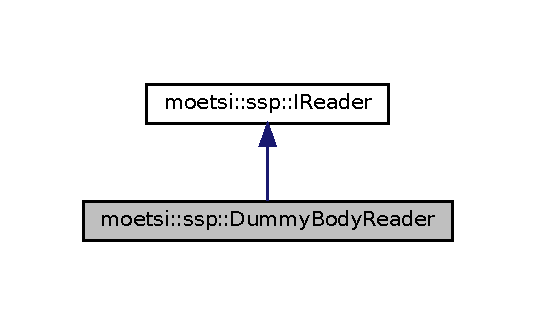
\includegraphics[width=242pt]{classmoetsi_1_1ssp_1_1DummyBodyReader__inherit__graph}
\end{center}
\end{figure}


Collaboration diagram for moetsi\+:\+:ssp\+:\+:Dummy\+Body\+Reader\+:
\nopagebreak
\begin{figure}[H]
\begin{center}
\leavevmode
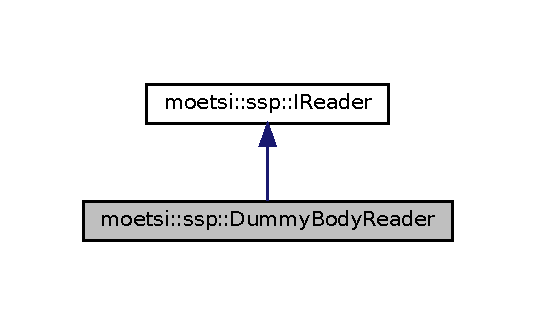
\includegraphics[width=242pt]{classmoetsi_1_1ssp_1_1DummyBodyReader__coll__graph}
\end{center}
\end{figure}
\subsection*{Public Member Functions}
\begin{DoxyCompactItemize}
\item 
\mbox{\Hypertarget{classmoetsi_1_1ssp_1_1DummyBodyReader_ab99ceecb1a406a80dbb80a530a0429af}\label{classmoetsi_1_1ssp_1_1DummyBodyReader_ab99ceecb1a406a80dbb80a530a0429af}} 
virtual std\+::vector$<$ std\+::shared\+\_\+ptr$<$ \hyperlink{structmoetsi_1_1ssp_1_1FrameStruct}{Frame\+Struct} $>$ $>$ \hyperlink{classmoetsi_1_1ssp_1_1DummyBodyReader_ab99ceecb1a406a80dbb80a530a0429af}{Get\+Current\+Frame} ()
\begin{DoxyCompactList}\small\item\em Get current frame data. \end{DoxyCompactList}\item 
virtual std\+::vector$<$ \hyperlink{namespacemoetsi_1_1ssp_a46efdfa2cd5a28ead465dcc8006b5a87}{Frame\+Type} $>$ \hyperlink{classmoetsi_1_1ssp_1_1DummyBodyReader_a2219d7fd14ca1448fb4c6f2541ac3c9b}{Get\+Type} ()
\begin{DoxyCompactList}\small\item\em Get frame types. \end{DoxyCompactList}\item 
virtual bool \hyperlink{classmoetsi_1_1ssp_1_1DummyBodyReader_ab91b3c2ccdba21bae040340c34361595}{Has\+Next\+Frame} ()
\begin{DoxyCompactList}\small\item\em Check if there is a next frame. \end{DoxyCompactList}\item 
\mbox{\Hypertarget{classmoetsi_1_1ssp_1_1DummyBodyReader_a3033d6a22bfcf6ffa86de5477372a5cd}\label{classmoetsi_1_1ssp_1_1DummyBodyReader_a3033d6a22bfcf6ffa86de5477372a5cd}} 
virtual void \hyperlink{classmoetsi_1_1ssp_1_1DummyBodyReader_a3033d6a22bfcf6ffa86de5477372a5cd}{Next\+Frame} ()
\begin{DoxyCompactList}\small\item\em Go to next frame. \end{DoxyCompactList}\item 
\mbox{\Hypertarget{classmoetsi_1_1ssp_1_1DummyBodyReader_ad3334b2dc4730555d90c2a6527a4ca1a}\label{classmoetsi_1_1ssp_1_1DummyBodyReader_ad3334b2dc4730555d90c2a6527a4ca1a}} 
virtual void \hyperlink{classmoetsi_1_1ssp_1_1DummyBodyReader_ad3334b2dc4730555d90c2a6527a4ca1a}{Reset} ()
\begin{DoxyCompactList}\small\item\em Reset this reader. \end{DoxyCompactList}\item 
virtual void \hyperlink{classmoetsi_1_1ssp_1_1DummyBodyReader_a61e495deb7314560d5e17388f6b6938f}{Go\+To\+Frame} (unsigned int frame\+\_\+id)
\begin{DoxyCompactList}\small\item\em Go to a given frame. \end{DoxyCompactList}\item 
virtual unsigned int \hyperlink{classmoetsi_1_1ssp_1_1DummyBodyReader_a91d5b81c241103ffde276d354a34d7db}{Get\+Current\+Frame\+Id} ()
\begin{DoxyCompactList}\small\item\em Get current frame number. \end{DoxyCompactList}\item 
virtual unsigned int \hyperlink{classmoetsi_1_1ssp_1_1DummyBodyReader_a7dab48cb8ec247add0c57d98e6cd5fb4}{Get\+Fps} ()
\begin{DoxyCompactList}\small\item\em Get indicative F\+PS in frame per second. \end{DoxyCompactList}\end{DoxyCompactItemize}


\subsection{Member Function Documentation}
\mbox{\Hypertarget{classmoetsi_1_1ssp_1_1DummyBodyReader_a91d5b81c241103ffde276d354a34d7db}\label{classmoetsi_1_1ssp_1_1DummyBodyReader_a91d5b81c241103ffde276d354a34d7db}} 
\index{moetsi\+::ssp\+::\+Dummy\+Body\+Reader@{moetsi\+::ssp\+::\+Dummy\+Body\+Reader}!Get\+Current\+Frame\+Id@{Get\+Current\+Frame\+Id}}
\index{Get\+Current\+Frame\+Id@{Get\+Current\+Frame\+Id}!moetsi\+::ssp\+::\+Dummy\+Body\+Reader@{moetsi\+::ssp\+::\+Dummy\+Body\+Reader}}
\subsubsection{\texorpdfstring{Get\+Current\+Frame\+Id()}{GetCurrentFrameId()}}
{\footnotesize\ttfamily unsigned int moetsi\+::ssp\+::\+Dummy\+Body\+Reader\+::\+Get\+Current\+Frame\+Id (\begin{DoxyParamCaption}{ }\end{DoxyParamCaption})\hspace{0.3cm}{\ttfamily [virtual]}}



Get current frame number. 

\begin{DoxyReturn}{Returns}
current frame number. 
\end{DoxyReturn}


Implements \hyperlink{classmoetsi_1_1ssp_1_1IReader_ac292d83eb06dee277baaa06e281a562d}{moetsi\+::ssp\+::\+I\+Reader}.

\mbox{\Hypertarget{classmoetsi_1_1ssp_1_1DummyBodyReader_a7dab48cb8ec247add0c57d98e6cd5fb4}\label{classmoetsi_1_1ssp_1_1DummyBodyReader_a7dab48cb8ec247add0c57d98e6cd5fb4}} 
\index{moetsi\+::ssp\+::\+Dummy\+Body\+Reader@{moetsi\+::ssp\+::\+Dummy\+Body\+Reader}!Get\+Fps@{Get\+Fps}}
\index{Get\+Fps@{Get\+Fps}!moetsi\+::ssp\+::\+Dummy\+Body\+Reader@{moetsi\+::ssp\+::\+Dummy\+Body\+Reader}}
\subsubsection{\texorpdfstring{Get\+Fps()}{GetFps()}}
{\footnotesize\ttfamily unsigned int moetsi\+::ssp\+::\+Dummy\+Body\+Reader\+::\+Get\+Fps (\begin{DoxyParamCaption}{ }\end{DoxyParamCaption})\hspace{0.3cm}{\ttfamily [virtual]}}



Get indicative F\+PS in frame per second. 

\begin{DoxyReturn}{Returns}
the F\+PS number 
\end{DoxyReturn}


Implements \hyperlink{classmoetsi_1_1ssp_1_1IReader_a9f6a8650ca290b011b8e5451eeae9f32}{moetsi\+::ssp\+::\+I\+Reader}.

\mbox{\Hypertarget{classmoetsi_1_1ssp_1_1DummyBodyReader_a2219d7fd14ca1448fb4c6f2541ac3c9b}\label{classmoetsi_1_1ssp_1_1DummyBodyReader_a2219d7fd14ca1448fb4c6f2541ac3c9b}} 
\index{moetsi\+::ssp\+::\+Dummy\+Body\+Reader@{moetsi\+::ssp\+::\+Dummy\+Body\+Reader}!Get\+Type@{Get\+Type}}
\index{Get\+Type@{Get\+Type}!moetsi\+::ssp\+::\+Dummy\+Body\+Reader@{moetsi\+::ssp\+::\+Dummy\+Body\+Reader}}
\subsubsection{\texorpdfstring{Get\+Type()}{GetType()}}
{\footnotesize\ttfamily std\+::vector$<$ \hyperlink{namespacemoetsi_1_1ssp_a46efdfa2cd5a28ead465dcc8006b5a87}{Frame\+Type} $>$ moetsi\+::ssp\+::\+Dummy\+Body\+Reader\+::\+Get\+Type (\begin{DoxyParamCaption}{ }\end{DoxyParamCaption})\hspace{0.3cm}{\ttfamily [virtual]}}



Get frame types. 

\begin{DoxyReturn}{Returns}
a vector of Frame\+Type, listing available data types 
\end{DoxyReturn}


Implements \hyperlink{classmoetsi_1_1ssp_1_1IReader_a4116c1931fde7bd66133934ffdca1cce}{moetsi\+::ssp\+::\+I\+Reader}.

\mbox{\Hypertarget{classmoetsi_1_1ssp_1_1DummyBodyReader_a61e495deb7314560d5e17388f6b6938f}\label{classmoetsi_1_1ssp_1_1DummyBodyReader_a61e495deb7314560d5e17388f6b6938f}} 
\index{moetsi\+::ssp\+::\+Dummy\+Body\+Reader@{moetsi\+::ssp\+::\+Dummy\+Body\+Reader}!Go\+To\+Frame@{Go\+To\+Frame}}
\index{Go\+To\+Frame@{Go\+To\+Frame}!moetsi\+::ssp\+::\+Dummy\+Body\+Reader@{moetsi\+::ssp\+::\+Dummy\+Body\+Reader}}
\subsubsection{\texorpdfstring{Go\+To\+Frame()}{GoToFrame()}}
{\footnotesize\ttfamily void moetsi\+::ssp\+::\+Dummy\+Body\+Reader\+::\+Go\+To\+Frame (\begin{DoxyParamCaption}\item[{unsigned int}]{frame\+\_\+id }\end{DoxyParamCaption})\hspace{0.3cm}{\ttfamily [virtual]}}



Go to a given frame. 


\begin{DoxyParams}{Parameters}
{\em frame\+\_\+id} & target frame number \\
\hline
\end{DoxyParams}


Implements \hyperlink{classmoetsi_1_1ssp_1_1IReader_a6f1be3c06538992cca6d550bd9566681}{moetsi\+::ssp\+::\+I\+Reader}.

\mbox{\Hypertarget{classmoetsi_1_1ssp_1_1DummyBodyReader_ab91b3c2ccdba21bae040340c34361595}\label{classmoetsi_1_1ssp_1_1DummyBodyReader_ab91b3c2ccdba21bae040340c34361595}} 
\index{moetsi\+::ssp\+::\+Dummy\+Body\+Reader@{moetsi\+::ssp\+::\+Dummy\+Body\+Reader}!Has\+Next\+Frame@{Has\+Next\+Frame}}
\index{Has\+Next\+Frame@{Has\+Next\+Frame}!moetsi\+::ssp\+::\+Dummy\+Body\+Reader@{moetsi\+::ssp\+::\+Dummy\+Body\+Reader}}
\subsubsection{\texorpdfstring{Has\+Next\+Frame()}{HasNextFrame()}}
{\footnotesize\ttfamily bool moetsi\+::ssp\+::\+Dummy\+Body\+Reader\+::\+Has\+Next\+Frame (\begin{DoxyParamCaption}{ }\end{DoxyParamCaption})\hspace{0.3cm}{\ttfamily [virtual]}}



Check if there is a next frame. 

\begin{DoxyReturn}{Returns}
true if there is a next frame 
\end{DoxyReturn}


Implements \hyperlink{classmoetsi_1_1ssp_1_1IReader_af9186ba41e136dc4ec3242b5dd55fa04}{moetsi\+::ssp\+::\+I\+Reader}.



The documentation for this class was generated from the following files\+:\begin{DoxyCompactItemize}
\item 
\hyperlink{dummy__body__reader_8h}{dummy\+\_\+body\+\_\+reader.\+h}\item 
\hyperlink{dummy__body__reader_8cc}{dummy\+\_\+body\+\_\+reader.\+cc}\end{DoxyCompactItemize}

\hypertarget{structmoetsi_1_1ssp_1_1ExtendedAzureConfig}{}\section{moetsi\+:\+:ssp\+:\+:Extended\+Azure\+Config Struct Reference}
\label{structmoetsi_1_1ssp_1_1ExtendedAzureConfig}\index{moetsi\+::ssp\+::\+Extended\+Azure\+Config@{moetsi\+::ssp\+::\+Extended\+Azure\+Config}}


Azure Kinect configuration.  




{\ttfamily \#include $<$kinect\+\_\+utils.\+h$>$}

\subsection*{Public Attributes}
\begin{DoxyCompactItemize}
\item 
k4a\+\_\+device\+\_\+configuration\+\_\+t \hyperlink{structmoetsi_1_1ssp_1_1ExtendedAzureConfig_a59803eec12939eece3811e3e5d2169e8}{device\+\_\+config}
\item 
bool \hyperlink{structmoetsi_1_1ssp_1_1ExtendedAzureConfig_a602b49142877ef3f88972153cb1478d1}{stream\+\_\+color}
\item 
bool \hyperlink{structmoetsi_1_1ssp_1_1ExtendedAzureConfig_ae189c45e7f654e635d802713814cda3e}{stream\+\_\+depth}
\item 
bool \hyperlink{structmoetsi_1_1ssp_1_1ExtendedAzureConfig_ab4c4fd8a25fe1a5c97aace78bc6d987c}{stream\+\_\+ir}
\item 
int \hyperlink{structmoetsi_1_1ssp_1_1ExtendedAzureConfig_acc60c61ea4d7717f1982f177c56662ea}{absolute\+\_\+exposure\+\_\+value}
\end{DoxyCompactItemize}


\subsection{Detailed Description}
Azure Kinect configuration. 

\subsection{Member Data Documentation}
\mbox{\Hypertarget{structmoetsi_1_1ssp_1_1ExtendedAzureConfig_acc60c61ea4d7717f1982f177c56662ea}\label{structmoetsi_1_1ssp_1_1ExtendedAzureConfig_acc60c61ea4d7717f1982f177c56662ea}} 
\index{moetsi\+::ssp\+::\+Extended\+Azure\+Config@{moetsi\+::ssp\+::\+Extended\+Azure\+Config}!absolute\+\_\+exposure\+\_\+value@{absolute\+\_\+exposure\+\_\+value}}
\index{absolute\+\_\+exposure\+\_\+value@{absolute\+\_\+exposure\+\_\+value}!moetsi\+::ssp\+::\+Extended\+Azure\+Config@{moetsi\+::ssp\+::\+Extended\+Azure\+Config}}
\subsubsection{\texorpdfstring{absolute\+\_\+exposure\+\_\+value}{absolute\_exposure\_value}}
{\footnotesize\ttfamily int moetsi\+::ssp\+::\+Extended\+Azure\+Config\+::absolute\+\_\+exposure\+\_\+value}

Absolute exposure value \mbox{\Hypertarget{structmoetsi_1_1ssp_1_1ExtendedAzureConfig_a59803eec12939eece3811e3e5d2169e8}\label{structmoetsi_1_1ssp_1_1ExtendedAzureConfig_a59803eec12939eece3811e3e5d2169e8}} 
\index{moetsi\+::ssp\+::\+Extended\+Azure\+Config@{moetsi\+::ssp\+::\+Extended\+Azure\+Config}!device\+\_\+config@{device\+\_\+config}}
\index{device\+\_\+config@{device\+\_\+config}!moetsi\+::ssp\+::\+Extended\+Azure\+Config@{moetsi\+::ssp\+::\+Extended\+Azure\+Config}}
\subsubsection{\texorpdfstring{device\+\_\+config}{device\_config}}
{\footnotesize\ttfamily k4a\+\_\+device\+\_\+configuration\+\_\+t moetsi\+::ssp\+::\+Extended\+Azure\+Config\+::device\+\_\+config}

Device configuration \mbox{\Hypertarget{structmoetsi_1_1ssp_1_1ExtendedAzureConfig_a602b49142877ef3f88972153cb1478d1}\label{structmoetsi_1_1ssp_1_1ExtendedAzureConfig_a602b49142877ef3f88972153cb1478d1}} 
\index{moetsi\+::ssp\+::\+Extended\+Azure\+Config@{moetsi\+::ssp\+::\+Extended\+Azure\+Config}!stream\+\_\+color@{stream\+\_\+color}}
\index{stream\+\_\+color@{stream\+\_\+color}!moetsi\+::ssp\+::\+Extended\+Azure\+Config@{moetsi\+::ssp\+::\+Extended\+Azure\+Config}}
\subsubsection{\texorpdfstring{stream\+\_\+color}{stream\_color}}
{\footnotesize\ttfamily bool moetsi\+::ssp\+::\+Extended\+Azure\+Config\+::stream\+\_\+color}

If true, stream color frames \mbox{\Hypertarget{structmoetsi_1_1ssp_1_1ExtendedAzureConfig_ae189c45e7f654e635d802713814cda3e}\label{structmoetsi_1_1ssp_1_1ExtendedAzureConfig_ae189c45e7f654e635d802713814cda3e}} 
\index{moetsi\+::ssp\+::\+Extended\+Azure\+Config@{moetsi\+::ssp\+::\+Extended\+Azure\+Config}!stream\+\_\+depth@{stream\+\_\+depth}}
\index{stream\+\_\+depth@{stream\+\_\+depth}!moetsi\+::ssp\+::\+Extended\+Azure\+Config@{moetsi\+::ssp\+::\+Extended\+Azure\+Config}}
\subsubsection{\texorpdfstring{stream\+\_\+depth}{stream\_depth}}
{\footnotesize\ttfamily bool moetsi\+::ssp\+::\+Extended\+Azure\+Config\+::stream\+\_\+depth}

If true, stream depth frames \mbox{\Hypertarget{structmoetsi_1_1ssp_1_1ExtendedAzureConfig_ab4c4fd8a25fe1a5c97aace78bc6d987c}\label{structmoetsi_1_1ssp_1_1ExtendedAzureConfig_ab4c4fd8a25fe1a5c97aace78bc6d987c}} 
\index{moetsi\+::ssp\+::\+Extended\+Azure\+Config@{moetsi\+::ssp\+::\+Extended\+Azure\+Config}!stream\+\_\+ir@{stream\+\_\+ir}}
\index{stream\+\_\+ir@{stream\+\_\+ir}!moetsi\+::ssp\+::\+Extended\+Azure\+Config@{moetsi\+::ssp\+::\+Extended\+Azure\+Config}}
\subsubsection{\texorpdfstring{stream\+\_\+ir}{stream\_ir}}
{\footnotesize\ttfamily bool moetsi\+::ssp\+::\+Extended\+Azure\+Config\+::stream\+\_\+ir}

If true, stream infrared frames 

The documentation for this struct was generated from the following file\+:\begin{DoxyCompactItemize}
\item 
\hyperlink{kinect__utils_8h}{kinect\+\_\+utils.\+h}\end{DoxyCompactItemize}

\hypertarget{structmoetsi_1_1ssp_1_1FrameStruct}{}\section{moetsi\+:\+:ssp\+:\+:Frame\+Struct Struct Reference}
\label{structmoetsi_1_1ssp_1_1FrameStruct}\index{moetsi\+::ssp\+::\+Frame\+Struct@{moetsi\+::ssp\+::\+Frame\+Struct}}


Frame struct\+: S\+SP frame.  




{\ttfamily \#include $<$frame\+\_\+struct.\+h$>$}



Collaboration diagram for moetsi\+:\+:ssp\+:\+:Frame\+Struct\+:
\nopagebreak
\begin{figure}[H]
\begin{center}
\leavevmode
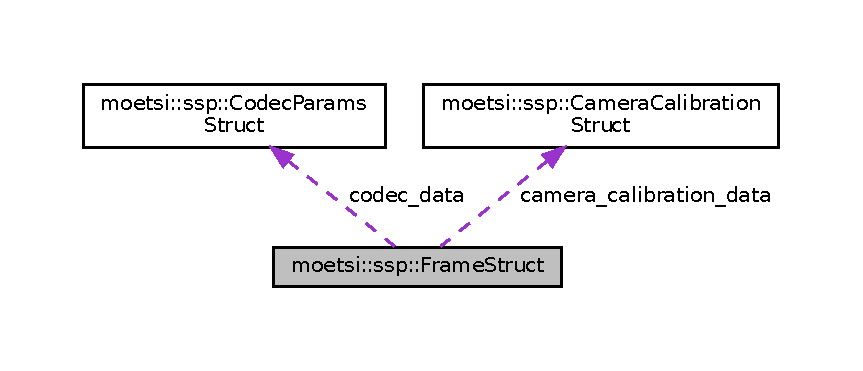
\includegraphics[width=350pt]{structmoetsi_1_1ssp_1_1FrameStruct__coll__graph}
\end{center}
\end{figure}
\subsection*{Public Member Functions}
\begin{DoxyCompactItemize}
\item 
\mbox{\Hypertarget{structmoetsi_1_1ssp_1_1FrameStruct_af53f4e76978e2a4575b7cd661d30e01f}\label{structmoetsi_1_1ssp_1_1FrameStruct_af53f4e76978e2a4575b7cd661d30e01f}} 
{\footnotesize template$<$class Archive $>$ }\\void {\bfseries serialize} (Archive \&ar)
\item 
\mbox{\Hypertarget{structmoetsi_1_1ssp_1_1FrameStruct_af53f4e76978e2a4575b7cd661d30e01f}\label{structmoetsi_1_1ssp_1_1FrameStruct_af53f4e76978e2a4575b7cd661d30e01f}} 
{\footnotesize template$<$class Archive $>$ }\\void {\bfseries serialize} (Archive \&ar)
\end{DoxyCompactItemize}
\subsection*{Public Attributes}
\begin{DoxyCompactItemize}
\item 
\hyperlink{namespacemoetsi_1_1ssp_a8948545ffe48a5b3507fd10a1e56d546}{S\+S\+P\+Message\+Type} \hyperlink{structmoetsi_1_1ssp_1_1FrameStruct_a6c6ff38e4cbbf4e3af7cdcb6192e8ba8}{message\+\_\+type}
\item 
\hyperlink{namespacemoetsi_1_1ssp_a46efdfa2cd5a28ead465dcc8006b5a87}{Frame\+Type} \hyperlink{structmoetsi_1_1ssp_1_1FrameStruct_ac7fe0bfa84d7492827728c49544fc0a2}{frame\+\_\+type}
\item 
\hyperlink{namespacemoetsi_1_1ssp_aa9b059f0bc7a91855545ee887f2d56c4}{Frame\+Data\+Type} \hyperlink{structmoetsi_1_1ssp_1_1FrameStruct_a281ef582bcbb8b6b3d0f0eb3efd615c6}{frame\+\_\+data\+\_\+type}
\item 
std\+::string \hyperlink{structmoetsi_1_1ssp_1_1FrameStruct_a14a7976abfb26a9ca42e17555f8b1a8c}{stream\+\_\+id}
\item 
std\+::vector$<$ unsigned char $>$ \hyperlink{structmoetsi_1_1ssp_1_1FrameStruct_a7556ce8749c65cd5b22ea9c7a4c17619}{frame}
\item 
\hyperlink{structmoetsi_1_1ssp_1_1CodecParamsStruct}{Codec\+Params\+Struct} \hyperlink{structmoetsi_1_1ssp_1_1FrameStruct_a84ed01cb3227bcece29c43ba8ec322ee}{codec\+\_\+data}
\item 
\hyperlink{structmoetsi_1_1ssp_1_1CameraCalibrationStruct}{Camera\+Calibration\+Struct} \hyperlink{structmoetsi_1_1ssp_1_1FrameStruct_acbdc93c52c66264ed3f4c06a088c955d}{camera\+\_\+calibration\+\_\+data}
\item 
std\+::string \hyperlink{structmoetsi_1_1ssp_1_1FrameStruct_a7e717ab7290ddbb430c3c5a8858ddac6}{scene\+\_\+desc}
\item 
unsigned int \hyperlink{structmoetsi_1_1ssp_1_1FrameStruct_ae585f1be534924a69c8617b2f5f83568}{sensor\+\_\+id}
\item 
unsigned int \hyperlink{structmoetsi_1_1ssp_1_1FrameStruct_af3b1ea702009be5df748af30a159a38a}{device\+\_\+id}
\item 
unsigned int \hyperlink{structmoetsi_1_1ssp_1_1FrameStruct_aebc84f95b5024225412d92a56ddf24ad}{frame\+\_\+id}
\item 
std\+::vector$<$ uint64\+\_\+t $>$ \hyperlink{structmoetsi_1_1ssp_1_1FrameStruct_aa445729218d4963e527377d760ac8015}{timestamps}
\end{DoxyCompactItemize}


\subsection{Detailed Description}
Frame struct\+: S\+SP frame. 

\subsection{Member Data Documentation}
\mbox{\Hypertarget{structmoetsi_1_1ssp_1_1FrameStruct_acbdc93c52c66264ed3f4c06a088c955d}\label{structmoetsi_1_1ssp_1_1FrameStruct_acbdc93c52c66264ed3f4c06a088c955d}} 
\index{moetsi\+::ssp\+::\+Frame\+Struct@{moetsi\+::ssp\+::\+Frame\+Struct}!camera\+\_\+calibration\+\_\+data@{camera\+\_\+calibration\+\_\+data}}
\index{camera\+\_\+calibration\+\_\+data@{camera\+\_\+calibration\+\_\+data}!moetsi\+::ssp\+::\+Frame\+Struct@{moetsi\+::ssp\+::\+Frame\+Struct}}
\subsubsection{\texorpdfstring{camera\+\_\+calibration\+\_\+data}{camera\_calibration\_data}}
{\footnotesize\ttfamily \hyperlink{structmoetsi_1_1ssp_1_1CameraCalibrationStruct}{Camera\+Calibration\+Struct} moetsi\+::ssp\+::\+Frame\+Struct\+::camera\+\_\+calibration\+\_\+data}

Codec info for video frames, null for image frames \mbox{\Hypertarget{structmoetsi_1_1ssp_1_1FrameStruct_a84ed01cb3227bcece29c43ba8ec322ee}\label{structmoetsi_1_1ssp_1_1FrameStruct_a84ed01cb3227bcece29c43ba8ec322ee}} 
\index{moetsi\+::ssp\+::\+Frame\+Struct@{moetsi\+::ssp\+::\+Frame\+Struct}!codec\+\_\+data@{codec\+\_\+data}}
\index{codec\+\_\+data@{codec\+\_\+data}!moetsi\+::ssp\+::\+Frame\+Struct@{moetsi\+::ssp\+::\+Frame\+Struct}}
\subsubsection{\texorpdfstring{codec\+\_\+data}{codec\_data}}
{\footnotesize\ttfamily \hyperlink{structmoetsi_1_1ssp_1_1CodecParamsStruct}{Codec\+Params\+Struct} moetsi\+::ssp\+::\+Frame\+Struct\+::codec\+\_\+data}

Codec info for video frames, null for image frames Video decoder needs to know about the last receive frame Requires to know the codec as well as additional parameters \mbox{\Hypertarget{structmoetsi_1_1ssp_1_1FrameStruct_af3b1ea702009be5df748af30a159a38a}\label{structmoetsi_1_1ssp_1_1FrameStruct_af3b1ea702009be5df748af30a159a38a}} 
\index{moetsi\+::ssp\+::\+Frame\+Struct@{moetsi\+::ssp\+::\+Frame\+Struct}!device\+\_\+id@{device\+\_\+id}}
\index{device\+\_\+id@{device\+\_\+id}!moetsi\+::ssp\+::\+Frame\+Struct@{moetsi\+::ssp\+::\+Frame\+Struct}}
\subsubsection{\texorpdfstring{device\+\_\+id}{device\_id}}
{\footnotesize\ttfamily unsigned int moetsi\+::ssp\+::\+Frame\+Struct\+::device\+\_\+id}

Integer device id\+: distingish between devices in the same scene Can be set by user. \mbox{\Hypertarget{structmoetsi_1_1ssp_1_1FrameStruct_a7556ce8749c65cd5b22ea9c7a4c17619}\label{structmoetsi_1_1ssp_1_1FrameStruct_a7556ce8749c65cd5b22ea9c7a4c17619}} 
\index{moetsi\+::ssp\+::\+Frame\+Struct@{moetsi\+::ssp\+::\+Frame\+Struct}!frame@{frame}}
\index{frame@{frame}!moetsi\+::ssp\+::\+Frame\+Struct@{moetsi\+::ssp\+::\+Frame\+Struct}}
\subsubsection{\texorpdfstring{frame}{frame}}
{\footnotesize\ttfamily std\+::vector$<$ unsigned char $>$ moetsi\+::ssp\+::\+Frame\+Struct\+::frame}

Frame binary data We use a vector to know the size, basically a vector of bytes to store binary data \mbox{\Hypertarget{structmoetsi_1_1ssp_1_1FrameStruct_a281ef582bcbb8b6b3d0f0eb3efd615c6}\label{structmoetsi_1_1ssp_1_1FrameStruct_a281ef582bcbb8b6b3d0f0eb3efd615c6}} 
\index{moetsi\+::ssp\+::\+Frame\+Struct@{moetsi\+::ssp\+::\+Frame\+Struct}!frame\+\_\+data\+\_\+type@{frame\+\_\+data\+\_\+type}}
\index{frame\+\_\+data\+\_\+type@{frame\+\_\+data\+\_\+type}!moetsi\+::ssp\+::\+Frame\+Struct@{moetsi\+::ssp\+::\+Frame\+Struct}}
\subsubsection{\texorpdfstring{frame\+\_\+data\+\_\+type}{frame\_data\_type}}
{\footnotesize\ttfamily \hyperlink{namespacemoetsi_1_1ssp_aa9b059f0bc7a91855545ee887f2d56c4}{Frame\+Data\+Type} moetsi\+::ssp\+::\+Frame\+Struct\+::frame\+\_\+data\+\_\+type}

Frame data type \mbox{\Hypertarget{structmoetsi_1_1ssp_1_1FrameStruct_aebc84f95b5024225412d92a56ddf24ad}\label{structmoetsi_1_1ssp_1_1FrameStruct_aebc84f95b5024225412d92a56ddf24ad}} 
\index{moetsi\+::ssp\+::\+Frame\+Struct@{moetsi\+::ssp\+::\+Frame\+Struct}!frame\+\_\+id@{frame\+\_\+id}}
\index{frame\+\_\+id@{frame\+\_\+id}!moetsi\+::ssp\+::\+Frame\+Struct@{moetsi\+::ssp\+::\+Frame\+Struct}}
\subsubsection{\texorpdfstring{frame\+\_\+id}{frame\_id}}
{\footnotesize\ttfamily unsigned int moetsi\+::ssp\+::\+Frame\+Struct\+::frame\+\_\+id}

Current frame number (increases over time) Increases by 1 for each frame automatically when S\+SP server starts \mbox{\Hypertarget{structmoetsi_1_1ssp_1_1FrameStruct_ac7fe0bfa84d7492827728c49544fc0a2}\label{structmoetsi_1_1ssp_1_1FrameStruct_ac7fe0bfa84d7492827728c49544fc0a2}} 
\index{moetsi\+::ssp\+::\+Frame\+Struct@{moetsi\+::ssp\+::\+Frame\+Struct}!frame\+\_\+type@{frame\+\_\+type}}
\index{frame\+\_\+type@{frame\+\_\+type}!moetsi\+::ssp\+::\+Frame\+Struct@{moetsi\+::ssp\+::\+Frame\+Struct}}
\subsubsection{\texorpdfstring{frame\+\_\+type}{frame\_type}}
{\footnotesize\ttfamily \hyperlink{namespacemoetsi_1_1ssp_a46efdfa2cd5a28ead465dcc8006b5a87}{Frame\+Type} moetsi\+::ssp\+::\+Frame\+Struct\+::frame\+\_\+type}

Frame type \mbox{\Hypertarget{structmoetsi_1_1ssp_1_1FrameStruct_a6c6ff38e4cbbf4e3af7cdcb6192e8ba8}\label{structmoetsi_1_1ssp_1_1FrameStruct_a6c6ff38e4cbbf4e3af7cdcb6192e8ba8}} 
\index{moetsi\+::ssp\+::\+Frame\+Struct@{moetsi\+::ssp\+::\+Frame\+Struct}!message\+\_\+type@{message\+\_\+type}}
\index{message\+\_\+type@{message\+\_\+type}!moetsi\+::ssp\+::\+Frame\+Struct@{moetsi\+::ssp\+::\+Frame\+Struct}}
\subsubsection{\texorpdfstring{message\+\_\+type}{message\_type}}
{\footnotesize\ttfamily \hyperlink{namespacemoetsi_1_1ssp_a8948545ffe48a5b3507fd10a1e56d546}{S\+S\+P\+Message\+Type} moetsi\+::ssp\+::\+Frame\+Struct\+::message\+\_\+type}

S\+SP message type \mbox{\Hypertarget{structmoetsi_1_1ssp_1_1FrameStruct_a7e717ab7290ddbb430c3c5a8858ddac6}\label{structmoetsi_1_1ssp_1_1FrameStruct_a7e717ab7290ddbb430c3c5a8858ddac6}} 
\index{moetsi\+::ssp\+::\+Frame\+Struct@{moetsi\+::ssp\+::\+Frame\+Struct}!scene\+\_\+desc@{scene\+\_\+desc}}
\index{scene\+\_\+desc@{scene\+\_\+desc}!moetsi\+::ssp\+::\+Frame\+Struct@{moetsi\+::ssp\+::\+Frame\+Struct}}
\subsubsection{\texorpdfstring{scene\+\_\+desc}{scene\_desc}}
{\footnotesize\ttfamily std\+::string moetsi\+::ssp\+::\+Frame\+Struct\+::scene\+\_\+desc}

Optional\+: scene description \mbox{\Hypertarget{structmoetsi_1_1ssp_1_1FrameStruct_ae585f1be534924a69c8617b2f5f83568}\label{structmoetsi_1_1ssp_1_1FrameStruct_ae585f1be534924a69c8617b2f5f83568}} 
\index{moetsi\+::ssp\+::\+Frame\+Struct@{moetsi\+::ssp\+::\+Frame\+Struct}!sensor\+\_\+id@{sensor\+\_\+id}}
\index{sensor\+\_\+id@{sensor\+\_\+id}!moetsi\+::ssp\+::\+Frame\+Struct@{moetsi\+::ssp\+::\+Frame\+Struct}}
\subsubsection{\texorpdfstring{sensor\+\_\+id}{sensor\_id}}
{\footnotesize\ttfamily unsigned int moetsi\+::ssp\+::\+Frame\+Struct\+::sensor\+\_\+id}

Sensor id \mbox{\Hypertarget{structmoetsi_1_1ssp_1_1FrameStruct_a14a7976abfb26a9ca42e17555f8b1a8c}\label{structmoetsi_1_1ssp_1_1FrameStruct_a14a7976abfb26a9ca42e17555f8b1a8c}} 
\index{moetsi\+::ssp\+::\+Frame\+Struct@{moetsi\+::ssp\+::\+Frame\+Struct}!stream\+\_\+id@{stream\+\_\+id}}
\index{stream\+\_\+id@{stream\+\_\+id}!moetsi\+::ssp\+::\+Frame\+Struct@{moetsi\+::ssp\+::\+Frame\+Struct}}
\subsubsection{\texorpdfstring{stream\+\_\+id}{stream\_id}}
{\footnotesize\ttfamily std\+::string moetsi\+::ssp\+::\+Frame\+Struct\+::stream\+\_\+id}

Random 16 char string that uniquely ids the frame stream. Some decoders (like video) are stateful and so must keep track of streams. This is automatically generated. \mbox{\Hypertarget{structmoetsi_1_1ssp_1_1FrameStruct_aa445729218d4963e527377d760ac8015}\label{structmoetsi_1_1ssp_1_1FrameStruct_aa445729218d4963e527377d760ac8015}} 
\index{moetsi\+::ssp\+::\+Frame\+Struct@{moetsi\+::ssp\+::\+Frame\+Struct}!timestamps@{timestamps}}
\index{timestamps@{timestamps}!moetsi\+::ssp\+::\+Frame\+Struct@{moetsi\+::ssp\+::\+Frame\+Struct}}
\subsubsection{\texorpdfstring{timestamps}{timestamps}}
{\footnotesize\ttfamily std\+::vector$<$ uint64\+\_\+t $>$ moetsi\+::ssp\+::\+Frame\+Struct\+::timestamps}

Use for logging and timing to understand processing speeds. Times are in ns 

The documentation for this struct was generated from the following file\+:\begin{DoxyCompactItemize}
\item 
include/structs/frame\+\_\+struct.\+h\end{DoxyCompactItemize}

\hypertarget{classmoetsi_1_1ssp_1_1IDecoder}{}\doxysection{moetsi\+::ssp\+::I\+Decoder Class Reference}
\label{classmoetsi_1_1ssp_1_1IDecoder}\index{moetsi::ssp::IDecoder@{moetsi::ssp::IDecoder}}


\mbox{\hyperlink{classmoetsi_1_1ssp_1_1IDecoder}{I\+Decoder}} abstract decoder interface.  




{\ttfamily \#include $<$idecoder.\+h$>$}



Inheritance diagram for moetsi\+::ssp\+::I\+Decoder\+:
% FIG 0
\doxysubsection*{Public Member Functions}
\begin{DoxyCompactItemize}
\item 
\mbox{\Hypertarget{classmoetsi_1_1ssp_1_1IDecoder_a26dc991c2434792f50ec5ae9b61a1653}\label{classmoetsi_1_1ssp_1_1IDecoder_a26dc991c2434792f50ec5ae9b61a1653}} 
virtual \mbox{\hyperlink{classmoetsi_1_1ssp_1_1IDecoder_a26dc991c2434792f50ec5ae9b61a1653}{$\sim$\+I\+Decoder}} ()
\begin{DoxyCompactList}\small\item\em Virtual destructor. \end{DoxyCompactList}\item 
virtual cv\+::\+Mat \mbox{\hyperlink{classmoetsi_1_1ssp_1_1IDecoder_a1c06604dc4107d3668a4e791c13cc063}{Decode}} (\mbox{\hyperlink{structmoetsi_1_1ssp_1_1FrameStruct}{Frame\+Struct}} \&data)=0
\begin{DoxyCompactList}\small\item\em Extract an opencv image from a \mbox{\hyperlink{structmoetsi_1_1ssp_1_1FrameStruct}{Frame\+Struct}}. \end{DoxyCompactList}\item 
\mbox{\Hypertarget{classmoetsi_1_1ssp_1_1IDecoder_a26dc991c2434792f50ec5ae9b61a1653}\label{classmoetsi_1_1ssp_1_1IDecoder_a26dc991c2434792f50ec5ae9b61a1653}} 
virtual \mbox{\hyperlink{classmoetsi_1_1ssp_1_1IDecoder_a26dc991c2434792f50ec5ae9b61a1653}{$\sim$\+I\+Decoder}} ()
\begin{DoxyCompactList}\small\item\em Virtual destructor. \end{DoxyCompactList}\item 
virtual cv\+::\+Mat \mbox{\hyperlink{classmoetsi_1_1ssp_1_1IDecoder_a1c06604dc4107d3668a4e791c13cc063}{Decode}} (\mbox{\hyperlink{structmoetsi_1_1ssp_1_1FrameStruct}{Frame\+Struct}} \&data)=0
\begin{DoxyCompactList}\small\item\em Extract an opencv image from a \mbox{\hyperlink{structmoetsi_1_1ssp_1_1FrameStruct}{Frame\+Struct}}. \end{DoxyCompactList}\end{DoxyCompactItemize}


\doxysubsection{Detailed Description}
\mbox{\hyperlink{classmoetsi_1_1ssp_1_1IDecoder}{I\+Decoder}} abstract decoder interface. 

\doxysubsection{Member Function Documentation}
\mbox{\Hypertarget{classmoetsi_1_1ssp_1_1IDecoder_a1c06604dc4107d3668a4e791c13cc063}\label{classmoetsi_1_1ssp_1_1IDecoder_a1c06604dc4107d3668a4e791c13cc063}} 
\index{moetsi::ssp::IDecoder@{moetsi::ssp::IDecoder}!Decode@{Decode}}
\index{Decode@{Decode}!moetsi::ssp::IDecoder@{moetsi::ssp::IDecoder}}
\doxysubsubsection{\texorpdfstring{Decode()}{Decode()}\hspace{0.1cm}{\footnotesize\ttfamily [1/2]}}
{\footnotesize\ttfamily virtual cv\+::\+Mat moetsi\+::ssp\+::\+I\+Decoder\+::\+Decode (\begin{DoxyParamCaption}\item[{\mbox{\hyperlink{structmoetsi_1_1ssp_1_1FrameStruct}{Frame\+Struct}} \&}]{data }\end{DoxyParamCaption})\hspace{0.3cm}{\ttfamily [pure virtual]}}



Extract an opencv image from a \mbox{\hyperlink{structmoetsi_1_1ssp_1_1FrameStruct}{Frame\+Struct}}. 


\begin{DoxyParams}{Parameters}
{\em data} & \mbox{\hyperlink{structmoetsi_1_1ssp_1_1FrameStruct}{Frame\+Struct}} \\
\hline
\end{DoxyParams}
\begin{DoxyReturn}{Returns}
Open\+CV matrix/image 
\end{DoxyReturn}


Implemented in \mbox{\hyperlink{classmoetsi_1_1ssp_1_1LibAvDecoder_a4206a4581de1b93d6c6a0835e8cf4ac8}{moetsi\+::ssp\+::\+Lib\+Av\+Decoder}}, \mbox{\hyperlink{classmoetsi_1_1ssp_1_1NvDecoder_a78eb894b6825ac5ec57f5a4f4ecd7e31}{moetsi\+::ssp\+::\+Nv\+Decoder}}, and \mbox{\hyperlink{classmoetsi_1_1ssp_1_1ZDepthDecoder_a43226095658d616f7e38df1d43c2f88a}{moetsi\+::ssp\+::\+Z\+Depth\+Decoder}}.

\mbox{\Hypertarget{classmoetsi_1_1ssp_1_1IDecoder_a1c06604dc4107d3668a4e791c13cc063}\label{classmoetsi_1_1ssp_1_1IDecoder_a1c06604dc4107d3668a4e791c13cc063}} 
\index{moetsi::ssp::IDecoder@{moetsi::ssp::IDecoder}!Decode@{Decode}}
\index{Decode@{Decode}!moetsi::ssp::IDecoder@{moetsi::ssp::IDecoder}}
\doxysubsubsection{\texorpdfstring{Decode()}{Decode()}\hspace{0.1cm}{\footnotesize\ttfamily [2/2]}}
{\footnotesize\ttfamily virtual cv\+::\+Mat moetsi\+::ssp\+::\+I\+Decoder\+::\+Decode (\begin{DoxyParamCaption}\item[{\mbox{\hyperlink{structmoetsi_1_1ssp_1_1FrameStruct}{Frame\+Struct}} \&}]{data }\end{DoxyParamCaption})\hspace{0.3cm}{\ttfamily [pure virtual]}}



Extract an opencv image from a \mbox{\hyperlink{structmoetsi_1_1ssp_1_1FrameStruct}{Frame\+Struct}}. 


\begin{DoxyParams}{Parameters}
{\em data} & \mbox{\hyperlink{structmoetsi_1_1ssp_1_1FrameStruct}{Frame\+Struct}} \\
\hline
\end{DoxyParams}
\begin{DoxyReturn}{Returns}
Open\+CV matrix/image 
\end{DoxyReturn}


Implemented in \mbox{\hyperlink{classmoetsi_1_1ssp_1_1LibAvDecoder_a4206a4581de1b93d6c6a0835e8cf4ac8}{moetsi\+::ssp\+::\+Lib\+Av\+Decoder}}, \mbox{\hyperlink{classmoetsi_1_1ssp_1_1NvDecoder_a78eb894b6825ac5ec57f5a4f4ecd7e31}{moetsi\+::ssp\+::\+Nv\+Decoder}}, and \mbox{\hyperlink{classmoetsi_1_1ssp_1_1ZDepthDecoder_a43226095658d616f7e38df1d43c2f88a}{moetsi\+::ssp\+::\+Z\+Depth\+Decoder}}.



The documentation for this class was generated from the following file\+:\begin{DoxyCompactItemize}
\item 
\mbox{\hyperlink{decoders_2idecoder_8h}{decoders/idecoder.\+h}}\end{DoxyCompactItemize}

\hypertarget{classmoetsi_1_1ssp_1_1IEncoder}{}\doxysection{moetsi\+::ssp\+::I\+Encoder Class Reference}
\label{classmoetsi_1_1ssp_1_1IEncoder}\index{moetsi::ssp::IEncoder@{moetsi::ssp::IEncoder}}


\mbox{\hyperlink{classmoetsi_1_1ssp_1_1IEncoder}{I\+Encoder}} abstract encoder class.  




{\ttfamily \#include $<$iencoder.\+h$>$}



Inheritance diagram for moetsi\+::ssp\+::I\+Encoder\+:
% FIG 0
\doxysubsection*{Public Member Functions}
\begin{DoxyCompactItemize}
\item 
\mbox{\Hypertarget{classmoetsi_1_1ssp_1_1IEncoder_a6c19808ebe6a05dbce630c45188b9346}\label{classmoetsi_1_1ssp_1_1IEncoder_a6c19808ebe6a05dbce630c45188b9346}} 
virtual \mbox{\hyperlink{classmoetsi_1_1ssp_1_1IEncoder_a6c19808ebe6a05dbce630c45188b9346}{$\sim$\+I\+Encoder}} ()
\begin{DoxyCompactList}\small\item\em Virtual destructor. \end{DoxyCompactList}\item 
virtual void \mbox{\hyperlink{classmoetsi_1_1ssp_1_1IEncoder_a8c223ec82fdd30ee8ee75157306054ec}{Add\+Frame\+Struct}} (std\+::shared\+\_\+ptr$<$ \mbox{\hyperlink{structmoetsi_1_1ssp_1_1FrameStruct}{Frame\+Struct}} $>$ \&frame\+\_\+struct)=0
\begin{DoxyCompactList}\small\item\em Add a frame struct. \end{DoxyCompactList}\item 
\mbox{\Hypertarget{classmoetsi_1_1ssp_1_1IEncoder_afac3ddcf2f49be16020c83cb9e0fb274}\label{classmoetsi_1_1ssp_1_1IEncoder_afac3ddcf2f49be16020c83cb9e0fb274}} 
virtual void \mbox{\hyperlink{classmoetsi_1_1ssp_1_1IEncoder_afac3ddcf2f49be16020c83cb9e0fb274}{Next\+Packet}} ()=0
\begin{DoxyCompactList}\small\item\em Go to next packet. \end{DoxyCompactList}\item 
virtual bool \mbox{\hyperlink{classmoetsi_1_1ssp_1_1IEncoder_a2af8e23d841ef61f6ee4037e56a3694d}{Has\+Next\+Packet}} ()=0
\begin{DoxyCompactList}\small\item\em Check if there is a next packet. \end{DoxyCompactList}\item 
virtual std\+::shared\+\_\+ptr$<$ \mbox{\hyperlink{structmoetsi_1_1ssp_1_1FrameStruct}{Frame\+Struct}} $>$ \mbox{\hyperlink{classmoetsi_1_1ssp_1_1IEncoder_a178d117518e7c7007414ea9c82bd3ed6}{Current\+Frame\+Encoded}} ()=0
\begin{DoxyCompactList}\small\item\em Get current encoded frame. \end{DoxyCompactList}\item 
virtual std\+::shared\+\_\+ptr$<$ \mbox{\hyperlink{structmoetsi_1_1ssp_1_1FrameStruct}{Frame\+Struct}} $>$ \mbox{\hyperlink{classmoetsi_1_1ssp_1_1IEncoder_ab60bdaae0a85289dfa31a12bab533dc0}{Current\+Frame\+Original}} ()=0
\begin{DoxyCompactList}\small\item\em Get current frame in its original format. \end{DoxyCompactList}\item 
virtual std\+::shared\+\_\+ptr$<$ \mbox{\hyperlink{structmoetsi_1_1ssp_1_1CodecParamsStruct}{Codec\+Params\+Struct}} $>$ \mbox{\hyperlink{classmoetsi_1_1ssp_1_1IEncoder_ad5179efaa4c74207766dd64f46f4059a}{Get\+Codec\+Params\+Struct}} ()=0
\begin{DoxyCompactList}\small\item\em Get codec parameters. \end{DoxyCompactList}\item 
virtual unsigned int \mbox{\hyperlink{classmoetsi_1_1ssp_1_1IEncoder_ae6a865aa52230d81aed1cb5232402f6c}{Get\+Fps}} ()=0
\begin{DoxyCompactList}\small\item\em Get F\+PS. \end{DoxyCompactList}\item 
\mbox{\Hypertarget{classmoetsi_1_1ssp_1_1IEncoder_a6c19808ebe6a05dbce630c45188b9346}\label{classmoetsi_1_1ssp_1_1IEncoder_a6c19808ebe6a05dbce630c45188b9346}} 
virtual \mbox{\hyperlink{classmoetsi_1_1ssp_1_1IEncoder_a6c19808ebe6a05dbce630c45188b9346}{$\sim$\+I\+Encoder}} ()
\begin{DoxyCompactList}\small\item\em Virtual destructor. \end{DoxyCompactList}\item 
virtual void \mbox{\hyperlink{classmoetsi_1_1ssp_1_1IEncoder_a8c223ec82fdd30ee8ee75157306054ec}{Add\+Frame\+Struct}} (std\+::shared\+\_\+ptr$<$ \mbox{\hyperlink{structmoetsi_1_1ssp_1_1FrameStruct}{Frame\+Struct}} $>$ \&frame\+\_\+struct)=0
\begin{DoxyCompactList}\small\item\em Add a frame struct. \end{DoxyCompactList}\item 
\mbox{\Hypertarget{classmoetsi_1_1ssp_1_1IEncoder_afac3ddcf2f49be16020c83cb9e0fb274}\label{classmoetsi_1_1ssp_1_1IEncoder_afac3ddcf2f49be16020c83cb9e0fb274}} 
virtual void \mbox{\hyperlink{classmoetsi_1_1ssp_1_1IEncoder_afac3ddcf2f49be16020c83cb9e0fb274}{Next\+Packet}} ()=0
\begin{DoxyCompactList}\small\item\em Go to next packet. \end{DoxyCompactList}\item 
virtual bool \mbox{\hyperlink{classmoetsi_1_1ssp_1_1IEncoder_a2af8e23d841ef61f6ee4037e56a3694d}{Has\+Next\+Packet}} ()=0
\begin{DoxyCompactList}\small\item\em Check if there is a next packet. \end{DoxyCompactList}\item 
virtual std\+::shared\+\_\+ptr$<$ \mbox{\hyperlink{structmoetsi_1_1ssp_1_1FrameStruct}{Frame\+Struct}} $>$ \mbox{\hyperlink{classmoetsi_1_1ssp_1_1IEncoder_a178d117518e7c7007414ea9c82bd3ed6}{Current\+Frame\+Encoded}} ()=0
\begin{DoxyCompactList}\small\item\em Get current encoded frame. \end{DoxyCompactList}\item 
virtual std\+::shared\+\_\+ptr$<$ \mbox{\hyperlink{structmoetsi_1_1ssp_1_1FrameStruct}{Frame\+Struct}} $>$ \mbox{\hyperlink{classmoetsi_1_1ssp_1_1IEncoder_ab60bdaae0a85289dfa31a12bab533dc0}{Current\+Frame\+Original}} ()=0
\begin{DoxyCompactList}\small\item\em Get current frame in its original format. \end{DoxyCompactList}\item 
virtual std\+::shared\+\_\+ptr$<$ \mbox{\hyperlink{structmoetsi_1_1ssp_1_1CodecParamsStruct}{Codec\+Params\+Struct}} $>$ \mbox{\hyperlink{classmoetsi_1_1ssp_1_1IEncoder_ad5179efaa4c74207766dd64f46f4059a}{Get\+Codec\+Params\+Struct}} ()=0
\begin{DoxyCompactList}\small\item\em Get codec parameters. \end{DoxyCompactList}\item 
virtual unsigned int \mbox{\hyperlink{classmoetsi_1_1ssp_1_1IEncoder_ae6a865aa52230d81aed1cb5232402f6c}{Get\+Fps}} ()=0
\begin{DoxyCompactList}\small\item\em Get F\+PS. \end{DoxyCompactList}\end{DoxyCompactItemize}


\doxysubsection{Detailed Description}
\mbox{\hyperlink{classmoetsi_1_1ssp_1_1IEncoder}{I\+Encoder}} abstract encoder class. 

\doxysubsection{Member Function Documentation}
\mbox{\Hypertarget{classmoetsi_1_1ssp_1_1IEncoder_a8c223ec82fdd30ee8ee75157306054ec}\label{classmoetsi_1_1ssp_1_1IEncoder_a8c223ec82fdd30ee8ee75157306054ec}} 
\index{moetsi::ssp::IEncoder@{moetsi::ssp::IEncoder}!AddFrameStruct@{AddFrameStruct}}
\index{AddFrameStruct@{AddFrameStruct}!moetsi::ssp::IEncoder@{moetsi::ssp::IEncoder}}
\doxysubsubsection{\texorpdfstring{AddFrameStruct()}{AddFrameStruct()}\hspace{0.1cm}{\footnotesize\ttfamily [1/2]}}
{\footnotesize\ttfamily virtual void moetsi\+::ssp\+::\+I\+Encoder\+::\+Add\+Frame\+Struct (\begin{DoxyParamCaption}\item[{std\+::shared\+\_\+ptr$<$ \mbox{\hyperlink{structmoetsi_1_1ssp_1_1FrameStruct}{Frame\+Struct}} $>$ \&}]{frame\+\_\+struct }\end{DoxyParamCaption})\hspace{0.3cm}{\ttfamily [pure virtual]}}



Add a frame struct. 


\begin{DoxyParams}{Parameters}
{\em frame\+\_\+struct} & \mbox{\hyperlink{structmoetsi_1_1ssp_1_1FrameStruct}{Frame\+Struct}} to add \\
\hline
\end{DoxyParams}


Implemented in \mbox{\hyperlink{classmoetsi_1_1ssp_1_1NvEncoder_a99fbcbd5f04c5b3b395167badbf84b2f}{moetsi\+::ssp\+::\+Nv\+Encoder}}, \mbox{\hyperlink{classmoetsi_1_1ssp_1_1LibAvEncoder_a931327f154e0da63fdfed73cf317d688}{moetsi\+::ssp\+::\+Lib\+Av\+Encoder}}, \mbox{\hyperlink{classmoetsi_1_1ssp_1_1ZDepthEncoder_a382e94eab7789cb4437b9711e5292343}{moetsi\+::ssp\+::\+Z\+Depth\+Encoder}}, and \mbox{\hyperlink{classmoetsi_1_1ssp_1_1NullEncoder_a05f90c640c372d00f45173ec3e9436be}{moetsi\+::ssp\+::\+Null\+Encoder}}.

\mbox{\Hypertarget{classmoetsi_1_1ssp_1_1IEncoder_a8c223ec82fdd30ee8ee75157306054ec}\label{classmoetsi_1_1ssp_1_1IEncoder_a8c223ec82fdd30ee8ee75157306054ec}} 
\index{moetsi::ssp::IEncoder@{moetsi::ssp::IEncoder}!AddFrameStruct@{AddFrameStruct}}
\index{AddFrameStruct@{AddFrameStruct}!moetsi::ssp::IEncoder@{moetsi::ssp::IEncoder}}
\doxysubsubsection{\texorpdfstring{AddFrameStruct()}{AddFrameStruct()}\hspace{0.1cm}{\footnotesize\ttfamily [2/2]}}
{\footnotesize\ttfamily virtual void moetsi\+::ssp\+::\+I\+Encoder\+::\+Add\+Frame\+Struct (\begin{DoxyParamCaption}\item[{std\+::shared\+\_\+ptr$<$ \mbox{\hyperlink{structmoetsi_1_1ssp_1_1FrameStruct}{Frame\+Struct}} $>$ \&}]{frame\+\_\+struct }\end{DoxyParamCaption})\hspace{0.3cm}{\ttfamily [pure virtual]}}



Add a frame struct. 


\begin{DoxyParams}{Parameters}
{\em frame\+\_\+struct} & \mbox{\hyperlink{structmoetsi_1_1ssp_1_1FrameStruct}{Frame\+Struct}} to add \\
\hline
\end{DoxyParams}


Implemented in \mbox{\hyperlink{classmoetsi_1_1ssp_1_1NvEncoder_a99fbcbd5f04c5b3b395167badbf84b2f}{moetsi\+::ssp\+::\+Nv\+Encoder}}, \mbox{\hyperlink{classmoetsi_1_1ssp_1_1LibAvEncoder_a931327f154e0da63fdfed73cf317d688}{moetsi\+::ssp\+::\+Lib\+Av\+Encoder}}, \mbox{\hyperlink{classmoetsi_1_1ssp_1_1ZDepthEncoder_a382e94eab7789cb4437b9711e5292343}{moetsi\+::ssp\+::\+Z\+Depth\+Encoder}}, and \mbox{\hyperlink{classmoetsi_1_1ssp_1_1NullEncoder_a05f90c640c372d00f45173ec3e9436be}{moetsi\+::ssp\+::\+Null\+Encoder}}.

\mbox{\Hypertarget{classmoetsi_1_1ssp_1_1IEncoder_a178d117518e7c7007414ea9c82bd3ed6}\label{classmoetsi_1_1ssp_1_1IEncoder_a178d117518e7c7007414ea9c82bd3ed6}} 
\index{moetsi::ssp::IEncoder@{moetsi::ssp::IEncoder}!CurrentFrameEncoded@{CurrentFrameEncoded}}
\index{CurrentFrameEncoded@{CurrentFrameEncoded}!moetsi::ssp::IEncoder@{moetsi::ssp::IEncoder}}
\doxysubsubsection{\texorpdfstring{CurrentFrameEncoded()}{CurrentFrameEncoded()}\hspace{0.1cm}{\footnotesize\ttfamily [1/2]}}
{\footnotesize\ttfamily virtual std\+::shared\+\_\+ptr$<$\mbox{\hyperlink{structmoetsi_1_1ssp_1_1FrameStruct}{Frame\+Struct}}$>$ moetsi\+::ssp\+::\+I\+Encoder\+::\+Current\+Frame\+Encoded (\begin{DoxyParamCaption}{ }\end{DoxyParamCaption})\hspace{0.3cm}{\ttfamily [pure virtual]}}



Get current encoded frame. 

\begin{DoxyReturn}{Returns}
current encoded frame 
\end{DoxyReturn}


Implemented in \mbox{\hyperlink{classmoetsi_1_1ssp_1_1LibAvEncoder_aedb37703d73b55f1389a122d2ecbe923}{moetsi\+::ssp\+::\+Lib\+Av\+Encoder}}, \mbox{\hyperlink{classmoetsi_1_1ssp_1_1NvEncoder_adbc7d498e797af8c5bb31b5a2a82efdd}{moetsi\+::ssp\+::\+Nv\+Encoder}}, \mbox{\hyperlink{classmoetsi_1_1ssp_1_1ZDepthEncoder_a075752f62bbc40f71026812c5548ef5f}{moetsi\+::ssp\+::\+Z\+Depth\+Encoder}}, and \mbox{\hyperlink{classmoetsi_1_1ssp_1_1NullEncoder_ae48926f99c368849ee8822aed10ac1b5}{moetsi\+::ssp\+::\+Null\+Encoder}}.

\mbox{\Hypertarget{classmoetsi_1_1ssp_1_1IEncoder_a178d117518e7c7007414ea9c82bd3ed6}\label{classmoetsi_1_1ssp_1_1IEncoder_a178d117518e7c7007414ea9c82bd3ed6}} 
\index{moetsi::ssp::IEncoder@{moetsi::ssp::IEncoder}!CurrentFrameEncoded@{CurrentFrameEncoded}}
\index{CurrentFrameEncoded@{CurrentFrameEncoded}!moetsi::ssp::IEncoder@{moetsi::ssp::IEncoder}}
\doxysubsubsection{\texorpdfstring{CurrentFrameEncoded()}{CurrentFrameEncoded()}\hspace{0.1cm}{\footnotesize\ttfamily [2/2]}}
{\footnotesize\ttfamily virtual std\+::shared\+\_\+ptr$<$\mbox{\hyperlink{structmoetsi_1_1ssp_1_1FrameStruct}{Frame\+Struct}}$>$ moetsi\+::ssp\+::\+I\+Encoder\+::\+Current\+Frame\+Encoded (\begin{DoxyParamCaption}{ }\end{DoxyParamCaption})\hspace{0.3cm}{\ttfamily [pure virtual]}}



Get current encoded frame. 

\begin{DoxyReturn}{Returns}
current encoded frame 
\end{DoxyReturn}


Implemented in \mbox{\hyperlink{classmoetsi_1_1ssp_1_1LibAvEncoder_aedb37703d73b55f1389a122d2ecbe923}{moetsi\+::ssp\+::\+Lib\+Av\+Encoder}}, \mbox{\hyperlink{classmoetsi_1_1ssp_1_1NvEncoder_adbc7d498e797af8c5bb31b5a2a82efdd}{moetsi\+::ssp\+::\+Nv\+Encoder}}, \mbox{\hyperlink{classmoetsi_1_1ssp_1_1ZDepthEncoder_a075752f62bbc40f71026812c5548ef5f}{moetsi\+::ssp\+::\+Z\+Depth\+Encoder}}, and \mbox{\hyperlink{classmoetsi_1_1ssp_1_1NullEncoder_ae48926f99c368849ee8822aed10ac1b5}{moetsi\+::ssp\+::\+Null\+Encoder}}.

\mbox{\Hypertarget{classmoetsi_1_1ssp_1_1IEncoder_ab60bdaae0a85289dfa31a12bab533dc0}\label{classmoetsi_1_1ssp_1_1IEncoder_ab60bdaae0a85289dfa31a12bab533dc0}} 
\index{moetsi::ssp::IEncoder@{moetsi::ssp::IEncoder}!CurrentFrameOriginal@{CurrentFrameOriginal}}
\index{CurrentFrameOriginal@{CurrentFrameOriginal}!moetsi::ssp::IEncoder@{moetsi::ssp::IEncoder}}
\doxysubsubsection{\texorpdfstring{CurrentFrameOriginal()}{CurrentFrameOriginal()}\hspace{0.1cm}{\footnotesize\ttfamily [1/2]}}
{\footnotesize\ttfamily virtual std\+::shared\+\_\+ptr$<$\mbox{\hyperlink{structmoetsi_1_1ssp_1_1FrameStruct}{Frame\+Struct}}$>$ moetsi\+::ssp\+::\+I\+Encoder\+::\+Current\+Frame\+Original (\begin{DoxyParamCaption}{ }\end{DoxyParamCaption})\hspace{0.3cm}{\ttfamily [pure virtual]}}



Get current frame in its original format. 

\begin{DoxyReturn}{Returns}
current frame in its original format 
\end{DoxyReturn}


Implemented in \mbox{\hyperlink{classmoetsi_1_1ssp_1_1LibAvEncoder_a249c65ad557f438d6856e875f01a1947}{moetsi\+::ssp\+::\+Lib\+Av\+Encoder}}, \mbox{\hyperlink{classmoetsi_1_1ssp_1_1NvEncoder_a56baf331eae448da89ee54b69fec170c}{moetsi\+::ssp\+::\+Nv\+Encoder}}, \mbox{\hyperlink{classmoetsi_1_1ssp_1_1ZDepthEncoder_abe5820ee0dea5fec22e398a7ba4d6777}{moetsi\+::ssp\+::\+Z\+Depth\+Encoder}}, and \mbox{\hyperlink{classmoetsi_1_1ssp_1_1NullEncoder_ad972dfdb93d2f609cdc885c53079ede2}{moetsi\+::ssp\+::\+Null\+Encoder}}.

\mbox{\Hypertarget{classmoetsi_1_1ssp_1_1IEncoder_ab60bdaae0a85289dfa31a12bab533dc0}\label{classmoetsi_1_1ssp_1_1IEncoder_ab60bdaae0a85289dfa31a12bab533dc0}} 
\index{moetsi::ssp::IEncoder@{moetsi::ssp::IEncoder}!CurrentFrameOriginal@{CurrentFrameOriginal}}
\index{CurrentFrameOriginal@{CurrentFrameOriginal}!moetsi::ssp::IEncoder@{moetsi::ssp::IEncoder}}
\doxysubsubsection{\texorpdfstring{CurrentFrameOriginal()}{CurrentFrameOriginal()}\hspace{0.1cm}{\footnotesize\ttfamily [2/2]}}
{\footnotesize\ttfamily virtual std\+::shared\+\_\+ptr$<$\mbox{\hyperlink{structmoetsi_1_1ssp_1_1FrameStruct}{Frame\+Struct}}$>$ moetsi\+::ssp\+::\+I\+Encoder\+::\+Current\+Frame\+Original (\begin{DoxyParamCaption}{ }\end{DoxyParamCaption})\hspace{0.3cm}{\ttfamily [pure virtual]}}



Get current frame in its original format. 

\begin{DoxyReturn}{Returns}
current frame in its original format 
\end{DoxyReturn}


Implemented in \mbox{\hyperlink{classmoetsi_1_1ssp_1_1LibAvEncoder_a249c65ad557f438d6856e875f01a1947}{moetsi\+::ssp\+::\+Lib\+Av\+Encoder}}, \mbox{\hyperlink{classmoetsi_1_1ssp_1_1NvEncoder_a56baf331eae448da89ee54b69fec170c}{moetsi\+::ssp\+::\+Nv\+Encoder}}, \mbox{\hyperlink{classmoetsi_1_1ssp_1_1ZDepthEncoder_abe5820ee0dea5fec22e398a7ba4d6777}{moetsi\+::ssp\+::\+Z\+Depth\+Encoder}}, and \mbox{\hyperlink{classmoetsi_1_1ssp_1_1NullEncoder_ad972dfdb93d2f609cdc885c53079ede2}{moetsi\+::ssp\+::\+Null\+Encoder}}.

\mbox{\Hypertarget{classmoetsi_1_1ssp_1_1IEncoder_ad5179efaa4c74207766dd64f46f4059a}\label{classmoetsi_1_1ssp_1_1IEncoder_ad5179efaa4c74207766dd64f46f4059a}} 
\index{moetsi::ssp::IEncoder@{moetsi::ssp::IEncoder}!GetCodecParamsStruct@{GetCodecParamsStruct}}
\index{GetCodecParamsStruct@{GetCodecParamsStruct}!moetsi::ssp::IEncoder@{moetsi::ssp::IEncoder}}
\doxysubsubsection{\texorpdfstring{GetCodecParamsStruct()}{GetCodecParamsStruct()}\hspace{0.1cm}{\footnotesize\ttfamily [1/2]}}
{\footnotesize\ttfamily virtual std\+::shared\+\_\+ptr$<$\mbox{\hyperlink{structmoetsi_1_1ssp_1_1CodecParamsStruct}{Codec\+Params\+Struct}}$>$ moetsi\+::ssp\+::\+I\+Encoder\+::\+Get\+Codec\+Params\+Struct (\begin{DoxyParamCaption}{ }\end{DoxyParamCaption})\hspace{0.3cm}{\ttfamily [pure virtual]}}



Get codec parameters. 

\begin{DoxyReturn}{Returns}
codec parameters 
\end{DoxyReturn}


Implemented in \mbox{\hyperlink{classmoetsi_1_1ssp_1_1LibAvEncoder_a2ff6afafbb5da48e900d34d70a46d00c}{moetsi\+::ssp\+::\+Lib\+Av\+Encoder}}, \mbox{\hyperlink{classmoetsi_1_1ssp_1_1NvEncoder_aa6229a43b12d2f27e27f518fc2229b61}{moetsi\+::ssp\+::\+Nv\+Encoder}}, \mbox{\hyperlink{classmoetsi_1_1ssp_1_1ZDepthEncoder_a3fc9f84387dba09d1deb4761031b598f}{moetsi\+::ssp\+::\+Z\+Depth\+Encoder}}, and \mbox{\hyperlink{classmoetsi_1_1ssp_1_1NullEncoder_a29839bd02ad42ecd9cf8e6cce707a9fe}{moetsi\+::ssp\+::\+Null\+Encoder}}.

\mbox{\Hypertarget{classmoetsi_1_1ssp_1_1IEncoder_ad5179efaa4c74207766dd64f46f4059a}\label{classmoetsi_1_1ssp_1_1IEncoder_ad5179efaa4c74207766dd64f46f4059a}} 
\index{moetsi::ssp::IEncoder@{moetsi::ssp::IEncoder}!GetCodecParamsStruct@{GetCodecParamsStruct}}
\index{GetCodecParamsStruct@{GetCodecParamsStruct}!moetsi::ssp::IEncoder@{moetsi::ssp::IEncoder}}
\doxysubsubsection{\texorpdfstring{GetCodecParamsStruct()}{GetCodecParamsStruct()}\hspace{0.1cm}{\footnotesize\ttfamily [2/2]}}
{\footnotesize\ttfamily virtual std\+::shared\+\_\+ptr$<$\mbox{\hyperlink{structmoetsi_1_1ssp_1_1CodecParamsStruct}{Codec\+Params\+Struct}}$>$ moetsi\+::ssp\+::\+I\+Encoder\+::\+Get\+Codec\+Params\+Struct (\begin{DoxyParamCaption}{ }\end{DoxyParamCaption})\hspace{0.3cm}{\ttfamily [pure virtual]}}



Get codec parameters. 

\begin{DoxyReturn}{Returns}
codec parameters 
\end{DoxyReturn}


Implemented in \mbox{\hyperlink{classmoetsi_1_1ssp_1_1LibAvEncoder_a2ff6afafbb5da48e900d34d70a46d00c}{moetsi\+::ssp\+::\+Lib\+Av\+Encoder}}, \mbox{\hyperlink{classmoetsi_1_1ssp_1_1NvEncoder_aa6229a43b12d2f27e27f518fc2229b61}{moetsi\+::ssp\+::\+Nv\+Encoder}}, \mbox{\hyperlink{classmoetsi_1_1ssp_1_1ZDepthEncoder_a3fc9f84387dba09d1deb4761031b598f}{moetsi\+::ssp\+::\+Z\+Depth\+Encoder}}, and \mbox{\hyperlink{classmoetsi_1_1ssp_1_1NullEncoder_a29839bd02ad42ecd9cf8e6cce707a9fe}{moetsi\+::ssp\+::\+Null\+Encoder}}.

\mbox{\Hypertarget{classmoetsi_1_1ssp_1_1IEncoder_ae6a865aa52230d81aed1cb5232402f6c}\label{classmoetsi_1_1ssp_1_1IEncoder_ae6a865aa52230d81aed1cb5232402f6c}} 
\index{moetsi::ssp::IEncoder@{moetsi::ssp::IEncoder}!GetFps@{GetFps}}
\index{GetFps@{GetFps}!moetsi::ssp::IEncoder@{moetsi::ssp::IEncoder}}
\doxysubsubsection{\texorpdfstring{GetFps()}{GetFps()}\hspace{0.1cm}{\footnotesize\ttfamily [1/2]}}
{\footnotesize\ttfamily virtual unsigned int moetsi\+::ssp\+::\+I\+Encoder\+::\+Get\+Fps (\begin{DoxyParamCaption}{ }\end{DoxyParamCaption})\hspace{0.3cm}{\ttfamily [pure virtual]}}



Get F\+PS. 

\begin{DoxyReturn}{Returns}
F\+PS in frame per second 
\end{DoxyReturn}


Implemented in \mbox{\hyperlink{classmoetsi_1_1ssp_1_1LibAvEncoder_ae21f81cb967359132183a29e04307933}{moetsi\+::ssp\+::\+Lib\+Av\+Encoder}}, \mbox{\hyperlink{classmoetsi_1_1ssp_1_1NvEncoder_ab94b826f2aef05afad376132743001d9}{moetsi\+::ssp\+::\+Nv\+Encoder}}, \mbox{\hyperlink{classmoetsi_1_1ssp_1_1ZDepthEncoder_a9ea0a5783d7d265fccc3a2c262600552}{moetsi\+::ssp\+::\+Z\+Depth\+Encoder}}, and \mbox{\hyperlink{classmoetsi_1_1ssp_1_1NullEncoder_ad6727fa08528622081aa4eca4aacc6c1}{moetsi\+::ssp\+::\+Null\+Encoder}}.

\mbox{\Hypertarget{classmoetsi_1_1ssp_1_1IEncoder_ae6a865aa52230d81aed1cb5232402f6c}\label{classmoetsi_1_1ssp_1_1IEncoder_ae6a865aa52230d81aed1cb5232402f6c}} 
\index{moetsi::ssp::IEncoder@{moetsi::ssp::IEncoder}!GetFps@{GetFps}}
\index{GetFps@{GetFps}!moetsi::ssp::IEncoder@{moetsi::ssp::IEncoder}}
\doxysubsubsection{\texorpdfstring{GetFps()}{GetFps()}\hspace{0.1cm}{\footnotesize\ttfamily [2/2]}}
{\footnotesize\ttfamily virtual unsigned int moetsi\+::ssp\+::\+I\+Encoder\+::\+Get\+Fps (\begin{DoxyParamCaption}{ }\end{DoxyParamCaption})\hspace{0.3cm}{\ttfamily [pure virtual]}}



Get F\+PS. 

\begin{DoxyReturn}{Returns}
F\+PS in frame per second 
\end{DoxyReturn}


Implemented in \mbox{\hyperlink{classmoetsi_1_1ssp_1_1LibAvEncoder_ae21f81cb967359132183a29e04307933}{moetsi\+::ssp\+::\+Lib\+Av\+Encoder}}, \mbox{\hyperlink{classmoetsi_1_1ssp_1_1NvEncoder_ab94b826f2aef05afad376132743001d9}{moetsi\+::ssp\+::\+Nv\+Encoder}}, \mbox{\hyperlink{classmoetsi_1_1ssp_1_1ZDepthEncoder_a9ea0a5783d7d265fccc3a2c262600552}{moetsi\+::ssp\+::\+Z\+Depth\+Encoder}}, and \mbox{\hyperlink{classmoetsi_1_1ssp_1_1NullEncoder_ad6727fa08528622081aa4eca4aacc6c1}{moetsi\+::ssp\+::\+Null\+Encoder}}.

\mbox{\Hypertarget{classmoetsi_1_1ssp_1_1IEncoder_a2af8e23d841ef61f6ee4037e56a3694d}\label{classmoetsi_1_1ssp_1_1IEncoder_a2af8e23d841ef61f6ee4037e56a3694d}} 
\index{moetsi::ssp::IEncoder@{moetsi::ssp::IEncoder}!HasNextPacket@{HasNextPacket}}
\index{HasNextPacket@{HasNextPacket}!moetsi::ssp::IEncoder@{moetsi::ssp::IEncoder}}
\doxysubsubsection{\texorpdfstring{HasNextPacket()}{HasNextPacket()}\hspace{0.1cm}{\footnotesize\ttfamily [1/2]}}
{\footnotesize\ttfamily virtual bool moetsi\+::ssp\+::\+I\+Encoder\+::\+Has\+Next\+Packet (\begin{DoxyParamCaption}{ }\end{DoxyParamCaption})\hspace{0.3cm}{\ttfamily [pure virtual]}}



Check if there is a next packet. 

\begin{DoxyReturn}{Returns}
true if there is a next packet 
\end{DoxyReturn}


Implemented in \mbox{\hyperlink{classmoetsi_1_1ssp_1_1LibAvEncoder_a306c0935fa37bd35ddfeb8290289e927}{moetsi\+::ssp\+::\+Lib\+Av\+Encoder}}, \mbox{\hyperlink{classmoetsi_1_1ssp_1_1NvEncoder_a4c0874d9d0d767ae7a33fe9c9a1be1de}{moetsi\+::ssp\+::\+Nv\+Encoder}}, \mbox{\hyperlink{classmoetsi_1_1ssp_1_1ZDepthEncoder_ac11aa1369150c2aa5ffa1d70d4e6ad5d}{moetsi\+::ssp\+::\+Z\+Depth\+Encoder}}, and \mbox{\hyperlink{classmoetsi_1_1ssp_1_1NullEncoder_a359eb668c16a1ef7963214f7f6303af4}{moetsi\+::ssp\+::\+Null\+Encoder}}.

\mbox{\Hypertarget{classmoetsi_1_1ssp_1_1IEncoder_a2af8e23d841ef61f6ee4037e56a3694d}\label{classmoetsi_1_1ssp_1_1IEncoder_a2af8e23d841ef61f6ee4037e56a3694d}} 
\index{moetsi::ssp::IEncoder@{moetsi::ssp::IEncoder}!HasNextPacket@{HasNextPacket}}
\index{HasNextPacket@{HasNextPacket}!moetsi::ssp::IEncoder@{moetsi::ssp::IEncoder}}
\doxysubsubsection{\texorpdfstring{HasNextPacket()}{HasNextPacket()}\hspace{0.1cm}{\footnotesize\ttfamily [2/2]}}
{\footnotesize\ttfamily virtual bool moetsi\+::ssp\+::\+I\+Encoder\+::\+Has\+Next\+Packet (\begin{DoxyParamCaption}{ }\end{DoxyParamCaption})\hspace{0.3cm}{\ttfamily [pure virtual]}}



Check if there is a next packet. 

\begin{DoxyReturn}{Returns}
true if there is a next packet 
\end{DoxyReturn}


Implemented in \mbox{\hyperlink{classmoetsi_1_1ssp_1_1LibAvEncoder_a306c0935fa37bd35ddfeb8290289e927}{moetsi\+::ssp\+::\+Lib\+Av\+Encoder}}, \mbox{\hyperlink{classmoetsi_1_1ssp_1_1NvEncoder_a4c0874d9d0d767ae7a33fe9c9a1be1de}{moetsi\+::ssp\+::\+Nv\+Encoder}}, \mbox{\hyperlink{classmoetsi_1_1ssp_1_1ZDepthEncoder_ac11aa1369150c2aa5ffa1d70d4e6ad5d}{moetsi\+::ssp\+::\+Z\+Depth\+Encoder}}, and \mbox{\hyperlink{classmoetsi_1_1ssp_1_1NullEncoder_a359eb668c16a1ef7963214f7f6303af4}{moetsi\+::ssp\+::\+Null\+Encoder}}.



The documentation for this class was generated from the following file\+:\begin{DoxyCompactItemize}
\item 
\mbox{\hyperlink{encoders_2iencoder_8h}{encoders/iencoder.\+h}}\end{DoxyCompactItemize}

\hypertarget{classmoetsi_1_1ssp_1_1ImageDecoder}{}\doxysection{moetsi\+::ssp\+::Image\+Decoder Class Reference}
\label{classmoetsi_1_1ssp_1_1ImageDecoder}\index{moetsi::ssp::ImageDecoder@{moetsi::ssp::ImageDecoder}}


Decode image to AV frame.  




{\ttfamily \#include $<$image\+\_\+decoder.\+h$>$}

\doxysubsection*{Public Member Functions}
\begin{DoxyCompactItemize}
\item 
\mbox{\Hypertarget{classmoetsi_1_1ssp_1_1ImageDecoder_a9054b4b5f32b6bcc000392680ea4ca5c}\label{classmoetsi_1_1ssp_1_1ImageDecoder_a9054b4b5f32b6bcc000392680ea4ca5c}} 
\mbox{\hyperlink{classmoetsi_1_1ssp_1_1ImageDecoder_a9054b4b5f32b6bcc000392680ea4ca5c}{Image\+Decoder}} ()
\begin{DoxyCompactList}\small\item\em Contructor. \end{DoxyCompactList}\item 
\mbox{\Hypertarget{classmoetsi_1_1ssp_1_1ImageDecoder_ad9bdd415935a982e8a36eb9d297e0f7f}\label{classmoetsi_1_1ssp_1_1ImageDecoder_ad9bdd415935a982e8a36eb9d297e0f7f}} 
\mbox{\hyperlink{classmoetsi_1_1ssp_1_1ImageDecoder_ad9bdd415935a982e8a36eb9d297e0f7f}{$\sim$\+Image\+Decoder}} ()
\begin{DoxyCompactList}\small\item\em Destructor. \end{DoxyCompactList}\item 
void \mbox{\hyperlink{classmoetsi_1_1ssp_1_1ImageDecoder_a7a4e299977711727385c4c4e127453d2}{Image\+Buffer\+To\+A\+V\+Frame}} (std\+::shared\+\_\+ptr$<$ \mbox{\hyperlink{structmoetsi_1_1ssp_1_1FrameStruct}{Frame\+Struct}} $>$ \&fs, A\+V\+Frame\+SharedP p\+Frame)
\begin{DoxyCompactList}\small\item\em Read frame structs to A\+V\+Frame.\+s. \end{DoxyCompactList}\end{DoxyCompactItemize}


\doxysubsection{Detailed Description}
Decode image to AV frame. 

\doxysubsection{Member Function Documentation}
\mbox{\Hypertarget{classmoetsi_1_1ssp_1_1ImageDecoder_a7a4e299977711727385c4c4e127453d2}\label{classmoetsi_1_1ssp_1_1ImageDecoder_a7a4e299977711727385c4c4e127453d2}} 
\index{moetsi::ssp::ImageDecoder@{moetsi::ssp::ImageDecoder}!ImageBufferToAVFrame@{ImageBufferToAVFrame}}
\index{ImageBufferToAVFrame@{ImageBufferToAVFrame}!moetsi::ssp::ImageDecoder@{moetsi::ssp::ImageDecoder}}
\doxysubsubsection{\texorpdfstring{ImageBufferToAVFrame()}{ImageBufferToAVFrame()}}
{\footnotesize\ttfamily void moetsi\+::ssp\+::\+Image\+Decoder\+::\+Image\+Buffer\+To\+A\+V\+Frame (\begin{DoxyParamCaption}\item[{std\+::shared\+\_\+ptr$<$ \mbox{\hyperlink{structmoetsi_1_1ssp_1_1FrameStruct}{Frame\+Struct}} $>$ \&}]{fs,  }\item[{A\+V\+Frame\+SharedP}]{p\+Frame }\end{DoxyParamCaption})}



Read frame structs to A\+V\+Frame.\+s. 


\begin{DoxyParams}{Parameters}
{\em fs} & frame structs \\
\hline
{\em p\+Frame} & destination A\+V\+Frame \\
\hline
\end{DoxyParams}


The documentation for this class was generated from the following files\+:\begin{DoxyCompactItemize}
\item 
\mbox{\hyperlink{image__decoder_8h}{image\+\_\+decoder.\+h}}\item 
\mbox{\hyperlink{image__decoder_8cc}{image\+\_\+decoder.\+cc}}\end{DoxyCompactItemize}

\hypertarget{classmoetsi_1_1ssp_1_1ImageReader}{}\doxysection{moetsi\+::ssp\+::Image\+Reader Class Reference}
\label{classmoetsi_1_1ssp_1_1ImageReader}\index{moetsi::ssp::ImageReader@{moetsi::ssp::ImageReader}}


Inheritance diagram for moetsi\+::ssp\+::Image\+Reader\+:
% FIG 0


Collaboration diagram for moetsi\+::ssp\+::Image\+Reader\+:
% FIG 1
\doxysubsection*{Public Member Functions}
\begin{DoxyCompactItemize}
\item 
\mbox{\Hypertarget{classmoetsi_1_1ssp_1_1ImageReader_a8b64ab50c05bcf2179a7921fdb9baa29}\label{classmoetsi_1_1ssp_1_1ImageReader_a8b64ab50c05bcf2179a7921fdb9baa29}} 
{\bfseries Image\+Reader} (std\+::string filename)
\item 
\mbox{\Hypertarget{classmoetsi_1_1ssp_1_1ImageReader_aacdb29f83bf5e38231ef26d89338c3b1}\label{classmoetsi_1_1ssp_1_1ImageReader_aacdb29f83bf5e38231ef26d89338c3b1}} 
virtual std\+::vector$<$ std\+::shared\+\_\+ptr$<$ \mbox{\hyperlink{structmoetsi_1_1ssp_1_1FrameStruct}{Frame\+Struct}} $>$ $>$ \mbox{\hyperlink{classmoetsi_1_1ssp_1_1ImageReader_aacdb29f83bf5e38231ef26d89338c3b1}{Get\+Current\+Frame}} ()
\begin{DoxyCompactList}\small\item\em Get current frame data. \end{DoxyCompactList}\item 
virtual std\+::vector$<$ \mbox{\hyperlink{namespacemoetsi_1_1ssp_a46efdfa2cd5a28ead465dcc8006b5a87}{Frame\+Type}} $>$ \mbox{\hyperlink{classmoetsi_1_1ssp_1_1ImageReader_af6f66957b6e3268c5336f4176c77fc73}{Get\+Type}} ()
\begin{DoxyCompactList}\small\item\em Get frame types. \end{DoxyCompactList}\item 
virtual bool \mbox{\hyperlink{classmoetsi_1_1ssp_1_1ImageReader_ad8e87720ca0ec97de501f1070119b28d}{Has\+Next\+Frame}} ()
\begin{DoxyCompactList}\small\item\em Check if there is a next frame. \end{DoxyCompactList}\item 
\mbox{\Hypertarget{classmoetsi_1_1ssp_1_1ImageReader_a9b0a43f9a4fff4d0b8448e8ba168ad05}\label{classmoetsi_1_1ssp_1_1ImageReader_a9b0a43f9a4fff4d0b8448e8ba168ad05}} 
virtual void \mbox{\hyperlink{classmoetsi_1_1ssp_1_1ImageReader_a9b0a43f9a4fff4d0b8448e8ba168ad05}{Next\+Frame}} ()
\begin{DoxyCompactList}\small\item\em Go to next frame. \end{DoxyCompactList}\item 
\mbox{\Hypertarget{classmoetsi_1_1ssp_1_1ImageReader_ae9ffc89ceed365c96b8d50e46ee8dc20}\label{classmoetsi_1_1ssp_1_1ImageReader_ae9ffc89ceed365c96b8d50e46ee8dc20}} 
virtual void \mbox{\hyperlink{classmoetsi_1_1ssp_1_1ImageReader_ae9ffc89ceed365c96b8d50e46ee8dc20}{Reset}} ()
\begin{DoxyCompactList}\small\item\em Reset this reader. \end{DoxyCompactList}\item 
virtual void \mbox{\hyperlink{classmoetsi_1_1ssp_1_1ImageReader_a32eb88cc612e6920f4910e0803b0ce3c}{Go\+To\+Frame}} (unsigned int frame\+\_\+id)
\begin{DoxyCompactList}\small\item\em Go to a given frame. \end{DoxyCompactList}\item 
virtual unsigned int \mbox{\hyperlink{classmoetsi_1_1ssp_1_1ImageReader_a386125736df9f25e5c4312bb679ff031}{Get\+Current\+Frame\+Id}} ()
\begin{DoxyCompactList}\small\item\em Get current frame number. \end{DoxyCompactList}\item 
virtual unsigned int \mbox{\hyperlink{classmoetsi_1_1ssp_1_1ImageReader_a86adfec8106c366aaf1ec63e2a7da156}{Get\+Fps}} ()
\begin{DoxyCompactList}\small\item\em Get indicative F\+PS in frame per second. \end{DoxyCompactList}\end{DoxyCompactItemize}


\doxysubsection{Member Function Documentation}
\mbox{\Hypertarget{classmoetsi_1_1ssp_1_1ImageReader_a386125736df9f25e5c4312bb679ff031}\label{classmoetsi_1_1ssp_1_1ImageReader_a386125736df9f25e5c4312bb679ff031}} 
\index{moetsi::ssp::ImageReader@{moetsi::ssp::ImageReader}!GetCurrentFrameId@{GetCurrentFrameId}}
\index{GetCurrentFrameId@{GetCurrentFrameId}!moetsi::ssp::ImageReader@{moetsi::ssp::ImageReader}}
\doxysubsubsection{\texorpdfstring{GetCurrentFrameId()}{GetCurrentFrameId()}}
{\footnotesize\ttfamily unsigned int moetsi\+::ssp\+::\+Image\+Reader\+::\+Get\+Current\+Frame\+Id (\begin{DoxyParamCaption}{ }\end{DoxyParamCaption})\hspace{0.3cm}{\ttfamily [virtual]}}



Get current frame number. 

\begin{DoxyReturn}{Returns}
current frame number. 
\end{DoxyReturn}


Implements \mbox{\hyperlink{classmoetsi_1_1ssp_1_1IReader_ac292d83eb06dee277baaa06e281a562d}{moetsi\+::ssp\+::\+I\+Reader}}.

\mbox{\Hypertarget{classmoetsi_1_1ssp_1_1ImageReader_a86adfec8106c366aaf1ec63e2a7da156}\label{classmoetsi_1_1ssp_1_1ImageReader_a86adfec8106c366aaf1ec63e2a7da156}} 
\index{moetsi::ssp::ImageReader@{moetsi::ssp::ImageReader}!GetFps@{GetFps}}
\index{GetFps@{GetFps}!moetsi::ssp::ImageReader@{moetsi::ssp::ImageReader}}
\doxysubsubsection{\texorpdfstring{GetFps()}{GetFps()}}
{\footnotesize\ttfamily unsigned int moetsi\+::ssp\+::\+Image\+Reader\+::\+Get\+Fps (\begin{DoxyParamCaption}{ }\end{DoxyParamCaption})\hspace{0.3cm}{\ttfamily [virtual]}}



Get indicative F\+PS in frame per second. 

\begin{DoxyReturn}{Returns}
the F\+PS number 
\end{DoxyReturn}


Implements \mbox{\hyperlink{classmoetsi_1_1ssp_1_1IReader_a9f6a8650ca290b011b8e5451eeae9f32}{moetsi\+::ssp\+::\+I\+Reader}}.

\mbox{\Hypertarget{classmoetsi_1_1ssp_1_1ImageReader_af6f66957b6e3268c5336f4176c77fc73}\label{classmoetsi_1_1ssp_1_1ImageReader_af6f66957b6e3268c5336f4176c77fc73}} 
\index{moetsi::ssp::ImageReader@{moetsi::ssp::ImageReader}!GetType@{GetType}}
\index{GetType@{GetType}!moetsi::ssp::ImageReader@{moetsi::ssp::ImageReader}}
\doxysubsubsection{\texorpdfstring{GetType()}{GetType()}}
{\footnotesize\ttfamily std\+::vector$<$ \mbox{\hyperlink{namespacemoetsi_1_1ssp_a46efdfa2cd5a28ead465dcc8006b5a87}{Frame\+Type}} $>$ moetsi\+::ssp\+::\+Image\+Reader\+::\+Get\+Type (\begin{DoxyParamCaption}{ }\end{DoxyParamCaption})\hspace{0.3cm}{\ttfamily [virtual]}}



Get frame types. 

\begin{DoxyReturn}{Returns}
a vector of Frame\+Type, listing available data types 
\end{DoxyReturn}


Implements \mbox{\hyperlink{classmoetsi_1_1ssp_1_1IReader_a4116c1931fde7bd66133934ffdca1cce}{moetsi\+::ssp\+::\+I\+Reader}}.

\mbox{\Hypertarget{classmoetsi_1_1ssp_1_1ImageReader_a32eb88cc612e6920f4910e0803b0ce3c}\label{classmoetsi_1_1ssp_1_1ImageReader_a32eb88cc612e6920f4910e0803b0ce3c}} 
\index{moetsi::ssp::ImageReader@{moetsi::ssp::ImageReader}!GoToFrame@{GoToFrame}}
\index{GoToFrame@{GoToFrame}!moetsi::ssp::ImageReader@{moetsi::ssp::ImageReader}}
\doxysubsubsection{\texorpdfstring{GoToFrame()}{GoToFrame()}}
{\footnotesize\ttfamily void moetsi\+::ssp\+::\+Image\+Reader\+::\+Go\+To\+Frame (\begin{DoxyParamCaption}\item[{unsigned int}]{frame\+\_\+id }\end{DoxyParamCaption})\hspace{0.3cm}{\ttfamily [virtual]}}



Go to a given frame. 


\begin{DoxyParams}{Parameters}
{\em frame\+\_\+id} & target frame number \\
\hline
\end{DoxyParams}


Implements \mbox{\hyperlink{classmoetsi_1_1ssp_1_1IReader_a6f1be3c06538992cca6d550bd9566681}{moetsi\+::ssp\+::\+I\+Reader}}.

\mbox{\Hypertarget{classmoetsi_1_1ssp_1_1ImageReader_ad8e87720ca0ec97de501f1070119b28d}\label{classmoetsi_1_1ssp_1_1ImageReader_ad8e87720ca0ec97de501f1070119b28d}} 
\index{moetsi::ssp::ImageReader@{moetsi::ssp::ImageReader}!HasNextFrame@{HasNextFrame}}
\index{HasNextFrame@{HasNextFrame}!moetsi::ssp::ImageReader@{moetsi::ssp::ImageReader}}
\doxysubsubsection{\texorpdfstring{HasNextFrame()}{HasNextFrame()}}
{\footnotesize\ttfamily bool moetsi\+::ssp\+::\+Image\+Reader\+::\+Has\+Next\+Frame (\begin{DoxyParamCaption}{ }\end{DoxyParamCaption})\hspace{0.3cm}{\ttfamily [virtual]}}



Check if there is a next frame. 

\begin{DoxyReturn}{Returns}
true if there is a next frame 
\end{DoxyReturn}


Implements \mbox{\hyperlink{classmoetsi_1_1ssp_1_1IReader_af9186ba41e136dc4ec3242b5dd55fa04}{moetsi\+::ssp\+::\+I\+Reader}}.



The documentation for this class was generated from the following files\+:\begin{DoxyCompactItemize}
\item 
\mbox{\hyperlink{image__reader_8h}{image\+\_\+reader.\+h}}\item 
\mbox{\hyperlink{image__reader_8cc}{image\+\_\+reader.\+cc}}\end{DoxyCompactItemize}

\hypertarget{classmoetsi_1_1ssp_1_1iPhoneReader}{}\doxysection{moetsi\+::ssp\+::i\+Phone\+Reader Class Reference}
\label{classmoetsi_1_1ssp_1_1iPhoneReader}\index{moetsi::ssp::iPhoneReader@{moetsi::ssp::iPhoneReader}}


Inheritance diagram for moetsi\+::ssp\+::i\+Phone\+Reader\+:
% FIG 0


Collaboration diagram for moetsi\+::ssp\+::i\+Phone\+Reader\+:
% FIG 1
\doxysubsection*{Public Member Functions}
\begin{DoxyCompactItemize}
\item 
\mbox{\Hypertarget{classmoetsi_1_1ssp_1_1iPhoneReader_a3d78eacce7d71483da93efde29f47241}\label{classmoetsi_1_1ssp_1_1iPhoneReader_a3d78eacce7d71483da93efde29f47241}} 
void \mbox{\hyperlink{classmoetsi_1_1ssp_1_1iPhoneReader_a3d78eacce7d71483da93efde29f47241}{Reset}} () override
\begin{DoxyCompactList}\small\item\em Reset this reader. \end{DoxyCompactList}\item 
bool \mbox{\hyperlink{classmoetsi_1_1ssp_1_1iPhoneReader_a35ca55a03a9fb7b559f9381b11f53bfe}{Has\+Next\+Frame}} () override
\begin{DoxyCompactList}\small\item\em Check if there is a next frame. \end{DoxyCompactList}\item 
\mbox{\Hypertarget{classmoetsi_1_1ssp_1_1iPhoneReader_abba4479843de3e7ab42a3116b9fa94c9}\label{classmoetsi_1_1ssp_1_1iPhoneReader_abba4479843de3e7ab42a3116b9fa94c9}} 
void \mbox{\hyperlink{classmoetsi_1_1ssp_1_1iPhoneReader_abba4479843de3e7ab42a3116b9fa94c9}{Next\+Frame}} () override
\begin{DoxyCompactList}\small\item\em Go to next frame. \end{DoxyCompactList}\item 
\mbox{\Hypertarget{classmoetsi_1_1ssp_1_1iPhoneReader_ad3b35cece8ba5b53edb110b5c1aa80bc}\label{classmoetsi_1_1ssp_1_1iPhoneReader_ad3b35cece8ba5b53edb110b5c1aa80bc}} 
std\+::vector$<$ std\+::shared\+\_\+ptr$<$ \mbox{\hyperlink{structmoetsi_1_1ssp_1_1FrameStruct}{Frame\+Struct}} $>$ $>$ \mbox{\hyperlink{classmoetsi_1_1ssp_1_1iPhoneReader_ad3b35cece8ba5b53edb110b5c1aa80bc}{Get\+Current\+Frame}} () override
\begin{DoxyCompactList}\small\item\em Get current frame data. \end{DoxyCompactList}\item 
unsigned int \mbox{\hyperlink{classmoetsi_1_1ssp_1_1iPhoneReader_a78792c6319743aed3ef2afc96fe16485}{Get\+Current\+Frame\+Id}} () override
\begin{DoxyCompactList}\small\item\em Get current frame number. \end{DoxyCompactList}\item 
void \mbox{\hyperlink{classmoetsi_1_1ssp_1_1iPhoneReader_a27b6dea97e4c4db8e4e749cc9e30e7ca}{Go\+To\+Frame}} (unsigned int frame\+\_\+id) override
\begin{DoxyCompactList}\small\item\em Go to a given frame. \end{DoxyCompactList}\item 
unsigned int \mbox{\hyperlink{classmoetsi_1_1ssp_1_1iPhoneReader_a4bb216847a6c2ed8eb5d31788a0b8477}{Get\+Fps}} () override
\begin{DoxyCompactList}\small\item\em Get indicative F\+PS in frame per second. \end{DoxyCompactList}\item 
std\+::vector$<$ \mbox{\hyperlink{namespacemoetsi_1_1ssp_a46efdfa2cd5a28ead465dcc8006b5a87}{Frame\+Type}} $>$ \mbox{\hyperlink{classmoetsi_1_1ssp_1_1iPhoneReader_a05d285ace85fc570bc2f453a0862ae56}{Get\+Type}} () override
\begin{DoxyCompactList}\small\item\em Get frame types. \end{DoxyCompactList}\end{DoxyCompactItemize}


\doxysubsection{Member Function Documentation}
\mbox{\Hypertarget{classmoetsi_1_1ssp_1_1iPhoneReader_a78792c6319743aed3ef2afc96fe16485}\label{classmoetsi_1_1ssp_1_1iPhoneReader_a78792c6319743aed3ef2afc96fe16485}} 
\index{moetsi::ssp::iPhoneReader@{moetsi::ssp::iPhoneReader}!GetCurrentFrameId@{GetCurrentFrameId}}
\index{GetCurrentFrameId@{GetCurrentFrameId}!moetsi::ssp::iPhoneReader@{moetsi::ssp::iPhoneReader}}
\doxysubsubsection{\texorpdfstring{GetCurrentFrameId()}{GetCurrentFrameId()}}
{\footnotesize\ttfamily unsigned int moetsi\+::ssp\+::i\+Phone\+Reader\+::\+Get\+Current\+Frame\+Id (\begin{DoxyParamCaption}{ }\end{DoxyParamCaption})\hspace{0.3cm}{\ttfamily [override]}, {\ttfamily [virtual]}}



Get current frame number. 

\begin{DoxyReturn}{Returns}
current frame number. 
\end{DoxyReturn}


Implements \mbox{\hyperlink{classmoetsi_1_1ssp_1_1IReader_ac292d83eb06dee277baaa06e281a562d}{moetsi\+::ssp\+::\+I\+Reader}}.

\mbox{\Hypertarget{classmoetsi_1_1ssp_1_1iPhoneReader_a4bb216847a6c2ed8eb5d31788a0b8477}\label{classmoetsi_1_1ssp_1_1iPhoneReader_a4bb216847a6c2ed8eb5d31788a0b8477}} 
\index{moetsi::ssp::iPhoneReader@{moetsi::ssp::iPhoneReader}!GetFps@{GetFps}}
\index{GetFps@{GetFps}!moetsi::ssp::iPhoneReader@{moetsi::ssp::iPhoneReader}}
\doxysubsubsection{\texorpdfstring{GetFps()}{GetFps()}}
{\footnotesize\ttfamily unsigned int moetsi\+::ssp\+::i\+Phone\+Reader\+::\+Get\+Fps (\begin{DoxyParamCaption}{ }\end{DoxyParamCaption})\hspace{0.3cm}{\ttfamily [override]}, {\ttfamily [virtual]}}



Get indicative F\+PS in frame per second. 

\begin{DoxyReturn}{Returns}
the F\+PS number 
\end{DoxyReturn}


Implements \mbox{\hyperlink{classmoetsi_1_1ssp_1_1IReader_a9f6a8650ca290b011b8e5451eeae9f32}{moetsi\+::ssp\+::\+I\+Reader}}.

\mbox{\Hypertarget{classmoetsi_1_1ssp_1_1iPhoneReader_a05d285ace85fc570bc2f453a0862ae56}\label{classmoetsi_1_1ssp_1_1iPhoneReader_a05d285ace85fc570bc2f453a0862ae56}} 
\index{moetsi::ssp::iPhoneReader@{moetsi::ssp::iPhoneReader}!GetType@{GetType}}
\index{GetType@{GetType}!moetsi::ssp::iPhoneReader@{moetsi::ssp::iPhoneReader}}
\doxysubsubsection{\texorpdfstring{GetType()}{GetType()}}
{\footnotesize\ttfamily vector$<$ \mbox{\hyperlink{namespacemoetsi_1_1ssp_a46efdfa2cd5a28ead465dcc8006b5a87}{Frame\+Type}} $>$ moetsi\+::ssp\+::i\+Phone\+Reader\+::\+Get\+Type (\begin{DoxyParamCaption}{ }\end{DoxyParamCaption})\hspace{0.3cm}{\ttfamily [override]}, {\ttfamily [virtual]}}



Get frame types. 

\begin{DoxyReturn}{Returns}
a vector of Frame\+Type, listing available data types 
\end{DoxyReturn}


Implements \mbox{\hyperlink{classmoetsi_1_1ssp_1_1IReader_a4116c1931fde7bd66133934ffdca1cce}{moetsi\+::ssp\+::\+I\+Reader}}.

\mbox{\Hypertarget{classmoetsi_1_1ssp_1_1iPhoneReader_a27b6dea97e4c4db8e4e749cc9e30e7ca}\label{classmoetsi_1_1ssp_1_1iPhoneReader_a27b6dea97e4c4db8e4e749cc9e30e7ca}} 
\index{moetsi::ssp::iPhoneReader@{moetsi::ssp::iPhoneReader}!GoToFrame@{GoToFrame}}
\index{GoToFrame@{GoToFrame}!moetsi::ssp::iPhoneReader@{moetsi::ssp::iPhoneReader}}
\doxysubsubsection{\texorpdfstring{GoToFrame()}{GoToFrame()}}
{\footnotesize\ttfamily void moetsi\+::ssp\+::i\+Phone\+Reader\+::\+Go\+To\+Frame (\begin{DoxyParamCaption}\item[{unsigned int}]{frame\+\_\+id }\end{DoxyParamCaption})\hspace{0.3cm}{\ttfamily [override]}, {\ttfamily [virtual]}}



Go to a given frame. 


\begin{DoxyParams}{Parameters}
{\em frame\+\_\+id} & target frame number \\
\hline
\end{DoxyParams}


Implements \mbox{\hyperlink{classmoetsi_1_1ssp_1_1IReader_a6f1be3c06538992cca6d550bd9566681}{moetsi\+::ssp\+::\+I\+Reader}}.

\mbox{\Hypertarget{classmoetsi_1_1ssp_1_1iPhoneReader_a35ca55a03a9fb7b559f9381b11f53bfe}\label{classmoetsi_1_1ssp_1_1iPhoneReader_a35ca55a03a9fb7b559f9381b11f53bfe}} 
\index{moetsi::ssp::iPhoneReader@{moetsi::ssp::iPhoneReader}!HasNextFrame@{HasNextFrame}}
\index{HasNextFrame@{HasNextFrame}!moetsi::ssp::iPhoneReader@{moetsi::ssp::iPhoneReader}}
\doxysubsubsection{\texorpdfstring{HasNextFrame()}{HasNextFrame()}}
{\footnotesize\ttfamily bool moetsi\+::ssp\+::i\+Phone\+Reader\+::\+Has\+Next\+Frame (\begin{DoxyParamCaption}{ }\end{DoxyParamCaption})\hspace{0.3cm}{\ttfamily [override]}, {\ttfamily [virtual]}}



Check if there is a next frame. 

\begin{DoxyReturn}{Returns}
true if there is a next frame 
\end{DoxyReturn}


Implements \mbox{\hyperlink{classmoetsi_1_1ssp_1_1IReader_af9186ba41e136dc4ec3242b5dd55fa04}{moetsi\+::ssp\+::\+I\+Reader}}.



The documentation for this class was generated from the following files\+:\begin{DoxyCompactItemize}
\item 
\mbox{\hyperlink{iphone__reader_8h}{iphone\+\_\+reader.\+h}}\item 
\mbox{\hyperlink{iphone__reader_8mm}{iphone\+\_\+reader.\+mm}}\end{DoxyCompactItemize}

\hypertarget{classmoetsi_1_1ssp_1_1iPhoneReaderImpl}{}\doxysection{moetsi\+::ssp\+::i\+Phone\+Reader\+Impl Class Reference}
\label{classmoetsi_1_1ssp_1_1iPhoneReaderImpl}\index{moetsi::ssp::iPhoneReaderImpl@{moetsi::ssp::iPhoneReaderImpl}}


Collaboration diagram for moetsi\+::ssp\+::i\+Phone\+Reader\+Impl\+:
% FIG 0
\doxysubsection*{Public Attributes}
\begin{DoxyCompactItemize}
\item 
\mbox{\Hypertarget{classmoetsi_1_1ssp_1_1iPhoneReaderImpl_ae6bea0e1182a224b9e8c4f07966708cd}\label{classmoetsi_1_1ssp_1_1iPhoneReaderImpl_ae6bea0e1182a224b9e8c4f07966708cd}} 
A\+R\+Session $\ast$ {\bfseries session}
\item 
\mbox{\Hypertarget{classmoetsi_1_1ssp_1_1iPhoneReaderImpl_a8e953a5c87bfc9e2e667d69b5571ccea}\label{classmoetsi_1_1ssp_1_1iPhoneReaderImpl_a8e953a5c87bfc9e2e667d69b5571ccea}} 
\mbox{\hyperlink{interfaceSessionDelegate}{Session\+Delegate}} $\ast$ {\bfseries delegate}
\item 
\mbox{\Hypertarget{classmoetsi_1_1ssp_1_1iPhoneReaderImpl_aa8675c8a82a1992e81c200aee3e91620}\label{classmoetsi_1_1ssp_1_1iPhoneReaderImpl_aa8675c8a82a1992e81c200aee3e91620}} 
unsigned int {\bfseries fps}
\item 
\mbox{\Hypertarget{classmoetsi_1_1ssp_1_1iPhoneReaderImpl_a3aa461a5a959ca4d491d2943e2408a34}\label{classmoetsi_1_1ssp_1_1iPhoneReaderImpl_a3aa461a5a959ca4d491d2943e2408a34}} 
std\+::shared\+\_\+ptr$<$ \mbox{\hyperlink{structmoetsi_1_1ssp_1_1FrameStruct}{Frame\+Struct}} $>$ {\bfseries image}
\item 
\mbox{\Hypertarget{classmoetsi_1_1ssp_1_1iPhoneReaderImpl_a2f59ad44c02daa9c2e8361748f3d869d}\label{classmoetsi_1_1ssp_1_1iPhoneReaderImpl_a2f59ad44c02daa9c2e8361748f3d869d}} 
std\+::shared\+\_\+ptr$<$ \mbox{\hyperlink{structmoetsi_1_1ssp_1_1FrameStruct}{Frame\+Struct}} $>$ {\bfseries depth}
\item 
\mbox{\Hypertarget{classmoetsi_1_1ssp_1_1iPhoneReaderImpl_abdbbbace561e56401b5f7cb950e77f99}\label{classmoetsi_1_1ssp_1_1iPhoneReaderImpl_abdbbbace561e56401b5f7cb950e77f99}} 
std\+::shared\+\_\+ptr$<$ \mbox{\hyperlink{structmoetsi_1_1ssp_1_1FrameStruct}{Frame\+Struct}} $>$ {\bfseries confidence}
\end{DoxyCompactItemize}


The documentation for this class was generated from the following file\+:\begin{DoxyCompactItemize}
\item 
\mbox{\hyperlink{iphone__reader_8mm}{iphone\+\_\+reader.\+mm}}\end{DoxyCompactItemize}

\hypertarget{classmoetsi_1_1ssp_1_1IReader}{}\section{moetsi\+:\+:ssp\+:\+:I\+Reader Class Reference}
\label{classmoetsi_1_1ssp_1_1IReader}\index{moetsi\+::ssp\+::\+I\+Reader@{moetsi\+::ssp\+::\+I\+Reader}}


S\+SP reader interface -\/ abstract class.  




{\ttfamily \#include $<$ireader.\+h$>$}



Inheritance diagram for moetsi\+:\+:ssp\+:\+:I\+Reader\+:
\nopagebreak
\begin{figure}[H]
\begin{center}
\leavevmode
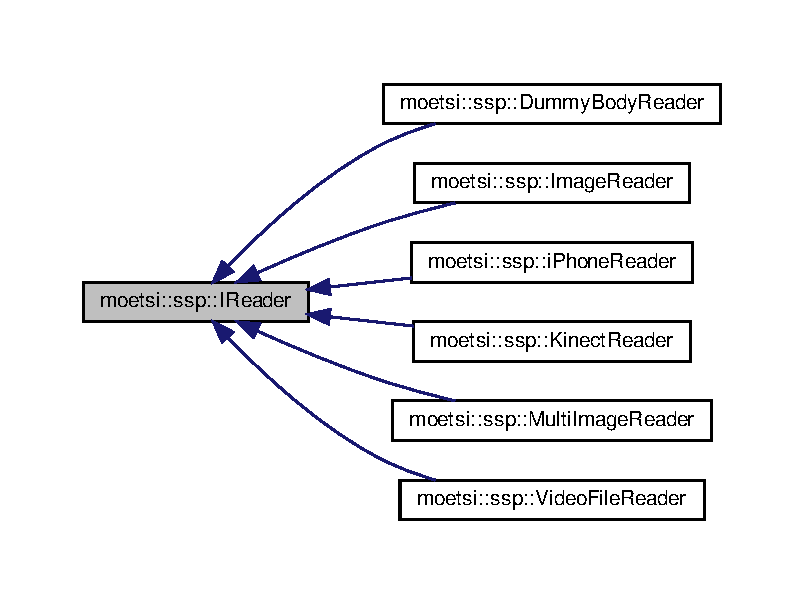
\includegraphics[width=350pt]{classmoetsi_1_1ssp_1_1IReader__inherit__graph}
\end{center}
\end{figure}
\subsection*{Public Member Functions}
\begin{DoxyCompactItemize}
\item 
\mbox{\Hypertarget{classmoetsi_1_1ssp_1_1IReader_ae1332862a7d81d99563f111ae36e142f}\label{classmoetsi_1_1ssp_1_1IReader_ae1332862a7d81d99563f111ae36e142f}} 
virtual \hyperlink{classmoetsi_1_1ssp_1_1IReader_ae1332862a7d81d99563f111ae36e142f}{$\sim$\+I\+Reader} ()
\begin{DoxyCompactList}\small\item\em Destructor. \end{DoxyCompactList}\item 
\mbox{\Hypertarget{classmoetsi_1_1ssp_1_1IReader_a357439182128e3911d77335c136035c0}\label{classmoetsi_1_1ssp_1_1IReader_a357439182128e3911d77335c136035c0}} 
virtual std\+::vector$<$ std\+::shared\+\_\+ptr$<$ \hyperlink{structmoetsi_1_1ssp_1_1FrameStruct}{Frame\+Struct} $>$ $>$ \hyperlink{classmoetsi_1_1ssp_1_1IReader_a357439182128e3911d77335c136035c0}{Get\+Current\+Frame} ()=0
\begin{DoxyCompactList}\small\item\em Get current frame data. \end{DoxyCompactList}\item 
virtual std\+::vector$<$ \hyperlink{namespacemoetsi_1_1ssp_a46efdfa2cd5a28ead465dcc8006b5a87}{Frame\+Type} $>$ \hyperlink{classmoetsi_1_1ssp_1_1IReader_a4116c1931fde7bd66133934ffdca1cce}{Get\+Type} ()=0
\begin{DoxyCompactList}\small\item\em Get frame types. \end{DoxyCompactList}\item 
virtual bool \hyperlink{classmoetsi_1_1ssp_1_1IReader_af9186ba41e136dc4ec3242b5dd55fa04}{Has\+Next\+Frame} ()=0
\begin{DoxyCompactList}\small\item\em Check if there is a next frame. \end{DoxyCompactList}\item 
\mbox{\Hypertarget{classmoetsi_1_1ssp_1_1IReader_a49e82a786cca55248e27e7fac8f97a17}\label{classmoetsi_1_1ssp_1_1IReader_a49e82a786cca55248e27e7fac8f97a17}} 
virtual void \hyperlink{classmoetsi_1_1ssp_1_1IReader_a49e82a786cca55248e27e7fac8f97a17}{Next\+Frame} ()=0
\begin{DoxyCompactList}\small\item\em Go to next frame. \end{DoxyCompactList}\item 
\mbox{\Hypertarget{classmoetsi_1_1ssp_1_1IReader_ad6e2ef78fc2466884aa877ecef54889d}\label{classmoetsi_1_1ssp_1_1IReader_ad6e2ef78fc2466884aa877ecef54889d}} 
virtual void \hyperlink{classmoetsi_1_1ssp_1_1IReader_ad6e2ef78fc2466884aa877ecef54889d}{Reset} ()=0
\begin{DoxyCompactList}\small\item\em Reset this reader. \end{DoxyCompactList}\item 
virtual void \hyperlink{classmoetsi_1_1ssp_1_1IReader_a6f1be3c06538992cca6d550bd9566681}{Go\+To\+Frame} (unsigned int frame\+\_\+id)=0
\begin{DoxyCompactList}\small\item\em Go to a given frame. \end{DoxyCompactList}\item 
virtual unsigned int \hyperlink{classmoetsi_1_1ssp_1_1IReader_ac292d83eb06dee277baaa06e281a562d}{Get\+Current\+Frame\+Id} ()=0
\begin{DoxyCompactList}\small\item\em Get current frame number. \end{DoxyCompactList}\item 
virtual unsigned int \hyperlink{classmoetsi_1_1ssp_1_1IReader_a9f6a8650ca290b011b8e5451eeae9f32}{Get\+Fps} ()=0
\begin{DoxyCompactList}\small\item\em Get indicative F\+PS in frame per second. \end{DoxyCompactList}\item 
\mbox{\Hypertarget{classmoetsi_1_1ssp_1_1IReader_ae1332862a7d81d99563f111ae36e142f}\label{classmoetsi_1_1ssp_1_1IReader_ae1332862a7d81d99563f111ae36e142f}} 
virtual \hyperlink{classmoetsi_1_1ssp_1_1IReader_ae1332862a7d81d99563f111ae36e142f}{$\sim$\+I\+Reader} ()
\begin{DoxyCompactList}\small\item\em Destructor. \end{DoxyCompactList}\item 
\mbox{\Hypertarget{classmoetsi_1_1ssp_1_1IReader_a357439182128e3911d77335c136035c0}\label{classmoetsi_1_1ssp_1_1IReader_a357439182128e3911d77335c136035c0}} 
virtual std\+::vector$<$ std\+::shared\+\_\+ptr$<$ \hyperlink{structmoetsi_1_1ssp_1_1FrameStruct}{Frame\+Struct} $>$ $>$ \hyperlink{classmoetsi_1_1ssp_1_1IReader_a357439182128e3911d77335c136035c0}{Get\+Current\+Frame} ()=0
\begin{DoxyCompactList}\small\item\em Get current frame data. \end{DoxyCompactList}\item 
virtual std\+::vector$<$ \hyperlink{namespacemoetsi_1_1ssp_a46efdfa2cd5a28ead465dcc8006b5a87}{Frame\+Type} $>$ \hyperlink{classmoetsi_1_1ssp_1_1IReader_a4116c1931fde7bd66133934ffdca1cce}{Get\+Type} ()=0
\begin{DoxyCompactList}\small\item\em Get frame types. \end{DoxyCompactList}\item 
virtual bool \hyperlink{classmoetsi_1_1ssp_1_1IReader_af9186ba41e136dc4ec3242b5dd55fa04}{Has\+Next\+Frame} ()=0
\begin{DoxyCompactList}\small\item\em Check if there is a next frame. \end{DoxyCompactList}\item 
\mbox{\Hypertarget{classmoetsi_1_1ssp_1_1IReader_a49e82a786cca55248e27e7fac8f97a17}\label{classmoetsi_1_1ssp_1_1IReader_a49e82a786cca55248e27e7fac8f97a17}} 
virtual void \hyperlink{classmoetsi_1_1ssp_1_1IReader_a49e82a786cca55248e27e7fac8f97a17}{Next\+Frame} ()=0
\begin{DoxyCompactList}\small\item\em Go to next frame. \end{DoxyCompactList}\item 
\mbox{\Hypertarget{classmoetsi_1_1ssp_1_1IReader_ad6e2ef78fc2466884aa877ecef54889d}\label{classmoetsi_1_1ssp_1_1IReader_ad6e2ef78fc2466884aa877ecef54889d}} 
virtual void \hyperlink{classmoetsi_1_1ssp_1_1IReader_ad6e2ef78fc2466884aa877ecef54889d}{Reset} ()=0
\begin{DoxyCompactList}\small\item\em Reset this reader. \end{DoxyCompactList}\item 
virtual void \hyperlink{classmoetsi_1_1ssp_1_1IReader_a6f1be3c06538992cca6d550bd9566681}{Go\+To\+Frame} (unsigned int frame\+\_\+id)=0
\begin{DoxyCompactList}\small\item\em Go to a given frame. \end{DoxyCompactList}\item 
virtual unsigned int \hyperlink{classmoetsi_1_1ssp_1_1IReader_ac292d83eb06dee277baaa06e281a562d}{Get\+Current\+Frame\+Id} ()=0
\begin{DoxyCompactList}\small\item\em Get current frame number. \end{DoxyCompactList}\item 
virtual unsigned int \hyperlink{classmoetsi_1_1ssp_1_1IReader_a9f6a8650ca290b011b8e5451eeae9f32}{Get\+Fps} ()=0
\begin{DoxyCompactList}\small\item\em Get indicative F\+PS in frame per second. \end{DoxyCompactList}\end{DoxyCompactItemize}


\subsection{Detailed Description}
S\+SP reader interface -\/ abstract class. 

\subsection{Member Function Documentation}
\mbox{\Hypertarget{classmoetsi_1_1ssp_1_1IReader_ac292d83eb06dee277baaa06e281a562d}\label{classmoetsi_1_1ssp_1_1IReader_ac292d83eb06dee277baaa06e281a562d}} 
\index{moetsi\+::ssp\+::\+I\+Reader@{moetsi\+::ssp\+::\+I\+Reader}!Get\+Current\+Frame\+Id@{Get\+Current\+Frame\+Id}}
\index{Get\+Current\+Frame\+Id@{Get\+Current\+Frame\+Id}!moetsi\+::ssp\+::\+I\+Reader@{moetsi\+::ssp\+::\+I\+Reader}}
\subsubsection{\texorpdfstring{Get\+Current\+Frame\+Id()}{GetCurrentFrameId()}\hspace{0.1cm}{\footnotesize\ttfamily [1/2]}}
{\footnotesize\ttfamily virtual unsigned int moetsi\+::ssp\+::\+I\+Reader\+::\+Get\+Current\+Frame\+Id (\begin{DoxyParamCaption}{ }\end{DoxyParamCaption})\hspace{0.3cm}{\ttfamily [pure virtual]}}



Get current frame number. 

\begin{DoxyReturn}{Returns}
current frame number. 
\end{DoxyReturn}


Implemented in \hyperlink{classmoetsi_1_1ssp_1_1KinectReader_aa17e268723c41bdad5082575decb28eb}{moetsi\+::ssp\+::\+Kinect\+Reader}, \hyperlink{classmoetsi_1_1ssp_1_1VideoFileReader_aef5c92da2645cddc7e4ffcfd34ad4b8a}{moetsi\+::ssp\+::\+Video\+File\+Reader}, \hyperlink{classmoetsi_1_1ssp_1_1ImageReader_a386125736df9f25e5c4312bb679ff031}{moetsi\+::ssp\+::\+Image\+Reader}, \hyperlink{classmoetsi_1_1ssp_1_1MultiImageReader_a994eea20e9682c2f4afc9303a34c76f3}{moetsi\+::ssp\+::\+Multi\+Image\+Reader}, and \hyperlink{classmoetsi_1_1ssp_1_1iPhoneReader_a78792c6319743aed3ef2afc96fe16485}{moetsi\+::ssp\+::i\+Phone\+Reader}.

\mbox{\Hypertarget{classmoetsi_1_1ssp_1_1IReader_ac292d83eb06dee277baaa06e281a562d}\label{classmoetsi_1_1ssp_1_1IReader_ac292d83eb06dee277baaa06e281a562d}} 
\index{moetsi\+::ssp\+::\+I\+Reader@{moetsi\+::ssp\+::\+I\+Reader}!Get\+Current\+Frame\+Id@{Get\+Current\+Frame\+Id}}
\index{Get\+Current\+Frame\+Id@{Get\+Current\+Frame\+Id}!moetsi\+::ssp\+::\+I\+Reader@{moetsi\+::ssp\+::\+I\+Reader}}
\subsubsection{\texorpdfstring{Get\+Current\+Frame\+Id()}{GetCurrentFrameId()}\hspace{0.1cm}{\footnotesize\ttfamily [2/2]}}
{\footnotesize\ttfamily virtual unsigned int moetsi\+::ssp\+::\+I\+Reader\+::\+Get\+Current\+Frame\+Id (\begin{DoxyParamCaption}{ }\end{DoxyParamCaption})\hspace{0.3cm}{\ttfamily [pure virtual]}}



Get current frame number. 

\begin{DoxyReturn}{Returns}
current frame number. 
\end{DoxyReturn}


Implemented in \hyperlink{classmoetsi_1_1ssp_1_1KinectReader_aa17e268723c41bdad5082575decb28eb}{moetsi\+::ssp\+::\+Kinect\+Reader}, \hyperlink{classmoetsi_1_1ssp_1_1VideoFileReader_aef5c92da2645cddc7e4ffcfd34ad4b8a}{moetsi\+::ssp\+::\+Video\+File\+Reader}, \hyperlink{classmoetsi_1_1ssp_1_1ImageReader_a386125736df9f25e5c4312bb679ff031}{moetsi\+::ssp\+::\+Image\+Reader}, \hyperlink{classmoetsi_1_1ssp_1_1MultiImageReader_a994eea20e9682c2f4afc9303a34c76f3}{moetsi\+::ssp\+::\+Multi\+Image\+Reader}, and \hyperlink{classmoetsi_1_1ssp_1_1iPhoneReader_a78792c6319743aed3ef2afc96fe16485}{moetsi\+::ssp\+::i\+Phone\+Reader}.

\mbox{\Hypertarget{classmoetsi_1_1ssp_1_1IReader_a9f6a8650ca290b011b8e5451eeae9f32}\label{classmoetsi_1_1ssp_1_1IReader_a9f6a8650ca290b011b8e5451eeae9f32}} 
\index{moetsi\+::ssp\+::\+I\+Reader@{moetsi\+::ssp\+::\+I\+Reader}!Get\+Fps@{Get\+Fps}}
\index{Get\+Fps@{Get\+Fps}!moetsi\+::ssp\+::\+I\+Reader@{moetsi\+::ssp\+::\+I\+Reader}}
\subsubsection{\texorpdfstring{Get\+Fps()}{GetFps()}\hspace{0.1cm}{\footnotesize\ttfamily [1/2]}}
{\footnotesize\ttfamily virtual unsigned int moetsi\+::ssp\+::\+I\+Reader\+::\+Get\+Fps (\begin{DoxyParamCaption}{ }\end{DoxyParamCaption})\hspace{0.3cm}{\ttfamily [pure virtual]}}



Get indicative F\+PS in frame per second. 

\begin{DoxyReturn}{Returns}
the F\+PS number 
\end{DoxyReturn}


Implemented in \hyperlink{classmoetsi_1_1ssp_1_1KinectReader_ac88c13693ce8e2e249438ac8de8a7b3c}{moetsi\+::ssp\+::\+Kinect\+Reader}, \hyperlink{classmoetsi_1_1ssp_1_1VideoFileReader_a83359ad82898acdb75240568b182247c}{moetsi\+::ssp\+::\+Video\+File\+Reader}, \hyperlink{classmoetsi_1_1ssp_1_1ImageReader_a86adfec8106c366aaf1ec63e2a7da156}{moetsi\+::ssp\+::\+Image\+Reader}, \hyperlink{classmoetsi_1_1ssp_1_1MultiImageReader_ad0a249af66f8e1a063c3e575fc1b94cb}{moetsi\+::ssp\+::\+Multi\+Image\+Reader}, and \hyperlink{classmoetsi_1_1ssp_1_1iPhoneReader_a4bb216847a6c2ed8eb5d31788a0b8477}{moetsi\+::ssp\+::i\+Phone\+Reader}.

\mbox{\Hypertarget{classmoetsi_1_1ssp_1_1IReader_a9f6a8650ca290b011b8e5451eeae9f32}\label{classmoetsi_1_1ssp_1_1IReader_a9f6a8650ca290b011b8e5451eeae9f32}} 
\index{moetsi\+::ssp\+::\+I\+Reader@{moetsi\+::ssp\+::\+I\+Reader}!Get\+Fps@{Get\+Fps}}
\index{Get\+Fps@{Get\+Fps}!moetsi\+::ssp\+::\+I\+Reader@{moetsi\+::ssp\+::\+I\+Reader}}
\subsubsection{\texorpdfstring{Get\+Fps()}{GetFps()}\hspace{0.1cm}{\footnotesize\ttfamily [2/2]}}
{\footnotesize\ttfamily virtual unsigned int moetsi\+::ssp\+::\+I\+Reader\+::\+Get\+Fps (\begin{DoxyParamCaption}{ }\end{DoxyParamCaption})\hspace{0.3cm}{\ttfamily [pure virtual]}}



Get indicative F\+PS in frame per second. 

\begin{DoxyReturn}{Returns}
the F\+PS number 
\end{DoxyReturn}


Implemented in \hyperlink{classmoetsi_1_1ssp_1_1KinectReader_ac88c13693ce8e2e249438ac8de8a7b3c}{moetsi\+::ssp\+::\+Kinect\+Reader}, \hyperlink{classmoetsi_1_1ssp_1_1VideoFileReader_a83359ad82898acdb75240568b182247c}{moetsi\+::ssp\+::\+Video\+File\+Reader}, \hyperlink{classmoetsi_1_1ssp_1_1ImageReader_a86adfec8106c366aaf1ec63e2a7da156}{moetsi\+::ssp\+::\+Image\+Reader}, \hyperlink{classmoetsi_1_1ssp_1_1MultiImageReader_ad0a249af66f8e1a063c3e575fc1b94cb}{moetsi\+::ssp\+::\+Multi\+Image\+Reader}, and \hyperlink{classmoetsi_1_1ssp_1_1iPhoneReader_a4bb216847a6c2ed8eb5d31788a0b8477}{moetsi\+::ssp\+::i\+Phone\+Reader}.

\mbox{\Hypertarget{classmoetsi_1_1ssp_1_1IReader_a4116c1931fde7bd66133934ffdca1cce}\label{classmoetsi_1_1ssp_1_1IReader_a4116c1931fde7bd66133934ffdca1cce}} 
\index{moetsi\+::ssp\+::\+I\+Reader@{moetsi\+::ssp\+::\+I\+Reader}!Get\+Type@{Get\+Type}}
\index{Get\+Type@{Get\+Type}!moetsi\+::ssp\+::\+I\+Reader@{moetsi\+::ssp\+::\+I\+Reader}}
\subsubsection{\texorpdfstring{Get\+Type()}{GetType()}\hspace{0.1cm}{\footnotesize\ttfamily [1/2]}}
{\footnotesize\ttfamily virtual std\+::vector$<$\hyperlink{namespacemoetsi_1_1ssp_a46efdfa2cd5a28ead465dcc8006b5a87}{Frame\+Type}$>$ moetsi\+::ssp\+::\+I\+Reader\+::\+Get\+Type (\begin{DoxyParamCaption}{ }\end{DoxyParamCaption})\hspace{0.3cm}{\ttfamily [pure virtual]}}



Get frame types. 

\begin{DoxyReturn}{Returns}
a vector of Frame\+Type, listing available data types 
\end{DoxyReturn}


Implemented in \hyperlink{classmoetsi_1_1ssp_1_1KinectReader_aef896aa686cbe1ea82dfc6aad46b6ff7}{moetsi\+::ssp\+::\+Kinect\+Reader}, \hyperlink{classmoetsi_1_1ssp_1_1VideoFileReader_a9d47af47299c5fccf766ac2d848a561b}{moetsi\+::ssp\+::\+Video\+File\+Reader}, \hyperlink{classmoetsi_1_1ssp_1_1ImageReader_af6f66957b6e3268c5336f4176c77fc73}{moetsi\+::ssp\+::\+Image\+Reader}, \hyperlink{classmoetsi_1_1ssp_1_1MultiImageReader_ad5f6cf0cfb1e64bcf569ab0bbfcce9d6}{moetsi\+::ssp\+::\+Multi\+Image\+Reader}, and \hyperlink{classmoetsi_1_1ssp_1_1iPhoneReader_a05d285ace85fc570bc2f453a0862ae56}{moetsi\+::ssp\+::i\+Phone\+Reader}.

\mbox{\Hypertarget{classmoetsi_1_1ssp_1_1IReader_a4116c1931fde7bd66133934ffdca1cce}\label{classmoetsi_1_1ssp_1_1IReader_a4116c1931fde7bd66133934ffdca1cce}} 
\index{moetsi\+::ssp\+::\+I\+Reader@{moetsi\+::ssp\+::\+I\+Reader}!Get\+Type@{Get\+Type}}
\index{Get\+Type@{Get\+Type}!moetsi\+::ssp\+::\+I\+Reader@{moetsi\+::ssp\+::\+I\+Reader}}
\subsubsection{\texorpdfstring{Get\+Type()}{GetType()}\hspace{0.1cm}{\footnotesize\ttfamily [2/2]}}
{\footnotesize\ttfamily virtual std\+::vector$<$\hyperlink{namespacemoetsi_1_1ssp_a46efdfa2cd5a28ead465dcc8006b5a87}{Frame\+Type}$>$ moetsi\+::ssp\+::\+I\+Reader\+::\+Get\+Type (\begin{DoxyParamCaption}{ }\end{DoxyParamCaption})\hspace{0.3cm}{\ttfamily [pure virtual]}}



Get frame types. 

\begin{DoxyReturn}{Returns}
a vector of Frame\+Type, listing available data types 
\end{DoxyReturn}


Implemented in \hyperlink{classmoetsi_1_1ssp_1_1KinectReader_aef896aa686cbe1ea82dfc6aad46b6ff7}{moetsi\+::ssp\+::\+Kinect\+Reader}, \hyperlink{classmoetsi_1_1ssp_1_1VideoFileReader_a9d47af47299c5fccf766ac2d848a561b}{moetsi\+::ssp\+::\+Video\+File\+Reader}, \hyperlink{classmoetsi_1_1ssp_1_1ImageReader_af6f66957b6e3268c5336f4176c77fc73}{moetsi\+::ssp\+::\+Image\+Reader}, \hyperlink{classmoetsi_1_1ssp_1_1MultiImageReader_ad5f6cf0cfb1e64bcf569ab0bbfcce9d6}{moetsi\+::ssp\+::\+Multi\+Image\+Reader}, and \hyperlink{classmoetsi_1_1ssp_1_1iPhoneReader_a05d285ace85fc570bc2f453a0862ae56}{moetsi\+::ssp\+::i\+Phone\+Reader}.

\mbox{\Hypertarget{classmoetsi_1_1ssp_1_1IReader_a6f1be3c06538992cca6d550bd9566681}\label{classmoetsi_1_1ssp_1_1IReader_a6f1be3c06538992cca6d550bd9566681}} 
\index{moetsi\+::ssp\+::\+I\+Reader@{moetsi\+::ssp\+::\+I\+Reader}!Go\+To\+Frame@{Go\+To\+Frame}}
\index{Go\+To\+Frame@{Go\+To\+Frame}!moetsi\+::ssp\+::\+I\+Reader@{moetsi\+::ssp\+::\+I\+Reader}}
\subsubsection{\texorpdfstring{Go\+To\+Frame()}{GoToFrame()}\hspace{0.1cm}{\footnotesize\ttfamily [1/2]}}
{\footnotesize\ttfamily virtual void moetsi\+::ssp\+::\+I\+Reader\+::\+Go\+To\+Frame (\begin{DoxyParamCaption}\item[{unsigned int}]{frame\+\_\+id }\end{DoxyParamCaption})\hspace{0.3cm}{\ttfamily [pure virtual]}}



Go to a given frame. 


\begin{DoxyParams}{Parameters}
{\em frame\+\_\+id} & target frame number \\
\hline
\end{DoxyParams}


Implemented in \hyperlink{classmoetsi_1_1ssp_1_1KinectReader_a315690c46e153a35d4ded1189e93af08}{moetsi\+::ssp\+::\+Kinect\+Reader}, \hyperlink{classmoetsi_1_1ssp_1_1VideoFileReader_ad98a532db8b1e2c3879df274b2efb082}{moetsi\+::ssp\+::\+Video\+File\+Reader}, \hyperlink{classmoetsi_1_1ssp_1_1ImageReader_a32eb88cc612e6920f4910e0803b0ce3c}{moetsi\+::ssp\+::\+Image\+Reader}, \hyperlink{classmoetsi_1_1ssp_1_1MultiImageReader_a7c552a1ad469660ea0a88b9ca85138ad}{moetsi\+::ssp\+::\+Multi\+Image\+Reader}, and \hyperlink{classmoetsi_1_1ssp_1_1iPhoneReader_a27b6dea97e4c4db8e4e749cc9e30e7ca}{moetsi\+::ssp\+::i\+Phone\+Reader}.

\mbox{\Hypertarget{classmoetsi_1_1ssp_1_1IReader_a6f1be3c06538992cca6d550bd9566681}\label{classmoetsi_1_1ssp_1_1IReader_a6f1be3c06538992cca6d550bd9566681}} 
\index{moetsi\+::ssp\+::\+I\+Reader@{moetsi\+::ssp\+::\+I\+Reader}!Go\+To\+Frame@{Go\+To\+Frame}}
\index{Go\+To\+Frame@{Go\+To\+Frame}!moetsi\+::ssp\+::\+I\+Reader@{moetsi\+::ssp\+::\+I\+Reader}}
\subsubsection{\texorpdfstring{Go\+To\+Frame()}{GoToFrame()}\hspace{0.1cm}{\footnotesize\ttfamily [2/2]}}
{\footnotesize\ttfamily virtual void moetsi\+::ssp\+::\+I\+Reader\+::\+Go\+To\+Frame (\begin{DoxyParamCaption}\item[{unsigned int}]{frame\+\_\+id }\end{DoxyParamCaption})\hspace{0.3cm}{\ttfamily [pure virtual]}}



Go to a given frame. 


\begin{DoxyParams}{Parameters}
{\em frame\+\_\+id} & target frame number \\
\hline
\end{DoxyParams}


Implemented in \hyperlink{classmoetsi_1_1ssp_1_1KinectReader_a315690c46e153a35d4ded1189e93af08}{moetsi\+::ssp\+::\+Kinect\+Reader}, \hyperlink{classmoetsi_1_1ssp_1_1VideoFileReader_ad98a532db8b1e2c3879df274b2efb082}{moetsi\+::ssp\+::\+Video\+File\+Reader}, \hyperlink{classmoetsi_1_1ssp_1_1ImageReader_a32eb88cc612e6920f4910e0803b0ce3c}{moetsi\+::ssp\+::\+Image\+Reader}, \hyperlink{classmoetsi_1_1ssp_1_1MultiImageReader_a7c552a1ad469660ea0a88b9ca85138ad}{moetsi\+::ssp\+::\+Multi\+Image\+Reader}, and \hyperlink{classmoetsi_1_1ssp_1_1iPhoneReader_a27b6dea97e4c4db8e4e749cc9e30e7ca}{moetsi\+::ssp\+::i\+Phone\+Reader}.

\mbox{\Hypertarget{classmoetsi_1_1ssp_1_1IReader_af9186ba41e136dc4ec3242b5dd55fa04}\label{classmoetsi_1_1ssp_1_1IReader_af9186ba41e136dc4ec3242b5dd55fa04}} 
\index{moetsi\+::ssp\+::\+I\+Reader@{moetsi\+::ssp\+::\+I\+Reader}!Has\+Next\+Frame@{Has\+Next\+Frame}}
\index{Has\+Next\+Frame@{Has\+Next\+Frame}!moetsi\+::ssp\+::\+I\+Reader@{moetsi\+::ssp\+::\+I\+Reader}}
\subsubsection{\texorpdfstring{Has\+Next\+Frame()}{HasNextFrame()}\hspace{0.1cm}{\footnotesize\ttfamily [1/2]}}
{\footnotesize\ttfamily virtual bool moetsi\+::ssp\+::\+I\+Reader\+::\+Has\+Next\+Frame (\begin{DoxyParamCaption}{ }\end{DoxyParamCaption})\hspace{0.3cm}{\ttfamily [pure virtual]}}



Check if there is a next frame. 

\begin{DoxyReturn}{Returns}
true if there is a next frame 
\end{DoxyReturn}


Implemented in \hyperlink{classmoetsi_1_1ssp_1_1KinectReader_a08934b6eff437142e482bb21780ca171}{moetsi\+::ssp\+::\+Kinect\+Reader}, \hyperlink{classmoetsi_1_1ssp_1_1VideoFileReader_ab5733b56b6d6dd7596eac9d914481c7e}{moetsi\+::ssp\+::\+Video\+File\+Reader}, \hyperlink{classmoetsi_1_1ssp_1_1ImageReader_ad8e87720ca0ec97de501f1070119b28d}{moetsi\+::ssp\+::\+Image\+Reader}, \hyperlink{classmoetsi_1_1ssp_1_1MultiImageReader_a04240c98d28d8949fca4ecdcb04f04f5}{moetsi\+::ssp\+::\+Multi\+Image\+Reader}, and \hyperlink{classmoetsi_1_1ssp_1_1iPhoneReader_a35ca55a03a9fb7b559f9381b11f53bfe}{moetsi\+::ssp\+::i\+Phone\+Reader}.

\mbox{\Hypertarget{classmoetsi_1_1ssp_1_1IReader_af9186ba41e136dc4ec3242b5dd55fa04}\label{classmoetsi_1_1ssp_1_1IReader_af9186ba41e136dc4ec3242b5dd55fa04}} 
\index{moetsi\+::ssp\+::\+I\+Reader@{moetsi\+::ssp\+::\+I\+Reader}!Has\+Next\+Frame@{Has\+Next\+Frame}}
\index{Has\+Next\+Frame@{Has\+Next\+Frame}!moetsi\+::ssp\+::\+I\+Reader@{moetsi\+::ssp\+::\+I\+Reader}}
\subsubsection{\texorpdfstring{Has\+Next\+Frame()}{HasNextFrame()}\hspace{0.1cm}{\footnotesize\ttfamily [2/2]}}
{\footnotesize\ttfamily virtual bool moetsi\+::ssp\+::\+I\+Reader\+::\+Has\+Next\+Frame (\begin{DoxyParamCaption}{ }\end{DoxyParamCaption})\hspace{0.3cm}{\ttfamily [pure virtual]}}



Check if there is a next frame. 

\begin{DoxyReturn}{Returns}
true if there is a next frame 
\end{DoxyReturn}


Implemented in \hyperlink{classmoetsi_1_1ssp_1_1KinectReader_a08934b6eff437142e482bb21780ca171}{moetsi\+::ssp\+::\+Kinect\+Reader}, \hyperlink{classmoetsi_1_1ssp_1_1VideoFileReader_ab5733b56b6d6dd7596eac9d914481c7e}{moetsi\+::ssp\+::\+Video\+File\+Reader}, \hyperlink{classmoetsi_1_1ssp_1_1ImageReader_ad8e87720ca0ec97de501f1070119b28d}{moetsi\+::ssp\+::\+Image\+Reader}, \hyperlink{classmoetsi_1_1ssp_1_1MultiImageReader_a04240c98d28d8949fca4ecdcb04f04f5}{moetsi\+::ssp\+::\+Multi\+Image\+Reader}, and \hyperlink{classmoetsi_1_1ssp_1_1iPhoneReader_a35ca55a03a9fb7b559f9381b11f53bfe}{moetsi\+::ssp\+::i\+Phone\+Reader}.



The documentation for this class was generated from the following file\+:\begin{DoxyCompactItemize}
\item 
include/readers/ireader.\+h\end{DoxyCompactItemize}

\hypertarget{classmoetsi_1_1ssp_1_1KinectReader}{}\section{moetsi\+:\+:ssp\+:\+:Kinect\+Reader Class Reference}
\label{classmoetsi_1_1ssp_1_1KinectReader}\index{moetsi\+::ssp\+::\+Kinect\+Reader@{moetsi\+::ssp\+::\+Kinect\+Reader}}


Inheritance diagram for moetsi\+:\+:ssp\+:\+:Kinect\+Reader\+:
\nopagebreak
\begin{figure}[H]
\begin{center}
\leavevmode
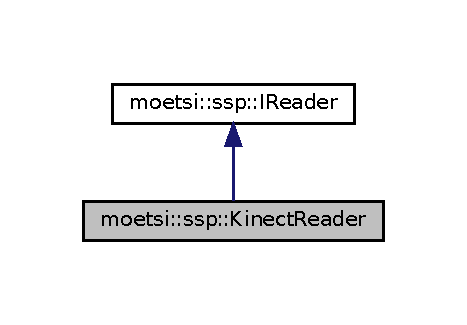
\includegraphics[width=213pt]{classmoetsi_1_1ssp_1_1KinectReader__inherit__graph}
\end{center}
\end{figure}


Collaboration diagram for moetsi\+:\+:ssp\+:\+:Kinect\+Reader\+:
\nopagebreak
\begin{figure}[H]
\begin{center}
\leavevmode
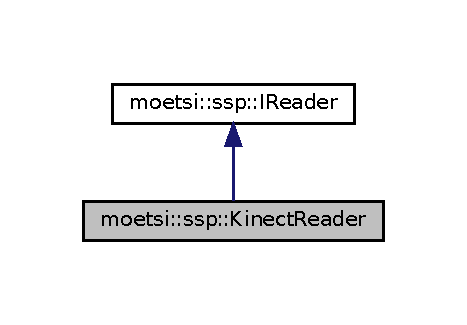
\includegraphics[width=213pt]{classmoetsi_1_1ssp_1_1KinectReader__coll__graph}
\end{center}
\end{figure}
\subsection*{Public Member Functions}
\begin{DoxyCompactItemize}
\item 
\mbox{\Hypertarget{classmoetsi_1_1ssp_1_1KinectReader_af992a9575612d1919ce9cf70b450e2e9}\label{classmoetsi_1_1ssp_1_1KinectReader_af992a9575612d1919ce9cf70b450e2e9}} 
{\bfseries Kinect\+Reader} (uint8\+\_\+t device\+\_\+index, \hyperlink{structmoetsi_1_1ssp_1_1ExtendedAzureConfig}{Extended\+Azure\+Config} device\+\_\+config)
\item 
\mbox{\Hypertarget{classmoetsi_1_1ssp_1_1KinectReader_a7f0d8f5d643ebeff0589eeb8af5b9a9e}\label{classmoetsi_1_1ssp_1_1KinectReader_a7f0d8f5d643ebeff0589eeb8af5b9a9e}} 
virtual std\+::vector$<$ std\+::shared\+\_\+ptr$<$ \hyperlink{structmoetsi_1_1ssp_1_1FrameStruct}{Frame\+Struct} $>$ $>$ \hyperlink{classmoetsi_1_1ssp_1_1KinectReader_a7f0d8f5d643ebeff0589eeb8af5b9a9e}{Get\+Current\+Frame} ()
\begin{DoxyCompactList}\small\item\em Get current frame data. \end{DoxyCompactList}\item 
virtual std\+::vector$<$ \hyperlink{namespacemoetsi_1_1ssp_a46efdfa2cd5a28ead465dcc8006b5a87}{Frame\+Type} $>$ \hyperlink{classmoetsi_1_1ssp_1_1KinectReader_aef896aa686cbe1ea82dfc6aad46b6ff7}{Get\+Type} ()
\begin{DoxyCompactList}\small\item\em Get frame types. \end{DoxyCompactList}\item 
virtual bool \hyperlink{classmoetsi_1_1ssp_1_1KinectReader_a08934b6eff437142e482bb21780ca171}{Has\+Next\+Frame} ()
\begin{DoxyCompactList}\small\item\em Check if there is a next frame. \end{DoxyCompactList}\item 
\mbox{\Hypertarget{classmoetsi_1_1ssp_1_1KinectReader_a8495eb28b3893281c1d4bbd5ba9f9739}\label{classmoetsi_1_1ssp_1_1KinectReader_a8495eb28b3893281c1d4bbd5ba9f9739}} 
virtual void \hyperlink{classmoetsi_1_1ssp_1_1KinectReader_a8495eb28b3893281c1d4bbd5ba9f9739}{Next\+Frame} ()
\begin{DoxyCompactList}\small\item\em Go to next frame. \end{DoxyCompactList}\item 
\mbox{\Hypertarget{classmoetsi_1_1ssp_1_1KinectReader_a0ad8f7b57ef04554e41a66db797c000e}\label{classmoetsi_1_1ssp_1_1KinectReader_a0ad8f7b57ef04554e41a66db797c000e}} 
virtual void \hyperlink{classmoetsi_1_1ssp_1_1KinectReader_a0ad8f7b57ef04554e41a66db797c000e}{Reset} ()
\begin{DoxyCompactList}\small\item\em Reset this reader. \end{DoxyCompactList}\item 
virtual void \hyperlink{classmoetsi_1_1ssp_1_1KinectReader_a315690c46e153a35d4ded1189e93af08}{Go\+To\+Frame} (unsigned int frame\+\_\+id)
\begin{DoxyCompactList}\small\item\em Go to a given frame. \end{DoxyCompactList}\item 
virtual unsigned int \hyperlink{classmoetsi_1_1ssp_1_1KinectReader_aa17e268723c41bdad5082575decb28eb}{Get\+Current\+Frame\+Id} ()
\begin{DoxyCompactList}\small\item\em Get current frame number. \end{DoxyCompactList}\item 
virtual unsigned int \hyperlink{classmoetsi_1_1ssp_1_1KinectReader_ac88c13693ce8e2e249438ac8de8a7b3c}{Get\+Fps} ()
\begin{DoxyCompactList}\small\item\em Get indicative F\+PS in frame per second. \end{DoxyCompactList}\end{DoxyCompactItemize}


\subsection{Member Function Documentation}
\mbox{\Hypertarget{classmoetsi_1_1ssp_1_1KinectReader_aa17e268723c41bdad5082575decb28eb}\label{classmoetsi_1_1ssp_1_1KinectReader_aa17e268723c41bdad5082575decb28eb}} 
\index{moetsi\+::ssp\+::\+Kinect\+Reader@{moetsi\+::ssp\+::\+Kinect\+Reader}!Get\+Current\+Frame\+Id@{Get\+Current\+Frame\+Id}}
\index{Get\+Current\+Frame\+Id@{Get\+Current\+Frame\+Id}!moetsi\+::ssp\+::\+Kinect\+Reader@{moetsi\+::ssp\+::\+Kinect\+Reader}}
\subsubsection{\texorpdfstring{Get\+Current\+Frame\+Id()}{GetCurrentFrameId()}}
{\footnotesize\ttfamily unsigned int moetsi\+::ssp\+::\+Kinect\+Reader\+::\+Get\+Current\+Frame\+Id (\begin{DoxyParamCaption}{ }\end{DoxyParamCaption})\hspace{0.3cm}{\ttfamily [virtual]}}



Get current frame number. 

\begin{DoxyReturn}{Returns}
current frame number. 
\end{DoxyReturn}


Implements \hyperlink{classmoetsi_1_1ssp_1_1IReader_ac292d83eb06dee277baaa06e281a562d}{moetsi\+::ssp\+::\+I\+Reader}.

\mbox{\Hypertarget{classmoetsi_1_1ssp_1_1KinectReader_ac88c13693ce8e2e249438ac8de8a7b3c}\label{classmoetsi_1_1ssp_1_1KinectReader_ac88c13693ce8e2e249438ac8de8a7b3c}} 
\index{moetsi\+::ssp\+::\+Kinect\+Reader@{moetsi\+::ssp\+::\+Kinect\+Reader}!Get\+Fps@{Get\+Fps}}
\index{Get\+Fps@{Get\+Fps}!moetsi\+::ssp\+::\+Kinect\+Reader@{moetsi\+::ssp\+::\+Kinect\+Reader}}
\subsubsection{\texorpdfstring{Get\+Fps()}{GetFps()}}
{\footnotesize\ttfamily unsigned int moetsi\+::ssp\+::\+Kinect\+Reader\+::\+Get\+Fps (\begin{DoxyParamCaption}{ }\end{DoxyParamCaption})\hspace{0.3cm}{\ttfamily [virtual]}}



Get indicative F\+PS in frame per second. 

\begin{DoxyReturn}{Returns}
the F\+PS number 
\end{DoxyReturn}


Implements \hyperlink{classmoetsi_1_1ssp_1_1IReader_a9f6a8650ca290b011b8e5451eeae9f32}{moetsi\+::ssp\+::\+I\+Reader}.

\mbox{\Hypertarget{classmoetsi_1_1ssp_1_1KinectReader_aef896aa686cbe1ea82dfc6aad46b6ff7}\label{classmoetsi_1_1ssp_1_1KinectReader_aef896aa686cbe1ea82dfc6aad46b6ff7}} 
\index{moetsi\+::ssp\+::\+Kinect\+Reader@{moetsi\+::ssp\+::\+Kinect\+Reader}!Get\+Type@{Get\+Type}}
\index{Get\+Type@{Get\+Type}!moetsi\+::ssp\+::\+Kinect\+Reader@{moetsi\+::ssp\+::\+Kinect\+Reader}}
\subsubsection{\texorpdfstring{Get\+Type()}{GetType()}}
{\footnotesize\ttfamily std\+::vector$<$ \hyperlink{namespacemoetsi_1_1ssp_a46efdfa2cd5a28ead465dcc8006b5a87}{Frame\+Type} $>$ moetsi\+::ssp\+::\+Kinect\+Reader\+::\+Get\+Type (\begin{DoxyParamCaption}{ }\end{DoxyParamCaption})\hspace{0.3cm}{\ttfamily [virtual]}}



Get frame types. 

\begin{DoxyReturn}{Returns}
a vector of Frame\+Type, listing available data types 
\end{DoxyReturn}


Implements \hyperlink{classmoetsi_1_1ssp_1_1IReader_a4116c1931fde7bd66133934ffdca1cce}{moetsi\+::ssp\+::\+I\+Reader}.

\mbox{\Hypertarget{classmoetsi_1_1ssp_1_1KinectReader_a315690c46e153a35d4ded1189e93af08}\label{classmoetsi_1_1ssp_1_1KinectReader_a315690c46e153a35d4ded1189e93af08}} 
\index{moetsi\+::ssp\+::\+Kinect\+Reader@{moetsi\+::ssp\+::\+Kinect\+Reader}!Go\+To\+Frame@{Go\+To\+Frame}}
\index{Go\+To\+Frame@{Go\+To\+Frame}!moetsi\+::ssp\+::\+Kinect\+Reader@{moetsi\+::ssp\+::\+Kinect\+Reader}}
\subsubsection{\texorpdfstring{Go\+To\+Frame()}{GoToFrame()}}
{\footnotesize\ttfamily void moetsi\+::ssp\+::\+Kinect\+Reader\+::\+Go\+To\+Frame (\begin{DoxyParamCaption}\item[{unsigned int}]{frame\+\_\+id }\end{DoxyParamCaption})\hspace{0.3cm}{\ttfamily [virtual]}}



Go to a given frame. 


\begin{DoxyParams}{Parameters}
{\em frame\+\_\+id} & target frame number \\
\hline
\end{DoxyParams}


Implements \hyperlink{classmoetsi_1_1ssp_1_1IReader_a6f1be3c06538992cca6d550bd9566681}{moetsi\+::ssp\+::\+I\+Reader}.

\mbox{\Hypertarget{classmoetsi_1_1ssp_1_1KinectReader_a08934b6eff437142e482bb21780ca171}\label{classmoetsi_1_1ssp_1_1KinectReader_a08934b6eff437142e482bb21780ca171}} 
\index{moetsi\+::ssp\+::\+Kinect\+Reader@{moetsi\+::ssp\+::\+Kinect\+Reader}!Has\+Next\+Frame@{Has\+Next\+Frame}}
\index{Has\+Next\+Frame@{Has\+Next\+Frame}!moetsi\+::ssp\+::\+Kinect\+Reader@{moetsi\+::ssp\+::\+Kinect\+Reader}}
\subsubsection{\texorpdfstring{Has\+Next\+Frame()}{HasNextFrame()}}
{\footnotesize\ttfamily bool moetsi\+::ssp\+::\+Kinect\+Reader\+::\+Has\+Next\+Frame (\begin{DoxyParamCaption}{ }\end{DoxyParamCaption})\hspace{0.3cm}{\ttfamily [virtual]}}



Check if there is a next frame. 

\begin{DoxyReturn}{Returns}
true if there is a next frame 
\end{DoxyReturn}


Implements \hyperlink{classmoetsi_1_1ssp_1_1IReader_af9186ba41e136dc4ec3242b5dd55fa04}{moetsi\+::ssp\+::\+I\+Reader}.



The documentation for this class was generated from the following files\+:\begin{DoxyCompactItemize}
\item 
\hyperlink{kinect__reader_8h}{kinect\+\_\+reader.\+h}\item 
\hyperlink{kinect__reader_8cc}{kinect\+\_\+reader.\+cc}\end{DoxyCompactItemize}

\hypertarget{classmoetsi_1_1ssp_1_1LibAvDecoder}{}\doxysection{moetsi\+::ssp\+::Lib\+Av\+Decoder Class Reference}
\label{classmoetsi_1_1ssp_1_1LibAvDecoder}\index{moetsi::ssp::LibAvDecoder@{moetsi::ssp::LibAvDecoder}}


AV (Jpeg/\+Mpeg) decoder.  




{\ttfamily \#include $<$libav\+\_\+decoder.\+h$>$}



Inheritance diagram for moetsi\+::ssp\+::Lib\+Av\+Decoder\+:
\nopagebreak
\begin{figure}[H]
\begin{center}
\leavevmode
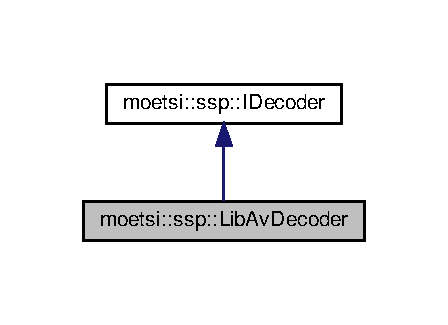
\includegraphics[width=226pt]{classmoetsi_1_1ssp_1_1LibAvDecoder__inherit__graph}
\end{center}
\end{figure}


Collaboration diagram for moetsi\+::ssp\+::Lib\+Av\+Decoder\+:
\nopagebreak
\begin{figure}[H]
\begin{center}
\leavevmode
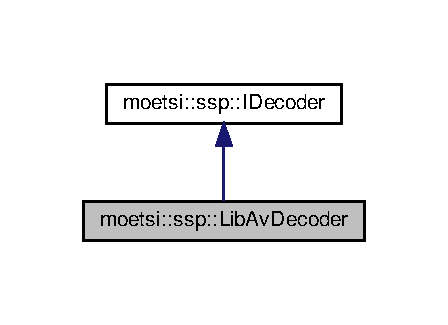
\includegraphics[width=226pt]{classmoetsi_1_1ssp_1_1LibAvDecoder__coll__graph}
\end{center}
\end{figure}
\doxysubsection*{Public Member Functions}
\begin{DoxyCompactItemize}
\item 
\mbox{\Hypertarget{classmoetsi_1_1ssp_1_1LibAvDecoder_a68174e3bd10e03eaabee437826399b64}\label{classmoetsi_1_1ssp_1_1LibAvDecoder_a68174e3bd10e03eaabee437826399b64}} 
\mbox{\hyperlink{classmoetsi_1_1ssp_1_1LibAvDecoder_a68174e3bd10e03eaabee437826399b64}{Lib\+Av\+Decoder}} ()
\begin{DoxyCompactList}\small\item\em constructor \end{DoxyCompactList}\item 
\mbox{\Hypertarget{classmoetsi_1_1ssp_1_1LibAvDecoder_a1aafd7da5bdd011aae77075b71e52f51}\label{classmoetsi_1_1ssp_1_1LibAvDecoder_a1aafd7da5bdd011aae77075b71e52f51}} 
\mbox{\hyperlink{classmoetsi_1_1ssp_1_1LibAvDecoder_a1aafd7da5bdd011aae77075b71e52f51}{$\sim$\+Lib\+Av\+Decoder}} ()
\begin{DoxyCompactList}\small\item\em destructor \end{DoxyCompactList}\item 
void \mbox{\hyperlink{classmoetsi_1_1ssp_1_1LibAvDecoder_a631ce4158ab4f456a26951674f96a803}{Init}} (A\+V\+Codec\+Parameters $\ast$codec\+\_\+parameters)
\begin{DoxyCompactList}\small\item\em Initialize. \end{DoxyCompactList}\item 
cv\+::\+Mat \mbox{\hyperlink{classmoetsi_1_1ssp_1_1LibAvDecoder_a4206a4581de1b93d6c6a0835e8cf4ac8}{Decode}} (\mbox{\hyperlink{structmoetsi_1_1ssp_1_1FrameStruct}{Frame\+Struct}} \&frame\+\_\+struct)
\begin{DoxyCompactList}\small\item\em Extract an opencv image from a \mbox{\hyperlink{structmoetsi_1_1ssp_1_1FrameStruct}{Frame\+Struct}}. \end{DoxyCompactList}\item 
A\+V\+Frame\+SharedP \mbox{\hyperlink{classmoetsi_1_1ssp_1_1LibAvDecoder_a41c94bd7fa9576902ea0a6e95e59d93e}{Decode\+Frame}} (\mbox{\hyperlink{structmoetsi_1_1ssp_1_1FrameStruct}{Frame\+Struct}} \&frame\+\_\+struct)
\begin{DoxyCompactList}\small\item\em Decode frame to libav A\+V\+Frame structure. \end{DoxyCompactList}\end{DoxyCompactItemize}


\doxysubsection{Detailed Description}
AV (Jpeg/\+Mpeg) decoder. 

\doxysubsection{Member Function Documentation}
\mbox{\Hypertarget{classmoetsi_1_1ssp_1_1LibAvDecoder_a4206a4581de1b93d6c6a0835e8cf4ac8}\label{classmoetsi_1_1ssp_1_1LibAvDecoder_a4206a4581de1b93d6c6a0835e8cf4ac8}} 
\index{moetsi::ssp::LibAvDecoder@{moetsi::ssp::LibAvDecoder}!Decode@{Decode}}
\index{Decode@{Decode}!moetsi::ssp::LibAvDecoder@{moetsi::ssp::LibAvDecoder}}
\doxysubsubsection{\texorpdfstring{Decode()}{Decode()}}
{\footnotesize\ttfamily cv\+::\+Mat moetsi\+::ssp\+::\+Lib\+Av\+Decoder\+::\+Decode (\begin{DoxyParamCaption}\item[{\mbox{\hyperlink{structmoetsi_1_1ssp_1_1FrameStruct}{Frame\+Struct}} \&}]{frame\+\_\+struct }\end{DoxyParamCaption})\hspace{0.3cm}{\ttfamily [virtual]}}



Extract an opencv image from a \mbox{\hyperlink{structmoetsi_1_1ssp_1_1FrameStruct}{Frame\+Struct}}. 


\begin{DoxyParams}{Parameters}
{\em data} & \mbox{\hyperlink{structmoetsi_1_1ssp_1_1FrameStruct}{Frame\+Struct}} \\
\hline
\end{DoxyParams}
\begin{DoxyReturn}{Returns}
Open\+CV matrix/image 
\end{DoxyReturn}


Implements \mbox{\hyperlink{classmoetsi_1_1ssp_1_1IDecoder_a1c06604dc4107d3668a4e791c13cc063}{moetsi\+::ssp\+::\+I\+Decoder}}.

\mbox{\Hypertarget{classmoetsi_1_1ssp_1_1LibAvDecoder_a41c94bd7fa9576902ea0a6e95e59d93e}\label{classmoetsi_1_1ssp_1_1LibAvDecoder_a41c94bd7fa9576902ea0a6e95e59d93e}} 
\index{moetsi::ssp::LibAvDecoder@{moetsi::ssp::LibAvDecoder}!DecodeFrame@{DecodeFrame}}
\index{DecodeFrame@{DecodeFrame}!moetsi::ssp::LibAvDecoder@{moetsi::ssp::LibAvDecoder}}
\doxysubsubsection{\texorpdfstring{DecodeFrame()}{DecodeFrame()}}
{\footnotesize\ttfamily A\+V\+Frame\+SharedP moetsi\+::ssp\+::\+Lib\+Av\+Decoder\+::\+Decode\+Frame (\begin{DoxyParamCaption}\item[{\mbox{\hyperlink{structmoetsi_1_1ssp_1_1FrameStruct}{Frame\+Struct}} \&}]{frame\+\_\+struct }\end{DoxyParamCaption})}



Decode frame to libav A\+V\+Frame structure. 


\begin{DoxyParams}{Parameters}
{\em frame\+\_\+struct} & S\+SP \mbox{\hyperlink{structmoetsi_1_1ssp_1_1FrameStruct}{Frame\+Struct}} \\
\hline
\end{DoxyParams}
\begin{DoxyReturn}{Returns}
Libav A\+V\+Frame structure 
\end{DoxyReturn}
\mbox{\Hypertarget{classmoetsi_1_1ssp_1_1LibAvDecoder_a631ce4158ab4f456a26951674f96a803}\label{classmoetsi_1_1ssp_1_1LibAvDecoder_a631ce4158ab4f456a26951674f96a803}} 
\index{moetsi::ssp::LibAvDecoder@{moetsi::ssp::LibAvDecoder}!Init@{Init}}
\index{Init@{Init}!moetsi::ssp::LibAvDecoder@{moetsi::ssp::LibAvDecoder}}
\doxysubsubsection{\texorpdfstring{Init()}{Init()}}
{\footnotesize\ttfamily void moetsi\+::ssp\+::\+Lib\+Av\+Decoder\+::\+Init (\begin{DoxyParamCaption}\item[{A\+V\+Codec\+Parameters $\ast$}]{codec\+\_\+parameters }\end{DoxyParamCaption})}



Initialize. 


\begin{DoxyParams}{Parameters}
{\em codec\+\_\+parameters} & parameters \\
\hline
\end{DoxyParams}


The documentation for this class was generated from the following files\+:\begin{DoxyCompactItemize}
\item 
\mbox{\hyperlink{libav__decoder_8h}{libav\+\_\+decoder.\+h}}\item 
\mbox{\hyperlink{libav__decoder_8cc}{libav\+\_\+decoder.\+cc}}\end{DoxyCompactItemize}

\hypertarget{classmoetsi_1_1ssp_1_1LibAvEncoder}{}\doxysection{moetsi\+::ssp\+::Lib\+Av\+Encoder Class Reference}
\label{classmoetsi_1_1ssp_1_1LibAvEncoder}\index{moetsi::ssp::LibAvEncoder@{moetsi::ssp::LibAvEncoder}}


Lib\+AV encoder for Jpeg/\+Mpeg.  




{\ttfamily \#include $<$libav\+\_\+encoder.\+h$>$}



Inheritance diagram for moetsi\+::ssp\+::Lib\+Av\+Encoder\+:
\nopagebreak
\begin{figure}[H]
\begin{center}
\leavevmode
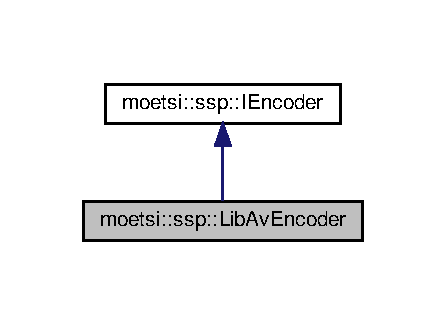
\includegraphics[width=224pt]{classmoetsi_1_1ssp_1_1LibAvEncoder__inherit__graph}
\end{center}
\end{figure}


Collaboration diagram for moetsi\+::ssp\+::Lib\+Av\+Encoder\+:
\nopagebreak
\begin{figure}[H]
\begin{center}
\leavevmode
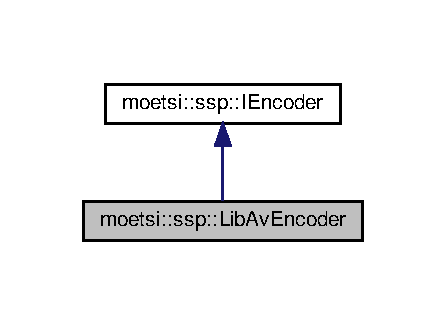
\includegraphics[width=224pt]{classmoetsi_1_1ssp_1_1LibAvEncoder__coll__graph}
\end{center}
\end{figure}
\doxysubsection*{Public Member Functions}
\begin{DoxyCompactItemize}
\item 
\mbox{\hyperlink{classmoetsi_1_1ssp_1_1LibAvEncoder_a92b5b4c1f7da0a5cbf30bbf4fe7c89d4}{Lib\+Av\+Encoder}} (std\+::string codec\+\_\+parameters\+\_\+file, unsigned int fps)
\begin{DoxyCompactList}\small\item\em Constructor. \end{DoxyCompactList}\item 
\mbox{\hyperlink{classmoetsi_1_1ssp_1_1LibAvEncoder_a2d5ec3b4a92f7b9378fd397624bd4ea4}{Lib\+Av\+Encoder}} (Y\+A\+M\+L\+::\+Node \&\+\_\+codec\+\_\+parameters, unsigned int fps)
\begin{DoxyCompactList}\small\item\em Constructor. \end{DoxyCompactList}\item 
\mbox{\Hypertarget{classmoetsi_1_1ssp_1_1LibAvEncoder_aad54739bf358507ec23b25d44bb3ad4d}\label{classmoetsi_1_1ssp_1_1LibAvEncoder_aad54739bf358507ec23b25d44bb3ad4d}} 
virtual \mbox{\hyperlink{classmoetsi_1_1ssp_1_1LibAvEncoder_aad54739bf358507ec23b25d44bb3ad4d}{$\sim$\+Lib\+Av\+Encoder}} ()
\begin{DoxyCompactList}\small\item\em Destructor. \end{DoxyCompactList}\item 
virtual void \mbox{\hyperlink{classmoetsi_1_1ssp_1_1LibAvEncoder_a931327f154e0da63fdfed73cf317d688}{Add\+Frame\+Struct}} (std\+::shared\+\_\+ptr$<$ \mbox{\hyperlink{structmoetsi_1_1ssp_1_1FrameStruct}{Frame\+Struct}} $>$ \&frame\+\_\+struct)
\begin{DoxyCompactList}\small\item\em Add a frame struct. \end{DoxyCompactList}\item 
\mbox{\Hypertarget{classmoetsi_1_1ssp_1_1LibAvEncoder_acf5e6e2f172d24778c7942c8cd37330b}\label{classmoetsi_1_1ssp_1_1LibAvEncoder_acf5e6e2f172d24778c7942c8cd37330b}} 
virtual void \mbox{\hyperlink{classmoetsi_1_1ssp_1_1LibAvEncoder_acf5e6e2f172d24778c7942c8cd37330b}{Next\+Packet}} ()
\begin{DoxyCompactList}\small\item\em Go to next packet. \end{DoxyCompactList}\item 
virtual bool \mbox{\hyperlink{classmoetsi_1_1ssp_1_1LibAvEncoder_a306c0935fa37bd35ddfeb8290289e927}{Has\+Next\+Packet}} ()
\begin{DoxyCompactList}\small\item\em Check if there is a next packet. \end{DoxyCompactList}\item 
virtual std\+::shared\+\_\+ptr$<$ \mbox{\hyperlink{structmoetsi_1_1ssp_1_1FrameStruct}{Frame\+Struct}} $>$ \mbox{\hyperlink{classmoetsi_1_1ssp_1_1LibAvEncoder_aedb37703d73b55f1389a122d2ecbe923}{Current\+Frame\+Encoded}} ()
\begin{DoxyCompactList}\small\item\em Get current encoded frame. \end{DoxyCompactList}\item 
virtual std\+::shared\+\_\+ptr$<$ \mbox{\hyperlink{structmoetsi_1_1ssp_1_1FrameStruct}{Frame\+Struct}} $>$ \mbox{\hyperlink{classmoetsi_1_1ssp_1_1LibAvEncoder_a249c65ad557f438d6856e875f01a1947}{Current\+Frame\+Original}} ()
\begin{DoxyCompactList}\small\item\em Get current frame in its original format. \end{DoxyCompactList}\item 
virtual std\+::shared\+\_\+ptr$<$ \mbox{\hyperlink{structmoetsi_1_1ssp_1_1CodecParamsStruct}{Codec\+Params\+Struct}} $>$ \mbox{\hyperlink{classmoetsi_1_1ssp_1_1LibAvEncoder_a2ff6afafbb5da48e900d34d70a46d00c}{Get\+Codec\+Params\+Struct}} ()
\begin{DoxyCompactList}\small\item\em Get codec parameters. \end{DoxyCompactList}\item 
virtual unsigned int \mbox{\hyperlink{classmoetsi_1_1ssp_1_1LibAvEncoder_ae21f81cb967359132183a29e04307933}{Get\+Fps}} ()
\begin{DoxyCompactList}\small\item\em Get F\+PS. \end{DoxyCompactList}\end{DoxyCompactItemize}


\doxysubsection{Detailed Description}
Lib\+AV encoder for Jpeg/\+Mpeg. 

\doxysubsection{Constructor \& Destructor Documentation}
\mbox{\Hypertarget{classmoetsi_1_1ssp_1_1LibAvEncoder_a92b5b4c1f7da0a5cbf30bbf4fe7c89d4}\label{classmoetsi_1_1ssp_1_1LibAvEncoder_a92b5b4c1f7da0a5cbf30bbf4fe7c89d4}} 
\index{moetsi::ssp::LibAvEncoder@{moetsi::ssp::LibAvEncoder}!LibAvEncoder@{LibAvEncoder}}
\index{LibAvEncoder@{LibAvEncoder}!moetsi::ssp::LibAvEncoder@{moetsi::ssp::LibAvEncoder}}
\doxysubsubsection{\texorpdfstring{LibAvEncoder()}{LibAvEncoder()}\hspace{0.1cm}{\footnotesize\ttfamily [1/2]}}
{\footnotesize\ttfamily moetsi\+::ssp\+::\+Lib\+Av\+Encoder\+::\+Lib\+Av\+Encoder (\begin{DoxyParamCaption}\item[{std\+::string}]{codec\+\_\+parameters\+\_\+file,  }\item[{unsigned int}]{fps }\end{DoxyParamCaption})}



Constructor. 


\begin{DoxyParams}{Parameters}
{\em codec\+\_\+parameters\+\_\+file} & File with codec parameters \\
\hline
{\em fps} & Frame per second \\
\hline
\end{DoxyParams}
\mbox{\Hypertarget{classmoetsi_1_1ssp_1_1LibAvEncoder_a2d5ec3b4a92f7b9378fd397624bd4ea4}\label{classmoetsi_1_1ssp_1_1LibAvEncoder_a2d5ec3b4a92f7b9378fd397624bd4ea4}} 
\index{moetsi::ssp::LibAvEncoder@{moetsi::ssp::LibAvEncoder}!LibAvEncoder@{LibAvEncoder}}
\index{LibAvEncoder@{LibAvEncoder}!moetsi::ssp::LibAvEncoder@{moetsi::ssp::LibAvEncoder}}
\doxysubsubsection{\texorpdfstring{LibAvEncoder()}{LibAvEncoder()}\hspace{0.1cm}{\footnotesize\ttfamily [2/2]}}
{\footnotesize\ttfamily moetsi\+::ssp\+::\+Lib\+Av\+Encoder\+::\+Lib\+Av\+Encoder (\begin{DoxyParamCaption}\item[{Y\+A\+M\+L\+::\+Node \&}]{\+\_\+codec\+\_\+parameters,  }\item[{unsigned int}]{fps }\end{DoxyParamCaption})}



Constructor. 


\begin{DoxyParams}{Parameters}
{\em \+\_\+codec\+\_\+parameters} & Yaml codec parameters \\
\hline
{\em fps} & Frame per second \\
\hline
\end{DoxyParams}


\doxysubsection{Member Function Documentation}
\mbox{\Hypertarget{classmoetsi_1_1ssp_1_1LibAvEncoder_a931327f154e0da63fdfed73cf317d688}\label{classmoetsi_1_1ssp_1_1LibAvEncoder_a931327f154e0da63fdfed73cf317d688}} 
\index{moetsi::ssp::LibAvEncoder@{moetsi::ssp::LibAvEncoder}!AddFrameStruct@{AddFrameStruct}}
\index{AddFrameStruct@{AddFrameStruct}!moetsi::ssp::LibAvEncoder@{moetsi::ssp::LibAvEncoder}}
\doxysubsubsection{\texorpdfstring{AddFrameStruct()}{AddFrameStruct()}}
{\footnotesize\ttfamily void moetsi\+::ssp\+::\+Lib\+Av\+Encoder\+::\+Add\+Frame\+Struct (\begin{DoxyParamCaption}\item[{std\+::shared\+\_\+ptr$<$ \mbox{\hyperlink{structmoetsi_1_1ssp_1_1FrameStruct}{Frame\+Struct}} $>$ \&}]{frame\+\_\+struct }\end{DoxyParamCaption})\hspace{0.3cm}{\ttfamily [virtual]}}



Add a frame struct. 


\begin{DoxyParams}{Parameters}
{\em frame\+\_\+struct} & \mbox{\hyperlink{structmoetsi_1_1ssp_1_1FrameStruct}{Frame\+Struct}} to add \\
\hline
\end{DoxyParams}


Implements \mbox{\hyperlink{classmoetsi_1_1ssp_1_1IEncoder_a8c223ec82fdd30ee8ee75157306054ec}{moetsi\+::ssp\+::\+I\+Encoder}}.

\mbox{\Hypertarget{classmoetsi_1_1ssp_1_1LibAvEncoder_aedb37703d73b55f1389a122d2ecbe923}\label{classmoetsi_1_1ssp_1_1LibAvEncoder_aedb37703d73b55f1389a122d2ecbe923}} 
\index{moetsi::ssp::LibAvEncoder@{moetsi::ssp::LibAvEncoder}!CurrentFrameEncoded@{CurrentFrameEncoded}}
\index{CurrentFrameEncoded@{CurrentFrameEncoded}!moetsi::ssp::LibAvEncoder@{moetsi::ssp::LibAvEncoder}}
\doxysubsubsection{\texorpdfstring{CurrentFrameEncoded()}{CurrentFrameEncoded()}}
{\footnotesize\ttfamily std\+::shared\+\_\+ptr$<$ \mbox{\hyperlink{structmoetsi_1_1ssp_1_1FrameStruct}{Frame\+Struct}} $>$ moetsi\+::ssp\+::\+Lib\+Av\+Encoder\+::\+Current\+Frame\+Encoded (\begin{DoxyParamCaption}{ }\end{DoxyParamCaption})\hspace{0.3cm}{\ttfamily [virtual]}}



Get current encoded frame. 

\begin{DoxyReturn}{Returns}
current encoded frame 
\end{DoxyReturn}


Implements \mbox{\hyperlink{classmoetsi_1_1ssp_1_1IEncoder_a178d117518e7c7007414ea9c82bd3ed6}{moetsi\+::ssp\+::\+I\+Encoder}}.

\mbox{\Hypertarget{classmoetsi_1_1ssp_1_1LibAvEncoder_a249c65ad557f438d6856e875f01a1947}\label{classmoetsi_1_1ssp_1_1LibAvEncoder_a249c65ad557f438d6856e875f01a1947}} 
\index{moetsi::ssp::LibAvEncoder@{moetsi::ssp::LibAvEncoder}!CurrentFrameOriginal@{CurrentFrameOriginal}}
\index{CurrentFrameOriginal@{CurrentFrameOriginal}!moetsi::ssp::LibAvEncoder@{moetsi::ssp::LibAvEncoder}}
\doxysubsubsection{\texorpdfstring{CurrentFrameOriginal()}{CurrentFrameOriginal()}}
{\footnotesize\ttfamily std\+::shared\+\_\+ptr$<$ \mbox{\hyperlink{structmoetsi_1_1ssp_1_1FrameStruct}{Frame\+Struct}} $>$ moetsi\+::ssp\+::\+Lib\+Av\+Encoder\+::\+Current\+Frame\+Original (\begin{DoxyParamCaption}{ }\end{DoxyParamCaption})\hspace{0.3cm}{\ttfamily [virtual]}}



Get current frame in its original format. 

\begin{DoxyReturn}{Returns}
current frame in its original format 
\end{DoxyReturn}


Implements \mbox{\hyperlink{classmoetsi_1_1ssp_1_1IEncoder_ab60bdaae0a85289dfa31a12bab533dc0}{moetsi\+::ssp\+::\+I\+Encoder}}.

\mbox{\Hypertarget{classmoetsi_1_1ssp_1_1LibAvEncoder_a2ff6afafbb5da48e900d34d70a46d00c}\label{classmoetsi_1_1ssp_1_1LibAvEncoder_a2ff6afafbb5da48e900d34d70a46d00c}} 
\index{moetsi::ssp::LibAvEncoder@{moetsi::ssp::LibAvEncoder}!GetCodecParamsStruct@{GetCodecParamsStruct}}
\index{GetCodecParamsStruct@{GetCodecParamsStruct}!moetsi::ssp::LibAvEncoder@{moetsi::ssp::LibAvEncoder}}
\doxysubsubsection{\texorpdfstring{GetCodecParamsStruct()}{GetCodecParamsStruct()}}
{\footnotesize\ttfamily std\+::shared\+\_\+ptr$<$ \mbox{\hyperlink{structmoetsi_1_1ssp_1_1CodecParamsStruct}{Codec\+Params\+Struct}} $>$ moetsi\+::ssp\+::\+Lib\+Av\+Encoder\+::\+Get\+Codec\+Params\+Struct (\begin{DoxyParamCaption}{ }\end{DoxyParamCaption})\hspace{0.3cm}{\ttfamily [virtual]}}



Get codec parameters. 

\begin{DoxyReturn}{Returns}
codec parameters 
\end{DoxyReturn}


Implements \mbox{\hyperlink{classmoetsi_1_1ssp_1_1IEncoder_ad5179efaa4c74207766dd64f46f4059a}{moetsi\+::ssp\+::\+I\+Encoder}}.

\mbox{\Hypertarget{classmoetsi_1_1ssp_1_1LibAvEncoder_ae21f81cb967359132183a29e04307933}\label{classmoetsi_1_1ssp_1_1LibAvEncoder_ae21f81cb967359132183a29e04307933}} 
\index{moetsi::ssp::LibAvEncoder@{moetsi::ssp::LibAvEncoder}!GetFps@{GetFps}}
\index{GetFps@{GetFps}!moetsi::ssp::LibAvEncoder@{moetsi::ssp::LibAvEncoder}}
\doxysubsubsection{\texorpdfstring{GetFps()}{GetFps()}}
{\footnotesize\ttfamily unsigned int moetsi\+::ssp\+::\+Lib\+Av\+Encoder\+::\+Get\+Fps (\begin{DoxyParamCaption}{ }\end{DoxyParamCaption})\hspace{0.3cm}{\ttfamily [virtual]}}



Get F\+PS. 

\begin{DoxyReturn}{Returns}
F\+PS in frame per second 
\end{DoxyReturn}


Implements \mbox{\hyperlink{classmoetsi_1_1ssp_1_1IEncoder_ae6a865aa52230d81aed1cb5232402f6c}{moetsi\+::ssp\+::\+I\+Encoder}}.

\mbox{\Hypertarget{classmoetsi_1_1ssp_1_1LibAvEncoder_a306c0935fa37bd35ddfeb8290289e927}\label{classmoetsi_1_1ssp_1_1LibAvEncoder_a306c0935fa37bd35ddfeb8290289e927}} 
\index{moetsi::ssp::LibAvEncoder@{moetsi::ssp::LibAvEncoder}!HasNextPacket@{HasNextPacket}}
\index{HasNextPacket@{HasNextPacket}!moetsi::ssp::LibAvEncoder@{moetsi::ssp::LibAvEncoder}}
\doxysubsubsection{\texorpdfstring{HasNextPacket()}{HasNextPacket()}}
{\footnotesize\ttfamily bool moetsi\+::ssp\+::\+Lib\+Av\+Encoder\+::\+Has\+Next\+Packet (\begin{DoxyParamCaption}{ }\end{DoxyParamCaption})\hspace{0.3cm}{\ttfamily [virtual]}}



Check if there is a next packet. 

\begin{DoxyReturn}{Returns}
true if there is a next packet 
\end{DoxyReturn}


Implements \mbox{\hyperlink{classmoetsi_1_1ssp_1_1IEncoder_a2af8e23d841ef61f6ee4037e56a3694d}{moetsi\+::ssp\+::\+I\+Encoder}}.



The documentation for this class was generated from the following files\+:\begin{DoxyCompactItemize}
\item 
\mbox{\hyperlink{libav__encoder_8h}{libav\+\_\+encoder.\+h}}\item 
\mbox{\hyperlink{libav__encoder_8cc}{libav\+\_\+encoder.\+cc}}\end{DoxyCompactItemize}

\hypertarget{classmoetsi_1_1ssp_1_1MultiImageReader}{}\doxysection{moetsi\+::ssp\+::Multi\+Image\+Reader Class Reference}
\label{classmoetsi_1_1ssp_1_1MultiImageReader}\index{moetsi::ssp::MultiImageReader@{moetsi::ssp::MultiImageReader}}


Inheritance diagram for moetsi\+::ssp\+::Multi\+Image\+Reader\+:
\nopagebreak
\begin{figure}[H]
\begin{center}
\leavevmode
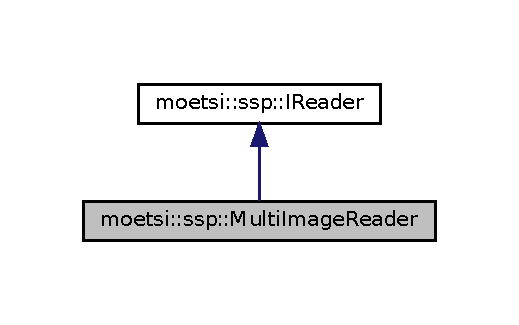
\includegraphics[width=249pt]{classmoetsi_1_1ssp_1_1MultiImageReader__inherit__graph}
\end{center}
\end{figure}


Collaboration diagram for moetsi\+::ssp\+::Multi\+Image\+Reader\+:
\nopagebreak
\begin{figure}[H]
\begin{center}
\leavevmode
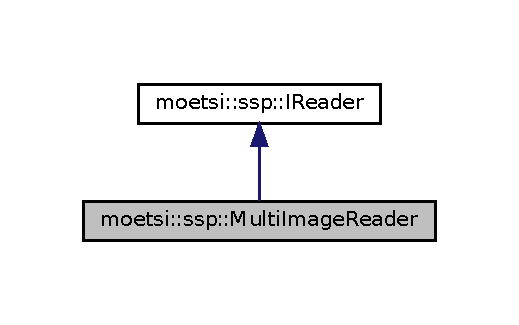
\includegraphics[width=249pt]{classmoetsi_1_1ssp_1_1MultiImageReader__coll__graph}
\end{center}
\end{figure}
\doxysubsection*{Public Member Functions}
\begin{DoxyCompactItemize}
\item 
\mbox{\Hypertarget{classmoetsi_1_1ssp_1_1MultiImageReader_a20a5450c538661d3951ea27a2ff92854}\label{classmoetsi_1_1ssp_1_1MultiImageReader_a20a5450c538661d3951ea27a2ff92854}} 
{\bfseries Multi\+Image\+Reader} (std\+::vector$<$ std\+::string $>$ filename)
\item 
\mbox{\Hypertarget{classmoetsi_1_1ssp_1_1MultiImageReader_a6a0aceb3412f25580876a4fbcedf7ed0}\label{classmoetsi_1_1ssp_1_1MultiImageReader_a6a0aceb3412f25580876a4fbcedf7ed0}} 
virtual std\+::vector$<$ std\+::shared\+\_\+ptr$<$ \mbox{\hyperlink{structmoetsi_1_1ssp_1_1FrameStruct}{Frame\+Struct}} $>$ $>$ \mbox{\hyperlink{classmoetsi_1_1ssp_1_1MultiImageReader_a6a0aceb3412f25580876a4fbcedf7ed0}{Get\+Current\+Frame}} ()
\begin{DoxyCompactList}\small\item\em Get current frame data. \end{DoxyCompactList}\item 
virtual std\+::vector$<$ \mbox{\hyperlink{namespacemoetsi_1_1ssp_a46efdfa2cd5a28ead465dcc8006b5a87}{Frame\+Type}} $>$ \mbox{\hyperlink{classmoetsi_1_1ssp_1_1MultiImageReader_ad5f6cf0cfb1e64bcf569ab0bbfcce9d6}{Get\+Type}} ()
\begin{DoxyCompactList}\small\item\em Get frame types. \end{DoxyCompactList}\item 
virtual bool \mbox{\hyperlink{classmoetsi_1_1ssp_1_1MultiImageReader_a04240c98d28d8949fca4ecdcb04f04f5}{Has\+Next\+Frame}} ()
\begin{DoxyCompactList}\small\item\em Check if there is a next frame. \end{DoxyCompactList}\item 
\mbox{\Hypertarget{classmoetsi_1_1ssp_1_1MultiImageReader_a472e2b97ce7a1c2485abd14c276bb8fe}\label{classmoetsi_1_1ssp_1_1MultiImageReader_a472e2b97ce7a1c2485abd14c276bb8fe}} 
virtual void \mbox{\hyperlink{classmoetsi_1_1ssp_1_1MultiImageReader_a472e2b97ce7a1c2485abd14c276bb8fe}{Next\+Frame}} ()
\begin{DoxyCompactList}\small\item\em Go to next frame. \end{DoxyCompactList}\item 
\mbox{\Hypertarget{classmoetsi_1_1ssp_1_1MultiImageReader_a3a60b57e1db97cb170435dd7f0d4c66d}\label{classmoetsi_1_1ssp_1_1MultiImageReader_a3a60b57e1db97cb170435dd7f0d4c66d}} 
virtual void \mbox{\hyperlink{classmoetsi_1_1ssp_1_1MultiImageReader_a3a60b57e1db97cb170435dd7f0d4c66d}{Reset}} ()
\begin{DoxyCompactList}\small\item\em Reset this reader. \end{DoxyCompactList}\item 
virtual void \mbox{\hyperlink{classmoetsi_1_1ssp_1_1MultiImageReader_a7c552a1ad469660ea0a88b9ca85138ad}{Go\+To\+Frame}} (unsigned int frame\+\_\+id)
\begin{DoxyCompactList}\small\item\em Go to a given frame. \end{DoxyCompactList}\item 
virtual unsigned int \mbox{\hyperlink{classmoetsi_1_1ssp_1_1MultiImageReader_a994eea20e9682c2f4afc9303a34c76f3}{Get\+Current\+Frame\+Id}} ()
\begin{DoxyCompactList}\small\item\em Get current frame number. \end{DoxyCompactList}\item 
virtual unsigned int \mbox{\hyperlink{classmoetsi_1_1ssp_1_1MultiImageReader_ad0a249af66f8e1a063c3e575fc1b94cb}{Get\+Fps}} ()
\begin{DoxyCompactList}\small\item\em Get indicative F\+PS in frame per second. \end{DoxyCompactList}\end{DoxyCompactItemize}


\doxysubsection{Member Function Documentation}
\mbox{\Hypertarget{classmoetsi_1_1ssp_1_1MultiImageReader_a994eea20e9682c2f4afc9303a34c76f3}\label{classmoetsi_1_1ssp_1_1MultiImageReader_a994eea20e9682c2f4afc9303a34c76f3}} 
\index{moetsi::ssp::MultiImageReader@{moetsi::ssp::MultiImageReader}!GetCurrentFrameId@{GetCurrentFrameId}}
\index{GetCurrentFrameId@{GetCurrentFrameId}!moetsi::ssp::MultiImageReader@{moetsi::ssp::MultiImageReader}}
\doxysubsubsection{\texorpdfstring{GetCurrentFrameId()}{GetCurrentFrameId()}}
{\footnotesize\ttfamily unsigned int moetsi\+::ssp\+::\+Multi\+Image\+Reader\+::\+Get\+Current\+Frame\+Id (\begin{DoxyParamCaption}{ }\end{DoxyParamCaption})\hspace{0.3cm}{\ttfamily [virtual]}}



Get current frame number. 

\begin{DoxyReturn}{Returns}
current frame number. 
\end{DoxyReturn}


Implements \mbox{\hyperlink{classmoetsi_1_1ssp_1_1IReader_ac292d83eb06dee277baaa06e281a562d}{moetsi\+::ssp\+::\+I\+Reader}}.

\mbox{\Hypertarget{classmoetsi_1_1ssp_1_1MultiImageReader_ad0a249af66f8e1a063c3e575fc1b94cb}\label{classmoetsi_1_1ssp_1_1MultiImageReader_ad0a249af66f8e1a063c3e575fc1b94cb}} 
\index{moetsi::ssp::MultiImageReader@{moetsi::ssp::MultiImageReader}!GetFps@{GetFps}}
\index{GetFps@{GetFps}!moetsi::ssp::MultiImageReader@{moetsi::ssp::MultiImageReader}}
\doxysubsubsection{\texorpdfstring{GetFps()}{GetFps()}}
{\footnotesize\ttfamily unsigned int moetsi\+::ssp\+::\+Multi\+Image\+Reader\+::\+Get\+Fps (\begin{DoxyParamCaption}{ }\end{DoxyParamCaption})\hspace{0.3cm}{\ttfamily [virtual]}}



Get indicative F\+PS in frame per second. 

\begin{DoxyReturn}{Returns}
the F\+PS number 
\end{DoxyReturn}


Implements \mbox{\hyperlink{classmoetsi_1_1ssp_1_1IReader_a9f6a8650ca290b011b8e5451eeae9f32}{moetsi\+::ssp\+::\+I\+Reader}}.

\mbox{\Hypertarget{classmoetsi_1_1ssp_1_1MultiImageReader_ad5f6cf0cfb1e64bcf569ab0bbfcce9d6}\label{classmoetsi_1_1ssp_1_1MultiImageReader_ad5f6cf0cfb1e64bcf569ab0bbfcce9d6}} 
\index{moetsi::ssp::MultiImageReader@{moetsi::ssp::MultiImageReader}!GetType@{GetType}}
\index{GetType@{GetType}!moetsi::ssp::MultiImageReader@{moetsi::ssp::MultiImageReader}}
\doxysubsubsection{\texorpdfstring{GetType()}{GetType()}}
{\footnotesize\ttfamily std\+::vector$<$ \mbox{\hyperlink{namespacemoetsi_1_1ssp_a46efdfa2cd5a28ead465dcc8006b5a87}{Frame\+Type}} $>$ moetsi\+::ssp\+::\+Multi\+Image\+Reader\+::\+Get\+Type (\begin{DoxyParamCaption}{ }\end{DoxyParamCaption})\hspace{0.3cm}{\ttfamily [virtual]}}



Get frame types. 

\begin{DoxyReturn}{Returns}
a vector of Frame\+Type, listing available data types 
\end{DoxyReturn}


Implements \mbox{\hyperlink{classmoetsi_1_1ssp_1_1IReader_a4116c1931fde7bd66133934ffdca1cce}{moetsi\+::ssp\+::\+I\+Reader}}.

\mbox{\Hypertarget{classmoetsi_1_1ssp_1_1MultiImageReader_a7c552a1ad469660ea0a88b9ca85138ad}\label{classmoetsi_1_1ssp_1_1MultiImageReader_a7c552a1ad469660ea0a88b9ca85138ad}} 
\index{moetsi::ssp::MultiImageReader@{moetsi::ssp::MultiImageReader}!GoToFrame@{GoToFrame}}
\index{GoToFrame@{GoToFrame}!moetsi::ssp::MultiImageReader@{moetsi::ssp::MultiImageReader}}
\doxysubsubsection{\texorpdfstring{GoToFrame()}{GoToFrame()}}
{\footnotesize\ttfamily void moetsi\+::ssp\+::\+Multi\+Image\+Reader\+::\+Go\+To\+Frame (\begin{DoxyParamCaption}\item[{unsigned int}]{frame\+\_\+id }\end{DoxyParamCaption})\hspace{0.3cm}{\ttfamily [virtual]}}



Go to a given frame. 


\begin{DoxyParams}{Parameters}
{\em frame\+\_\+id} & target frame number \\
\hline
\end{DoxyParams}


Implements \mbox{\hyperlink{classmoetsi_1_1ssp_1_1IReader_a6f1be3c06538992cca6d550bd9566681}{moetsi\+::ssp\+::\+I\+Reader}}.

\mbox{\Hypertarget{classmoetsi_1_1ssp_1_1MultiImageReader_a04240c98d28d8949fca4ecdcb04f04f5}\label{classmoetsi_1_1ssp_1_1MultiImageReader_a04240c98d28d8949fca4ecdcb04f04f5}} 
\index{moetsi::ssp::MultiImageReader@{moetsi::ssp::MultiImageReader}!HasNextFrame@{HasNextFrame}}
\index{HasNextFrame@{HasNextFrame}!moetsi::ssp::MultiImageReader@{moetsi::ssp::MultiImageReader}}
\doxysubsubsection{\texorpdfstring{HasNextFrame()}{HasNextFrame()}}
{\footnotesize\ttfamily bool moetsi\+::ssp\+::\+Multi\+Image\+Reader\+::\+Has\+Next\+Frame (\begin{DoxyParamCaption}{ }\end{DoxyParamCaption})\hspace{0.3cm}{\ttfamily [virtual]}}



Check if there is a next frame. 

\begin{DoxyReturn}{Returns}
true if there is a next frame 
\end{DoxyReturn}


Implements \mbox{\hyperlink{classmoetsi_1_1ssp_1_1IReader_af9186ba41e136dc4ec3242b5dd55fa04}{moetsi\+::ssp\+::\+I\+Reader}}.



The documentation for this class was generated from the following files\+:\begin{DoxyCompactItemize}
\item 
\mbox{\hyperlink{multi__image__reader_8h}{multi\+\_\+image\+\_\+reader.\+h}}\item 
\mbox{\hyperlink{multi__image__reader_8cc}{multi\+\_\+image\+\_\+reader.\+cc}}\end{DoxyCompactItemize}

\hypertarget{classmoetsi_1_1ssp_1_1NetworkReader}{}\doxysection{moetsi\+::ssp\+::Network\+Reader Class Reference}
\label{classmoetsi_1_1ssp_1_1NetworkReader}\index{moetsi::ssp::NetworkReader@{moetsi::ssp::NetworkReader}}


Network reader.  




{\ttfamily \#include $<$network\+\_\+reader.\+h$>$}

\doxysubsection*{Public Member Functions}
\begin{DoxyCompactItemize}
\item 
\mbox{\Hypertarget{classmoetsi_1_1ssp_1_1NetworkReader_a9bdd3780ddd272cfcbc906d720e86c83}\label{classmoetsi_1_1ssp_1_1NetworkReader_a9bdd3780ddd272cfcbc906d720e86c83}} 
{\bfseries Network\+Reader} (int port)
\item 
\mbox{\Hypertarget{classmoetsi_1_1ssp_1_1NetworkReader_adfb4188f382d0659d49ff1cecdc5300c}\label{classmoetsi_1_1ssp_1_1NetworkReader_adfb4188f382d0659d49ff1cecdc5300c}} 
void {\bfseries init} ()
\item 
\mbox{\Hypertarget{classmoetsi_1_1ssp_1_1NetworkReader_aa13257b597a09567e0c05b076377df71}\label{classmoetsi_1_1ssp_1_1NetworkReader_aa13257b597a09567e0c05b076377df71}} 
bool {\bfseries Has\+Next\+Frame} ()
\item 
\mbox{\Hypertarget{classmoetsi_1_1ssp_1_1NetworkReader_a874a26e90dc4be7d65e69bdb6f8756c1}\label{classmoetsi_1_1ssp_1_1NetworkReader_a874a26e90dc4be7d65e69bdb6f8756c1}} 
void {\bfseries Next\+Frame} ()
\item 
\mbox{\Hypertarget{classmoetsi_1_1ssp_1_1NetworkReader_aba016077f99da855240a9b181c9ee2d6}\label{classmoetsi_1_1ssp_1_1NetworkReader_aba016077f99da855240a9b181c9ee2d6}} 
std\+::vector$<$ \mbox{\hyperlink{structmoetsi_1_1ssp_1_1FrameStruct}{Frame\+Struct}} $>$ {\bfseries Get\+Current\+Frame} ()
\item 
\mbox{\Hypertarget{classmoetsi_1_1ssp_1_1NetworkReader_a165115474912210dfbf05dc11f0222bd}\label{classmoetsi_1_1ssp_1_1NetworkReader_a165115474912210dfbf05dc11f0222bd}} 
unsigned int {\bfseries Get\+Current\+Frame\+Id} ()
\end{DoxyCompactItemize}


\doxysubsection{Detailed Description}
Network reader. 

The documentation for this class was generated from the following files\+:\begin{DoxyCompactItemize}
\item 
\mbox{\hyperlink{network__reader_8h}{network\+\_\+reader.\+h}}\item 
\mbox{\hyperlink{network__reader_8cc}{network\+\_\+reader.\+cc}}\end{DoxyCompactItemize}

\hypertarget{classmoetsi_1_1ssp_1_1NullEncoder}{}\doxysection{moetsi\+::ssp\+::Null\+Encoder Class Reference}
\label{classmoetsi_1_1ssp_1_1NullEncoder}\index{moetsi::ssp::NullEncoder@{moetsi::ssp::NullEncoder}}


Nullencoder Straight pipe encoder.  




{\ttfamily \#include $<$null\+\_\+encoder.\+h$>$}



Inheritance diagram for moetsi\+::ssp\+::Null\+Encoder\+:
\nopagebreak
\begin{figure}[H]
\begin{center}
\leavevmode
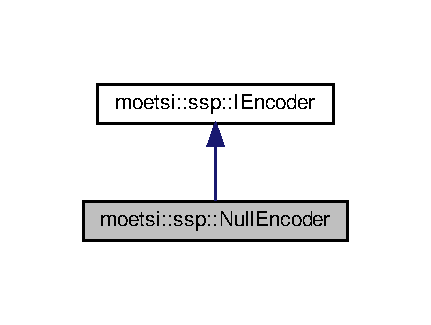
\includegraphics[width=217pt]{classmoetsi_1_1ssp_1_1NullEncoder__inherit__graph}
\end{center}
\end{figure}


Collaboration diagram for moetsi\+::ssp\+::Null\+Encoder\+:
\nopagebreak
\begin{figure}[H]
\begin{center}
\leavevmode
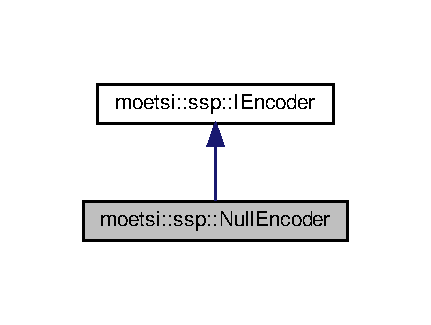
\includegraphics[width=217pt]{classmoetsi_1_1ssp_1_1NullEncoder__coll__graph}
\end{center}
\end{figure}
\doxysubsection*{Public Member Functions}
\begin{DoxyCompactItemize}
\item 
\mbox{\hyperlink{classmoetsi_1_1ssp_1_1NullEncoder_aaae4b8ed8b56ae9526f04853b56d1650}{Null\+Encoder}} (int \+\_\+fps)
\begin{DoxyCompactList}\small\item\em Constructor. \end{DoxyCompactList}\item 
\mbox{\Hypertarget{classmoetsi_1_1ssp_1_1NullEncoder_a503705e0c63e88d583cf587de8d21b78}\label{classmoetsi_1_1ssp_1_1NullEncoder_a503705e0c63e88d583cf587de8d21b78}} 
virtual \mbox{\hyperlink{classmoetsi_1_1ssp_1_1NullEncoder_a503705e0c63e88d583cf587de8d21b78}{$\sim$\+Null\+Encoder}} ()
\begin{DoxyCompactList}\small\item\em Destructor. \end{DoxyCompactList}\item 
virtual void \mbox{\hyperlink{classmoetsi_1_1ssp_1_1NullEncoder_a05f90c640c372d00f45173ec3e9436be}{Add\+Frame\+Struct}} (std\+::shared\+\_\+ptr$<$ \mbox{\hyperlink{structmoetsi_1_1ssp_1_1FrameStruct}{Frame\+Struct}} $>$ \&frame\+\_\+struct)
\begin{DoxyCompactList}\small\item\em Add a frame struct. \end{DoxyCompactList}\item 
\mbox{\Hypertarget{classmoetsi_1_1ssp_1_1NullEncoder_a5fe7215f2b462690208b2a144e962e14}\label{classmoetsi_1_1ssp_1_1NullEncoder_a5fe7215f2b462690208b2a144e962e14}} 
virtual void \mbox{\hyperlink{classmoetsi_1_1ssp_1_1NullEncoder_a5fe7215f2b462690208b2a144e962e14}{Next\+Packet}} ()
\begin{DoxyCompactList}\small\item\em Go to next packet. \end{DoxyCompactList}\item 
virtual bool \mbox{\hyperlink{classmoetsi_1_1ssp_1_1NullEncoder_a359eb668c16a1ef7963214f7f6303af4}{Has\+Next\+Packet}} ()
\begin{DoxyCompactList}\small\item\em Check if there is a next packet. \end{DoxyCompactList}\item 
virtual std\+::shared\+\_\+ptr$<$ \mbox{\hyperlink{structmoetsi_1_1ssp_1_1FrameStruct}{Frame\+Struct}} $>$ \mbox{\hyperlink{classmoetsi_1_1ssp_1_1NullEncoder_ae48926f99c368849ee8822aed10ac1b5}{Current\+Frame\+Encoded}} ()
\begin{DoxyCompactList}\small\item\em Get current encoded frame. \end{DoxyCompactList}\item 
virtual std\+::shared\+\_\+ptr$<$ \mbox{\hyperlink{structmoetsi_1_1ssp_1_1FrameStruct}{Frame\+Struct}} $>$ \mbox{\hyperlink{classmoetsi_1_1ssp_1_1NullEncoder_ad972dfdb93d2f609cdc885c53079ede2}{Current\+Frame\+Original}} ()
\begin{DoxyCompactList}\small\item\em Get current frame in its original format. \end{DoxyCompactList}\item 
virtual std\+::shared\+\_\+ptr$<$ \mbox{\hyperlink{structmoetsi_1_1ssp_1_1CodecParamsStruct}{Codec\+Params\+Struct}} $>$ \mbox{\hyperlink{classmoetsi_1_1ssp_1_1NullEncoder_a29839bd02ad42ecd9cf8e6cce707a9fe}{Get\+Codec\+Params\+Struct}} ()
\begin{DoxyCompactList}\small\item\em Get codec parameters. \end{DoxyCompactList}\item 
virtual unsigned int \mbox{\hyperlink{classmoetsi_1_1ssp_1_1NullEncoder_ad6727fa08528622081aa4eca4aacc6c1}{Get\+Fps}} ()
\begin{DoxyCompactList}\small\item\em Get F\+PS. \end{DoxyCompactList}\end{DoxyCompactItemize}


\doxysubsection{Detailed Description}
Nullencoder Straight pipe encoder. 

\doxysubsection{Constructor \& Destructor Documentation}
\mbox{\Hypertarget{classmoetsi_1_1ssp_1_1NullEncoder_aaae4b8ed8b56ae9526f04853b56d1650}\label{classmoetsi_1_1ssp_1_1NullEncoder_aaae4b8ed8b56ae9526f04853b56d1650}} 
\index{moetsi::ssp::NullEncoder@{moetsi::ssp::NullEncoder}!NullEncoder@{NullEncoder}}
\index{NullEncoder@{NullEncoder}!moetsi::ssp::NullEncoder@{moetsi::ssp::NullEncoder}}
\doxysubsubsection{\texorpdfstring{NullEncoder()}{NullEncoder()}}
{\footnotesize\ttfamily moetsi\+::ssp\+::\+Null\+Encoder\+::\+Null\+Encoder (\begin{DoxyParamCaption}\item[{int}]{\+\_\+fps }\end{DoxyParamCaption})}



Constructor. 


\begin{DoxyParams}{Parameters}
{\em \+\_\+fps} & frame per seconds \\
\hline
\end{DoxyParams}


\doxysubsection{Member Function Documentation}
\mbox{\Hypertarget{classmoetsi_1_1ssp_1_1NullEncoder_a05f90c640c372d00f45173ec3e9436be}\label{classmoetsi_1_1ssp_1_1NullEncoder_a05f90c640c372d00f45173ec3e9436be}} 
\index{moetsi::ssp::NullEncoder@{moetsi::ssp::NullEncoder}!AddFrameStruct@{AddFrameStruct}}
\index{AddFrameStruct@{AddFrameStruct}!moetsi::ssp::NullEncoder@{moetsi::ssp::NullEncoder}}
\doxysubsubsection{\texorpdfstring{AddFrameStruct()}{AddFrameStruct()}}
{\footnotesize\ttfamily void moetsi\+::ssp\+::\+Null\+Encoder\+::\+Add\+Frame\+Struct (\begin{DoxyParamCaption}\item[{std\+::shared\+\_\+ptr$<$ \mbox{\hyperlink{structmoetsi_1_1ssp_1_1FrameStruct}{Frame\+Struct}} $>$ \&}]{frame\+\_\+struct }\end{DoxyParamCaption})\hspace{0.3cm}{\ttfamily [virtual]}}



Add a frame struct. 


\begin{DoxyParams}{Parameters}
{\em frame\+\_\+struct} & \mbox{\hyperlink{structmoetsi_1_1ssp_1_1FrameStruct}{Frame\+Struct}} to add \\
\hline
\end{DoxyParams}


Implements \mbox{\hyperlink{classmoetsi_1_1ssp_1_1IEncoder_a8c223ec82fdd30ee8ee75157306054ec}{moetsi\+::ssp\+::\+I\+Encoder}}.

\mbox{\Hypertarget{classmoetsi_1_1ssp_1_1NullEncoder_ae48926f99c368849ee8822aed10ac1b5}\label{classmoetsi_1_1ssp_1_1NullEncoder_ae48926f99c368849ee8822aed10ac1b5}} 
\index{moetsi::ssp::NullEncoder@{moetsi::ssp::NullEncoder}!CurrentFrameEncoded@{CurrentFrameEncoded}}
\index{CurrentFrameEncoded@{CurrentFrameEncoded}!moetsi::ssp::NullEncoder@{moetsi::ssp::NullEncoder}}
\doxysubsubsection{\texorpdfstring{CurrentFrameEncoded()}{CurrentFrameEncoded()}}
{\footnotesize\ttfamily std\+::shared\+\_\+ptr$<$ \mbox{\hyperlink{structmoetsi_1_1ssp_1_1FrameStruct}{Frame\+Struct}} $>$ moetsi\+::ssp\+::\+Null\+Encoder\+::\+Current\+Frame\+Encoded (\begin{DoxyParamCaption}{ }\end{DoxyParamCaption})\hspace{0.3cm}{\ttfamily [virtual]}}



Get current encoded frame. 

\begin{DoxyReturn}{Returns}
current encoded frame 
\end{DoxyReturn}


Implements \mbox{\hyperlink{classmoetsi_1_1ssp_1_1IEncoder_a178d117518e7c7007414ea9c82bd3ed6}{moetsi\+::ssp\+::\+I\+Encoder}}.

\mbox{\Hypertarget{classmoetsi_1_1ssp_1_1NullEncoder_ad972dfdb93d2f609cdc885c53079ede2}\label{classmoetsi_1_1ssp_1_1NullEncoder_ad972dfdb93d2f609cdc885c53079ede2}} 
\index{moetsi::ssp::NullEncoder@{moetsi::ssp::NullEncoder}!CurrentFrameOriginal@{CurrentFrameOriginal}}
\index{CurrentFrameOriginal@{CurrentFrameOriginal}!moetsi::ssp::NullEncoder@{moetsi::ssp::NullEncoder}}
\doxysubsubsection{\texorpdfstring{CurrentFrameOriginal()}{CurrentFrameOriginal()}}
{\footnotesize\ttfamily std\+::shared\+\_\+ptr$<$ \mbox{\hyperlink{structmoetsi_1_1ssp_1_1FrameStruct}{Frame\+Struct}} $>$ moetsi\+::ssp\+::\+Null\+Encoder\+::\+Current\+Frame\+Original (\begin{DoxyParamCaption}{ }\end{DoxyParamCaption})\hspace{0.3cm}{\ttfamily [virtual]}}



Get current frame in its original format. 

\begin{DoxyReturn}{Returns}
current frame in its original format 
\end{DoxyReturn}


Implements \mbox{\hyperlink{classmoetsi_1_1ssp_1_1IEncoder_ab60bdaae0a85289dfa31a12bab533dc0}{moetsi\+::ssp\+::\+I\+Encoder}}.

\mbox{\Hypertarget{classmoetsi_1_1ssp_1_1NullEncoder_a29839bd02ad42ecd9cf8e6cce707a9fe}\label{classmoetsi_1_1ssp_1_1NullEncoder_a29839bd02ad42ecd9cf8e6cce707a9fe}} 
\index{moetsi::ssp::NullEncoder@{moetsi::ssp::NullEncoder}!GetCodecParamsStruct@{GetCodecParamsStruct}}
\index{GetCodecParamsStruct@{GetCodecParamsStruct}!moetsi::ssp::NullEncoder@{moetsi::ssp::NullEncoder}}
\doxysubsubsection{\texorpdfstring{GetCodecParamsStruct()}{GetCodecParamsStruct()}}
{\footnotesize\ttfamily std\+::shared\+\_\+ptr$<$ \mbox{\hyperlink{structmoetsi_1_1ssp_1_1CodecParamsStruct}{Codec\+Params\+Struct}} $>$ moetsi\+::ssp\+::\+Null\+Encoder\+::\+Get\+Codec\+Params\+Struct (\begin{DoxyParamCaption}{ }\end{DoxyParamCaption})\hspace{0.3cm}{\ttfamily [virtual]}}



Get codec parameters. 

\begin{DoxyReturn}{Returns}
codec parameters 
\end{DoxyReturn}


Implements \mbox{\hyperlink{classmoetsi_1_1ssp_1_1IEncoder_ad5179efaa4c74207766dd64f46f4059a}{moetsi\+::ssp\+::\+I\+Encoder}}.

\mbox{\Hypertarget{classmoetsi_1_1ssp_1_1NullEncoder_ad6727fa08528622081aa4eca4aacc6c1}\label{classmoetsi_1_1ssp_1_1NullEncoder_ad6727fa08528622081aa4eca4aacc6c1}} 
\index{moetsi::ssp::NullEncoder@{moetsi::ssp::NullEncoder}!GetFps@{GetFps}}
\index{GetFps@{GetFps}!moetsi::ssp::NullEncoder@{moetsi::ssp::NullEncoder}}
\doxysubsubsection{\texorpdfstring{GetFps()}{GetFps()}}
{\footnotesize\ttfamily unsigned int moetsi\+::ssp\+::\+Null\+Encoder\+::\+Get\+Fps (\begin{DoxyParamCaption}{ }\end{DoxyParamCaption})\hspace{0.3cm}{\ttfamily [virtual]}}



Get F\+PS. 

\begin{DoxyReturn}{Returns}
F\+PS in frame per second 
\end{DoxyReturn}


Implements \mbox{\hyperlink{classmoetsi_1_1ssp_1_1IEncoder_ae6a865aa52230d81aed1cb5232402f6c}{moetsi\+::ssp\+::\+I\+Encoder}}.

\mbox{\Hypertarget{classmoetsi_1_1ssp_1_1NullEncoder_a359eb668c16a1ef7963214f7f6303af4}\label{classmoetsi_1_1ssp_1_1NullEncoder_a359eb668c16a1ef7963214f7f6303af4}} 
\index{moetsi::ssp::NullEncoder@{moetsi::ssp::NullEncoder}!HasNextPacket@{HasNextPacket}}
\index{HasNextPacket@{HasNextPacket}!moetsi::ssp::NullEncoder@{moetsi::ssp::NullEncoder}}
\doxysubsubsection{\texorpdfstring{HasNextPacket()}{HasNextPacket()}}
{\footnotesize\ttfamily bool moetsi\+::ssp\+::\+Null\+Encoder\+::\+Has\+Next\+Packet (\begin{DoxyParamCaption}{ }\end{DoxyParamCaption})\hspace{0.3cm}{\ttfamily [virtual]}}



Check if there is a next packet. 

\begin{DoxyReturn}{Returns}
true if there is a next packet 
\end{DoxyReturn}


Implements \mbox{\hyperlink{classmoetsi_1_1ssp_1_1IEncoder_a2af8e23d841ef61f6ee4037e56a3694d}{moetsi\+::ssp\+::\+I\+Encoder}}.



The documentation for this class was generated from the following files\+:\begin{DoxyCompactItemize}
\item 
\mbox{\hyperlink{null__encoder_8h}{null\+\_\+encoder.\+h}}\item 
\mbox{\hyperlink{null__encoder_8cc}{null\+\_\+encoder.\+cc}}\end{DoxyCompactItemize}

\hypertarget{classmoetsi_1_1ssp_1_1NvDecoder}{}\doxysection{moetsi\+::ssp\+::Nv\+Decoder Class Reference}
\label{classmoetsi_1_1ssp_1_1NvDecoder}\index{moetsi::ssp::NvDecoder@{moetsi::ssp::NvDecoder}}


Nv\+Pipe decoder.  




{\ttfamily \#include $<$nv\+\_\+decoder.\+h$>$}



Inheritance diagram for moetsi\+::ssp\+::Nv\+Decoder\+:
\nopagebreak
\begin{figure}[H]
\begin{center}
\leavevmode
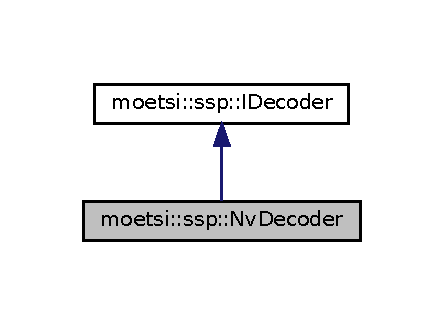
\includegraphics[width=213pt]{classmoetsi_1_1ssp_1_1NvDecoder__inherit__graph}
\end{center}
\end{figure}


Collaboration diagram for moetsi\+::ssp\+::Nv\+Decoder\+:
\nopagebreak
\begin{figure}[H]
\begin{center}
\leavevmode
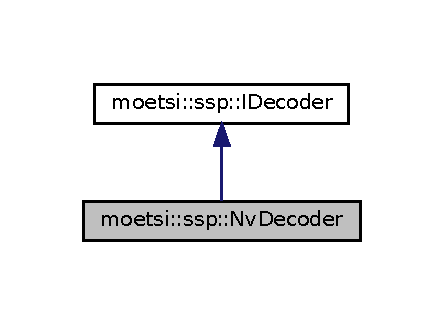
\includegraphics[width=213pt]{classmoetsi_1_1ssp_1_1NvDecoder__coll__graph}
\end{center}
\end{figure}
\doxysubsection*{Public Member Functions}
\begin{DoxyCompactItemize}
\item 
\mbox{\Hypertarget{classmoetsi_1_1ssp_1_1NvDecoder_a40f19812c72e18affbc63a52a3bc223c}\label{classmoetsi_1_1ssp_1_1NvDecoder_a40f19812c72e18affbc63a52a3bc223c}} 
\mbox{\hyperlink{classmoetsi_1_1ssp_1_1NvDecoder_a40f19812c72e18affbc63a52a3bc223c}{Nv\+Decoder}} ()
\begin{DoxyCompactList}\small\item\em Constructor. \end{DoxyCompactList}\item 
\mbox{\Hypertarget{classmoetsi_1_1ssp_1_1NvDecoder_a5371674e976b6dd011448034ceda2ae9}\label{classmoetsi_1_1ssp_1_1NvDecoder_a5371674e976b6dd011448034ceda2ae9}} 
\mbox{\hyperlink{classmoetsi_1_1ssp_1_1NvDecoder_a5371674e976b6dd011448034ceda2ae9}{$\sim$\+Nv\+Decoder}} ()
\begin{DoxyCompactList}\small\item\em Destructor. \end{DoxyCompactList}\item 
void \mbox{\hyperlink{classmoetsi_1_1ssp_1_1NvDecoder_a004e8a1ed5618df951477c9bb955b6ec}{Init}} (std\+::vector$<$ unsigned char $>$ parameter\+\_\+data)
\begin{DoxyCompactList}\small\item\em Initialize. \end{DoxyCompactList}\item 
cv\+::\+Mat \mbox{\hyperlink{classmoetsi_1_1ssp_1_1NvDecoder_a78eb894b6825ac5ec57f5a4f4ecd7e31}{Decode}} (\mbox{\hyperlink{structmoetsi_1_1ssp_1_1FrameStruct}{Frame\+Struct}} \&frame)
\begin{DoxyCompactList}\small\item\em Extract an opencv image from a \mbox{\hyperlink{structmoetsi_1_1ssp_1_1FrameStruct}{Frame\+Struct}}. \end{DoxyCompactList}\end{DoxyCompactItemize}


\doxysubsection{Detailed Description}
Nv\+Pipe decoder. 

\doxysubsection{Member Function Documentation}
\mbox{\Hypertarget{classmoetsi_1_1ssp_1_1NvDecoder_a78eb894b6825ac5ec57f5a4f4ecd7e31}\label{classmoetsi_1_1ssp_1_1NvDecoder_a78eb894b6825ac5ec57f5a4f4ecd7e31}} 
\index{moetsi::ssp::NvDecoder@{moetsi::ssp::NvDecoder}!Decode@{Decode}}
\index{Decode@{Decode}!moetsi::ssp::NvDecoder@{moetsi::ssp::NvDecoder}}
\doxysubsubsection{\texorpdfstring{Decode()}{Decode()}}
{\footnotesize\ttfamily cv\+::\+Mat moetsi\+::ssp\+::\+Nv\+Decoder\+::\+Decode (\begin{DoxyParamCaption}\item[{\mbox{\hyperlink{structmoetsi_1_1ssp_1_1FrameStruct}{Frame\+Struct}} \&}]{frame }\end{DoxyParamCaption})\hspace{0.3cm}{\ttfamily [virtual]}}



Extract an opencv image from a \mbox{\hyperlink{structmoetsi_1_1ssp_1_1FrameStruct}{Frame\+Struct}}. 


\begin{DoxyParams}{Parameters}
{\em data} & \mbox{\hyperlink{structmoetsi_1_1ssp_1_1FrameStruct}{Frame\+Struct}} \\
\hline
\end{DoxyParams}
\begin{DoxyReturn}{Returns}
Open\+CV matrix/image 
\end{DoxyReturn}


Implements \mbox{\hyperlink{classmoetsi_1_1ssp_1_1IDecoder_a1c06604dc4107d3668a4e791c13cc063}{moetsi\+::ssp\+::\+I\+Decoder}}.

\mbox{\Hypertarget{classmoetsi_1_1ssp_1_1NvDecoder_a004e8a1ed5618df951477c9bb955b6ec}\label{classmoetsi_1_1ssp_1_1NvDecoder_a004e8a1ed5618df951477c9bb955b6ec}} 
\index{moetsi::ssp::NvDecoder@{moetsi::ssp::NvDecoder}!Init@{Init}}
\index{Init@{Init}!moetsi::ssp::NvDecoder@{moetsi::ssp::NvDecoder}}
\doxysubsubsection{\texorpdfstring{Init()}{Init()}}
{\footnotesize\ttfamily void moetsi\+::ssp\+::\+Nv\+Decoder\+::\+Init (\begin{DoxyParamCaption}\item[{std\+::vector$<$ unsigned char $>$}]{parameter\+\_\+data }\end{DoxyParamCaption})}



Initialize. 


\begin{DoxyParams}{Parameters}
{\em parameter\+\_\+data} & parameters \\
\hline
\end{DoxyParams}


The documentation for this class was generated from the following files\+:\begin{DoxyCompactItemize}
\item 
\mbox{\hyperlink{nv__decoder_8h}{nv\+\_\+decoder.\+h}}\item 
\mbox{\hyperlink{nv__decoder_8cc}{nv\+\_\+decoder.\+cc}}\end{DoxyCompactItemize}

\hypertarget{classmoetsi_1_1ssp_1_1NvEncoder}{}\doxysection{moetsi\+::ssp\+::Nv\+Encoder Class Reference}
\label{classmoetsi_1_1ssp_1_1NvEncoder}\index{moetsi::ssp::NvEncoder@{moetsi::ssp::NvEncoder}}


Nv\+Pipe encoder.  




{\ttfamily \#include $<$nv\+\_\+encoder.\+h$>$}



Inheritance diagram for moetsi\+::ssp\+::Nv\+Encoder\+:
% FIG 0


Collaboration diagram for moetsi\+::ssp\+::Nv\+Encoder\+:
% FIG 1
\doxysubsection*{Public Member Functions}
\begin{DoxyCompactItemize}
\item 
\mbox{\hyperlink{classmoetsi_1_1ssp_1_1NvEncoder_aab4a3ce1729dba51183b77adcc78aa5e}{Nv\+Encoder}} (Y\+A\+M\+L\+::\+Node \+\_\+codec\+\_\+parameters, unsigned int \+\_\+fps)
\begin{DoxyCompactList}\small\item\em Constructor. \end{DoxyCompactList}\item 
\mbox{\Hypertarget{classmoetsi_1_1ssp_1_1NvEncoder_a1ae3ff63a16da6e5e169684becbb02ed}\label{classmoetsi_1_1ssp_1_1NvEncoder_a1ae3ff63a16da6e5e169684becbb02ed}} 
\mbox{\hyperlink{classmoetsi_1_1ssp_1_1NvEncoder_a1ae3ff63a16da6e5e169684becbb02ed}{$\sim$\+Nv\+Encoder}} ()
\begin{DoxyCompactList}\small\item\em Destructor. \end{DoxyCompactList}\item 
virtual void \mbox{\hyperlink{classmoetsi_1_1ssp_1_1NvEncoder_a99fbcbd5f04c5b3b395167badbf84b2f}{Add\+Frame\+Struct}} (std\+::shared\+\_\+ptr$<$ \mbox{\hyperlink{structmoetsi_1_1ssp_1_1FrameStruct}{Frame\+Struct}} $>$ \&frame\+\_\+struct)=0
\begin{DoxyCompactList}\small\item\em Add a frame struct. \end{DoxyCompactList}\item 
\mbox{\Hypertarget{classmoetsi_1_1ssp_1_1NvEncoder_a1c6d801fbb40e7dea2b33dd2ac154919}\label{classmoetsi_1_1ssp_1_1NvEncoder_a1c6d801fbb40e7dea2b33dd2ac154919}} 
virtual void \mbox{\hyperlink{classmoetsi_1_1ssp_1_1NvEncoder_a1c6d801fbb40e7dea2b33dd2ac154919}{Next\+Packet}} ()
\begin{DoxyCompactList}\small\item\em Go to next packet. \end{DoxyCompactList}\item 
virtual bool \mbox{\hyperlink{classmoetsi_1_1ssp_1_1NvEncoder_a4c0874d9d0d767ae7a33fe9c9a1be1de}{Has\+Next\+Packet}} ()
\begin{DoxyCompactList}\small\item\em Check if there is a next packet. \end{DoxyCompactList}\item 
virtual std\+::shared\+\_\+ptr$<$ \mbox{\hyperlink{structmoetsi_1_1ssp_1_1FrameStruct}{Frame\+Struct}} $>$ \mbox{\hyperlink{classmoetsi_1_1ssp_1_1NvEncoder_adbc7d498e797af8c5bb31b5a2a82efdd}{Current\+Frame\+Encoded}} ()
\begin{DoxyCompactList}\small\item\em Get current encoded frame. \end{DoxyCompactList}\item 
virtual std\+::shared\+\_\+ptr$<$ \mbox{\hyperlink{structmoetsi_1_1ssp_1_1FrameStruct}{Frame\+Struct}} $>$ \mbox{\hyperlink{classmoetsi_1_1ssp_1_1NvEncoder_a56baf331eae448da89ee54b69fec170c}{Current\+Frame\+Original}} ()
\begin{DoxyCompactList}\small\item\em Get current frame in its original format. \end{DoxyCompactList}\item 
virtual std\+::shared\+\_\+ptr$<$ \mbox{\hyperlink{structmoetsi_1_1ssp_1_1CodecParamsStruct}{Codec\+Params\+Struct}} $>$ \mbox{\hyperlink{classmoetsi_1_1ssp_1_1NvEncoder_aa6229a43b12d2f27e27f518fc2229b61}{Get\+Codec\+Params\+Struct}} ()
\begin{DoxyCompactList}\small\item\em Get codec parameters. \end{DoxyCompactList}\item 
virtual unsigned int \mbox{\hyperlink{classmoetsi_1_1ssp_1_1NvEncoder_ab94b826f2aef05afad376132743001d9}{Get\+Fps}} ()
\begin{DoxyCompactList}\small\item\em Get F\+PS. \end{DoxyCompactList}\end{DoxyCompactItemize}


\doxysubsection{Detailed Description}
Nv\+Pipe encoder. 

\doxysubsection{Constructor \& Destructor Documentation}
\mbox{\Hypertarget{classmoetsi_1_1ssp_1_1NvEncoder_aab4a3ce1729dba51183b77adcc78aa5e}\label{classmoetsi_1_1ssp_1_1NvEncoder_aab4a3ce1729dba51183b77adcc78aa5e}} 
\index{moetsi::ssp::NvEncoder@{moetsi::ssp::NvEncoder}!NvEncoder@{NvEncoder}}
\index{NvEncoder@{NvEncoder}!moetsi::ssp::NvEncoder@{moetsi::ssp::NvEncoder}}
\doxysubsubsection{\texorpdfstring{NvEncoder()}{NvEncoder()}}
{\footnotesize\ttfamily moetsi\+::ssp\+::\+Nv\+Encoder\+::\+Nv\+Encoder (\begin{DoxyParamCaption}\item[{Y\+A\+M\+L\+::\+Node}]{\+\_\+codec\+\_\+parameters,  }\item[{unsigned int}]{\+\_\+fps }\end{DoxyParamCaption})}



Constructor. 


\begin{DoxyParams}{Parameters}
{\em \+\_\+codec\+\_\+parameters} & Yaml parameters \\
\hline
{\em \+\_\+fps} & Frame per second \\
\hline
\end{DoxyParams}


\doxysubsection{Member Function Documentation}
\mbox{\Hypertarget{classmoetsi_1_1ssp_1_1NvEncoder_a99fbcbd5f04c5b3b395167badbf84b2f}\label{classmoetsi_1_1ssp_1_1NvEncoder_a99fbcbd5f04c5b3b395167badbf84b2f}} 
\index{moetsi::ssp::NvEncoder@{moetsi::ssp::NvEncoder}!AddFrameStruct@{AddFrameStruct}}
\index{AddFrameStruct@{AddFrameStruct}!moetsi::ssp::NvEncoder@{moetsi::ssp::NvEncoder}}
\doxysubsubsection{\texorpdfstring{AddFrameStruct()}{AddFrameStruct()}}
{\footnotesize\ttfamily void moetsi\+::ssp\+::\+Nv\+Encoder\+::\+Add\+Frame\+Struct (\begin{DoxyParamCaption}\item[{std\+::shared\+\_\+ptr$<$ \mbox{\hyperlink{structmoetsi_1_1ssp_1_1FrameStruct}{Frame\+Struct}} $>$ \&}]{frame\+\_\+struct }\end{DoxyParamCaption})\hspace{0.3cm}{\ttfamily [pure virtual]}}



Add a frame struct. 


\begin{DoxyParams}{Parameters}
{\em frame\+\_\+struct} & \mbox{\hyperlink{structmoetsi_1_1ssp_1_1FrameStruct}{Frame\+Struct}} to add \\
\hline
\end{DoxyParams}


Implements \mbox{\hyperlink{classmoetsi_1_1ssp_1_1IEncoder_a8c223ec82fdd30ee8ee75157306054ec}{moetsi\+::ssp\+::\+I\+Encoder}}.

\mbox{\Hypertarget{classmoetsi_1_1ssp_1_1NvEncoder_adbc7d498e797af8c5bb31b5a2a82efdd}\label{classmoetsi_1_1ssp_1_1NvEncoder_adbc7d498e797af8c5bb31b5a2a82efdd}} 
\index{moetsi::ssp::NvEncoder@{moetsi::ssp::NvEncoder}!CurrentFrameEncoded@{CurrentFrameEncoded}}
\index{CurrentFrameEncoded@{CurrentFrameEncoded}!moetsi::ssp::NvEncoder@{moetsi::ssp::NvEncoder}}
\doxysubsubsection{\texorpdfstring{CurrentFrameEncoded()}{CurrentFrameEncoded()}}
{\footnotesize\ttfamily std\+::shared\+\_\+ptr$<$ \mbox{\hyperlink{structmoetsi_1_1ssp_1_1FrameStruct}{Frame\+Struct}} $>$ moetsi\+::ssp\+::\+Nv\+Encoder\+::\+Current\+Frame\+Encoded (\begin{DoxyParamCaption}{ }\end{DoxyParamCaption})\hspace{0.3cm}{\ttfamily [virtual]}}



Get current encoded frame. 

\begin{DoxyReturn}{Returns}
current encoded frame 
\end{DoxyReturn}


Implements \mbox{\hyperlink{classmoetsi_1_1ssp_1_1IEncoder_a178d117518e7c7007414ea9c82bd3ed6}{moetsi\+::ssp\+::\+I\+Encoder}}.

\mbox{\Hypertarget{classmoetsi_1_1ssp_1_1NvEncoder_a56baf331eae448da89ee54b69fec170c}\label{classmoetsi_1_1ssp_1_1NvEncoder_a56baf331eae448da89ee54b69fec170c}} 
\index{moetsi::ssp::NvEncoder@{moetsi::ssp::NvEncoder}!CurrentFrameOriginal@{CurrentFrameOriginal}}
\index{CurrentFrameOriginal@{CurrentFrameOriginal}!moetsi::ssp::NvEncoder@{moetsi::ssp::NvEncoder}}
\doxysubsubsection{\texorpdfstring{CurrentFrameOriginal()}{CurrentFrameOriginal()}}
{\footnotesize\ttfamily std\+::shared\+\_\+ptr$<$ \mbox{\hyperlink{structmoetsi_1_1ssp_1_1FrameStruct}{Frame\+Struct}} $>$ moetsi\+::ssp\+::\+Nv\+Encoder\+::\+Current\+Frame\+Original (\begin{DoxyParamCaption}{ }\end{DoxyParamCaption})\hspace{0.3cm}{\ttfamily [virtual]}}



Get current frame in its original format. 

\begin{DoxyReturn}{Returns}
current frame in its original format 
\end{DoxyReturn}


Implements \mbox{\hyperlink{classmoetsi_1_1ssp_1_1IEncoder_ab60bdaae0a85289dfa31a12bab533dc0}{moetsi\+::ssp\+::\+I\+Encoder}}.

\mbox{\Hypertarget{classmoetsi_1_1ssp_1_1NvEncoder_aa6229a43b12d2f27e27f518fc2229b61}\label{classmoetsi_1_1ssp_1_1NvEncoder_aa6229a43b12d2f27e27f518fc2229b61}} 
\index{moetsi::ssp::NvEncoder@{moetsi::ssp::NvEncoder}!GetCodecParamsStruct@{GetCodecParamsStruct}}
\index{GetCodecParamsStruct@{GetCodecParamsStruct}!moetsi::ssp::NvEncoder@{moetsi::ssp::NvEncoder}}
\doxysubsubsection{\texorpdfstring{GetCodecParamsStruct()}{GetCodecParamsStruct()}}
{\footnotesize\ttfamily std\+::shared\+\_\+ptr$<$ \mbox{\hyperlink{structmoetsi_1_1ssp_1_1CodecParamsStruct}{Codec\+Params\+Struct}} $>$ moetsi\+::ssp\+::\+Nv\+Encoder\+::\+Get\+Codec\+Params\+Struct (\begin{DoxyParamCaption}{ }\end{DoxyParamCaption})\hspace{0.3cm}{\ttfamily [virtual]}}



Get codec parameters. 

\begin{DoxyReturn}{Returns}
codec parameters 
\end{DoxyReturn}


Implements \mbox{\hyperlink{classmoetsi_1_1ssp_1_1IEncoder_ad5179efaa4c74207766dd64f46f4059a}{moetsi\+::ssp\+::\+I\+Encoder}}.

\mbox{\Hypertarget{classmoetsi_1_1ssp_1_1NvEncoder_ab94b826f2aef05afad376132743001d9}\label{classmoetsi_1_1ssp_1_1NvEncoder_ab94b826f2aef05afad376132743001d9}} 
\index{moetsi::ssp::NvEncoder@{moetsi::ssp::NvEncoder}!GetFps@{GetFps}}
\index{GetFps@{GetFps}!moetsi::ssp::NvEncoder@{moetsi::ssp::NvEncoder}}
\doxysubsubsection{\texorpdfstring{GetFps()}{GetFps()}}
{\footnotesize\ttfamily unsigned int moetsi\+::ssp\+::\+Nv\+Encoder\+::\+Get\+Fps (\begin{DoxyParamCaption}{ }\end{DoxyParamCaption})\hspace{0.3cm}{\ttfamily [virtual]}}



Get F\+PS. 

\begin{DoxyReturn}{Returns}
F\+PS in frame per second 
\end{DoxyReturn}


Implements \mbox{\hyperlink{classmoetsi_1_1ssp_1_1IEncoder_ae6a865aa52230d81aed1cb5232402f6c}{moetsi\+::ssp\+::\+I\+Encoder}}.

\mbox{\Hypertarget{classmoetsi_1_1ssp_1_1NvEncoder_a4c0874d9d0d767ae7a33fe9c9a1be1de}\label{classmoetsi_1_1ssp_1_1NvEncoder_a4c0874d9d0d767ae7a33fe9c9a1be1de}} 
\index{moetsi::ssp::NvEncoder@{moetsi::ssp::NvEncoder}!HasNextPacket@{HasNextPacket}}
\index{HasNextPacket@{HasNextPacket}!moetsi::ssp::NvEncoder@{moetsi::ssp::NvEncoder}}
\doxysubsubsection{\texorpdfstring{HasNextPacket()}{HasNextPacket()}}
{\footnotesize\ttfamily bool moetsi\+::ssp\+::\+Nv\+Encoder\+::\+Has\+Next\+Packet (\begin{DoxyParamCaption}{ }\end{DoxyParamCaption})\hspace{0.3cm}{\ttfamily [virtual]}}



Check if there is a next packet. 

\begin{DoxyReturn}{Returns}
true if there is a next packet 
\end{DoxyReturn}


Implements \mbox{\hyperlink{classmoetsi_1_1ssp_1_1IEncoder_a2af8e23d841ef61f6ee4037e56a3694d}{moetsi\+::ssp\+::\+I\+Encoder}}.



The documentation for this class was generated from the following files\+:\begin{DoxyCompactItemize}
\item 
\mbox{\hyperlink{nv__encoder_8h}{nv\+\_\+encoder.\+h}}\item 
\mbox{\hyperlink{nv__encoder_8cc}{nv\+\_\+encoder.\+cc}}\end{DoxyCompactItemize}

\hypertarget{structmoetsi_1_1ssp_1_1NVPipeDeleter}{}\section{moetsi\+:\+:ssp\+:\+:N\+V\+Pipe\+Deleter Struct Reference}
\label{structmoetsi_1_1ssp_1_1NVPipeDeleter}\index{moetsi\+::ssp\+::\+N\+V\+Pipe\+Deleter@{moetsi\+::ssp\+::\+N\+V\+Pipe\+Deleter}}
\subsection*{Public Member Functions}
\begin{DoxyCompactItemize}
\item 
\mbox{\Hypertarget{structmoetsi_1_1ssp_1_1NVPipeDeleter_a2fe160c6c0b930c2ab76f7c022644b97}\label{structmoetsi_1_1ssp_1_1NVPipeDeleter_a2fe160c6c0b930c2ab76f7c022644b97}} 
void {\bfseries operator()} (Nv\+Pipe $\ast$ptr) const
\end{DoxyCompactItemize}


The documentation for this struct was generated from the following file\+:\begin{DoxyCompactItemize}
\item 
\hyperlink{nvpipe__types_8h}{nvpipe\+\_\+types.\+h}\end{DoxyCompactItemize}

\hypertarget{structmoetsi_1_1ssp_1_1object__human__t}{}\doxysection{moetsi\+::ssp\+::object\+\_\+human\+\_\+t Struct Reference}
\label{structmoetsi_1_1ssp_1_1object__human__t}\index{moetsi::ssp::object\_human\_t@{moetsi::ssp::object\_human\_t}}
\doxysubsection*{Public Member Functions}
\begin{DoxyCompactItemize}
\item 
\mbox{\Hypertarget{structmoetsi_1_1ssp_1_1object__human__t_a632ac93d295ec9eb610b9823667d478d}\label{structmoetsi_1_1ssp_1_1object__human__t_a632ac93d295ec9eb610b9823667d478d}} 
void {\bfseries ntoh} ()
\item 
\mbox{\Hypertarget{structmoetsi_1_1ssp_1_1object__human__t_ae698148d40aa80fb8b977ef324617222}\label{structmoetsi_1_1ssp_1_1object__human__t_ae698148d40aa80fb8b977ef324617222}} 
void {\bfseries hton} ()
\item 
\mbox{\Hypertarget{structmoetsi_1_1ssp_1_1object__human__t_a74cbe99bed62452a496fdd1fd5cc2bdd}\label{structmoetsi_1_1ssp_1_1object__human__t_a74cbe99bed62452a496fdd1fd5cc2bdd}} 
{\footnotesize template$<$class Archive $>$ }\\void {\bfseries serialize} (Archive \&ar)
\item 
\mbox{\Hypertarget{structmoetsi_1_1ssp_1_1object__human__t_a632ac93d295ec9eb610b9823667d478d}\label{structmoetsi_1_1ssp_1_1object__human__t_a632ac93d295ec9eb610b9823667d478d}} 
void {\bfseries ntoh} ()
\item 
\mbox{\Hypertarget{structmoetsi_1_1ssp_1_1object__human__t_ae698148d40aa80fb8b977ef324617222}\label{structmoetsi_1_1ssp_1_1object__human__t_ae698148d40aa80fb8b977ef324617222}} 
void {\bfseries hton} ()
\item 
\mbox{\Hypertarget{structmoetsi_1_1ssp_1_1object__human__t_a74cbe99bed62452a496fdd1fd5cc2bdd}\label{structmoetsi_1_1ssp_1_1object__human__t_a74cbe99bed62452a496fdd1fd5cc2bdd}} 
{\footnotesize template$<$class Archive $>$ }\\void {\bfseries serialize} (Archive \&ar)
\end{DoxyCompactItemize}
\doxysubsection*{Public Attributes}
\begin{DoxyCompactItemize}
\item 
\mbox{\Hypertarget{structmoetsi_1_1ssp_1_1object__human__t_af5a08ca4e16da8d0870be9d8c0d3d0fe}\label{structmoetsi_1_1ssp_1_1object__human__t_af5a08ca4e16da8d0870be9d8c0d3d0fe}} 
int32\+\_\+t {\bfseries Id}
\item 
\mbox{\Hypertarget{structmoetsi_1_1ssp_1_1object__human__t_a073ac7ebeb652d190ac510d818a8b2cb}\label{structmoetsi_1_1ssp_1_1object__human__t_a073ac7ebeb652d190ac510d818a8b2cb}} 
float {\bfseries pelvis\+\_\+x}
\item 
\mbox{\Hypertarget{structmoetsi_1_1ssp_1_1object__human__t_a50d7ce1c94714ec9761935d03e9be028}\label{structmoetsi_1_1ssp_1_1object__human__t_a50d7ce1c94714ec9761935d03e9be028}} 
float {\bfseries pelvis\+\_\+y}
\item 
\mbox{\Hypertarget{structmoetsi_1_1ssp_1_1object__human__t_aac42fab13471b2ac6660c31738c12c0b}\label{structmoetsi_1_1ssp_1_1object__human__t_aac42fab13471b2ac6660c31738c12c0b}} 
float {\bfseries pelvis\+\_\+z}
\item 
\mbox{\Hypertarget{structmoetsi_1_1ssp_1_1object__human__t_a7794248d2c0a23b6baa0671b264953e0}\label{structmoetsi_1_1ssp_1_1object__human__t_a7794248d2c0a23b6baa0671b264953e0}} 
float {\bfseries pelvis\+\_\+\+QX}
\item 
\mbox{\Hypertarget{structmoetsi_1_1ssp_1_1object__human__t_a65ba49d782de587a04db385078559a53}\label{structmoetsi_1_1ssp_1_1object__human__t_a65ba49d782de587a04db385078559a53}} 
float {\bfseries pelvis\+\_\+\+QY}
\item 
\mbox{\Hypertarget{structmoetsi_1_1ssp_1_1object__human__t_a53f10578ae9b469afd3e208035c173d5}\label{structmoetsi_1_1ssp_1_1object__human__t_a53f10578ae9b469afd3e208035c173d5}} 
float {\bfseries pelvis\+\_\+\+QZ}
\item 
\mbox{\Hypertarget{structmoetsi_1_1ssp_1_1object__human__t_ada971104e9cc4ea256ef03cff3085086}\label{structmoetsi_1_1ssp_1_1object__human__t_ada971104e9cc4ea256ef03cff3085086}} 
float {\bfseries pelvis\+\_\+\+QW}
\item 
\mbox{\Hypertarget{structmoetsi_1_1ssp_1_1object__human__t_a3e50681ca83b761560f64a16644ac117}\label{structmoetsi_1_1ssp_1_1object__human__t_a3e50681ca83b761560f64a16644ac117}} 
uint8\+\_\+t {\bfseries pelvis\+\_\+conf}
\item 
\mbox{\Hypertarget{structmoetsi_1_1ssp_1_1object__human__t_aacb8a5b1f0057f9ca95071e81def136b}\label{structmoetsi_1_1ssp_1_1object__human__t_aacb8a5b1f0057f9ca95071e81def136b}} 
float {\bfseries spine\+\_\+navel\+\_\+x}
\item 
\mbox{\Hypertarget{structmoetsi_1_1ssp_1_1object__human__t_a43223c6a563b88fa6502cc2ced38fb95}\label{structmoetsi_1_1ssp_1_1object__human__t_a43223c6a563b88fa6502cc2ced38fb95}} 
float {\bfseries spine\+\_\+navel\+\_\+y}
\item 
\mbox{\Hypertarget{structmoetsi_1_1ssp_1_1object__human__t_a871ee57b6e393c7c61b7e8fa6aba2be5}\label{structmoetsi_1_1ssp_1_1object__human__t_a871ee57b6e393c7c61b7e8fa6aba2be5}} 
float {\bfseries spine\+\_\+navel\+\_\+z}
\item 
\mbox{\Hypertarget{structmoetsi_1_1ssp_1_1object__human__t_ac91c5e79748af202812cde31173745d0}\label{structmoetsi_1_1ssp_1_1object__human__t_ac91c5e79748af202812cde31173745d0}} 
float {\bfseries spine\+\_\+navel\+\_\+\+QX}
\item 
\mbox{\Hypertarget{structmoetsi_1_1ssp_1_1object__human__t_ab4d643d5e5337dbb3ce0848af9b61733}\label{structmoetsi_1_1ssp_1_1object__human__t_ab4d643d5e5337dbb3ce0848af9b61733}} 
float {\bfseries spine\+\_\+navel\+\_\+\+QY}
\item 
\mbox{\Hypertarget{structmoetsi_1_1ssp_1_1object__human__t_aeefe89a319b4e1ee61cdbaaa35246c34}\label{structmoetsi_1_1ssp_1_1object__human__t_aeefe89a319b4e1ee61cdbaaa35246c34}} 
float {\bfseries spine\+\_\+navel\+\_\+\+QZ}
\item 
\mbox{\Hypertarget{structmoetsi_1_1ssp_1_1object__human__t_a8b50ecd21e215ff4b6336e0ddcbaeeef}\label{structmoetsi_1_1ssp_1_1object__human__t_a8b50ecd21e215ff4b6336e0ddcbaeeef}} 
float {\bfseries spine\+\_\+navel\+\_\+\+QW}
\item 
\mbox{\Hypertarget{structmoetsi_1_1ssp_1_1object__human__t_a9055691933320f3909e75da7daf72d72}\label{structmoetsi_1_1ssp_1_1object__human__t_a9055691933320f3909e75da7daf72d72}} 
uint8\+\_\+t {\bfseries spine\+\_\+navel\+\_\+conf}
\item 
\mbox{\Hypertarget{structmoetsi_1_1ssp_1_1object__human__t_a8bbffb8e8b4c2ab8f8b806fd4bf2ab6a}\label{structmoetsi_1_1ssp_1_1object__human__t_a8bbffb8e8b4c2ab8f8b806fd4bf2ab6a}} 
float {\bfseries spine\+\_\+chest\+\_\+x}
\item 
\mbox{\Hypertarget{structmoetsi_1_1ssp_1_1object__human__t_a05960d850dd1c256769d417d4fddd8e3}\label{structmoetsi_1_1ssp_1_1object__human__t_a05960d850dd1c256769d417d4fddd8e3}} 
float {\bfseries spine\+\_\+chest\+\_\+y}
\item 
\mbox{\Hypertarget{structmoetsi_1_1ssp_1_1object__human__t_ab3f682371cc547016464c91ae3c87770}\label{structmoetsi_1_1ssp_1_1object__human__t_ab3f682371cc547016464c91ae3c87770}} 
float {\bfseries spine\+\_\+chest\+\_\+z}
\item 
\mbox{\Hypertarget{structmoetsi_1_1ssp_1_1object__human__t_ab60453b20e25c0698acbb6ec0726b265}\label{structmoetsi_1_1ssp_1_1object__human__t_ab60453b20e25c0698acbb6ec0726b265}} 
float {\bfseries spine\+\_\+chest\+\_\+\+QX}
\item 
\mbox{\Hypertarget{structmoetsi_1_1ssp_1_1object__human__t_ab8156d34cf5d21b3c476468d3ed275dd}\label{structmoetsi_1_1ssp_1_1object__human__t_ab8156d34cf5d21b3c476468d3ed275dd}} 
float {\bfseries spine\+\_\+chest\+\_\+\+QY}
\item 
\mbox{\Hypertarget{structmoetsi_1_1ssp_1_1object__human__t_ab820cc341d87e3f7eb6cba7ca12afb47}\label{structmoetsi_1_1ssp_1_1object__human__t_ab820cc341d87e3f7eb6cba7ca12afb47}} 
float {\bfseries spine\+\_\+chest\+\_\+\+QZ}
\item 
\mbox{\Hypertarget{structmoetsi_1_1ssp_1_1object__human__t_ad15e84d01e74c70027f9100418374563}\label{structmoetsi_1_1ssp_1_1object__human__t_ad15e84d01e74c70027f9100418374563}} 
float {\bfseries spine\+\_\+chest\+\_\+\+QW}
\item 
\mbox{\Hypertarget{structmoetsi_1_1ssp_1_1object__human__t_a08732e04203916ac4f027db34a2b2764}\label{structmoetsi_1_1ssp_1_1object__human__t_a08732e04203916ac4f027db34a2b2764}} 
uint8\+\_\+t {\bfseries spine\+\_\+chest\+\_\+conf}
\item 
\mbox{\Hypertarget{structmoetsi_1_1ssp_1_1object__human__t_a000b559e779faad0a43c6a5b7232b218}\label{structmoetsi_1_1ssp_1_1object__human__t_a000b559e779faad0a43c6a5b7232b218}} 
float {\bfseries neck\+\_\+x}
\item 
\mbox{\Hypertarget{structmoetsi_1_1ssp_1_1object__human__t_a9129f946b3bc39bb550bd5ef8ab33057}\label{structmoetsi_1_1ssp_1_1object__human__t_a9129f946b3bc39bb550bd5ef8ab33057}} 
float {\bfseries neck\+\_\+y}
\item 
\mbox{\Hypertarget{structmoetsi_1_1ssp_1_1object__human__t_a72661a8ded45ce0cffe6a7cbc5cbd5b9}\label{structmoetsi_1_1ssp_1_1object__human__t_a72661a8ded45ce0cffe6a7cbc5cbd5b9}} 
float {\bfseries neck\+\_\+z}
\item 
\mbox{\Hypertarget{structmoetsi_1_1ssp_1_1object__human__t_a2509bd0756bce2e2accda3214a847d76}\label{structmoetsi_1_1ssp_1_1object__human__t_a2509bd0756bce2e2accda3214a847d76}} 
float {\bfseries neck\+\_\+\+QX}
\item 
\mbox{\Hypertarget{structmoetsi_1_1ssp_1_1object__human__t_a34f5be2d71f5faab6c5a6ecb74846038}\label{structmoetsi_1_1ssp_1_1object__human__t_a34f5be2d71f5faab6c5a6ecb74846038}} 
float {\bfseries neck\+\_\+\+QY}
\item 
\mbox{\Hypertarget{structmoetsi_1_1ssp_1_1object__human__t_ab99a5ea10c3fe6b90a962276e0dc70a7}\label{structmoetsi_1_1ssp_1_1object__human__t_ab99a5ea10c3fe6b90a962276e0dc70a7}} 
float {\bfseries neck\+\_\+\+QZ}
\item 
\mbox{\Hypertarget{structmoetsi_1_1ssp_1_1object__human__t_a02ce8d87c0dce4ca0e5127ad2c42bd5c}\label{structmoetsi_1_1ssp_1_1object__human__t_a02ce8d87c0dce4ca0e5127ad2c42bd5c}} 
float {\bfseries neck\+\_\+\+QW}
\item 
\mbox{\Hypertarget{structmoetsi_1_1ssp_1_1object__human__t_ad3bc694f5df7500eb75eb9fa821213d5}\label{structmoetsi_1_1ssp_1_1object__human__t_ad3bc694f5df7500eb75eb9fa821213d5}} 
uint8\+\_\+t {\bfseries neck\+\_\+conf}
\item 
\mbox{\Hypertarget{structmoetsi_1_1ssp_1_1object__human__t_a2930833c55ae71f7d16c6e4cc29d2846}\label{structmoetsi_1_1ssp_1_1object__human__t_a2930833c55ae71f7d16c6e4cc29d2846}} 
float {\bfseries clavicle\+\_\+left\+\_\+x}
\item 
\mbox{\Hypertarget{structmoetsi_1_1ssp_1_1object__human__t_a353c853dc7e6d8f6c3f6703524b34c84}\label{structmoetsi_1_1ssp_1_1object__human__t_a353c853dc7e6d8f6c3f6703524b34c84}} 
float {\bfseries clavicle\+\_\+left\+\_\+y}
\item 
\mbox{\Hypertarget{structmoetsi_1_1ssp_1_1object__human__t_a04312b8f2953f0e016ccec400a9a3c13}\label{structmoetsi_1_1ssp_1_1object__human__t_a04312b8f2953f0e016ccec400a9a3c13}} 
float {\bfseries clavicle\+\_\+left\+\_\+z}
\item 
\mbox{\Hypertarget{structmoetsi_1_1ssp_1_1object__human__t_afd6bb7d509f6e1c16dfe09269ce96ebd}\label{structmoetsi_1_1ssp_1_1object__human__t_afd6bb7d509f6e1c16dfe09269ce96ebd}} 
float {\bfseries clavicle\+\_\+left\+\_\+\+QX}
\item 
\mbox{\Hypertarget{structmoetsi_1_1ssp_1_1object__human__t_abda5452dc013f5dfc4dc0070903a76a5}\label{structmoetsi_1_1ssp_1_1object__human__t_abda5452dc013f5dfc4dc0070903a76a5}} 
float {\bfseries clavicle\+\_\+left\+\_\+\+QY}
\item 
\mbox{\Hypertarget{structmoetsi_1_1ssp_1_1object__human__t_ade4cfc844d9f91f9ca42ac57bce0f058}\label{structmoetsi_1_1ssp_1_1object__human__t_ade4cfc844d9f91f9ca42ac57bce0f058}} 
float {\bfseries clavicle\+\_\+left\+\_\+\+QZ}
\item 
\mbox{\Hypertarget{structmoetsi_1_1ssp_1_1object__human__t_a3caddf6e946e8423b35ac94b04387073}\label{structmoetsi_1_1ssp_1_1object__human__t_a3caddf6e946e8423b35ac94b04387073}} 
float {\bfseries clavicle\+\_\+left\+\_\+\+QW}
\item 
\mbox{\Hypertarget{structmoetsi_1_1ssp_1_1object__human__t_ab00b912f469f77ea66d02ecdb7066d3d}\label{structmoetsi_1_1ssp_1_1object__human__t_ab00b912f469f77ea66d02ecdb7066d3d}} 
uint8\+\_\+t {\bfseries clavicle\+\_\+left\+\_\+conf}
\item 
\mbox{\Hypertarget{structmoetsi_1_1ssp_1_1object__human__t_ac24ad15ede8f6ec125e599d47cffc958}\label{structmoetsi_1_1ssp_1_1object__human__t_ac24ad15ede8f6ec125e599d47cffc958}} 
float {\bfseries shoulder\+\_\+left\+\_\+x}
\item 
\mbox{\Hypertarget{structmoetsi_1_1ssp_1_1object__human__t_a70b35def90d35ae782a68816400d7a30}\label{structmoetsi_1_1ssp_1_1object__human__t_a70b35def90d35ae782a68816400d7a30}} 
float {\bfseries shoulder\+\_\+left\+\_\+y}
\item 
\mbox{\Hypertarget{structmoetsi_1_1ssp_1_1object__human__t_a41a79de66adfb1852796f66c333bbb32}\label{structmoetsi_1_1ssp_1_1object__human__t_a41a79de66adfb1852796f66c333bbb32}} 
float {\bfseries shoulder\+\_\+left\+\_\+z}
\item 
\mbox{\Hypertarget{structmoetsi_1_1ssp_1_1object__human__t_aa878ce1f53be4a9012a152a97e0c81eb}\label{structmoetsi_1_1ssp_1_1object__human__t_aa878ce1f53be4a9012a152a97e0c81eb}} 
float {\bfseries shoulder\+\_\+left\+\_\+\+QX}
\item 
\mbox{\Hypertarget{structmoetsi_1_1ssp_1_1object__human__t_ad14fb5ad66c251777e87bef62c44b55a}\label{structmoetsi_1_1ssp_1_1object__human__t_ad14fb5ad66c251777e87bef62c44b55a}} 
float {\bfseries shoulder\+\_\+left\+\_\+\+QY}
\item 
\mbox{\Hypertarget{structmoetsi_1_1ssp_1_1object__human__t_aa898836d5ef4945745fda27542202a6d}\label{structmoetsi_1_1ssp_1_1object__human__t_aa898836d5ef4945745fda27542202a6d}} 
float {\bfseries shoulder\+\_\+left\+\_\+\+QZ}
\item 
\mbox{\Hypertarget{structmoetsi_1_1ssp_1_1object__human__t_ab4fa5e2e177bf49e54fbcb05336fc5c6}\label{structmoetsi_1_1ssp_1_1object__human__t_ab4fa5e2e177bf49e54fbcb05336fc5c6}} 
float {\bfseries shoulder\+\_\+left\+\_\+\+QW}
\item 
\mbox{\Hypertarget{structmoetsi_1_1ssp_1_1object__human__t_a8e39ae023fb2e22b4685c3e1d9c46568}\label{structmoetsi_1_1ssp_1_1object__human__t_a8e39ae023fb2e22b4685c3e1d9c46568}} 
uint8\+\_\+t {\bfseries shoulder\+\_\+left\+\_\+conf}
\item 
\mbox{\Hypertarget{structmoetsi_1_1ssp_1_1object__human__t_a68118bf97e7239044bec65ac572cf788}\label{structmoetsi_1_1ssp_1_1object__human__t_a68118bf97e7239044bec65ac572cf788}} 
float {\bfseries elbow\+\_\+left\+\_\+x}
\item 
\mbox{\Hypertarget{structmoetsi_1_1ssp_1_1object__human__t_a6da86bd9f2c408b040a21ba844385139}\label{structmoetsi_1_1ssp_1_1object__human__t_a6da86bd9f2c408b040a21ba844385139}} 
float {\bfseries elbow\+\_\+left\+\_\+y}
\item 
\mbox{\Hypertarget{structmoetsi_1_1ssp_1_1object__human__t_a50d22eaefb5edbecdad4ff8f0d9bfb38}\label{structmoetsi_1_1ssp_1_1object__human__t_a50d22eaefb5edbecdad4ff8f0d9bfb38}} 
float {\bfseries elbow\+\_\+left\+\_\+z}
\item 
\mbox{\Hypertarget{structmoetsi_1_1ssp_1_1object__human__t_a65eebb9678ea0bb879edc2667d26b3f0}\label{structmoetsi_1_1ssp_1_1object__human__t_a65eebb9678ea0bb879edc2667d26b3f0}} 
float {\bfseries elbow\+\_\+left\+\_\+\+QX}
\item 
\mbox{\Hypertarget{structmoetsi_1_1ssp_1_1object__human__t_ac4221af811937749a98f24061e96d2f7}\label{structmoetsi_1_1ssp_1_1object__human__t_ac4221af811937749a98f24061e96d2f7}} 
float {\bfseries elbow\+\_\+left\+\_\+\+QY}
\item 
\mbox{\Hypertarget{structmoetsi_1_1ssp_1_1object__human__t_a309b5be23823c3c697cf6c3965f8ed59}\label{structmoetsi_1_1ssp_1_1object__human__t_a309b5be23823c3c697cf6c3965f8ed59}} 
float {\bfseries elbow\+\_\+left\+\_\+\+QZ}
\item 
\mbox{\Hypertarget{structmoetsi_1_1ssp_1_1object__human__t_a48d38baa0b52eceec86f3a9a4630a124}\label{structmoetsi_1_1ssp_1_1object__human__t_a48d38baa0b52eceec86f3a9a4630a124}} 
float {\bfseries elbow\+\_\+left\+\_\+\+QW}
\item 
\mbox{\Hypertarget{structmoetsi_1_1ssp_1_1object__human__t_ac69f4842bffb771f9b0c992b41344cee}\label{structmoetsi_1_1ssp_1_1object__human__t_ac69f4842bffb771f9b0c992b41344cee}} 
uint8\+\_\+t {\bfseries elbow\+\_\+left\+\_\+conf}
\item 
\mbox{\Hypertarget{structmoetsi_1_1ssp_1_1object__human__t_a5416ed0624c54921e7fa6079997eca56}\label{structmoetsi_1_1ssp_1_1object__human__t_a5416ed0624c54921e7fa6079997eca56}} 
float {\bfseries wrist\+\_\+left\+\_\+x}
\item 
\mbox{\Hypertarget{structmoetsi_1_1ssp_1_1object__human__t_a2b9bec9e11c18d56b1b8b4b2c61039dd}\label{structmoetsi_1_1ssp_1_1object__human__t_a2b9bec9e11c18d56b1b8b4b2c61039dd}} 
float {\bfseries wrist\+\_\+left\+\_\+y}
\item 
\mbox{\Hypertarget{structmoetsi_1_1ssp_1_1object__human__t_a00aecf300ac42e66ed158846fdae7bad}\label{structmoetsi_1_1ssp_1_1object__human__t_a00aecf300ac42e66ed158846fdae7bad}} 
float {\bfseries wrist\+\_\+left\+\_\+z}
\item 
\mbox{\Hypertarget{structmoetsi_1_1ssp_1_1object__human__t_a3878e0e5a79ca3e2a8ca92e523e8d591}\label{structmoetsi_1_1ssp_1_1object__human__t_a3878e0e5a79ca3e2a8ca92e523e8d591}} 
float {\bfseries wrist\+\_\+left\+\_\+\+QX}
\item 
\mbox{\Hypertarget{structmoetsi_1_1ssp_1_1object__human__t_a1b5b2aa6272046fe3f12003730ba4ccc}\label{structmoetsi_1_1ssp_1_1object__human__t_a1b5b2aa6272046fe3f12003730ba4ccc}} 
float {\bfseries wrist\+\_\+left\+\_\+\+QY}
\item 
\mbox{\Hypertarget{structmoetsi_1_1ssp_1_1object__human__t_adaa4460e55231ff117a0f39d2706db66}\label{structmoetsi_1_1ssp_1_1object__human__t_adaa4460e55231ff117a0f39d2706db66}} 
float {\bfseries wrist\+\_\+left\+\_\+\+QZ}
\item 
\mbox{\Hypertarget{structmoetsi_1_1ssp_1_1object__human__t_a5a3fbcc3f1698dcaa73041b833f0c8c1}\label{structmoetsi_1_1ssp_1_1object__human__t_a5a3fbcc3f1698dcaa73041b833f0c8c1}} 
float {\bfseries wrist\+\_\+left\+\_\+\+QW}
\item 
\mbox{\Hypertarget{structmoetsi_1_1ssp_1_1object__human__t_a9873865e778a2285ec360dd3edee15af}\label{structmoetsi_1_1ssp_1_1object__human__t_a9873865e778a2285ec360dd3edee15af}} 
uint8\+\_\+t {\bfseries wrist\+\_\+left\+\_\+conf}
\item 
\mbox{\Hypertarget{structmoetsi_1_1ssp_1_1object__human__t_a497b6ffd554803231b30f8b0eda8a278}\label{structmoetsi_1_1ssp_1_1object__human__t_a497b6ffd554803231b30f8b0eda8a278}} 
float {\bfseries hand\+\_\+left\+\_\+x}
\item 
\mbox{\Hypertarget{structmoetsi_1_1ssp_1_1object__human__t_a28dca112d8b55b51b5a7d1355e1e918e}\label{structmoetsi_1_1ssp_1_1object__human__t_a28dca112d8b55b51b5a7d1355e1e918e}} 
float {\bfseries hand\+\_\+left\+\_\+y}
\item 
\mbox{\Hypertarget{structmoetsi_1_1ssp_1_1object__human__t_aadb7add6249cf7490ed19c7e25aa462f}\label{structmoetsi_1_1ssp_1_1object__human__t_aadb7add6249cf7490ed19c7e25aa462f}} 
float {\bfseries hand\+\_\+left\+\_\+z}
\item 
\mbox{\Hypertarget{structmoetsi_1_1ssp_1_1object__human__t_a7a9136627c32e7b8d33d1c8a91479b14}\label{structmoetsi_1_1ssp_1_1object__human__t_a7a9136627c32e7b8d33d1c8a91479b14}} 
float {\bfseries hand\+\_\+left\+\_\+\+QX}
\item 
\mbox{\Hypertarget{structmoetsi_1_1ssp_1_1object__human__t_aad3691026eb24457475982de94d4eca9}\label{structmoetsi_1_1ssp_1_1object__human__t_aad3691026eb24457475982de94d4eca9}} 
float {\bfseries hand\+\_\+left\+\_\+\+QY}
\item 
\mbox{\Hypertarget{structmoetsi_1_1ssp_1_1object__human__t_a343e8b6ce08c76f2f16d66d249d4a62e}\label{structmoetsi_1_1ssp_1_1object__human__t_a343e8b6ce08c76f2f16d66d249d4a62e}} 
float {\bfseries hand\+\_\+left\+\_\+\+QZ}
\item 
\mbox{\Hypertarget{structmoetsi_1_1ssp_1_1object__human__t_a69c4a08d5220f26b40018b3fcffa40d9}\label{structmoetsi_1_1ssp_1_1object__human__t_a69c4a08d5220f26b40018b3fcffa40d9}} 
float {\bfseries hand\+\_\+left\+\_\+\+QW}
\item 
\mbox{\Hypertarget{structmoetsi_1_1ssp_1_1object__human__t_a61c23e40de2e727753320477e97a8ff4}\label{structmoetsi_1_1ssp_1_1object__human__t_a61c23e40de2e727753320477e97a8ff4}} 
uint8\+\_\+t {\bfseries hand\+\_\+left\+\_\+conf}
\item 
\mbox{\Hypertarget{structmoetsi_1_1ssp_1_1object__human__t_a5a7d9599f3e5f08948a6037afbd2de0b}\label{structmoetsi_1_1ssp_1_1object__human__t_a5a7d9599f3e5f08948a6037afbd2de0b}} 
float {\bfseries handtip\+\_\+left\+\_\+x}
\item 
\mbox{\Hypertarget{structmoetsi_1_1ssp_1_1object__human__t_a9775632ee6f3cd4efc00ebf7bfef3f69}\label{structmoetsi_1_1ssp_1_1object__human__t_a9775632ee6f3cd4efc00ebf7bfef3f69}} 
float {\bfseries handtip\+\_\+left\+\_\+y}
\item 
\mbox{\Hypertarget{structmoetsi_1_1ssp_1_1object__human__t_a11f7930ebc0a78bcc35939039c67bfe5}\label{structmoetsi_1_1ssp_1_1object__human__t_a11f7930ebc0a78bcc35939039c67bfe5}} 
float {\bfseries handtip\+\_\+left\+\_\+z}
\item 
\mbox{\Hypertarget{structmoetsi_1_1ssp_1_1object__human__t_a41d1f3852f38c8d71155d2ac61ec6050}\label{structmoetsi_1_1ssp_1_1object__human__t_a41d1f3852f38c8d71155d2ac61ec6050}} 
float {\bfseries handtip\+\_\+left\+\_\+\+QX}
\item 
\mbox{\Hypertarget{structmoetsi_1_1ssp_1_1object__human__t_af1ca39b5fd2a052e67537f6f3136bf76}\label{structmoetsi_1_1ssp_1_1object__human__t_af1ca39b5fd2a052e67537f6f3136bf76}} 
float {\bfseries handtip\+\_\+left\+\_\+\+QY}
\item 
\mbox{\Hypertarget{structmoetsi_1_1ssp_1_1object__human__t_abc5ba2882a168566f5819046c9e09f84}\label{structmoetsi_1_1ssp_1_1object__human__t_abc5ba2882a168566f5819046c9e09f84}} 
float {\bfseries handtip\+\_\+left\+\_\+\+QZ}
\item 
\mbox{\Hypertarget{structmoetsi_1_1ssp_1_1object__human__t_a4f9dff0be27b194022942d9a5431824d}\label{structmoetsi_1_1ssp_1_1object__human__t_a4f9dff0be27b194022942d9a5431824d}} 
float {\bfseries handtip\+\_\+left\+\_\+\+QW}
\item 
\mbox{\Hypertarget{structmoetsi_1_1ssp_1_1object__human__t_a526f12344d981f8b603d83a1c33a088f}\label{structmoetsi_1_1ssp_1_1object__human__t_a526f12344d981f8b603d83a1c33a088f}} 
uint8\+\_\+t {\bfseries handtip\+\_\+left\+\_\+conf}
\item 
\mbox{\Hypertarget{structmoetsi_1_1ssp_1_1object__human__t_a39bea1f2777a14d30e9abd5ae0ae3145}\label{structmoetsi_1_1ssp_1_1object__human__t_a39bea1f2777a14d30e9abd5ae0ae3145}} 
float {\bfseries thumb\+\_\+left\+\_\+x}
\item 
\mbox{\Hypertarget{structmoetsi_1_1ssp_1_1object__human__t_a4ba855f4746d354b225fb59d3ad839d6}\label{structmoetsi_1_1ssp_1_1object__human__t_a4ba855f4746d354b225fb59d3ad839d6}} 
float {\bfseries thumb\+\_\+left\+\_\+y}
\item 
\mbox{\Hypertarget{structmoetsi_1_1ssp_1_1object__human__t_a02c0a8909a9c8515584e12b93bc4864a}\label{structmoetsi_1_1ssp_1_1object__human__t_a02c0a8909a9c8515584e12b93bc4864a}} 
float {\bfseries thumb\+\_\+left\+\_\+z}
\item 
\mbox{\Hypertarget{structmoetsi_1_1ssp_1_1object__human__t_a8cbd0d536d59f5c2f57c4f14d9580759}\label{structmoetsi_1_1ssp_1_1object__human__t_a8cbd0d536d59f5c2f57c4f14d9580759}} 
float {\bfseries thumb\+\_\+left\+\_\+\+QX}
\item 
\mbox{\Hypertarget{structmoetsi_1_1ssp_1_1object__human__t_a3bae07cd70d4d972462c090f3fe50947}\label{structmoetsi_1_1ssp_1_1object__human__t_a3bae07cd70d4d972462c090f3fe50947}} 
float {\bfseries thumb\+\_\+left\+\_\+\+QY}
\item 
\mbox{\Hypertarget{structmoetsi_1_1ssp_1_1object__human__t_ac9b3c83a1f9b02031666555e22a1ed52}\label{structmoetsi_1_1ssp_1_1object__human__t_ac9b3c83a1f9b02031666555e22a1ed52}} 
float {\bfseries thumb\+\_\+left\+\_\+\+QZ}
\item 
\mbox{\Hypertarget{structmoetsi_1_1ssp_1_1object__human__t_a4d814ca60bf38756e1c93a15a243018d}\label{structmoetsi_1_1ssp_1_1object__human__t_a4d814ca60bf38756e1c93a15a243018d}} 
float {\bfseries thumb\+\_\+left\+\_\+\+QW}
\item 
\mbox{\Hypertarget{structmoetsi_1_1ssp_1_1object__human__t_a58836bcb9c901de0840fc4607eb57251}\label{structmoetsi_1_1ssp_1_1object__human__t_a58836bcb9c901de0840fc4607eb57251}} 
uint8\+\_\+t {\bfseries thumb\+\_\+left\+\_\+conf}
\item 
\mbox{\Hypertarget{structmoetsi_1_1ssp_1_1object__human__t_a2094cc7d81aafa061fc5aaa3e210784a}\label{structmoetsi_1_1ssp_1_1object__human__t_a2094cc7d81aafa061fc5aaa3e210784a}} 
float {\bfseries clavicle\+\_\+right\+\_\+x}
\item 
\mbox{\Hypertarget{structmoetsi_1_1ssp_1_1object__human__t_a63ba74455cfd7944732831259bae31d4}\label{structmoetsi_1_1ssp_1_1object__human__t_a63ba74455cfd7944732831259bae31d4}} 
float {\bfseries clavicle\+\_\+right\+\_\+y}
\item 
\mbox{\Hypertarget{structmoetsi_1_1ssp_1_1object__human__t_a47defdd82f7def6cbfbe9da1402de693}\label{structmoetsi_1_1ssp_1_1object__human__t_a47defdd82f7def6cbfbe9da1402de693}} 
float {\bfseries clavicle\+\_\+right\+\_\+z}
\item 
\mbox{\Hypertarget{structmoetsi_1_1ssp_1_1object__human__t_aa502cabc62e8d8d0bd921a139848e4bc}\label{structmoetsi_1_1ssp_1_1object__human__t_aa502cabc62e8d8d0bd921a139848e4bc}} 
float {\bfseries clavicle\+\_\+right\+\_\+\+QX}
\item 
\mbox{\Hypertarget{structmoetsi_1_1ssp_1_1object__human__t_a87a9002378fb8c5a64712cf4f04f0fb5}\label{structmoetsi_1_1ssp_1_1object__human__t_a87a9002378fb8c5a64712cf4f04f0fb5}} 
float {\bfseries clavicle\+\_\+right\+\_\+\+QY}
\item 
\mbox{\Hypertarget{structmoetsi_1_1ssp_1_1object__human__t_ae5ef88dd46b1b9f08182e6a0584a79ba}\label{structmoetsi_1_1ssp_1_1object__human__t_ae5ef88dd46b1b9f08182e6a0584a79ba}} 
float {\bfseries clavicle\+\_\+right\+\_\+\+QZ}
\item 
\mbox{\Hypertarget{structmoetsi_1_1ssp_1_1object__human__t_a1a31a03a1456d081222d0f2e1dd7e51c}\label{structmoetsi_1_1ssp_1_1object__human__t_a1a31a03a1456d081222d0f2e1dd7e51c}} 
float {\bfseries clavicle\+\_\+right\+\_\+\+QW}
\item 
\mbox{\Hypertarget{structmoetsi_1_1ssp_1_1object__human__t_a265c52f49ea026952052bf360bd3a004}\label{structmoetsi_1_1ssp_1_1object__human__t_a265c52f49ea026952052bf360bd3a004}} 
uint8\+\_\+t {\bfseries clavicle\+\_\+right\+\_\+conf}
\item 
\mbox{\Hypertarget{structmoetsi_1_1ssp_1_1object__human__t_a73aa3673ecc94e20dd593c81141a090d}\label{structmoetsi_1_1ssp_1_1object__human__t_a73aa3673ecc94e20dd593c81141a090d}} 
float {\bfseries shoulder\+\_\+right\+\_\+x}
\item 
\mbox{\Hypertarget{structmoetsi_1_1ssp_1_1object__human__t_af257ad21f741264ed9aff6be2043509c}\label{structmoetsi_1_1ssp_1_1object__human__t_af257ad21f741264ed9aff6be2043509c}} 
float {\bfseries shoulder\+\_\+right\+\_\+y}
\item 
\mbox{\Hypertarget{structmoetsi_1_1ssp_1_1object__human__t_a601dde2136cdd831f6b1e90a310f8054}\label{structmoetsi_1_1ssp_1_1object__human__t_a601dde2136cdd831f6b1e90a310f8054}} 
float {\bfseries shoulder\+\_\+right\+\_\+z}
\item 
\mbox{\Hypertarget{structmoetsi_1_1ssp_1_1object__human__t_a2194e2ed013baa9263fa5777116c4086}\label{structmoetsi_1_1ssp_1_1object__human__t_a2194e2ed013baa9263fa5777116c4086}} 
float {\bfseries shoulder\+\_\+right\+\_\+\+QX}
\item 
\mbox{\Hypertarget{structmoetsi_1_1ssp_1_1object__human__t_a02335ad8e55de2ce830eb503de0e4ea6}\label{structmoetsi_1_1ssp_1_1object__human__t_a02335ad8e55de2ce830eb503de0e4ea6}} 
float {\bfseries shoulder\+\_\+right\+\_\+\+QY}
\item 
\mbox{\Hypertarget{structmoetsi_1_1ssp_1_1object__human__t_a1a29e7096ad74625efec8d9255b283b7}\label{structmoetsi_1_1ssp_1_1object__human__t_a1a29e7096ad74625efec8d9255b283b7}} 
float {\bfseries shoulder\+\_\+right\+\_\+\+QZ}
\item 
\mbox{\Hypertarget{structmoetsi_1_1ssp_1_1object__human__t_a8e38ab666e7fde19502bc229fbf30e0a}\label{structmoetsi_1_1ssp_1_1object__human__t_a8e38ab666e7fde19502bc229fbf30e0a}} 
float {\bfseries shoulder\+\_\+right\+\_\+\+QW}
\item 
\mbox{\Hypertarget{structmoetsi_1_1ssp_1_1object__human__t_ae9335674a70e485b106c5fea5d69098f}\label{structmoetsi_1_1ssp_1_1object__human__t_ae9335674a70e485b106c5fea5d69098f}} 
uint8\+\_\+t {\bfseries shoulder\+\_\+right\+\_\+conf}
\item 
\mbox{\Hypertarget{structmoetsi_1_1ssp_1_1object__human__t_a96e1f0c853d98f1d2d355bbd0f58727a}\label{structmoetsi_1_1ssp_1_1object__human__t_a96e1f0c853d98f1d2d355bbd0f58727a}} 
float {\bfseries elbow\+\_\+right\+\_\+x}
\item 
\mbox{\Hypertarget{structmoetsi_1_1ssp_1_1object__human__t_af21db0c8692365dac9797e0f7b421d0f}\label{structmoetsi_1_1ssp_1_1object__human__t_af21db0c8692365dac9797e0f7b421d0f}} 
float {\bfseries elbow\+\_\+right\+\_\+y}
\item 
\mbox{\Hypertarget{structmoetsi_1_1ssp_1_1object__human__t_a6caf66a2dddaf948257ee2fc08aa23b4}\label{structmoetsi_1_1ssp_1_1object__human__t_a6caf66a2dddaf948257ee2fc08aa23b4}} 
float {\bfseries elbow\+\_\+right\+\_\+z}
\item 
\mbox{\Hypertarget{structmoetsi_1_1ssp_1_1object__human__t_adc8946a855286db2b6b69233038e7d8d}\label{structmoetsi_1_1ssp_1_1object__human__t_adc8946a855286db2b6b69233038e7d8d}} 
float {\bfseries elbow\+\_\+right\+\_\+\+QX}
\item 
\mbox{\Hypertarget{structmoetsi_1_1ssp_1_1object__human__t_a41a218b7fb1ce0199567b6bb7f85a593}\label{structmoetsi_1_1ssp_1_1object__human__t_a41a218b7fb1ce0199567b6bb7f85a593}} 
float {\bfseries elbow\+\_\+right\+\_\+\+QY}
\item 
\mbox{\Hypertarget{structmoetsi_1_1ssp_1_1object__human__t_a53aab1ab994a6bd7085f8bc94a1cb68d}\label{structmoetsi_1_1ssp_1_1object__human__t_a53aab1ab994a6bd7085f8bc94a1cb68d}} 
float {\bfseries elbow\+\_\+right\+\_\+\+QZ}
\item 
\mbox{\Hypertarget{structmoetsi_1_1ssp_1_1object__human__t_a1852d462ba3f2f766f7e99c4e7790efd}\label{structmoetsi_1_1ssp_1_1object__human__t_a1852d462ba3f2f766f7e99c4e7790efd}} 
float {\bfseries elbow\+\_\+right\+\_\+\+QW}
\item 
\mbox{\Hypertarget{structmoetsi_1_1ssp_1_1object__human__t_adbf5fc68484eb8dba8c7d190da3bd41c}\label{structmoetsi_1_1ssp_1_1object__human__t_adbf5fc68484eb8dba8c7d190da3bd41c}} 
uint8\+\_\+t {\bfseries elbow\+\_\+right\+\_\+conf}
\item 
\mbox{\Hypertarget{structmoetsi_1_1ssp_1_1object__human__t_a6dfe0e7ed4f6f0b822189206a79462e5}\label{structmoetsi_1_1ssp_1_1object__human__t_a6dfe0e7ed4f6f0b822189206a79462e5}} 
float {\bfseries wrist\+\_\+right\+\_\+x}
\item 
\mbox{\Hypertarget{structmoetsi_1_1ssp_1_1object__human__t_ae6abb85944973e36b8768221581ebaaa}\label{structmoetsi_1_1ssp_1_1object__human__t_ae6abb85944973e36b8768221581ebaaa}} 
float {\bfseries wrist\+\_\+right\+\_\+y}
\item 
\mbox{\Hypertarget{structmoetsi_1_1ssp_1_1object__human__t_ae01b00a5eed7660440f5d1e79f54b372}\label{structmoetsi_1_1ssp_1_1object__human__t_ae01b00a5eed7660440f5d1e79f54b372}} 
float {\bfseries wrist\+\_\+right\+\_\+z}
\item 
\mbox{\Hypertarget{structmoetsi_1_1ssp_1_1object__human__t_aea8abc32b2bc719afd5d9f2864da5501}\label{structmoetsi_1_1ssp_1_1object__human__t_aea8abc32b2bc719afd5d9f2864da5501}} 
float {\bfseries wrist\+\_\+right\+\_\+\+QX}
\item 
\mbox{\Hypertarget{structmoetsi_1_1ssp_1_1object__human__t_a8f64592c7b84e3c679be1937d01d3ddd}\label{structmoetsi_1_1ssp_1_1object__human__t_a8f64592c7b84e3c679be1937d01d3ddd}} 
float {\bfseries wrist\+\_\+right\+\_\+\+QY}
\item 
\mbox{\Hypertarget{structmoetsi_1_1ssp_1_1object__human__t_a8643aab0689450c26beef1e1e6af4287}\label{structmoetsi_1_1ssp_1_1object__human__t_a8643aab0689450c26beef1e1e6af4287}} 
float {\bfseries wrist\+\_\+right\+\_\+\+QZ}
\item 
\mbox{\Hypertarget{structmoetsi_1_1ssp_1_1object__human__t_afe21f7da0d260533c92cdf682a164c24}\label{structmoetsi_1_1ssp_1_1object__human__t_afe21f7da0d260533c92cdf682a164c24}} 
float {\bfseries wrist\+\_\+right\+\_\+\+QW}
\item 
\mbox{\Hypertarget{structmoetsi_1_1ssp_1_1object__human__t_a9439ab4d4b020a6b128f14fe145a0a76}\label{structmoetsi_1_1ssp_1_1object__human__t_a9439ab4d4b020a6b128f14fe145a0a76}} 
uint8\+\_\+t {\bfseries wrist\+\_\+right\+\_\+conf}
\item 
\mbox{\Hypertarget{structmoetsi_1_1ssp_1_1object__human__t_af536c2f49aedf2182c0caa0c61530c1c}\label{structmoetsi_1_1ssp_1_1object__human__t_af536c2f49aedf2182c0caa0c61530c1c}} 
float {\bfseries hand\+\_\+right\+\_\+x}
\item 
\mbox{\Hypertarget{structmoetsi_1_1ssp_1_1object__human__t_ae0fb5e4af56f4ae12eed671bd9a70e72}\label{structmoetsi_1_1ssp_1_1object__human__t_ae0fb5e4af56f4ae12eed671bd9a70e72}} 
float {\bfseries hand\+\_\+right\+\_\+y}
\item 
\mbox{\Hypertarget{structmoetsi_1_1ssp_1_1object__human__t_ae898591cc6d11cb419b3af26c36bfd7a}\label{structmoetsi_1_1ssp_1_1object__human__t_ae898591cc6d11cb419b3af26c36bfd7a}} 
float {\bfseries hand\+\_\+right\+\_\+z}
\item 
\mbox{\Hypertarget{structmoetsi_1_1ssp_1_1object__human__t_a99c803aa32ccc3142d50222813b696ca}\label{structmoetsi_1_1ssp_1_1object__human__t_a99c803aa32ccc3142d50222813b696ca}} 
float {\bfseries hand\+\_\+right\+\_\+\+QX}
\item 
\mbox{\Hypertarget{structmoetsi_1_1ssp_1_1object__human__t_a1405054f6796f5fdff6630902f12b91e}\label{structmoetsi_1_1ssp_1_1object__human__t_a1405054f6796f5fdff6630902f12b91e}} 
float {\bfseries hand\+\_\+right\+\_\+\+QY}
\item 
\mbox{\Hypertarget{structmoetsi_1_1ssp_1_1object__human__t_aea8e4a79a726e434d2c81849715bcab4}\label{structmoetsi_1_1ssp_1_1object__human__t_aea8e4a79a726e434d2c81849715bcab4}} 
float {\bfseries hand\+\_\+right\+\_\+\+QZ}
\item 
\mbox{\Hypertarget{structmoetsi_1_1ssp_1_1object__human__t_a89edb5ec108ff0848137c748e862c99e}\label{structmoetsi_1_1ssp_1_1object__human__t_a89edb5ec108ff0848137c748e862c99e}} 
float {\bfseries hand\+\_\+right\+\_\+\+QW}
\item 
\mbox{\Hypertarget{structmoetsi_1_1ssp_1_1object__human__t_aad69f0da762de9d26238bd1b8d9eab6b}\label{structmoetsi_1_1ssp_1_1object__human__t_aad69f0da762de9d26238bd1b8d9eab6b}} 
uint8\+\_\+t {\bfseries hand\+\_\+right\+\_\+conf}
\item 
\mbox{\Hypertarget{structmoetsi_1_1ssp_1_1object__human__t_ad5b1fe6a26b5c51681c88e3203817caf}\label{structmoetsi_1_1ssp_1_1object__human__t_ad5b1fe6a26b5c51681c88e3203817caf}} 
float {\bfseries handtip\+\_\+right\+\_\+x}
\item 
\mbox{\Hypertarget{structmoetsi_1_1ssp_1_1object__human__t_af3b566862c805cd385dc14a4743675ac}\label{structmoetsi_1_1ssp_1_1object__human__t_af3b566862c805cd385dc14a4743675ac}} 
float {\bfseries handtip\+\_\+right\+\_\+y}
\item 
\mbox{\Hypertarget{structmoetsi_1_1ssp_1_1object__human__t_a9d4d7ab68bd622d37573d4da4156126f}\label{structmoetsi_1_1ssp_1_1object__human__t_a9d4d7ab68bd622d37573d4da4156126f}} 
float {\bfseries handtip\+\_\+right\+\_\+z}
\item 
\mbox{\Hypertarget{structmoetsi_1_1ssp_1_1object__human__t_ac4fc308fb2978eac28ba3f471b8aaf71}\label{structmoetsi_1_1ssp_1_1object__human__t_ac4fc308fb2978eac28ba3f471b8aaf71}} 
float {\bfseries handtip\+\_\+right\+\_\+\+QX}
\item 
\mbox{\Hypertarget{structmoetsi_1_1ssp_1_1object__human__t_aef8575d1e74fdf2d06fa0c2397950b6b}\label{structmoetsi_1_1ssp_1_1object__human__t_aef8575d1e74fdf2d06fa0c2397950b6b}} 
float {\bfseries handtip\+\_\+right\+\_\+\+QY}
\item 
\mbox{\Hypertarget{structmoetsi_1_1ssp_1_1object__human__t_a1517ff830b9a684ab5ed92695dfe1169}\label{structmoetsi_1_1ssp_1_1object__human__t_a1517ff830b9a684ab5ed92695dfe1169}} 
float {\bfseries handtip\+\_\+right\+\_\+\+QZ}
\item 
\mbox{\Hypertarget{structmoetsi_1_1ssp_1_1object__human__t_a51ae1ab0bbae8dd91c080b4181650daf}\label{structmoetsi_1_1ssp_1_1object__human__t_a51ae1ab0bbae8dd91c080b4181650daf}} 
float {\bfseries handtip\+\_\+right\+\_\+\+QW}
\item 
\mbox{\Hypertarget{structmoetsi_1_1ssp_1_1object__human__t_a0a134d7980f018e2d7b940d3bd214f43}\label{structmoetsi_1_1ssp_1_1object__human__t_a0a134d7980f018e2d7b940d3bd214f43}} 
uint8\+\_\+t {\bfseries handtip\+\_\+right\+\_\+conf}
\item 
\mbox{\Hypertarget{structmoetsi_1_1ssp_1_1object__human__t_a21c3aabafff91f3356a5bb5d1365a5f3}\label{structmoetsi_1_1ssp_1_1object__human__t_a21c3aabafff91f3356a5bb5d1365a5f3}} 
float {\bfseries thumb\+\_\+right\+\_\+x}
\item 
\mbox{\Hypertarget{structmoetsi_1_1ssp_1_1object__human__t_a4b79622b4fa1867c2a038ba7d184482d}\label{structmoetsi_1_1ssp_1_1object__human__t_a4b79622b4fa1867c2a038ba7d184482d}} 
float {\bfseries thumb\+\_\+right\+\_\+y}
\item 
\mbox{\Hypertarget{structmoetsi_1_1ssp_1_1object__human__t_a95449cc0490d0910ec8a45129d5ae998}\label{structmoetsi_1_1ssp_1_1object__human__t_a95449cc0490d0910ec8a45129d5ae998}} 
float {\bfseries thumb\+\_\+right\+\_\+z}
\item 
\mbox{\Hypertarget{structmoetsi_1_1ssp_1_1object__human__t_a75dc949bc29a9c4c517cf7d8182c264d}\label{structmoetsi_1_1ssp_1_1object__human__t_a75dc949bc29a9c4c517cf7d8182c264d}} 
float {\bfseries thumb\+\_\+right\+\_\+\+QX}
\item 
\mbox{\Hypertarget{structmoetsi_1_1ssp_1_1object__human__t_a6685c2fe0fb5f2d1297b8d76b5b5c66e}\label{structmoetsi_1_1ssp_1_1object__human__t_a6685c2fe0fb5f2d1297b8d76b5b5c66e}} 
float {\bfseries thumb\+\_\+right\+\_\+\+QY}
\item 
\mbox{\Hypertarget{structmoetsi_1_1ssp_1_1object__human__t_afc1b45efa398fc7ed82c14d49c19dce8}\label{structmoetsi_1_1ssp_1_1object__human__t_afc1b45efa398fc7ed82c14d49c19dce8}} 
float {\bfseries thumb\+\_\+right\+\_\+\+QZ}
\item 
\mbox{\Hypertarget{structmoetsi_1_1ssp_1_1object__human__t_a321546011cb4fff7eefdde40ea0dc167}\label{structmoetsi_1_1ssp_1_1object__human__t_a321546011cb4fff7eefdde40ea0dc167}} 
float {\bfseries thumb\+\_\+right\+\_\+\+QW}
\item 
\mbox{\Hypertarget{structmoetsi_1_1ssp_1_1object__human__t_aabf9783f71aaec03edda757f7e98c920}\label{structmoetsi_1_1ssp_1_1object__human__t_aabf9783f71aaec03edda757f7e98c920}} 
uint8\+\_\+t {\bfseries thumb\+\_\+right\+\_\+conf}
\item 
\mbox{\Hypertarget{structmoetsi_1_1ssp_1_1object__human__t_ada89186dedf4948bd5e4c57c7951e0e2}\label{structmoetsi_1_1ssp_1_1object__human__t_ada89186dedf4948bd5e4c57c7951e0e2}} 
float {\bfseries hip\+\_\+left\+\_\+x}
\item 
\mbox{\Hypertarget{structmoetsi_1_1ssp_1_1object__human__t_af166039110eeb5612dd5459b97ec5d92}\label{structmoetsi_1_1ssp_1_1object__human__t_af166039110eeb5612dd5459b97ec5d92}} 
float {\bfseries hip\+\_\+left\+\_\+y}
\item 
\mbox{\Hypertarget{structmoetsi_1_1ssp_1_1object__human__t_aecf8a4597dbdc1afa7b7e659a22d1aae}\label{structmoetsi_1_1ssp_1_1object__human__t_aecf8a4597dbdc1afa7b7e659a22d1aae}} 
float {\bfseries hip\+\_\+left\+\_\+z}
\item 
\mbox{\Hypertarget{structmoetsi_1_1ssp_1_1object__human__t_a7f62666e8bc07db8cdd4d4960c74f8cc}\label{structmoetsi_1_1ssp_1_1object__human__t_a7f62666e8bc07db8cdd4d4960c74f8cc}} 
float {\bfseries hip\+\_\+left\+\_\+\+QX}
\item 
\mbox{\Hypertarget{structmoetsi_1_1ssp_1_1object__human__t_a69bcb4bc3234a24e2e9218a59dc5ad3e}\label{structmoetsi_1_1ssp_1_1object__human__t_a69bcb4bc3234a24e2e9218a59dc5ad3e}} 
float {\bfseries hip\+\_\+left\+\_\+\+QY}
\item 
\mbox{\Hypertarget{structmoetsi_1_1ssp_1_1object__human__t_a5244f560b99154f229df3d2d8715f420}\label{structmoetsi_1_1ssp_1_1object__human__t_a5244f560b99154f229df3d2d8715f420}} 
float {\bfseries hip\+\_\+left\+\_\+\+QZ}
\item 
\mbox{\Hypertarget{structmoetsi_1_1ssp_1_1object__human__t_ab0ae9ce1ac25cf5c5f0f6510f7e1316f}\label{structmoetsi_1_1ssp_1_1object__human__t_ab0ae9ce1ac25cf5c5f0f6510f7e1316f}} 
float {\bfseries hip\+\_\+left\+\_\+\+QW}
\item 
\mbox{\Hypertarget{structmoetsi_1_1ssp_1_1object__human__t_ad53cfbe5843b70c410e5ea548ad2d8f1}\label{structmoetsi_1_1ssp_1_1object__human__t_ad53cfbe5843b70c410e5ea548ad2d8f1}} 
uint8\+\_\+t {\bfseries hip\+\_\+left\+\_\+conf}
\item 
\mbox{\Hypertarget{structmoetsi_1_1ssp_1_1object__human__t_a63526137ff0ad9689fe33f46c4958305}\label{structmoetsi_1_1ssp_1_1object__human__t_a63526137ff0ad9689fe33f46c4958305}} 
float {\bfseries knee\+\_\+left\+\_\+x}
\item 
\mbox{\Hypertarget{structmoetsi_1_1ssp_1_1object__human__t_a03d2ec9550f48a26756b01ee70d7f21c}\label{structmoetsi_1_1ssp_1_1object__human__t_a03d2ec9550f48a26756b01ee70d7f21c}} 
float {\bfseries knee\+\_\+left\+\_\+y}
\item 
\mbox{\Hypertarget{structmoetsi_1_1ssp_1_1object__human__t_a2099d1805c490faf6653088e8916a7aa}\label{structmoetsi_1_1ssp_1_1object__human__t_a2099d1805c490faf6653088e8916a7aa}} 
float {\bfseries knee\+\_\+left\+\_\+z}
\item 
\mbox{\Hypertarget{structmoetsi_1_1ssp_1_1object__human__t_ac6da602d22c34664d8003408a0ed5b79}\label{structmoetsi_1_1ssp_1_1object__human__t_ac6da602d22c34664d8003408a0ed5b79}} 
float {\bfseries knee\+\_\+left\+\_\+\+QX}
\item 
\mbox{\Hypertarget{structmoetsi_1_1ssp_1_1object__human__t_a2c199b387c0e692653d40a3208c3d93d}\label{structmoetsi_1_1ssp_1_1object__human__t_a2c199b387c0e692653d40a3208c3d93d}} 
float {\bfseries knee\+\_\+left\+\_\+\+QY}
\item 
\mbox{\Hypertarget{structmoetsi_1_1ssp_1_1object__human__t_ab67bb66424d84874424cbc4a9b3a7ac6}\label{structmoetsi_1_1ssp_1_1object__human__t_ab67bb66424d84874424cbc4a9b3a7ac6}} 
float {\bfseries knee\+\_\+left\+\_\+\+QZ}
\item 
\mbox{\Hypertarget{structmoetsi_1_1ssp_1_1object__human__t_a0bbafcb2fe4e0a198e6a58e917c28d12}\label{structmoetsi_1_1ssp_1_1object__human__t_a0bbafcb2fe4e0a198e6a58e917c28d12}} 
float {\bfseries knee\+\_\+left\+\_\+\+QW}
\item 
\mbox{\Hypertarget{structmoetsi_1_1ssp_1_1object__human__t_a507e82bc5a3bf20ac59e7bdc3ec70345}\label{structmoetsi_1_1ssp_1_1object__human__t_a507e82bc5a3bf20ac59e7bdc3ec70345}} 
uint8\+\_\+t {\bfseries knee\+\_\+left\+\_\+conf}
\item 
\mbox{\Hypertarget{structmoetsi_1_1ssp_1_1object__human__t_a6d250180c6f2e4cbe66ce035a293b3c0}\label{structmoetsi_1_1ssp_1_1object__human__t_a6d250180c6f2e4cbe66ce035a293b3c0}} 
float {\bfseries ankle\+\_\+left\+\_\+x}
\item 
\mbox{\Hypertarget{structmoetsi_1_1ssp_1_1object__human__t_aeab33ae7d3917f09901738be51e6f48e}\label{structmoetsi_1_1ssp_1_1object__human__t_aeab33ae7d3917f09901738be51e6f48e}} 
float {\bfseries ankle\+\_\+left\+\_\+y}
\item 
\mbox{\Hypertarget{structmoetsi_1_1ssp_1_1object__human__t_aab27a55e4c5735d66369f229304758d7}\label{structmoetsi_1_1ssp_1_1object__human__t_aab27a55e4c5735d66369f229304758d7}} 
float {\bfseries ankle\+\_\+left\+\_\+z}
\item 
\mbox{\Hypertarget{structmoetsi_1_1ssp_1_1object__human__t_a1a93ce0c88c16ba07b5dd0a115b291b6}\label{structmoetsi_1_1ssp_1_1object__human__t_a1a93ce0c88c16ba07b5dd0a115b291b6}} 
float {\bfseries ankle\+\_\+left\+\_\+\+QX}
\item 
\mbox{\Hypertarget{structmoetsi_1_1ssp_1_1object__human__t_a14e6e8f38fc46376eba60f5fe6d23284}\label{structmoetsi_1_1ssp_1_1object__human__t_a14e6e8f38fc46376eba60f5fe6d23284}} 
float {\bfseries ankle\+\_\+left\+\_\+\+QY}
\item 
\mbox{\Hypertarget{structmoetsi_1_1ssp_1_1object__human__t_a05eef00cccb16a004688eaef46e4c36b}\label{structmoetsi_1_1ssp_1_1object__human__t_a05eef00cccb16a004688eaef46e4c36b}} 
float {\bfseries ankle\+\_\+left\+\_\+\+QZ}
\item 
\mbox{\Hypertarget{structmoetsi_1_1ssp_1_1object__human__t_ac94e53384141857e47ff7aa2e2ebb715}\label{structmoetsi_1_1ssp_1_1object__human__t_ac94e53384141857e47ff7aa2e2ebb715}} 
float {\bfseries ankle\+\_\+left\+\_\+\+QW}
\item 
\mbox{\Hypertarget{structmoetsi_1_1ssp_1_1object__human__t_a6a882abed880d35c5aa0e8e88b8c6015}\label{structmoetsi_1_1ssp_1_1object__human__t_a6a882abed880d35c5aa0e8e88b8c6015}} 
uint8\+\_\+t {\bfseries ankle\+\_\+left\+\_\+conf}
\item 
\mbox{\Hypertarget{structmoetsi_1_1ssp_1_1object__human__t_a11c30e3ef03078f502f3186d02cccdb2}\label{structmoetsi_1_1ssp_1_1object__human__t_a11c30e3ef03078f502f3186d02cccdb2}} 
float {\bfseries foot\+\_\+left\+\_\+x}
\item 
\mbox{\Hypertarget{structmoetsi_1_1ssp_1_1object__human__t_adc787dc6bbf8f7ebca2174fcc3f96e0b}\label{structmoetsi_1_1ssp_1_1object__human__t_adc787dc6bbf8f7ebca2174fcc3f96e0b}} 
float {\bfseries foot\+\_\+left\+\_\+y}
\item 
\mbox{\Hypertarget{structmoetsi_1_1ssp_1_1object__human__t_a8b78d5d93056776d2a070db14e02c2f8}\label{structmoetsi_1_1ssp_1_1object__human__t_a8b78d5d93056776d2a070db14e02c2f8}} 
float {\bfseries foot\+\_\+left\+\_\+z}
\item 
\mbox{\Hypertarget{structmoetsi_1_1ssp_1_1object__human__t_ae25101601cfb55e07d722b3e2dede751}\label{structmoetsi_1_1ssp_1_1object__human__t_ae25101601cfb55e07d722b3e2dede751}} 
float {\bfseries foot\+\_\+left\+\_\+\+QX}
\item 
\mbox{\Hypertarget{structmoetsi_1_1ssp_1_1object__human__t_ac8a5bf73303f57a6c0645e4d88b73750}\label{structmoetsi_1_1ssp_1_1object__human__t_ac8a5bf73303f57a6c0645e4d88b73750}} 
float {\bfseries foot\+\_\+left\+\_\+\+QY}
\item 
\mbox{\Hypertarget{structmoetsi_1_1ssp_1_1object__human__t_aedad528e96a48657ec46644c2f3ebd61}\label{structmoetsi_1_1ssp_1_1object__human__t_aedad528e96a48657ec46644c2f3ebd61}} 
float {\bfseries foot\+\_\+left\+\_\+\+QZ}
\item 
\mbox{\Hypertarget{structmoetsi_1_1ssp_1_1object__human__t_a0843f0614a51ae4f29c0b66d0682edf4}\label{structmoetsi_1_1ssp_1_1object__human__t_a0843f0614a51ae4f29c0b66d0682edf4}} 
float {\bfseries foot\+\_\+left\+\_\+\+QW}
\item 
\mbox{\Hypertarget{structmoetsi_1_1ssp_1_1object__human__t_a0f62bd5bf6dae341a7782bb1d2bcc13b}\label{structmoetsi_1_1ssp_1_1object__human__t_a0f62bd5bf6dae341a7782bb1d2bcc13b}} 
uint8\+\_\+t {\bfseries foot\+\_\+left\+\_\+conf}
\item 
\mbox{\Hypertarget{structmoetsi_1_1ssp_1_1object__human__t_a8fd1f6f069b86af8994b756252607bc8}\label{structmoetsi_1_1ssp_1_1object__human__t_a8fd1f6f069b86af8994b756252607bc8}} 
float {\bfseries hip\+\_\+right\+\_\+x}
\item 
\mbox{\Hypertarget{structmoetsi_1_1ssp_1_1object__human__t_a59d01e77085f0556b033ecbbd1bcc22d}\label{structmoetsi_1_1ssp_1_1object__human__t_a59d01e77085f0556b033ecbbd1bcc22d}} 
float {\bfseries hip\+\_\+right\+\_\+y}
\item 
\mbox{\Hypertarget{structmoetsi_1_1ssp_1_1object__human__t_a4c2a0eb9e32bbaf07c921d2c54bd613d}\label{structmoetsi_1_1ssp_1_1object__human__t_a4c2a0eb9e32bbaf07c921d2c54bd613d}} 
float {\bfseries hip\+\_\+right\+\_\+z}
\item 
\mbox{\Hypertarget{structmoetsi_1_1ssp_1_1object__human__t_a150df289cb1827589f4d445f1aa1a1e4}\label{structmoetsi_1_1ssp_1_1object__human__t_a150df289cb1827589f4d445f1aa1a1e4}} 
float {\bfseries hip\+\_\+right\+\_\+\+QX}
\item 
\mbox{\Hypertarget{structmoetsi_1_1ssp_1_1object__human__t_a480cd36adc418f78c92baffaa84d2416}\label{structmoetsi_1_1ssp_1_1object__human__t_a480cd36adc418f78c92baffaa84d2416}} 
float {\bfseries hip\+\_\+right\+\_\+\+QY}
\item 
\mbox{\Hypertarget{structmoetsi_1_1ssp_1_1object__human__t_a96e1be68817f9c0304988ebd8ad45980}\label{structmoetsi_1_1ssp_1_1object__human__t_a96e1be68817f9c0304988ebd8ad45980}} 
float {\bfseries hip\+\_\+right\+\_\+\+QZ}
\item 
\mbox{\Hypertarget{structmoetsi_1_1ssp_1_1object__human__t_a0fe5d066932304db8e6470925817c252}\label{structmoetsi_1_1ssp_1_1object__human__t_a0fe5d066932304db8e6470925817c252}} 
float {\bfseries hip\+\_\+right\+\_\+\+QW}
\item 
\mbox{\Hypertarget{structmoetsi_1_1ssp_1_1object__human__t_a3349f70ba22eb2bad647855061c3251a}\label{structmoetsi_1_1ssp_1_1object__human__t_a3349f70ba22eb2bad647855061c3251a}} 
uint8\+\_\+t {\bfseries hip\+\_\+right\+\_\+conf}
\item 
\mbox{\Hypertarget{structmoetsi_1_1ssp_1_1object__human__t_a4d700d0058f6d9c5d7f3eb5873a337c3}\label{structmoetsi_1_1ssp_1_1object__human__t_a4d700d0058f6d9c5d7f3eb5873a337c3}} 
float {\bfseries knee\+\_\+right\+\_\+x}
\item 
\mbox{\Hypertarget{structmoetsi_1_1ssp_1_1object__human__t_a452dc05f4c23c993731889e2c9bc9021}\label{structmoetsi_1_1ssp_1_1object__human__t_a452dc05f4c23c993731889e2c9bc9021}} 
float {\bfseries knee\+\_\+right\+\_\+y}
\item 
\mbox{\Hypertarget{structmoetsi_1_1ssp_1_1object__human__t_ac5e52f23eb71bf434fff721ac35af477}\label{structmoetsi_1_1ssp_1_1object__human__t_ac5e52f23eb71bf434fff721ac35af477}} 
float {\bfseries knee\+\_\+right\+\_\+z}
\item 
\mbox{\Hypertarget{structmoetsi_1_1ssp_1_1object__human__t_aef68859d8db2b36e5b9be06de752023a}\label{structmoetsi_1_1ssp_1_1object__human__t_aef68859d8db2b36e5b9be06de752023a}} 
float {\bfseries knee\+\_\+right\+\_\+\+QX}
\item 
\mbox{\Hypertarget{structmoetsi_1_1ssp_1_1object__human__t_a30ab05d5a694f94ce157e8a8a4db08c8}\label{structmoetsi_1_1ssp_1_1object__human__t_a30ab05d5a694f94ce157e8a8a4db08c8}} 
float {\bfseries knee\+\_\+right\+\_\+\+QY}
\item 
\mbox{\Hypertarget{structmoetsi_1_1ssp_1_1object__human__t_aca1e22803c67a7dac90711f2d7d1160f}\label{structmoetsi_1_1ssp_1_1object__human__t_aca1e22803c67a7dac90711f2d7d1160f}} 
float {\bfseries knee\+\_\+right\+\_\+\+QZ}
\item 
\mbox{\Hypertarget{structmoetsi_1_1ssp_1_1object__human__t_a8b1b7ef3f69617d80c6e602cd733f2cb}\label{structmoetsi_1_1ssp_1_1object__human__t_a8b1b7ef3f69617d80c6e602cd733f2cb}} 
float {\bfseries knee\+\_\+right\+\_\+\+QW}
\item 
\mbox{\Hypertarget{structmoetsi_1_1ssp_1_1object__human__t_ae5abd9afd914b71686090d2f71bd77ae}\label{structmoetsi_1_1ssp_1_1object__human__t_ae5abd9afd914b71686090d2f71bd77ae}} 
uint8\+\_\+t {\bfseries knee\+\_\+right\+\_\+conf}
\item 
\mbox{\Hypertarget{structmoetsi_1_1ssp_1_1object__human__t_a701286703087edee1dad83b0ad69b852}\label{structmoetsi_1_1ssp_1_1object__human__t_a701286703087edee1dad83b0ad69b852}} 
float {\bfseries ankle\+\_\+right\+\_\+x}
\item 
\mbox{\Hypertarget{structmoetsi_1_1ssp_1_1object__human__t_a2990ca26c93bdd378bb222bd1b337475}\label{structmoetsi_1_1ssp_1_1object__human__t_a2990ca26c93bdd378bb222bd1b337475}} 
float {\bfseries ankle\+\_\+right\+\_\+y}
\item 
\mbox{\Hypertarget{structmoetsi_1_1ssp_1_1object__human__t_aafe3108ddbf22d3fb2ca541d7041eb70}\label{structmoetsi_1_1ssp_1_1object__human__t_aafe3108ddbf22d3fb2ca541d7041eb70}} 
float {\bfseries ankle\+\_\+right\+\_\+z}
\item 
\mbox{\Hypertarget{structmoetsi_1_1ssp_1_1object__human__t_a1950b30137fb548c573323a4eaa131ba}\label{structmoetsi_1_1ssp_1_1object__human__t_a1950b30137fb548c573323a4eaa131ba}} 
float {\bfseries ankle\+\_\+right\+\_\+\+QX}
\item 
\mbox{\Hypertarget{structmoetsi_1_1ssp_1_1object__human__t_a8b36f56552cb549211ff48ead994c2ab}\label{structmoetsi_1_1ssp_1_1object__human__t_a8b36f56552cb549211ff48ead994c2ab}} 
float {\bfseries ankle\+\_\+right\+\_\+\+QY}
\item 
\mbox{\Hypertarget{structmoetsi_1_1ssp_1_1object__human__t_ae113adc47a0351381e91e41a6cfbd87a}\label{structmoetsi_1_1ssp_1_1object__human__t_ae113adc47a0351381e91e41a6cfbd87a}} 
float {\bfseries ankle\+\_\+right\+\_\+\+QZ}
\item 
\mbox{\Hypertarget{structmoetsi_1_1ssp_1_1object__human__t_a7a734694f9adea7349a21aa07c697237}\label{structmoetsi_1_1ssp_1_1object__human__t_a7a734694f9adea7349a21aa07c697237}} 
float {\bfseries ankle\+\_\+right\+\_\+\+QW}
\item 
\mbox{\Hypertarget{structmoetsi_1_1ssp_1_1object__human__t_a99fbc99591a7cdaf8a918e8b1eb8071c}\label{structmoetsi_1_1ssp_1_1object__human__t_a99fbc99591a7cdaf8a918e8b1eb8071c}} 
uint8\+\_\+t {\bfseries ankle\+\_\+right\+\_\+conf}
\item 
\mbox{\Hypertarget{structmoetsi_1_1ssp_1_1object__human__t_af9c4ab66970c22035da32ef8fc486bbc}\label{structmoetsi_1_1ssp_1_1object__human__t_af9c4ab66970c22035da32ef8fc486bbc}} 
float {\bfseries foot\+\_\+right\+\_\+x}
\item 
\mbox{\Hypertarget{structmoetsi_1_1ssp_1_1object__human__t_a631197932d1bad91d12e5d7cf74e34b3}\label{structmoetsi_1_1ssp_1_1object__human__t_a631197932d1bad91d12e5d7cf74e34b3}} 
float {\bfseries foot\+\_\+right\+\_\+y}
\item 
\mbox{\Hypertarget{structmoetsi_1_1ssp_1_1object__human__t_ae2dc081c7043c11ffa82b853afdfe711}\label{structmoetsi_1_1ssp_1_1object__human__t_ae2dc081c7043c11ffa82b853afdfe711}} 
float {\bfseries foot\+\_\+right\+\_\+z}
\item 
\mbox{\Hypertarget{structmoetsi_1_1ssp_1_1object__human__t_a0bf2499c86ac0bd9d497ee900740833e}\label{structmoetsi_1_1ssp_1_1object__human__t_a0bf2499c86ac0bd9d497ee900740833e}} 
float {\bfseries foot\+\_\+right\+\_\+\+QX}
\item 
\mbox{\Hypertarget{structmoetsi_1_1ssp_1_1object__human__t_ab9212596b40ea485e98df7c751fc9b97}\label{structmoetsi_1_1ssp_1_1object__human__t_ab9212596b40ea485e98df7c751fc9b97}} 
float {\bfseries foot\+\_\+right\+\_\+\+QY}
\item 
\mbox{\Hypertarget{structmoetsi_1_1ssp_1_1object__human__t_a5f68e8781bf0c43b0801f62a7528bb88}\label{structmoetsi_1_1ssp_1_1object__human__t_a5f68e8781bf0c43b0801f62a7528bb88}} 
float {\bfseries foot\+\_\+right\+\_\+\+QZ}
\item 
\mbox{\Hypertarget{structmoetsi_1_1ssp_1_1object__human__t_a023b1b9bf3364a69bcd55007cc731f58}\label{structmoetsi_1_1ssp_1_1object__human__t_a023b1b9bf3364a69bcd55007cc731f58}} 
float {\bfseries foot\+\_\+right\+\_\+\+QW}
\item 
\mbox{\Hypertarget{structmoetsi_1_1ssp_1_1object__human__t_a97b566abae9a63949b688dcf1bb01804}\label{structmoetsi_1_1ssp_1_1object__human__t_a97b566abae9a63949b688dcf1bb01804}} 
uint8\+\_\+t {\bfseries foot\+\_\+right\+\_\+conf}
\item 
\mbox{\Hypertarget{structmoetsi_1_1ssp_1_1object__human__t_a10676d46da936a23a3b52847936fc164}\label{structmoetsi_1_1ssp_1_1object__human__t_a10676d46da936a23a3b52847936fc164}} 
float {\bfseries head\+\_\+x}
\item 
\mbox{\Hypertarget{structmoetsi_1_1ssp_1_1object__human__t_ab358d74f6e408aa0aeed7fb0b0a1e51d}\label{structmoetsi_1_1ssp_1_1object__human__t_ab358d74f6e408aa0aeed7fb0b0a1e51d}} 
float {\bfseries head\+\_\+y}
\item 
\mbox{\Hypertarget{structmoetsi_1_1ssp_1_1object__human__t_ab147748de594cf68518a0edaba5ee683}\label{structmoetsi_1_1ssp_1_1object__human__t_ab147748de594cf68518a0edaba5ee683}} 
float {\bfseries head\+\_\+z}
\item 
\mbox{\Hypertarget{structmoetsi_1_1ssp_1_1object__human__t_a35d0deb6d55208778fa1991d45b6ba38}\label{structmoetsi_1_1ssp_1_1object__human__t_a35d0deb6d55208778fa1991d45b6ba38}} 
float {\bfseries head\+\_\+\+QX}
\item 
\mbox{\Hypertarget{structmoetsi_1_1ssp_1_1object__human__t_a29a52a8fce119fc406bae1e8b8ceb72f}\label{structmoetsi_1_1ssp_1_1object__human__t_a29a52a8fce119fc406bae1e8b8ceb72f}} 
float {\bfseries head\+\_\+\+QY}
\item 
\mbox{\Hypertarget{structmoetsi_1_1ssp_1_1object__human__t_a853c34ff353467bae8f31ccc4b16507b}\label{structmoetsi_1_1ssp_1_1object__human__t_a853c34ff353467bae8f31ccc4b16507b}} 
float {\bfseries head\+\_\+\+QZ}
\item 
\mbox{\Hypertarget{structmoetsi_1_1ssp_1_1object__human__t_aef87db3fae2030e8a42fb73b6d5e06e7}\label{structmoetsi_1_1ssp_1_1object__human__t_aef87db3fae2030e8a42fb73b6d5e06e7}} 
float {\bfseries head\+\_\+\+QW}
\item 
\mbox{\Hypertarget{structmoetsi_1_1ssp_1_1object__human__t_a04698f32886fcf6efd7c8ac75c26d6f9}\label{structmoetsi_1_1ssp_1_1object__human__t_a04698f32886fcf6efd7c8ac75c26d6f9}} 
uint8\+\_\+t {\bfseries head\+\_\+conf}
\item 
\mbox{\Hypertarget{structmoetsi_1_1ssp_1_1object__human__t_a7e7d430fbe27f1714f7bd168ebb1deb6}\label{structmoetsi_1_1ssp_1_1object__human__t_a7e7d430fbe27f1714f7bd168ebb1deb6}} 
float {\bfseries nose\+\_\+x}
\item 
\mbox{\Hypertarget{structmoetsi_1_1ssp_1_1object__human__t_aa2b4a0df36004f654f3b3994044bd9eb}\label{structmoetsi_1_1ssp_1_1object__human__t_aa2b4a0df36004f654f3b3994044bd9eb}} 
float {\bfseries nose\+\_\+y}
\item 
\mbox{\Hypertarget{structmoetsi_1_1ssp_1_1object__human__t_ac1fa6e0ab3c9386a9175ce4199491119}\label{structmoetsi_1_1ssp_1_1object__human__t_ac1fa6e0ab3c9386a9175ce4199491119}} 
float {\bfseries nose\+\_\+z}
\item 
\mbox{\Hypertarget{structmoetsi_1_1ssp_1_1object__human__t_ab1209605a595e1bb9c3d1f377f4dfed5}\label{structmoetsi_1_1ssp_1_1object__human__t_ab1209605a595e1bb9c3d1f377f4dfed5}} 
float {\bfseries nose\+\_\+\+QX}
\item 
\mbox{\Hypertarget{structmoetsi_1_1ssp_1_1object__human__t_a386ae1eb7835a52096db35583e19a103}\label{structmoetsi_1_1ssp_1_1object__human__t_a386ae1eb7835a52096db35583e19a103}} 
float {\bfseries nose\+\_\+\+QY}
\item 
\mbox{\Hypertarget{structmoetsi_1_1ssp_1_1object__human__t_a9dc7e3f26a60c641ea7310ffce664ce4}\label{structmoetsi_1_1ssp_1_1object__human__t_a9dc7e3f26a60c641ea7310ffce664ce4}} 
float {\bfseries nose\+\_\+\+QZ}
\item 
\mbox{\Hypertarget{structmoetsi_1_1ssp_1_1object__human__t_acd0f4c42f1c3408d4384421616cc8168}\label{structmoetsi_1_1ssp_1_1object__human__t_acd0f4c42f1c3408d4384421616cc8168}} 
float {\bfseries nose\+\_\+\+QW}
\item 
\mbox{\Hypertarget{structmoetsi_1_1ssp_1_1object__human__t_a44f80e6ccfad598b4ece2e1fa4b0fec9}\label{structmoetsi_1_1ssp_1_1object__human__t_a44f80e6ccfad598b4ece2e1fa4b0fec9}} 
uint8\+\_\+t {\bfseries nose\+\_\+conf}
\item 
\mbox{\Hypertarget{structmoetsi_1_1ssp_1_1object__human__t_a836062042fda9b38427071dd185ae24a}\label{structmoetsi_1_1ssp_1_1object__human__t_a836062042fda9b38427071dd185ae24a}} 
float {\bfseries eye\+\_\+left\+\_\+x}
\item 
\mbox{\Hypertarget{structmoetsi_1_1ssp_1_1object__human__t_afd497ad3d94abb709a872801f0000072}\label{structmoetsi_1_1ssp_1_1object__human__t_afd497ad3d94abb709a872801f0000072}} 
float {\bfseries eye\+\_\+left\+\_\+y}
\item 
\mbox{\Hypertarget{structmoetsi_1_1ssp_1_1object__human__t_a315d26770a3098f3ad757cbba13ac9da}\label{structmoetsi_1_1ssp_1_1object__human__t_a315d26770a3098f3ad757cbba13ac9da}} 
float {\bfseries eye\+\_\+left\+\_\+z}
\item 
\mbox{\Hypertarget{structmoetsi_1_1ssp_1_1object__human__t_abe3d1a611cb111812f82809458e96803}\label{structmoetsi_1_1ssp_1_1object__human__t_abe3d1a611cb111812f82809458e96803}} 
float {\bfseries eye\+\_\+left\+\_\+\+QX}
\item 
\mbox{\Hypertarget{structmoetsi_1_1ssp_1_1object__human__t_aca5c95e8198fe65b6357ff8888be912b}\label{structmoetsi_1_1ssp_1_1object__human__t_aca5c95e8198fe65b6357ff8888be912b}} 
float {\bfseries eye\+\_\+left\+\_\+\+QY}
\item 
\mbox{\Hypertarget{structmoetsi_1_1ssp_1_1object__human__t_a37e98bfeff3d2c3ceff681bfc821ee90}\label{structmoetsi_1_1ssp_1_1object__human__t_a37e98bfeff3d2c3ceff681bfc821ee90}} 
float {\bfseries eye\+\_\+left\+\_\+\+QZ}
\item 
\mbox{\Hypertarget{structmoetsi_1_1ssp_1_1object__human__t_a4d0c5f7527a20eae0409ad160d2c47b8}\label{structmoetsi_1_1ssp_1_1object__human__t_a4d0c5f7527a20eae0409ad160d2c47b8}} 
float {\bfseries eye\+\_\+left\+\_\+\+QW}
\item 
\mbox{\Hypertarget{structmoetsi_1_1ssp_1_1object__human__t_abd763f381da57e2304fefb97e1033de0}\label{structmoetsi_1_1ssp_1_1object__human__t_abd763f381da57e2304fefb97e1033de0}} 
uint8\+\_\+t {\bfseries eye\+\_\+left\+\_\+conf}
\item 
\mbox{\Hypertarget{structmoetsi_1_1ssp_1_1object__human__t_abe767594baf84b88e9a08a1d968c29c4}\label{structmoetsi_1_1ssp_1_1object__human__t_abe767594baf84b88e9a08a1d968c29c4}} 
float {\bfseries ear\+\_\+left\+\_\+x}
\item 
\mbox{\Hypertarget{structmoetsi_1_1ssp_1_1object__human__t_a011acb01a0a7c106e23a62855d1b27aa}\label{structmoetsi_1_1ssp_1_1object__human__t_a011acb01a0a7c106e23a62855d1b27aa}} 
float {\bfseries ear\+\_\+left\+\_\+y}
\item 
\mbox{\Hypertarget{structmoetsi_1_1ssp_1_1object__human__t_aa62ba8e17215ead6cb094facf1ae138c}\label{structmoetsi_1_1ssp_1_1object__human__t_aa62ba8e17215ead6cb094facf1ae138c}} 
float {\bfseries ear\+\_\+left\+\_\+z}
\item 
\mbox{\Hypertarget{structmoetsi_1_1ssp_1_1object__human__t_a93fcf027f1708164fa567054def7ce3b}\label{structmoetsi_1_1ssp_1_1object__human__t_a93fcf027f1708164fa567054def7ce3b}} 
float {\bfseries ear\+\_\+left\+\_\+\+QX}
\item 
\mbox{\Hypertarget{structmoetsi_1_1ssp_1_1object__human__t_a4c340babf3c7b3c7cb18d2872ff48bba}\label{structmoetsi_1_1ssp_1_1object__human__t_a4c340babf3c7b3c7cb18d2872ff48bba}} 
float {\bfseries ear\+\_\+left\+\_\+\+QY}
\item 
\mbox{\Hypertarget{structmoetsi_1_1ssp_1_1object__human__t_a8a3e3b38d985149c5b14ad36060508dd}\label{structmoetsi_1_1ssp_1_1object__human__t_a8a3e3b38d985149c5b14ad36060508dd}} 
float {\bfseries ear\+\_\+left\+\_\+\+QZ}
\item 
\mbox{\Hypertarget{structmoetsi_1_1ssp_1_1object__human__t_aad65937a4c571c019816afa521350469}\label{structmoetsi_1_1ssp_1_1object__human__t_aad65937a4c571c019816afa521350469}} 
float {\bfseries ear\+\_\+left\+\_\+\+QW}
\item 
\mbox{\Hypertarget{structmoetsi_1_1ssp_1_1object__human__t_a5b9f8fd5ca62fd51945ccbeae29dd11a}\label{structmoetsi_1_1ssp_1_1object__human__t_a5b9f8fd5ca62fd51945ccbeae29dd11a}} 
uint8\+\_\+t {\bfseries ear\+\_\+left\+\_\+conf}
\item 
\mbox{\Hypertarget{structmoetsi_1_1ssp_1_1object__human__t_a661f6fbc8f986e8ba3472233bf947dc0}\label{structmoetsi_1_1ssp_1_1object__human__t_a661f6fbc8f986e8ba3472233bf947dc0}} 
float {\bfseries eye\+\_\+right\+\_\+x}
\item 
\mbox{\Hypertarget{structmoetsi_1_1ssp_1_1object__human__t_ae3ca97c70c873656097e56e7bf68e902}\label{structmoetsi_1_1ssp_1_1object__human__t_ae3ca97c70c873656097e56e7bf68e902}} 
float {\bfseries eye\+\_\+right\+\_\+y}
\item 
\mbox{\Hypertarget{structmoetsi_1_1ssp_1_1object__human__t_aa13dd22d0a3cc64bf59b7900444b7e71}\label{structmoetsi_1_1ssp_1_1object__human__t_aa13dd22d0a3cc64bf59b7900444b7e71}} 
float {\bfseries eye\+\_\+right\+\_\+z}
\item 
\mbox{\Hypertarget{structmoetsi_1_1ssp_1_1object__human__t_a1c46d731a43fdc9f2adb34451bf786a6}\label{structmoetsi_1_1ssp_1_1object__human__t_a1c46d731a43fdc9f2adb34451bf786a6}} 
float {\bfseries eye\+\_\+right\+\_\+\+QX}
\item 
\mbox{\Hypertarget{structmoetsi_1_1ssp_1_1object__human__t_a4f38766ed0584d1f5794646a12f9498b}\label{structmoetsi_1_1ssp_1_1object__human__t_a4f38766ed0584d1f5794646a12f9498b}} 
float {\bfseries eye\+\_\+right\+\_\+\+QY}
\item 
\mbox{\Hypertarget{structmoetsi_1_1ssp_1_1object__human__t_aef56072796bc3995a9b1526b560c1b64}\label{structmoetsi_1_1ssp_1_1object__human__t_aef56072796bc3995a9b1526b560c1b64}} 
float {\bfseries eye\+\_\+right\+\_\+\+QZ}
\item 
\mbox{\Hypertarget{structmoetsi_1_1ssp_1_1object__human__t_a446b9129aa3a2c59c5c3613ff8a72b68}\label{structmoetsi_1_1ssp_1_1object__human__t_a446b9129aa3a2c59c5c3613ff8a72b68}} 
float {\bfseries eye\+\_\+right\+\_\+\+QW}
\item 
\mbox{\Hypertarget{structmoetsi_1_1ssp_1_1object__human__t_a5e9894c0a56e2241c18087b74a6e61ef}\label{structmoetsi_1_1ssp_1_1object__human__t_a5e9894c0a56e2241c18087b74a6e61ef}} 
uint8\+\_\+t {\bfseries eye\+\_\+right\+\_\+conf}
\item 
\mbox{\Hypertarget{structmoetsi_1_1ssp_1_1object__human__t_ac84ca5b8a81506892b1fe1a357d63729}\label{structmoetsi_1_1ssp_1_1object__human__t_ac84ca5b8a81506892b1fe1a357d63729}} 
float {\bfseries ear\+\_\+right\+\_\+x}
\item 
\mbox{\Hypertarget{structmoetsi_1_1ssp_1_1object__human__t_af2d46588c3b6919268551e5aadd45eab}\label{structmoetsi_1_1ssp_1_1object__human__t_af2d46588c3b6919268551e5aadd45eab}} 
float {\bfseries ear\+\_\+right\+\_\+y}
\item 
\mbox{\Hypertarget{structmoetsi_1_1ssp_1_1object__human__t_a7981b4ab429cac3d24f0a1bab2e1c300}\label{structmoetsi_1_1ssp_1_1object__human__t_a7981b4ab429cac3d24f0a1bab2e1c300}} 
float {\bfseries ear\+\_\+right\+\_\+z}
\item 
\mbox{\Hypertarget{structmoetsi_1_1ssp_1_1object__human__t_a8be4527844e44e1a1f4948b911d6b846}\label{structmoetsi_1_1ssp_1_1object__human__t_a8be4527844e44e1a1f4948b911d6b846}} 
float {\bfseries ear\+\_\+right\+\_\+\+QX}
\item 
\mbox{\Hypertarget{structmoetsi_1_1ssp_1_1object__human__t_a93e963d998bd56018cb063c661bc751e}\label{structmoetsi_1_1ssp_1_1object__human__t_a93e963d998bd56018cb063c661bc751e}} 
float {\bfseries ear\+\_\+right\+\_\+\+QY}
\item 
\mbox{\Hypertarget{structmoetsi_1_1ssp_1_1object__human__t_a9eb2b389cafaa6a62dbfa116efe09643}\label{structmoetsi_1_1ssp_1_1object__human__t_a9eb2b389cafaa6a62dbfa116efe09643}} 
float {\bfseries ear\+\_\+right\+\_\+\+QZ}
\item 
\mbox{\Hypertarget{structmoetsi_1_1ssp_1_1object__human__t_ad74874294fa56b2f5514f38b34044454}\label{structmoetsi_1_1ssp_1_1object__human__t_ad74874294fa56b2f5514f38b34044454}} 
float {\bfseries ear\+\_\+right\+\_\+\+QW}
\item 
\mbox{\Hypertarget{structmoetsi_1_1ssp_1_1object__human__t_a3c9c3f57de6c5ff547b53b30b8a2ae93}\label{structmoetsi_1_1ssp_1_1object__human__t_a3c9c3f57de6c5ff547b53b30b8a2ae93}} 
uint8\+\_\+t {\bfseries ear\+\_\+right\+\_\+conf}
\end{DoxyCompactItemize}


The documentation for this struct was generated from the following file\+:\begin{DoxyCompactItemize}
\item 
\mbox{\hyperlink{include_2structs_2body__struct_8h}{include/structs/body\+\_\+struct.\+h}}\end{DoxyCompactItemize}

\hypertarget{interfaceSessionDelegate}{}\doxysection{Session\+Delegate Class Reference}
\label{interfaceSessionDelegate}\index{SessionDelegate@{SessionDelegate}}


Inheritance diagram for Session\+Delegate\+:
\nopagebreak
\begin{figure}[H]
\begin{center}
\leavevmode
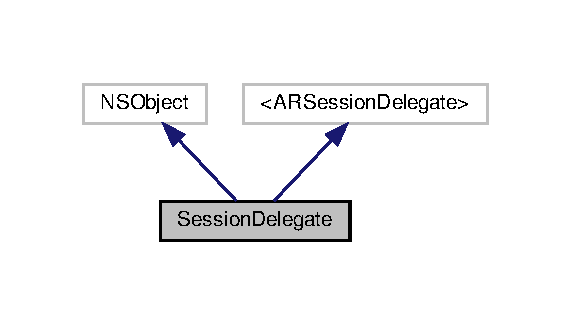
\includegraphics[width=288pt]{interfaceSessionDelegate__inherit__graph}
\end{center}
\end{figure}


Collaboration diagram for Session\+Delegate\+:
\nopagebreak
\begin{figure}[H]
\begin{center}
\leavevmode
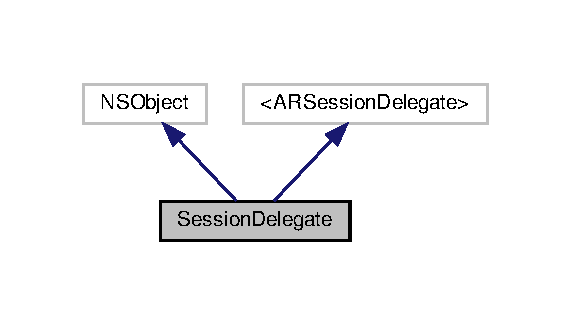
\includegraphics[width=288pt]{interfaceSessionDelegate__coll__graph}
\end{center}
\end{figure}
\doxysubsection*{Public Attributes}
\begin{DoxyCompactItemize}
\item 
\mbox{\Hypertarget{interfaceSessionDelegate_a205af00df48affe44122884199a506ad}\label{interfaceSessionDelegate_a205af00df48affe44122884199a506ad}} 
semaphore\+\_\+t {\bfseries \+\_\+semaphore}
\item 
\mbox{\Hypertarget{interfaceSessionDelegate_a80b6b669e67dc24266e00763029f3d97}\label{interfaceSessionDelegate_a80b6b669e67dc24266e00763029f3d97}} 
pthread\+\_\+mutex\+\_\+t {\bfseries \+\_\+mutex}
\item 
\mbox{\Hypertarget{interfaceSessionDelegate_ace9e7115174ecd921998eedee3defb4c}\label{interfaceSessionDelegate_ace9e7115174ecd921998eedee3defb4c}} 
C\+V\+Pixel\+Buffer\+Ref {\bfseries \+\_\+pixel\+Buffer}
\item 
\mbox{\Hypertarget{interfaceSessionDelegate_aad0cb30aed752a3ae50b17fc050fd214}\label{interfaceSessionDelegate_aad0cb30aed752a3ae50b17fc050fd214}} 
C\+V\+Pixel\+Buffer\+Ref {\bfseries \+\_\+depth\+Buffer}
\item 
\mbox{\Hypertarget{interfaceSessionDelegate_aca054d8eb1089ed57cef8fd6e1555f8d}\label{interfaceSessionDelegate_aca054d8eb1089ed57cef8fd6e1555f8d}} 
C\+V\+Pixel\+Buffer\+Ref {\bfseries \+\_\+confidence\+Buffer}
\item 
\mbox{\Hypertarget{interfaceSessionDelegate_a98e512d00bcac93d29618e6f2d6b9e36}\label{interfaceSessionDelegate_a98e512d00bcac93d29618e6f2d6b9e36}} 
unsigned long {\bfseries \+\_\+timestamp}
\end{DoxyCompactItemize}


The documentation for this class was generated from the following file\+:\begin{DoxyCompactItemize}
\item 
\mbox{\hyperlink{iphone__reader_8mm}{iphone\+\_\+reader.\+mm}}\end{DoxyCompactItemize}

\hypertarget{structmoetsi_1_1ssp_1_1SwsContextDeleter}{}\section{moetsi\+:\+:ssp\+:\+:Sws\+Context\+Deleter Struct Reference}
\label{structmoetsi_1_1ssp_1_1SwsContextDeleter}\index{moetsi\+::ssp\+::\+Sws\+Context\+Deleter@{moetsi\+::ssp\+::\+Sws\+Context\+Deleter}}
\subsection*{Public Member Functions}
\begin{DoxyCompactItemize}
\item 
\mbox{\Hypertarget{structmoetsi_1_1ssp_1_1SwsContextDeleter_a00a700e41e3ee79fdcffe1e0308315a6}\label{structmoetsi_1_1ssp_1_1SwsContextDeleter_a00a700e41e3ee79fdcffe1e0308315a6}} 
void {\bfseries operator()} (Sws\+Context $\ast$ptr) const
\end{DoxyCompactItemize}


The documentation for this struct was generated from the following file\+:\begin{DoxyCompactItemize}
\item 
libav\+\_\+types.\+h\end{DoxyCompactItemize}

\hypertarget{structUnityXRNativeSessionPtr}{}\doxysection{Unity\+X\+R\+Native\+Session\+Ptr Struct Reference}
\label{structUnityXRNativeSessionPtr}\index{UnityXRNativeSessionPtr@{UnityXRNativeSessionPtr}}
\doxysubsection*{Public Attributes}
\begin{DoxyCompactItemize}
\item 
\mbox{\Hypertarget{structUnityXRNativeSessionPtr_af9cb08b7c1666c1692eea15ee16cb636}\label{structUnityXRNativeSessionPtr_af9cb08b7c1666c1692eea15ee16cb636}} 
int {\bfseries version}
\item 
\mbox{\Hypertarget{structUnityXRNativeSessionPtr_a10991ea6b0b08a1ad91fe2fffb5de308}\label{structUnityXRNativeSessionPtr_a10991ea6b0b08a1ad91fe2fffb5de308}} 
void $\ast$ {\bfseries session}
\end{DoxyCompactItemize}


The documentation for this struct was generated from the following file\+:\begin{DoxyCompactItemize}
\item 
\mbox{\hyperlink{iphone__reader_8mm}{iphone\+\_\+reader.\+mm}}\end{DoxyCompactItemize}

\hypertarget{classmoetsi_1_1ssp_1_1VideoFileReader}{}\section{moetsi\+:\+:ssp\+:\+:Video\+File\+Reader Class Reference}
\label{classmoetsi_1_1ssp_1_1VideoFileReader}\index{moetsi\+::ssp\+::\+Video\+File\+Reader@{moetsi\+::ssp\+::\+Video\+File\+Reader}}


Inheritance diagram for moetsi\+:\+:ssp\+:\+:Video\+File\+Reader\+:
\nopagebreak
\begin{figure}[H]
\begin{center}
\leavevmode
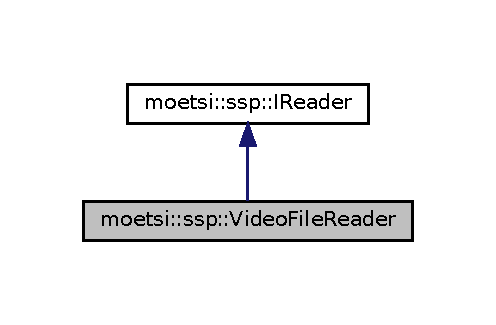
\includegraphics[width=226pt]{classmoetsi_1_1ssp_1_1VideoFileReader__inherit__graph}
\end{center}
\end{figure}


Collaboration diagram for moetsi\+:\+:ssp\+:\+:Video\+File\+Reader\+:
\nopagebreak
\begin{figure}[H]
\begin{center}
\leavevmode
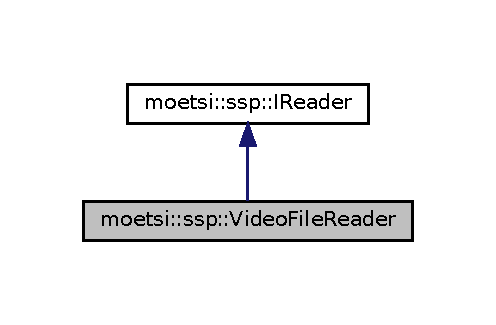
\includegraphics[width=226pt]{classmoetsi_1_1ssp_1_1VideoFileReader__coll__graph}
\end{center}
\end{figure}
\subsection*{Public Member Functions}
\begin{DoxyCompactItemize}
\item 
\mbox{\Hypertarget{classmoetsi_1_1ssp_1_1VideoFileReader_ab878eb4cdb141404d6860d5642157643}\label{classmoetsi_1_1ssp_1_1VideoFileReader_ab878eb4cdb141404d6860d5642157643}} 
{\bfseries Video\+File\+Reader} (std\+::string \&filename)
\item 
\mbox{\Hypertarget{classmoetsi_1_1ssp_1_1VideoFileReader_a1d13ddb9bea806a1dbf8da68a1f4318b}\label{classmoetsi_1_1ssp_1_1VideoFileReader_a1d13ddb9bea806a1dbf8da68a1f4318b}} 
{\bfseries Video\+File\+Reader} (std\+::string \&filename, std\+::vector$<$ unsigned int $>$ \&video\+\_\+stream\+\_\+indexes)
\item 
\mbox{\Hypertarget{classmoetsi_1_1ssp_1_1VideoFileReader_a1c4adbf0de8d00d52b36fade1f30baa4}\label{classmoetsi_1_1ssp_1_1VideoFileReader_a1c4adbf0de8d00d52b36fade1f30baa4}} 
virtual std\+::vector$<$ std\+::shared\+\_\+ptr$<$ \hyperlink{structmoetsi_1_1ssp_1_1FrameStruct}{Frame\+Struct} $>$ $>$ \hyperlink{classmoetsi_1_1ssp_1_1VideoFileReader_a1c4adbf0de8d00d52b36fade1f30baa4}{Get\+Current\+Frame} ()
\begin{DoxyCompactList}\small\item\em Get current frame data. \end{DoxyCompactList}\item 
virtual std\+::vector$<$ \hyperlink{namespacemoetsi_1_1ssp_a46efdfa2cd5a28ead465dcc8006b5a87}{Frame\+Type} $>$ \hyperlink{classmoetsi_1_1ssp_1_1VideoFileReader_a9d47af47299c5fccf766ac2d848a561b}{Get\+Type} ()
\begin{DoxyCompactList}\small\item\em Get frame types. \end{DoxyCompactList}\item 
virtual bool \hyperlink{classmoetsi_1_1ssp_1_1VideoFileReader_ab5733b56b6d6dd7596eac9d914481c7e}{Has\+Next\+Frame} ()
\begin{DoxyCompactList}\small\item\em Check if there is a next frame. \end{DoxyCompactList}\item 
\mbox{\Hypertarget{classmoetsi_1_1ssp_1_1VideoFileReader_afdaf5606fd0cfcc2e1b5b7c0fb271ebf}\label{classmoetsi_1_1ssp_1_1VideoFileReader_afdaf5606fd0cfcc2e1b5b7c0fb271ebf}} 
virtual void \hyperlink{classmoetsi_1_1ssp_1_1VideoFileReader_afdaf5606fd0cfcc2e1b5b7c0fb271ebf}{Next\+Frame} ()
\begin{DoxyCompactList}\small\item\em Go to next frame. \end{DoxyCompactList}\item 
\mbox{\Hypertarget{classmoetsi_1_1ssp_1_1VideoFileReader_ac646d10b57d4e3b3ff4d1c83a47e8c3d}\label{classmoetsi_1_1ssp_1_1VideoFileReader_ac646d10b57d4e3b3ff4d1c83a47e8c3d}} 
virtual void \hyperlink{classmoetsi_1_1ssp_1_1VideoFileReader_ac646d10b57d4e3b3ff4d1c83a47e8c3d}{Reset} ()
\begin{DoxyCompactList}\small\item\em Reset this reader. \end{DoxyCompactList}\item 
virtual void \hyperlink{classmoetsi_1_1ssp_1_1VideoFileReader_ad98a532db8b1e2c3879df274b2efb082}{Go\+To\+Frame} (unsigned int frame\+\_\+id)
\begin{DoxyCompactList}\small\item\em Go to a given frame. \end{DoxyCompactList}\item 
virtual unsigned int \hyperlink{classmoetsi_1_1ssp_1_1VideoFileReader_aef5c92da2645cddc7e4ffcfd34ad4b8a}{Get\+Current\+Frame\+Id} ()
\begin{DoxyCompactList}\small\item\em Get current frame number. \end{DoxyCompactList}\item 
virtual unsigned int \hyperlink{classmoetsi_1_1ssp_1_1VideoFileReader_a83359ad82898acdb75240568b182247c}{Get\+Fps} ()
\begin{DoxyCompactList}\small\item\em Get indicative F\+PS in frame per second. \end{DoxyCompactList}\end{DoxyCompactItemize}


\subsection{Member Function Documentation}
\mbox{\Hypertarget{classmoetsi_1_1ssp_1_1VideoFileReader_aef5c92da2645cddc7e4ffcfd34ad4b8a}\label{classmoetsi_1_1ssp_1_1VideoFileReader_aef5c92da2645cddc7e4ffcfd34ad4b8a}} 
\index{moetsi\+::ssp\+::\+Video\+File\+Reader@{moetsi\+::ssp\+::\+Video\+File\+Reader}!Get\+Current\+Frame\+Id@{Get\+Current\+Frame\+Id}}
\index{Get\+Current\+Frame\+Id@{Get\+Current\+Frame\+Id}!moetsi\+::ssp\+::\+Video\+File\+Reader@{moetsi\+::ssp\+::\+Video\+File\+Reader}}
\subsubsection{\texorpdfstring{Get\+Current\+Frame\+Id()}{GetCurrentFrameId()}}
{\footnotesize\ttfamily unsigned int moetsi\+::ssp\+::\+Video\+File\+Reader\+::\+Get\+Current\+Frame\+Id (\begin{DoxyParamCaption}{ }\end{DoxyParamCaption})\hspace{0.3cm}{\ttfamily [virtual]}}



Get current frame number. 

\begin{DoxyReturn}{Returns}
current frame number. 
\end{DoxyReturn}


Implements \hyperlink{classmoetsi_1_1ssp_1_1IReader_ac292d83eb06dee277baaa06e281a562d}{moetsi\+::ssp\+::\+I\+Reader}.

\mbox{\Hypertarget{classmoetsi_1_1ssp_1_1VideoFileReader_a83359ad82898acdb75240568b182247c}\label{classmoetsi_1_1ssp_1_1VideoFileReader_a83359ad82898acdb75240568b182247c}} 
\index{moetsi\+::ssp\+::\+Video\+File\+Reader@{moetsi\+::ssp\+::\+Video\+File\+Reader}!Get\+Fps@{Get\+Fps}}
\index{Get\+Fps@{Get\+Fps}!moetsi\+::ssp\+::\+Video\+File\+Reader@{moetsi\+::ssp\+::\+Video\+File\+Reader}}
\subsubsection{\texorpdfstring{Get\+Fps()}{GetFps()}}
{\footnotesize\ttfamily unsigned int moetsi\+::ssp\+::\+Video\+File\+Reader\+::\+Get\+Fps (\begin{DoxyParamCaption}{ }\end{DoxyParamCaption})\hspace{0.3cm}{\ttfamily [virtual]}}



Get indicative F\+PS in frame per second. 

\begin{DoxyReturn}{Returns}
the F\+PS number 
\end{DoxyReturn}


Implements \hyperlink{classmoetsi_1_1ssp_1_1IReader_a9f6a8650ca290b011b8e5451eeae9f32}{moetsi\+::ssp\+::\+I\+Reader}.

\mbox{\Hypertarget{classmoetsi_1_1ssp_1_1VideoFileReader_a9d47af47299c5fccf766ac2d848a561b}\label{classmoetsi_1_1ssp_1_1VideoFileReader_a9d47af47299c5fccf766ac2d848a561b}} 
\index{moetsi\+::ssp\+::\+Video\+File\+Reader@{moetsi\+::ssp\+::\+Video\+File\+Reader}!Get\+Type@{Get\+Type}}
\index{Get\+Type@{Get\+Type}!moetsi\+::ssp\+::\+Video\+File\+Reader@{moetsi\+::ssp\+::\+Video\+File\+Reader}}
\subsubsection{\texorpdfstring{Get\+Type()}{GetType()}}
{\footnotesize\ttfamily std\+::vector$<$ \hyperlink{namespacemoetsi_1_1ssp_a46efdfa2cd5a28ead465dcc8006b5a87}{Frame\+Type} $>$ moetsi\+::ssp\+::\+Video\+File\+Reader\+::\+Get\+Type (\begin{DoxyParamCaption}{ }\end{DoxyParamCaption})\hspace{0.3cm}{\ttfamily [virtual]}}



Get frame types. 

\begin{DoxyReturn}{Returns}
a vector of Frame\+Type, listing available data types 
\end{DoxyReturn}


Implements \hyperlink{classmoetsi_1_1ssp_1_1IReader_a4116c1931fde7bd66133934ffdca1cce}{moetsi\+::ssp\+::\+I\+Reader}.

\mbox{\Hypertarget{classmoetsi_1_1ssp_1_1VideoFileReader_ad98a532db8b1e2c3879df274b2efb082}\label{classmoetsi_1_1ssp_1_1VideoFileReader_ad98a532db8b1e2c3879df274b2efb082}} 
\index{moetsi\+::ssp\+::\+Video\+File\+Reader@{moetsi\+::ssp\+::\+Video\+File\+Reader}!Go\+To\+Frame@{Go\+To\+Frame}}
\index{Go\+To\+Frame@{Go\+To\+Frame}!moetsi\+::ssp\+::\+Video\+File\+Reader@{moetsi\+::ssp\+::\+Video\+File\+Reader}}
\subsubsection{\texorpdfstring{Go\+To\+Frame()}{GoToFrame()}}
{\footnotesize\ttfamily void moetsi\+::ssp\+::\+Video\+File\+Reader\+::\+Go\+To\+Frame (\begin{DoxyParamCaption}\item[{unsigned int}]{frame\+\_\+id }\end{DoxyParamCaption})\hspace{0.3cm}{\ttfamily [virtual]}}



Go to a given frame. 


\begin{DoxyParams}{Parameters}
{\em frame\+\_\+id} & target frame number \\
\hline
\end{DoxyParams}


Implements \hyperlink{classmoetsi_1_1ssp_1_1IReader_a6f1be3c06538992cca6d550bd9566681}{moetsi\+::ssp\+::\+I\+Reader}.

\mbox{\Hypertarget{classmoetsi_1_1ssp_1_1VideoFileReader_ab5733b56b6d6dd7596eac9d914481c7e}\label{classmoetsi_1_1ssp_1_1VideoFileReader_ab5733b56b6d6dd7596eac9d914481c7e}} 
\index{moetsi\+::ssp\+::\+Video\+File\+Reader@{moetsi\+::ssp\+::\+Video\+File\+Reader}!Has\+Next\+Frame@{Has\+Next\+Frame}}
\index{Has\+Next\+Frame@{Has\+Next\+Frame}!moetsi\+::ssp\+::\+Video\+File\+Reader@{moetsi\+::ssp\+::\+Video\+File\+Reader}}
\subsubsection{\texorpdfstring{Has\+Next\+Frame()}{HasNextFrame()}}
{\footnotesize\ttfamily bool moetsi\+::ssp\+::\+Video\+File\+Reader\+::\+Has\+Next\+Frame (\begin{DoxyParamCaption}{ }\end{DoxyParamCaption})\hspace{0.3cm}{\ttfamily [virtual]}}



Check if there is a next frame. 

\begin{DoxyReturn}{Returns}
true if there is a next frame 
\end{DoxyReturn}


Implements \hyperlink{classmoetsi_1_1ssp_1_1IReader_af9186ba41e136dc4ec3242b5dd55fa04}{moetsi\+::ssp\+::\+I\+Reader}.



The documentation for this class was generated from the following files\+:\begin{DoxyCompactItemize}
\item 
\hyperlink{video__file__reader_8h}{video\+\_\+file\+\_\+reader.\+h}\item 
\hyperlink{video__file__reader_8cc}{video\+\_\+file\+\_\+reader.\+cc}\end{DoxyCompactItemize}

\hypertarget{classmoetsi_1_1ssp_1_1ZDepthDecoder}{}\doxysection{moetsi\+::ssp\+::Z\+Depth\+Decoder Class Reference}
\label{classmoetsi_1_1ssp_1_1ZDepthDecoder}\index{moetsi::ssp::ZDepthDecoder@{moetsi::ssp::ZDepthDecoder}}


\mbox{\hyperlink{classmoetsi_1_1ssp_1_1ZDepthDecoder}{Z\+Depth\+Decoder}} Z\+Depth format decoder.  




{\ttfamily \#include $<$zdepth\+\_\+decoder.\+h$>$}



Inheritance diagram for moetsi\+::ssp\+::Z\+Depth\+Decoder\+:
\nopagebreak
\begin{figure}[H]
\begin{center}
\leavevmode
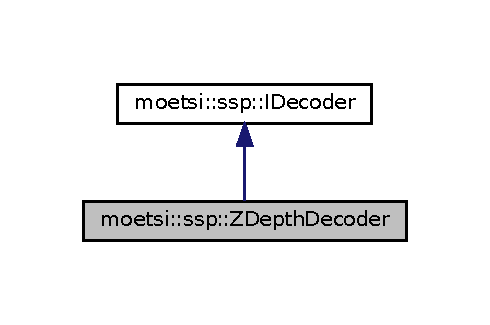
\includegraphics[width=235pt]{classmoetsi_1_1ssp_1_1ZDepthDecoder__inherit__graph}
\end{center}
\end{figure}


Collaboration diagram for moetsi\+::ssp\+::Z\+Depth\+Decoder\+:
\nopagebreak
\begin{figure}[H]
\begin{center}
\leavevmode
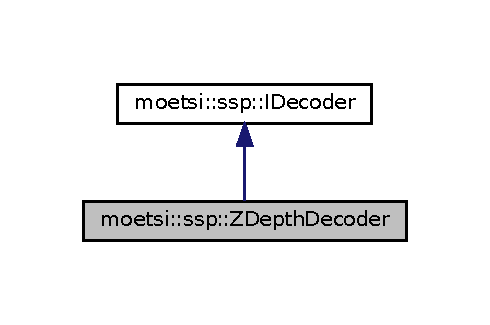
\includegraphics[width=235pt]{classmoetsi_1_1ssp_1_1ZDepthDecoder__coll__graph}
\end{center}
\end{figure}
\doxysubsection*{Public Member Functions}
\begin{DoxyCompactItemize}
\item 
\mbox{\Hypertarget{classmoetsi_1_1ssp_1_1ZDepthDecoder_a69f45e16839baaa30da870efbfb48101}\label{classmoetsi_1_1ssp_1_1ZDepthDecoder_a69f45e16839baaa30da870efbfb48101}} 
\mbox{\hyperlink{classmoetsi_1_1ssp_1_1ZDepthDecoder_a69f45e16839baaa30da870efbfb48101}{Z\+Depth\+Decoder}} ()
\begin{DoxyCompactList}\small\item\em Constructor. \end{DoxyCompactList}\item 
\mbox{\Hypertarget{classmoetsi_1_1ssp_1_1ZDepthDecoder_ae189577c97401e787d240c9854d83661}\label{classmoetsi_1_1ssp_1_1ZDepthDecoder_ae189577c97401e787d240c9854d83661}} 
\mbox{\hyperlink{classmoetsi_1_1ssp_1_1ZDepthDecoder_ae189577c97401e787d240c9854d83661}{$\sim$\+Z\+Depth\+Decoder}} ()
\begin{DoxyCompactList}\small\item\em Destructor. \end{DoxyCompactList}\item 
void \mbox{\hyperlink{classmoetsi_1_1ssp_1_1ZDepthDecoder_aad7fe4789b709fc3496a1837a8ff86e5}{Init}} (std\+::vector$<$ unsigned char $>$ parameter\+\_\+data)
\begin{DoxyCompactList}\small\item\em Initialize. \end{DoxyCompactList}\item 
cv\+::\+Mat \mbox{\hyperlink{classmoetsi_1_1ssp_1_1ZDepthDecoder_a43226095658d616f7e38df1d43c2f88a}{Decode}} (\mbox{\hyperlink{structmoetsi_1_1ssp_1_1FrameStruct}{Frame\+Struct}} \&frame)
\begin{DoxyCompactList}\small\item\em Extract an opencv image from a \mbox{\hyperlink{structmoetsi_1_1ssp_1_1FrameStruct}{Frame\+Struct}}. \end{DoxyCompactList}\end{DoxyCompactItemize}


\doxysubsection{Detailed Description}
\mbox{\hyperlink{classmoetsi_1_1ssp_1_1ZDepthDecoder}{Z\+Depth\+Decoder}} Z\+Depth format decoder. 

\doxysubsection{Member Function Documentation}
\mbox{\Hypertarget{classmoetsi_1_1ssp_1_1ZDepthDecoder_a43226095658d616f7e38df1d43c2f88a}\label{classmoetsi_1_1ssp_1_1ZDepthDecoder_a43226095658d616f7e38df1d43c2f88a}} 
\index{moetsi::ssp::ZDepthDecoder@{moetsi::ssp::ZDepthDecoder}!Decode@{Decode}}
\index{Decode@{Decode}!moetsi::ssp::ZDepthDecoder@{moetsi::ssp::ZDepthDecoder}}
\doxysubsubsection{\texorpdfstring{Decode()}{Decode()}}
{\footnotesize\ttfamily cv\+::\+Mat moetsi\+::ssp\+::\+Z\+Depth\+Decoder\+::\+Decode (\begin{DoxyParamCaption}\item[{\mbox{\hyperlink{structmoetsi_1_1ssp_1_1FrameStruct}{Frame\+Struct}} \&}]{frame }\end{DoxyParamCaption})\hspace{0.3cm}{\ttfamily [virtual]}}



Extract an opencv image from a \mbox{\hyperlink{structmoetsi_1_1ssp_1_1FrameStruct}{Frame\+Struct}}. 


\begin{DoxyParams}{Parameters}
{\em data} & \mbox{\hyperlink{structmoetsi_1_1ssp_1_1FrameStruct}{Frame\+Struct}} \\
\hline
\end{DoxyParams}
\begin{DoxyReturn}{Returns}
Open\+CV matrix/image 
\end{DoxyReturn}


Implements \mbox{\hyperlink{classmoetsi_1_1ssp_1_1IDecoder_a1c06604dc4107d3668a4e791c13cc063}{moetsi\+::ssp\+::\+I\+Decoder}}.

\mbox{\Hypertarget{classmoetsi_1_1ssp_1_1ZDepthDecoder_aad7fe4789b709fc3496a1837a8ff86e5}\label{classmoetsi_1_1ssp_1_1ZDepthDecoder_aad7fe4789b709fc3496a1837a8ff86e5}} 
\index{moetsi::ssp::ZDepthDecoder@{moetsi::ssp::ZDepthDecoder}!Init@{Init}}
\index{Init@{Init}!moetsi::ssp::ZDepthDecoder@{moetsi::ssp::ZDepthDecoder}}
\doxysubsubsection{\texorpdfstring{Init()}{Init()}}
{\footnotesize\ttfamily void moetsi\+::ssp\+::\+Z\+Depth\+Decoder\+::\+Init (\begin{DoxyParamCaption}\item[{std\+::vector$<$ unsigned char $>$}]{parameter\+\_\+data }\end{DoxyParamCaption})}



Initialize. 


\begin{DoxyParams}{Parameters}
{\em parameter\+\_\+data} & parameters \\
\hline
\end{DoxyParams}


The documentation for this class was generated from the following files\+:\begin{DoxyCompactItemize}
\item 
\mbox{\hyperlink{zdepth__decoder_8h}{zdepth\+\_\+decoder.\+h}}\item 
\mbox{\hyperlink{zdepth__decoder_8cc}{zdepth\+\_\+decoder.\+cc}}\end{DoxyCompactItemize}

\hypertarget{classmoetsi_1_1ssp_1_1ZDepthEncoder}{}\section{moetsi\+:\+:ssp\+:\+:Z\+Depth\+Encoder Class Reference}
\label{classmoetsi_1_1ssp_1_1ZDepthEncoder}\index{moetsi\+::ssp\+::\+Z\+Depth\+Encoder@{moetsi\+::ssp\+::\+Z\+Depth\+Encoder}}


Z\+Depth encoder.  




{\ttfamily \#include $<$zdepth\+\_\+encoder.\+h$>$}



Inheritance diagram for moetsi\+:\+:ssp\+:\+:Z\+Depth\+Encoder\+:
\nopagebreak
\begin{figure}[H]
\begin{center}
\leavevmode
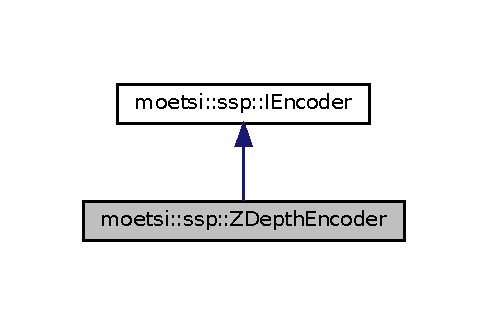
\includegraphics[width=222pt]{classmoetsi_1_1ssp_1_1ZDepthEncoder__inherit__graph}
\end{center}
\end{figure}


Collaboration diagram for moetsi\+:\+:ssp\+:\+:Z\+Depth\+Encoder\+:
\nopagebreak
\begin{figure}[H]
\begin{center}
\leavevmode
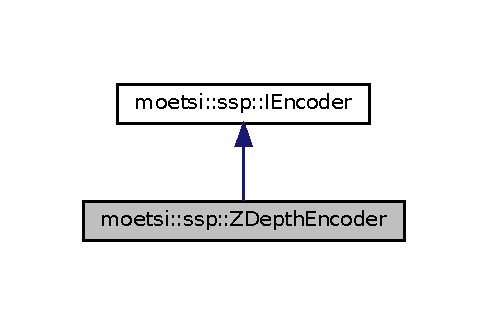
\includegraphics[width=222pt]{classmoetsi_1_1ssp_1_1ZDepthEncoder__coll__graph}
\end{center}
\end{figure}
\subsection*{Public Member Functions}
\begin{DoxyCompactItemize}
\item 
\hyperlink{classmoetsi_1_1ssp_1_1ZDepthEncoder_a97902734a32136d68782f4b8c9bf111c}{Z\+Depth\+Encoder} (Y\+A\+M\+L\+::\+Node \&\+\_\+codec\+\_\+parameters, int \+\_\+fps)
\begin{DoxyCompactList}\small\item\em Constructor. \end{DoxyCompactList}\item 
\mbox{\Hypertarget{classmoetsi_1_1ssp_1_1ZDepthEncoder_ae668b2baffa6d7debb78608f488cd466}\label{classmoetsi_1_1ssp_1_1ZDepthEncoder_ae668b2baffa6d7debb78608f488cd466}} 
\hyperlink{classmoetsi_1_1ssp_1_1ZDepthEncoder_ae668b2baffa6d7debb78608f488cd466}{$\sim$\+Z\+Depth\+Encoder} ()
\begin{DoxyCompactList}\small\item\em Destructor. \end{DoxyCompactList}\item 
virtual void \hyperlink{classmoetsi_1_1ssp_1_1ZDepthEncoder_a382e94eab7789cb4437b9711e5292343}{Add\+Frame\+Struct} (std\+::shared\+\_\+ptr$<$ \hyperlink{structmoetsi_1_1ssp_1_1FrameStruct}{Frame\+Struct} $>$ \&frame\+\_\+struct)
\begin{DoxyCompactList}\small\item\em Add a frame struct. \end{DoxyCompactList}\item 
\mbox{\Hypertarget{classmoetsi_1_1ssp_1_1ZDepthEncoder_ae3911f396fc8b86c04c94dc71e1c0672}\label{classmoetsi_1_1ssp_1_1ZDepthEncoder_ae3911f396fc8b86c04c94dc71e1c0672}} 
virtual void \hyperlink{classmoetsi_1_1ssp_1_1ZDepthEncoder_ae3911f396fc8b86c04c94dc71e1c0672}{Next\+Packet} ()
\begin{DoxyCompactList}\small\item\em Go to next packet. \end{DoxyCompactList}\item 
virtual bool \hyperlink{classmoetsi_1_1ssp_1_1ZDepthEncoder_ac11aa1369150c2aa5ffa1d70d4e6ad5d}{Has\+Next\+Packet} ()
\begin{DoxyCompactList}\small\item\em Check if there is a next packet. \end{DoxyCompactList}\item 
virtual std\+::shared\+\_\+ptr$<$ \hyperlink{structmoetsi_1_1ssp_1_1FrameStruct}{Frame\+Struct} $>$ \hyperlink{classmoetsi_1_1ssp_1_1ZDepthEncoder_a075752f62bbc40f71026812c5548ef5f}{Current\+Frame\+Encoded} ()
\begin{DoxyCompactList}\small\item\em Get current encoded frame. \end{DoxyCompactList}\item 
virtual std\+::shared\+\_\+ptr$<$ \hyperlink{structmoetsi_1_1ssp_1_1FrameStruct}{Frame\+Struct} $>$ \hyperlink{classmoetsi_1_1ssp_1_1ZDepthEncoder_abe5820ee0dea5fec22e398a7ba4d6777}{Current\+Frame\+Original} ()
\begin{DoxyCompactList}\small\item\em Get current frame in its original format. \end{DoxyCompactList}\item 
virtual std\+::shared\+\_\+ptr$<$ \hyperlink{structmoetsi_1_1ssp_1_1CodecParamsStruct}{Codec\+Params\+Struct} $>$ \hyperlink{classmoetsi_1_1ssp_1_1ZDepthEncoder_a3fc9f84387dba09d1deb4761031b598f}{Get\+Codec\+Params\+Struct} ()
\begin{DoxyCompactList}\small\item\em Get codec parameters. \end{DoxyCompactList}\item 
virtual unsigned int \hyperlink{classmoetsi_1_1ssp_1_1ZDepthEncoder_a9ea0a5783d7d265fccc3a2c262600552}{Get\+Fps} ()
\begin{DoxyCompactList}\small\item\em Get F\+PS. \end{DoxyCompactList}\end{DoxyCompactItemize}


\subsection{Detailed Description}
Z\+Depth encoder. 

\subsection{Constructor \& Destructor Documentation}
\mbox{\Hypertarget{classmoetsi_1_1ssp_1_1ZDepthEncoder_a97902734a32136d68782f4b8c9bf111c}\label{classmoetsi_1_1ssp_1_1ZDepthEncoder_a97902734a32136d68782f4b8c9bf111c}} 
\index{moetsi\+::ssp\+::\+Z\+Depth\+Encoder@{moetsi\+::ssp\+::\+Z\+Depth\+Encoder}!Z\+Depth\+Encoder@{Z\+Depth\+Encoder}}
\index{Z\+Depth\+Encoder@{Z\+Depth\+Encoder}!moetsi\+::ssp\+::\+Z\+Depth\+Encoder@{moetsi\+::ssp\+::\+Z\+Depth\+Encoder}}
\subsubsection{\texorpdfstring{Z\+Depth\+Encoder()}{ZDepthEncoder()}}
{\footnotesize\ttfamily moetsi\+::ssp\+::\+Z\+Depth\+Encoder\+::\+Z\+Depth\+Encoder (\begin{DoxyParamCaption}\item[{Y\+A\+M\+L\+::\+Node \&}]{\+\_\+codec\+\_\+parameters,  }\item[{int}]{\+\_\+fps }\end{DoxyParamCaption})}



Constructor. 


\begin{DoxyParams}{Parameters}
{\em \+\_\+codec\+\_\+parameters} & \\
\hline
{\em \+\_\+fps} & Frame per second \\
\hline
\end{DoxyParams}


\subsection{Member Function Documentation}
\mbox{\Hypertarget{classmoetsi_1_1ssp_1_1ZDepthEncoder_a382e94eab7789cb4437b9711e5292343}\label{classmoetsi_1_1ssp_1_1ZDepthEncoder_a382e94eab7789cb4437b9711e5292343}} 
\index{moetsi\+::ssp\+::\+Z\+Depth\+Encoder@{moetsi\+::ssp\+::\+Z\+Depth\+Encoder}!Add\+Frame\+Struct@{Add\+Frame\+Struct}}
\index{Add\+Frame\+Struct@{Add\+Frame\+Struct}!moetsi\+::ssp\+::\+Z\+Depth\+Encoder@{moetsi\+::ssp\+::\+Z\+Depth\+Encoder}}
\subsubsection{\texorpdfstring{Add\+Frame\+Struct()}{AddFrameStruct()}}
{\footnotesize\ttfamily void moetsi\+::ssp\+::\+Z\+Depth\+Encoder\+::\+Add\+Frame\+Struct (\begin{DoxyParamCaption}\item[{std\+::shared\+\_\+ptr$<$ \hyperlink{structmoetsi_1_1ssp_1_1FrameStruct}{Frame\+Struct} $>$ \&}]{frame\+\_\+struct }\end{DoxyParamCaption})\hspace{0.3cm}{\ttfamily [virtual]}}



Add a frame struct. 


\begin{DoxyParams}{Parameters}
{\em frame\+\_\+struct} & \hyperlink{structmoetsi_1_1ssp_1_1FrameStruct}{Frame\+Struct} to add \\
\hline
\end{DoxyParams}


Implements \hyperlink{classmoetsi_1_1ssp_1_1IEncoder_a8c223ec82fdd30ee8ee75157306054ec}{moetsi\+::ssp\+::\+I\+Encoder}.

\mbox{\Hypertarget{classmoetsi_1_1ssp_1_1ZDepthEncoder_a075752f62bbc40f71026812c5548ef5f}\label{classmoetsi_1_1ssp_1_1ZDepthEncoder_a075752f62bbc40f71026812c5548ef5f}} 
\index{moetsi\+::ssp\+::\+Z\+Depth\+Encoder@{moetsi\+::ssp\+::\+Z\+Depth\+Encoder}!Current\+Frame\+Encoded@{Current\+Frame\+Encoded}}
\index{Current\+Frame\+Encoded@{Current\+Frame\+Encoded}!moetsi\+::ssp\+::\+Z\+Depth\+Encoder@{moetsi\+::ssp\+::\+Z\+Depth\+Encoder}}
\subsubsection{\texorpdfstring{Current\+Frame\+Encoded()}{CurrentFrameEncoded()}}
{\footnotesize\ttfamily std\+::shared\+\_\+ptr$<$ \hyperlink{structmoetsi_1_1ssp_1_1FrameStruct}{Frame\+Struct} $>$ moetsi\+::ssp\+::\+Z\+Depth\+Encoder\+::\+Current\+Frame\+Encoded (\begin{DoxyParamCaption}{ }\end{DoxyParamCaption})\hspace{0.3cm}{\ttfamily [virtual]}}



Get current encoded frame. 

\begin{DoxyReturn}{Returns}
current encoded frame 
\end{DoxyReturn}


Implements \hyperlink{classmoetsi_1_1ssp_1_1IEncoder_a178d117518e7c7007414ea9c82bd3ed6}{moetsi\+::ssp\+::\+I\+Encoder}.

\mbox{\Hypertarget{classmoetsi_1_1ssp_1_1ZDepthEncoder_abe5820ee0dea5fec22e398a7ba4d6777}\label{classmoetsi_1_1ssp_1_1ZDepthEncoder_abe5820ee0dea5fec22e398a7ba4d6777}} 
\index{moetsi\+::ssp\+::\+Z\+Depth\+Encoder@{moetsi\+::ssp\+::\+Z\+Depth\+Encoder}!Current\+Frame\+Original@{Current\+Frame\+Original}}
\index{Current\+Frame\+Original@{Current\+Frame\+Original}!moetsi\+::ssp\+::\+Z\+Depth\+Encoder@{moetsi\+::ssp\+::\+Z\+Depth\+Encoder}}
\subsubsection{\texorpdfstring{Current\+Frame\+Original()}{CurrentFrameOriginal()}}
{\footnotesize\ttfamily std\+::shared\+\_\+ptr$<$ \hyperlink{structmoetsi_1_1ssp_1_1FrameStruct}{Frame\+Struct} $>$ moetsi\+::ssp\+::\+Z\+Depth\+Encoder\+::\+Current\+Frame\+Original (\begin{DoxyParamCaption}{ }\end{DoxyParamCaption})\hspace{0.3cm}{\ttfamily [virtual]}}



Get current frame in its original format. 

\begin{DoxyReturn}{Returns}
current frame in its original format 
\end{DoxyReturn}


Implements \hyperlink{classmoetsi_1_1ssp_1_1IEncoder_ab60bdaae0a85289dfa31a12bab533dc0}{moetsi\+::ssp\+::\+I\+Encoder}.

\mbox{\Hypertarget{classmoetsi_1_1ssp_1_1ZDepthEncoder_a3fc9f84387dba09d1deb4761031b598f}\label{classmoetsi_1_1ssp_1_1ZDepthEncoder_a3fc9f84387dba09d1deb4761031b598f}} 
\index{moetsi\+::ssp\+::\+Z\+Depth\+Encoder@{moetsi\+::ssp\+::\+Z\+Depth\+Encoder}!Get\+Codec\+Params\+Struct@{Get\+Codec\+Params\+Struct}}
\index{Get\+Codec\+Params\+Struct@{Get\+Codec\+Params\+Struct}!moetsi\+::ssp\+::\+Z\+Depth\+Encoder@{moetsi\+::ssp\+::\+Z\+Depth\+Encoder}}
\subsubsection{\texorpdfstring{Get\+Codec\+Params\+Struct()}{GetCodecParamsStruct()}}
{\footnotesize\ttfamily std\+::shared\+\_\+ptr$<$ \hyperlink{structmoetsi_1_1ssp_1_1CodecParamsStruct}{Codec\+Params\+Struct} $>$ moetsi\+::ssp\+::\+Z\+Depth\+Encoder\+::\+Get\+Codec\+Params\+Struct (\begin{DoxyParamCaption}{ }\end{DoxyParamCaption})\hspace{0.3cm}{\ttfamily [virtual]}}



Get codec parameters. 

\begin{DoxyReturn}{Returns}
codec parameters 
\end{DoxyReturn}


Implements \hyperlink{classmoetsi_1_1ssp_1_1IEncoder_ad5179efaa4c74207766dd64f46f4059a}{moetsi\+::ssp\+::\+I\+Encoder}.

\mbox{\Hypertarget{classmoetsi_1_1ssp_1_1ZDepthEncoder_a9ea0a5783d7d265fccc3a2c262600552}\label{classmoetsi_1_1ssp_1_1ZDepthEncoder_a9ea0a5783d7d265fccc3a2c262600552}} 
\index{moetsi\+::ssp\+::\+Z\+Depth\+Encoder@{moetsi\+::ssp\+::\+Z\+Depth\+Encoder}!Get\+Fps@{Get\+Fps}}
\index{Get\+Fps@{Get\+Fps}!moetsi\+::ssp\+::\+Z\+Depth\+Encoder@{moetsi\+::ssp\+::\+Z\+Depth\+Encoder}}
\subsubsection{\texorpdfstring{Get\+Fps()}{GetFps()}}
{\footnotesize\ttfamily unsigned int moetsi\+::ssp\+::\+Z\+Depth\+Encoder\+::\+Get\+Fps (\begin{DoxyParamCaption}{ }\end{DoxyParamCaption})\hspace{0.3cm}{\ttfamily [virtual]}}



Get F\+PS. 

\begin{DoxyReturn}{Returns}
F\+PS in frame per second 
\end{DoxyReturn}


Implements \hyperlink{classmoetsi_1_1ssp_1_1IEncoder_ae6a865aa52230d81aed1cb5232402f6c}{moetsi\+::ssp\+::\+I\+Encoder}.

\mbox{\Hypertarget{classmoetsi_1_1ssp_1_1ZDepthEncoder_ac11aa1369150c2aa5ffa1d70d4e6ad5d}\label{classmoetsi_1_1ssp_1_1ZDepthEncoder_ac11aa1369150c2aa5ffa1d70d4e6ad5d}} 
\index{moetsi\+::ssp\+::\+Z\+Depth\+Encoder@{moetsi\+::ssp\+::\+Z\+Depth\+Encoder}!Has\+Next\+Packet@{Has\+Next\+Packet}}
\index{Has\+Next\+Packet@{Has\+Next\+Packet}!moetsi\+::ssp\+::\+Z\+Depth\+Encoder@{moetsi\+::ssp\+::\+Z\+Depth\+Encoder}}
\subsubsection{\texorpdfstring{Has\+Next\+Packet()}{HasNextPacket()}}
{\footnotesize\ttfamily bool moetsi\+::ssp\+::\+Z\+Depth\+Encoder\+::\+Has\+Next\+Packet (\begin{DoxyParamCaption}{ }\end{DoxyParamCaption})\hspace{0.3cm}{\ttfamily [virtual]}}



Check if there is a next packet. 

\begin{DoxyReturn}{Returns}
true if there is a next packet 
\end{DoxyReturn}


Implements \hyperlink{classmoetsi_1_1ssp_1_1IEncoder_a2af8e23d841ef61f6ee4037e56a3694d}{moetsi\+::ssp\+::\+I\+Encoder}.



The documentation for this class was generated from the following files\+:\begin{DoxyCompactItemize}
\item 
\hyperlink{zdepth__encoder_8h}{zdepth\+\_\+encoder.\+h}\item 
\hyperlink{zdepth__encoder_8cc}{zdepth\+\_\+encoder.\+cc}\end{DoxyCompactItemize}

\chapter{File Documentation}
\hypertarget{dummy__body__reader_8cc}{}\doxysection{dummy\+\_\+body\+\_\+reader.\+cc File Reference}
\label{dummy__body__reader_8cc}\index{dummy\_body\_reader.cc@{dummy\_body\_reader.cc}}


Dumy Body Reader.  


{\ttfamily \#include \char`\"{}dummy\+\_\+body\+\_\+reader.\+h\char`\"{}}\newline
Include dependency graph for dummy\+\_\+body\+\_\+reader.\+cc\+:
% FIG 0
\doxysubsection*{Namespaces}
\begin{DoxyCompactItemize}
\item 
 \mbox{\hyperlink{namespacemoetsi}{moetsi}}
\begin{DoxyCompactList}\small\item\em Moetsi creations. \end{DoxyCompactList}\item 
 \mbox{\hyperlink{namespacemoetsi_1_1ssp}{moetsi\+::ssp}}
\begin{DoxyCompactList}\small\item\em Sensor Stream Pipe. \end{DoxyCompactList}\end{DoxyCompactItemize}


\doxysubsection{Detailed Description}
Dumy Body Reader. 


\hypertarget{dummy__body__reader_8h}{}\section{dummy\+\_\+body\+\_\+reader.\+h File Reference}
\label{dummy__body__reader_8h}\index{dummy\+\_\+body\+\_\+reader.\+h@{dummy\+\_\+body\+\_\+reader.\+h}}


Dumy Body Reader.  


{\ttfamily \#include $<$atomic$>$}\newline
{\ttfamily \#include $<$fstream$>$}\newline
{\ttfamily \#include $<$iostream$>$}\newline
{\ttfamily \#include $<$vector$>$}\newline
{\ttfamily \#include \char`\"{}../utils/logger.\+h\char`\"{}}\newline
{\ttfamily \#include \char`\"{}../structs/frame\+\_\+struct.\+h\char`\"{}}\newline
{\ttfamily \#include \char`\"{}../utils/image\+\_\+decoder.\+h\char`\"{}}\newline
{\ttfamily \#include \char`\"{}../structs/body\+\_\+struct.\+h\char`\"{}}\newline
{\ttfamily \#include \char`\"{}../utils/video\+\_\+utils.\+h\char`\"{}}\newline
{\ttfamily \#include \char`\"{}ireader.\+h\char`\"{}}\newline
Include dependency graph for dummy\+\_\+body\+\_\+reader.\+h\+:
\nopagebreak
\begin{figure}[H]
\begin{center}
\leavevmode
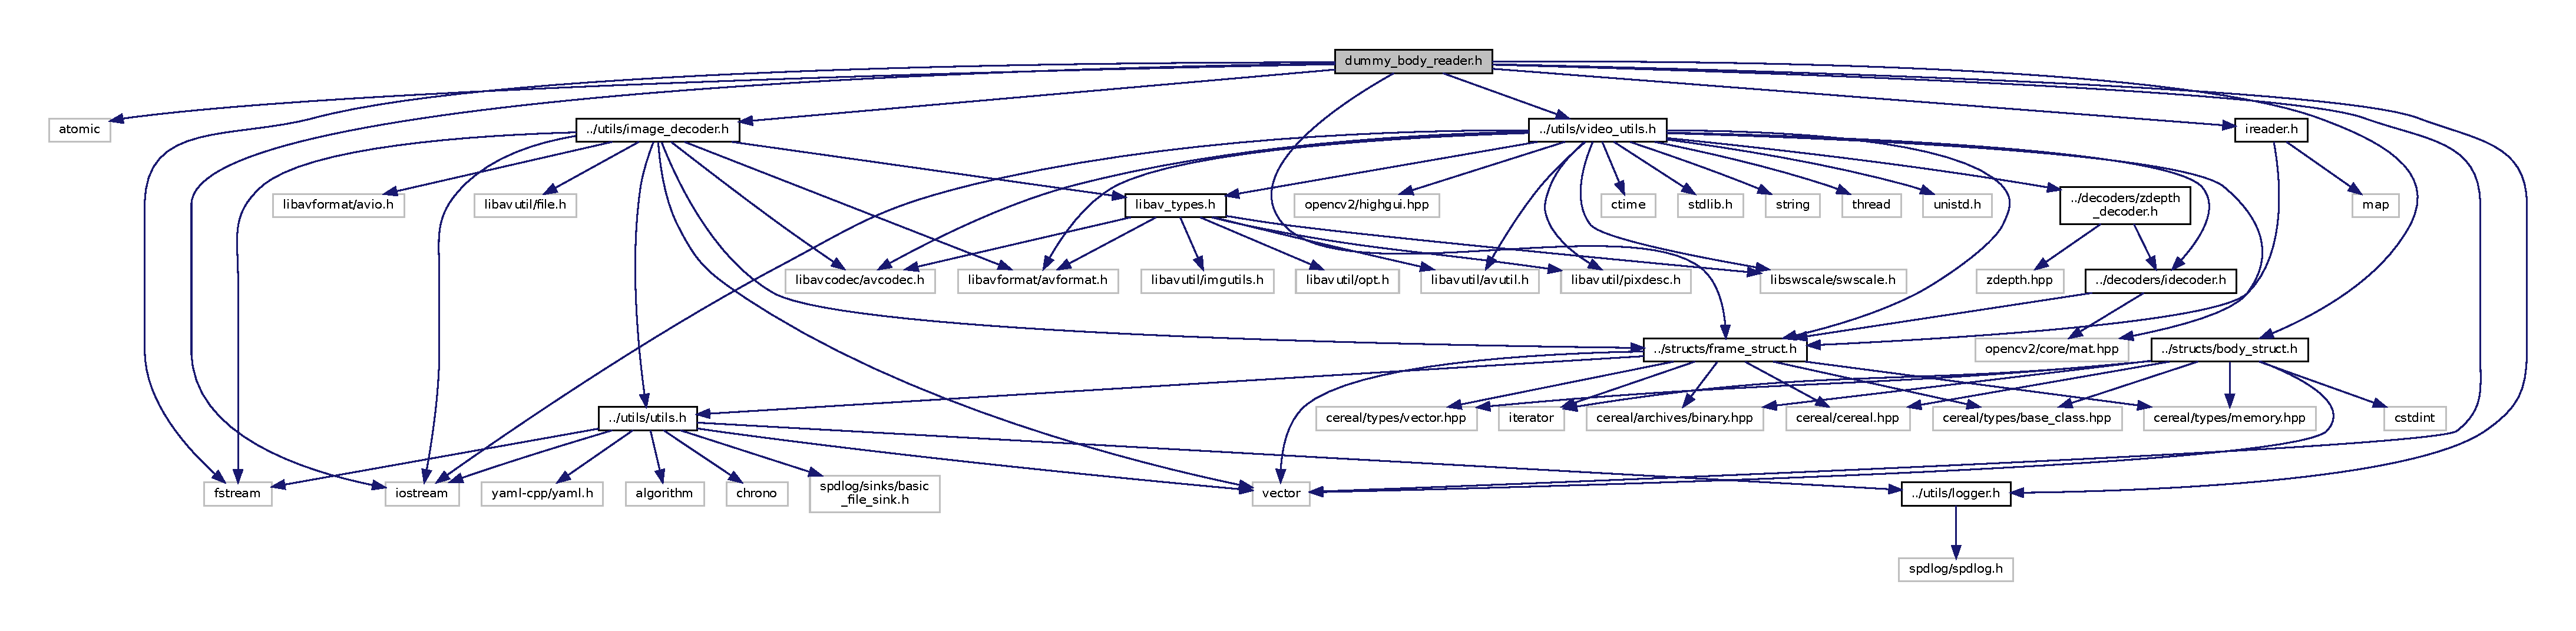
\includegraphics[width=350pt]{dummy__body__reader_8h__incl}
\end{center}
\end{figure}
This graph shows which files directly or indirectly include this file\+:
\nopagebreak
\begin{figure}[H]
\begin{center}
\leavevmode
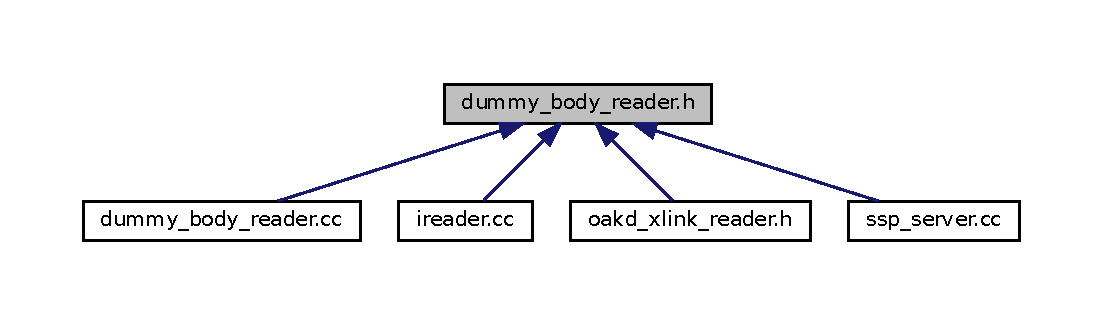
\includegraphics[width=350pt]{dummy__body__reader_8h__dep__incl}
\end{center}
\end{figure}
\subsection*{Classes}
\begin{DoxyCompactItemize}
\item 
class \hyperlink{classmoetsi_1_1ssp_1_1DummyBodyReader}{moetsi\+::ssp\+::\+Dummy\+Body\+Reader}
\end{DoxyCompactItemize}
\subsection*{Namespaces}
\begin{DoxyCompactItemize}
\item 
 \hyperlink{namespacemoetsi_1_1ssp}{moetsi\+::ssp}
\begin{DoxyCompactList}\small\item\em Sensor Stream Pipe. \end{DoxyCompactList}\end{DoxyCompactItemize}


\subsection{Detailed Description}
Dumy Body Reader. 


\hypertarget{idecoder_8cc}{}\doxysection{idecoder.\+cc File Reference}
\label{idecoder_8cc}\index{idecoder.cc@{idecoder.cc}}


I\+Decoder factory.  


{\ttfamily \#include \char`\"{}idecoder.\+h\char`\"{}}\newline
Include dependency graph for idecoder.\+cc\+:
% FIG 0
\doxysubsection*{Namespaces}
\begin{DoxyCompactItemize}
\item 
 \mbox{\hyperlink{namespacemoetsi}{moetsi}}
\begin{DoxyCompactList}\small\item\em Moetsi creations. \end{DoxyCompactList}\item 
 \mbox{\hyperlink{namespacemoetsi_1_1ssp}{moetsi\+::ssp}}
\begin{DoxyCompactList}\small\item\em Sensor Stream Pipe. \end{DoxyCompactList}\end{DoxyCompactItemize}
\doxysubsection*{Functions}
\begin{DoxyCompactItemize}
\item 
std\+::shared\+\_\+ptr$<$ I\+Decoder $>$ \mbox{\hyperlink{namespacemoetsi_1_1ssp_a9478a722eaeec487c7288ed18c9a06bc}{moetsi\+::ssp\+::\+I\+Decoder\+Factory}} (const std\+::string \&config)
\begin{DoxyCompactList}\small\item\em \mbox{\hyperlink{classmoetsi_1_1ssp_1_1IDecoder}{I\+Decoder}} factory. \end{DoxyCompactList}\end{DoxyCompactItemize}


\doxysubsection{Detailed Description}
I\+Decoder factory. 


\hypertarget{include_2decoders_2idecoder_8h}{}\section{idecoder.\+h File Reference}
\label{include_2decoders_2idecoder_8h}\index{idecoder.\+h@{idecoder.\+h}}


Frame decoder interface.  


{\ttfamily \#include \char`\"{}../structs/frame\+\_\+struct.\+h\char`\"{}}\newline
{\ttfamily \#include $<$opencv2/core/mat.\+hpp$>$}\newline
Include dependency graph for include/decoders/idecoder.h\+:
\nopagebreak
\begin{figure}[H]
\begin{center}
\leavevmode
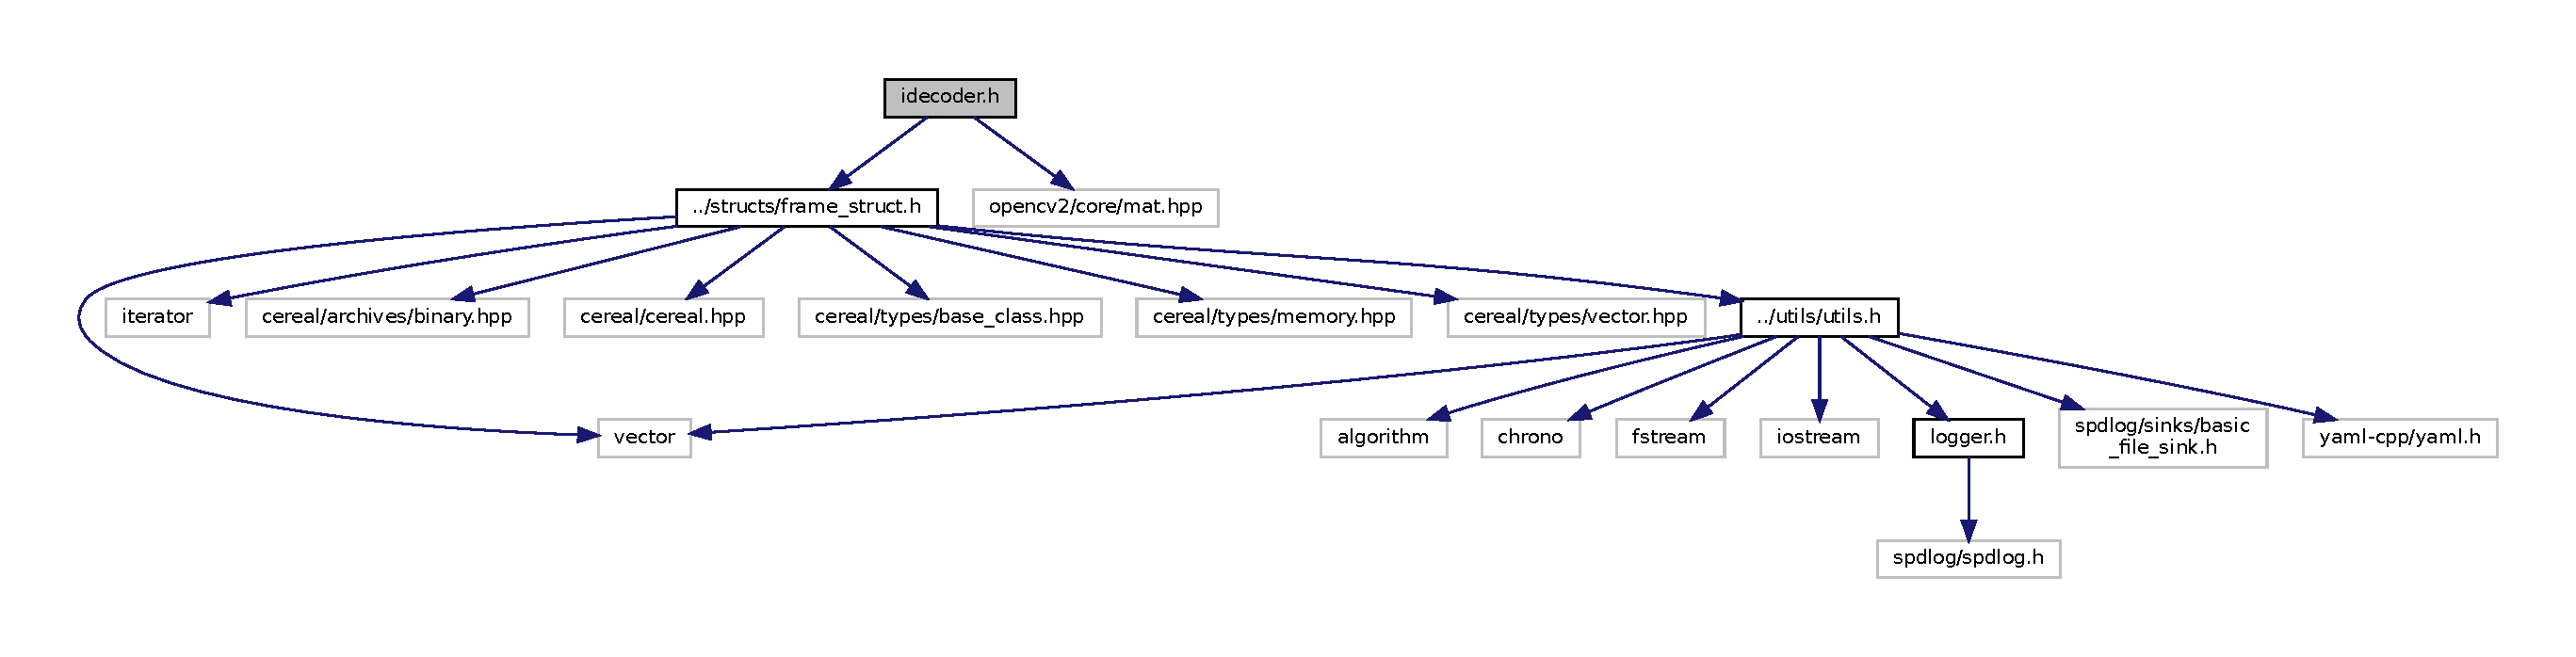
\includegraphics[width=350pt]{include_2decoders_2idecoder_8h__incl}
\end{center}
\end{figure}
This graph shows which files directly or indirectly include this file\+:
\nopagebreak
\begin{figure}[H]
\begin{center}
\leavevmode
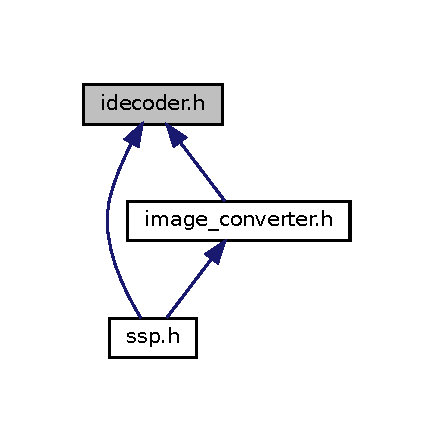
\includegraphics[width=199pt]{include_2decoders_2idecoder_8h__dep__incl}
\end{center}
\end{figure}
\subsection*{Classes}
\begin{DoxyCompactItemize}
\item 
class \hyperlink{classmoetsi_1_1ssp_1_1IDecoder}{moetsi\+::ssp\+::\+I\+Decoder}
\begin{DoxyCompactList}\small\item\em \hyperlink{classmoetsi_1_1ssp_1_1IDecoder}{I\+Decoder} abstract decoder interface. \end{DoxyCompactList}\end{DoxyCompactItemize}
\subsection*{Namespaces}
\begin{DoxyCompactItemize}
\item 
 \hyperlink{namespacemoetsi_1_1ssp}{moetsi\+::ssp}
\begin{DoxyCompactList}\small\item\em Sensor Stream Pipe. \end{DoxyCompactList}\end{DoxyCompactItemize}
\subsection*{Functions}
\begin{DoxyCompactItemize}
\item 
std\+::shared\+\_\+ptr$<$ I\+Decoder $>$ \hyperlink{namespacemoetsi_1_1ssp_a9478a722eaeec487c7288ed18c9a06bc}{moetsi\+::ssp\+::\+I\+Decoder\+Factory} (const std\+::string \&config)
\begin{DoxyCompactList}\small\item\em \hyperlink{classmoetsi_1_1ssp_1_1IDecoder}{I\+Decoder} factory. \end{DoxyCompactList}\end{DoxyCompactItemize}


\subsection{Detailed Description}
Frame decoder interface. 


\hypertarget{iencoder_8cc}{}\section{iencoder.\+cc File Reference}
\label{iencoder_8cc}\index{iencoder.\+cc@{iencoder.\+cc}}


I\+Encoder factory.  


{\ttfamily \#include \char`\"{}iencoder.\+h\char`\"{}}\newline
{\ttfamily \#include \char`\"{}../utils/logger.\+h\char`\"{}}\newline
{\ttfamily \#include $<$ctime$>$}\newline
{\ttfamily \#include $<$iostream$>$}\newline
{\ttfamily \#include $<$stdlib.\+h$>$}\newline
{\ttfamily \#include $<$string$>$}\newline
{\ttfamily \#include $<$thread$>$}\newline
{\ttfamily \#include $<$yaml-\/cpp/yaml.\+h$>$}\newline
{\ttfamily \#include $<$zmq.\+hpp$>$}\newline
{\ttfamily \#include \char`\"{}../encoders/libav\+\_\+encoder.\+h\char`\"{}}\newline
{\ttfamily \#include \char`\"{}../encoders/null\+\_\+encoder.\+h\char`\"{}}\newline
{\ttfamily \#include \char`\"{}../encoders/zdepth\+\_\+encoder.\+h\char`\"{}}\newline
{\ttfamily \#include \char`\"{}../readers/video\+\_\+file\+\_\+reader.\+h\char`\"{}}\newline
{\ttfamily \#include \char`\"{}../readers/multi\+\_\+image\+\_\+reader.\+h\char`\"{}}\newline
Include dependency graph for iencoder.\+cc\+:
\nopagebreak
\begin{figure}[H]
\begin{center}
\leavevmode
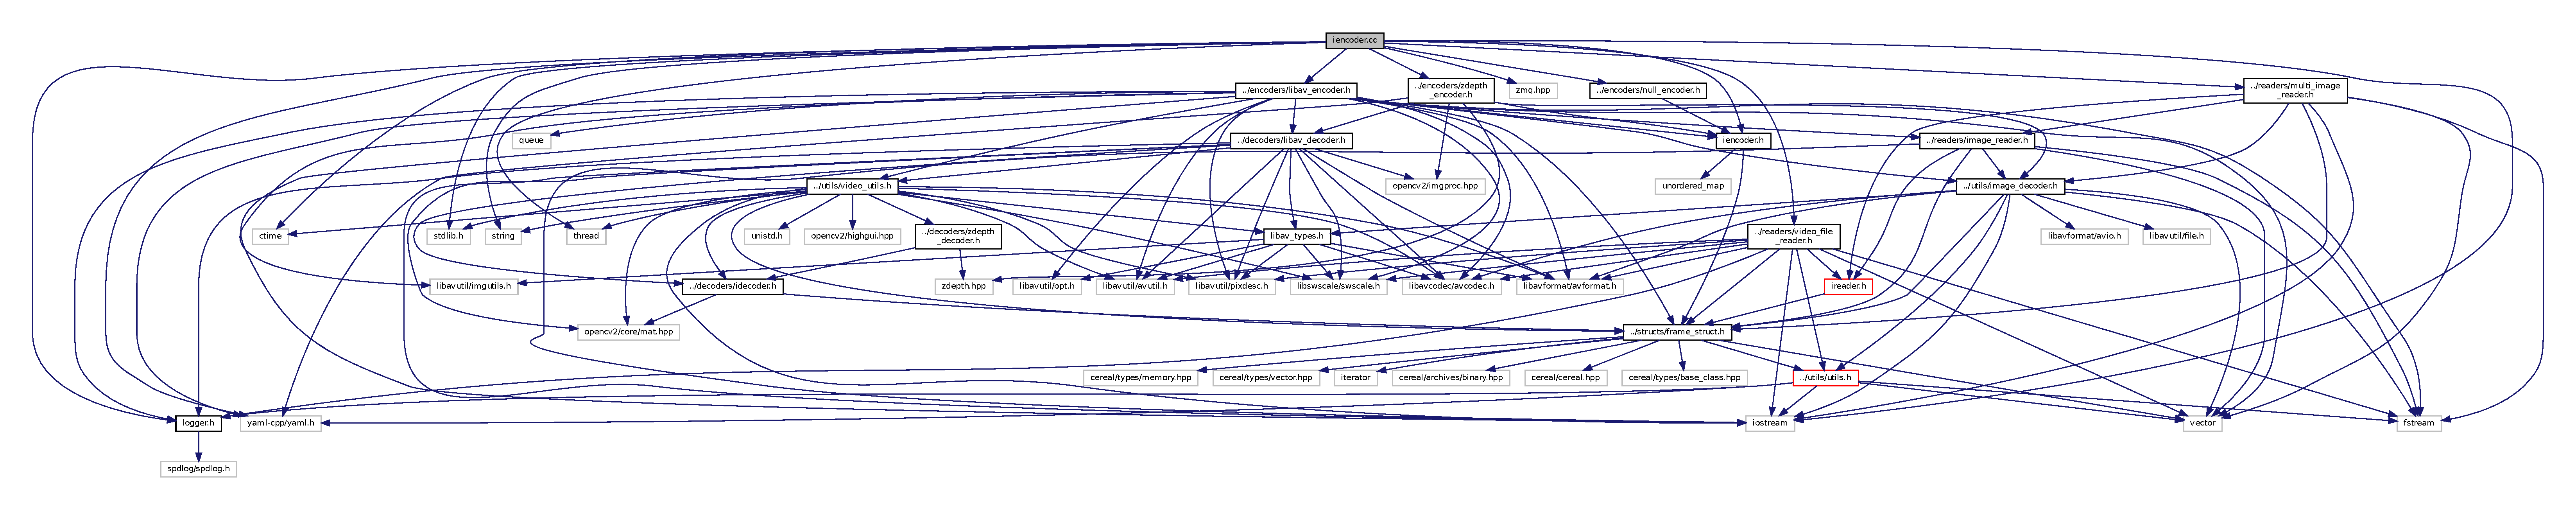
\includegraphics[width=350pt]{iencoder_8cc__incl}
\end{center}
\end{figure}
\subsection*{Namespaces}
\begin{DoxyCompactItemize}
\item 
 \hyperlink{namespacemoetsi_1_1ssp}{moetsi\+::ssp}
\begin{DoxyCompactList}\small\item\em Sensor Stream Pipe. \end{DoxyCompactList}\end{DoxyCompactItemize}
\subsection*{Functions}
\begin{DoxyCompactItemize}
\item 
std\+::unordered\+\_\+map$<$ Frame\+Type, std\+::shared\+\_\+ptr$<$ I\+Encoder $>$ $>$ \hyperlink{namespacemoetsi_1_1ssp_ad7a44286de625366acc78a320113e09b}{moetsi\+::ssp\+::\+I\+Encoder\+Factory} (const std\+::string \&config, const std\+::vector$<$ Frame\+Type $>$ \&types)
\begin{DoxyCompactList}\small\item\em \hyperlink{classmoetsi_1_1ssp_1_1IEncoder}{I\+Encoder} factory. \end{DoxyCompactList}\end{DoxyCompactItemize}


\subsection{Detailed Description}
I\+Encoder factory. 


\hypertarget{include_2encoders_2iencoder_8h}{}\doxysection{iencoder.\+h File Reference}
\label{include_2encoders_2iencoder_8h}\index{iencoder.h@{iencoder.h}}


I\+Encoder factory.  


{\ttfamily \#include \char`\"{}../structs/frame\+\_\+struct.\+h\char`\"{}}\newline
{\ttfamily \#include $<$unordered\+\_\+map$>$}\newline
Include dependency graph for include/encoders/iencoder.h\+:
% FIG 0
This graph shows which files directly or indirectly include this file\+:
% FIG 1
\doxysubsection*{Classes}
\begin{DoxyCompactItemize}
\item 
class \mbox{\hyperlink{classmoetsi_1_1ssp_1_1IEncoder}{moetsi\+::ssp\+::\+I\+Encoder}}
\begin{DoxyCompactList}\small\item\em \mbox{\hyperlink{classmoetsi_1_1ssp_1_1IEncoder}{I\+Encoder}} abstract encoder class. \end{DoxyCompactList}\end{DoxyCompactItemize}
\doxysubsection*{Namespaces}
\begin{DoxyCompactItemize}
\item 
 \mbox{\hyperlink{namespacemoetsi}{moetsi}}
\begin{DoxyCompactList}\small\item\em Moetsi creations. \end{DoxyCompactList}\item 
 \mbox{\hyperlink{namespacemoetsi_1_1ssp}{moetsi\+::ssp}}
\begin{DoxyCompactList}\small\item\em Sensor Stream Pipe. \end{DoxyCompactList}\end{DoxyCompactItemize}
\doxysubsection*{Functions}
\begin{DoxyCompactItemize}
\item 
std\+::unordered\+\_\+map$<$ Frame\+Type, std\+::shared\+\_\+ptr$<$ I\+Encoder $>$ $>$ \mbox{\hyperlink{namespacemoetsi_1_1ssp_ad7a44286de625366acc78a320113e09b}{moetsi\+::ssp\+::\+I\+Encoder\+Factory}} (const std\+::string \&config, const std\+::vector$<$ Frame\+Type $>$ \&types)
\begin{DoxyCompactList}\small\item\em \mbox{\hyperlink{classmoetsi_1_1ssp_1_1IEncoder}{I\+Encoder}} factory. \end{DoxyCompactList}\end{DoxyCompactItemize}


\doxysubsection{Detailed Description}
I\+Encoder factory. 

I\+Encoder definition\+: frame encoder.
\hypertarget{image__converter_8cc}{}\section{image\+\_\+converter.\+cc File Reference}
\label{image__converter_8cc}\index{image\+\_\+converter.\+cc@{image\+\_\+converter.\+cc}}


Image converter from frame struct to opencv image.  


{\ttfamily \#include \char`\"{}image\+\_\+converter.\+h\char`\"{}}\newline
{\ttfamily \#include \char`\"{}../decoders/libav\+\_\+decoder.\+h\char`\"{}}\newline
{\ttfamily \#include \char`\"{}../decoders/zdepth\+\_\+decoder.\+h\char`\"{}}\newline
Include dependency graph for image\+\_\+converter.\+cc\+:
\nopagebreak
\begin{figure}[H]
\begin{center}
\leavevmode
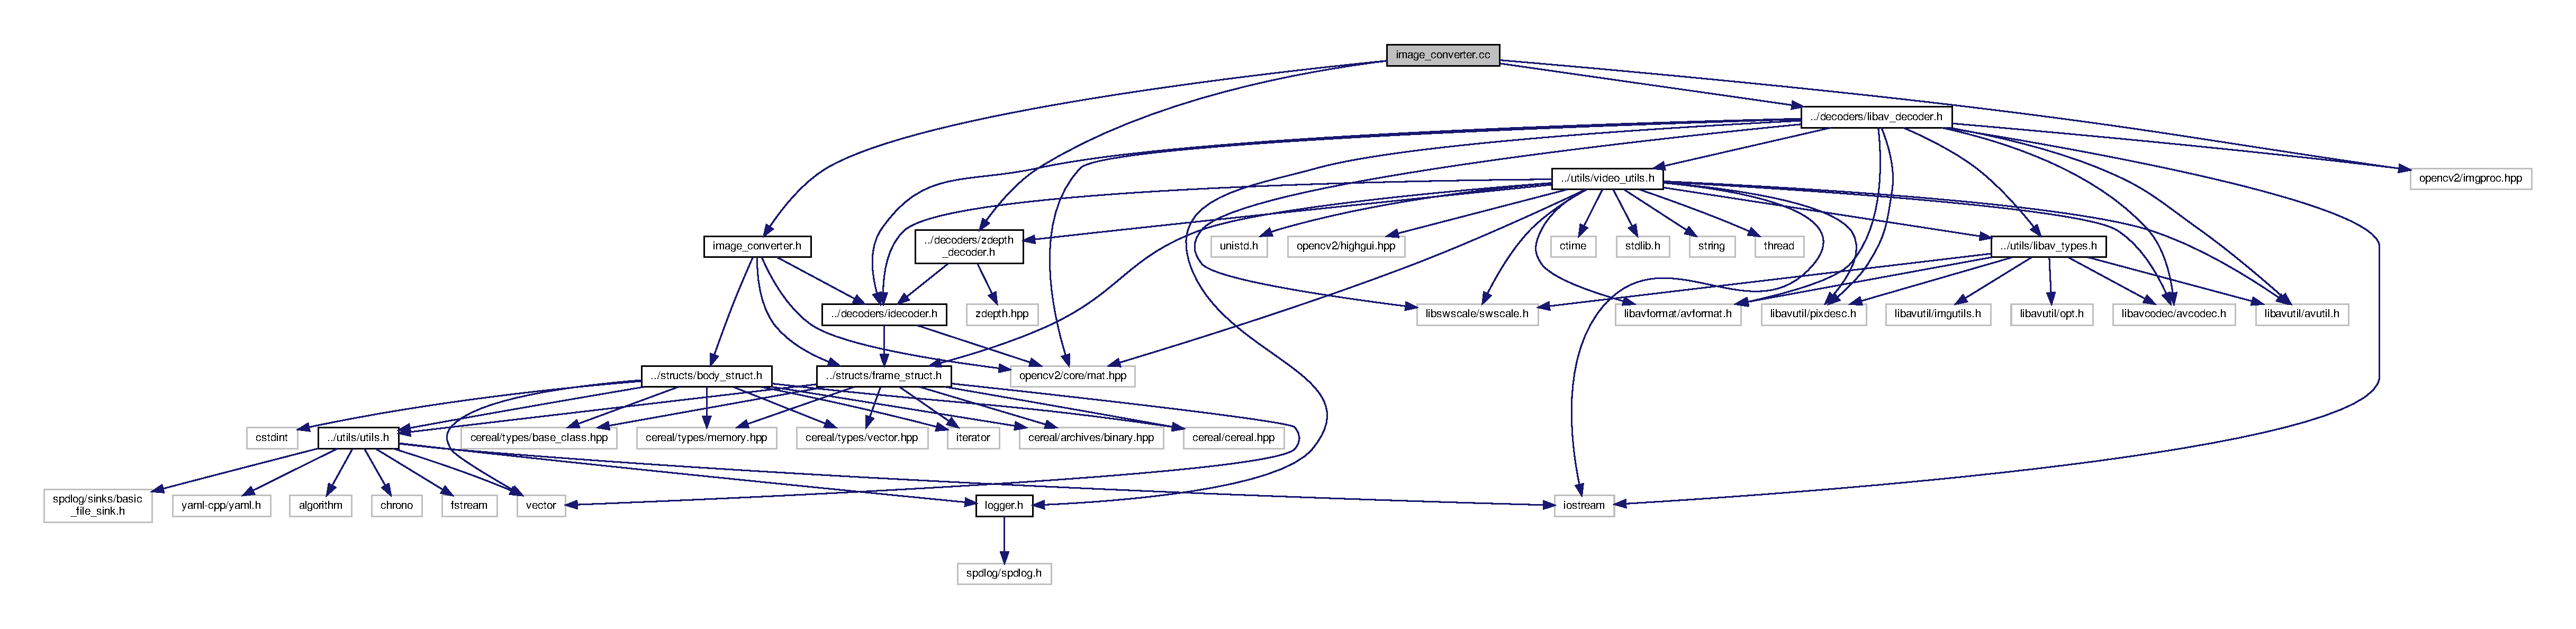
\includegraphics[width=350pt]{image__converter_8cc__incl}
\end{center}
\end{figure}
\subsection*{Namespaces}
\begin{DoxyCompactItemize}
\item 
 \hyperlink{namespacemoetsi_1_1ssp}{moetsi\+::ssp}
\begin{DoxyCompactList}\small\item\em Sensor Stream Pipe. \end{DoxyCompactList}\end{DoxyCompactItemize}
\subsection*{Functions}
\begin{DoxyCompactItemize}
\item 
bool \hyperlink{namespacemoetsi_1_1ssp_ac87377cef5da79f1a9cf7a4acdc42af6}{moetsi\+::ssp\+::\+Frame\+Struct\+To\+Mat} (\hyperlink{structFrameStruct}{Frame\+Struct} \&f, cv\+::\+Mat \&img, std\+::unordered\+\_\+map$<$ std\+::string, std\+::shared\+\_\+ptr$<$ I\+Decoder $>$$>$ \&decoders)
\begin{DoxyCompactList}\small\item\em Convert frame struct to opencv matrix. \end{DoxyCompactList}\end{DoxyCompactItemize}


\subsection{Detailed Description}
Image converter from frame struct to opencv image. 


\hypertarget{image__decoder_8cc}{}\doxysection{image\+\_\+decoder.\+cc File Reference}
\label{image__decoder_8cc}\index{image\_decoder.cc@{image\_decoder.cc}}


mpeg/jpeg image decoder  


{\ttfamily \#include \char`\"{}image\+\_\+decoder.\+h\char`\"{}}\newline
Include dependency graph for image\+\_\+decoder.\+cc\+:
\nopagebreak
\begin{figure}[H]
\begin{center}
\leavevmode
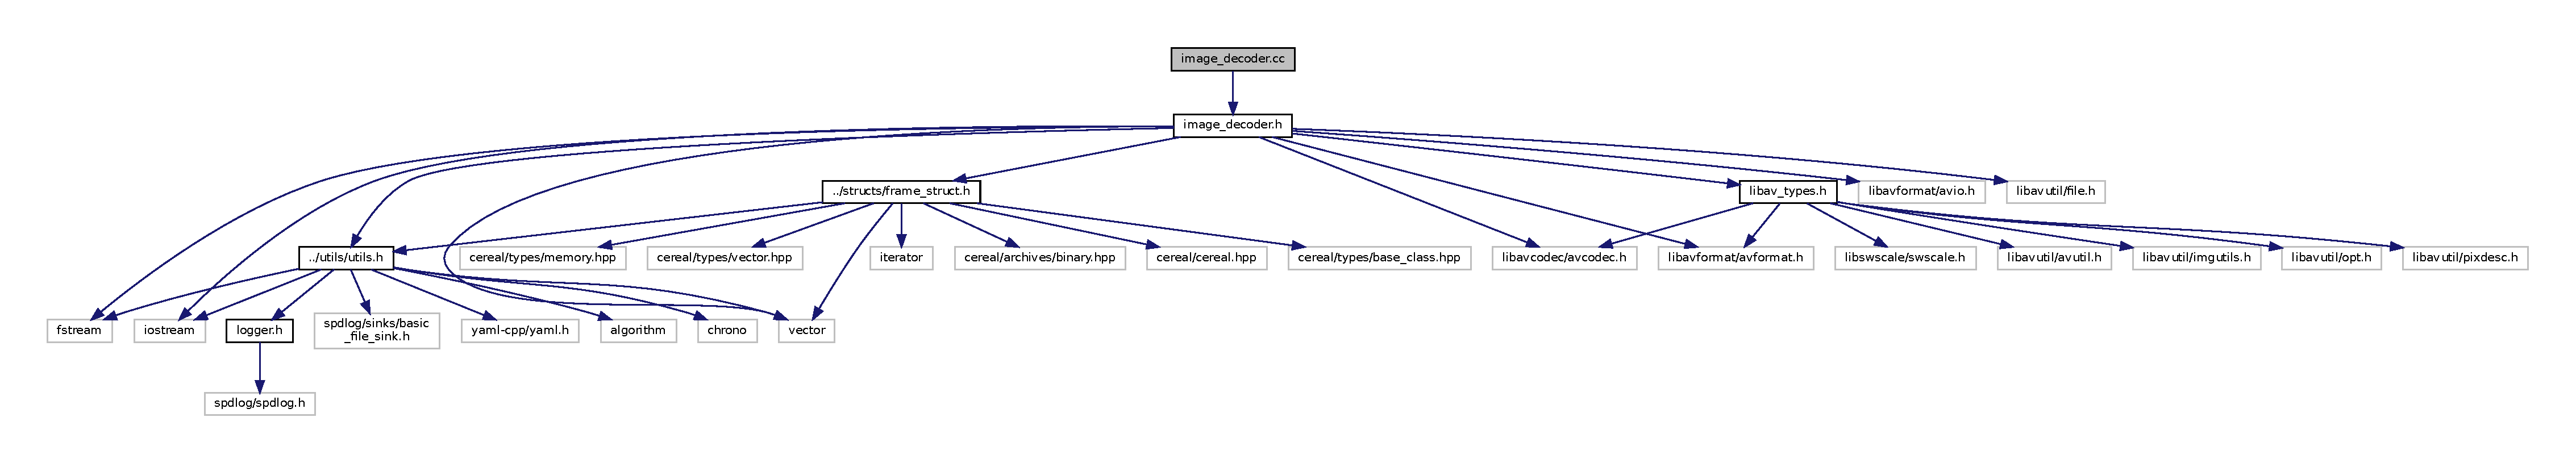
\includegraphics[width=350pt]{image__decoder_8cc__incl}
\end{center}
\end{figure}
\doxysubsection*{Classes}
\begin{DoxyCompactItemize}
\item 
struct \mbox{\hyperlink{structmoetsi_1_1ssp_1_1buffer__data}{moetsi\+::ssp\+::buffer\+\_\+data}}
\end{DoxyCompactItemize}
\doxysubsection*{Namespaces}
\begin{DoxyCompactItemize}
\item 
 \mbox{\hyperlink{namespacemoetsi}{moetsi}}
\begin{DoxyCompactList}\small\item\em Moetsi creations. \end{DoxyCompactList}\item 
 \mbox{\hyperlink{namespacemoetsi_1_1ssp}{moetsi\+::ssp}}
\begin{DoxyCompactList}\small\item\em Sensor Stream Pipe. \end{DoxyCompactList}\end{DoxyCompactItemize}


\doxysubsection{Detailed Description}
mpeg/jpeg image decoder 


\hypertarget{image__decoder_8h}{}\doxysection{image\+\_\+decoder.\+h File Reference}
\label{image__decoder_8h}\index{image\_decoder.h@{image\_decoder.h}}


AV Image decoder.  


{\ttfamily \#include $<$fstream$>$}\newline
{\ttfamily \#include $<$iostream$>$}\newline
{\ttfamily \#include $<$vector$>$}\newline
{\ttfamily \#include $<$libavcodec/avcodec.\+h$>$}\newline
{\ttfamily \#include $<$libavformat/avformat.\+h$>$}\newline
{\ttfamily \#include $<$libavformat/avio.\+h$>$}\newline
{\ttfamily \#include $<$libavutil/file.\+h$>$}\newline
{\ttfamily \#include \char`\"{}../structs/frame\+\_\+struct.\+h\char`\"{}}\newline
{\ttfamily \#include \char`\"{}libav\+\_\+types.\+h\char`\"{}}\newline
{\ttfamily \#include \char`\"{}utils.\+h\char`\"{}}\newline
Include dependency graph for image\+\_\+decoder.\+h\+:
% FIG 0
This graph shows which files directly or indirectly include this file\+:
% FIG 1
\doxysubsection*{Classes}
\begin{DoxyCompactItemize}
\item 
class \mbox{\hyperlink{classmoetsi_1_1ssp_1_1ImageDecoder}{moetsi\+::ssp\+::\+Image\+Decoder}}
\begin{DoxyCompactList}\small\item\em Decode image to AV frame. \end{DoxyCompactList}\end{DoxyCompactItemize}
\doxysubsection*{Namespaces}
\begin{DoxyCompactItemize}
\item 
 \mbox{\hyperlink{namespacemoetsi}{moetsi}}
\begin{DoxyCompactList}\small\item\em Moetsi creations. \end{DoxyCompactList}\item 
 \mbox{\hyperlink{namespacemoetsi_1_1ssp}{moetsi\+::ssp}}
\begin{DoxyCompactList}\small\item\em Sensor Stream Pipe. \end{DoxyCompactList}\end{DoxyCompactItemize}


\doxysubsection{Detailed Description}
AV Image decoder. 


\hypertarget{image__reader_8cc}{}\doxysection{image\+\_\+reader.\+cc File Reference}
\label{image__reader_8cc}\index{image\_reader.cc@{image\_reader.cc}}


Image reader.  


{\ttfamily \#include \char`\"{}image\+\_\+reader.\+h\char`\"{}}\newline
Include dependency graph for image\+\_\+reader.\+cc\+:
\nopagebreak
\begin{figure}[H]
\begin{center}
\leavevmode
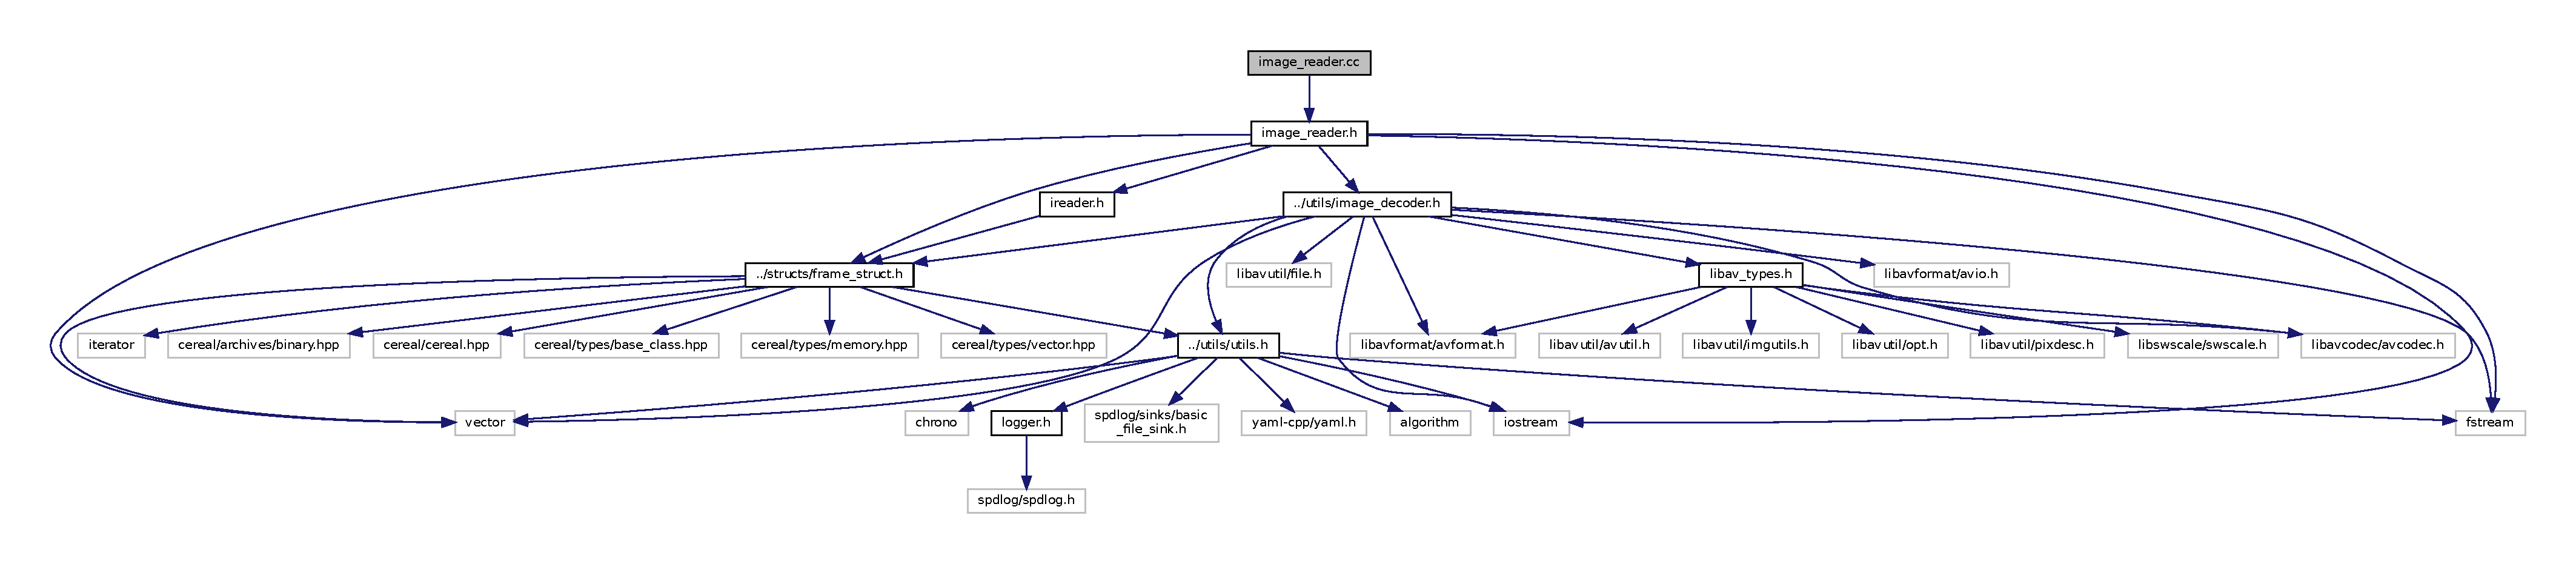
\includegraphics[width=350pt]{image__reader_8cc__incl}
\end{center}
\end{figure}
\doxysubsection*{Namespaces}
\begin{DoxyCompactItemize}
\item 
 \mbox{\hyperlink{namespacemoetsi}{moetsi}}
\begin{DoxyCompactList}\small\item\em Moetsi creations. \end{DoxyCompactList}\item 
 \mbox{\hyperlink{namespacemoetsi_1_1ssp}{moetsi\+::ssp}}
\begin{DoxyCompactList}\small\item\em Sensor Stream Pipe. \end{DoxyCompactList}\end{DoxyCompactItemize}


\doxysubsection{Detailed Description}
Image reader. 


\hypertarget{image__reader_8h}{}\doxysection{image\+\_\+reader.\+h File Reference}
\label{image__reader_8h}\index{image\_reader.h@{image\_reader.h}}


Image reader.  


{\ttfamily \#include $<$fstream$>$}\newline
{\ttfamily \#include $<$iostream$>$}\newline
{\ttfamily \#include $<$vector$>$}\newline
{\ttfamily \#include \char`\"{}../structs/frame\+\_\+struct.\+h\char`\"{}}\newline
{\ttfamily \#include \char`\"{}../utils/image\+\_\+decoder.\+h\char`\"{}}\newline
{\ttfamily \#include \char`\"{}ireader.\+h\char`\"{}}\newline
Include dependency graph for image\+\_\+reader.\+h\+:
% FIG 0
This graph shows which files directly or indirectly include this file\+:
% FIG 1
\doxysubsection*{Classes}
\begin{DoxyCompactItemize}
\item 
class \mbox{\hyperlink{classmoetsi_1_1ssp_1_1ImageReader}{moetsi\+::ssp\+::\+Image\+Reader}}
\end{DoxyCompactItemize}
\doxysubsection*{Namespaces}
\begin{DoxyCompactItemize}
\item 
 \mbox{\hyperlink{namespacemoetsi}{moetsi}}
\begin{DoxyCompactList}\small\item\em Moetsi creations. \end{DoxyCompactList}\item 
 \mbox{\hyperlink{namespacemoetsi_1_1ssp}{moetsi\+::ssp}}
\begin{DoxyCompactList}\small\item\em Sensor Stream Pipe. \end{DoxyCompactList}\end{DoxyCompactItemize}


\doxysubsection{Detailed Description}
Image reader. 


\hypertarget{iphone__reader_8h}{}\doxysection{iphone\+\_\+reader.\+h File Reference}
\label{iphone__reader_8h}\index{iphone\_reader.h@{iphone\_reader.h}}


i\+Phone driver  


{\ttfamily \#include $<$vector$>$}\newline
{\ttfamily \#include \char`\"{}../structs/frame\+\_\+struct.\+h\char`\"{}}\newline
{\ttfamily \#include \char`\"{}ireader.\+h\char`\"{}}\newline
Include dependency graph for iphone\+\_\+reader.\+h\+:
\nopagebreak
\begin{figure}[H]
\begin{center}
\leavevmode
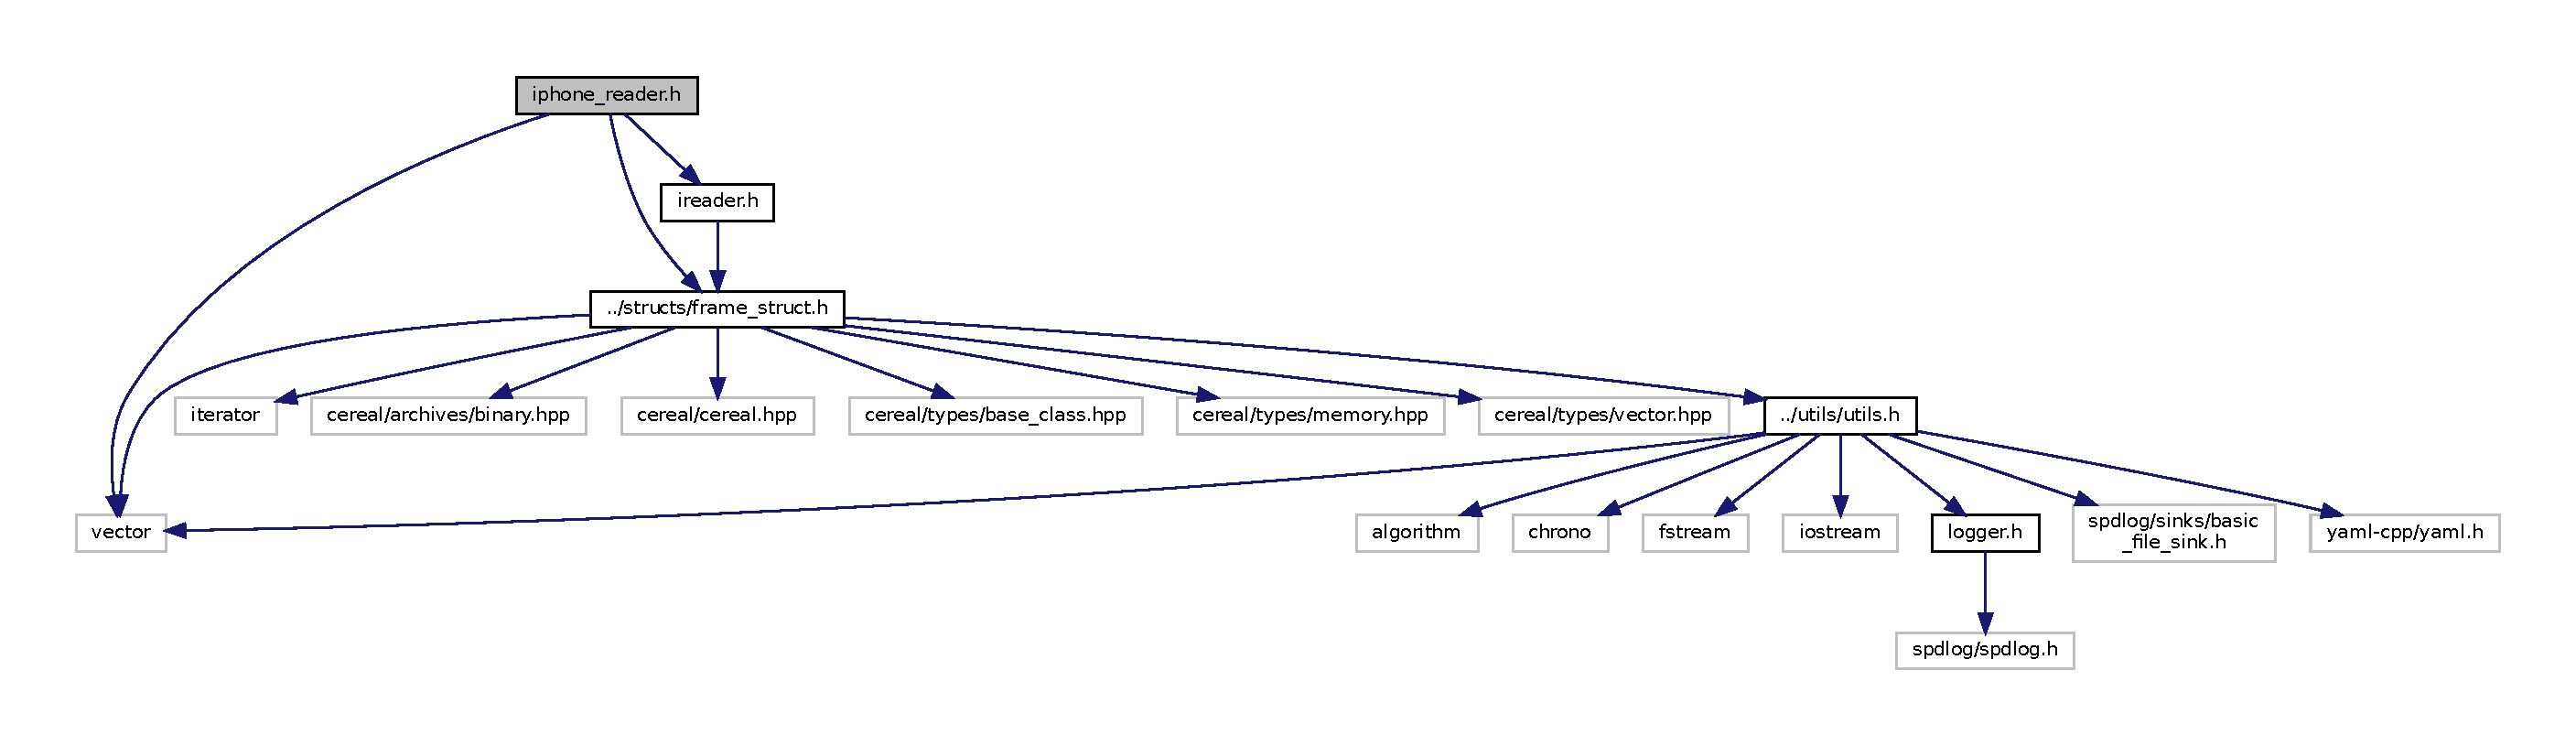
\includegraphics[width=350pt]{iphone__reader_8h__incl}
\end{center}
\end{figure}
This graph shows which files directly or indirectly include this file\+:
\nopagebreak
\begin{figure}[H]
\begin{center}
\leavevmode
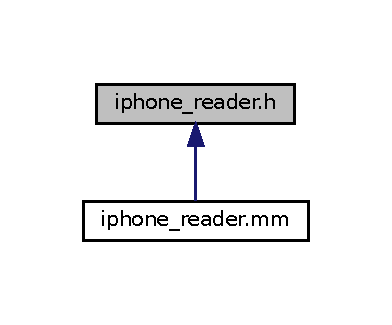
\includegraphics[width=188pt]{iphone__reader_8h__dep__incl}
\end{center}
\end{figure}
\doxysubsection*{Classes}
\begin{DoxyCompactItemize}
\item 
class \mbox{\hyperlink{classmoetsi_1_1ssp_1_1iPhoneReader}{moetsi\+::ssp\+::i\+Phone\+Reader}}
\end{DoxyCompactItemize}
\doxysubsection*{Namespaces}
\begin{DoxyCompactItemize}
\item 
 \mbox{\hyperlink{namespacemoetsi}{moetsi}}
\begin{DoxyCompactList}\small\item\em Moetsi creations. \end{DoxyCompactList}\item 
 \mbox{\hyperlink{namespacemoetsi_1_1ssp}{moetsi\+::ssp}}
\begin{DoxyCompactList}\small\item\em Sensor Stream Pipe. \end{DoxyCompactList}\end{DoxyCompactItemize}


\doxysubsection{Detailed Description}
i\+Phone driver 


\hypertarget{iphone__reader_8mm}{}\doxysection{iphone\+\_\+reader.\+mm File Reference}
\label{iphone__reader_8mm}\index{iphone\_reader.mm@{iphone\_reader.mm}}


i\+Phone driver  


{\ttfamily \#include \char`\"{}iphone\+\_\+reader.\+h\char`\"{}}\newline
{\ttfamily \#include $<$opencv2/imgproc.\+hpp$>$}\newline
{\ttfamily \#import $<$A\+R\+Kit/\+A\+R\+Kit.\+h$>$}\newline
{\ttfamily \#include $<$mach/mach\+\_\+init.\+h$>$}\newline
{\ttfamily \#include $<$mach/mach\+\_\+error.\+h$>$}\newline
{\ttfamily \#include $<$mach/semaphore.\+h$>$}\newline
{\ttfamily \#include $<$mach/task.\+h$>$}\newline
Include dependency graph for iphone\+\_\+reader.\+mm\+:
\nopagebreak
\begin{figure}[H]
\begin{center}
\leavevmode
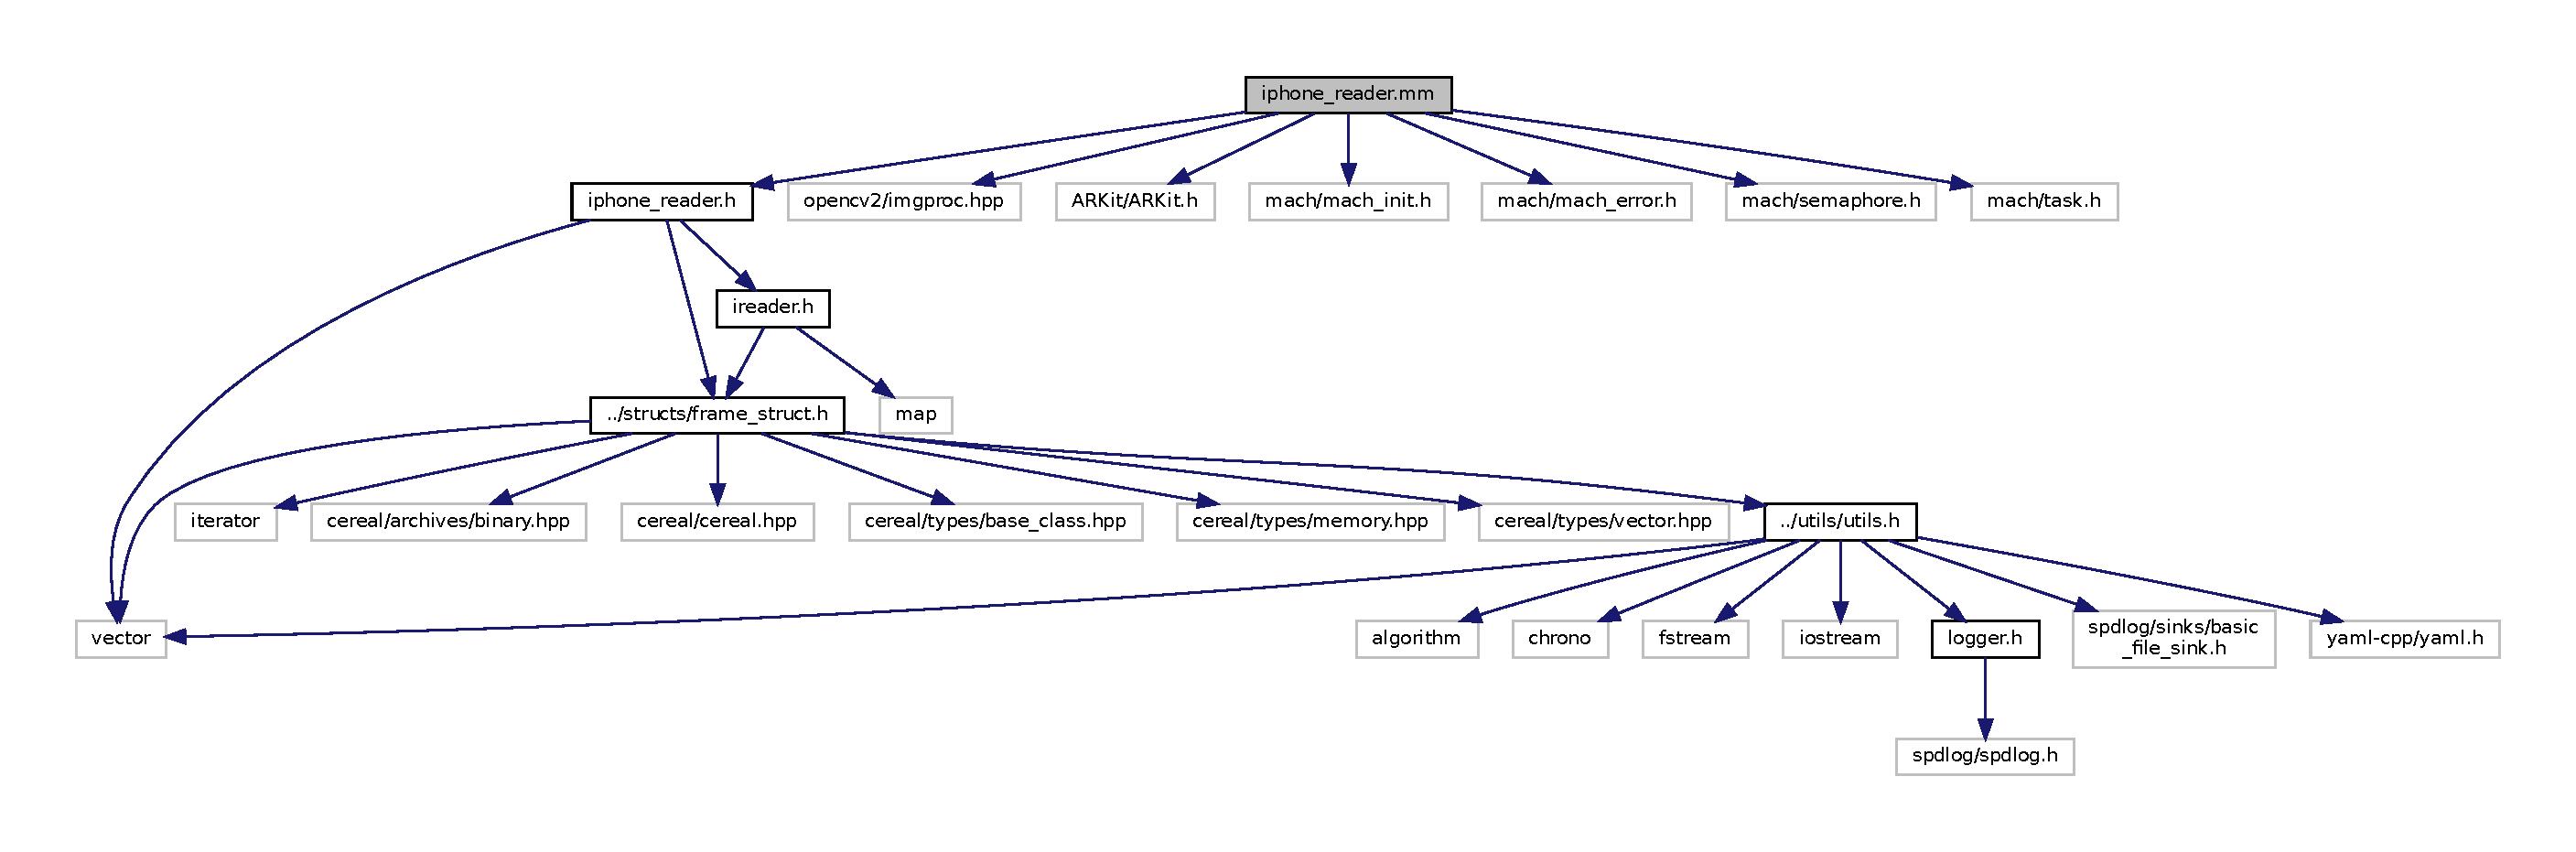
\includegraphics[width=350pt]{iphone__reader_8mm__incl}
\end{center}
\end{figure}
\doxysubsection*{Classes}
\begin{DoxyCompactItemize}
\item 
class \mbox{\hyperlink{interfaceSessionDelegate}{Session\+Delegate}}
\item 
struct \mbox{\hyperlink{structUnityXRNativeSessionPtr}{Unity\+X\+R\+Native\+Session\+Ptr}}
\item 
class \mbox{\hyperlink{classmoetsi_1_1ssp_1_1iPhoneReaderImpl}{moetsi\+::ssp\+::i\+Phone\+Reader\+Impl}}
\end{DoxyCompactItemize}
\doxysubsection*{Namespaces}
\begin{DoxyCompactItemize}
\item 
 \mbox{\hyperlink{namespacemoetsi}{moetsi}}
\begin{DoxyCompactList}\small\item\em Moetsi creations. \end{DoxyCompactList}\item 
 \mbox{\hyperlink{namespacemoetsi_1_1ssp}{moetsi\+::ssp}}
\begin{DoxyCompactList}\small\item\em Sensor Stream Pipe. \end{DoxyCompactList}\end{DoxyCompactItemize}
\doxysubsection*{Functions}
\begin{DoxyCompactItemize}
\item 
\mbox{\Hypertarget{iphone__reader_8mm_aea1fc7a3a8cfe6ce9c958525ff814fba}\label{iphone__reader_8mm_aea1fc7a3a8cfe6ce9c958525ff814fba}} 
void {\bfseries use\+\_\+session} (void $\ast$session)
\end{DoxyCompactItemize}


\doxysubsection{Detailed Description}
i\+Phone driver 


\hypertarget{ireader_8cc}{}\doxysection{ireader.\+cc File Reference}
\label{ireader_8cc}\index{ireader.cc@{ireader.cc}}


I\+Reader factory.  


{\ttfamily \#include \char`\"{}ireader.\+h\char`\"{}}\newline
{\ttfamily \#include \char`\"{}../utils/logger.\+h\char`\"{}}\newline
{\ttfamily \#include $<$ctime$>$}\newline
{\ttfamily \#include $<$iostream$>$}\newline
{\ttfamily \#include $<$stdlib.\+h$>$}\newline
{\ttfamily \#include $<$string$>$}\newline
{\ttfamily \#include $<$thread$>$}\newline
{\ttfamily \#include $<$yaml-\/cpp/yaml.\+h$>$}\newline
{\ttfamily \#include $<$zmq.\+hpp$>$}\newline
{\ttfamily \#include \char`\"{}../encoders/libav\+\_\+encoder.\+h\char`\"{}}\newline
{\ttfamily \#include \char`\"{}../encoders/null\+\_\+encoder.\+h\char`\"{}}\newline
{\ttfamily \#include \char`\"{}../encoders/zdepth\+\_\+encoder.\+h\char`\"{}}\newline
{\ttfamily \#include \char`\"{}../readers/video\+\_\+file\+\_\+reader.\+h\char`\"{}}\newline
{\ttfamily \#include \char`\"{}../readers/multi\+\_\+image\+\_\+reader.\+h\char`\"{}}\newline
{\ttfamily \#include \char`\"{}../readers/dummy\+\_\+body\+\_\+reader.\+h\char`\"{}}\newline
Include dependency graph for ireader.\+cc\+:
\nopagebreak
\begin{figure}[H]
\begin{center}
\leavevmode
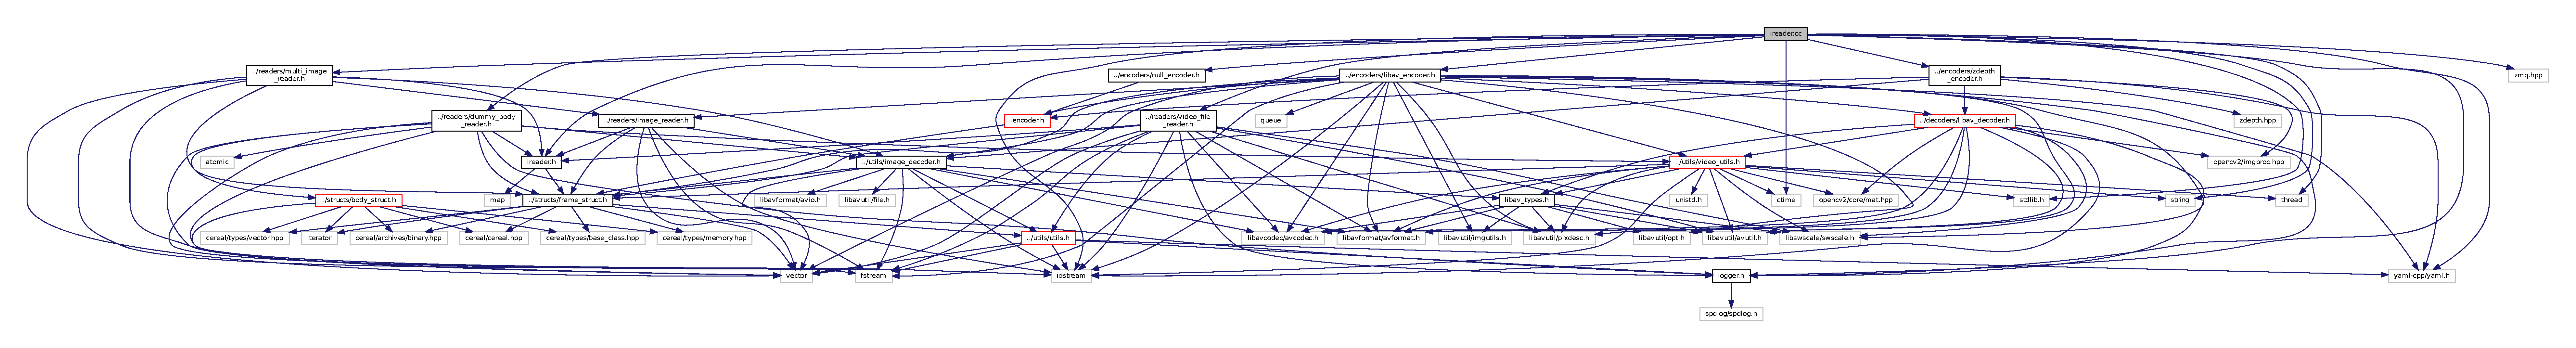
\includegraphics[width=350pt]{ireader_8cc__incl}
\end{center}
\end{figure}
\doxysubsection*{Namespaces}
\begin{DoxyCompactItemize}
\item 
 \mbox{\hyperlink{namespacemoetsi}{moetsi}}
\begin{DoxyCompactList}\small\item\em Moetsi creations. \end{DoxyCompactList}\item 
 \mbox{\hyperlink{namespacemoetsi_1_1ssp}{moetsi\+::ssp}}
\begin{DoxyCompactList}\small\item\em Sensor Stream Pipe. \end{DoxyCompactList}\end{DoxyCompactItemize}
\doxysubsection*{Functions}
\begin{DoxyCompactItemize}
\item 
std\+::string \mbox{\hyperlink{namespacemoetsi_1_1ssp_abe74cbb741dec4bebb18148c17158e7d}{moetsi\+::ssp\+::\+String\+Interpolation}} (const std\+::map$<$ std\+::string, std\+::string $>$ \&env, const std\+::string \&s)
\begin{DoxyCompactList}\small\item\em Magic string interpolation. \end{DoxyCompactList}\item 
std\+::string \mbox{\hyperlink{namespacemoetsi_1_1ssp_a6454f35414e723f6f49c182bb511c02c}{moetsi\+::ssp\+::\+String\+Interpolation}} (const std\+::string \&s)
\begin{DoxyCompactList}\small\item\em Magic string interpolation. \end{DoxyCompactList}\item 
std\+::shared\+\_\+ptr$<$ I\+Reader $>$ \mbox{\hyperlink{namespacemoetsi_1_1ssp_ad5e820c4c6a1a43d5e85608a06b86ea8}{moetsi\+::ssp\+::\+I\+Reader\+Factory}} (const std\+::string \&config)
\begin{DoxyCompactList}\small\item\em \mbox{\hyperlink{classmoetsi_1_1ssp_1_1IReader}{I\+Reader}} factory. \end{DoxyCompactList}\end{DoxyCompactItemize}


\doxysubsection{Detailed Description}
I\+Reader factory. 


\hypertarget{kinect__reader_8cc}{}\section{kinect\+\_\+reader.\+cc File Reference}
\label{kinect__reader_8cc}\index{kinect\+\_\+reader.\+cc@{kinect\+\_\+reader.\+cc}}


Kinect driver.  


{\ttfamily \#include \char`\"{}kinect\+\_\+reader.\+h\char`\"{}}\newline
Include dependency graph for kinect\+\_\+reader.\+cc\+:
\nopagebreak
\begin{figure}[H]
\begin{center}
\leavevmode
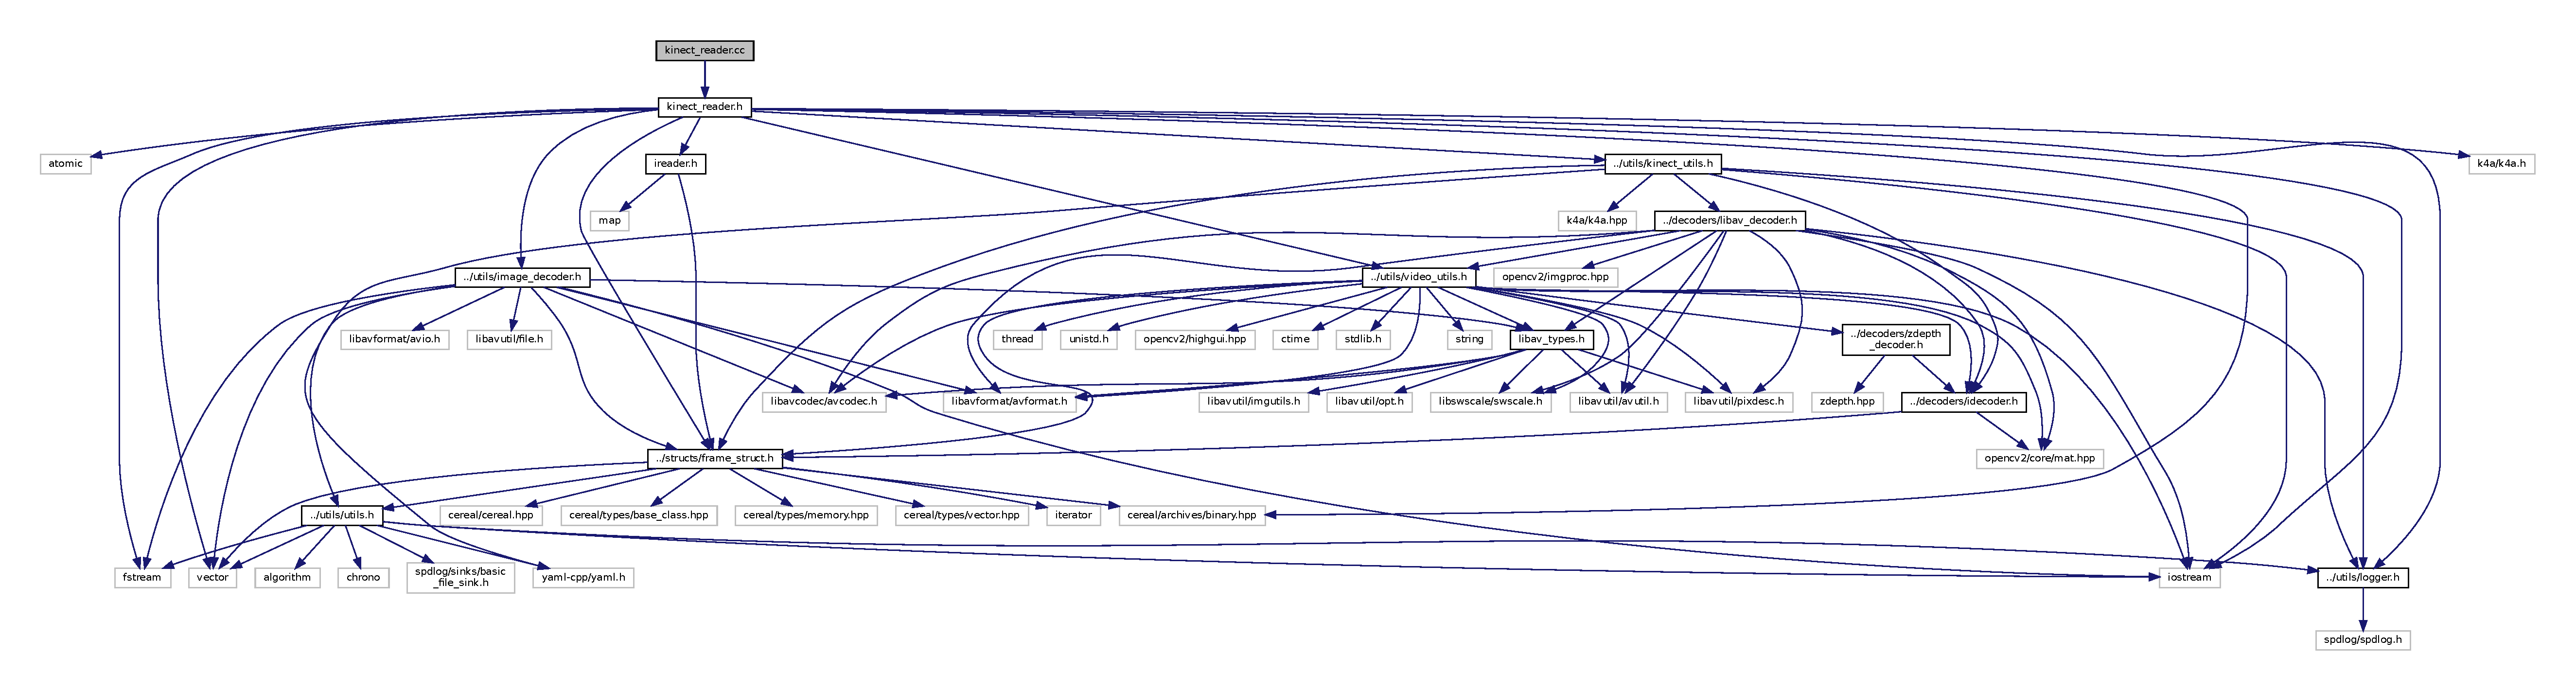
\includegraphics[width=350pt]{kinect__reader_8cc__incl}
\end{center}
\end{figure}
\subsection*{Namespaces}
\begin{DoxyCompactItemize}
\item 
 \hyperlink{namespacemoetsi_1_1ssp}{moetsi\+::ssp}
\begin{DoxyCompactList}\small\item\em Sensor Stream Pipe. \end{DoxyCompactList}\end{DoxyCompactItemize}
\subsection*{Functions}
\begin{DoxyCompactItemize}
\item 
\mbox{\Hypertarget{namespacemoetsi_1_1ssp_a316383e8c51e6cb5f67a013bd0311bb8}\label{namespacemoetsi_1_1ssp_a316383e8c51e6cb5f67a013bd0311bb8}} 
std\+::atomic\+\_\+bool {\bfseries moetsi\+::ssp\+::exiting} (false)
\end{DoxyCompactItemize}


\subsection{Detailed Description}
Kinect driver. 


\hypertarget{kinect__reader_8h}{}\doxysection{kinect\+\_\+reader.\+h File Reference}
\label{kinect__reader_8h}\index{kinect\_reader.h@{kinect\_reader.h}}


Kinect driver.  


{\ttfamily \#include $<$atomic$>$}\newline
{\ttfamily \#include $<$fstream$>$}\newline
{\ttfamily \#include $<$iostream$>$}\newline
{\ttfamily \#include $<$vector$>$}\newline
{\ttfamily \#include \char`\"{}../utils/logger.\+h\char`\"{}}\newline
{\ttfamily \#include $<$k4a/k4a.\+h$>$}\newline
{\ttfamily \#include $<$cereal/archives/binary.\+hpp$>$}\newline
{\ttfamily \#include \char`\"{}../structs/frame\+\_\+struct.\+h\char`\"{}}\newline
{\ttfamily \#include \char`\"{}../utils/image\+\_\+decoder.\+h\char`\"{}}\newline
{\ttfamily \#include \char`\"{}../utils/kinect\+\_\+utils.\+h\char`\"{}}\newline
{\ttfamily \#include \char`\"{}../utils/video\+\_\+utils.\+h\char`\"{}}\newline
{\ttfamily \#include \char`\"{}ireader.\+h\char`\"{}}\newline
Include dependency graph for kinect\+\_\+reader.\+h\+:
% FIG 0
This graph shows which files directly or indirectly include this file\+:
% FIG 1
\doxysubsection*{Classes}
\begin{DoxyCompactItemize}
\item 
class \mbox{\hyperlink{classmoetsi_1_1ssp_1_1KinectReader}{moetsi\+::ssp\+::\+Kinect\+Reader}}
\end{DoxyCompactItemize}
\doxysubsection*{Namespaces}
\begin{DoxyCompactItemize}
\item 
 \mbox{\hyperlink{namespacemoetsi}{moetsi}}
\begin{DoxyCompactList}\small\item\em Moetsi creations. \end{DoxyCompactList}\item 
 \mbox{\hyperlink{namespacemoetsi_1_1ssp}{moetsi\+::ssp}}
\begin{DoxyCompactList}\small\item\em Sensor Stream Pipe. \end{DoxyCompactList}\end{DoxyCompactItemize}
\doxysubsection*{Macros}
\begin{DoxyCompactItemize}
\item 
\#define {\bfseries C\+H\+E\+CK}(x,  device)
\end{DoxyCompactItemize}
\doxysubsection*{Variables}
\begin{DoxyCompactItemize}
\item 
\mbox{\Hypertarget{namespacemoetsi_1_1ssp_a998f3ec3680c51d19383e0f6e38e48c2}\label{namespacemoetsi_1_1ssp_a998f3ec3680c51d19383e0f6e38e48c2}} 
std\+::atomic\+\_\+bool {\bfseries moetsi\+::ssp\+::exiting}
\end{DoxyCompactItemize}


\doxysubsection{Detailed Description}
Kinect driver. 



\doxysubsection{Macro Definition Documentation}
\mbox{\Hypertarget{kinect__reader_8h_ab9654fa00110eac8271e1a7652997f6c}\label{kinect__reader_8h_ab9654fa00110eac8271e1a7652997f6c}} 
\index{kinect\_reader.h@{kinect\_reader.h}!CHECK@{CHECK}}
\index{CHECK@{CHECK}!kinect\_reader.h@{kinect\_reader.h}}
\doxysubsubsection{\texorpdfstring{CHECK}{CHECK}}
{\footnotesize\ttfamily \#define C\+H\+E\+CK(\begin{DoxyParamCaption}\item[{}]{x,  }\item[{}]{device }\end{DoxyParamCaption})}

{\bfseries Value\+:}
\begin{DoxyCode}{0}
\DoxyCodeLine{  \{                                                                            \(\backslash\)}
\DoxyCodeLine{    auto retval = (x);                                                         \(\backslash\)}
\DoxyCodeLine{    if (retval) \{                                                              \(\backslash\)}
\DoxyCodeLine{      spdlog::error(\textcolor{stringliteral}{"\(\backslash\)"Runtime error: \{\} returned \{\} "}, \#x, retval);           \(\backslash\)}
\DoxyCodeLine{      k4a\_device\_close(device);                                                \(\backslash\)}
\DoxyCodeLine{      exit(1);                                                                 \(\backslash\)}
\DoxyCodeLine{    \}                                                                          \(\backslash\)}
\DoxyCodeLine{  \}}

\end{DoxyCode}

\hypertarget{kinect__utils_8cc}{}\section{kinect\+\_\+utils.\+cc File Reference}
\label{kinect__utils_8cc}\index{kinect\+\_\+utils.\+cc@{kinect\+\_\+utils.\+cc}}


Utils for Kinect RT integration.  


{\ttfamily \#include \char`\"{}kinect\+\_\+utils.\+h\char`\"{}}\newline
Include dependency graph for kinect\+\_\+utils.\+cc\+:
\nopagebreak
\begin{figure}[H]
\begin{center}
\leavevmode
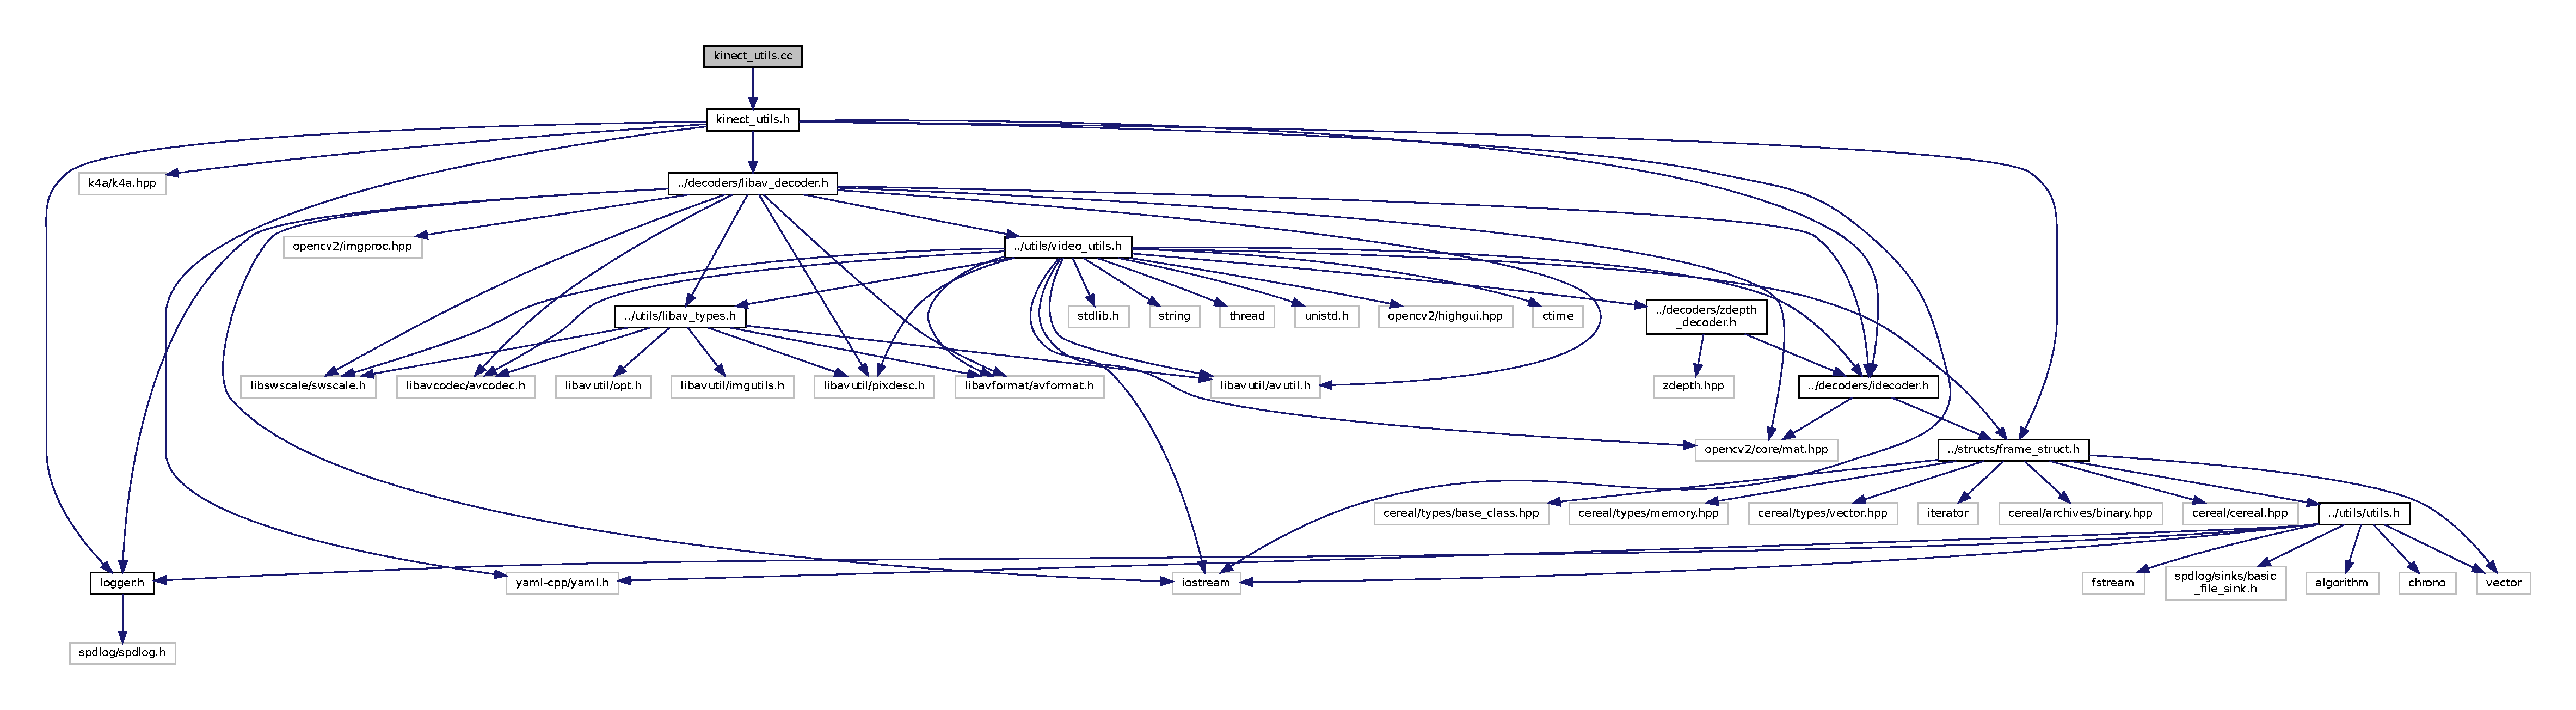
\includegraphics[width=350pt]{kinect__utils_8cc__incl}
\end{center}
\end{figure}
\subsection*{Namespaces}
\begin{DoxyCompactItemize}
\item 
 \hyperlink{namespacemoetsi_1_1ssp}{moetsi\+::ssp}
\begin{DoxyCompactList}\small\item\em Sensor Stream Pipe. \end{DoxyCompactList}\end{DoxyCompactItemize}
\subsection*{Functions}
\begin{DoxyCompactItemize}
\item 
Extended\+Azure\+Config \hyperlink{namespacemoetsi_1_1ssp_a357441ccde272e5d06fb708b62efa5c1}{moetsi\+::ssp\+::\+Build\+Kinect\+Config\+From\+Y\+A\+ML} (Y\+A\+M\+L\+::\+Node config)
\begin{DoxyCompactList}\small\item\em Build Kinect configuration from Y\+A\+ML configuration. \end{DoxyCompactList}\item 
void \hyperlink{namespacemoetsi_1_1ssp_aa91f7040cdd17f24ad6760aa1bdb428d}{moetsi\+::ssp\+::\+Frame\+Struct\+To\+K4A} (std\+::vector$<$ \hyperlink{structFrameStruct}{Frame\+Struct} $>$ \&f, k4a\+::capture \&sensor\+\_\+capture, std\+::unordered\+\_\+map$<$ std\+::string, std\+::shared\+\_\+ptr$<$ I\+Decoder $>$$>$ \&decoders)
\begin{DoxyCompactList}\small\item\em Transform frame structure to K4A format Update decoder dictionary. \end{DoxyCompactList}\end{DoxyCompactItemize}


\subsection{Detailed Description}
Utils for Kinect RT integration. 


\hypertarget{kinect__utils_8h}{}\doxysection{kinect\+\_\+utils.\+h File Reference}
\label{kinect__utils_8h}\index{kinect\_utils.h@{kinect\_utils.h}}


Utils for Kinect RT integration.  


{\ttfamily \#include $<$iostream$>$}\newline
{\ttfamily \#include $<$k4a/k4a.\+hpp$>$}\newline
{\ttfamily \#include $<$yaml-\/cpp/yaml.\+h$>$}\newline
{\ttfamily \#include \char`\"{}../decoders/idecoder.\+h\char`\"{}}\newline
{\ttfamily \#include \char`\"{}../decoders/libav\+\_\+decoder.\+h\char`\"{}}\newline
{\ttfamily \#include \char`\"{}../structs/frame\+\_\+struct.\+h\char`\"{}}\newline
{\ttfamily \#include \char`\"{}logger.\+h\char`\"{}}\newline
Include dependency graph for kinect\+\_\+utils.\+h\+:
% FIG 0
This graph shows which files directly or indirectly include this file\+:
% FIG 1
\doxysubsection*{Classes}
\begin{DoxyCompactItemize}
\item 
struct \mbox{\hyperlink{structmoetsi_1_1ssp_1_1ExtendedAzureConfig}{moetsi\+::ssp\+::\+Extended\+Azure\+Config}}
\begin{DoxyCompactList}\small\item\em Azure Kinect configuration. \end{DoxyCompactList}\end{DoxyCompactItemize}
\doxysubsection*{Namespaces}
\begin{DoxyCompactItemize}
\item 
 \mbox{\hyperlink{namespacemoetsi}{moetsi}}
\begin{DoxyCompactList}\small\item\em Moetsi creations. \end{DoxyCompactList}\item 
 \mbox{\hyperlink{namespacemoetsi_1_1ssp}{moetsi\+::ssp}}
\begin{DoxyCompactList}\small\item\em Sensor Stream Pipe. \end{DoxyCompactList}\end{DoxyCompactItemize}
\doxysubsection*{Functions}
\begin{DoxyCompactItemize}
\item 
Extended\+Azure\+Config \mbox{\hyperlink{namespacemoetsi_1_1ssp_a357441ccde272e5d06fb708b62efa5c1}{moetsi\+::ssp\+::\+Build\+Kinect\+Config\+From\+Y\+A\+ML}} (Y\+A\+M\+L\+::\+Node config)
\begin{DoxyCompactList}\small\item\em Build Kinect configuration from Y\+A\+ML configuration. \end{DoxyCompactList}\item 
void \mbox{\hyperlink{namespacemoetsi_1_1ssp_aa91f7040cdd17f24ad6760aa1bdb428d}{moetsi\+::ssp\+::\+Frame\+Struct\+To\+K4A}} (std\+::vector$<$ Frame\+Struct $>$ \&f, k4a\+::capture \&sensor\+\_\+capture, std\+::unordered\+\_\+map$<$ std\+::string, std\+::shared\+\_\+ptr$<$ I\+Decoder $>$$>$ \&decoders)
\begin{DoxyCompactList}\small\item\em Transform frame structure to K4A format Update decoder dictionary. \end{DoxyCompactList}\end{DoxyCompactItemize}


\doxysubsection{Detailed Description}
Utils for Kinect RT integration. 


\hypertarget{libav__decoder_8cc}{}\section{libav\+\_\+decoder.\+cc File Reference}
\label{libav__decoder_8cc}\index{libav\+\_\+decoder.\+cc@{libav\+\_\+decoder.\+cc}}


Jpeg/\+Mpeg decoder.  


{\ttfamily \#include \char`\"{}libav\+\_\+decoder.\+h\char`\"{}}\newline
Include dependency graph for libav\+\_\+decoder.\+cc\+:
\nopagebreak
\begin{figure}[H]
\begin{center}
\leavevmode
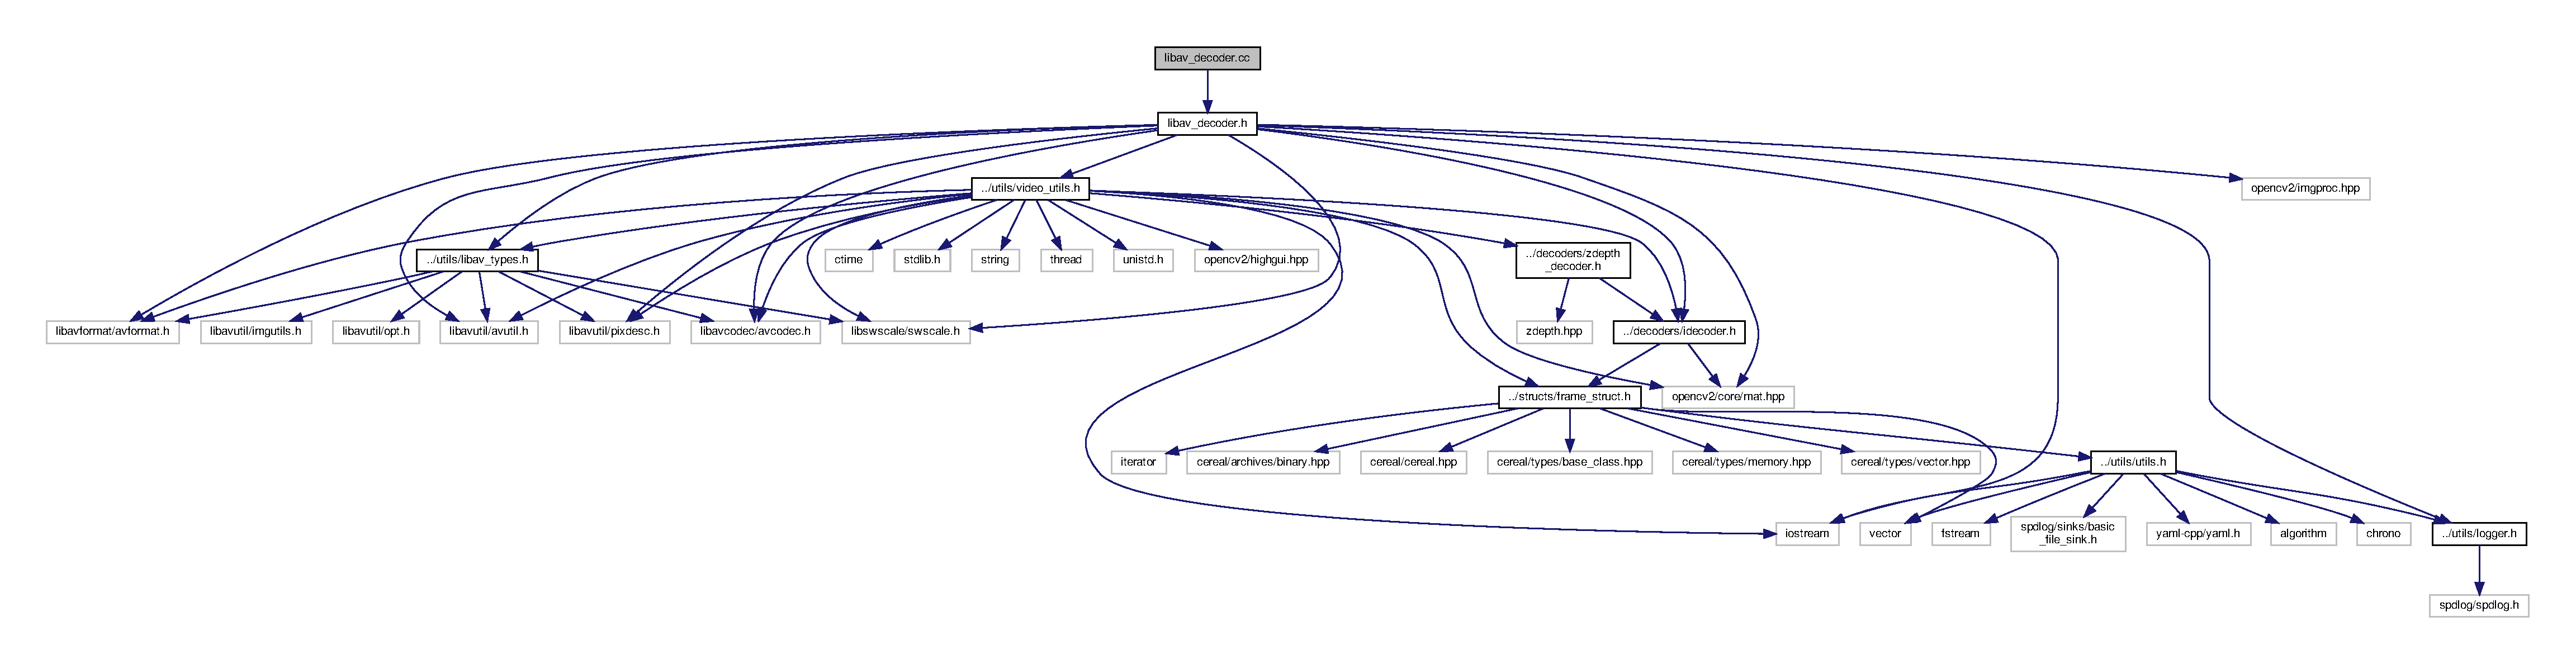
\includegraphics[width=350pt]{libav__decoder_8cc__incl}
\end{center}
\end{figure}
\subsection*{Namespaces}
\begin{DoxyCompactItemize}
\item 
 \hyperlink{namespacemoetsi_1_1ssp}{moetsi\+::ssp}
\begin{DoxyCompactList}\small\item\em Sensor Stream Pipe. \end{DoxyCompactList}\end{DoxyCompactItemize}


\subsection{Detailed Description}
Jpeg/\+Mpeg decoder. 


\hypertarget{libav__decoder_8h}{}\doxysection{libav\+\_\+decoder.\+h File Reference}
\label{libav__decoder_8h}\index{libav\_decoder.h@{libav\_decoder.h}}


Jpeg/\+Mpeg decoder.  


{\ttfamily \#include $<$libavcodec/avcodec.\+h$>$}\newline
{\ttfamily \#include $<$libavformat/avformat.\+h$>$}\newline
{\ttfamily \#include $<$libavutil/avutil.\+h$>$}\newline
{\ttfamily \#include $<$libavutil/pixdesc.\+h$>$}\newline
{\ttfamily \#include $<$libswscale/swscale.\+h$>$}\newline
{\ttfamily \#include \char`\"{}../utils/logger.\+h\char`\"{}}\newline
{\ttfamily \#include $<$iostream$>$}\newline
{\ttfamily \#include $<$opencv2/core/mat.\+hpp$>$}\newline
{\ttfamily \#include $<$opencv2/imgproc.\+hpp$>$}\newline
{\ttfamily \#include \char`\"{}../utils/video\+\_\+utils.\+h\char`\"{}}\newline
{\ttfamily \#include \char`\"{}../utils/libav\+\_\+types.\+h\char`\"{}}\newline
{\ttfamily \#include \char`\"{}idecoder.\+h\char`\"{}}\newline
Include dependency graph for libav\+\_\+decoder.\+h\+:
% FIG 0
This graph shows which files directly or indirectly include this file\+:
% FIG 1
\doxysubsection*{Classes}
\begin{DoxyCompactItemize}
\item 
class \mbox{\hyperlink{classmoetsi_1_1ssp_1_1LibAvDecoder}{moetsi\+::ssp\+::\+Lib\+Av\+Decoder}}
\begin{DoxyCompactList}\small\item\em AV (Jpeg/\+Mpeg) decoder. \end{DoxyCompactList}\end{DoxyCompactItemize}
\doxysubsection*{Namespaces}
\begin{DoxyCompactItemize}
\item 
 \mbox{\hyperlink{namespacemoetsi}{moetsi}}
\begin{DoxyCompactList}\small\item\em Moetsi creations. \end{DoxyCompactList}\item 
 \mbox{\hyperlink{namespacemoetsi_1_1ssp}{moetsi\+::ssp}}
\begin{DoxyCompactList}\small\item\em Sensor Stream Pipe. \end{DoxyCompactList}\end{DoxyCompactItemize}


\doxysubsection{Detailed Description}
Jpeg/\+Mpeg decoder. 


\hypertarget{libav__encoder_8cc}{}\section{libav\+\_\+encoder.\+cc File Reference}
\label{libav__encoder_8cc}\index{libav\+\_\+encoder.\+cc@{libav\+\_\+encoder.\+cc}}


Jpef/\+Mpeg encoder.  


{\ttfamily \#include \char`\"{}libav\+\_\+encoder.\+h\char`\"{}}\newline
Include dependency graph for libav\+\_\+encoder.\+cc\+:
\nopagebreak
\begin{figure}[H]
\begin{center}
\leavevmode
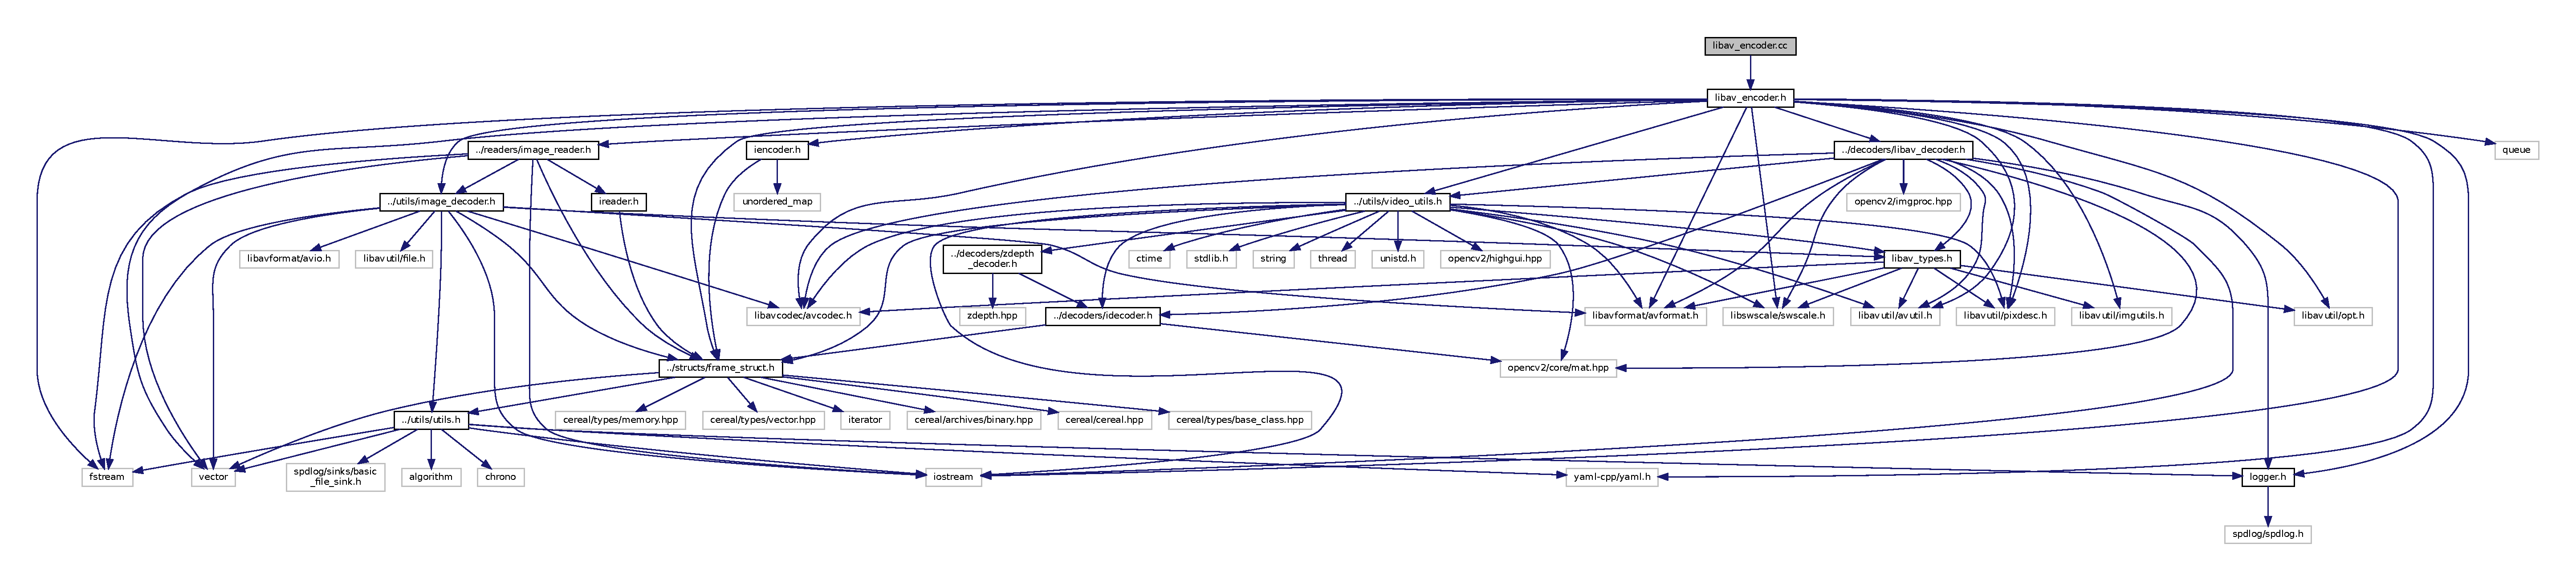
\includegraphics[width=350pt]{libav__encoder_8cc__incl}
\end{center}
\end{figure}
\subsection*{Namespaces}
\begin{DoxyCompactItemize}
\item 
 \hyperlink{namespacemoetsi_1_1ssp}{moetsi\+::ssp}
\begin{DoxyCompactList}\small\item\em Sensor Stream Pipe. \end{DoxyCompactList}\end{DoxyCompactItemize}


\subsection{Detailed Description}
Jpef/\+Mpeg encoder. 


\hypertarget{libav__encoder_8h}{}\doxysection{libav\+\_\+encoder.\+h File Reference}
\label{libav__encoder_8h}\index{libav\_encoder.h@{libav\_encoder.h}}


Jpeg/\+Mpeg encoder.  


{\ttfamily \#include $<$fstream$>$}\newline
{\ttfamily \#include $<$iostream$>$}\newline
{\ttfamily \#include $<$queue$>$}\newline
{\ttfamily \#include $<$vector$>$}\newline
{\ttfamily \#include $<$yaml-\/cpp/yaml.\+h$>$}\newline
{\ttfamily \#include $<$libavcodec/avcodec.\+h$>$}\newline
{\ttfamily \#include $<$libavformat/avformat.\+h$>$}\newline
{\ttfamily \#include $<$libavutil/avutil.\+h$>$}\newline
{\ttfamily \#include $<$libavutil/imgutils.\+h$>$}\newline
{\ttfamily \#include $<$libavutil/opt.\+h$>$}\newline
{\ttfamily \#include $<$libavutil/pixdesc.\+h$>$}\newline
{\ttfamily \#include $<$libswscale/swscale.\+h$>$}\newline
{\ttfamily \#include \char`\"{}../readers/image\+\_\+reader.\+h\char`\"{}}\newline
{\ttfamily \#include \char`\"{}../structs/frame\+\_\+struct.\+h\char`\"{}}\newline
{\ttfamily \#include \char`\"{}../utils/image\+\_\+decoder.\+h\char`\"{}}\newline
{\ttfamily \#include \char`\"{}../utils/video\+\_\+utils.\+h\char`\"{}}\newline
{\ttfamily \#include \char`\"{}iencoder.\+h\char`\"{}}\newline
{\ttfamily \#include \char`\"{}../decoders/libav\+\_\+decoder.\+h\char`\"{}}\newline
{\ttfamily \#include \char`\"{}../utils/logger.\+h\char`\"{}}\newline
Include dependency graph for libav\+\_\+encoder.\+h\+:
\nopagebreak
\begin{figure}[H]
\begin{center}
\leavevmode
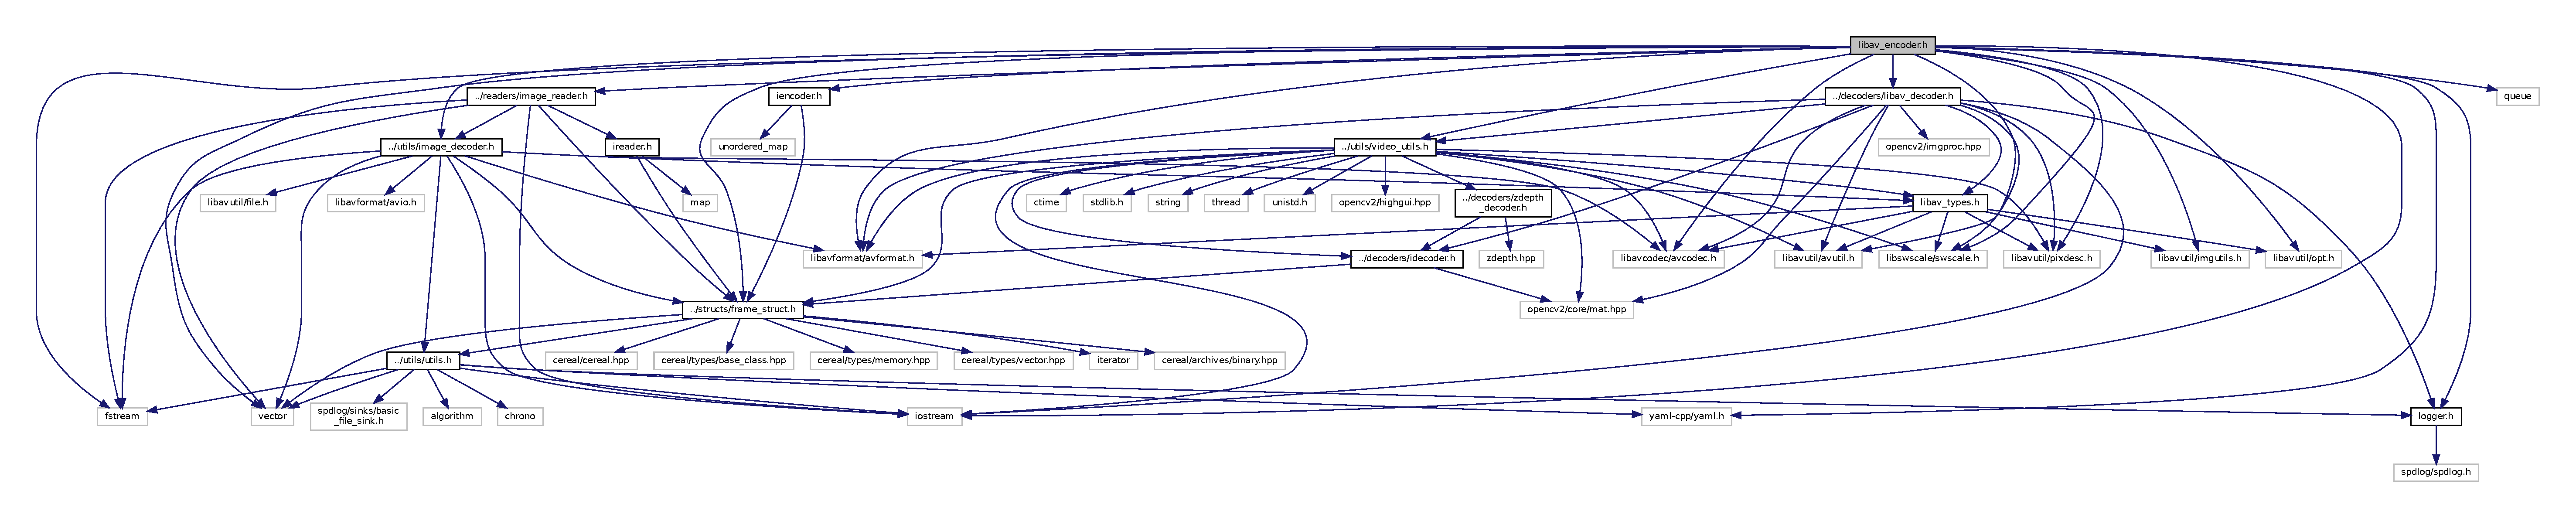
\includegraphics[width=350pt]{libav__encoder_8h__incl}
\end{center}
\end{figure}
This graph shows which files directly or indirectly include this file\+:
\nopagebreak
\begin{figure}[H]
\begin{center}
\leavevmode
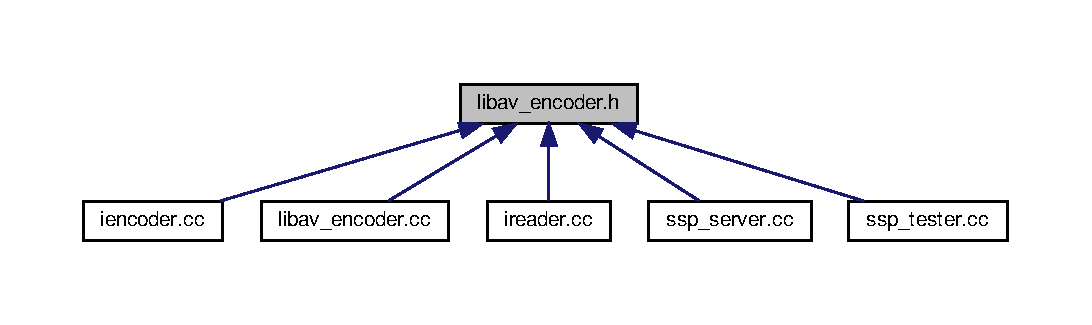
\includegraphics[width=350pt]{libav__encoder_8h__dep__incl}
\end{center}
\end{figure}
\doxysubsection*{Classes}
\begin{DoxyCompactItemize}
\item 
class \mbox{\hyperlink{classmoetsi_1_1ssp_1_1LibAvEncoder}{moetsi\+::ssp\+::\+Lib\+Av\+Encoder}}
\begin{DoxyCompactList}\small\item\em Lib\+AV encoder for Jpeg/\+Mpeg. \end{DoxyCompactList}\end{DoxyCompactItemize}
\doxysubsection*{Namespaces}
\begin{DoxyCompactItemize}
\item 
 \mbox{\hyperlink{namespacemoetsi}{moetsi}}
\begin{DoxyCompactList}\small\item\em Moetsi creations. \end{DoxyCompactList}\item 
 \mbox{\hyperlink{namespacemoetsi_1_1ssp}{moetsi\+::ssp}}
\begin{DoxyCompactList}\small\item\em Sensor Stream Pipe. \end{DoxyCompactList}\end{DoxyCompactItemize}


\doxysubsection{Detailed Description}
Jpeg/\+Mpeg encoder. 


\hypertarget{logger_8h}{}\section{logger.\+h File Reference}
\label{logger_8h}\index{logger.\+h@{logger.\+h}}


Logger header.  


{\ttfamily \#include $<$spdlog/spdlog.\+h$>$}\newline
Include dependency graph for logger.\+h\+:
\nopagebreak
\begin{figure}[H]
\begin{center}
\leavevmode
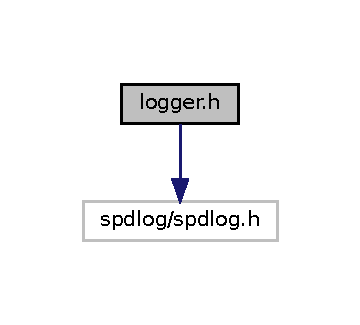
\includegraphics[width=165pt]{logger_8h__incl}
\end{center}
\end{figure}
This graph shows which files directly or indirectly include this file\+:
\nopagebreak
\begin{figure}[H]
\begin{center}
\leavevmode
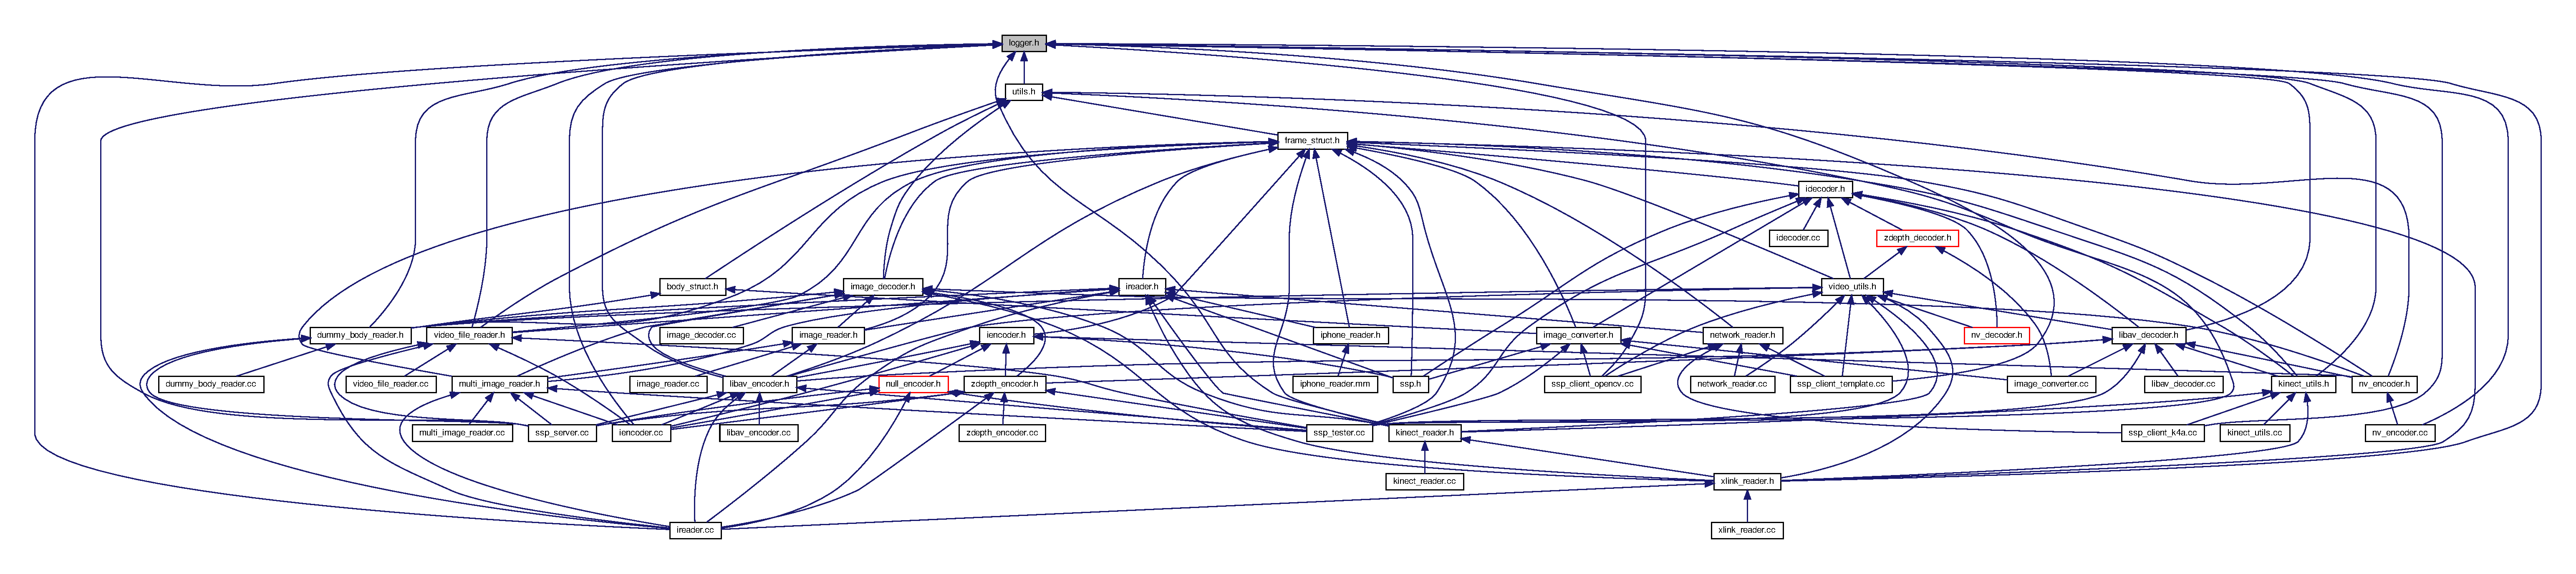
\includegraphics[width=350pt]{logger_8h__dep__incl}
\end{center}
\end{figure}


\subsection{Detailed Description}
Logger header. 


\hypertarget{multi__image__reader_8cc}{}\doxysection{multi\+\_\+image\+\_\+reader.\+cc File Reference}
\label{multi__image__reader_8cc}\index{multi\_image\_reader.cc@{multi\_image\_reader.cc}}


Multi image reader.  


{\ttfamily \#include \char`\"{}multi\+\_\+image\+\_\+reader.\+h\char`\"{}}\newline
Include dependency graph for multi\+\_\+image\+\_\+reader.\+cc\+:
\nopagebreak
\begin{figure}[H]
\begin{center}
\leavevmode
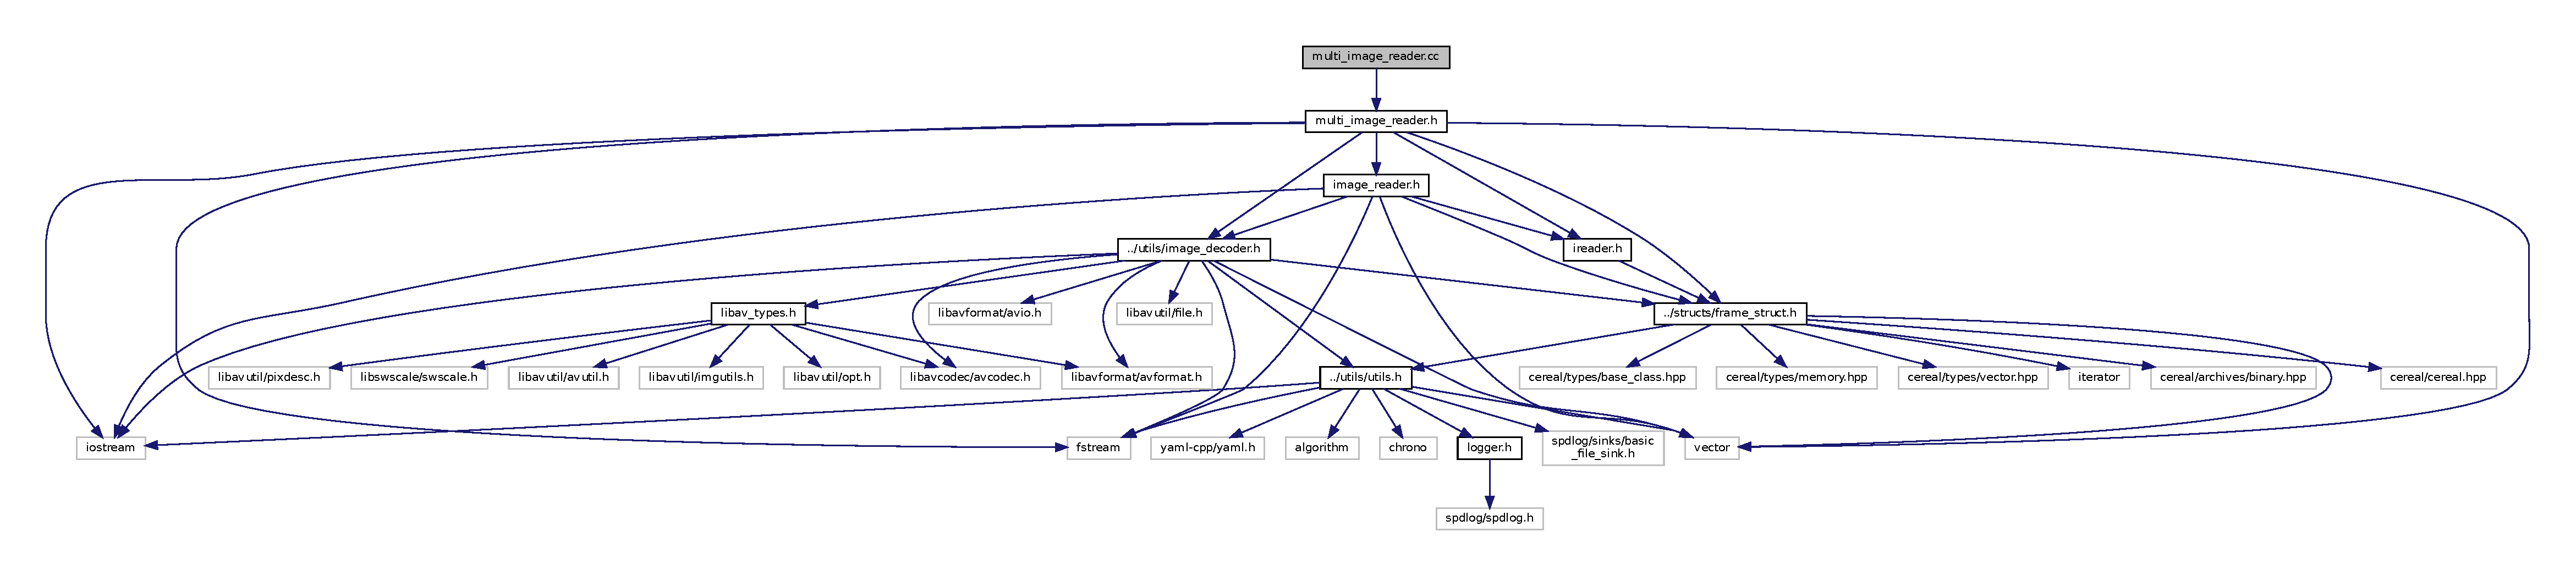
\includegraphics[width=350pt]{multi__image__reader_8cc__incl}
\end{center}
\end{figure}
\doxysubsection*{Namespaces}
\begin{DoxyCompactItemize}
\item 
 \mbox{\hyperlink{namespacemoetsi}{moetsi}}
\begin{DoxyCompactList}\small\item\em Moetsi creations. \end{DoxyCompactList}\item 
 \mbox{\hyperlink{namespacemoetsi_1_1ssp}{moetsi\+::ssp}}
\begin{DoxyCompactList}\small\item\em Sensor Stream Pipe. \end{DoxyCompactList}\end{DoxyCompactItemize}


\doxysubsection{Detailed Description}
Multi image reader. 


\hypertarget{multi__image__reader_8h}{}\doxysection{multi\+\_\+image\+\_\+reader.\+h File Reference}
\label{multi__image__reader_8h}\index{multi\_image\_reader.h@{multi\_image\_reader.h}}


Multi image reader.  


{\ttfamily \#include $<$fstream$>$}\newline
{\ttfamily \#include $<$iostream$>$}\newline
{\ttfamily \#include $<$vector$>$}\newline
{\ttfamily \#include \char`\"{}../structs/frame\+\_\+struct.\+h\char`\"{}}\newline
{\ttfamily \#include \char`\"{}../utils/image\+\_\+decoder.\+h\char`\"{}}\newline
{\ttfamily \#include \char`\"{}image\+\_\+reader.\+h\char`\"{}}\newline
{\ttfamily \#include \char`\"{}ireader.\+h\char`\"{}}\newline
Include dependency graph for multi\+\_\+image\+\_\+reader.\+h\+:
\nopagebreak
\begin{figure}[H]
\begin{center}
\leavevmode
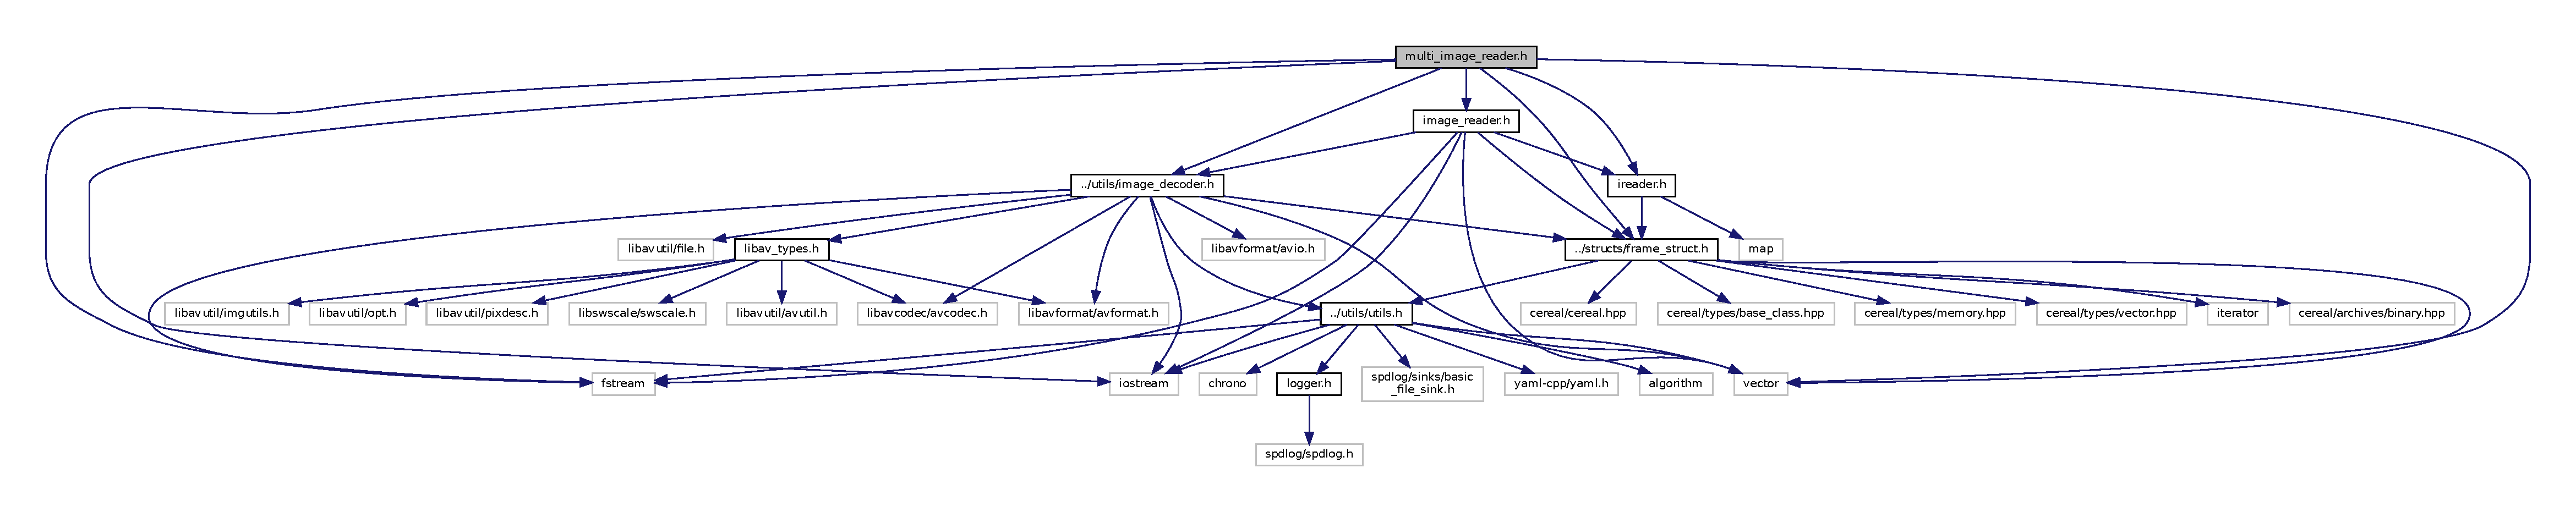
\includegraphics[width=350pt]{multi__image__reader_8h__incl}
\end{center}
\end{figure}
This graph shows which files directly or indirectly include this file\+:
\nopagebreak
\begin{figure}[H]
\begin{center}
\leavevmode
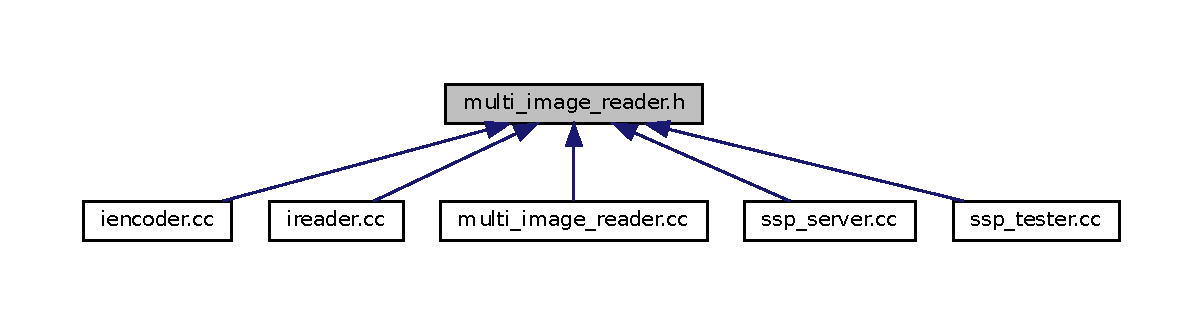
\includegraphics[width=350pt]{multi__image__reader_8h__dep__incl}
\end{center}
\end{figure}
\doxysubsection*{Classes}
\begin{DoxyCompactItemize}
\item 
class \mbox{\hyperlink{classmoetsi_1_1ssp_1_1MultiImageReader}{moetsi\+::ssp\+::\+Multi\+Image\+Reader}}
\end{DoxyCompactItemize}
\doxysubsection*{Namespaces}
\begin{DoxyCompactItemize}
\item 
 \mbox{\hyperlink{namespacemoetsi}{moetsi}}
\begin{DoxyCompactList}\small\item\em Moetsi creations. \end{DoxyCompactList}\item 
 \mbox{\hyperlink{namespacemoetsi_1_1ssp}{moetsi\+::ssp}}
\begin{DoxyCompactList}\small\item\em Sensor Stream Pipe. \end{DoxyCompactList}\end{DoxyCompactItemize}


\doxysubsection{Detailed Description}
Multi image reader. 


\hypertarget{network__reader_8cc}{}\doxysection{network\+\_\+reader.\+cc File Reference}
\label{network__reader_8cc}\index{network\_reader.cc@{network\_reader.cc}}


Network reader.  


{\ttfamily \#include \char`\"{}network\+\_\+reader.\+h\char`\"{}}\newline
{\ttfamily \#include \char`\"{}../utils/video\+\_\+utils.\+h\char`\"{}}\newline
Include dependency graph for network\+\_\+reader.\+cc\+:
% FIG 0
\doxysubsection*{Namespaces}
\begin{DoxyCompactItemize}
\item 
 \mbox{\hyperlink{namespacemoetsi}{moetsi}}
\begin{DoxyCompactList}\small\item\em Moetsi creations. \end{DoxyCompactList}\item 
 \mbox{\hyperlink{namespacemoetsi_1_1ssp}{moetsi\+::ssp}}
\begin{DoxyCompactList}\small\item\em Sensor Stream Pipe. \end{DoxyCompactList}\end{DoxyCompactItemize}
\doxysubsection*{Functions}
\begin{DoxyCompactItemize}
\item 
\mbox{\Hypertarget{namespacemoetsi_1_1ssp_a884aae59668e7913051f2875b047688e}\label{namespacemoetsi_1_1ssp_a884aae59668e7913051f2875b047688e}} 
unsigned long {\bfseries moetsi\+::ssp\+::elapsed} (unsigned long start, unsigned long end)
\end{DoxyCompactItemize}


\doxysubsection{Detailed Description}
Network reader. 


\hypertarget{network__reader_8h}{}\section{network\+\_\+reader.\+h File Reference}
\label{network__reader_8h}\index{network\+\_\+reader.\+h@{network\+\_\+reader.\+h}}


Network reader.  


{\ttfamily \#include $<$zmq.\+hpp$>$}\newline
{\ttfamily \#include \char`\"{}../structs/frame\+\_\+struct.\+h\char`\"{}}\newline
{\ttfamily \#include \char`\"{}ireader.\+h\char`\"{}}\newline
Include dependency graph for network\+\_\+reader.\+h\+:
\nopagebreak
\begin{figure}[H]
\begin{center}
\leavevmode
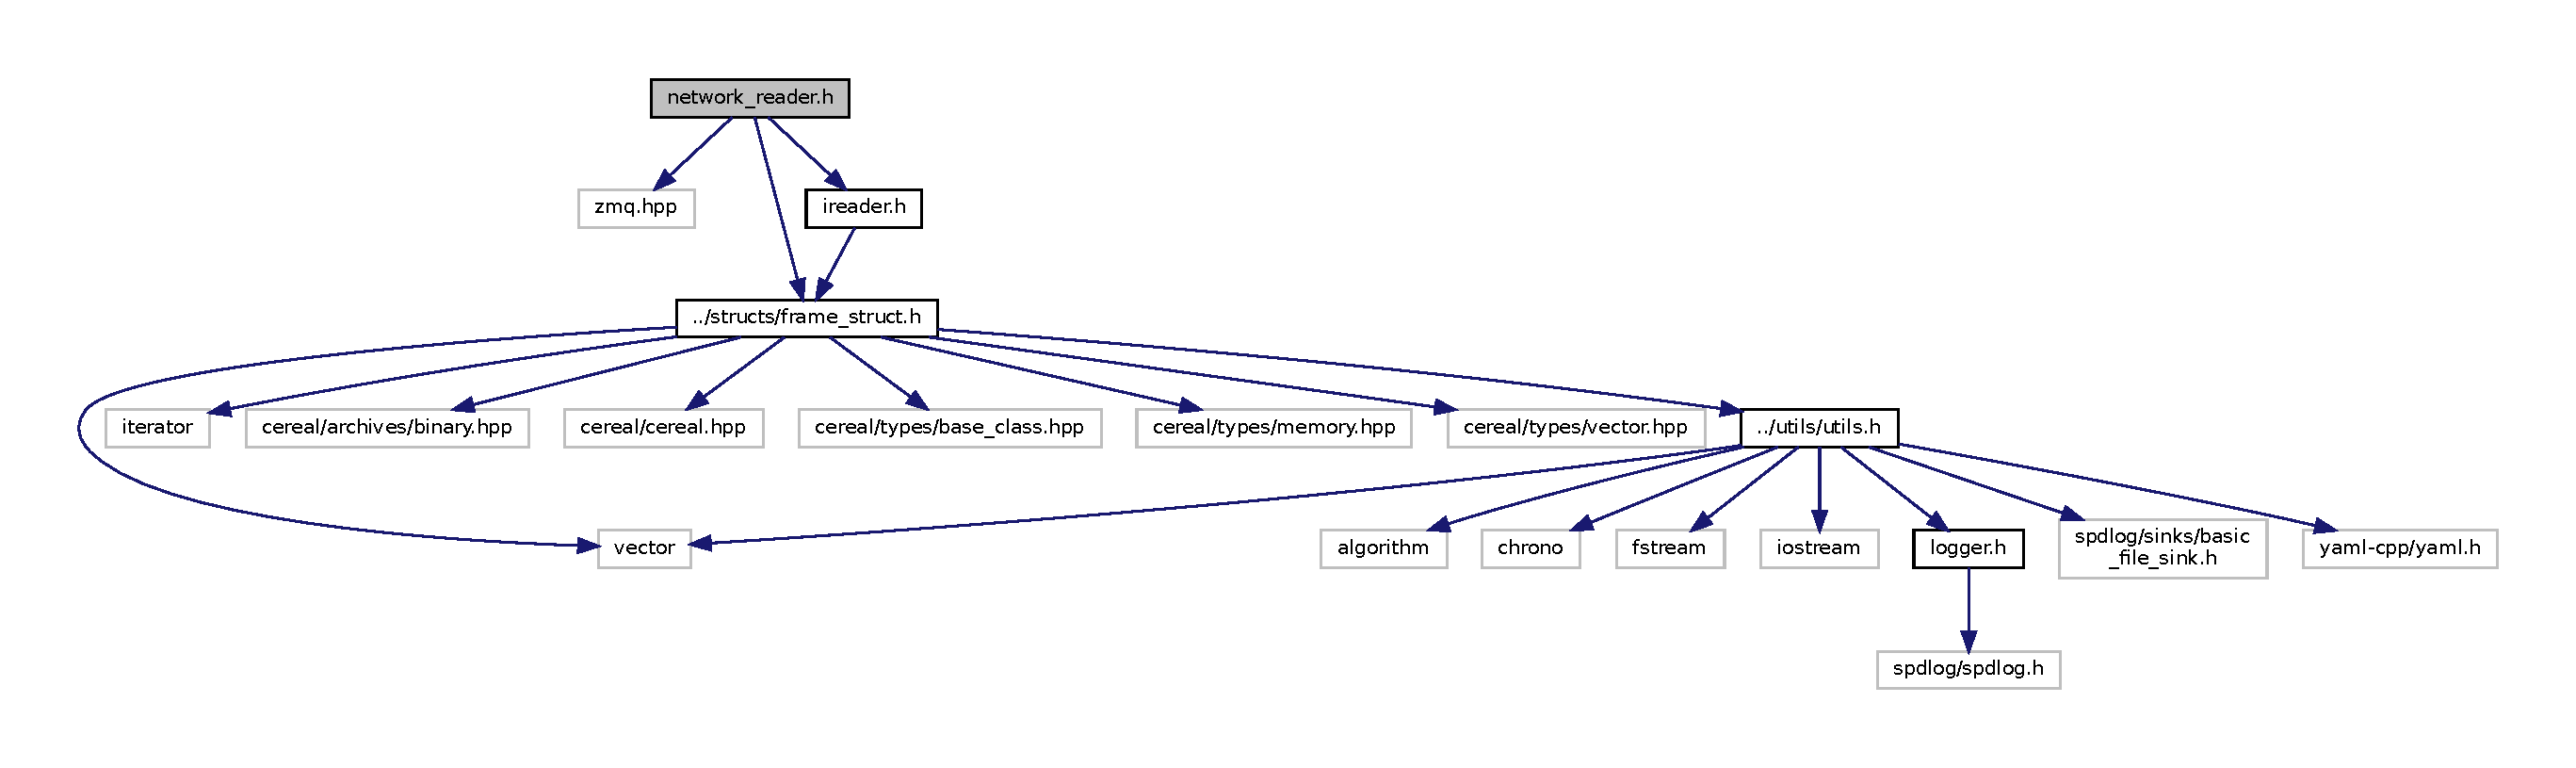
\includegraphics[width=350pt]{network__reader_8h__incl}
\end{center}
\end{figure}
This graph shows which files directly or indirectly include this file\+:
\nopagebreak
\begin{figure}[H]
\begin{center}
\leavevmode
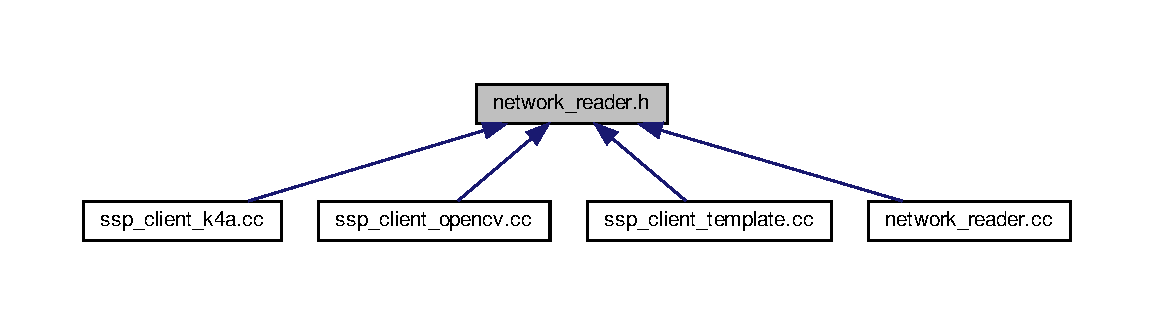
\includegraphics[width=350pt]{network__reader_8h__dep__incl}
\end{center}
\end{figure}
\subsection*{Classes}
\begin{DoxyCompactItemize}
\item 
class \hyperlink{classmoetsi_1_1ssp_1_1NetworkReader}{moetsi\+::ssp\+::\+Network\+Reader}
\begin{DoxyCompactList}\small\item\em Network reader. \end{DoxyCompactList}\end{DoxyCompactItemize}
\subsection*{Namespaces}
\begin{DoxyCompactItemize}
\item 
 \hyperlink{namespacemoetsi_1_1ssp}{moetsi\+::ssp}
\begin{DoxyCompactList}\small\item\em Sensor Stream Pipe. \end{DoxyCompactList}\end{DoxyCompactItemize}
\subsection*{Macros}
\begin{DoxyCompactItemize}
\item 
\mbox{\Hypertarget{network__reader_8h_ae185e948f0542226cd0c076cd159576c}\label{network__reader_8h_ae185e948f0542226cd0c076cd159576c}} 
\#define {\bfseries P\+O\+L\+L\+\_\+\+T\+I\+M\+E\+O\+U\+T\+\_\+\+MS}~500
\end{DoxyCompactItemize}


\subsection{Detailed Description}
Network reader. 


\hypertarget{null__encoder_8cc}{}\doxysection{null\+\_\+encoder.\+cc File Reference}
\label{null__encoder_8cc}\index{null\_encoder.cc@{null\_encoder.cc}}


Straight pipe encoder.  


{\ttfamily \#include \char`\"{}null\+\_\+encoder.\+h\char`\"{}}\newline
Include dependency graph for null\+\_\+encoder.\+cc\+:
\nopagebreak
\begin{figure}[H]
\begin{center}
\leavevmode
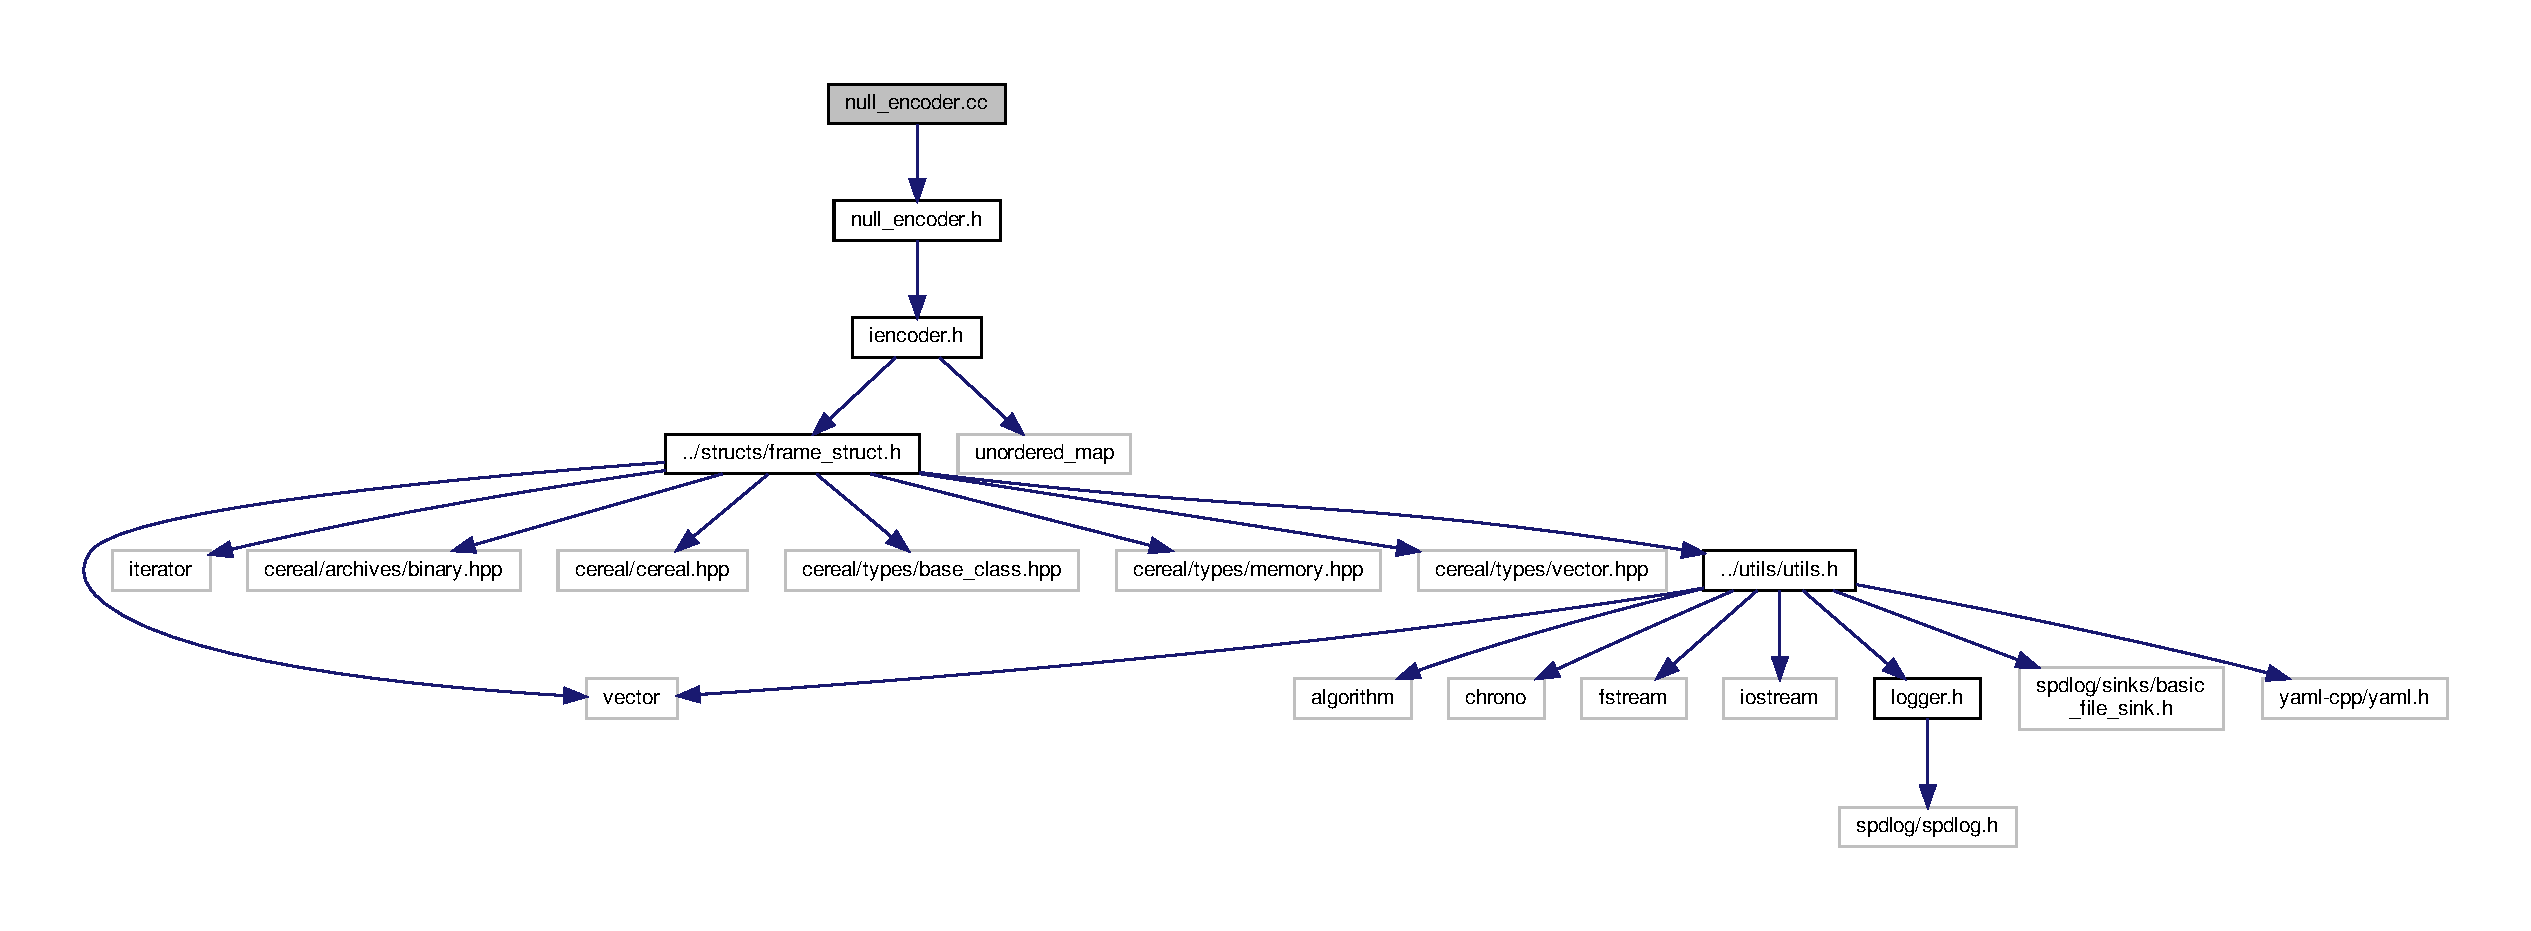
\includegraphics[width=350pt]{null__encoder_8cc__incl}
\end{center}
\end{figure}
\doxysubsection*{Namespaces}
\begin{DoxyCompactItemize}
\item 
 \mbox{\hyperlink{namespacemoetsi}{moetsi}}
\begin{DoxyCompactList}\small\item\em Moetsi creations. \end{DoxyCompactList}\item 
 \mbox{\hyperlink{namespacemoetsi_1_1ssp}{moetsi\+::ssp}}
\begin{DoxyCompactList}\small\item\em Sensor Stream Pipe. \end{DoxyCompactList}\end{DoxyCompactItemize}


\doxysubsection{Detailed Description}
Straight pipe encoder. 


\hypertarget{null__encoder_8h}{}\doxysection{null\+\_\+encoder.\+h File Reference}
\label{null__encoder_8h}\index{null\_encoder.h@{null\_encoder.h}}
{\ttfamily \#include \char`\"{}iencoder.\+h\char`\"{}}\newline
Include dependency graph for null\+\_\+encoder.\+h\+:
% FIG 0
This graph shows which files directly or indirectly include this file\+:
% FIG 1
\doxysubsection*{Classes}
\begin{DoxyCompactItemize}
\item 
class \mbox{\hyperlink{classmoetsi_1_1ssp_1_1NullEncoder}{moetsi\+::ssp\+::\+Null\+Encoder}}
\begin{DoxyCompactList}\small\item\em Nullencoder Straight pipe encoder. \end{DoxyCompactList}\end{DoxyCompactItemize}
\doxysubsection*{Namespaces}
\begin{DoxyCompactItemize}
\item 
 \mbox{\hyperlink{namespacemoetsi}{moetsi}}
\begin{DoxyCompactList}\small\item\em Moetsi creations. \end{DoxyCompactList}\item 
 \mbox{\hyperlink{namespacemoetsi_1_1ssp}{moetsi\+::ssp}}
\begin{DoxyCompactList}\small\item\em Sensor Stream Pipe. \end{DoxyCompactList}\end{DoxyCompactItemize}


\doxysubsection{Detailed Description}
@breif Straight pipe encoder 
\hypertarget{nv__decoder_8cc}{}\doxysection{nv\+\_\+decoder.\+cc File Reference}
\label{nv__decoder_8cc}\index{nv\_decoder.cc@{nv\_decoder.cc}}


Nv\+Pipe decoder.  


{\ttfamily \#include \char`\"{}nv\+\_\+decoder.\+h\char`\"{}}\newline
Include dependency graph for nv\+\_\+decoder.\+cc\+:
% FIG 0
\doxysubsection*{Namespaces}
\begin{DoxyCompactItemize}
\item 
 \mbox{\hyperlink{namespacemoetsi}{moetsi}}
\begin{DoxyCompactList}\small\item\em Moetsi creations. \end{DoxyCompactList}\item 
 \mbox{\hyperlink{namespacemoetsi_1_1ssp}{moetsi\+::ssp}}
\begin{DoxyCompactList}\small\item\em Sensor Stream Pipe. \end{DoxyCompactList}\end{DoxyCompactItemize}


\doxysubsection{Detailed Description}
Nv\+Pipe decoder. 


\hypertarget{nv__decoder_8h}{}\doxysection{nv\+\_\+decoder.\+h File Reference}
\label{nv__decoder_8h}\index{nv\_decoder.h@{nv\_decoder.h}}


Nv\+Pipe decoder.  


{\ttfamily \#include $<$Nv\+Pipe.\+h$>$}\newline
{\ttfamily \#include $<$iostream$>$}\newline
{\ttfamily \#include $<$opencv2/core/mat.\+hpp$>$}\newline
{\ttfamily \#include \char`\"{}../utils/nvpipe\+\_\+types.\+h\char`\"{}}\newline
{\ttfamily \#include \char`\"{}../utils/video\+\_\+utils.\+h\char`\"{}}\newline
{\ttfamily \#include \char`\"{}idecoder.\+h\char`\"{}}\newline
Include dependency graph for nv\+\_\+decoder.\+h\+:
% FIG 0
This graph shows which files directly or indirectly include this file\+:
% FIG 1
\doxysubsection*{Classes}
\begin{DoxyCompactItemize}
\item 
class \mbox{\hyperlink{classmoetsi_1_1ssp_1_1NvDecoder}{moetsi\+::ssp\+::\+Nv\+Decoder}}
\begin{DoxyCompactList}\small\item\em Nv\+Pipe decoder. \end{DoxyCompactList}\end{DoxyCompactItemize}
\doxysubsection*{Namespaces}
\begin{DoxyCompactItemize}
\item 
 \mbox{\hyperlink{namespacemoetsi}{moetsi}}
\begin{DoxyCompactList}\small\item\em Moetsi creations. \end{DoxyCompactList}\item 
 \mbox{\hyperlink{namespacemoetsi_1_1ssp}{moetsi\+::ssp}}
\begin{DoxyCompactList}\small\item\em Sensor Stream Pipe. \end{DoxyCompactList}\end{DoxyCompactItemize}


\doxysubsection{Detailed Description}
Nv\+Pipe decoder. 


\hypertarget{nv__encoder_8cc}{}\doxysection{nv\+\_\+encoder.\+cc File Reference}
\label{nv__encoder_8cc}\index{nv\_encoder.cc@{nv\_encoder.cc}}


Nv\+Pipe encoder.  


{\ttfamily \#include $<$unistd.\+h$>$}\newline
{\ttfamily \#include \char`\"{}../utils/logger.\+h\char`\"{}}\newline
{\ttfamily \#include $<$ctime$>$}\newline
{\ttfamily \#include $<$iostream$>$}\newline
{\ttfamily \#include $<$stdlib.\+h$>$}\newline
{\ttfamily \#include $<$string$>$}\newline
{\ttfamily \#include $<$thread$>$}\newline
{\ttfamily \#include $<$opencv2/imgproc.\+hpp$>$}\newline
{\ttfamily \#include $<$yaml-\/cpp/yaml.\+h$>$}\newline
{\ttfamily \#include \char`\"{}nv\+\_\+encoder.\+h\char`\"{}}\newline
Include dependency graph for nv\+\_\+encoder.\+cc\+:
% FIG 0
\doxysubsection*{Namespaces}
\begin{DoxyCompactItemize}
\item 
 \mbox{\hyperlink{namespacemoetsi}{moetsi}}
\begin{DoxyCompactList}\small\item\em Moetsi creations. \end{DoxyCompactList}\item 
 \mbox{\hyperlink{namespacemoetsi_1_1ssp}{moetsi\+::ssp}}
\begin{DoxyCompactList}\small\item\em Sensor Stream Pipe. \end{DoxyCompactList}\end{DoxyCompactItemize}


\doxysubsection{Detailed Description}
Nv\+Pipe encoder. 


\hypertarget{nv__encoder_8h}{}\section{nv\+\_\+encoder.\+h File Reference}
\label{nv__encoder_8h}\index{nv\+\_\+encoder.\+h@{nv\+\_\+encoder.\+h}}


Nv\+Pipe encoder.  


{\ttfamily \#include $<$Nv\+Pipe.\+h$>$}\newline
{\ttfamily \#include $<$yaml-\/cpp/yaml.\+h$>$}\newline
{\ttfamily \#include \char`\"{}../decoders/libav\+\_\+decoder.\+h\char`\"{}}\newline
{\ttfamily \#include \char`\"{}../utils/image\+\_\+decoder.\+h\char`\"{}}\newline
{\ttfamily \#include \char`\"{}iencoder.\+h\char`\"{}}\newline
{\ttfamily \#include \char`\"{}../structs/frame\+\_\+struct.\+h\char`\"{}}\newline
{\ttfamily \#include \char`\"{}../utils/utils.\+h\char`\"{}}\newline
Include dependency graph for nv\+\_\+encoder.\+h\+:
\nopagebreak
\begin{figure}[H]
\begin{center}
\leavevmode
\includegraphics[width=350pt]{nv__encoder_8h__incl}
\end{center}
\end{figure}
This graph shows which files directly or indirectly include this file\+:
\nopagebreak
\begin{figure}[H]
\begin{center}
\leavevmode
\includegraphics[width=160pt]{nv__encoder_8h__dep__incl}
\end{center}
\end{figure}
\subsection*{Classes}
\begin{DoxyCompactItemize}
\item 
class \hyperlink{classmoetsi_1_1ssp_1_1NvEncoder}{moetsi\+::ssp\+::\+Nv\+Encoder}
\begin{DoxyCompactList}\small\item\em Nv\+Pipe encoder. \end{DoxyCompactList}\end{DoxyCompactItemize}
\subsection*{Namespaces}
\begin{DoxyCompactItemize}
\item 
 \hyperlink{namespacemoetsi_1_1ssp}{moetsi\+::ssp}
\begin{DoxyCompactList}\small\item\em Sensor Stream Pipe. \end{DoxyCompactList}\end{DoxyCompactItemize}


\subsection{Detailed Description}
Nv\+Pipe encoder. 


\hypertarget{nvpipe__types_8h}{}\section{nvpipe\+\_\+types.\+h File Reference}
\label{nvpipe__types_8h}\index{nvpipe\+\_\+types.\+h@{nvpipe\+\_\+types.\+h}}


Types for Nv\+Pipe support.  


{\ttfamily \#include $<$Nv\+Pipe.\+h$>$}\newline
{\ttfamily \#include $<$memory$>$}\newline
Include dependency graph for nvpipe\+\_\+types.\+h\+:
\nopagebreak
\begin{figure}[H]
\begin{center}
\leavevmode
\includegraphics[width=208pt]{nvpipe__types_8h__incl}
\end{center}
\end{figure}
This graph shows which files directly or indirectly include this file\+:
\nopagebreak
\begin{figure}[H]
\begin{center}
\leavevmode
\includegraphics[width=163pt]{nvpipe__types_8h__dep__incl}
\end{center}
\end{figure}
\subsection*{Classes}
\begin{DoxyCompactItemize}
\item 
struct \hyperlink{structmoetsi_1_1ssp_1_1NVPipeDeleter}{moetsi\+::ssp\+::\+N\+V\+Pipe\+Deleter}
\end{DoxyCompactItemize}
\subsection*{Namespaces}
\begin{DoxyCompactItemize}
\item 
 \hyperlink{namespacemoetsi_1_1ssp}{moetsi\+::ssp}
\begin{DoxyCompactList}\small\item\em Sensor Stream Pipe. \end{DoxyCompactList}\end{DoxyCompactItemize}
\subsection*{Typedefs}
\begin{DoxyCompactItemize}
\item 
\mbox{\Hypertarget{namespacemoetsi_1_1ssp_a9113dc526e642001a9213326b2c5539f}\label{namespacemoetsi_1_1ssp_a9113dc526e642001a9213326b2c5539f}} 
typedef std\+::unique\+\_\+ptr$<$ Nv\+Pipe, N\+V\+Pipe\+Deleter $>$ {\bfseries moetsi\+::ssp\+::\+Nv\+Pipe\+SafeP}
\end{DoxyCompactItemize}


\subsection{Detailed Description}
Types for Nv\+Pipe support. 


\hypertarget{similarity__measures_8h}{}\doxysection{similarity\+\_\+measures.\+h File Reference}
\label{similarity__measures_8h}\index{similarity\_measures.h@{similarity\_measures.h}}


Similarity measures.  


{\ttfamily \#include $<$opencv2/core/mat.\+hpp$>$}\newline
{\ttfamily \#include $<$opencv2/highgui.\+hpp$>$}\newline
Include dependency graph for similarity\+\_\+measures.\+h\+:
% FIG 0
This graph shows which files directly or indirectly include this file\+:
% FIG 1
\doxysubsection*{Namespaces}
\begin{DoxyCompactItemize}
\item 
 \mbox{\hyperlink{namespacemoetsi}{moetsi}}
\begin{DoxyCompactList}\small\item\em Moetsi creations. \end{DoxyCompactList}\item 
 \mbox{\hyperlink{namespacemoetsi_1_1ssp}{moetsi\+::ssp}}
\begin{DoxyCompactList}\small\item\em Sensor Stream Pipe. \end{DoxyCompactList}\end{DoxyCompactItemize}
\doxysubsection*{Functions}
\begin{DoxyCompactItemize}
\item 
double \mbox{\hyperlink{namespacemoetsi_1_1ssp_a0290f5110cb2cd2c9327c2fa6a528c84}{moetsi\+::ssp\+::\+Get\+P\+S\+NR}} (const Mat \&I1, const Mat \&I2, double max\+\_\+value)
\begin{DoxyCompactList}\small\item\em Get Peak Signal to Noise Ration similarity. \end{DoxyCompactList}\item 
double \mbox{\hyperlink{namespacemoetsi_1_1ssp_a3c49338af0ef5d208a34718fe29fc693}{moetsi\+::ssp\+::\+Get\+M\+SE}} (const Mat \&I1, const Mat \&I2)
\begin{DoxyCompactList}\small\item\em Get Mean Square Error (distance) between images. \end{DoxyCompactList}\item 
Scalar \mbox{\hyperlink{namespacemoetsi_1_1ssp_ae44d43d11d27495335b5494d0cff7601}{moetsi\+::ssp\+::\+Get\+M\+S\+S\+IM}} (const Mat \&i1, const Mat \&i2)
\begin{DoxyCompactList}\small\item\em Get Structural Similarity between 2 images cf. for instance \href{http://amroamroamro.github.io/mexopencv/opencv/image_similarity_demo.html}{\texttt{ http\+://amroamroamro.\+github.\+io/mexopencv/opencv/image\+\_\+similarity\+\_\+demo.\+html}} for a simple S\+S\+IM introduction. \end{DoxyCompactList}\end{DoxyCompactItemize}


\doxysubsection{Detailed Description}
Similarity measures. 


\hypertarget{ssp__client__k4a_8cc}{}\section{ssp\+\_\+client\+\_\+k4a.\+cc File Reference}
\label{ssp__client__k4a_8cc}\index{ssp\+\_\+client\+\_\+k4a.\+cc@{ssp\+\_\+client\+\_\+k4a.\+cc}}


S\+SP client with lib k4a.  


{\ttfamily \#include $<$chrono$>$}\newline
{\ttfamily \#include $<$iostream$>$}\newline
{\ttfamily \#include $<$mutex$>$}\newline
{\ttfamily \#include $<$thread$>$}\newline
{\ttfamily \#include $<$unistd.\+h$>$}\newline
{\ttfamily \#include $<$k4a/k4a.\+h$>$}\newline
{\ttfamily \#include $<$opencv2/imgproc.\+hpp$>$}\newline
{\ttfamily \#include $<$zmq.\+hpp$>$}\newline
{\ttfamily \#include $<$libavcodec/avcodec.\+h$>$}\newline
{\ttfamily \#include $<$libavformat/avformat.\+h$>$}\newline
{\ttfamily \#include $<$libavutil/avutil.\+h$>$}\newline
{\ttfamily \#include $<$libavutil/pixdesc.\+h$>$}\newline
{\ttfamily \#include $<$libswscale/swscale.\+h$>$}\newline
{\ttfamily \#include \char`\"{}../utils/logger.\+h\char`\"{}}\newline
{\ttfamily \#include \char`\"{}../readers/network\+\_\+reader.\+h\char`\"{}}\newline
{\ttfamily \#include \char`\"{}../utils/kinect\+\_\+utils.\+h\char`\"{}}\newline
Include dependency graph for ssp\+\_\+client\+\_\+k4a.\+cc\+:
\nopagebreak
\begin{figure}[H]
\begin{center}
\leavevmode
\includegraphics[width=350pt]{ssp__client__k4a_8cc__incl}
\end{center}
\end{figure}
\subsection*{Classes}
\begin{DoxyCompactItemize}
\item 
struct \hyperlink{struct__custom__k4abt__body__t}{\+\_\+custom\+\_\+k4abt\+\_\+body\+\_\+t}
\item 
class \hyperlink{classBodyTracker}{Body\+Tracker}
\end{DoxyCompactItemize}
\subsection*{Typedefs}
\begin{DoxyCompactItemize}
\item 
\mbox{\Hypertarget{ssp__client__k4a_8cc_a6013d2ee25c9272ec1178c61bfdc0545}\label{ssp__client__k4a_8cc_a6013d2ee25c9272ec1178c61bfdc0545}} 
typedef struct \hyperlink{struct__custom__k4abt__body__t}{\+\_\+custom\+\_\+k4abt\+\_\+body\+\_\+t} {\bfseries custom\+\_\+k4abt\+\_\+body\+\_\+t}
\end{DoxyCompactItemize}
\subsection*{Functions}
\begin{DoxyCompactItemize}
\item 
\mbox{\Hypertarget{ssp__client__k4a_8cc_ac3eb4587dcdbdac7a596cfe9640dafbd}\label{ssp__client__k4a_8cc_ac3eb4587dcdbdac7a596cfe9640dafbd}} 
S\+S\+P\+\_\+\+E\+X\+P\+O\+RT int {\bfseries open\+\_\+k4a} (int port)
\item 
\mbox{\Hypertarget{ssp__client__k4a_8cc_ac75fe75a6673132a598920d64b26d1b5}\label{ssp__client__k4a_8cc_ac75fe75a6673132a598920d64b26d1b5}} 
S\+S\+P\+\_\+\+E\+X\+P\+O\+RT int {\bfseries close\+\_\+k4a} ()
\item 
\mbox{\Hypertarget{ssp__client__k4a_8cc_ac5c54df7ed3b930268c8d7752c101725}\label{ssp__client__k4a_8cc_ac5c54df7ed3b930268c8d7752c101725}} 
void {\bfseries update} ()
\item 
\mbox{\Hypertarget{ssp__client__k4a_8cc_a06184598d2829f4b013342b922908aac}\label{ssp__client__k4a_8cc_a06184598d2829f4b013342b922908aac}} 
S\+S\+P\+\_\+\+E\+X\+P\+O\+RT int {\bfseries start\+\_\+k4a} (int port)
\item 
\mbox{\Hypertarget{ssp__client__k4a_8cc_a27f66620d4561799b65349684204cb4a}\label{ssp__client__k4a_8cc_a27f66620d4561799b65349684204cb4a}} 
S\+S\+P\+\_\+\+E\+X\+P\+O\+RT int {\bfseries stop\+\_\+k4a} ()
\item 
\mbox{\Hypertarget{ssp__client__k4a_8cc_a5179d7e5df9b8d0387008ea64704d82e}\label{ssp__client__k4a_8cc_a5179d7e5df9b8d0387008ea64704d82e}} 
S\+S\+P\+\_\+\+E\+X\+P\+O\+RT int {\bfseries update\+\_\+k4a} ()
\item 
\mbox{\Hypertarget{ssp__client__k4a_8cc_ae2ce6919a085e88f02c94c7118521896}\label{ssp__client__k4a_8cc_ae2ce6919a085e88f02c94c7118521896}} 
S\+S\+P\+\_\+\+E\+X\+P\+O\+RT int {\bfseries get\+Body\+Count} ()
\item 
\mbox{\Hypertarget{ssp__client__k4a_8cc_a1dd31bbf7a183316633d1d5dc2805570}\label{ssp__client__k4a_8cc_a1dd31bbf7a183316633d1d5dc2805570}} 
S\+S\+P\+\_\+\+E\+X\+P\+O\+RT int {\bfseries get\+Bodies\+Struct} (k4abt\+\_\+body\+\_\+t $\ast$p\+Bodies, int n)
\item 
\mbox{\Hypertarget{ssp__client__k4a_8cc_ab88ea14bd1794ed96e5714aab3e04271}\label{ssp__client__k4a_8cc_ab88ea14bd1794ed96e5714aab3e04271}} 
S\+S\+P\+\_\+\+E\+X\+P\+O\+RT \hyperlink{struct__custom__k4abt__body__t}{custom\+\_\+k4abt\+\_\+body\+\_\+t} {\bfseries get\+Custom\+Bodies\+Struct} (int n)
\item 
\mbox{\Hypertarget{ssp__client__k4a_8cc_a356ac19177f48a3f0b16c36e16d2289e}\label{ssp__client__k4a_8cc_a356ac19177f48a3f0b16c36e16d2289e}} 
S\+S\+P\+\_\+\+E\+X\+P\+O\+RT int {\bfseries get\+Bodies} (k4abt\+\_\+skeleton\+\_\+t $\ast$p\+Skeletons, int $\ast$p\+Ids, int n)
\item 
\mbox{\Hypertarget{ssp__client__k4a_8cc_ad97ac83de09068a3a9428e4bb64530ac}\label{ssp__client__k4a_8cc_ad97ac83de09068a3a9428e4bb64530ac}} 
void {\bfseries Print\+Body\+Information} (k4abt\+\_\+body\+\_\+t body)
\item 
\mbox{\Hypertarget{ssp__client__k4a_8cc_a66922d41178d2e367ae65e4735a0fafd}\label{ssp__client__k4a_8cc_a66922d41178d2e367ae65e4735a0fafd}} 
void {\bfseries Print\+Body\+Index\+Map\+Middle\+Line} (k4a\+::image body\+\_\+index\+\_\+map)
\item 
\mbox{\Hypertarget{ssp__client__k4a_8cc_a0ddf1224851353fc92bfbff6f499fa97}\label{ssp__client__k4a_8cc_a0ddf1224851353fc92bfbff6f499fa97}} 
int {\bfseries main} (int argc, char $\ast$argv\mbox{[}$\,$\mbox{]})
\end{DoxyCompactItemize}
\subsection*{Variables}
\begin{DoxyCompactItemize}
\item 
\mbox{\Hypertarget{ssp__client__k4a_8cc_a17ed37c164c4a3b0a646e242fe4965d2}\label{ssp__client__k4a_8cc_a17ed37c164c4a3b0a646e242fe4965d2}} 
\hyperlink{classBodyTracker}{Body\+Tracker} $\ast$ {\bfseries g\+Tracker} = N\+U\+LL
\item 
\mbox{\Hypertarget{ssp__client__k4a_8cc_a7f9c43c9382516afa5457adb57f3d0c3}\label{ssp__client__k4a_8cc_a7f9c43c9382516afa5457adb57f3d0c3}} 
std\+::thread {\bfseries g\+Update\+Thread}
\item 
\mbox{\Hypertarget{ssp__client__k4a_8cc_a99b55415282dcc752e2e0abef8dbb691}\label{ssp__client__k4a_8cc_a99b55415282dcc752e2e0abef8dbb691}} 
bool {\bfseries g\+Stop} = false
\end{DoxyCompactItemize}


\subsection{Detailed Description}
S\+SP client with lib k4a. 


\hypertarget{ssp__client__opencv_8cc}{}\section{ssp\+\_\+client\+\_\+opencv.\+cc File Reference}
\label{ssp__client__opencv_8cc}\index{ssp\+\_\+client\+\_\+opencv.\+cc@{ssp\+\_\+client\+\_\+opencv.\+cc}}


Open\+CV based ssp client client.  


{\ttfamily \#include $<$chrono$>$}\newline
{\ttfamily \#include $<$iostream$>$}\newline
{\ttfamily \#include $<$thread$>$}\newline
{\ttfamily \#include $<$unistd.\+h$>$}\newline
{\ttfamily \#include $<$opencv2/imgproc.\+hpp$>$}\newline
{\ttfamily \#include $<$zmq.\+hpp$>$}\newline
{\ttfamily \#include $<$libavcodec/avcodec.\+h$>$}\newline
{\ttfamily \#include $<$libavformat/avformat.\+h$>$}\newline
{\ttfamily \#include $<$libavutil/avutil.\+h$>$}\newline
{\ttfamily \#include $<$libavutil/pixdesc.\+h$>$}\newline
{\ttfamily \#include $<$libswscale/swscale.\+h$>$}\newline
{\ttfamily \#include \char`\"{}../utils/logger.\+h\char`\"{}}\newline
{\ttfamily \#include \char`\"{}../readers/network\+\_\+reader.\+h\char`\"{}}\newline
{\ttfamily \#include \char`\"{}../utils/video\+\_\+utils.\+h\char`\"{}}\newline
{\ttfamily \#include \char`\"{}../utils/image\+\_\+converter.\+h\char`\"{}}\newline
Include dependency graph for ssp\+\_\+client\+\_\+opencv.\+cc\+:
\nopagebreak
\begin{figure}[H]
\begin{center}
\leavevmode
\includegraphics[width=350pt]{ssp__client__opencv_8cc__incl}
\end{center}
\end{figure}
\subsection*{Macros}
\begin{DoxyCompactItemize}
\item 
\mbox{\Hypertarget{ssp__client__opencv_8cc_aea336fee07e9404722bdf00e448ef7ba}\label{ssp__client__opencv_8cc_aea336fee07e9404722bdf00e448ef7ba}} 
\#define {\bfseries S\+S\+P\+\_\+\+E\+X\+P\+O\+RT}
\item 
\mbox{\Hypertarget{ssp__client__opencv_8cc_a385809ba6604c6b31fdcb9d583717fa7}\label{ssp__client__opencv_8cc_a385809ba6604c6b31fdcb9d583717fa7}} 
\#define {\bfseries H\+A\+S\+\_\+\+I\+M\+S\+H\+OW}~1
\end{DoxyCompactItemize}
\subsection*{Functions}
\begin{DoxyCompactItemize}
\item 
\mbox{\Hypertarget{ssp__client__opencv_8cc_ae5fd57f8441b67628bf3be8d71ce686a}\label{ssp__client__opencv_8cc_ae5fd57f8441b67628bf3be8d71ce686a}} 
S\+S\+P\+\_\+\+E\+X\+P\+O\+RT int {\bfseries ssp\+\_\+client\+\_\+opencv} (int port)
\item 
\mbox{\Hypertarget{ssp__client__opencv_8cc_a0ddf1224851353fc92bfbff6f499fa97}\label{ssp__client__opencv_8cc_a0ddf1224851353fc92bfbff6f499fa97}} 
int {\bfseries main} (int argc, char $\ast$argv\mbox{[}$\,$\mbox{]})
\end{DoxyCompactItemize}


\subsection{Detailed Description}
Open\+CV based ssp client client. 


\hypertarget{ssp__client__template_8cc}{}\doxysection{ssp\+\_\+client\+\_\+template.\+cc File Reference}
\label{ssp__client__template_8cc}\index{ssp\_client\_template.cc@{ssp\_client\_template.cc}}


Template for an S\+SP client.  


{\ttfamily \#include $<$chrono$>$}\newline
{\ttfamily \#include $<$iostream$>$}\newline
{\ttfamily \#include $<$thread$>$}\newline
{\ttfamily \#include $<$unistd.\+h$>$}\newline
{\ttfamily \#include $<$opencv2/imgproc.\+hpp$>$}\newline
{\ttfamily \#include $<$zmq.\+hpp$>$}\newline
{\ttfamily \#include $<$libavcodec/avcodec.\+h$>$}\newline
{\ttfamily \#include $<$libavformat/avformat.\+h$>$}\newline
{\ttfamily \#include $<$libavutil/avutil.\+h$>$}\newline
{\ttfamily \#include $<$libavutil/pixdesc.\+h$>$}\newline
{\ttfamily \#include $<$libswscale/swscale.\+h$>$}\newline
{\ttfamily \#include \char`\"{}../utils/logger.\+h\char`\"{}}\newline
{\ttfamily \#include \char`\"{}../readers/network\+\_\+reader.\+h\char`\"{}}\newline
{\ttfamily \#include \char`\"{}../utils/video\+\_\+utils.\+h\char`\"{}}\newline
{\ttfamily \#include \char`\"{}../utils/image\+\_\+converter.\+h\char`\"{}}\newline
Include dependency graph for ssp\+\_\+client\+\_\+template.\+cc\+:
% FIG 0
\doxysubsection*{Functions}
\begin{DoxyCompactItemize}
\item 
\mbox{\Hypertarget{ssp__client__template_8cc_a0c19fa86115c716cd45d29966e47813c}\label{ssp__client__template_8cc_a0c19fa86115c716cd45d29966e47813c}} 
S\+S\+P\+\_\+\+E\+X\+P\+O\+RT int {\bfseries ssp\+\_\+client\+\_\+template} (int port)
\item 
\mbox{\Hypertarget{ssp__client__template_8cc_a0ddf1224851353fc92bfbff6f499fa97}\label{ssp__client__template_8cc_a0ddf1224851353fc92bfbff6f499fa97}} 
int {\bfseries main} (int argc, char $\ast$argv\mbox{[}$\,$\mbox{]})
\end{DoxyCompactItemize}


\doxysubsection{Detailed Description}
Template for an S\+SP client. 


\hypertarget{ssp__server_8cc}{}\doxysection{ssp\+\_\+server.\+cc File Reference}
\label{ssp__server_8cc}\index{ssp\_server.cc@{ssp\_server.cc}}


S\+SP, server side.  


{\ttfamily \#include $<$unistd.\+h$>$}\newline
{\ttfamily \#include \char`\"{}../utils/logger.\+h\char`\"{}}\newline
{\ttfamily \#include $<$ctime$>$}\newline
{\ttfamily \#include $<$iostream$>$}\newline
{\ttfamily \#include $<$stdlib.\+h$>$}\newline
{\ttfamily \#include $<$string$>$}\newline
{\ttfamily \#include $<$thread$>$}\newline
{\ttfamily \#include $<$yaml-\/cpp/yaml.\+h$>$}\newline
{\ttfamily \#include $<$zmq.\+hpp$>$}\newline
{\ttfamily \#include \char`\"{}../encoders/libav\+\_\+encoder.\+h\char`\"{}}\newline
{\ttfamily \#include \char`\"{}../encoders/null\+\_\+encoder.\+h\char`\"{}}\newline
{\ttfamily \#include \char`\"{}../encoders/zdepth\+\_\+encoder.\+h\char`\"{}}\newline
{\ttfamily \#include \char`\"{}../readers/video\+\_\+file\+\_\+reader.\+h\char`\"{}}\newline
{\ttfamily \#include \char`\"{}../readers/multi\+\_\+image\+\_\+reader.\+h\char`\"{}}\newline
{\ttfamily \#include \char`\"{}../readers/dummy\+\_\+body\+\_\+reader.\+h\char`\"{}}\newline
Include dependency graph for ssp\+\_\+server.\+cc\+:
% FIG 0
\doxysubsection*{Functions}
\begin{DoxyCompactItemize}
\item 
\mbox{\Hypertarget{ssp__server_8cc_a184cd777ff9620f9c171f0aa01f98c48}\label{ssp__server_8cc_a184cd777ff9620f9c171f0aa01f98c48}} 
S\+S\+P\+\_\+\+E\+X\+P\+O\+RT int {\bfseries ssp\+\_\+server} (const char $\ast$filename)
\item 
\mbox{\Hypertarget{ssp__server_8cc_a0ddf1224851353fc92bfbff6f499fa97}\label{ssp__server_8cc_a0ddf1224851353fc92bfbff6f499fa97}} 
int {\bfseries main} (int argc, char $\ast$argv\mbox{[}$\,$\mbox{]})
\end{DoxyCompactItemize}


\doxysubsection{Detailed Description}
S\+SP, server side. 


\hypertarget{ssp__tester_8cc}{}\doxysection{ssp\+\_\+tester.\+cc File Reference}
\label{ssp__tester_8cc}\index{ssp\_tester.cc@{ssp\_tester.cc}}


S\+SP test program.  


{\ttfamily \#include $<$chrono$>$}\newline
{\ttfamily \#include $<$iostream$>$}\newline
{\ttfamily \#include $<$thread$>$}\newline
{\ttfamily \#include $<$unistd.\+h$>$}\newline
{\ttfamily \#include $<$libavcodec/avcodec.\+h$>$}\newline
{\ttfamily \#include $<$libavformat/avformat.\+h$>$}\newline
{\ttfamily \#include $<$libavutil/avutil.\+h$>$}\newline
{\ttfamily \#include $<$libavutil/log.\+h$>$}\newline
{\ttfamily \#include $<$libavutil/pixdesc.\+h$>$}\newline
{\ttfamily \#include $<$libswscale/swscale.\+h$>$}\newline
{\ttfamily \#include \char`\"{}../encoders/libav\+\_\+encoder.\+h\char`\"{}}\newline
{\ttfamily \#include \char`\"{}../structs/frame\+\_\+struct.\+h\char`\"{}}\newline
{\ttfamily \#include \char`\"{}../decoders/idecoder.\+h\char`\"{}}\newline
{\ttfamily \#include \char`\"{}../decoders/libav\+\_\+decoder.\+h\char`\"{}}\newline
{\ttfamily \#include \char`\"{}../encoders/null\+\_\+encoder.\+h\char`\"{}}\newline
{\ttfamily \#include \char`\"{}../encoders/zdepth\+\_\+encoder.\+h\char`\"{}}\newline
{\ttfamily \#include \char`\"{}../readers/video\+\_\+file\+\_\+reader.\+h\char`\"{}}\newline
{\ttfamily \#include \char`\"{}../readers/multi\+\_\+image\+\_\+reader.\+h\char`\"{}}\newline
{\ttfamily \#include \char`\"{}../utils/image\+\_\+converter.\+h\char`\"{}}\newline
{\ttfamily \#include \char`\"{}../utils/similarity\+\_\+measures.\+h\char`\"{}}\newline
{\ttfamily \#include \char`\"{}../utils/utils.\+h\char`\"{}}\newline
{\ttfamily \#include \char`\"{}../utils/video\+\_\+utils.\+h\char`\"{}}\newline
Include dependency graph for ssp\+\_\+tester.\+cc\+:
\nopagebreak
\begin{figure}[H]
\begin{center}
\leavevmode
\includegraphics[width=350pt]{ssp__tester_8cc__incl}
\end{center}
\end{figure}
\doxysubsection*{Functions}
\begin{DoxyCompactItemize}
\item 
\mbox{\Hypertarget{ssp__tester_8cc_a0ddf1224851353fc92bfbff6f499fa97}\label{ssp__tester_8cc_a0ddf1224851353fc92bfbff6f499fa97}} 
int {\bfseries main} (int argc, char $\ast$argv\mbox{[}$\,$\mbox{]})
\end{DoxyCompactItemize}


\doxysubsection{Detailed Description}
S\+SP test program. 


\hypertarget{video__file__reader_8cc}{}\doxysection{video\+\_\+file\+\_\+reader.\+cc File Reference}
\label{video__file__reader_8cc}\index{video\_file\_reader.cc@{video\_file\_reader.cc}}


Video file reader.  


{\ttfamily \#include \char`\"{}video\+\_\+file\+\_\+reader.\+h\char`\"{}}\newline
Include dependency graph for video\+\_\+file\+\_\+reader.\+cc\+:
% FIG 0
\doxysubsection*{Namespaces}
\begin{DoxyCompactItemize}
\item 
 \mbox{\hyperlink{namespacemoetsi}{moetsi}}
\begin{DoxyCompactList}\small\item\em Moetsi creations. \end{DoxyCompactList}\item 
 \mbox{\hyperlink{namespacemoetsi_1_1ssp}{moetsi\+::ssp}}
\begin{DoxyCompactList}\small\item\em Sensor Stream Pipe. \end{DoxyCompactList}\end{DoxyCompactItemize}
\doxysubsection*{Enumerations}
\begin{DoxyCompactItemize}
\item 
enum \mbox{\hyperlink{namespacemoetsi_1_1ssp_af6191b9987a717b7565c9c92b8f75a79}{moetsi\+::ssp\+::video\+\_\+reader\+\_\+k4a\+\_\+depth\+\_\+mode\+\_\+t}} \{ \newline
\mbox{\hyperlink{namespacemoetsi_1_1ssp_af6191b9987a717b7565c9c92b8f75a79a66710f575344b266cdc94c8b51555448}{moetsi\+::ssp\+::\+V\+I\+D\+E\+O\+\_\+\+R\+E\+A\+D\+E\+R\+\_\+\+K4\+A\+\_\+\+D\+E\+P\+T\+H\+\_\+\+M\+O\+D\+E\+\_\+\+O\+FF}}, 
\mbox{\hyperlink{namespacemoetsi_1_1ssp_af6191b9987a717b7565c9c92b8f75a79ae34223ee9c191c75ef8082f813e4ddd1}{moetsi\+::ssp\+::\+V\+I\+D\+E\+O\+\_\+\+R\+E\+A\+D\+E\+R\+\_\+\+K4\+A\+\_\+\+D\+E\+P\+T\+H\+\_\+\+M\+O\+D\+E\+\_\+\+N\+F\+O\+V\+\_\+2\+X2\+B\+I\+N\+N\+ED}}, 
\mbox{\hyperlink{namespacemoetsi_1_1ssp_af6191b9987a717b7565c9c92b8f75a79afd82cecf40561c578421bf2acdcb1425}{moetsi\+::ssp\+::\+V\+I\+D\+E\+O\+\_\+\+R\+E\+A\+D\+E\+R\+\_\+\+K4\+A\+\_\+\+D\+E\+P\+T\+H\+\_\+\+M\+O\+D\+E\+\_\+\+N\+F\+O\+V\+\_\+\+U\+N\+B\+I\+N\+N\+ED}}, 
\mbox{\hyperlink{namespacemoetsi_1_1ssp_af6191b9987a717b7565c9c92b8f75a79aa40a542dfbf7b4d69bf15b36e5e86f6d}{moetsi\+::ssp\+::\+V\+I\+D\+E\+O\+\_\+\+R\+E\+A\+D\+E\+R\+\_\+\+K4\+A\+\_\+\+D\+E\+P\+T\+H\+\_\+\+M\+O\+D\+E\+\_\+\+W\+F\+O\+V\+\_\+2\+X2\+B\+I\+N\+N\+ED}}, 
\newline
\mbox{\hyperlink{namespacemoetsi_1_1ssp_af6191b9987a717b7565c9c92b8f75a79a85614ed25b1f9de9c16ee83d611a600d}{moetsi\+::ssp\+::\+V\+I\+D\+E\+O\+\_\+\+R\+E\+A\+D\+E\+R\+\_\+\+K4\+A\+\_\+\+D\+E\+P\+T\+H\+\_\+\+M\+O\+D\+E\+\_\+\+W\+F\+O\+V\+\_\+\+U\+N\+B\+I\+N\+N\+ED}}, 
\mbox{\hyperlink{namespacemoetsi_1_1ssp_af6191b9987a717b7565c9c92b8f75a79afa4e63d548351eced9b01f413447fe03}{moetsi\+::ssp\+::\+V\+I\+D\+E\+O\+\_\+\+R\+E\+A\+D\+E\+R\+\_\+\+K4\+A\+\_\+\+D\+E\+P\+T\+H\+\_\+\+M\+O\+D\+E\+\_\+\+P\+A\+S\+S\+I\+V\+E\+\_\+\+IR}}
 \}
\item 
enum \mbox{\hyperlink{namespacemoetsi_1_1ssp_a012fc4787d5a6d3ddfca72b606360919}{moetsi\+::ssp\+::video\+\_\+reader\+\_\+k4a\+\_\+color\+\_\+resolution\+\_\+t}} \{ \newline
\mbox{\hyperlink{namespacemoetsi_1_1ssp_a012fc4787d5a6d3ddfca72b606360919ab2f8f36607bfc95b99b596b2a4c80944}{moetsi\+::ssp\+::\+V\+I\+D\+E\+O\+\_\+\+R\+E\+A\+D\+E\+R\+\_\+\+K4\+A\+\_\+\+C\+O\+L\+O\+R\+\_\+\+R\+E\+S\+O\+L\+U\+T\+I\+O\+N\+\_\+\+O\+FF}}, 
\mbox{\hyperlink{namespacemoetsi_1_1ssp_a012fc4787d5a6d3ddfca72b606360919a617a5b7c1657fd2b0a2be59de7331b31}{moetsi\+::ssp\+::\+V\+I\+D\+E\+O\+\_\+\+R\+E\+A\+D\+E\+R\+\_\+\+K4\+A\+\_\+\+C\+O\+L\+O\+R\+\_\+\+R\+E\+S\+O\+L\+U\+T\+I\+O\+N\+\_\+720P}}, 
\mbox{\hyperlink{namespacemoetsi_1_1ssp_a012fc4787d5a6d3ddfca72b606360919aabd2af667d454022cca907a241336f34}{moetsi\+::ssp\+::\+V\+I\+D\+E\+O\+\_\+\+R\+E\+A\+D\+E\+R\+\_\+\+K4\+A\+\_\+\+C\+O\+L\+O\+R\+\_\+\+R\+E\+S\+O\+L\+U\+T\+I\+O\+N\+\_\+1080P}}, 
\mbox{\hyperlink{namespacemoetsi_1_1ssp_a012fc4787d5a6d3ddfca72b606360919ab6a3eb219f8218035c33a87964046ccb}{moetsi\+::ssp\+::\+V\+I\+D\+E\+O\+\_\+\+R\+E\+A\+D\+E\+R\+\_\+\+K4\+A\+\_\+\+C\+O\+L\+O\+R\+\_\+\+R\+E\+S\+O\+L\+U\+T\+I\+O\+N\+\_\+1440P}}, 
\newline
\mbox{\hyperlink{namespacemoetsi_1_1ssp_a012fc4787d5a6d3ddfca72b606360919a40bf6fe98326a6c45065b810829375dc}{moetsi\+::ssp\+::\+V\+I\+D\+E\+O\+\_\+\+R\+E\+A\+D\+E\+R\+\_\+\+K4\+A\+\_\+\+C\+O\+L\+O\+R\+\_\+\+R\+E\+S\+O\+L\+U\+T\+I\+O\+N\+\_\+1536P}}, 
\mbox{\hyperlink{namespacemoetsi_1_1ssp_a012fc4787d5a6d3ddfca72b606360919ad4b9f7eb63c6babf8ad3ddff9f071a64}{moetsi\+::ssp\+::\+V\+I\+D\+E\+O\+\_\+\+R\+E\+A\+D\+E\+R\+\_\+\+K4\+A\+\_\+\+C\+O\+L\+O\+R\+\_\+\+R\+E\+S\+O\+L\+U\+T\+I\+O\+N\+\_\+2160P}}, 
\mbox{\hyperlink{namespacemoetsi_1_1ssp_a012fc4787d5a6d3ddfca72b606360919a309b563d4eb03fe407ab99359558b4f0}{moetsi\+::ssp\+::\+V\+I\+D\+E\+O\+\_\+\+R\+E\+A\+D\+E\+R\+\_\+\+K4\+A\+\_\+\+C\+O\+L\+O\+R\+\_\+\+R\+E\+S\+O\+L\+U\+T\+I\+O\+N\+\_\+3072P}}
 \}
\end{DoxyCompactItemize}


\doxysubsection{Detailed Description}
Video file reader. 


\hypertarget{video__file__reader_8h}{}\section{video\+\_\+file\+\_\+reader.\+h File Reference}
\label{video__file__reader_8h}\index{video\+\_\+file\+\_\+reader.\+h@{video\+\_\+file\+\_\+reader.\+h}}


Video file reader support.  


{\ttfamily \#include $<$fstream$>$}\newline
{\ttfamily \#include $<$iostream$>$}\newline
{\ttfamily \#include $<$vector$>$}\newline
{\ttfamily \#include \char`\"{}../utils/logger.\+h\char`\"{}}\newline
{\ttfamily \#include $<$libavcodec/avcodec.\+h$>$}\newline
{\ttfamily \#include $<$libavformat/avformat.\+h$>$}\newline
{\ttfamily \#include $<$libavutil/avutil.\+h$>$}\newline
{\ttfamily \#include $<$libavutil/pixdesc.\+h$>$}\newline
{\ttfamily \#include $<$libswscale/swscale.\+h$>$}\newline
{\ttfamily \#include \char`\"{}../structs/frame\+\_\+struct.\+h\char`\"{}}\newline
{\ttfamily \#include \char`\"{}../utils/utils.\+h\char`\"{}}\newline
{\ttfamily \#include \char`\"{}ireader.\+h\char`\"{}}\newline
Include dependency graph for video\+\_\+file\+\_\+reader.\+h\+:
\nopagebreak
\begin{figure}[H]
\begin{center}
\leavevmode
\includegraphics[width=350pt]{video__file__reader_8h__incl}
\end{center}
\end{figure}
This graph shows which files directly or indirectly include this file\+:
\nopagebreak
\begin{figure}[H]
\begin{center}
\leavevmode
\includegraphics[width=350pt]{video__file__reader_8h__dep__incl}
\end{center}
\end{figure}
\subsection*{Classes}
\begin{DoxyCompactItemize}
\item 
class \hyperlink{classmoetsi_1_1ssp_1_1VideoFileReader}{moetsi\+::ssp\+::\+Video\+File\+Reader}
\end{DoxyCompactItemize}
\subsection*{Namespaces}
\begin{DoxyCompactItemize}
\item 
 \hyperlink{namespacemoetsi_1_1ssp}{moetsi\+::ssp}
\begin{DoxyCompactList}\small\item\em Sensor Stream Pipe. \end{DoxyCompactList}\end{DoxyCompactItemize}


\subsection{Detailed Description}
Video file reader support. 


\hypertarget{video__utils_8h}{}\doxysection{video\+\_\+utils.\+h File Reference}
\label{video__utils_8h}\index{video\_utils.h@{video\_utils.h}}


Video utilities.  


{\ttfamily \#include $<$ctime$>$}\newline
{\ttfamily \#include $<$iostream$>$}\newline
{\ttfamily \#include $<$stdlib.\+h$>$}\newline
{\ttfamily \#include $<$string$>$}\newline
{\ttfamily \#include $<$thread$>$}\newline
{\ttfamily \#include $<$unistd.\+h$>$}\newline
{\ttfamily \#include $<$libavcodec/avcodec.\+h$>$}\newline
{\ttfamily \#include $<$libavformat/avformat.\+h$>$}\newline
{\ttfamily \#include $<$libavutil/avutil.\+h$>$}\newline
{\ttfamily \#include $<$libavutil/pixdesc.\+h$>$}\newline
{\ttfamily \#include $<$libswscale/swscale.\+h$>$}\newline
{\ttfamily \#include $<$opencv2/core/mat.\+hpp$>$}\newline
{\ttfamily \#include $<$opencv2/highgui.\+hpp$>$}\newline
{\ttfamily \#include \char`\"{}../decoders/idecoder.\+h\char`\"{}}\newline
{\ttfamily \#include \char`\"{}../decoders/zdepth\+\_\+decoder.\+h\char`\"{}}\newline
{\ttfamily \#include \char`\"{}../structs/frame\+\_\+struct.\+h\char`\"{}}\newline
{\ttfamily \#include \char`\"{}../utils/libav\+\_\+types.\+h\char`\"{}}\newline
Include dependency graph for video\+\_\+utils.\+h\+:
% FIG 0
This graph shows which files directly or indirectly include this file\+:
% FIG 1
\doxysubsection*{Namespaces}
\begin{DoxyCompactItemize}
\item 
 \mbox{\hyperlink{namespacemoetsi}{moetsi}}
\begin{DoxyCompactList}\small\item\em Moetsi creations. \end{DoxyCompactList}\item 
 \mbox{\hyperlink{namespacemoetsi_1_1ssp}{moetsi\+::ssp}}
\begin{DoxyCompactList}\small\item\em Sensor Stream Pipe. \end{DoxyCompactList}\end{DoxyCompactItemize}
\doxysubsection*{Macros}
\begin{DoxyCompactItemize}
\item 
\mbox{\Hypertarget{video__utils_8h_a4d2664c774041b1972cb1c1a65d1ec5b}\label{video__utils_8h_a4d2664c774041b1972cb1c1a65d1ec5b}} 
\#define {\bfseries M\+A\+X\+\_\+\+D\+E\+P\+T\+H\+\_\+\+V\+A\+L\+U\+E\+\_\+16\+\_\+\+B\+I\+TS}~65536
\item 
\mbox{\Hypertarget{video__utils_8h_a559cb280c4a501414175e3c6af25fdd1}\label{video__utils_8h_a559cb280c4a501414175e3c6af25fdd1}} 
\#define {\bfseries M\+A\+X\+\_\+\+D\+E\+P\+T\+H\+\_\+\+V\+A\+L\+U\+E\+\_\+14\+\_\+\+B\+I\+TS}~16384
\item 
\mbox{\Hypertarget{video__utils_8h_a5c29771306e3f80045b5d44a7ce40359}\label{video__utils_8h_a5c29771306e3f80045b5d44a7ce40359}} 
\#define {\bfseries M\+A\+X\+\_\+\+D\+E\+P\+T\+H\+\_\+\+V\+A\+L\+U\+E\+\_\+13\+\_\+\+B\+I\+TS}~8192
\item 
\mbox{\Hypertarget{video__utils_8h_a93e7c1c34d46d3496e813573a8d9caf5}\label{video__utils_8h_a93e7c1c34d46d3496e813573a8d9caf5}} 
\#define {\bfseries M\+A\+X\+\_\+\+D\+E\+P\+T\+H\+\_\+\+V\+A\+L\+U\+E\+\_\+12\+\_\+\+B\+I\+TS}~4096
\item 
\mbox{\Hypertarget{video__utils_8h_ad105ac965250673d023aed5a0eaf570b}\label{video__utils_8h_ad105ac965250673d023aed5a0eaf570b}} 
\#define {\bfseries M\+A\+X\+\_\+\+D\+E\+P\+T\+H\+\_\+\+V\+A\+L\+U\+E\+\_\+11\+\_\+\+B\+I\+TS}~2048
\item 
\mbox{\Hypertarget{video__utils_8h_a1bc18be5f278a7d05f000c59340fa7ba}\label{video__utils_8h_a1bc18be5f278a7d05f000c59340fa7ba}} 
\#define {\bfseries M\+A\+X\+\_\+\+D\+E\+P\+T\+H\+\_\+\+V\+A\+L\+U\+E\+\_\+8\+\_\+\+B\+I\+TS}~256
\end{DoxyCompactItemize}
\doxysubsection*{Functions}
\begin{DoxyCompactItemize}
\item 
void \mbox{\hyperlink{namespacemoetsi_1_1ssp_a82e9b74b4a9a35255cc5d4ff66dc776f}{moetsi\+::ssp\+::\+A\+V\+Frame\+To\+Mat\+Y\+UV}} (A\+V\+Frame\+SharedP \&frame, cv\+::\+Mat \&image)
\begin{DoxyCompactList}\small\item\em Convert an A\+V\+Frame to Y\+UV image. \end{DoxyCompactList}\item 
void \mbox{\hyperlink{namespacemoetsi_1_1ssp_a028ac1fd9c21f63f40dfa1131c589ad5}{moetsi\+::ssp\+::\+A\+V\+Frame\+To\+Mat\+Gray}} (A\+V\+Frame\+SharedP \&frame, cv\+::\+Mat \&image)
\begin{DoxyCompactList}\small\item\em Convert an A\+V\+Frame to grayscale image. \end{DoxyCompactList}\item 
A\+V\+Codec\+Parameters $\ast$ \mbox{\hyperlink{namespacemoetsi_1_1ssp_a2d7925d2be7b96068b314ec08c673df6}{moetsi\+::ssp\+::get\+Params}} (Frame\+Struct \&frame\+\_\+struct)
\begin{DoxyCompactList}\small\item\em Get A\+V\+Codec parameters from a \mbox{\hyperlink{structmoetsi_1_1ssp_1_1FrameStruct}{Frame\+Struct}}. \end{DoxyCompactList}\item 
\mbox{\Hypertarget{namespacemoetsi_1_1ssp_ac6e1b3e0caadb02f6e5a8387e6fee988}\label{namespacemoetsi_1_1ssp_ac6e1b3e0caadb02f6e5a8387e6fee988}} 
{\footnotesize template$<$typename T $>$ }\\void {\bfseries moetsi\+::ssp\+::\+Min\+Max\+Filter} (cv\+::\+Mat \&in\+\_\+mat, cv\+::\+Mat \&out\+\_\+mat, double min, double max)
\end{DoxyCompactItemize}


\doxysubsection{Detailed Description}
Video utilities. 


\hypertarget{xlink__reader_8cc}{}\section{xlink\+\_\+reader.\+cc File Reference}
\label{xlink__reader_8cc}\index{xlink\+\_\+reader.\+cc@{xlink\+\_\+reader.\+cc}}


X\+Link reader.  


{\ttfamily \#include \char`\"{}xlink\+\_\+reader.\+h\char`\"{}}\newline
Include dependency graph for xlink\+\_\+reader.\+cc\+:
\nopagebreak
\begin{figure}[H]
\begin{center}
\leavevmode
\includegraphics[width=328pt]{xlink__reader_8cc__incl}
\end{center}
\end{figure}
\subsection*{Namespaces}
\begin{DoxyCompactItemize}
\item 
 \hyperlink{namespacemoetsi_1_1ssp}{moetsi\+::ssp}
\begin{DoxyCompactList}\small\item\em Sensor Stream Pipe. \end{DoxyCompactList}\end{DoxyCompactItemize}
\subsection*{Functions}
\begin{DoxyCompactItemize}
\item 
\mbox{\Hypertarget{namespacemoetsi_1_1ssp_a316383e8c51e6cb5f67a013bd0311bb8}\label{namespacemoetsi_1_1ssp_a316383e8c51e6cb5f67a013bd0311bb8}} 
std\+::atomic\+\_\+bool {\bfseries moetsi\+::ssp\+::exiting} (false)
\end{DoxyCompactItemize}


\subsection{Detailed Description}
X\+Link reader. 


\hypertarget{zdepth__decoder_8cc}{}\section{zdepth\+\_\+decoder.\+cc File Reference}
\label{zdepth__decoder_8cc}\index{zdepth\+\_\+decoder.\+cc@{zdepth\+\_\+decoder.\+cc}}


Z\+Depth decoder.  


{\ttfamily \#include \char`\"{}zdepth\+\_\+decoder.\+h\char`\"{}}\newline
Include dependency graph for zdepth\+\_\+decoder.\+cc\+:
\nopagebreak
\begin{figure}[H]
\begin{center}
\leavevmode
\includegraphics[width=350pt]{zdepth__decoder_8cc__incl}
\end{center}
\end{figure}
\subsection*{Namespaces}
\begin{DoxyCompactItemize}
\item 
 \hyperlink{namespacemoetsi_1_1ssp}{moetsi\+::ssp}
\begin{DoxyCompactList}\small\item\em Sensor Stream Pipe. \end{DoxyCompactList}\end{DoxyCompactItemize}


\subsection{Detailed Description}
Z\+Depth decoder. 


\hypertarget{zdepth__decoder_8h}{}\section{zdepth\+\_\+decoder.\+h File Reference}
\label{zdepth__decoder_8h}\index{zdepth\+\_\+decoder.\+h@{zdepth\+\_\+decoder.\+h}}


Z\+Depth decoder.  


{\ttfamily \#include \char`\"{}idecoder.\+h\char`\"{}}\newline
{\ttfamily \#include \char`\"{}zdepth.\+hpp\char`\"{}}\newline
Include dependency graph for zdepth\+\_\+decoder.\+h\+:
\nopagebreak
\begin{figure}[H]
\begin{center}
\leavevmode
\includegraphics[width=350pt]{zdepth__decoder_8h__incl}
\end{center}
\end{figure}
This graph shows which files directly or indirectly include this file\+:
\nopagebreak
\begin{figure}[H]
\begin{center}
\leavevmode
\includegraphics[width=350pt]{zdepth__decoder_8h__dep__incl}
\end{center}
\end{figure}
\subsection*{Classes}
\begin{DoxyCompactItemize}
\item 
class \hyperlink{classmoetsi_1_1ssp_1_1ZDepthDecoder}{moetsi\+::ssp\+::\+Z\+Depth\+Decoder}
\begin{DoxyCompactList}\small\item\em \hyperlink{classmoetsi_1_1ssp_1_1ZDepthDecoder}{Z\+Depth\+Decoder} Z\+Depth format decoder. \end{DoxyCompactList}\end{DoxyCompactItemize}
\subsection*{Namespaces}
\begin{DoxyCompactItemize}
\item 
 \hyperlink{namespacemoetsi_1_1ssp}{moetsi\+::ssp}
\begin{DoxyCompactList}\small\item\em Sensor Stream Pipe. \end{DoxyCompactList}\end{DoxyCompactItemize}


\subsection{Detailed Description}
Z\+Depth decoder. 


\hypertarget{zdepth__encoder_8cc}{}\section{zdepth\+\_\+encoder.\+cc File Reference}
\label{zdepth__encoder_8cc}\index{zdepth\+\_\+encoder.\+cc@{zdepth\+\_\+encoder.\+cc}}


Z\+Depth encoder.  


{\ttfamily \#include \char`\"{}zdepth\+\_\+encoder.\+h\char`\"{}}\newline
Include dependency graph for zdepth\+\_\+encoder.\+cc\+:
\nopagebreak
\begin{figure}[H]
\begin{center}
\leavevmode
\includegraphics[width=350pt]{zdepth__encoder_8cc__incl}
\end{center}
\end{figure}
\subsection*{Namespaces}
\begin{DoxyCompactItemize}
\item 
 \hyperlink{namespacemoetsi_1_1ssp}{moetsi\+::ssp}
\begin{DoxyCompactList}\small\item\em Sensor Stream Pipe. \end{DoxyCompactList}\end{DoxyCompactItemize}


\subsection{Detailed Description}
Z\+Depth encoder. 


\hypertarget{zdepth__encoder_8h}{}\doxysection{zdepth\+\_\+encoder.\+h File Reference}
\label{zdepth__encoder_8h}\index{zdepth\_encoder.h@{zdepth\_encoder.h}}


encoder  


{\ttfamily \#include \char`\"{}zdepth.\+hpp\char`\"{}}\newline
{\ttfamily \#include $<$yaml-\/cpp/yaml.\+h$>$}\newline
{\ttfamily \#include $<$opencv2/imgproc.\+hpp$>$}\newline
{\ttfamily \#include \char`\"{}iencoder.\+h\char`\"{}}\newline
{\ttfamily \#include \char`\"{}../decoders/libav\+\_\+decoder.\+h\char`\"{}}\newline
{\ttfamily \#include \char`\"{}../utils/image\+\_\+decoder.\+h\char`\"{}}\newline
Include dependency graph for zdepth\+\_\+encoder.\+h\+:
\nopagebreak
\begin{figure}[H]
\begin{center}
\leavevmode
\includegraphics[width=350pt]{zdepth__encoder_8h__incl}
\end{center}
\end{figure}
This graph shows which files directly or indirectly include this file\+:
\nopagebreak
\begin{figure}[H]
\begin{center}
\leavevmode
\includegraphics[width=350pt]{zdepth__encoder_8h__dep__incl}
\end{center}
\end{figure}
\doxysubsection*{Classes}
\begin{DoxyCompactItemize}
\item 
class \mbox{\hyperlink{classmoetsi_1_1ssp_1_1ZDepthEncoder}{moetsi\+::ssp\+::\+Z\+Depth\+Encoder}}
\begin{DoxyCompactList}\small\item\em Z\+Depth encoder. \end{DoxyCompactList}\end{DoxyCompactItemize}
\doxysubsection*{Namespaces}
\begin{DoxyCompactItemize}
\item 
 \mbox{\hyperlink{namespacemoetsi}{moetsi}}
\begin{DoxyCompactList}\small\item\em Moetsi creations. \end{DoxyCompactList}\item 
 \mbox{\hyperlink{namespacemoetsi_1_1ssp}{moetsi\+::ssp}}
\begin{DoxyCompactList}\small\item\em Sensor Stream Pipe. \end{DoxyCompactList}\end{DoxyCompactItemize}


\doxysubsection{Detailed Description}
encoder 

Z\+Depth 
%--- End generated contents ---

% Index
\backmatter
\newpage
\phantomsection
\clearemptydoublepage
\addcontentsline{toc}{chapter}{Index}
\printindex

\end{document}
